\documentclass[twoside]{book}

% Packages required by doxygen
\usepackage{calc}
\usepackage{doxygen}
\usepackage{graphicx}
\usepackage[utf8]{inputenc}
\usepackage{makeidx}
\usepackage{multicol}
\usepackage{multirow}
\usepackage{textcomp}
\usepackage[table]{xcolor}

% Font selection
\usepackage[T1]{fontenc}
\usepackage{mathptmx}
\usepackage[scaled=.90]{helvet}
\usepackage{courier}
\usepackage{amssymb}
\usepackage{sectsty}
\renewcommand{\familydefault}{\sfdefault}
\allsectionsfont{%
  \fontseries{bc}\selectfont%
  \color{darkgray}%
}
\renewcommand{\DoxyLabelFont}{%
  \fontseries{bc}\selectfont%
  \color{darkgray}%
}

% Page & text layout
\usepackage{geometry}
\geometry{%
  a4paper,%
  top=2.5cm,%
  bottom=2.5cm,%
  left=2.5cm,%
  right=2.5cm%
}
\tolerance=750
\hfuzz=15pt
\hbadness=750
\setlength{\emergencystretch}{15pt}
\setlength{\parindent}{0cm}
\setlength{\parskip}{0.2cm}
\makeatletter
\renewcommand{\paragraph}{%
  \@startsection{paragraph}{4}{0ex}{-1.0ex}{1.0ex}{%
    \normalfont\normalsize\bfseries\SS@parafont%
  }%
}
\renewcommand{\subparagraph}{%
  \@startsection{subparagraph}{5}{0ex}{-1.0ex}{1.0ex}{%
    \normalfont\normalsize\bfseries\SS@subparafont%
  }%
}
\makeatother

% Headers & footers
\usepackage{fancyhdr}
\pagestyle{fancyplain}
\fancyhead[LE]{\fancyplain{}{\bfseries\thepage}}
\fancyhead[CE]{\fancyplain{}{}}
\fancyhead[RE]{\fancyplain{}{\bfseries\leftmark}}
\fancyhead[LO]{\fancyplain{}{\bfseries\rightmark}}
\fancyhead[CO]{\fancyplain{}{}}
\fancyhead[RO]{\fancyplain{}{\bfseries\thepage}}
\fancyfoot[LE]{\fancyplain{}{}}
\fancyfoot[CE]{\fancyplain{}{}}
\fancyfoot[RE]{\fancyplain{}{\bfseries\scriptsize Generated on Wed Aug 17 2016 10\-:53\-:34 for xtdcpp \mbox{[}network\mbox{]} by Doxygen }}
\fancyfoot[LO]{\fancyplain{}{\bfseries\scriptsize Generated on Wed Aug 17 2016 10\-:53\-:34 for xtdcpp \mbox{[}network\mbox{]} by Doxygen }}
\fancyfoot[CO]{\fancyplain{}{}}
\fancyfoot[RO]{\fancyplain{}{}}
\renewcommand{\footrulewidth}{0.4pt}
\renewcommand{\chaptermark}[1]{%
  \markboth{#1}{}%
}
\renewcommand{\sectionmark}[1]{%
  \markright{\thesection\ #1}%
}

% Indices & bibliography
\usepackage{natbib}
\usepackage[titles]{tocloft}
\setcounter{tocdepth}{3}
\setcounter{secnumdepth}{5}
\makeindex

% Hyperlinks (required, but should be loaded last)
\usepackage{ifpdf}
\ifpdf
  \usepackage[pdftex,pagebackref=true]{hyperref}
\else
  \usepackage[ps2pdf,pagebackref=true]{hyperref}
\fi
\hypersetup{%
  colorlinks=true,%
  linkcolor=blue,%
  citecolor=blue,%
  unicode%
}

% Custom commands
\newcommand{\clearemptydoublepage}{%
  \newpage{\pagestyle{empty}\cleardoublepage}%
}


%===== C O N T E N T S =====

\begin{document}

% Titlepage & ToC
\hypersetup{pageanchor=false}
\pagenumbering{roman}
\begin{titlepage}
\vspace*{7cm}
\begin{center}%
{\Large xtdcpp \mbox{[}network\mbox{]} }\\
\vspace*{1cm}
{\large Generated by Doxygen 1.8.6}\\
\vspace*{0.5cm}
{\small Wed Aug 17 2016 10:53:34}\\
\end{center}
\end{titlepage}
\clearemptydoublepage
\tableofcontents
\clearemptydoublepage
\pagenumbering{arabic}
\hypersetup{pageanchor=true}

%--- Begin generated contents ---
\chapter{Main Page}
\label{index}\hypertarget{index}{}La bibliothèque \hyperlink{namespacextd_1_1network}{xtd\-::network} est la base de toutes les communications réseaux utilisée dans le moteur.

Elle s'appuie sur la bibliothèque boost\-::asio pour fournir des interfaces de haut niveau de client/serveur http et bip (binary-\/protocol).\hypertarget{index_sec_main}{}\section{Sommaire}\label{index_sec_main}


 
\begin{DoxyEnumerate}
\item \hyperlink{index_sec_boost}{Un mot sur boost\-::asio} 
\begin{DoxyEnumerate}
\item \hyperlink{index_ssec_boost_practice}{Les bonnes pratiques}  
\item \hyperlink{index_ssec_boost_bug}{Bug dans la version 1.\-48}  
\end{DoxyEnumerate}


\item \hyperlink{index_sec_design}{Le design} 
\begin{DoxyEnumerate}
\item \hyperlink{index_ssec_design_obj1}{Objectif n°1 \-: mutualiser la gestion des sockets entre client et serveur}  
\item \hyperlink{index_ssec_design_obj2}{Objectif n°2 \-: rester procotole agnostique}  
\end{DoxyEnumerate}


\item \hyperlink{index_sec_bip}{Protocol Bip} 
\begin{DoxyEnumerate}
\item \hyperlink{index_ssec_bip_cnx}{Format et workflow}  
\item \hyperlink{index_ssec_bip_client}{Client bip}  
\item \hyperlink{index_ssec_bip_server}{Serveur bip}  
\end{DoxyEnumerate}


\item \hyperlink{index_sec_http}{Protocol H\-T\-T\-P} 
\begin{DoxyEnumerate}
\item \hyperlink{index_ssec_http_cnx}{Format et workflow}  
\item \hyperlink{index_ssec_http_server}{Serveur http}  
\end{DoxyEnumerate}


\item \hyperlink{index_sec_usages}{Matrice d'utilisation} 


\item \hyperlink{index_sec_tests}{Les tests}  
\end{DoxyEnumerate}\par
\par




 \hypertarget{index_sec_boost}{}\section{Un mot sur boost\-::asio}\label{index_sec_boost}




Boost\-::asio (\href{http://www.boost.org/doc/libs/1_48_0/doc/html/boost_asio.html}{\tt http\-://www.\-boost.\-org/doc/libs/1\-\_\-48\-\_\-0/doc/html/boost\-\_\-asio.\-html}) est une bibliothèque réseau et I/\-O écrite en c++ et utilisée dans de nombreux software.\par
 {\bfseries Son utilisation n'est pas triviale}, aussi la première chose à faire est de bien lire la documentation et se familiariser avec la gestion des événements asynchrones et de l'utilisation du boost\-::asio\-::io\-\_\-service.\par


\par
 \hypertarget{index_ssec_boost_practice}{}\subsection{Les bonnes pratiques}\label{index_ssec_boost_practice}
Pour résumer, on retiendra de la documentation \-:


\begin{DoxyEnumerate}
\item qu'il est fortement {\bfseries déconseillé} de mélanger synchrone et asynchrone
\item qu'il n'est pas possible d'utiliser des timeouts en synchrone. En réalité, on peut fermer la socket pendant l'éxécution d'un événement synchrone mais cette approche n'est pas \char`\"{}naturelle\char`\"{} pour le framework boost\-::asio est cela nous a posé beaucoup de problème en production.
\item qu'il faut, en toutes circonstance, garantir la durée de vie des objets et données utilisée dans les callback des événements asynchrones. L'utilisation des shared\-\_\-ptr sera ici très utile.
\item qu'il est possible de débugguer la gestion des événements à l'aide de la macro {\bfseries -\/\-D\-B\-O\-O\-S\-T\-\_\-\-A\-S\-I\-O\-\_\-\-E\-N\-A\-B\-L\-E\-\_\-\-H\-A\-N\-D\-L\-E\-R\-\_\-\-T\-R\-A\-C\-K\-I\-N\-G} (\href{http://www.boost.org/doc/libs/1_48_0/doc/html/boost_asio/overview/core/handler_tracking.html}{\tt http\-://www.\-boost.\-org/doc/libs/1\-\_\-48\-\_\-0/doc/html/boost\-\_\-asio/overview/core/handler\-\_\-tracking.\-html})
\end{DoxyEnumerate}

\par
 \hypertarget{index_ssec_boost_bug}{}\subsection{Bug dans la version 1.\-48}\label{index_ssec_boost_bug}
Aujourd'hui (18-\/10-\/2013), on utilise boost\-::asio en compilant avec la macro {\bfseries -\/\-D\-B\-O\-O\-S\-T\-\_\-\-A\-S\-I\-O\-\_\-\-D\-I\-S\-A\-B\-L\-E\-\_\-\-E\-P\-O\-L\-L}. Cette macro a pour effet de forcer l'utilisation de l'appel systeme \char`\"{}select\char`\"{} a la place de son jeune remplaçant \char`\"{}epoll\char`\"{}.

Ce point nous a posé énormément de problèmes. Pendant plusieurs semaines, des simples \char`\"{}toy problem\char`\"{} ne marchaient pas dès que le serveur avait plus qu'une thread en écoute sur son boost\-::asio\-::io\-\_\-service. De temps en temps, le client envoyait une requête, les données traversent le réseaux (wireshark) mais le serveur ne déclenche pas son événement de lecture de donnée sur la socket... rien ne se passe et la socket est perdue.

On a jamais trouvé l'explication finale de ce problème, ni de bug précis dans le tracker boost ni d'explication à la lecture du code. Toujours est-\/il qu'un faisceau d'indices nous a fait conclure à une faille de boost\-::asio dans sa gestion du epoll.

Les indices étants \-:
\begin{DoxyItemize}
\item de nombreuse va-\/et-\/vient dans les changelog asio sur le epoll entre la version 1.\-48 (qu'on utilise) et la version 1.\-54 actuelle
\item la disparition de ces problèmes lorsqu'on passe en select
\item la disparition de ces problèmes lorsqu'on passe en boost\-::asio 1.\-52
\end{DoxyItemize}

\par


 \hypertarget{index_sec_design}{}\section{Le design}\label{index_sec_design}




Le design de la bibliothèque \hyperlink{namespacextd_1_1network}{xtd\-::network} est composé de deux couches \-:
\begin{DoxyItemize}
\item la couche haute xtd\-::network\-::protocol qui implémentent les clients serveurs pour les protocoles H\-T\-T\-P et B\-I\-P utilisés dans le moteur
\item la couche basse \hyperlink{namespacextd_1_1network_1_1base}{xtd\-::network\-::base} qui fournie les primitives de bas niveau pour l'implémentation de ces protocoles.
\end{DoxyItemize}\hypertarget{index_ssec_design_obj1}{}\subsection{Objectif n°1 \-: mutualiser la gestion des sockets entre client et serveur}\label{index_ssec_design_obj1}
Pour y parvenir, on crée un objet \char`\"{}\-Connection\char`\"{} qui sera utilisé à la fois dans le client et dans le serveur. Cet objet fera office d'interface avec la socket en proposant des primitives simples d'ouverture, d'envoi et de réception de données.

De plus, cet objet va nous aider dans la gestion du multithreading en garantissant, en travaillant sur son propre boost\-::asio\-::strand, qu'une seule opération soit exécutée à la fois.

On se retrouve donc à définir 3 objets dans cette couche basse \-:
\begin{DoxyItemize}
\item \hyperlink{classxtd_1_1network_1_1base_1_1Connection}{xtd\-::network\-::base\-::\-Connection} \-: un objet s'occupant des interactions avec la socket
\item \hyperlink{classxtd_1_1network_1_1base_1_1Client}{xtd\-::network\-::base\-::\-Client} \-: un client
\item \hyperlink{classxtd_1_1network_1_1base_1_1Server}{xtd\-::network\-::base\-::\-Server} \-: un serveur
\end{DoxyItemize}



On parlera de triplet client/server/connection \-: \hypertarget{index_ssec_design_obj2}{}\subsection{Objectif n°2 \-: rester procotole agnostique}\label{index_ssec_design_obj2}
On définit un protocol comme étant \-:
\begin{DoxyItemize}
\item le format du message échangé \-: quelle langue parlent les deux interlocuteurs et, en particulier, comment font-\/il pour savoir qu'un message est terminé (problème du morcelement des packets par le transport T\-C\-P/\-I\-P).
\item la séquence du dialogue \-: qui commence à parler ? qui commence à écouter ? En tout temps, il faut qu'un interlocuteur écoute lorsque l'autre parle et vis/versa.
\end{DoxyItemize}

Pour rester agnostique du protocol, notre triplet (client, server, connexion) ne doit pas faire de supposition ni le format du message ni sur l'enchaînement des envois et des réceptions. En ce qui concerne le format, cela implique que la \hyperlink{classxtd_1_1network_1_1base_1_1Connection}{xtd\-::network\-::base\-::\-Connection} ne peut pas directement écrire et lire sur la socket. Dans certains cas, on voudra lire une donnée de taille fixe, dans d'autres cas, un header puis une data, bref, on il faut déléguer ces opérations à la couche xtd\-::network\-::protocol. En ce qui concerne l'enchainement des envois/receptions, cela implique que ces objets ne peuvent pas lancer une réception ou un envoi, ils ne peuvent que définir ces primitives mais sans jamais les appeler.

Au final, on se retrouve avec \-:


\begin{DoxyItemize}
\item \hyperlink{classxtd_1_1network_1_1base_1_1Connection}{xtd\-::network\-::base\-::\-Connection} \-:
\begin{DoxyItemize}
\item ownership de la socket
\item gestion des envois de message avec timeout (partie abstraite de création et mise sur le socket du message)
\item gestion des réceptions de message avec timeout (partie abstraite de décodage et lecture sur le socket du message)
\item gestion ouverture et fermeture de la socket
\end{DoxyItemize}
\item \hyperlink{classxtd_1_1network_1_1base_1_1Client}{xtd\-::network\-::base\-::\-Client} \-:
\begin{DoxyItemize}
\item gère l'instanciation d'un connexion
\item la connexion vers un serveur (utilise \hyperlink{classxtd_1_1network_1_1base_1_1Connection_a408b83f0e43d18e32f31d6c13d6dcdf3}{xtd\-::network\-::base\-::\-Connection\-::connect})
\item l'envoie d'un message (utilise \hyperlink{classxtd_1_1network_1_1base_1_1Connection_a8ebc5958cf7d27a902bd75a55c4648bf}{xtd\-::network\-::base\-::\-Connection\-::send})
\item la réception d'un message (utilise \hyperlink{classxtd_1_1network_1_1base_1_1Connection_a09146c9c2dbf1ad85867fd0afab15c0c}{xtd\-::network\-::base\-::\-Connection\-::receive})
\item la fermeture de la connexion (utilise \hyperlink{classxtd_1_1network_1_1base_1_1Connection_a73097d339a3716c05fee7ee19753ee4a}{xtd\-::network\-::base\-::\-Connection\-::close})
\item les compteurs d'exploitation
\end{DoxyItemize}
\item \hyperlink{classxtd_1_1network_1_1base_1_1Server}{xtd\-::network\-::base\-::\-Server} \-:
\begin{DoxyItemize}
\item l'initialisation des threads de traitement et de connexion
\item l'ouverture d'une connexion entrante (utilise \hyperlink{classxtd_1_1network_1_1base_1_1Connection_af8da803db4caa1f125548508cf3db134}{xtd\-::network\-::base\-::\-Connection\-::accept})
\item réception d'un message (utilise \hyperlink{classxtd_1_1network_1_1base_1_1Connection_a09146c9c2dbf1ad85867fd0afab15c0c}{xtd\-::network\-::base\-::\-Connection\-::receive})
\item envoie d'un message (utilise \hyperlink{classxtd_1_1network_1_1base_1_1Connection_a8ebc5958cf7d27a902bd75a55c4648bf}{xtd\-::network\-::base\-::\-Connection\-::send})
\item fermeture des connexion (utilise \hyperlink{classxtd_1_1network_1_1base_1_1Connection_a73097d339a3716c05fee7ee19753ee4a}{xtd\-::network\-::base\-::\-Connection\-::close})
\item les compteurs d'exploitation
\end{DoxyItemize}
\end{DoxyItemize}

Ensuite, chaque protocole n'a plus qu'a définir ses spécificités en créant son propre son triplet de client/server/connexion qui dérive du triplet de base.\par
 Au final ou abouti au modèle suivant \-:



\par


 \hypertarget{index_sec_bip}{}\section{Protocol Bip}\label{index_sec_bip}




\par
 \hypertarget{index_ssec_bip_cnx}{}\subsection{Format et workflow}\label{index_ssec_bip_cnx}
\subsection*{Format }

Un message bip est composé de deux parties \-:
\begin{DoxyItemize}
\item un header \-: une suite de Connection\-::mcs\-\_\-header\-Size uint32\-\_\-t (donc taille fixe)
\item une data \-: une suite de taille variable de uint8
\item un crc de data \-: un crc en uint8 calculé sur les Connection\-::mcs\-\_\-max\-Data\-Crc\-Size derniers octects de la partie donnée.
\end{DoxyItemize}

Le header embarque 3 informations \-:
\begin{DoxyItemize}
\item la taille de la partie donnée (comptabilise le crc finale) en nombre d'octect
\item un identifiant de requête croissant (s'incrémente à chaque requete)
\item un crc de header calculé sur les (Connection\-::mcs\-\_\-header\-Size -\/ 1) unit32 du header
\end{DoxyItemize}

A la réception \-:
\begin{DoxyItemize}
\item on commence par lire le header
\item on vérifie l'integrité du header en comparant le crc de header reçu et le crc du header re-\/calculé
\item on extrait la taille du message N attendu a partir du header, on on va lire sur la socket ces N octects.
\end{DoxyItemize}

A la réception de la partie donnée \-:
\begin{DoxyItemize}
\item on vérifie l'intégrité du message en comparant le crc de donnée contenu dans dernier octet du message au crc recalculé.
\end{DoxyItemize}

\subsection*{Séquence de dialogue }



\par
 \hypertarget{index_ssec_bip_client}{}\subsection{Client bip}\label{index_ssec_bip_client}

\begin{DoxyParams}{Parameters}
{\em T\-Domain} & \-: mode de connexion, utils\-::af\-\_\-inet ou utils\-::af\-\_\-unix \\
\hline
{\em T\-Request} & Structure requète serialisable avec boost\-::serialization \\
\hline
{\em T\-Response} & Structure réponse serialisable avec boost\-::serialization\\
\hline
\end{DoxyParams}
Client générique bip \-: gère l'envoi de structure T\-Request et la réception de structure T\-Response vers un serveur bip de même type.

Selon la configuration transmise au constructeur, les données pourront etre compressées avant l'envoi et décompressée à la réception.

La méthode send de cet objet est non bloquante et déclenche, en interne, la réception de la réponse du serveur. La méthode receive, elle, est bloquante jusqu'à la réception effective de la réponse. Cette approche permet à un utilisateur, qui aurait plusieurs client connectés vers plusieurs serveurs, d'envoyer ses requètes et de réceptionner en parallèle ses réponses pour au final aller au rythme du serveur le plus lent et pas subir la somme de tous les temps de réponse.

Thread safety \-:
\begin{DoxyItemize}
\item même instance \-: non
\item instances différentes \-: oui
\end{DoxyItemize}

\par
 \hypertarget{index_ssec_bip_server}{}\subsection{Serveur bip}\label{index_ssec_bip_server}

\begin{DoxyParams}{Parameters}
{\em Domain} & \-: mode de connexion, utils\-::af\-\_\-inet ou utils\-::af\-\_\-unix \\
\hline
{\em T\-Req} & \-: Structure requête serialisable avec boost\-::serialization \\
\hline
{\em T\-Res} & \-: Structure réponse serialisable avec boost\-::serialization\\
\hline
\end{DoxyParams}
Serveur générique bip \-: gère la réception de structure T\-Request et l'envoi de structure T\-Response vers un client bip de même type.

Cet objet est destiné à être hérité des différents serveurs qui souhaitent communiquer en bip, ces derniers n'ont qu'a implémenter la méthode virtuelle pure Server\-::process\-Object\-Request pour calculer la réponse à envoyer à partir de la requête reçue

\par


 \hypertarget{index_sec_http}{}\section{Protocol H\-T\-T\-P}\label{index_sec_http}




\par
 \hypertarget{index_ssec_http_cnx}{}\subsection{Format et workflow}\label{index_ssec_http_cnx}
Le protocol http implémenté ici gère les version 1.\-0 et une sous-\/partie de la version 1.\-1 des spécifications données par le W3\-C. \subsection*{Format}

Un message H\-T\-T\-P est composé de deux parties \-:
\begin{DoxyItemize}
\item un header \-: une suite de caractère ascii de taille variable terminant par une ligne vide (donc identifiable par la séquence d'octets \char`\"{}\-C\-R-\/\-L\-F-\/\-C\-R-\/\-L\-R\char`\"{})
\item une data \-: une suite de caractère ascii de taille variable, optionnelle et potentiellement encodée dans différents formats
\end{DoxyItemize}

Sans rentrer dans le détail du format du header, ce qui nous intéresse ici c'est que, lorsqu'une data est envoyée, il contient une directive {\bfseries Content-\/\-Length} qui renseigne sur la taille en octet de la data.

A la réception, on lit des données par petits bouts jusqu'à trouver la fin du header (ligne vide), on extrait ensuite la taille de la donnée et, si elle présente et est non-\/nulle, on se met à lire jusqu'à avoir suffisamment d'octets.

Pour des raisons pratique, le parsing du header et la récupération de la taille de la data est déléguée à l'objet \hyperlink{classxtd_1_1network_1_1http_1_1Request}{xtd\-::network\-::http\-::\-Request}

\subsection*{Séquence de dialogue }



\par
 \hypertarget{index_ssec_http_server}{}\subsection{Serveur http}\label{index_ssec_http_server}
\par
\par
 
\begin{DoxyParams}{Parameters}
{\em Domain} & mode de connexion, utils\-::af\-\_\-inet ou utils\-::af\-\_\-unix\\
\hline
\end{DoxyParams}
Serveur générique http. Gère la réception de requête H\-T\-T\-P, les transforme en objet Request, et envoie des réponses H\-T\-T\-P à partir d'objet Response.

En interne, cet objet gère une liste de \char`\"{}handlers\char`\"{}, capables de transformer un objet Request en un objet Response. Il gère également un mécanisme d'enregistrement et de routage des requête ces différents handlers.

\par
 \subsection*{Le routage }

Le routage est extrêmement simple. On pacourt la liste des handlers enregistrés, et on exécute le premier vérifiant toutes les conditions. Si aucun handler est trouvé, on exécute le handler par défaut.

Pour être exécuté, un handler doit remplir deux critère \-:
\begin{DoxyItemize}
\item l'url sur laquelle il à été enregistré correspond a la ressource demandée dans la requête (ce qui suit le G\-E\-T ou le P\-O\-S\-T de la première ligne du header). On note le cas spécial où un handler peut être enregistré sur toutes les urls en même temps.
\item si le handler a été enregistré avec un filtre, on vérifie la condition posée le filtre est vrai pour la requête.
\end{DoxyItemize}

\par
 \subsection*{Les handlers }

Un handler doit être vu comme un pointeur sur fonction dont le prototype serait \-: 
\begin{DoxyCode}
status myhandler(uint32\_t p\_requestID, \textcolor{keyword}{const} Request& p\_req, Response& p\_res);
\end{DoxyCode}


En réalité, cet objet demande à ce que les handlers soient construit à partir de ses classes internes, dont le raccourcis est \char`\"{}h\char`\"{}. Exemple \-: 
\begin{DoxyCode}
\textcolor{comment}{// une fonction à moi que j'aime}
status MyServer::myhandler(uint32\_t p\_requestID, \textcolor{keyword}{const} Request& p\_req, Response& p\_res);

\textcolor{comment}{// enregistrement de ma fonction comme handler de la ressources /index}
bind(\textcolor{stringliteral}{"/index"}, h(&MyServer::myhandler, \textcolor{keyword}{this}));
\end{DoxyCode}


La raison pour laquelle ces handlers ont été wrappé dans un objet interne est d'une part de ne pas demander à l'utilisateur de systématiquement binder 3 placeholders \-\_\-1, \-\_\-2, \-\_\-3.

\par
 \subsection*{Les filtres }

De la même façon, les filtres doivent être vus comme un pointeur sur fonction dont le prototype serait \-: 
\begin{DoxyCode}
\textcolor{keywordtype}{bool} filter(\textcolor{keyword}{const} Request&);
\end{DoxyCode}


Ils se contruisent à partir de l'objet interne du server dont le raccourcis est \char`\"{}f\char`\"{}. Exemple \-: 
\begin{DoxyCode}
\textcolor{comment}{// une fonction à moi que j'aime}
status MyServer::myhandler(uint32\_t p\_requestID, \textcolor{keyword}{const} Request& p\_req, Response& p\_res);
\textcolor{keywordtype}{bool}  MyServer::myfilter(\textcolor{keyword}{const} Request& p\_req);

\textcolor{comment}{// enregistrement de ma fonction comme handler de la ressources /index}
bind(\textcolor{stringliteral}{"/index"}, h(&MyServer::myhandler, \textcolor{keyword}{this}), f(&MyServer::myfilter, \textcolor{keyword}{this}));
\end{DoxyCode}


Ils ont également une autre fonctionnalité, il peuvent se composer avec les opérateurs standards booléens $\vert$$\vert$, \&\& et !. Exemple \-:


\begin{DoxyCode}
\textcolor{comment}{// une fonction à moi que j'aime}
status MyServer::myhandler(uint32\_t p\_requestID, \textcolor{keyword}{const} Request& p\_req, Response& p\_res);
\textcolor{keywordtype}{bool}  MyServer::hasHeader(\textcolor{keyword}{const} \textcolor{keywordtype}{string}& p\_headerName, \textcolor{keyword}{const} Request& p\_req)
\{
  \textcolor{keywordflow}{return} p\_req.existsHeader(p\_headerName);
\}

\textcolor{comment}{// enregistrement de ma fonction comme handler de la ressources /index}
bind(\textcolor{stringliteral}{"/index"},
     h(&MyServer::myhandler, \textcolor{keyword}{this}),
     f(&MyServer::hasHeader, \textcolor{keyword}{this}, \textcolor{stringliteral}{"Content-type"}) &&
     f(&MyServer::hasHeader, \textcolor{keyword}{this}, \textcolor{stringliteral}{"Content-Length"}));
\end{DoxyCode}


\par
 \subsection*{L'enregistrement }

Cet objet founi de nombreuses méthodes utilitaires pour faciliter l'enregistrement des handlers. Elles sont toutes préfixées par \char`\"{}bind\char`\"{}.


\begin{DoxyItemize}
\item 
\begin{DoxyCode}
\textcolor{keywordtype}{void} bind(\textcolor{keyword}{const} \textcolor{keywordtype}{string}& p\_url, handler p\_handler, [filter p\_filter]); 
\end{DoxyCode}
 
\begin{DoxyParams}{Parameters}
{\em p\-\_\-url} & ressource à enregistrer \\
\hline
{\em p\-\_\-handler} & handler à enregistrer \\
\hline
{\em p\-\_\-filter} & filter \char`\"{}filtre\char`\"{} optionnel \\
\hline
{\em p\-\_\-descr} & description du handler (optionnel)\\
\hline
\end{DoxyParams}
Enregistrement générique de la ressource p\-\_\-url sous condition optionnelle p\-\_\-filter sur le handler p\-\_\-handler. \par
\par

\item 
\begin{DoxyCode}
\textcolor{keywordtype}{void} bind\_any(handler p\_handler, [filter p\_filter]); 
\end{DoxyCode}
 \par
\par
 
\begin{DoxyParams}{Parameters}
{\em p\-\_\-handler} & handler à enregistrer \\
\hline
{\em p\-\_\-filter} & filter \char`\"{}filtre\char`\"{} optionnel\\
\hline
\end{DoxyParams}
Comme \hyperlink{classxtd_1_1network_1_1http_1_1Server_a7281ae7cdda6d7b2334b27e530ce000f}{xtd\-::network\-::http\-::\-Server\-::bind} mais se déclenche quelque soit la ressource demandée. \par
\par

\item 
\begin{DoxyCode}
\textcolor{keywordtype}{void} bind\_default(handler p\_handler); 
\end{DoxyCode}
 \par
\par
 
\begin{DoxyParams}{Parameters}
{\em p\-\_\-handler} & handler à enregistrer\\
\hline
\end{DoxyParams}
Enregistrement du handler à exécuter lorsqu'aucun handler valide n'a été trouvé. A la construction, le handler par défaut est Server\-::h\-\_\-error\-\_\-template. \par
\par

\item 
\begin{DoxyCode}
\textcolor{keywordtype}{void} bind\_redirect(\textcolor{keyword}{const} \textcolor{keywordtype}{string}& p\_src, \textcolor{keyword}{const} \textcolor{keywordtype}{string}& p\_dst, [filter p\_filter]); 
\end{DoxyCode}
 \par
\par
 
\begin{DoxyParams}{Parameters}
{\em p\-\_\-src} & ressource sur laquelle déclencher la redirection \\
\hline
{\em p\-\_\-dst} & destination de la redirection \\
\hline
{\em p\-\_\-filter} & filter \char`\"{}filtre\char`\"{} optionnel\\
\hline
\end{DoxyParams}
Enregistrement d'un handler de redirection. Créer une réponse http qui contient le header \char`\"{}\-Location \-: p\-\_\-dst\char`\"{} et le code H\-T\-T\-P Response\-::\-S\-T\-A\-T\-U\-S\-\_\-302. \par
\par

\item 
\begin{DoxyCode}
\textcolor{keywordtype}{void} bind\_file(\textcolor{keyword}{const} \textcolor{keywordtype}{string}& p\_path,
               \textcolor{keyword}{const} \textcolor{keywordtype}{string}& p\_filePath,
               \textcolor{keyword}{const} \textcolor{keywordtype}{string}& p\_contentType = \textcolor{stringliteral}{"text/plain"},
               [filter            p\_filter]);
\end{DoxyCode}
 \par
\par
 Voir \hyperlink{classxtd_1_1network_1_1http_1_1Server_a4358a20d2246a84f67d299f385c5bce8}{xtd\-::network\-::http\-::\-Server\-::h\-\_\-file} \par
\par

\item 
\begin{DoxyCode}
\textcolor{keywordtype}{void} bind\_dir(\textcolor{keyword}{const} \textcolor{keywordtype}{string}& p\_path,
              \textcolor{keyword}{const} \textcolor{keywordtype}{string}& p\_filePath,
              \textcolor{keyword}{const} \textcolor{keywordtype}{string}& p\_contentType = \textcolor{stringliteral}{"text/plain"},
              [filter            p\_filter]);
\end{DoxyCode}
 \par
\par
 Voir \hyperlink{classxtd_1_1network_1_1http_1_1Server_a71d7415223786f5451ef36f62c91782e}{xtd\-::network\-::http\-::\-Server\-::h\-\_\-dir} \par
\par

\end{DoxyItemize}

\subsection*{Les handlers prédéfinis }


\begin{DoxyItemize}
\item 
\begin{DoxyCode}
h\_redirect(\textcolor{keyword}{const} \textcolor{keywordtype}{string}& p\_dst, \textcolor{keyword}{const} uint32\_t p\_requestId, \textcolor{keyword}{const} Request& p\_request, Response& p\_response)
      ; 
\end{DoxyCode}
 Handler de redirection. 
\begin{DoxyParams}{Parameters}
{\em p\-\_\-dst} & destination de la redirection H\-T\-T\-P \\
\hline
{\em p\-\_\-request\-Id} & identifiant de requête \\
\hline
{\em p\-\_\-request} & \hyperlink{classxtd_1_1network_1_1http_1_1Request}{requête} \\
\hline
{\em p\-\_\-response} & \hyperlink{classxtd_1_1network_1_1http_1_1Response}{réponse}\\
\hline
\end{DoxyParams}
Créer une redirection H\-T\-T\-P Response\-::\-S\-T\-A\-T\-U\-S\-\_\-302 \char`\"{}code 302\char`\"{} redirigeant sur p\-\_\-dst
\item 
\begin{DoxyCode}
h\_raw(\textcolor{keyword}{const} \textcolor{keywordtype}{string}& p\_data, \textcolor{keyword}{const} \textcolor{keywordtype}{string}& p\_contentType, \textcolor{keyword}{const} uint32\_t p\_requestId, \textcolor{keyword}{const} Request& 
      p\_request, Response& p\_response); 
\end{DoxyCode}
 Handler de contenu. 
\begin{DoxyParams}{Parameters}
{\em p\-\_\-data} & donnée à insérer dans la réponse \\
\hline
{\em p\-\_\-content\-Type} & type M\-I\-M\-E de la donnée \\
\hline
{\em p\-\_\-response} & \hyperlink{classxtd_1_1network_1_1http_1_1Response}{réponse}\\
\hline
\end{DoxyParams}
Créer une réponse H\-T\-T\-P (Response\-::\-S\-T\-A\-T\-U\-S\-\_\-200 contenant la donnée p\-\_\-data et le header {\bfseries Content-\/\-Type} p\-\_\-content\-Type
\item 
\begin{DoxyCode}
h\_file(\textcolor{keyword}{const} \textcolor{keywordtype}{string}& p\_filePath, \textcolor{keyword}{const} \textcolor{keywordtype}{string}& p\_contentType, \textcolor{keyword}{const} uint32\_t p\_requestId, \textcolor{keyword}{const} Request& 
      p\_request, Response& p\_response); 
\end{DoxyCode}
 Handler de fichier. 
\begin{DoxyParams}{Parameters}
{\em p\-\_\-file\-Path} & chemin vers le fichier à insérer dans la réponse \\
\hline
{\em p\-\_\-content\-Type} & type M\-I\-M\-E du fichier \\
\hline
{\em p\-\_\-cachable} & La reponse peut elle mettre en mis en cache par le navigateur ? \\
\hline
{\em p\-\_\-request\-Id} & identifiant de requête \\
\hline
{\em p\-\_\-request} & \hyperlink{classxtd_1_1network_1_1http_1_1Request}{requête} \\
\hline
{\em p\-\_\-response} & \hyperlink{classxtd_1_1network_1_1http_1_1Response}{réponse}\\
\hline
\end{DoxyParams}
Créer une réponse H\-T\-T\-P Response\-::\-S\-T\-A\-T\-U\-S\-\_\-200 embarquant le contenu du fichier pointé par p\-\_\-file\-Path et le header {\bfseries Content-\/\-Type} p\-\_\-content\-Type. Si p\-\_\-file\-Path n'éxiste pas, la réponse sera générée par \hyperlink{classxtd_1_1network_1_1http_1_1Server_a39656db929894be1af465c0409c22f35}{xtd\-::network\-::http\-::\-Server\-::h\-\_\-error\-\_\-text}.
\item 
\begin{DoxyCode}
h\_dir(\textcolor{keyword}{const} \textcolor{keywordtype}{string}& p\_dirPath, \textcolor{keyword}{const} \textcolor{keywordtype}{string}& p\_contentType, \textcolor{keyword}{const} uint32\_t p\_requestId, \textcolor{keyword}{const} Request& 
      p\_request, Response& p\_response); 
\end{DoxyCode}
 Handler de répertoire. 
\begin{DoxyParams}{Parameters}
{\em p\-\_\-dir\-Path} & chemin vers le répertoire à servir \\
\hline
{\em p\-\_\-content\-Type} & type M\-I\-M\-E des fichiers du répertoire \\
\hline
{\em p\-\_\-cachable} & La reponse peut elle mettre en mis en cache par le navigateur ? \\
\hline
{\em p\-\_\-request\-Id} & identifiant de requête \\
\hline
{\em p\-\_\-request} & \hyperlink{classxtd_1_1network_1_1http_1_1Request}{requête} \\
\hline
{\em p\-\_\-response} & \hyperlink{classxtd_1_1network_1_1http_1_1Response}{réponse}\\
\hline
\end{DoxyParams}
Comme \hyperlink{classxtd_1_1network_1_1http_1_1Server_a4358a20d2246a84f67d299f385c5bce8}{xtd\-::network\-::http\-::\-Server\-::h\-\_\-file} mais trouve automatiquement quel fichier de p\-\_\-dir\-Path à servir en fonction de la ressource demandé dans p\-\_\-request.
\item 
\begin{DoxyCode}
h\_template\_file(\textcolor{keyword}{const} Template& p\_tmpl, \textcolor{keyword}{const} \textcolor{keywordtype}{string}& \textcolor{keyword}{const} uint32\_t p\_requestID, \textcolor{keyword}{const} Request& p\_request,
       Response& p\_response); 
\end{DoxyCode}
 Handler de texte templaté a partir d'un fichier. 
\begin{DoxyParams}{Parameters}
{\em p\-\_\-tmpl} & objet \hyperlink{classxtd_1_1network_1_1http_1_1Template}{template} \\
\hline
{\em p\-\_\-file\-Path} & fichier a partir duquel initialiser le template \\
\hline
{\em p\-\_\-request\-I\-D} & identifiant de requête \\
\hline
{\em p\-\_\-req} & \hyperlink{classxtd_1_1network_1_1http_1_1Request}{requête} \\
\hline
{\em p\-\_\-res} & \hyperlink{classxtd_1_1network_1_1http_1_1Response}{réponse}\\
\hline
\end{DoxyParams}
Génère une réponse H\-T\-T\-P pré-\/formatée par l'objet Template p\-\_\-tmpl Response\-::\-S\-T\-A\-T\-U\-S\-\_\-200. Le header {\bfseries Content-\/\-Type} est également donné par p\-\_\-tmpl. Si la lecture du fichier p\-\_\-file\-Path ou si la résolution des variable du template échouent, alors la réponse sera générée par \hyperlink{classxtd_1_1network_1_1http_1_1Server_a39656db929894be1af465c0409c22f35}{xtd\-::network\-::http\-::\-Server\-::h\-\_\-error\-\_\-text}.
\item 
\begin{DoxyCode}
h\_error\_text(\textcolor{keyword}{const} \textcolor{keywordtype}{string}& p\_message, \textcolor{keyword}{const} uint32\_t p\_requestId, \textcolor{keyword}{const} Request& p\_request, Response& 
      p\_response); 
\end{DoxyCode}
 Handler de génération de message d'erreur en texte. 
\begin{DoxyParams}{Parameters}
{\em p\-\_\-message} & contenu du message d'erreur \\
\hline
{\em p\-\_\-request\-Id} & identifiant de requête \\
\hline
{\em p\-\_\-request} & \hyperlink{classxtd_1_1network_1_1http_1_1Request}{requête} \\
\hline
{\em p\-\_\-response} & \hyperlink{classxtd_1_1network_1_1http_1_1Response}{réponse}\\
\hline
\end{DoxyParams}
Génère une réponse H\-T\-T\-P d'erreur Response\-::\-S\-T\-A\-T\-U\-S\-\_\-500 de type {\bfseries Content-\/\-Type} \char`\"{}text/plain\char`\"{} contenant le message p\-\_\-message.
\item 
\begin{DoxyCode}
h\_error\_html(\textcolor{keyword}{const} \textcolor{keywordtype}{string}& p\_message, \textcolor{keyword}{const} uint32\_t p\_requestId, \textcolor{keyword}{const} Request& p\_request, Response& 
      p\_response); 
\end{DoxyCode}
 Handler de génération de message d'erreur en html. 
\begin{DoxyParams}{Parameters}
{\em p\-\_\-message} & contenu du message d'erreur \\
\hline
{\em p\-\_\-request\-Id} & identifiant de requête \\
\hline
{\em p\-\_\-request} & \hyperlink{classxtd_1_1network_1_1http_1_1Request}{requête} \\
\hline
{\em p\-\_\-response} & \hyperlink{classxtd_1_1network_1_1http_1_1Response}{réponse}\\
\hline
\end{DoxyParams}
Même chose que \hyperlink{classxtd_1_1network_1_1http_1_1Server_a39656db929894be1af465c0409c22f35}{xtd\-::network\-::http\-::\-Server\-::h\-\_\-error\-\_\-text} mais le méssage généré est de type \char`\"{}text/html\char`\"{}.
\end{DoxyItemize}

\subsection*{Les filtres prédéfinis }


\begin{DoxyItemize}
\item 
\begin{DoxyCode}
\textcolor{keyword}{static} \textcolor{keywordtype}{bool} f\_none(\textcolor{keyword}{const} Request& p\_request); 
\end{DoxyCode}
 Toujours vrai. \par
\par
 \par
\par

\item 
\begin{DoxyCode}
\textcolor{keywordtype}{bool} f\_cgi\_exist(\textcolor{keyword}{const} \textcolor{keywordtype}{string}& p\_cgiName, \textcolor{keyword}{const} Request& p\_request); 
\end{DoxyCode}
 Vrai si la requête contient un paramètre G\-E\-T nommé p\-\_\-cgi\-Name. \par
\par
 \par
\par

\item 
\begin{DoxyCode}
\textcolor{keywordtype}{bool} f\_one\_cgi\_exist(\textcolor{keyword}{const} vector <string > & p\_cgiName, \textcolor{keyword}{const} Request& p\_req); 
\end{DoxyCode}
 \par
\par
 Vrai si la requête contient un paramètre G\-E\-T dont le nom correspond à l'un des éléments du tableau p\-\_\-cgi\-Name \par
\par

\item 
\begin{DoxyCode}
\textcolor{keywordtype}{bool} f\_cgi\_equal(\textcolor{keyword}{const} \textcolor{keywordtype}{string}& p\_cgiName, \textcolor{keyword}{const} \textcolor{keywordtype}{string}& p\_value, \textcolor{keyword}{const} Request& p\_request); 
\end{DoxyCode}
 \par
\par
 Vrai si la requête contient un paramètre G\-E\-T nommé p\-\_\-cgi\-Name et dont la valeur est égale à p\-\_\-value \par
\par

\item 
\begin{DoxyCode}
\textcolor{keywordtype}{bool} f\_cgi\_match(\textcolor{keyword}{const} \textcolor{keywordtype}{string}& p\_cgiName, \textcolor{keyword}{const} \textcolor{keywordtype}{string}& p\_regex, \textcolor{keyword}{const} Request& p\_request); 
\end{DoxyCode}
 \par
\par
 Vrai si la requête contient un paramètre G\-E\-T nommé p\-\_\-cgi\-Name et dont la valeur match la regexp p\-\_\-regex \par
\par

\item 
\begin{DoxyCode}
\textcolor{keywordtype}{bool} f\_post\_exist(\textcolor{keyword}{const} \textcolor{keywordtype}{string}& p\_cgiName, \textcolor{keyword}{const} Request& p\_request); 
\end{DoxyCode}
 Vrai si la requête contient un paramètre P\-O\-S\-T nommé p\-\_\-cgi\-Name. \par
\par
 \par
\par

\item 
\begin{DoxyCode}
\textcolor{keywordtype}{bool} f\_post\_equal(\textcolor{keyword}{const} \textcolor{keywordtype}{string}& p\_cgiName, \textcolor{keyword}{const} \textcolor{keywordtype}{string}& p\_value, \textcolor{keyword}{const} Request& p\_request); 
\end{DoxyCode}
 \par
\par
 Vrai si la requête contient un paramètre P\-O\-S\-T nommé p\-\_\-cgi\-Name et dont la valeur est égale à p\-\_\-value \par
\par

\item 
\begin{DoxyCode}
\textcolor{keywordtype}{bool} f\_post\_match(\textcolor{keyword}{const} \textcolor{keywordtype}{string}& p\_cgiName, \textcolor{keyword}{const} \textcolor{keywordtype}{string}& p\_regex, \textcolor{keyword}{const} Request& p\_request); 
\end{DoxyCode}
 \par
\par
 Vrai si la requête contient un paramètre P\-O\-S\-T nommé p\-\_\-cgi\-Name et dont la valeur match la regexp p\-\_\-regex \par
\par

\item 
\begin{DoxyCode}
\textcolor{keywordtype}{bool} f\_header\_exist(\textcolor{keyword}{const} \textcolor{keywordtype}{string}& p\_headerName, \textcolor{keyword}{const} Request& p\_request); 
\end{DoxyCode}
 Vrai si p\-\_\-request contient le header p\-\_\-header\-Name. \par
\par
 \par
\par

\item 
\begin{DoxyCode}
\textcolor{keywordtype}{bool} f\_header\_equal(\textcolor{keyword}{const} \textcolor{keywordtype}{string}& p\_headerName, \textcolor{keyword}{const} \textcolor{keywordtype}{string}& p\_value, \textcolor{keyword}{const} Request& p\_request); 
\end{DoxyCode}
 \par
\par
 Vrai si p\-\_\-request contient le header p\-\_\-header\-Name dont la valeur est egale a p\-\_\-value \par
\par

\item 
\begin{DoxyCode}
\textcolor{keywordtype}{bool} f\_header\_match(\textcolor{keyword}{const} \textcolor{keywordtype}{string}& p\_headerName, \textcolor{keyword}{const} \textcolor{keywordtype}{string}& p\_value, \textcolor{keyword}{const} Request& p\_request); 
\end{DoxyCode}
 \par
\par
 Vrai si p\-\_\-request contient le header p\-\_\-header\-Name dont la valeur match la regexp p\-\_\-value \par
\par

\end{DoxyItemize}



 \hypertarget{index_sec_usages}{}\section{Matrice d'utilisation}\label{index_sec_usages}





\begin{DoxyItemize}
\item matrices des utilisations dans le moteurs  
\end{DoxyItemize}



 \hypertarget{index_sec_tests}{}\section{Les tests}\label{index_sec_tests}





\begin{DoxyItemize}
\item cachier de tests  
\end{DoxyItemize}
\chapter{Namespace Index}
\section{Namespace List}
Here is a list of all namespaces with brief descriptions\+:\begin{DoxyCompactList}
\item\contentsline{section}{\hyperlink{namespacextd}{xtd} }{\pageref{namespacextd}}{}
\item\contentsline{section}{\hyperlink{namespacextd_1_1servers}{xtd\+::servers} }{\pageref{namespacextd_1_1servers}}{}
\item\contentsline{section}{\hyperlink{namespacextd_1_1servers_1_1app}{xtd\+::servers\+::app} }{\pageref{namespacextd_1_1servers_1_1app}}{}
\item\contentsline{section}{\hyperlink{namespacextd_1_1servers_1_1param}{xtd\+::servers\+::param} }{\pageref{namespacextd_1_1servers_1_1param}}{}
\end{DoxyCompactList}

\chapter{Hierarchical Index}
\section{Class Hierarchy}
This inheritance list is sorted roughly, but not completely, alphabetically\-:\begin{DoxyCompactList}
\item basic\-\_\-streambuf\begin{DoxyCompactList}
\item \contentsline{section}{xtd\-:\-:network\-:\-:utils\-:\-:vectorbuf$<$ Char\-T, Traits\-T $>$}{\pageref{classxtd_1_1network_1_1utils_1_1vectorbuf}}{}
\end{DoxyCompactList}
\item \contentsline{section}{xtd\-:\-:network\-:\-:utils\-:\-:Cache\-Entry}{\pageref{structxtd_1_1network_1_1utils_1_1CacheEntry}}{}
\item \contentsline{section}{xtd\-:\-:network\-:\-:bip\-:\-:Client\-Pool$<$ T\-Request, T\-Response, T\-Domain $>$}{\pageref{classxtd_1_1network_1_1bip_1_1ClientPool}}{}
\item \contentsline{section}{xtd\-:\-:network\-:\-:utils\-:\-:Config}{\pageref{classxtd_1_1network_1_1utils_1_1Config}}{}
\item \contentsline{section}{xtd\-:\-:network\-:\-:http\-:\-:cpptempl\-:\-:Data}{\pageref{classxtd_1_1network_1_1http_1_1cpptempl_1_1Data}}{}
\begin{DoxyCompactList}
\item \contentsline{section}{xtd\-:\-:network\-:\-:http\-:\-:cpptempl\-:\-:Data\-List}{\pageref{classxtd_1_1network_1_1http_1_1cpptempl_1_1DataList}}{}
\item \contentsline{section}{xtd\-:\-:network\-:\-:http\-:\-:cpptempl\-:\-:Data\-Map}{\pageref{classxtd_1_1network_1_1http_1_1cpptempl_1_1DataMap}}{}
\item \contentsline{section}{xtd\-:\-:network\-:\-:http\-:\-:cpptempl\-:\-:Data\-Value}{\pageref{classxtd_1_1network_1_1http_1_1cpptempl_1_1DataValue}}{}
\end{DoxyCompactList}
\item \contentsline{section}{xtd\-:\-:network\-:\-:utils\-:\-:deque\-\_\-id$<$ T $>$}{\pageref{classxtd_1_1network_1_1utils_1_1deque__id}}{}
\item \contentsline{section}{xtd\-:\-:network\-:\-:utils\-:\-:deque\-\_\-id$<$ uint32\-\_\-t $>$}{\pageref{classxtd_1_1network_1_1utils_1_1deque__id}}{}
\item enable\-\_\-shared\-\_\-from\-\_\-this\begin{DoxyCompactList}
\item \contentsline{section}{xtd\-:\-:network\-:\-:base\-:\-:Connection$<$ Domain $>$}{\pageref{classxtd_1_1network_1_1base_1_1Connection}}{}
\begin{DoxyCompactList}
\item \contentsline{section}{xtd\-:\-:network\-:\-:bip\-:\-:Connection$<$ Domain $>$}{\pageref{classxtd_1_1network_1_1bip_1_1Connection}}{}
\item \contentsline{section}{xtd\-:\-:network\-:\-:http\-:\-:Connection$<$ Domain $>$}{\pageref{classxtd_1_1network_1_1http_1_1Connection}}{}
\end{DoxyCompactList}
\end{DoxyCompactList}
\item exception\begin{DoxyCompactList}
\item \contentsline{section}{xtd\-:\-:network\-:\-:http\-:\-:cpptempl\-:\-:Template\-Exception}{\pageref{classxtd_1_1network_1_1http_1_1cpptempl_1_1TemplateException}}{}
\end{DoxyCompactList}
\item function\begin{DoxyCompactList}
\item \contentsline{section}{xtd\-:\-:network\-:\-:http\-:\-:Server$<$ T\-Domain $>$\-:\-:Handler\-:\-:filter}{\pageref{structxtd_1_1network_1_1http_1_1Server_1_1Handler_1_1filter}}{}
\item \contentsline{section}{xtd\-:\-:network\-:\-:http\-:\-:Server$<$ T\-Domain $>$\-:\-:Handler\-:\-:handler}{\pageref{structxtd_1_1network_1_1http_1_1Server_1_1Handler_1_1handler}}{}
\end{DoxyCompactList}
\item \contentsline{section}{xtd\-:\-:network\-:\-:http\-:\-:Generator}{\pageref{classxtd_1_1network_1_1http_1_1Generator}}{}
\begin{DoxyCompactList}
\item \contentsline{section}{xtd\-:\-:network\-:\-:http\-:\-:Json}{\pageref{classxtd_1_1network_1_1http_1_1Json}}{}
\item \contentsline{section}{xtd\-:\-:network\-:\-:http\-:\-:Template}{\pageref{classxtd_1_1network_1_1http_1_1Template}}{}
\begin{DoxyCompactList}
\item \contentsline{section}{xtd\-:\-:network\-:\-:http\-:\-:Html\-Template}{\pageref{classxtd_1_1network_1_1http_1_1HtmlTemplate}}{}
\item \contentsline{section}{xtd\-:\-:network\-:\-:http\-:\-:Xml\-Template}{\pageref{classxtd_1_1network_1_1http_1_1XmlTemplate}}{}
\end{DoxyCompactList}
\end{DoxyCompactList}
\item \contentsline{section}{xtd\-:\-:network\-:\-:http\-:\-:Server$<$ T\-Domain $>$\-:\-:Handler}{\pageref{classxtd_1_1network_1_1http_1_1Server_1_1Handler}}{}
\item \contentsline{section}{xtd\-:\-:network\-:\-:http\-:\-:hex\-\_\-to\-\_\-string}{\pageref{structxtd_1_1network_1_1http_1_1hex__to__string}}{}
\item noncopyable\begin{DoxyCompactList}
\item \contentsline{section}{xtd\-:\-:network\-:\-:base\-:\-:Client$<$ T\-Domain $>$}{\pageref{classxtd_1_1network_1_1base_1_1Client}}{}
\begin{DoxyCompactList}
\item \contentsline{section}{xtd\-:\-:network\-:\-:bip\-:\-:Client$<$ T\-Request, T\-Response, T\-Domain $>$}{\pageref{classxtd_1_1network_1_1bip_1_1Client}}{}
\begin{DoxyCompactList}
\item \contentsline{section}{xtd\-:\-:network\-:\-:bip\-:\-:Client\-Pool$<$ T\-Request, T\-Response, T\-Domain $>$\-:\-:Persistent\-Client}{\pageref{classxtd_1_1network_1_1bip_1_1ClientPool_1_1PersistentClient}}{}
\end{DoxyCompactList}
\end{DoxyCompactList}
\item \contentsline{section}{xtd\-:\-:network\-:\-:base\-:\-:Client$<$ Domain $>$}{\pageref{classxtd_1_1network_1_1base_1_1Client}}{}
\item \contentsline{section}{xtd\-:\-:network\-:\-:base\-:\-:Connection$<$ Domain $>$}{\pageref{classxtd_1_1network_1_1base_1_1Connection}}{}
\item \contentsline{section}{xtd\-:\-:network\-:\-:base\-:\-:Server$<$ Domain $>$}{\pageref{classxtd_1_1network_1_1base_1_1Server}}{}
\begin{DoxyCompactList}
\item \contentsline{section}{xtd\-:\-:network\-:\-:bip\-:\-:Server$<$ T\-Req, T\-Res, Domain $>$}{\pageref{classxtd_1_1network_1_1bip_1_1Server}}{}
\item \contentsline{section}{xtd\-:\-:network\-:\-:http\-:\-:Server$<$ T\-Domain $>$}{\pageref{classxtd_1_1network_1_1http_1_1Server}}{}
\end{DoxyCompactList}
\item \contentsline{section}{xtd\-:\-:network\-:\-:base\-:\-:Thread\-Manager}{\pageref{classxtd_1_1network_1_1base_1_1ThreadManager}}{}
\item \contentsline{section}{xtd\-:\-:network\-:\-:utils\-:\-:Cache\-Dns}{\pageref{classxtd_1_1network_1_1utils_1_1CacheDns}}{}
\item \contentsline{section}{xtd\-:\-:network\-:\-:utils\-:\-:scoped\-\_\-method}{\pageref{classxtd_1_1network_1_1utils_1_1scoped__method}}{}
\end{DoxyCompactList}
\item \contentsline{section}{xtd\-:\-:network\-:\-:http\-:\-:Request}{\pageref{classxtd_1_1network_1_1http_1_1Request}}{}
\item \contentsline{section}{xtd\-:\-:network\-:\-:utils\-:\-:Resolver$<$ D $>$}{\pageref{classxtd_1_1network_1_1utils_1_1Resolver}}{}
\item \contentsline{section}{xtd\-:\-:network\-:\-:utils\-:\-:Resolver$<$ af\-\_\-inet $>$}{\pageref{classxtd_1_1network_1_1utils_1_1Resolver_3_01af__inet_01_4}}{}
\item \contentsline{section}{xtd\-:\-:network\-:\-:utils\-:\-:Resolver$<$ af\-\_\-unix $>$}{\pageref{classxtd_1_1network_1_1utils_1_1Resolver_3_01af__unix_01_4}}{}
\item \contentsline{section}{xtd\-:\-:network\-:\-:http\-:\-:Response}{\pageref{classxtd_1_1network_1_1http_1_1Response}}{}
\item \contentsline{section}{xtd\-:\-:network\-:\-:http\-:\-:cpptempl\-:\-:Token}{\pageref{classxtd_1_1network_1_1http_1_1cpptempl_1_1Token}}{}
\begin{DoxyCompactList}
\item \contentsline{section}{xtd\-:\-:network\-:\-:http\-:\-:cpptempl\-:\-:Token\-End}{\pageref{classxtd_1_1network_1_1http_1_1cpptempl_1_1TokenEnd}}{}
\item \contentsline{section}{xtd\-:\-:network\-:\-:http\-:\-:cpptempl\-:\-:Token\-For}{\pageref{classxtd_1_1network_1_1http_1_1cpptempl_1_1TokenFor}}{}
\item \contentsline{section}{xtd\-:\-:network\-:\-:http\-:\-:cpptempl\-:\-:Token\-If}{\pageref{classxtd_1_1network_1_1http_1_1cpptempl_1_1TokenIf}}{}
\item \contentsline{section}{xtd\-:\-:network\-:\-:http\-:\-:cpptempl\-:\-:Token\-Text}{\pageref{classxtd_1_1network_1_1http_1_1cpptempl_1_1TokenText}}{}
\item \contentsline{section}{xtd\-:\-:network\-:\-:http\-:\-:cpptempl\-:\-:Token\-Var}{\pageref{classxtd_1_1network_1_1http_1_1cpptempl_1_1TokenVar}}{}
\end{DoxyCompactList}
\end{DoxyCompactList}

\chapter{Class Index}
\section{Class List}
Here are the classes, structs, unions and interfaces with brief descriptions\+:\begin{DoxyCompactList}
\item\contentsline{section}{\hyperlink{classxtd_1_1servers_1_1app_1_1Action}{xtd\+::servers\+::app\+::\+Action} }{\pageref{classxtd_1_1servers_1_1app_1_1Action}}{}
\item\contentsline{section}{\hyperlink{structxtd_1_1servers_1_1app_1_1Address}{xtd\+::servers\+::app\+::\+Address$<$ T $>$} }{\pageref{structxtd_1_1servers_1_1app_1_1Address}}{}
\item\contentsline{section}{\hyperlink{classxtd_1_1servers_1_1param_1_1Base}{xtd\+::servers\+::param\+::\+Base} \\*Param base class }{\pageref{classxtd_1_1servers_1_1param_1_1Base}}{}
\item\contentsline{section}{\hyperlink{classxtd_1_1servers_1_1param_1_1Handler}{xtd\+::servers\+::param\+::\+Handler} \\*Param handler class }{\pageref{classxtd_1_1servers_1_1param_1_1Handler}}{}
\item\contentsline{section}{\hyperlink{classxtd_1_1servers_1_1app_1_1HtmlOArchive}{xtd\+::servers\+::app\+::\+Html\+O\+Archive} }{\pageref{classxtd_1_1servers_1_1app_1_1HtmlOArchive}}{}
\item\contentsline{section}{\hyperlink{classxtd_1_1servers_1_1app_1_1HttpServer}{xtd\+::servers\+::app\+::\+Http\+Server} }{\pageref{classxtd_1_1servers_1_1app_1_1HttpServer}}{}
\item\contentsline{section}{\hyperlink{classxtd_1_1servers_1_1param_1_1JsonVisitor}{xtd\+::servers\+::param\+::\+Json\+Visitor} \\*Json specific visitor }{\pageref{classxtd_1_1servers_1_1param_1_1JsonVisitor}}{}
\item\contentsline{section}{\hyperlink{classxtd_1_1servers_1_1param_1_1POD}{xtd\+::servers\+::param\+::\+P\+O\+D$<$ T $>$} \\*Templated param class }{\pageref{classxtd_1_1servers_1_1param_1_1POD}}{}
\item\contentsline{section}{\hyperlink{classxtd_1_1servers_1_1app_1_1Server}{xtd\+::servers\+::app\+::\+Server$<$ T\+Req, T\+Res, Domain $>$} }{\pageref{classxtd_1_1servers_1_1app_1_1Server}}{}
\item\contentsline{section}{\hyperlink{classxtd_1_1servers_1_1param_1_1Visitor}{xtd\+::servers\+::param\+::\+Visitor} \\*\hyperlink{classxtd_1_1servers_1_1param_1_1Visitor}{Visitor} base class }{\pageref{classxtd_1_1servers_1_1param_1_1Visitor}}{}
\end{DoxyCompactList}

\chapter{File Index}
\section{File List}
Here is a list of all files with brief descriptions\+:\begin{DoxyCompactList}
\item\contentsline{section}{/home/psyco/dev/xtdcpp/counters/src/\hyperlink{AvgTimedValue_8cc}{Avg\+Timed\+Value.\+cc} }{\pageref{AvgTimedValue_8cc}}{}
\item\contentsline{section}{/home/psyco/dev/xtdcpp/counters/src/\hyperlink{AvgTimedValue_8hh}{Avg\+Timed\+Value.\+hh} }{\pageref{AvgTimedValue_8hh}}{}
\item\contentsline{section}{/home/psyco/dev/xtdcpp/counters/src/\hyperlink{AvgValue_8cc}{Avg\+Value.\+cc} }{\pageref{AvgValue_8cc}}{}
\item\contentsline{section}{/home/psyco/dev/xtdcpp/counters/src/\hyperlink{AvgValue_8hh}{Avg\+Value.\+hh} }{\pageref{AvgValue_8hh}}{}
\item\contentsline{section}{/home/psyco/dev/xtdcpp/counters/src/\hyperlink{Base_8cc}{Base.\+cc} }{\pageref{Base_8cc}}{}
\item\contentsline{section}{/home/psyco/dev/xtdcpp/counters/src/\hyperlink{Base_8hh}{Base.\+hh} }{\pageref{Base_8hh}}{}
\item\contentsline{section}{/home/psyco/dev/xtdcpp/counters/src/\hyperlink{Cache_8cc}{Cache.\+cc} }{\pageref{Cache_8cc}}{}
\item\contentsline{section}{/home/psyco/dev/xtdcpp/counters/src/\hyperlink{Cache_8hh}{Cache.\+hh} }{\pageref{Cache_8hh}}{}
\item\contentsline{section}{/home/psyco/dev/xtdcpp/counters/src/\hyperlink{Composed_8cc}{Composed.\+cc} }{\pageref{Composed_8cc}}{}
\item\contentsline{section}{/home/psyco/dev/xtdcpp/counters/src/\hyperlink{Composed_8hh}{Composed.\+hh} }{\pageref{Composed_8hh}}{}
\item\contentsline{section}{/home/psyco/dev/xtdcpp/counters/src/\hyperlink{CounterManager_8cc}{Counter\+Manager.\+cc} }{\pageref{CounterManager_8cc}}{}
\item\contentsline{section}{/home/psyco/dev/xtdcpp/counters/src/\hyperlink{CounterManager_8hh}{Counter\+Manager.\+hh} }{\pageref{CounterManager_8hh}}{}
\item\contentsline{section}{/home/psyco/dev/xtdcpp/counters/src/\hyperlink{counters_8hh}{counters.\+hh} }{\pageref{counters_8hh}}{}
\item\contentsline{section}{/home/psyco/dev/xtdcpp/counters/src/\hyperlink{counters__fwd_8hh}{counters\+\_\+fwd.\+hh} }{\pageref{counters__fwd_8hh}}{}
\item\contentsline{section}{/home/psyco/dev/xtdcpp/counters/src/\hyperlink{ExtValue_8cc}{Ext\+Value.\+cc} }{\pageref{ExtValue_8cc}}{}
\item\contentsline{section}{/home/psyco/dev/xtdcpp/counters/src/\hyperlink{ExtValue_8hh}{Ext\+Value.\+hh} }{\pageref{ExtValue_8hh}}{}
\item\contentsline{section}{/home/psyco/dev/xtdcpp/counters/src/\hyperlink{FileVisitor_8hh}{File\+Visitor.\+hh} }{\pageref{FileVisitor_8hh}}{}
\item\contentsline{section}{/home/psyco/dev/xtdcpp/counters/src/\hyperlink{Freq_8cc}{Freq.\+cc} }{\pageref{Freq_8cc}}{}
\item\contentsline{section}{/home/psyco/dev/xtdcpp/counters/src/\hyperlink{Freq_8hh}{Freq.\+hh} }{\pageref{Freq_8hh}}{}
\item\contentsline{section}{/home/psyco/dev/xtdcpp/counters/src/\hyperlink{InstantFreq_8cc}{Instant\+Freq.\+cc} }{\pageref{InstantFreq_8cc}}{}
\item\contentsline{section}{/home/psyco/dev/xtdcpp/counters/src/\hyperlink{InstantFreq_8hh}{Instant\+Freq.\+hh} }{\pageref{InstantFreq_8hh}}{}
\item\contentsline{section}{/home/psyco/dev/xtdcpp/counters/src/\hyperlink{JsonVisitor_8hh}{Json\+Visitor.\+hh} }{\pageref{JsonVisitor_8hh}}{}
\item\contentsline{section}{/home/psyco/dev/xtdcpp/counters/src/\hyperlink{Perf_8cc}{Perf.\+cc} }{\pageref{Perf_8cc}}{}
\item\contentsline{section}{/home/psyco/dev/xtdcpp/counters/src/\hyperlink{Perf_8hh}{Perf.\+hh} }{\pageref{Perf_8hh}}{}
\item\contentsline{section}{/home/psyco/dev/xtdcpp/counters/src/\hyperlink{SumExt_8cc}{Sum\+Ext.\+cc} }{\pageref{SumExt_8cc}}{}
\item\contentsline{section}{/home/psyco/dev/xtdcpp/counters/src/\hyperlink{SumExt_8hh}{Sum\+Ext.\+hh} }{\pageref{SumExt_8hh}}{}
\item\contentsline{section}{/home/psyco/dev/xtdcpp/counters/src/\hyperlink{Value_8cc}{Value.\+cc} }{\pageref{Value_8cc}}{}
\item\contentsline{section}{/home/psyco/dev/xtdcpp/counters/src/\hyperlink{Value_8hh}{Value.\+hh} }{\pageref{Value_8hh}}{}
\item\contentsline{section}{/home/psyco/dev/xtdcpp/counters/src/\hyperlink{Visitor_8hh}{Visitor.\+hh} }{\pageref{Visitor_8hh}}{}
\end{DoxyCompactList}

\chapter{Namespace Documentation}
\hypertarget{namespacextd}{\section{xtd Namespace Reference}
\label{namespacextd}\index{xtd@{xtd}}
}
\subsection*{Namespaces}
\begin{DoxyCompactItemize}
\item 
\hyperlink{namespacextd_1_1text}{text}
\end{DoxyCompactItemize}
\subsection*{Classes}
\begin{DoxyCompactItemize}
\item 
class \hyperlink{classxtd_1_1Application}{Application}
\begin{DoxyCompactList}\small\item\em Parses arguments from \hyperlink{doc_2example_2Application_8hh_a6b77b2233054447db17959182b5fb02b}{main(int,char$\ast$$\ast$)} function. \end{DoxyCompactList}\item 
class \hyperlink{classxtd_1_1ConfParser}{Conf\-Parser}
\item 
class \hyperlink{classxtd_1_1error}{error}
\item 
class \hyperlink{classxtd_1_1logger}{logger}
\end{DoxyCompactItemize}
\subsection*{Enumerations}
\begin{DoxyCompactItemize}
\item 
enum \hyperlink{namespacextd_a68ed4fe8e9c11116b68efe5b102aec50}{status} \-: uint32\-\_\-t \{ \hyperlink{namespacextd_a68ed4fe8e9c11116b68efe5b102aec50a444bcb3a3fcf8389296c49467f27e1d6}{status\-::ok} = 0, 
\hyperlink{namespacextd_a68ed4fe8e9c11116b68efe5b102aec50acb5e100e5a9a3e7f6d1fd97512215282}{status\-::error} = 1, 
\hyperlink{namespacextd_a68ed4fe8e9c11116b68efe5b102aec50a90272dda245ae1fb3cf197e91a8689dc}{status\-::timeout} = 2, 
\hyperlink{namespacextd_a68ed4fe8e9c11116b68efe5b102aec50ac2adf6ecc220f2711801d6e466340183}{status\-::notfound} = 3
 \}
\end{DoxyCompactItemize}
\subsection*{Functions}
\begin{DoxyCompactItemize}
\item 
{\footnotesize template$<$typename T $>$ }\\std\-::underlying\-\_\-type$<$ T $>$\-::type \hyperlink{namespacextd_a518b0ddcbf87f6c21175d2760f4fbe21}{valueof} (T p\-\_\-item)
\end{DoxyCompactItemize}


\subsection{Enumeration Type Documentation}
\hypertarget{namespacextd_a68ed4fe8e9c11116b68efe5b102aec50}{\index{xtd@{xtd}!status@{status}}
\index{status@{status}!xtd@{xtd}}
\subsubsection[{status}]{\setlength{\rightskip}{0pt plus 5cm}enum {\bf xtd\-::status} \-: uint32\-\_\-t\hspace{0.3cm}{\ttfamily [strong]}}}\label{namespacextd_a68ed4fe8e9c11116b68efe5b102aec50}
\begin{Desc}
\item[Enumerator]\par
\begin{description}
\index{ok@{ok}!xtd@{xtd}}\index{xtd@{xtd}!ok@{ok}}\item[{\em 
\hypertarget{namespacextd_a68ed4fe8e9c11116b68efe5b102aec50a444bcb3a3fcf8389296c49467f27e1d6}{ok}\label{namespacextd_a68ed4fe8e9c11116b68efe5b102aec50a444bcb3a3fcf8389296c49467f27e1d6}
}]\index{error@{error}!xtd@{xtd}}\index{xtd@{xtd}!error@{error}}\item[{\em 
\hypertarget{namespacextd_a68ed4fe8e9c11116b68efe5b102aec50acb5e100e5a9a3e7f6d1fd97512215282}{error}\label{namespacextd_a68ed4fe8e9c11116b68efe5b102aec50acb5e100e5a9a3e7f6d1fd97512215282}
}]\index{timeout@{timeout}!xtd@{xtd}}\index{xtd@{xtd}!timeout@{timeout}}\item[{\em 
\hypertarget{namespacextd_a68ed4fe8e9c11116b68efe5b102aec50a90272dda245ae1fb3cf197e91a8689dc}{timeout}\label{namespacextd_a68ed4fe8e9c11116b68efe5b102aec50a90272dda245ae1fb3cf197e91a8689dc}
}]\index{notfound@{notfound}!xtd@{xtd}}\index{xtd@{xtd}!notfound@{notfound}}\item[{\em 
\hypertarget{namespacextd_a68ed4fe8e9c11116b68efe5b102aec50ac2adf6ecc220f2711801d6e466340183}{notfound}\label{namespacextd_a68ed4fe8e9c11116b68efe5b102aec50ac2adf6ecc220f2711801d6e466340183}
}]\end{description}
\end{Desc}


Definition at line 37 of file types.\-hh.


\begin{DoxyCode}
37 : uint32\_t \{ \hyperlink{namespacextd_a68ed4fe8e9c11116b68efe5b102aec50a444bcb3a3fcf8389296c49467f27e1d6}{ok} = 0, \hyperlink{namespacextd_a68ed4fe8e9c11116b68efe5b102aec50acb5e100e5a9a3e7f6d1fd97512215282}{error} = 1, \hyperlink{namespacextd_a68ed4fe8e9c11116b68efe5b102aec50a90272dda245ae1fb3cf197e91a8689dc}{timeout} = 2, \hyperlink{namespacextd_a68ed4fe8e9c11116b68efe5b102aec50ac2adf6ecc220f2711801d6e466340183}{notfound} = 3 \};
\end{DoxyCode}


\subsection{Function Documentation}
\hypertarget{namespacextd_a518b0ddcbf87f6c21175d2760f4fbe21}{\index{xtd@{xtd}!valueof@{valueof}}
\index{valueof@{valueof}!xtd@{xtd}}
\subsubsection[{valueof}]{\setlength{\rightskip}{0pt plus 5cm}template$<$typename T $>$ std\-::underlying\-\_\-type$<$T$>$\-::type xtd\-::valueof (
\begin{DoxyParamCaption}
\item[{T}]{p\-\_\-item}
\end{DoxyParamCaption}
)}}\label{namespacextd_a518b0ddcbf87f6c21175d2760f4fbe21}


Definition at line 32 of file types.\-hh.


\begin{DoxyCode}
33 \{
34   \textcolor{keywordflow}{return} \textcolor{keyword}{static\_cast<}typename std::underlying\_type<T>::type\textcolor{keyword}{>}(p\_item);
35 \}
\end{DoxyCode}

\hypertarget{namespacextd_1_1network}{}\section{xtd\+:\+:network Namespace Reference}
\label{namespacextd_1_1network}\index{xtd\+::network@{xtd\+::network}}
\subsection*{Namespaces}
\begin{DoxyCompactItemize}
\item 
 \hyperlink{namespacextd_1_1network_1_1base}{base}
\item 
 \hyperlink{namespacextd_1_1network_1_1bip}{bip}
\item 
 \hyperlink{namespacextd_1_1network_1_1configuration}{configuration}
\item 
 \hyperlink{namespacextd_1_1network_1_1http}{http}
\item 
 \hyperlink{namespacextd_1_1network_1_1utils}{utils}
\end{DoxyCompactItemize}

\hypertarget{namespacextd_1_1network_1_1base}{}\section{xtd\+:\+:network\+:\+:base Namespace Reference}
\label{namespacextd_1_1network_1_1base}\index{xtd\+::network\+::base@{xtd\+::network\+::base}}
\subsection*{Classes}
\begin{DoxyCompactItemize}
\item 
class \hyperlink{classxtd_1_1network_1_1base_1_1Client}{Client}
\item 
class \hyperlink{classxtd_1_1network_1_1base_1_1Connection}{Connection}
\begin{DoxyCompactList}\small\item\em Base class from which all connections should derive. \end{DoxyCompactList}\item 
class \hyperlink{classxtd_1_1network_1_1base_1_1Server}{Server}
\item 
class \hyperlink{classxtd_1_1network_1_1base_1_1ThreadManager}{Thread\+Manager}
\end{DoxyCompactItemize}

\hypertarget{namespacextd_1_1network_1_1bip}{\section{xtd\-:\-:network\-:\-:bip Namespace Reference}
\label{namespacextd_1_1network_1_1bip}\index{xtd\-::network\-::bip@{xtd\-::network\-::bip}}
}
\subsection*{Classes}
\begin{DoxyCompactItemize}
\item 
class \hyperlink{classxtd_1_1network_1_1bip_1_1Client}{Client}
\item 
class \hyperlink{classxtd_1_1network_1_1bip_1_1ClientPool}{Client\-Pool}
\item 
class \hyperlink{classxtd_1_1network_1_1bip_1_1Connection}{Connection}
\item 
class \hyperlink{classxtd_1_1network_1_1bip_1_1Server}{Server}
\end{DoxyCompactItemize}
\subsection*{Functions}
\begin{DoxyCompactItemize}
\item 
{\footnotesize template$<$typename Mode , typename T $>$ }\\status \hyperlink{namespacextd_1_1network_1_1bip_a48193a997dc7b1e8f5515c86ec50405c}{load\-Compress} (const \hyperlink{classxtd_1_1network_1_1utils_1_1Config}{utils\-::\-Config} \&p\-\_\-conf, const \hyperlink{namespacextd_1_1network_1_1utils_a9fedf0d18549b8034e9ae347955e9a9a}{utils\-::vector\-Bytes\-\_\-t} \&p\-\_\-data, T \&p\-\_\-obj, bool \&p\-\_\-debug)
\item 
{\footnotesize template$<$typename Mode , typename T $>$ }\\status \hyperlink{namespacextd_1_1network_1_1bip_a86bf6b3f22dd9b8c49cc138e4cd44921}{save\-Compress} (const \hyperlink{classxtd_1_1network_1_1utils_1_1Config}{utils\-::\-Config} \&p\-\_\-conf, const T p\-\_\-obj, const bool p\-\_\-debug, \hyperlink{namespacextd_1_1network_1_1utils_a9fedf0d18549b8034e9ae347955e9a9a}{utils\-::vector\-Bytes\-\_\-t} \&p\-\_\-data)
\end{DoxyCompactItemize}


\subsection{Function Documentation}
\hypertarget{namespacextd_1_1network_1_1bip_a48193a997dc7b1e8f5515c86ec50405c}{\index{xtd\-::network\-::bip@{xtd\-::network\-::bip}!load\-Compress@{load\-Compress}}
\index{load\-Compress@{load\-Compress}!xtd::network::bip@{xtd\-::network\-::bip}}
\subsubsection[{load\-Compress}]{\setlength{\rightskip}{0pt plus 5cm}template$<$typename Mode , typename T $>$ status xtd\-::network\-::bip\-::load\-Compress (
\begin{DoxyParamCaption}
\item[{const utils\-::\-Config \&}]{p\-\_\-conf, }
\item[{const utils\-::vector\-Bytes\-\_\-t \&}]{p\-\_\-data, }
\item[{T \&}]{p\-\_\-obj, }
\item[{bool \&}]{p\-\_\-debug}
\end{DoxyParamCaption}
)}}\label{namespacextd_1_1network_1_1bip_a48193a997dc7b1e8f5515c86ec50405c}
\hypertarget{namespacextd_1_1network_1_1bip_a86bf6b3f22dd9b8c49cc138e4cd44921}{\index{xtd\-::network\-::bip@{xtd\-::network\-::bip}!save\-Compress@{save\-Compress}}
\index{save\-Compress@{save\-Compress}!xtd::network::bip@{xtd\-::network\-::bip}}
\subsubsection[{save\-Compress}]{\setlength{\rightskip}{0pt plus 5cm}template$<$typename Mode , typename T $>$ status xtd\-::network\-::bip\-::save\-Compress (
\begin{DoxyParamCaption}
\item[{const utils\-::\-Config \&}]{p\-\_\-conf, }
\item[{const T}]{p\-\_\-obj, }
\item[{const bool}]{p\-\_\-debug, }
\item[{utils\-::vector\-Bytes\-\_\-t \&}]{p\-\_\-data}
\end{DoxyParamCaption}
)}}\label{namespacextd_1_1network_1_1bip_a86bf6b3f22dd9b8c49cc138e4cd44921}

\hypertarget{namespacextd_1_1network_1_1configuration}{}\section{xtd\+:\+:network\+:\+:configuration Namespace Reference}
\label{namespacextd_1_1network_1_1configuration}\index{xtd\+::network\+::configuration@{xtd\+::network\+::configuration}}

\hypertarget{namespacextd_1_1network_1_1http}{\section{xtd\-:\-:network\-:\-:http Namespace Reference}
\label{namespacextd_1_1network_1_1http}\index{xtd\-::network\-::http@{xtd\-::network\-::http}}
}
\subsection*{Namespaces}
\begin{DoxyCompactItemize}
\item 
\hyperlink{namespacextd_1_1network_1_1http_1_1cpptempl}{cpptempl}
\end{DoxyCompactItemize}
\subsection*{Classes}
\begin{DoxyCompactItemize}
\item 
class \hyperlink{classxtd_1_1network_1_1http_1_1Connection}{Connection}
\item 
class \hyperlink{classxtd_1_1network_1_1http_1_1Server}{Server}
\begin{DoxyCompactList}\small\item\em \par
\par
 \end{DoxyCompactList}\item 
struct \hyperlink{structxtd_1_1network_1_1http_1_1hex__to__string}{hex\-\_\-to\-\_\-string}
\item 
class \hyperlink{classxtd_1_1network_1_1http_1_1Request}{Request}
\item 
class \hyperlink{classxtd_1_1network_1_1http_1_1Response}{Response}
\item 
class \hyperlink{classxtd_1_1network_1_1http_1_1Generator}{Generator}
\item 
class \hyperlink{classxtd_1_1network_1_1http_1_1Json}{Json}
\item 
class \hyperlink{classxtd_1_1network_1_1http_1_1Template}{Template}
\item 
class \hyperlink{classxtd_1_1network_1_1http_1_1HtmlTemplate}{Html\-Template}
\item 
class \hyperlink{classxtd_1_1network_1_1http_1_1XmlTemplate}{Xml\-Template}
\end{DoxyCompactItemize}
\subsection*{Enumerations}
\begin{DoxyCompactItemize}
\item 
enum \hyperlink{namespacextd_1_1network_1_1http_a55148922a7d13fe756e53e2ccad4b89c}{code} \-: uint32\-\_\-t \{ \\*
\hyperlink{namespacextd_1_1network_1_1http_a55148922a7d13fe756e53e2ccad4b89cab41e384919d3fded84fe2803c82af70f}{code\-::proceeed}, 
\hyperlink{namespacextd_1_1network_1_1http_a55148922a7d13fe756e53e2ccad4b89ca95e78c491edb90cfdcd3ff95e4700d46}{code\-::switch\-\_\-protocol}, 
\hyperlink{namespacextd_1_1network_1_1http_a55148922a7d13fe756e53e2ccad4b89ca444bcb3a3fcf8389296c49467f27e1d6}{code\-::ok}, 
\hyperlink{namespacextd_1_1network_1_1http_a55148922a7d13fe756e53e2ccad4b89cae2fa538867c3830a859a5b17ab24644b}{code\-::created}, 
\\*
\hyperlink{namespacextd_1_1network_1_1http_a55148922a7d13fe756e53e2ccad4b89ca3e4d891a5df3d6d0d7dd9432a1bc6470}{code\-::accepted}, 
\hyperlink{namespacextd_1_1network_1_1http_a55148922a7d13fe756e53e2ccad4b89ca7d1e27253ac06e307e599edb2b0558bd}{code\-::no\-\_\-content}, 
\hyperlink{namespacextd_1_1network_1_1http_a55148922a7d13fe756e53e2ccad4b89cae5e1e80aaecf3acf426c699f9e298164}{code\-::partial\-\_\-content}, 
\hyperlink{namespacextd_1_1network_1_1http_a55148922a7d13fe756e53e2ccad4b89ca9aeba7eb915334acd922761566c2ac86}{code\-::multiple\-\_\-choices}, 
\\*
\hyperlink{namespacextd_1_1network_1_1http_a55148922a7d13fe756e53e2ccad4b89ca522c7a01a5f0022064cc90149c179fa7}{code\-::moved\-\_\-permanently}, 
\hyperlink{namespacextd_1_1network_1_1http_a55148922a7d13fe756e53e2ccad4b89ca14e3761228bfc71752251125a5f11087}{code\-::moved\-\_\-temporarily}, 
\hyperlink{namespacextd_1_1network_1_1http_a55148922a7d13fe756e53e2ccad4b89ca72d9cf8a74038672b394991359756c35}{code\-::not\-\_\-modified}, 
\hyperlink{namespacextd_1_1network_1_1http_a55148922a7d13fe756e53e2ccad4b89ca373d9e6e1aaf30e691dadb57eb22d7b1}{code\-::bad\-\_\-request}, 
\\*
\hyperlink{namespacextd_1_1network_1_1http_a55148922a7d13fe756e53e2ccad4b89ca36fd540552b3b1b34e8f0bd8897cbf1e}{code\-::unauthorized}, 
\hyperlink{namespacextd_1_1network_1_1http_a55148922a7d13fe756e53e2ccad4b89ca350f9d68221a0db19024ee40cfc3c7f8}{code\-::forbidden}, 
\hyperlink{namespacextd_1_1network_1_1http_a55148922a7d13fe756e53e2ccad4b89ca7500611bf7030bc99d25c354e7b64714}{code\-::not\-\_\-found}, 
\hyperlink{namespacextd_1_1network_1_1http_a55148922a7d13fe756e53e2ccad4b89cadd115df9e077388e1b70b344325094f3}{code\-::method\-\_\-not\-\_\-allowed}, 
\\*
\hyperlink{namespacextd_1_1network_1_1http_a55148922a7d13fe756e53e2ccad4b89ca3d9fd48f8a61d2ef1bcabffb3e2c2336}{code\-::internal\-\_\-error}, 
\hyperlink{namespacextd_1_1network_1_1http_a55148922a7d13fe756e53e2ccad4b89ca63877363c706f5095d05a54f8b57b0ae}{code\-::not\-\_\-implemented}, 
\hyperlink{namespacextd_1_1network_1_1http_a55148922a7d13fe756e53e2ccad4b89ca34b1f5a8577eed2180e10076d1aad14c}{code\-::bad\-\_\-gateway}, 
\hyperlink{namespacextd_1_1network_1_1http_a55148922a7d13fe756e53e2ccad4b89ca512d23352b911a1e9be84b5119e39095}{code\-::service\-\_\-unavailable}
 \}
\end{DoxyCompactItemize}
\subsection*{Functions}
\begin{DoxyCompactItemize}
\item 
ostream \& \hyperlink{namespacextd_1_1network_1_1http_a9cd58530344372f236be8478d9c41ac3}{operator$<$$<$} (ostream \&p\-\_\-buf, const \hyperlink{classxtd_1_1network_1_1http_1_1Request}{Request} \&p\-\_\-obj)
\item 
std\-::ostream \& \hyperlink{namespacextd_1_1network_1_1http_a48e500be5ba75ae2ce3d8bdb549f9211}{operator$<$$<$} (std\-::ostream \&p\-\_\-buf, const \hyperlink{classxtd_1_1network_1_1http_1_1Request}{Request} \&p\-\_\-obj)
\end{DoxyCompactItemize}


\subsection{Enumeration Type Documentation}
\hypertarget{namespacextd_1_1network_1_1http_a55148922a7d13fe756e53e2ccad4b89c}{\index{xtd\-::network\-::http@{xtd\-::network\-::http}!code@{code}}
\index{code@{code}!xtd::network::http@{xtd\-::network\-::http}}
\subsubsection[{code}]{\setlength{\rightskip}{0pt plus 5cm}enum {\bf xtd\-::network\-::http\-::code} \-: uint32\-\_\-t\hspace{0.3cm}{\ttfamily [strong]}}}\label{namespacextd_1_1network_1_1http_a55148922a7d13fe756e53e2ccad4b89c}
\begin{Desc}
\item[Enumerator]\par
\begin{description}
\index{proceeed@{proceeed}!xtd\-::network\-::http@{xtd\-::network\-::http}}\index{xtd\-::network\-::http@{xtd\-::network\-::http}!proceeed@{proceeed}}\item[{\em 
\hypertarget{namespacextd_1_1network_1_1http_a55148922a7d13fe756e53e2ccad4b89cab41e384919d3fded84fe2803c82af70f}{proceeed}\label{namespacextd_1_1network_1_1http_a55148922a7d13fe756e53e2ccad4b89cab41e384919d3fded84fe2803c82af70f}
}]\index{switch\-\_\-protocol@{switch\-\_\-protocol}!xtd\-::network\-::http@{xtd\-::network\-::http}}\index{xtd\-::network\-::http@{xtd\-::network\-::http}!switch\-\_\-protocol@{switch\-\_\-protocol}}\item[{\em 
\hypertarget{namespacextd_1_1network_1_1http_a55148922a7d13fe756e53e2ccad4b89ca95e78c491edb90cfdcd3ff95e4700d46}{switch\-\_\-protocol}\label{namespacextd_1_1network_1_1http_a55148922a7d13fe756e53e2ccad4b89ca95e78c491edb90cfdcd3ff95e4700d46}
}]\index{ok@{ok}!xtd\-::network\-::http@{xtd\-::network\-::http}}\index{xtd\-::network\-::http@{xtd\-::network\-::http}!ok@{ok}}\item[{\em 
\hypertarget{namespacextd_1_1network_1_1http_a55148922a7d13fe756e53e2ccad4b89ca444bcb3a3fcf8389296c49467f27e1d6}{ok}\label{namespacextd_1_1network_1_1http_a55148922a7d13fe756e53e2ccad4b89ca444bcb3a3fcf8389296c49467f27e1d6}
}]\index{created@{created}!xtd\-::network\-::http@{xtd\-::network\-::http}}\index{xtd\-::network\-::http@{xtd\-::network\-::http}!created@{created}}\item[{\em 
\hypertarget{namespacextd_1_1network_1_1http_a55148922a7d13fe756e53e2ccad4b89cae2fa538867c3830a859a5b17ab24644b}{created}\label{namespacextd_1_1network_1_1http_a55148922a7d13fe756e53e2ccad4b89cae2fa538867c3830a859a5b17ab24644b}
}]\index{accepted@{accepted}!xtd\-::network\-::http@{xtd\-::network\-::http}}\index{xtd\-::network\-::http@{xtd\-::network\-::http}!accepted@{accepted}}\item[{\em 
\hypertarget{namespacextd_1_1network_1_1http_a55148922a7d13fe756e53e2ccad4b89ca3e4d891a5df3d6d0d7dd9432a1bc6470}{accepted}\label{namespacextd_1_1network_1_1http_a55148922a7d13fe756e53e2ccad4b89ca3e4d891a5df3d6d0d7dd9432a1bc6470}
}]\index{no\-\_\-content@{no\-\_\-content}!xtd\-::network\-::http@{xtd\-::network\-::http}}\index{xtd\-::network\-::http@{xtd\-::network\-::http}!no\-\_\-content@{no\-\_\-content}}\item[{\em 
\hypertarget{namespacextd_1_1network_1_1http_a55148922a7d13fe756e53e2ccad4b89ca7d1e27253ac06e307e599edb2b0558bd}{no\-\_\-content}\label{namespacextd_1_1network_1_1http_a55148922a7d13fe756e53e2ccad4b89ca7d1e27253ac06e307e599edb2b0558bd}
}]\index{partial\-\_\-content@{partial\-\_\-content}!xtd\-::network\-::http@{xtd\-::network\-::http}}\index{xtd\-::network\-::http@{xtd\-::network\-::http}!partial\-\_\-content@{partial\-\_\-content}}\item[{\em 
\hypertarget{namespacextd_1_1network_1_1http_a55148922a7d13fe756e53e2ccad4b89cae5e1e80aaecf3acf426c699f9e298164}{partial\-\_\-content}\label{namespacextd_1_1network_1_1http_a55148922a7d13fe756e53e2ccad4b89cae5e1e80aaecf3acf426c699f9e298164}
}]\index{multiple\-\_\-choices@{multiple\-\_\-choices}!xtd\-::network\-::http@{xtd\-::network\-::http}}\index{xtd\-::network\-::http@{xtd\-::network\-::http}!multiple\-\_\-choices@{multiple\-\_\-choices}}\item[{\em 
\hypertarget{namespacextd_1_1network_1_1http_a55148922a7d13fe756e53e2ccad4b89ca9aeba7eb915334acd922761566c2ac86}{multiple\-\_\-choices}\label{namespacextd_1_1network_1_1http_a55148922a7d13fe756e53e2ccad4b89ca9aeba7eb915334acd922761566c2ac86}
}]\index{moved\-\_\-permanently@{moved\-\_\-permanently}!xtd\-::network\-::http@{xtd\-::network\-::http}}\index{xtd\-::network\-::http@{xtd\-::network\-::http}!moved\-\_\-permanently@{moved\-\_\-permanently}}\item[{\em 
\hypertarget{namespacextd_1_1network_1_1http_a55148922a7d13fe756e53e2ccad4b89ca522c7a01a5f0022064cc90149c179fa7}{moved\-\_\-permanently}\label{namespacextd_1_1network_1_1http_a55148922a7d13fe756e53e2ccad4b89ca522c7a01a5f0022064cc90149c179fa7}
}]\index{moved\-\_\-temporarily@{moved\-\_\-temporarily}!xtd\-::network\-::http@{xtd\-::network\-::http}}\index{xtd\-::network\-::http@{xtd\-::network\-::http}!moved\-\_\-temporarily@{moved\-\_\-temporarily}}\item[{\em 
\hypertarget{namespacextd_1_1network_1_1http_a55148922a7d13fe756e53e2ccad4b89ca14e3761228bfc71752251125a5f11087}{moved\-\_\-temporarily}\label{namespacextd_1_1network_1_1http_a55148922a7d13fe756e53e2ccad4b89ca14e3761228bfc71752251125a5f11087}
}]\index{not\-\_\-modified@{not\-\_\-modified}!xtd\-::network\-::http@{xtd\-::network\-::http}}\index{xtd\-::network\-::http@{xtd\-::network\-::http}!not\-\_\-modified@{not\-\_\-modified}}\item[{\em 
\hypertarget{namespacextd_1_1network_1_1http_a55148922a7d13fe756e53e2ccad4b89ca72d9cf8a74038672b394991359756c35}{not\-\_\-modified}\label{namespacextd_1_1network_1_1http_a55148922a7d13fe756e53e2ccad4b89ca72d9cf8a74038672b394991359756c35}
}]\index{bad\-\_\-request@{bad\-\_\-request}!xtd\-::network\-::http@{xtd\-::network\-::http}}\index{xtd\-::network\-::http@{xtd\-::network\-::http}!bad\-\_\-request@{bad\-\_\-request}}\item[{\em 
\hypertarget{namespacextd_1_1network_1_1http_a55148922a7d13fe756e53e2ccad4b89ca373d9e6e1aaf30e691dadb57eb22d7b1}{bad\-\_\-request}\label{namespacextd_1_1network_1_1http_a55148922a7d13fe756e53e2ccad4b89ca373d9e6e1aaf30e691dadb57eb22d7b1}
}]\index{unauthorized@{unauthorized}!xtd\-::network\-::http@{xtd\-::network\-::http}}\index{xtd\-::network\-::http@{xtd\-::network\-::http}!unauthorized@{unauthorized}}\item[{\em 
\hypertarget{namespacextd_1_1network_1_1http_a55148922a7d13fe756e53e2ccad4b89ca36fd540552b3b1b34e8f0bd8897cbf1e}{unauthorized}\label{namespacextd_1_1network_1_1http_a55148922a7d13fe756e53e2ccad4b89ca36fd540552b3b1b34e8f0bd8897cbf1e}
}]\index{forbidden@{forbidden}!xtd\-::network\-::http@{xtd\-::network\-::http}}\index{xtd\-::network\-::http@{xtd\-::network\-::http}!forbidden@{forbidden}}\item[{\em 
\hypertarget{namespacextd_1_1network_1_1http_a55148922a7d13fe756e53e2ccad4b89ca350f9d68221a0db19024ee40cfc3c7f8}{forbidden}\label{namespacextd_1_1network_1_1http_a55148922a7d13fe756e53e2ccad4b89ca350f9d68221a0db19024ee40cfc3c7f8}
}]\index{not\-\_\-found@{not\-\_\-found}!xtd\-::network\-::http@{xtd\-::network\-::http}}\index{xtd\-::network\-::http@{xtd\-::network\-::http}!not\-\_\-found@{not\-\_\-found}}\item[{\em 
\hypertarget{namespacextd_1_1network_1_1http_a55148922a7d13fe756e53e2ccad4b89ca7500611bf7030bc99d25c354e7b64714}{not\-\_\-found}\label{namespacextd_1_1network_1_1http_a55148922a7d13fe756e53e2ccad4b89ca7500611bf7030bc99d25c354e7b64714}
}]\index{method\-\_\-not\-\_\-allowed@{method\-\_\-not\-\_\-allowed}!xtd\-::network\-::http@{xtd\-::network\-::http}}\index{xtd\-::network\-::http@{xtd\-::network\-::http}!method\-\_\-not\-\_\-allowed@{method\-\_\-not\-\_\-allowed}}\item[{\em 
\hypertarget{namespacextd_1_1network_1_1http_a55148922a7d13fe756e53e2ccad4b89cadd115df9e077388e1b70b344325094f3}{method\-\_\-not\-\_\-allowed}\label{namespacextd_1_1network_1_1http_a55148922a7d13fe756e53e2ccad4b89cadd115df9e077388e1b70b344325094f3}
}]\index{internal\-\_\-error@{internal\-\_\-error}!xtd\-::network\-::http@{xtd\-::network\-::http}}\index{xtd\-::network\-::http@{xtd\-::network\-::http}!internal\-\_\-error@{internal\-\_\-error}}\item[{\em 
\hypertarget{namespacextd_1_1network_1_1http_a55148922a7d13fe756e53e2ccad4b89ca3d9fd48f8a61d2ef1bcabffb3e2c2336}{internal\-\_\-error}\label{namespacextd_1_1network_1_1http_a55148922a7d13fe756e53e2ccad4b89ca3d9fd48f8a61d2ef1bcabffb3e2c2336}
}]\index{not\-\_\-implemented@{not\-\_\-implemented}!xtd\-::network\-::http@{xtd\-::network\-::http}}\index{xtd\-::network\-::http@{xtd\-::network\-::http}!not\-\_\-implemented@{not\-\_\-implemented}}\item[{\em 
\hypertarget{namespacextd_1_1network_1_1http_a55148922a7d13fe756e53e2ccad4b89ca63877363c706f5095d05a54f8b57b0ae}{not\-\_\-implemented}\label{namespacextd_1_1network_1_1http_a55148922a7d13fe756e53e2ccad4b89ca63877363c706f5095d05a54f8b57b0ae}
}]\index{bad\-\_\-gateway@{bad\-\_\-gateway}!xtd\-::network\-::http@{xtd\-::network\-::http}}\index{xtd\-::network\-::http@{xtd\-::network\-::http}!bad\-\_\-gateway@{bad\-\_\-gateway}}\item[{\em 
\hypertarget{namespacextd_1_1network_1_1http_a55148922a7d13fe756e53e2ccad4b89ca34b1f5a8577eed2180e10076d1aad14c}{bad\-\_\-gateway}\label{namespacextd_1_1network_1_1http_a55148922a7d13fe756e53e2ccad4b89ca34b1f5a8577eed2180e10076d1aad14c}
}]\index{service\-\_\-unavailable@{service\-\_\-unavailable}!xtd\-::network\-::http@{xtd\-::network\-::http}}\index{xtd\-::network\-::http@{xtd\-::network\-::http}!service\-\_\-unavailable@{service\-\_\-unavailable}}\item[{\em 
\hypertarget{namespacextd_1_1network_1_1http_a55148922a7d13fe756e53e2ccad4b89ca512d23352b911a1e9be84b5119e39095}{service\-\_\-unavailable}\label{namespacextd_1_1network_1_1http_a55148922a7d13fe756e53e2ccad4b89ca512d23352b911a1e9be84b5119e39095}
}]\end{description}
\end{Desc}


Definition at line 10 of file Response.\-hh.


\begin{DoxyCode}
10                 : uint32\_t \{
11   \textcolor{comment}{//Information 1xx}
12   \hyperlink{namespacextd_1_1network_1_1http_a55148922a7d13fe756e53e2ccad4b89cab41e384919d3fded84fe2803c82af70f}{proceeed}, \textcolor{comment}{//Continue}
13     \hyperlink{namespacextd_1_1network_1_1http_a55148922a7d13fe756e53e2ccad4b89ca95e78c491edb90cfdcd3ff95e4700d46}{switch\_protocol}, \textcolor{comment}{//Switching protocol}
14   \textcolor{comment}{//Successful 2xx}
15     \hyperlink{namespacextd_1_1network_1_1http_a55148922a7d13fe756e53e2ccad4b89ca444bcb3a3fcf8389296c49467f27e1d6}{ok}, \textcolor{comment}{//OK}
16     \hyperlink{namespacextd_1_1network_1_1http_a55148922a7d13fe756e53e2ccad4b89cae2fa538867c3830a859a5b17ab24644b}{created}, \textcolor{comment}{//Created}
17     \hyperlink{namespacextd_1_1network_1_1http_a55148922a7d13fe756e53e2ccad4b89ca3e4d891a5df3d6d0d7dd9432a1bc6470}{accepted}, \textcolor{comment}{//Accepted}
18     \hyperlink{namespacextd_1_1network_1_1http_a55148922a7d13fe756e53e2ccad4b89ca7d1e27253ac06e307e599edb2b0558bd}{no\_content}, \textcolor{comment}{//No Content}
19     \hyperlink{namespacextd_1_1network_1_1http_a55148922a7d13fe756e53e2ccad4b89cae5e1e80aaecf3acf426c699f9e298164}{partial\_content}, \textcolor{comment}{//Partial content}
20   \textcolor{comment}{//Redirection 3xx}
21     \hyperlink{namespacextd_1_1network_1_1http_a55148922a7d13fe756e53e2ccad4b89ca9aeba7eb915334acd922761566c2ac86}{multiple\_choices}, \textcolor{comment}{//Multiple Choices}
22     \hyperlink{namespacextd_1_1network_1_1http_a55148922a7d13fe756e53e2ccad4b89ca522c7a01a5f0022064cc90149c179fa7}{moved\_permanently}, \textcolor{comment}{//Moved Permanently}
23     \hyperlink{namespacextd_1_1network_1_1http_a55148922a7d13fe756e53e2ccad4b89ca14e3761228bfc71752251125a5f11087}{moved\_temporarily}, \textcolor{comment}{//Moved Temporarily}
24     \hyperlink{namespacextd_1_1network_1_1http_a55148922a7d13fe756e53e2ccad4b89ca72d9cf8a74038672b394991359756c35}{not\_modified}, \textcolor{comment}{//Not Modified}
25   \textcolor{comment}{//Client Error 4xx}
26     \hyperlink{namespacextd_1_1network_1_1http_a55148922a7d13fe756e53e2ccad4b89ca373d9e6e1aaf30e691dadb57eb22d7b1}{bad\_request}, \textcolor{comment}{//Bad Request}
27     \hyperlink{namespacextd_1_1network_1_1http_a55148922a7d13fe756e53e2ccad4b89ca36fd540552b3b1b34e8f0bd8897cbf1e}{unauthorized}, \textcolor{comment}{//Unauthorized}
28     \hyperlink{namespacextd_1_1network_1_1http_a55148922a7d13fe756e53e2ccad4b89ca350f9d68221a0db19024ee40cfc3c7f8}{forbidden}, \textcolor{comment}{//Forbidden}
29     \hyperlink{namespacextd_1_1network_1_1http_a55148922a7d13fe756e53e2ccad4b89ca7500611bf7030bc99d25c354e7b64714}{not\_found}, \textcolor{comment}{//Not Found}
30     \hyperlink{namespacextd_1_1network_1_1http_a55148922a7d13fe756e53e2ccad4b89cadd115df9e077388e1b70b344325094f3}{method\_not\_allowed}, \textcolor{comment}{//Method not allowed}
31   \textcolor{comment}{//Server Error 5xx}
32     \hyperlink{namespacextd_1_1network_1_1http_a55148922a7d13fe756e53e2ccad4b89ca3d9fd48f8a61d2ef1bcabffb3e2c2336}{internal\_error}, \textcolor{comment}{//Internal Server Error}
33     \hyperlink{namespacextd_1_1network_1_1http_a55148922a7d13fe756e53e2ccad4b89ca63877363c706f5095d05a54f8b57b0ae}{not\_implemented}, \textcolor{comment}{//Not Implemented}
34     \hyperlink{namespacextd_1_1network_1_1http_a55148922a7d13fe756e53e2ccad4b89ca34b1f5a8577eed2180e10076d1aad14c}{bad\_gateway}, \textcolor{comment}{//Bad Gateway}
35     \hyperlink{namespacextd_1_1network_1_1http_a55148922a7d13fe756e53e2ccad4b89ca512d23352b911a1e9be84b5119e39095}{service\_unavailable} \textcolor{comment}{//Service Unavailable}
36     \};
\end{DoxyCode}


\subsection{Function Documentation}
\hypertarget{namespacextd_1_1network_1_1http_a48e500be5ba75ae2ce3d8bdb549f9211}{\index{xtd\-::network\-::http@{xtd\-::network\-::http}!operator$<$$<$@{operator$<$$<$}}
\index{operator$<$$<$@{operator$<$$<$}!xtd::network::http@{xtd\-::network\-::http}}
\subsubsection[{operator$<$$<$}]{\setlength{\rightskip}{0pt plus 5cm}std\-::ostream\& xtd\-::network\-::http\-::operator$<$$<$ (
\begin{DoxyParamCaption}
\item[{std\-::ostream \&}]{p\-\_\-buf, }
\item[{const Request \&}]{p\-\_\-obj}
\end{DoxyParamCaption}
)}}\label{namespacextd_1_1network_1_1http_a48e500be5ba75ae2ce3d8bdb549f9211}
\hypertarget{namespacextd_1_1network_1_1http_a9cd58530344372f236be8478d9c41ac3}{\index{xtd\-::network\-::http@{xtd\-::network\-::http}!operator$<$$<$@{operator$<$$<$}}
\index{operator$<$$<$@{operator$<$$<$}!xtd::network::http@{xtd\-::network\-::http}}
\subsubsection[{operator$<$$<$}]{\setlength{\rightskip}{0pt plus 5cm}ostream\& xtd\-::network\-::http\-::operator$<$$<$ (
\begin{DoxyParamCaption}
\item[{ostream \&}]{p\-\_\-buf, }
\item[{const Request \&}]{p\-\_\-obj}
\end{DoxyParamCaption}
)}}\label{namespacextd_1_1network_1_1http_a9cd58530344372f236be8478d9c41ac3}


Definition at line 654 of file Request.\-cc.


\begin{DoxyCode}
655 \{
656   Request::t\_param\_map::const\_iterator  cc\_cgi;
657   Request::t\_param\_map::const\_iterator  cc\_post;
658   Request::t\_header\_map::const\_iterator cc\_header;
659 
660   \textcolor{keywordflow}{switch} (p\_obj.getMethod())
661   \{
662   \textcolor{keywordflow}{case} Request::METHOD\_GET:
663     p\_buf << \textcolor{stringliteral}{"method : GET"} << endl;
664     \textcolor{keywordflow}{break};
665   \textcolor{keywordflow}{case} Request::METHOD\_POST:
666     p\_buf << \textcolor{stringliteral}{"method : POST"} << endl;
667     \textcolor{keywordflow}{break};
668   \textcolor{keywordflow}{case} Request::METHOD\_HEAD:
669     p\_buf << \textcolor{stringliteral}{"method : HEAD"} << endl;
670     \textcolor{keywordflow}{break};
671   \}
672 
673   p\_buf << \textcolor{stringliteral}{"path : "} << p\_obj.getPath() << endl;
674   p\_buf << \textcolor{stringliteral}{"version : "} << p\_obj.getVersionStr() << endl;
675   p\_buf << \textcolor{stringliteral}{"headers :"} << endl;
676   \textcolor{keywordflow}{for} (cc\_header = p\_obj.getHeaders().begin();
677        cc\_header != p\_obj.getHeaders().end();
678        cc\_header++)
679     p\_buf << \textcolor{stringliteral}{" -> "} << cc\_header->first << \textcolor{stringliteral}{": "} << cc\_header->second << endl;
680 
681   p\_buf << \textcolor{stringliteral}{"cgi list :"} << endl;
682   for (cc\_cgi = p\_obj.getCgis().begin();
683        cc\_cgi != p\_obj.getCgis().end();
684        cc\_cgi++)
685     p\_buf << \textcolor{stringliteral}{" -> "} << cc\_cgi->first << \textcolor{stringliteral}{" = "} << cc\_cgi->second << endl;
686   p\_buf << \textcolor{stringliteral}{"post list :"} << endl;
687   for (cc\_post = p\_obj.getPosts().begin();
688        cc\_post != p\_obj.getPosts().end();
689        cc\_post++)
690     p\_buf << \textcolor{stringliteral}{" -> "} << cc\_post->first << \textcolor{stringliteral}{" = "} << cc\_post->second << endl;
691 
692   \textcolor{keywordflow}{return} p\_buf;
693 \}
\end{DoxyCode}


Here is the call graph for this function\-:
\nopagebreak
\begin{figure}[H]
\begin{center}
\leavevmode
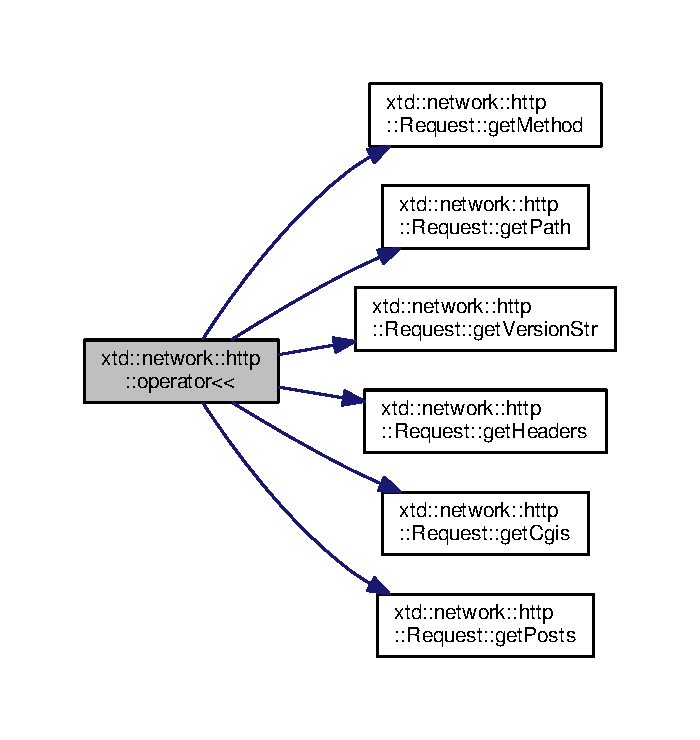
\includegraphics[width=336pt]{namespacextd_1_1network_1_1http_a9cd58530344372f236be8478d9c41ac3_cgraph}
\end{center}
\end{figure}



\hypertarget{namespacextd_1_1network_1_1http_1_1cpptempl}{}\section{xtd\+:\+:network\+:\+:http\+:\+:cpptempl Namespace Reference}
\label{namespacextd_1_1network_1_1http_1_1cpptempl}\index{xtd\+::network\+::http\+::cpptempl@{xtd\+::network\+::http\+::cpptempl}}
\subsection*{Classes}
\begin{DoxyCompactItemize}
\item 
class \hyperlink{classxtd_1_1network_1_1http_1_1cpptempl_1_1Data}{Data}
\item 
class \hyperlink{classxtd_1_1network_1_1http_1_1cpptempl_1_1DataList}{Data\+List}
\item 
class \hyperlink{classxtd_1_1network_1_1http_1_1cpptempl_1_1DataMap}{Data\+Map}
\item 
class \hyperlink{classxtd_1_1network_1_1http_1_1cpptempl_1_1DataValue}{Data\+Value}
\item 
class \hyperlink{classxtd_1_1network_1_1http_1_1cpptempl_1_1TemplateException}{Template\+Exception}
\item 
class \hyperlink{classxtd_1_1network_1_1http_1_1cpptempl_1_1Token}{Token}
\item 
class \hyperlink{classxtd_1_1network_1_1http_1_1cpptempl_1_1TokenEnd}{Token\+End}
\item 
class \hyperlink{classxtd_1_1network_1_1http_1_1cpptempl_1_1TokenFor}{Token\+For}
\item 
class \hyperlink{classxtd_1_1network_1_1http_1_1cpptempl_1_1TokenIf}{Token\+If}
\item 
class \hyperlink{classxtd_1_1network_1_1http_1_1cpptempl_1_1TokenText}{Token\+Text}
\item 
class \hyperlink{classxtd_1_1network_1_1http_1_1cpptempl_1_1TokenVar}{Token\+Var}
\end{DoxyCompactItemize}
\subsection*{Typedefs}
\begin{DoxyCompactItemize}
\item 
typedef boost\+::shared\+\_\+ptr$<$ \hyperlink{classxtd_1_1network_1_1http_1_1cpptempl_1_1Data}{Data} $>$ \hyperlink{namespacextd_1_1network_1_1http_1_1cpptempl_ad2f49991f1902699a98cf62bf0ae7ce6}{data\+\_\+ptr}
\item 
typedef vector$<$ \hyperlink{namespacextd_1_1network_1_1http_1_1cpptempl_ad2f49991f1902699a98cf62bf0ae7ce6}{data\+\_\+ptr} $>$ \hyperlink{namespacextd_1_1network_1_1http_1_1cpptempl_aff1b51bcf8064f69c85dd4833c1853b4}{data\+\_\+list}
\item 
typedef map$<$ string, \hyperlink{namespacextd_1_1network_1_1http_1_1cpptempl_ad2f49991f1902699a98cf62bf0ae7ce6}{data\+\_\+ptr} $>$ \hyperlink{namespacextd_1_1network_1_1http_1_1cpptempl_a638d1d81c8fb63c0bbafd508d6a2a007}{data\+\_\+map}
\item 
typedef boost\+::shared\+\_\+ptr$<$ \hyperlink{classxtd_1_1network_1_1http_1_1cpptempl_1_1Token}{Token} $>$ \hyperlink{namespacextd_1_1network_1_1http_1_1cpptempl_a09d1bd238d03342e60f0c20c679c0c88}{token\+\_\+ptr}
\item 
typedef vector$<$ \hyperlink{namespacextd_1_1network_1_1http_1_1cpptempl_a09d1bd238d03342e60f0c20c679c0c88}{token\+\_\+ptr} $>$ \hyperlink{namespacextd_1_1network_1_1http_1_1cpptempl_a38606cfbbfe81ed46ea9b0cf064de956}{token\+\_\+vector}
\end{DoxyCompactItemize}
\subsection*{Enumerations}
\begin{DoxyCompactItemize}
\item 
enum \hyperlink{namespacextd_1_1network_1_1http_1_1cpptempl_a39833083d228a5b5ef9f6bb7896479ee}{Token\+Type} \{ \\*
\hyperlink{namespacextd_1_1network_1_1http_1_1cpptempl_a39833083d228a5b5ef9f6bb7896479eeac2aec7f1ab8338419889ff04b8eb0f44}{T\+O\+K\+E\+N\+\_\+\+T\+Y\+P\+E\+\_\+\+N\+O\+NE}, 
\hyperlink{namespacextd_1_1network_1_1http_1_1cpptempl_a39833083d228a5b5ef9f6bb7896479eeaa3056860c42c00806c737551b598885c}{T\+O\+K\+E\+N\+\_\+\+T\+Y\+P\+E\+\_\+\+T\+E\+XT}, 
\hyperlink{namespacextd_1_1network_1_1http_1_1cpptempl_a39833083d228a5b5ef9f6bb7896479eea0e5df4476507663b07b952aefc096a86}{T\+O\+K\+E\+N\+\_\+\+T\+Y\+P\+E\+\_\+\+V\+AR}, 
\hyperlink{namespacextd_1_1network_1_1http_1_1cpptempl_a39833083d228a5b5ef9f6bb7896479eea63ca41e19f481129f654b675913cc557}{T\+O\+K\+E\+N\+\_\+\+T\+Y\+P\+E\+\_\+\+IF}, 
\\*
\hyperlink{namespacextd_1_1network_1_1http_1_1cpptempl_a39833083d228a5b5ef9f6bb7896479eea77914f6881c1bc9ec1910ca843bb6965}{T\+O\+K\+E\+N\+\_\+\+T\+Y\+P\+E\+\_\+\+F\+OR}, 
\hyperlink{namespacextd_1_1network_1_1http_1_1cpptempl_a39833083d228a5b5ef9f6bb7896479eea20879254cae890cea9ab4fbdb6223165}{T\+O\+K\+E\+N\+\_\+\+T\+Y\+P\+E\+\_\+\+E\+N\+D\+IF}, 
\hyperlink{namespacextd_1_1network_1_1http_1_1cpptempl_a39833083d228a5b5ef9f6bb7896479eea7a23df3b1f7078c58e56a3c51c24948c}{T\+O\+K\+E\+N\+\_\+\+T\+Y\+P\+E\+\_\+\+E\+N\+D\+F\+OR}
 \}
\end{DoxyCompactItemize}
\subsection*{Functions}
\begin{DoxyCompactItemize}
\item 
\hyperlink{namespacextd_1_1network_1_1http_1_1cpptempl_ad2f49991f1902699a98cf62bf0ae7ce6}{data\+\_\+ptr} \hyperlink{namespacextd_1_1network_1_1http_1_1cpptempl_af79d10d06cd5bc9ce629bb2d21fbcfd6}{parse\+\_\+val} (string key, \hyperlink{namespacextd_1_1network_1_1http_1_1cpptempl_a638d1d81c8fb63c0bbafd508d6a2a007}{data\+\_\+map} \&data)
\item 
void \hyperlink{namespacextd_1_1network_1_1http_1_1cpptempl_a27515db5dde2876849fa316963a67e63}{parse\+\_\+tree} (\hyperlink{namespacextd_1_1network_1_1http_1_1cpptempl_a38606cfbbfe81ed46ea9b0cf064de956}{token\+\_\+vector} \&tokens, \hyperlink{namespacextd_1_1network_1_1http_1_1cpptempl_a38606cfbbfe81ed46ea9b0cf064de956}{token\+\_\+vector} \&tree, \hyperlink{namespacextd_1_1network_1_1http_1_1cpptempl_a39833083d228a5b5ef9f6bb7896479ee}{Token\+Type} until)
\item 
\hyperlink{namespacextd_1_1network_1_1http_1_1cpptempl_a38606cfbbfe81ed46ea9b0cf064de956}{token\+\_\+vector} \& \hyperlink{namespacextd_1_1network_1_1http_1_1cpptempl_ab8c502f7e8347124c43f3dab3a583b34}{tokenize} (string text, \hyperlink{namespacextd_1_1network_1_1http_1_1cpptempl_a38606cfbbfe81ed46ea9b0cf064de956}{token\+\_\+vector} \&tokens)
\item 
string \hyperlink{namespacextd_1_1network_1_1http_1_1cpptempl_a10e259ee95bf5effff9095cdd140a058}{parse} (string templ\+\_\+text, \hyperlink{namespacextd_1_1network_1_1http_1_1cpptempl_a638d1d81c8fb63c0bbafd508d6a2a007}{data\+\_\+map} \&data)
\item 
\hyperlink{namespacextd_1_1network_1_1http_1_1cpptempl_ad2f49991f1902699a98cf62bf0ae7ce6}{data\+\_\+ptr} \hyperlink{namespacextd_1_1network_1_1http_1_1cpptempl_a32fe5ec0914372b09492647a168dbbcb}{make\+\_\+data} (string p\+\_\+val)
\item 
\hyperlink{namespacextd_1_1network_1_1http_1_1cpptempl_ad2f49991f1902699a98cf62bf0ae7ce6}{data\+\_\+ptr} \hyperlink{namespacextd_1_1network_1_1http_1_1cpptempl_aae0780ff5e5b2afd5996fb6d27ff8ca0}{make\+\_\+data} (\hyperlink{namespacextd_1_1network_1_1http_1_1cpptempl_aff1b51bcf8064f69c85dd4833c1853b4}{data\+\_\+list} \&p\+\_\+val)
\item 
\hyperlink{namespacextd_1_1network_1_1http_1_1cpptempl_ad2f49991f1902699a98cf62bf0ae7ce6}{data\+\_\+ptr} \hyperlink{namespacextd_1_1network_1_1http_1_1cpptempl_a4574c7173346efa3cfa420e5c657b58d}{make\+\_\+data} (\hyperlink{namespacextd_1_1network_1_1http_1_1cpptempl_a638d1d81c8fb63c0bbafd508d6a2a007}{data\+\_\+map} \&p\+\_\+val)
\item 
{\footnotesize template$<$typename T $>$ }\\\hyperlink{namespacextd_1_1network_1_1http_1_1cpptempl_ad2f49991f1902699a98cf62bf0ae7ce6}{data\+\_\+ptr} \hyperlink{namespacextd_1_1network_1_1http_1_1cpptempl_a290ac1d88dd4e0bcc65f955fb26e47c8}{make\+\_\+data} (T \&p\+\_\+val)
\item 
{\footnotesize template$<$typename T $>$ }\\\hyperlink{namespacextd_1_1network_1_1http_1_1cpptempl_ad2f49991f1902699a98cf62bf0ae7ce6}{data\+\_\+ptr} \hyperlink{namespacextd_1_1network_1_1http_1_1cpptempl_af97e4f705fc7cb54a179fe88293b2bd7}{make\+\_\+data} (vector$<$ T $>$ \&p\+\_\+val)
\item 
{\footnotesize template$<$typename T $>$ }\\\hyperlink{namespacextd_1_1network_1_1http_1_1cpptempl_ad2f49991f1902699a98cf62bf0ae7ce6}{data\+\_\+ptr} \hyperlink{namespacextd_1_1network_1_1http_1_1cpptempl_a9cfccbb6229825a04791ed3001f6500e}{make\+\_\+data} (map$<$ string, T $>$ \&p\+\_\+val)
\end{DoxyCompactItemize}


\subsection{Typedef Documentation}
\index{xtd\+::network\+::http\+::cpptempl@{xtd\+::network\+::http\+::cpptempl}!data\+\_\+list@{data\+\_\+list}}
\index{data\+\_\+list@{data\+\_\+list}!xtd\+::network\+::http\+::cpptempl@{xtd\+::network\+::http\+::cpptempl}}
\subsubsection[{\texorpdfstring{data\+\_\+list}{data_list}}]{\setlength{\rightskip}{0pt plus 5cm}typedef vector$<${\bf data\+\_\+ptr}$>$ {\bf xtd\+::network\+::http\+::cpptempl\+::data\+\_\+list}}\hypertarget{namespacextd_1_1network_1_1http_1_1cpptempl_aff1b51bcf8064f69c85dd4833c1853b4}{}\label{namespacextd_1_1network_1_1http_1_1cpptempl_aff1b51bcf8064f69c85dd4833c1853b4}


Definition at line 57 of file cpptempl.\+hh.

\index{xtd\+::network\+::http\+::cpptempl@{xtd\+::network\+::http\+::cpptempl}!data\+\_\+map@{data\+\_\+map}}
\index{data\+\_\+map@{data\+\_\+map}!xtd\+::network\+::http\+::cpptempl@{xtd\+::network\+::http\+::cpptempl}}
\subsubsection[{\texorpdfstring{data\+\_\+map}{data_map}}]{\setlength{\rightskip}{0pt plus 5cm}typedef map$<$string, {\bf data\+\_\+ptr}$>$ {\bf xtd\+::network\+::http\+::cpptempl\+::data\+\_\+map}}\hypertarget{namespacextd_1_1network_1_1http_1_1cpptempl_a638d1d81c8fb63c0bbafd508d6a2a007}{}\label{namespacextd_1_1network_1_1http_1_1cpptempl_a638d1d81c8fb63c0bbafd508d6a2a007}


Definition at line 58 of file cpptempl.\+hh.

\index{xtd\+::network\+::http\+::cpptempl@{xtd\+::network\+::http\+::cpptempl}!data\+\_\+ptr@{data\+\_\+ptr}}
\index{data\+\_\+ptr@{data\+\_\+ptr}!xtd\+::network\+::http\+::cpptempl@{xtd\+::network\+::http\+::cpptempl}}
\subsubsection[{\texorpdfstring{data\+\_\+ptr}{data_ptr}}]{\setlength{\rightskip}{0pt plus 5cm}typedef boost\+::shared\+\_\+ptr$<${\bf Data}$>$ {\bf xtd\+::network\+::http\+::cpptempl\+::data\+\_\+ptr}}\hypertarget{namespacextd_1_1network_1_1http_1_1cpptempl_ad2f49991f1902699a98cf62bf0ae7ce6}{}\label{namespacextd_1_1network_1_1http_1_1cpptempl_ad2f49991f1902699a98cf62bf0ae7ce6}


Definition at line 55 of file cpptempl.\+hh.

\index{xtd\+::network\+::http\+::cpptempl@{xtd\+::network\+::http\+::cpptempl}!token\+\_\+ptr@{token\+\_\+ptr}}
\index{token\+\_\+ptr@{token\+\_\+ptr}!xtd\+::network\+::http\+::cpptempl@{xtd\+::network\+::http\+::cpptempl}}
\subsubsection[{\texorpdfstring{token\+\_\+ptr}{token_ptr}}]{\setlength{\rightskip}{0pt plus 5cm}typedef boost\+::shared\+\_\+ptr$<${\bf Token}$>$ {\bf xtd\+::network\+::http\+::cpptempl\+::token\+\_\+ptr}}\hypertarget{namespacextd_1_1network_1_1http_1_1cpptempl_a09d1bd238d03342e60f0c20c679c0c88}{}\label{namespacextd_1_1network_1_1http_1_1cpptempl_a09d1bd238d03342e60f0c20c679c0c88}


Definition at line 60 of file cpptempl.\+hh.

\index{xtd\+::network\+::http\+::cpptempl@{xtd\+::network\+::http\+::cpptempl}!token\+\_\+vector@{token\+\_\+vector}}
\index{token\+\_\+vector@{token\+\_\+vector}!xtd\+::network\+::http\+::cpptempl@{xtd\+::network\+::http\+::cpptempl}}
\subsubsection[{\texorpdfstring{token\+\_\+vector}{token_vector}}]{\setlength{\rightskip}{0pt plus 5cm}typedef vector$<${\bf token\+\_\+ptr}$>$ {\bf xtd\+::network\+::http\+::cpptempl\+::token\+\_\+vector}}\hypertarget{namespacextd_1_1network_1_1http_1_1cpptempl_a38606cfbbfe81ed46ea9b0cf064de956}{}\label{namespacextd_1_1network_1_1http_1_1cpptempl_a38606cfbbfe81ed46ea9b0cf064de956}


Definition at line 62 of file cpptempl.\+hh.



\subsection{Enumeration Type Documentation}
\index{xtd\+::network\+::http\+::cpptempl@{xtd\+::network\+::http\+::cpptempl}!Token\+Type@{Token\+Type}}
\index{Token\+Type@{Token\+Type}!xtd\+::network\+::http\+::cpptempl@{xtd\+::network\+::http\+::cpptempl}}
\subsubsection[{\texorpdfstring{Token\+Type}{TokenType}}]{\setlength{\rightskip}{0pt plus 5cm}enum {\bf xtd\+::network\+::http\+::cpptempl\+::\+Token\+Type}}\hypertarget{namespacextd_1_1network_1_1http_1_1cpptempl_a39833083d228a5b5ef9f6bb7896479ee}{}\label{namespacextd_1_1network_1_1http_1_1cpptempl_a39833083d228a5b5ef9f6bb7896479ee}
\begin{Desc}
\item[Enumerator]\par
\begin{description}
\index{T\+O\+K\+E\+N\+\_\+\+T\+Y\+P\+E\+\_\+\+N\+O\+NE@{T\+O\+K\+E\+N\+\_\+\+T\+Y\+P\+E\+\_\+\+N\+O\+NE}!xtd\+::network\+::http\+::cpptempl@{xtd\+::network\+::http\+::cpptempl}}\index{xtd\+::network\+::http\+::cpptempl@{xtd\+::network\+::http\+::cpptempl}!T\+O\+K\+E\+N\+\_\+\+T\+Y\+P\+E\+\_\+\+N\+O\+NE@{T\+O\+K\+E\+N\+\_\+\+T\+Y\+P\+E\+\_\+\+N\+O\+NE}}\item[{\em 
T\+O\+K\+E\+N\+\_\+\+T\+Y\+P\+E\+\_\+\+N\+O\+NE\hypertarget{namespacextd_1_1network_1_1http_1_1cpptempl_a39833083d228a5b5ef9f6bb7896479eeac2aec7f1ab8338419889ff04b8eb0f44}{}\label{namespacextd_1_1network_1_1http_1_1cpptempl_a39833083d228a5b5ef9f6bb7896479eeac2aec7f1ab8338419889ff04b8eb0f44}
}]\index{T\+O\+K\+E\+N\+\_\+\+T\+Y\+P\+E\+\_\+\+T\+E\+XT@{T\+O\+K\+E\+N\+\_\+\+T\+Y\+P\+E\+\_\+\+T\+E\+XT}!xtd\+::network\+::http\+::cpptempl@{xtd\+::network\+::http\+::cpptempl}}\index{xtd\+::network\+::http\+::cpptempl@{xtd\+::network\+::http\+::cpptempl}!T\+O\+K\+E\+N\+\_\+\+T\+Y\+P\+E\+\_\+\+T\+E\+XT@{T\+O\+K\+E\+N\+\_\+\+T\+Y\+P\+E\+\_\+\+T\+E\+XT}}\item[{\em 
T\+O\+K\+E\+N\+\_\+\+T\+Y\+P\+E\+\_\+\+T\+E\+XT\hypertarget{namespacextd_1_1network_1_1http_1_1cpptempl_a39833083d228a5b5ef9f6bb7896479eeaa3056860c42c00806c737551b598885c}{}\label{namespacextd_1_1network_1_1http_1_1cpptempl_a39833083d228a5b5ef9f6bb7896479eeaa3056860c42c00806c737551b598885c}
}]\index{T\+O\+K\+E\+N\+\_\+\+T\+Y\+P\+E\+\_\+\+V\+AR@{T\+O\+K\+E\+N\+\_\+\+T\+Y\+P\+E\+\_\+\+V\+AR}!xtd\+::network\+::http\+::cpptempl@{xtd\+::network\+::http\+::cpptempl}}\index{xtd\+::network\+::http\+::cpptempl@{xtd\+::network\+::http\+::cpptempl}!T\+O\+K\+E\+N\+\_\+\+T\+Y\+P\+E\+\_\+\+V\+AR@{T\+O\+K\+E\+N\+\_\+\+T\+Y\+P\+E\+\_\+\+V\+AR}}\item[{\em 
T\+O\+K\+E\+N\+\_\+\+T\+Y\+P\+E\+\_\+\+V\+AR\hypertarget{namespacextd_1_1network_1_1http_1_1cpptempl_a39833083d228a5b5ef9f6bb7896479eea0e5df4476507663b07b952aefc096a86}{}\label{namespacextd_1_1network_1_1http_1_1cpptempl_a39833083d228a5b5ef9f6bb7896479eea0e5df4476507663b07b952aefc096a86}
}]\index{T\+O\+K\+E\+N\+\_\+\+T\+Y\+P\+E\+\_\+\+IF@{T\+O\+K\+E\+N\+\_\+\+T\+Y\+P\+E\+\_\+\+IF}!xtd\+::network\+::http\+::cpptempl@{xtd\+::network\+::http\+::cpptempl}}\index{xtd\+::network\+::http\+::cpptempl@{xtd\+::network\+::http\+::cpptempl}!T\+O\+K\+E\+N\+\_\+\+T\+Y\+P\+E\+\_\+\+IF@{T\+O\+K\+E\+N\+\_\+\+T\+Y\+P\+E\+\_\+\+IF}}\item[{\em 
T\+O\+K\+E\+N\+\_\+\+T\+Y\+P\+E\+\_\+\+IF\hypertarget{namespacextd_1_1network_1_1http_1_1cpptempl_a39833083d228a5b5ef9f6bb7896479eea63ca41e19f481129f654b675913cc557}{}\label{namespacextd_1_1network_1_1http_1_1cpptempl_a39833083d228a5b5ef9f6bb7896479eea63ca41e19f481129f654b675913cc557}
}]\index{T\+O\+K\+E\+N\+\_\+\+T\+Y\+P\+E\+\_\+\+F\+OR@{T\+O\+K\+E\+N\+\_\+\+T\+Y\+P\+E\+\_\+\+F\+OR}!xtd\+::network\+::http\+::cpptempl@{xtd\+::network\+::http\+::cpptempl}}\index{xtd\+::network\+::http\+::cpptempl@{xtd\+::network\+::http\+::cpptempl}!T\+O\+K\+E\+N\+\_\+\+T\+Y\+P\+E\+\_\+\+F\+OR@{T\+O\+K\+E\+N\+\_\+\+T\+Y\+P\+E\+\_\+\+F\+OR}}\item[{\em 
T\+O\+K\+E\+N\+\_\+\+T\+Y\+P\+E\+\_\+\+F\+OR\hypertarget{namespacextd_1_1network_1_1http_1_1cpptempl_a39833083d228a5b5ef9f6bb7896479eea77914f6881c1bc9ec1910ca843bb6965}{}\label{namespacextd_1_1network_1_1http_1_1cpptempl_a39833083d228a5b5ef9f6bb7896479eea77914f6881c1bc9ec1910ca843bb6965}
}]\index{T\+O\+K\+E\+N\+\_\+\+T\+Y\+P\+E\+\_\+\+E\+N\+D\+IF@{T\+O\+K\+E\+N\+\_\+\+T\+Y\+P\+E\+\_\+\+E\+N\+D\+IF}!xtd\+::network\+::http\+::cpptempl@{xtd\+::network\+::http\+::cpptempl}}\index{xtd\+::network\+::http\+::cpptempl@{xtd\+::network\+::http\+::cpptempl}!T\+O\+K\+E\+N\+\_\+\+T\+Y\+P\+E\+\_\+\+E\+N\+D\+IF@{T\+O\+K\+E\+N\+\_\+\+T\+Y\+P\+E\+\_\+\+E\+N\+D\+IF}}\item[{\em 
T\+O\+K\+E\+N\+\_\+\+T\+Y\+P\+E\+\_\+\+E\+N\+D\+IF\hypertarget{namespacextd_1_1network_1_1http_1_1cpptempl_a39833083d228a5b5ef9f6bb7896479eea20879254cae890cea9ab4fbdb6223165}{}\label{namespacextd_1_1network_1_1http_1_1cpptempl_a39833083d228a5b5ef9f6bb7896479eea20879254cae890cea9ab4fbdb6223165}
}]\index{T\+O\+K\+E\+N\+\_\+\+T\+Y\+P\+E\+\_\+\+E\+N\+D\+F\+OR@{T\+O\+K\+E\+N\+\_\+\+T\+Y\+P\+E\+\_\+\+E\+N\+D\+F\+OR}!xtd\+::network\+::http\+::cpptempl@{xtd\+::network\+::http\+::cpptempl}}\index{xtd\+::network\+::http\+::cpptempl@{xtd\+::network\+::http\+::cpptempl}!T\+O\+K\+E\+N\+\_\+\+T\+Y\+P\+E\+\_\+\+E\+N\+D\+F\+OR@{T\+O\+K\+E\+N\+\_\+\+T\+Y\+P\+E\+\_\+\+E\+N\+D\+F\+OR}}\item[{\em 
T\+O\+K\+E\+N\+\_\+\+T\+Y\+P\+E\+\_\+\+E\+N\+D\+F\+OR\hypertarget{namespacextd_1_1network_1_1http_1_1cpptempl_a39833083d228a5b5ef9f6bb7896479eea7a23df3b1f7078c58e56a3c51c24948c}{}\label{namespacextd_1_1network_1_1http_1_1cpptempl_a39833083d228a5b5ef9f6bb7896479eea7a23df3b1f7078c58e56a3c51c24948c}
}]\end{description}
\end{Desc}


Definition at line 176 of file cpptempl.\+hh.


\begin{DoxyCode}
177   \{
178     \hyperlink{namespacextd_1_1network_1_1http_1_1cpptempl_a39833083d228a5b5ef9f6bb7896479eeac2aec7f1ab8338419889ff04b8eb0f44}{TOKEN\_TYPE\_NONE},
179     \hyperlink{namespacextd_1_1network_1_1http_1_1cpptempl_a39833083d228a5b5ef9f6bb7896479eeaa3056860c42c00806c737551b598885c}{TOKEN\_TYPE\_TEXT},
180     \hyperlink{namespacextd_1_1network_1_1http_1_1cpptempl_a39833083d228a5b5ef9f6bb7896479eea0e5df4476507663b07b952aefc096a86}{TOKEN\_TYPE\_VAR},
181     \hyperlink{namespacextd_1_1network_1_1http_1_1cpptempl_a39833083d228a5b5ef9f6bb7896479eea63ca41e19f481129f654b675913cc557}{TOKEN\_TYPE\_IF},
182     \hyperlink{namespacextd_1_1network_1_1http_1_1cpptempl_a39833083d228a5b5ef9f6bb7896479eea77914f6881c1bc9ec1910ca843bb6965}{TOKEN\_TYPE\_FOR},
183     \hyperlink{namespacextd_1_1network_1_1http_1_1cpptempl_a39833083d228a5b5ef9f6bb7896479eea20879254cae890cea9ab4fbdb6223165}{TOKEN\_TYPE\_ENDIF},
184     \hyperlink{namespacextd_1_1network_1_1http_1_1cpptempl_a39833083d228a5b5ef9f6bb7896479eea7a23df3b1f7078c58e56a3c51c24948c}{TOKEN\_TYPE\_ENDFOR},
185   \} \hyperlink{namespacextd_1_1network_1_1http_1_1cpptempl_a39833083d228a5b5ef9f6bb7896479ee}{TokenType};
\end{DoxyCode}


\subsection{Function Documentation}
\index{xtd\+::network\+::http\+::cpptempl@{xtd\+::network\+::http\+::cpptempl}!make\+\_\+data@{make\+\_\+data}}
\index{make\+\_\+data@{make\+\_\+data}!xtd\+::network\+::http\+::cpptempl@{xtd\+::network\+::http\+::cpptempl}}
\subsubsection[{\texorpdfstring{make\+\_\+data(string p\+\_\+val)}{make_data(string p_val)}}]{\setlength{\rightskip}{0pt plus 5cm}{\bf data\+\_\+ptr} xtd\+::network\+::http\+::cpptempl\+::make\+\_\+data (
\begin{DoxyParamCaption}
\item[{string}]{p\+\_\+val}
\end{DoxyParamCaption}
)\hspace{0.3cm}{\ttfamily [inline]}}\hypertarget{namespacextd_1_1network_1_1http_1_1cpptempl_a32fe5ec0914372b09492647a168dbbcb}{}\label{namespacextd_1_1network_1_1http_1_1cpptempl_a32fe5ec0914372b09492647a168dbbcb}


Definition at line 128 of file cpptempl.\+hh.


\begin{DoxyCode}
129 \{
130   \textcolor{keywordflow}{return} \hyperlink{namespacextd_1_1network_1_1http_1_1cpptempl_ad2f49991f1902699a98cf62bf0ae7ce6}{data\_ptr}(\textcolor{keyword}{new} DataValue(p\_val));
131 \}
\end{DoxyCode}


Here is the caller graph for this function\+:
\nopagebreak
\begin{figure}[H]
\begin{center}
\leavevmode
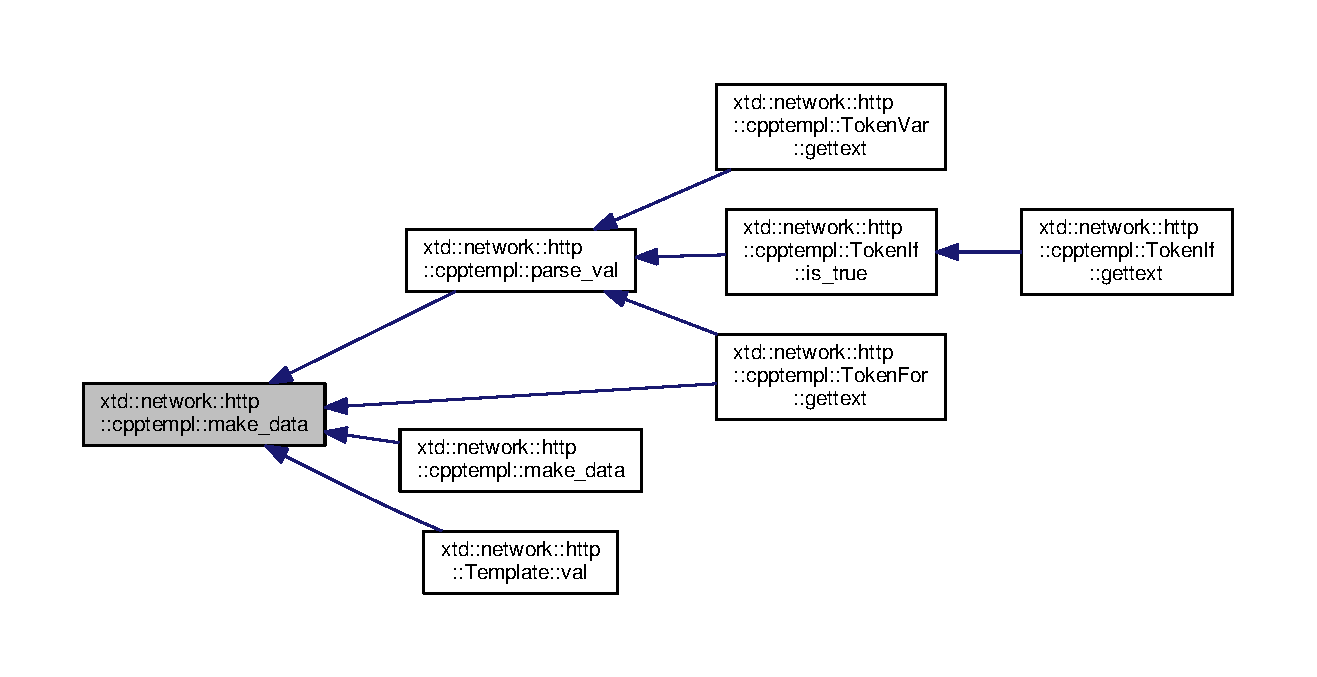
\includegraphics[width=350pt]{namespacextd_1_1network_1_1http_1_1cpptempl_a32fe5ec0914372b09492647a168dbbcb_icgraph}
\end{center}
\end{figure}


\index{xtd\+::network\+::http\+::cpptempl@{xtd\+::network\+::http\+::cpptempl}!make\+\_\+data@{make\+\_\+data}}
\index{make\+\_\+data@{make\+\_\+data}!xtd\+::network\+::http\+::cpptempl@{xtd\+::network\+::http\+::cpptempl}}
\subsubsection[{\texorpdfstring{make\+\_\+data(data\+\_\+list \&p\+\_\+val)}{make_data(data_list &p_val)}}]{\setlength{\rightskip}{0pt plus 5cm}{\bf data\+\_\+ptr} xtd\+::network\+::http\+::cpptempl\+::make\+\_\+data (
\begin{DoxyParamCaption}
\item[{{\bf data\+\_\+list} \&}]{p\+\_\+val}
\end{DoxyParamCaption}
)\hspace{0.3cm}{\ttfamily [inline]}}\hypertarget{namespacextd_1_1network_1_1http_1_1cpptempl_aae0780ff5e5b2afd5996fb6d27ff8ca0}{}\label{namespacextd_1_1network_1_1http_1_1cpptempl_aae0780ff5e5b2afd5996fb6d27ff8ca0}


Definition at line 133 of file cpptempl.\+hh.


\begin{DoxyCode}
134 \{
135   \textcolor{keywordflow}{return} \hyperlink{namespacextd_1_1network_1_1http_1_1cpptempl_ad2f49991f1902699a98cf62bf0ae7ce6}{data\_ptr}(\textcolor{keyword}{new} DataList(p\_val));
136 \}
\end{DoxyCode}
\index{xtd\+::network\+::http\+::cpptempl@{xtd\+::network\+::http\+::cpptempl}!make\+\_\+data@{make\+\_\+data}}
\index{make\+\_\+data@{make\+\_\+data}!xtd\+::network\+::http\+::cpptempl@{xtd\+::network\+::http\+::cpptempl}}
\subsubsection[{\texorpdfstring{make\+\_\+data(data\+\_\+map \&p\+\_\+val)}{make_data(data_map &p_val)}}]{\setlength{\rightskip}{0pt plus 5cm}{\bf data\+\_\+ptr} xtd\+::network\+::http\+::cpptempl\+::make\+\_\+data (
\begin{DoxyParamCaption}
\item[{{\bf data\+\_\+map} \&}]{p\+\_\+val}
\end{DoxyParamCaption}
)\hspace{0.3cm}{\ttfamily [inline]}}\hypertarget{namespacextd_1_1network_1_1http_1_1cpptempl_a4574c7173346efa3cfa420e5c657b58d}{}\label{namespacextd_1_1network_1_1http_1_1cpptempl_a4574c7173346efa3cfa420e5c657b58d}


Definition at line 138 of file cpptempl.\+hh.


\begin{DoxyCode}
139 \{
140   \textcolor{keywordflow}{return} \hyperlink{namespacextd_1_1network_1_1http_1_1cpptempl_ad2f49991f1902699a98cf62bf0ae7ce6}{data\_ptr}(\textcolor{keyword}{new} DataMap(p\_val));
141 \}
\end{DoxyCode}
\index{xtd\+::network\+::http\+::cpptempl@{xtd\+::network\+::http\+::cpptempl}!make\+\_\+data@{make\+\_\+data}}
\index{make\+\_\+data@{make\+\_\+data}!xtd\+::network\+::http\+::cpptempl@{xtd\+::network\+::http\+::cpptempl}}
\subsubsection[{\texorpdfstring{make\+\_\+data(\+T \&p\+\_\+val)}{make_data(T &p_val)}}]{\setlength{\rightskip}{0pt plus 5cm}template$<$typename T $>$ {\bf data\+\_\+ptr} xtd\+::network\+::http\+::cpptempl\+::make\+\_\+data (
\begin{DoxyParamCaption}
\item[{T \&}]{p\+\_\+val}
\end{DoxyParamCaption}
)\hspace{0.3cm}{\ttfamily [inline]}}\hypertarget{namespacextd_1_1network_1_1http_1_1cpptempl_a290ac1d88dd4e0bcc65f955fb26e47c8}{}\label{namespacextd_1_1network_1_1http_1_1cpptempl_a290ac1d88dd4e0bcc65f955fb26e47c8}


Definition at line 144 of file cpptempl.\+hh.


\begin{DoxyCode}
145 \{
146   \textcolor{keywordflow}{return} \hyperlink{namespacextd_1_1network_1_1http_1_1cpptempl_a9cfccbb6229825a04791ed3001f6500e}{make\_data}(boost::lexical\_cast<string>(p\_val));
147 \}
\end{DoxyCode}


Here is the call graph for this function\+:
\nopagebreak
\begin{figure}[H]
\begin{center}
\leavevmode
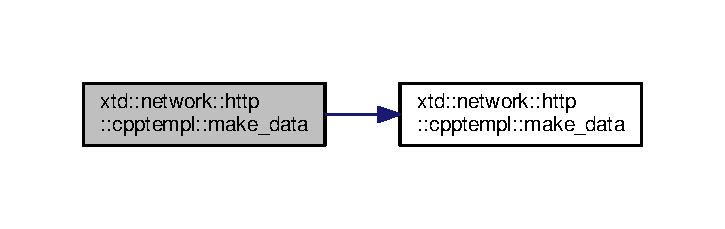
\includegraphics[width=348pt]{namespacextd_1_1network_1_1http_1_1cpptempl_a290ac1d88dd4e0bcc65f955fb26e47c8_cgraph}
\end{center}
\end{figure}


\index{xtd\+::network\+::http\+::cpptempl@{xtd\+::network\+::http\+::cpptempl}!make\+\_\+data@{make\+\_\+data}}
\index{make\+\_\+data@{make\+\_\+data}!xtd\+::network\+::http\+::cpptempl@{xtd\+::network\+::http\+::cpptempl}}
\subsubsection[{\texorpdfstring{make\+\_\+data(vector$<$ T $>$ \&p\+\_\+val)}{make_data(vector< T > &p_val)}}]{\setlength{\rightskip}{0pt plus 5cm}template$<$typename T $>$ {\bf data\+\_\+ptr} xtd\+::network\+::http\+::cpptempl\+::make\+\_\+data (
\begin{DoxyParamCaption}
\item[{vector$<$ T $>$ \&}]{p\+\_\+val}
\end{DoxyParamCaption}
)\hspace{0.3cm}{\ttfamily [inline]}}\hypertarget{namespacextd_1_1network_1_1http_1_1cpptempl_af97e4f705fc7cb54a179fe88293b2bd7}{}\label{namespacextd_1_1network_1_1http_1_1cpptempl_af97e4f705fc7cb54a179fe88293b2bd7}


Definition at line 150 of file cpptempl.\+hh.


\begin{DoxyCode}
151 \{
152   \hyperlink{namespacextd_1_1network_1_1http_1_1cpptempl_aff1b51bcf8064f69c85dd4833c1853b4}{data\_list}                         l\_list;
153   \textcolor{keyword}{typename} vector<T>::iterator c\_val;
154 
155   \textcolor{keywordflow}{for} (c\_val = p\_val.begin(); c\_val != p\_val.end(); c\_val++)
156     l\_list.push\_back(\hyperlink{namespacextd_1_1network_1_1http_1_1cpptempl_a9cfccbb6229825a04791ed3001f6500e}{make\_data}(*c\_val));
157   \textcolor{keywordflow}{return} \hyperlink{namespacextd_1_1network_1_1http_1_1cpptempl_a9cfccbb6229825a04791ed3001f6500e}{make\_data}(l\_list);
158 \}
\end{DoxyCode}


Here is the call graph for this function\+:
\nopagebreak
\begin{figure}[H]
\begin{center}
\leavevmode
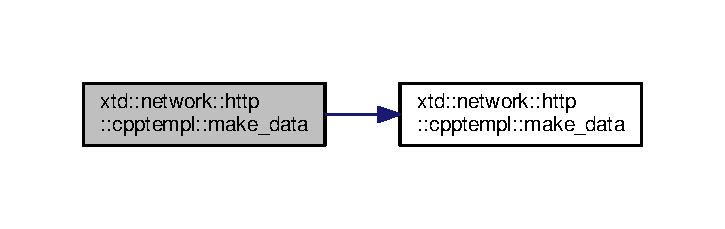
\includegraphics[width=348pt]{namespacextd_1_1network_1_1http_1_1cpptempl_af97e4f705fc7cb54a179fe88293b2bd7_cgraph}
\end{center}
\end{figure}


\index{xtd\+::network\+::http\+::cpptempl@{xtd\+::network\+::http\+::cpptempl}!make\+\_\+data@{make\+\_\+data}}
\index{make\+\_\+data@{make\+\_\+data}!xtd\+::network\+::http\+::cpptempl@{xtd\+::network\+::http\+::cpptempl}}
\subsubsection[{\texorpdfstring{make\+\_\+data(map$<$ string, T $>$ \&p\+\_\+val)}{make_data(map< string, T > &p_val)}}]{\setlength{\rightskip}{0pt plus 5cm}template$<$typename T $>$ {\bf data\+\_\+ptr} xtd\+::network\+::http\+::cpptempl\+::make\+\_\+data (
\begin{DoxyParamCaption}
\item[{map$<$ string, T $>$ \&}]{p\+\_\+val}
\end{DoxyParamCaption}
)\hspace{0.3cm}{\ttfamily [inline]}}\hypertarget{namespacextd_1_1network_1_1http_1_1cpptempl_a9cfccbb6229825a04791ed3001f6500e}{}\label{namespacextd_1_1network_1_1http_1_1cpptempl_a9cfccbb6229825a04791ed3001f6500e}


Definition at line 161 of file cpptempl.\+hh.


\begin{DoxyCode}
162 \{
163   \hyperlink{namespacextd_1_1network_1_1http_1_1cpptempl_a638d1d81c8fb63c0bbafd508d6a2a007}{data\_map}                                    l\_map;
164   \textcolor{keyword}{typename} map<string, T>::iterator c\_val;
165 
166   \textcolor{keywordflow}{for} (c\_val = p\_val.begin(); c\_val != p\_val.end(); c\_val++)
167     l\_map[c\_val->first] = \hyperlink{namespacextd_1_1network_1_1http_1_1cpptempl_a9cfccbb6229825a04791ed3001f6500e}{make\_data}(c\_val->second);
168 
169   \textcolor{keywordflow}{return} \hyperlink{namespacextd_1_1network_1_1http_1_1cpptempl_a9cfccbb6229825a04791ed3001f6500e}{make\_data}(l\_map);
170 \}
\end{DoxyCode}


Here is the call graph for this function\+:
\nopagebreak
\begin{figure}[H]
\begin{center}
\leavevmode
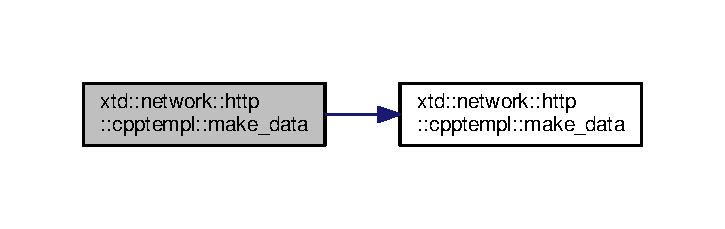
\includegraphics[width=350pt]{namespacextd_1_1network_1_1http_1_1cpptempl_a9cfccbb6229825a04791ed3001f6500e_cgraph}
\end{center}
\end{figure}


\index{xtd\+::network\+::http\+::cpptempl@{xtd\+::network\+::http\+::cpptempl}!parse@{parse}}
\index{parse@{parse}!xtd\+::network\+::http\+::cpptempl@{xtd\+::network\+::http\+::cpptempl}}
\subsubsection[{\texorpdfstring{parse(string templ\+\_\+text, data\+\_\+map \&data)}{parse(string templ_text, data_map &data)}}]{\setlength{\rightskip}{0pt plus 5cm}string xtd\+::network\+::http\+::cpptempl\+::parse (
\begin{DoxyParamCaption}
\item[{string}]{templ\+\_\+text, }
\item[{{\bf data\+\_\+map} \&}]{data}
\end{DoxyParamCaption}
)}\hypertarget{namespacextd_1_1network_1_1http_1_1cpptempl_a10e259ee95bf5effff9095cdd140a058}{}\label{namespacextd_1_1network_1_1http_1_1cpptempl_a10e259ee95bf5effff9095cdd140a058}


Definition at line 341 of file cpptempl.\+cc.


\begin{DoxyCode}
342 \{
343   \hyperlink{namespacextd_1_1network_1_1http_1_1cpptempl_a38606cfbbfe81ed46ea9b0cf064de956}{token\_vector} tokens;
344   \hyperlink{namespacextd_1_1network_1_1http_1_1cpptempl_ab8c502f7e8347124c43f3dab3a583b34}{tokenize}(templ\_text, tokens);
345   \hyperlink{namespacextd_1_1network_1_1http_1_1cpptempl_a38606cfbbfe81ed46ea9b0cf064de956}{token\_vector} tree;
346   \hyperlink{namespacextd_1_1network_1_1http_1_1cpptempl_a27515db5dde2876849fa316963a67e63}{parse\_tree}(tokens, tree);
347   vector<string> nodes;
348   \textcolor{keywordflow}{for} (\textcolor{keywordtype}{size\_t} i = 0; i < tree.size(); ++i)
349   \{
350     nodes.push\_back(tree[i]->gettext(data));
351   \}
352 
353   \textcolor{keywordflow}{return} boost::join(nodes, \textcolor{stringliteral}{""});
354 \}
\end{DoxyCode}


Here is the call graph for this function\+:
\nopagebreak
\begin{figure}[H]
\begin{center}
\leavevmode
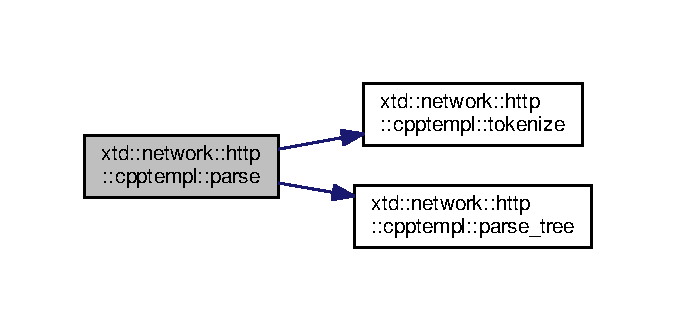
\includegraphics[width=323pt]{namespacextd_1_1network_1_1http_1_1cpptempl_a10e259ee95bf5effff9095cdd140a058_cgraph}
\end{center}
\end{figure}




Here is the caller graph for this function\+:
\nopagebreak
\begin{figure}[H]
\begin{center}
\leavevmode
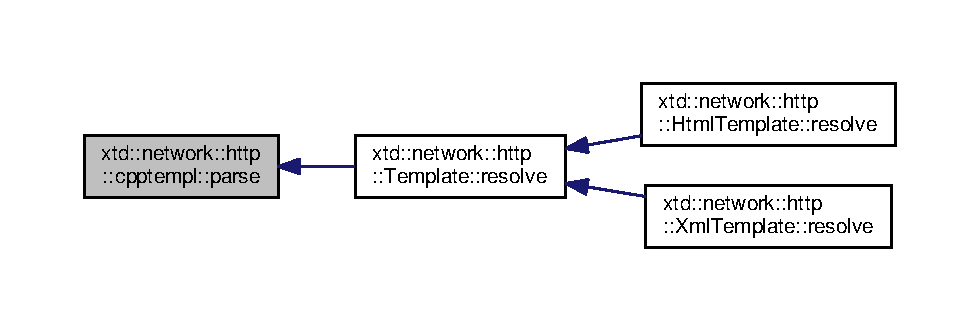
\includegraphics[width=350pt]{namespacextd_1_1network_1_1http_1_1cpptempl_a10e259ee95bf5effff9095cdd140a058_icgraph}
\end{center}
\end{figure}


\index{xtd\+::network\+::http\+::cpptempl@{xtd\+::network\+::http\+::cpptempl}!parse\+\_\+tree@{parse\+\_\+tree}}
\index{parse\+\_\+tree@{parse\+\_\+tree}!xtd\+::network\+::http\+::cpptempl@{xtd\+::network\+::http\+::cpptempl}}
\subsubsection[{\texorpdfstring{parse\+\_\+tree(token\+\_\+vector \&tokens, token\+\_\+vector \&tree, Token\+Type until)}{parse_tree(token_vector &tokens, token_vector &tree, TokenType until)}}]{\setlength{\rightskip}{0pt plus 5cm}void xtd\+::network\+::http\+::cpptempl\+::parse\+\_\+tree (
\begin{DoxyParamCaption}
\item[{{\bf token\+\_\+vector} \&}]{tokens, }
\item[{{\bf token\+\_\+vector} \&}]{tree, }
\item[{{\bf Token\+Type}}]{until}
\end{DoxyParamCaption}
)}\hypertarget{namespacextd_1_1network_1_1http_1_1cpptempl_a27515db5dde2876849fa316963a67e63}{}\label{namespacextd_1_1network_1_1http_1_1cpptempl_a27515db5dde2876849fa316963a67e63}


Definition at line 245 of file cpptempl.\+cc.


\begin{DoxyCode}
246 \{
247   \textcolor{keywordflow}{while}(! tokens.empty())
248   \{
249     \hyperlink{namespacextd_1_1network_1_1http_1_1cpptempl_a09d1bd238d03342e60f0c20c679c0c88}{token\_ptr} token = tokens[0];
250     tokens.erase(tokens.begin());
251     \textcolor{keywordflow}{if} (token->gettype() == \hyperlink{namespacextd_1_1network_1_1http_1_1cpptempl_a39833083d228a5b5ef9f6bb7896479eea77914f6881c1bc9ec1910ca843bb6965}{TOKEN\_TYPE\_FOR})
252     \{
253       \hyperlink{namespacextd_1_1network_1_1http_1_1cpptempl_a38606cfbbfe81ed46ea9b0cf064de956}{token\_vector} children;
254       \hyperlink{namespacextd_1_1network_1_1http_1_1cpptempl_a27515db5dde2876849fa316963a67e63}{parse\_tree}(tokens, children, \hyperlink{namespacextd_1_1network_1_1http_1_1cpptempl_a39833083d228a5b5ef9f6bb7896479eea7a23df3b1f7078c58e56a3c51c24948c}{TOKEN\_TYPE\_ENDFOR});
255       token->set\_children(children);
256     \}
257     \textcolor{keywordflow}{else} \textcolor{keywordflow}{if} (token->gettype() == \hyperlink{namespacextd_1_1network_1_1http_1_1cpptempl_a39833083d228a5b5ef9f6bb7896479eea63ca41e19f481129f654b675913cc557}{TOKEN\_TYPE\_IF})
258     \{
259       \hyperlink{namespacextd_1_1network_1_1http_1_1cpptempl_a38606cfbbfe81ed46ea9b0cf064de956}{token\_vector} children;
260       \hyperlink{namespacextd_1_1network_1_1http_1_1cpptempl_a27515db5dde2876849fa316963a67e63}{parse\_tree}(tokens, children, \hyperlink{namespacextd_1_1network_1_1http_1_1cpptempl_a39833083d228a5b5ef9f6bb7896479eea20879254cae890cea9ab4fbdb6223165}{TOKEN\_TYPE\_ENDIF});
261       token->set\_children(children);
262     \}
263     \textcolor{keywordflow}{else} \textcolor{keywordflow}{if} (token->gettype() == until)
264     \{
265       \textcolor{keywordflow}{return};
266     \}
267     tree.push\_back(token);
268   \}
269 \}
\end{DoxyCode}


Here is the caller graph for this function\+:
\nopagebreak
\begin{figure}[H]
\begin{center}
\leavevmode
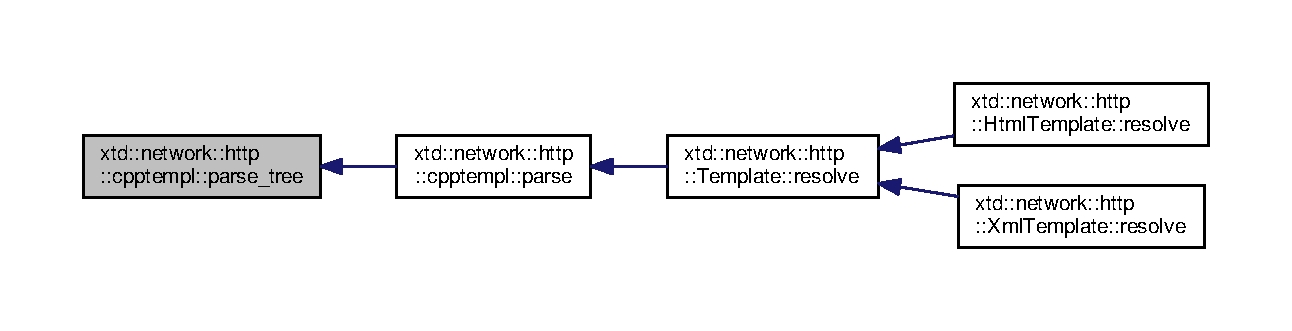
\includegraphics[width=350pt]{namespacextd_1_1network_1_1http_1_1cpptempl_a27515db5dde2876849fa316963a67e63_icgraph}
\end{center}
\end{figure}


\index{xtd\+::network\+::http\+::cpptempl@{xtd\+::network\+::http\+::cpptempl}!parse\+\_\+val@{parse\+\_\+val}}
\index{parse\+\_\+val@{parse\+\_\+val}!xtd\+::network\+::http\+::cpptempl@{xtd\+::network\+::http\+::cpptempl}}
\subsubsection[{\texorpdfstring{parse\+\_\+val(string key, data\+\_\+map \&data)}{parse_val(string key, data_map &data)}}]{\setlength{\rightskip}{0pt plus 5cm}{\bf data\+\_\+ptr} xtd\+::network\+::http\+::cpptempl\+::parse\+\_\+val (
\begin{DoxyParamCaption}
\item[{string}]{key, }
\item[{{\bf data\+\_\+map} \&}]{data}
\end{DoxyParamCaption}
)}\hypertarget{namespacextd_1_1network_1_1http_1_1cpptempl_af79d10d06cd5bc9ce629bb2d21fbcfd6}{}\label{namespacextd_1_1network_1_1http_1_1cpptempl_af79d10d06cd5bc9ce629bb2d21fbcfd6}


Definition at line 56 of file cpptempl.\+cc.


\begin{DoxyCode}
57 \{
58   data\_map::const\_iterator cc\_value;
59 
60   \textcolor{comment}{// quoted string}
61   \textcolor{keywordflow}{if} (key[0] == L\textcolor{charliteral}{'\(\backslash\)"'})
62   \{
63     \textcolor{keywordflow}{return} \hyperlink{namespacextd_1_1network_1_1http_1_1cpptempl_a32fe5ec0914372b09492647a168dbbcb}{make\_data}(boost::trim\_copy\_if(key, boost::is\_any\_of(\textcolor{stringliteral}{"\(\backslash\)""})));
64   \}
65   \textcolor{comment}{// check for dotted notation, i.e [foo.bar]}
66   \textcolor{keywordtype}{size\_t} index = key.find(\textcolor{stringliteral}{"."});
67   \textcolor{keywordflow}{if} (index == string::npos)
68   \{
69     \textcolor{keywordflow}{if} (data.end() == (cc\_value = data.find(key)))
70       \textcolor{keywordflow}{throw} TemplateException(boost::str(boost::format(\textcolor{stringliteral}{"unresolved key : %s"}) % key));
71     \textcolor{keywordflow}{return} cc\_value->second;
72   \}
73 
74   \textcolor{keywordflow}{if} (data.end() == (cc\_value = data.find(key.substr(0, index))))
75     \textcolor{keywordflow}{throw} TemplateException(boost::str(boost::format(\textcolor{stringliteral}{"unresolved key : %s"}) % key.substr(0, index)));
76 
77   \hyperlink{namespacextd_1_1network_1_1http_1_1cpptempl_ad2f49991f1902699a98cf62bf0ae7ce6}{data\_ptr} item = cc\_value->second;
78   \textcolor{keywordflow}{return} \hyperlink{namespacextd_1_1network_1_1http_1_1cpptempl_af79d10d06cd5bc9ce629bb2d21fbcfd6}{parse\_val}(key.substr(index+1), item->getmap());
79 \}
\end{DoxyCode}


Here is the call graph for this function\+:
\nopagebreak
\begin{figure}[H]
\begin{center}
\leavevmode
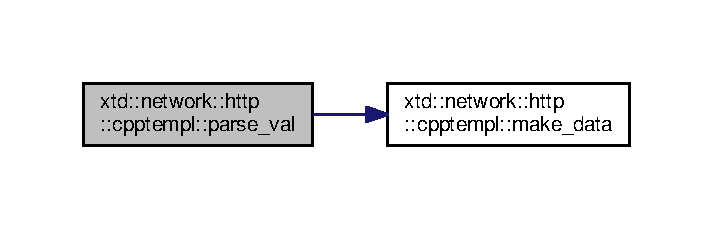
\includegraphics[width=342pt]{namespacextd_1_1network_1_1http_1_1cpptempl_af79d10d06cd5bc9ce629bb2d21fbcfd6_cgraph}
\end{center}
\end{figure}




Here is the caller graph for this function\+:
\nopagebreak
\begin{figure}[H]
\begin{center}
\leavevmode
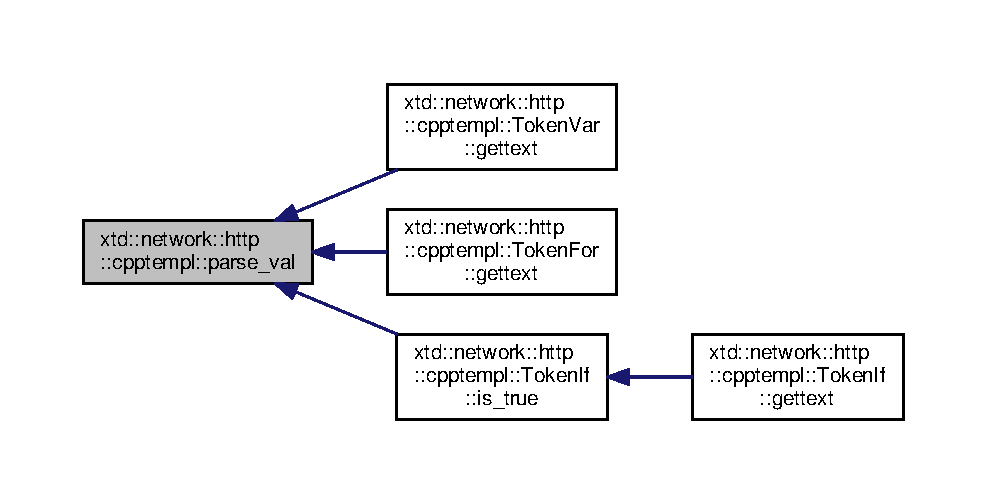
\includegraphics[width=342pt]{namespacextd_1_1network_1_1http_1_1cpptempl_af79d10d06cd5bc9ce629bb2d21fbcfd6_icgraph}
\end{center}
\end{figure}


\index{xtd\+::network\+::http\+::cpptempl@{xtd\+::network\+::http\+::cpptempl}!tokenize@{tokenize}}
\index{tokenize@{tokenize}!xtd\+::network\+::http\+::cpptempl@{xtd\+::network\+::http\+::cpptempl}}
\subsubsection[{\texorpdfstring{tokenize(string text, token\+\_\+vector \&tokens)}{tokenize(string text, token_vector &tokens)}}]{\setlength{\rightskip}{0pt plus 5cm}{\bf token\+\_\+vector} \& xtd\+::network\+::http\+::cpptempl\+::tokenize (
\begin{DoxyParamCaption}
\item[{string}]{text, }
\item[{{\bf token\+\_\+vector} \&}]{tokens}
\end{DoxyParamCaption}
)}\hypertarget{namespacextd_1_1network_1_1http_1_1cpptempl_ab8c502f7e8347124c43f3dab3a583b34}{}\label{namespacextd_1_1network_1_1http_1_1cpptempl_ab8c502f7e8347124c43f3dab3a583b34}


Definition at line 273 of file cpptempl.\+cc.


\begin{DoxyCode}
274 \{
275   \textcolor{keywordflow}{while}(\textcolor{keyword}{true})
276   \{
277     \textcolor{keywordtype}{size\_t} pos = text.find(\textcolor{stringliteral}{"\{"});
278     \textcolor{keywordflow}{if} (pos == string::npos)
279     \{
280       \textcolor{keywordflow}{if} (! text.empty())
281       \{
282         tokens.push\_back(\hyperlink{namespacextd_1_1network_1_1http_1_1cpptempl_a09d1bd238d03342e60f0c20c679c0c88}{token\_ptr}(\textcolor{keyword}{new} TokenText(text)));
283       \}
284       \textcolor{keywordflow}{return} tokens;
285     \}
286     \textcolor{keywordtype}{string} pre\_text = text.substr(0, pos);
287     \textcolor{keywordflow}{if} (! pre\_text.empty())
288     \{
289       tokens.push\_back(\hyperlink{namespacextd_1_1network_1_1http_1_1cpptempl_a09d1bd238d03342e60f0c20c679c0c88}{token\_ptr}(\textcolor{keyword}{new} TokenText(pre\_text)));
290     \}
291     text = text.substr(pos+1);
292     \textcolor{keywordflow}{if} (text.empty())
293     \{
294       tokens.push\_back(\hyperlink{namespacextd_1_1network_1_1http_1_1cpptempl_a09d1bd238d03342e60f0c20c679c0c88}{token\_ptr}(\textcolor{keyword}{new} TokenText(\textcolor{stringliteral}{"\{"})));
295       \textcolor{keywordflow}{return} tokens;
296     \}
297 
298     \textcolor{comment}{// variable}
299     \textcolor{keywordflow}{if} (text[0] == L\textcolor{charliteral}{'$'})
300     \{
301       pos = text.find(\textcolor{stringliteral}{"\}"});
302       \textcolor{keywordflow}{if} (pos != string::npos)
303       \{
304         tokens.push\_back(\hyperlink{namespacextd_1_1network_1_1http_1_1cpptempl_a09d1bd238d03342e60f0c20c679c0c88}{token\_ptr} (\textcolor{keyword}{new} TokenVar(text.substr(1, pos-1))));
305         text = text.substr(pos+1);
306       \}
307     \}
308     \textcolor{comment}{// control statement}
309     \textcolor{keywordflow}{else} \textcolor{keywordflow}{if} (text[0] == L\textcolor{charliteral}{'%'})
310     \{
311       pos = text.find(\textcolor{stringliteral}{"\}"});
312       \textcolor{keywordflow}{if} (pos != string::npos)
313       \{
314         \textcolor{keywordtype}{string} expression = boost::trim\_copy(text.substr(1, pos-2));
315         text = text.substr(pos+1);
316         \textcolor{keywordflow}{if} (boost::starts\_with(expression, \textcolor{stringliteral}{"for"}))
317         \{
318           tokens.push\_back(\hyperlink{namespacextd_1_1network_1_1http_1_1cpptempl_a09d1bd238d03342e60f0c20c679c0c88}{token\_ptr} (\textcolor{keyword}{new} TokenFor(expression)));
319         \}
320         \textcolor{keywordflow}{else} \textcolor{keywordflow}{if} (boost::starts\_with(expression, \textcolor{stringliteral}{"if"}))
321         \{
322           tokens.push\_back(\hyperlink{namespacextd_1_1network_1_1http_1_1cpptempl_a09d1bd238d03342e60f0c20c679c0c88}{token\_ptr} (\textcolor{keyword}{new} TokenIf(expression)));
323         \}
324         \textcolor{keywordflow}{else}
325         \{
326           tokens.push\_back(\hyperlink{namespacextd_1_1network_1_1http_1_1cpptempl_a09d1bd238d03342e60f0c20c679c0c88}{token\_ptr} (\textcolor{keyword}{new} TokenEnd(boost::trim\_copy(expression))));
327         \}
328       \}
329     \}
330     \textcolor{keywordflow}{else}
331     \{
332       tokens.push\_back(\hyperlink{namespacextd_1_1network_1_1http_1_1cpptempl_a09d1bd238d03342e60f0c20c679c0c88}{token\_ptr}(\textcolor{keyword}{new} TokenText(\textcolor{stringliteral}{"\{"})));
333     \}
334   \}
335   \textcolor{keywordflow}{return} tokens;
336 \}
\end{DoxyCode}


Here is the caller graph for this function\+:
\nopagebreak
\begin{figure}[H]
\begin{center}
\leavevmode
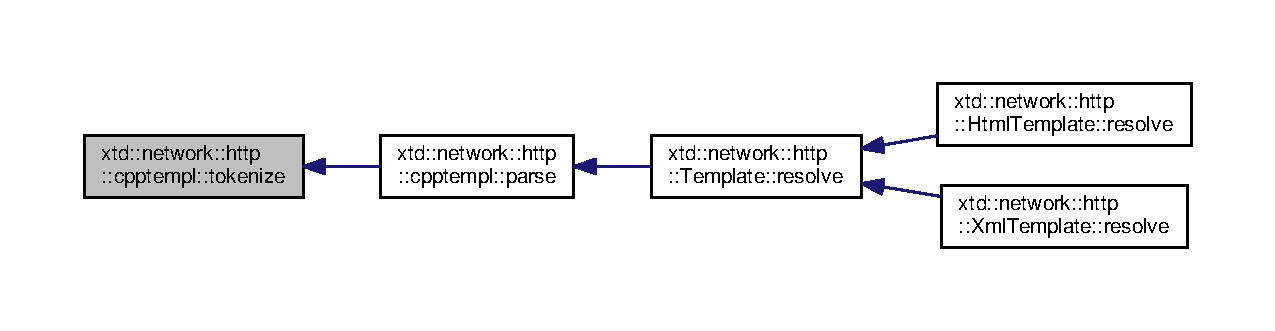
\includegraphics[width=350pt]{namespacextd_1_1network_1_1http_1_1cpptempl_ab8c502f7e8347124c43f3dab3a583b34_icgraph}
\end{center}
\end{figure}



\hypertarget{namespacextd_1_1network_1_1utils}{}\section{xtd\+:\+:network\+:\+:utils Namespace Reference}
\label{namespacextd_1_1network_1_1utils}\index{xtd\+::network\+::utils@{xtd\+::network\+::utils}}
\subsection*{Classes}
\begin{DoxyCompactItemize}
\item 
class \hyperlink{classxtd_1_1network_1_1utils_1_1CacheDns}{Cache\+Dns}
\begin{DoxyCompactList}\small\item\em Cache local de resolution de dns. \end{DoxyCompactList}\item 
struct \hyperlink{structxtd_1_1network_1_1utils_1_1CacheEntry}{Cache\+Entry}
\item 
class \hyperlink{classxtd_1_1network_1_1utils_1_1Config}{Config}
\item 
class \hyperlink{classxtd_1_1network_1_1utils_1_1deque__id}{deque\+\_\+id}
\item 
class \hyperlink{classxtd_1_1network_1_1utils_1_1Resolver}{Resolver}
\begin{DoxyCompactList}\small\item\em Resolution des noms de domaines. \end{DoxyCompactList}\item 
class \hyperlink{classxtd_1_1network_1_1utils_1_1Resolver_3_01af__inet_01_4}{Resolver$<$ af\+\_\+inet $>$}
\item 
class \hyperlink{classxtd_1_1network_1_1utils_1_1Resolver_3_01af__unix_01_4}{Resolver$<$ af\+\_\+unix $>$}
\item 
class \hyperlink{classxtd_1_1network_1_1utils_1_1scoped__method}{scoped\+\_\+method}
\item 
class \hyperlink{classxtd_1_1network_1_1utils_1_1vectorbuf}{vectorbuf}
\end{DoxyCompactItemize}
\subsection*{Typedefs}
\begin{DoxyCompactItemize}
\item 
typedef std\+::pair$<$ string, boost\+::shared\+\_\+ptr$<$ \hyperlink{structxtd_1_1network_1_1utils_1_1CacheEntry}{Cache\+Entry} $>$ $>$ \hyperlink{namespacextd_1_1network_1_1utils_a1118a93e3ee4c3aba74b90600794145b}{Entry\+Pair}
\begin{DoxyCompactList}\small\item\em typedef for U\+R\+L/\+Entry(IP address) pair \end{DoxyCompactList}\item 
typedef std\+::list$<$ boost\+::shared\+\_\+ptr$<$ \hyperlink{namespacextd_1_1network_1_1utils_a1118a93e3ee4c3aba74b90600794145b}{Entry\+Pair} $>$ $>$ \hyperlink{namespacextd_1_1network_1_1utils_a6eef494cdc6ca2b10bf4f36f6fa110ee}{Cache\+List}
\begin{DoxyCompactList}\small\item\em typedef for Cache list \end{DoxyCompactList}\item 
typedef boost\+::unordered\+\_\+map$<$ string, Cache\+List\+::iterator $>$ \hyperlink{namespacextd_1_1network_1_1utils_aa648e4975dce81f2fd0a9999f684781d}{Cache\+Map}
\begin{DoxyCompactList}\small\item\em typedef for U\+R\+L-\/indexed map (aka hash map) into the Cache\+List \end{DoxyCompactList}\item 
typedef boost\+::asio\+::deadline\+\_\+timer \hyperlink{namespacextd_1_1network_1_1utils_af551b4a44731a154a57b9447dac595cd}{dead\+Line\+Timer\+\_\+t}
\item 
typedef boost\+::shared\+\_\+ptr$<$ boost\+::asio\+::io\+\_\+service $>$ \hyperlink{namespacextd_1_1network_1_1utils_a67dfba91438896976d636d5aea36c848}{io\+Service\+Ptr\+\_\+t}
\item 
typedef boost\+::shared\+\_\+ptr$<$ boost\+::asio\+::io\+\_\+service\+::work $>$ \hyperlink{namespacextd_1_1network_1_1utils_a9e0bae7b0da2b42ca8930a927f3a7c4d}{work\+Ptr\+\_\+t}
\item 
typedef boost\+::shared\+\_\+ptr$<$ boost\+::asio\+::streambuf $>$ \hyperlink{namespacextd_1_1network_1_1utils_aaaf1b50be1864a40d85efd18979631e1}{streambuf\+Ptr\+\_\+t}
\item 
typedef map$<$ boost\+::thread\+::id, size\+\_\+t $>$ \hyperlink{namespacextd_1_1network_1_1utils_a778bf7884b2296561ffc1fc5a5f14e38}{t\+\_\+\+Id\+Number\+Map}
\item 
typedef std\+::pair$<$ boost\+::thread\+::id, size\+\_\+t $>$ \hyperlink{namespacextd_1_1network_1_1utils_aa6bd02256b6023347de116a773dd9500}{t\+\_\+\+Id\+Number\+Pair}
\item 
typedef boost\+::asio\+::local\+::stream\+\_\+protocol \hyperlink{namespacextd_1_1network_1_1utils_a60e83921a2d026f07b49fa094988acdf}{af\+\_\+unix}
\item 
typedef boost\+::asio\+::ip\+::tcp \hyperlink{namespacextd_1_1network_1_1utils_a6238bab7a616eda8c9424721444a18d1}{af\+\_\+inet}
\item 
typedef uint32\+\_\+t \hyperlink{namespacextd_1_1network_1_1utils_a0bdb4094852a77df867e219999175200}{request\+Id\+\_\+t}
\item 
typedef vector$<$ char $>$ \hyperlink{namespacextd_1_1network_1_1utils_a9fedf0d18549b8034e9ae347955e9a9a}{vector\+Bytes\+\_\+t}
\item 
typedef vector$<$ uint32\+\_\+t $>$ \hyperlink{namespacextd_1_1network_1_1utils_a2b135df55039cd8024b40ef3e1817681}{vector\+Uint32\+\_\+t}
\item 
typedef std\+::deque$<$ \hyperlink{namespacextd_1_1network_1_1utils_a0bdb4094852a77df867e219999175200}{request\+Id\+\_\+t} $>$ \hyperlink{namespacextd_1_1network_1_1utils_ac3ca189267ad1167fa141608f8b3a2de}{deque\+Id\+\_\+t}
\item 
typedef boost\+::shared\+\_\+ptr$<$ \hyperlink{namespacextd_1_1network_1_1utils_a9fedf0d18549b8034e9ae347955e9a9a}{vector\+Bytes\+\_\+t} $>$ \hyperlink{namespacextd_1_1network_1_1utils_a92b366b7e2a1ab09ac4f4a0401f8fb84}{shared\+Buf\+\_\+t}
\item 
typedef boost\+::shared\+\_\+ptr$<$ \hyperlink{namespacextd_1_1network_1_1utils_a2b135df55039cd8024b40ef3e1817681}{vector\+Uint32\+\_\+t} $>$ \hyperlink{namespacextd_1_1network_1_1utils_af5b287652a0fd8fca54642f8d3ca07fa}{shared\+Header\+\_\+t}
\item 
typedef boost\+::function$<$ void(const boost\+::system\+::error\+\_\+code)$>$ \hyperlink{namespacextd_1_1network_1_1utils_ac8a6f796cd645f83cde023d163665bb5}{handler\+\_\+t}
\end{DoxyCompactItemize}
\subsection*{Enumerations}
\begin{DoxyCompactItemize}
\item 
enum \hyperlink{namespacextd_1_1network_1_1utils_a0acc888a3cdabdadb91fe832ea196a4f}{option} \+: uint32\+\_\+t \{ \\*
\hyperlink{namespacextd_1_1network_1_1utils_a0acc888a3cdabdadb91fe832ea196a4faf0f888198330ff09558650aace4343e3}{option\+::nodelay} = 1, 
\hyperlink{namespacextd_1_1network_1_1utils_a0acc888a3cdabdadb91fe832ea196a4fa087d20314d2967622b76fbf7ce91ebf2}{option\+::reuseaddr} = 2, 
\hyperlink{namespacextd_1_1network_1_1utils_a0acc888a3cdabdadb91fe832ea196a4fa797919b5a9c95dfae9b06cf3086e40c1}{option\+::keepalive} = 4, 
\hyperlink{namespacextd_1_1network_1_1utils_a0acc888a3cdabdadb91fe832ea196a4fafa1711bb276806d1f1808dbb0e31018a}{option\+::linger} = 8, 
\\*
\hyperlink{namespacextd_1_1network_1_1utils_a0acc888a3cdabdadb91fe832ea196a4fa390626c545194d0f20a704589b190994}{option\+::compress} = 64
 \}
\item 
enum \hyperlink{namespacextd_1_1network_1_1utils_a3ac1216ad2037b366cc1f9051a978161}{codec} \+: uint32\+\_\+t \{ \hyperlink{namespacextd_1_1network_1_1utils_a3ac1216ad2037b366cc1f9051a978161a7a990d405d2c6fb93aa8fbb0ec1a3b23}{codec\+::zlib} = 1, 
\hyperlink{namespacextd_1_1network_1_1utils_a3ac1216ad2037b366cc1f9051a978161a749cadba7b2ed8d4a2aaa91a9cb1896c}{codec\+::gzip} = 2, 
\hyperlink{namespacextd_1_1network_1_1utils_a3ac1216ad2037b366cc1f9051a978161a03ce1ba314f367fdd09887fc8f60578b}{codec\+::bzip2} = 3
 \}
\end{DoxyCompactItemize}
\subsection*{Functions}
\begin{DoxyCompactItemize}
\item 
void \hyperlink{namespacextd_1_1network_1_1utils_a181758eb475ef5f4aebfec6c0ebec0c5}{do\+\_\+sem\+\_\+wait} (boost\+::interprocess\+::interprocess\+\_\+semaphore \&p\+\_\+sem)
\item 
std\+::time\+\_\+t \hyperlink{namespacextd_1_1network_1_1utils_aeee4bc5a0636807dd491f21938b7a1ca}{ptime\+\_\+to\+\_\+time\+\_\+t} (const boost\+::posix\+\_\+time\+::ptime \&t)
\end{DoxyCompactItemize}
\subsection*{Variables}
\begin{DoxyCompactItemize}
\item 
const uint32\+\_\+t \hyperlink{namespacextd_1_1network_1_1utils_a8939e806c4a6bc08b78a32941db7a130}{C\+A\+C\+H\+E\+\_\+\+C\+A\+P\+A\+C\+I\+T\+Y\+\_\+\+M\+AX} = 200
\item 
const uint32\+\_\+t \hyperlink{namespacextd_1_1network_1_1utils_adb4767541db3a79016a24142db705161}{C\+A\+C\+H\+E\+\_\+\+T\+T\+L\+\_\+\+M\+AX} = 1800
\end{DoxyCompactItemize}


\subsection{Typedef Documentation}
\index{xtd\+::network\+::utils@{xtd\+::network\+::utils}!af\+\_\+inet@{af\+\_\+inet}}
\index{af\+\_\+inet@{af\+\_\+inet}!xtd\+::network\+::utils@{xtd\+::network\+::utils}}
\subsubsection[{\texorpdfstring{af\+\_\+inet}{af_inet}}]{\setlength{\rightskip}{0pt plus 5cm}typedef boost\+::asio\+::ip\+::tcp {\bf xtd\+::network\+::utils\+::af\+\_\+inet}}\hypertarget{namespacextd_1_1network_1_1utils_a6238bab7a616eda8c9424721444a18d1}{}\label{namespacextd_1_1network_1_1utils_a6238bab7a616eda8c9424721444a18d1}


Definition at line 24 of file Comm\+Type\+Defs.\+hh.

\index{xtd\+::network\+::utils@{xtd\+::network\+::utils}!af\+\_\+unix@{af\+\_\+unix}}
\index{af\+\_\+unix@{af\+\_\+unix}!xtd\+::network\+::utils@{xtd\+::network\+::utils}}
\subsubsection[{\texorpdfstring{af\+\_\+unix}{af_unix}}]{\setlength{\rightskip}{0pt plus 5cm}typedef boost\+::asio\+::local\+::stream\+\_\+protocol {\bf xtd\+::network\+::utils\+::af\+\_\+unix}}\hypertarget{namespacextd_1_1network_1_1utils_a60e83921a2d026f07b49fa094988acdf}{}\label{namespacextd_1_1network_1_1utils_a60e83921a2d026f07b49fa094988acdf}


Definition at line 23 of file Comm\+Type\+Defs.\+hh.

\index{xtd\+::network\+::utils@{xtd\+::network\+::utils}!Cache\+List@{Cache\+List}}
\index{Cache\+List@{Cache\+List}!xtd\+::network\+::utils@{xtd\+::network\+::utils}}
\subsubsection[{\texorpdfstring{Cache\+List}{CacheList}}]{\setlength{\rightskip}{0pt plus 5cm}typedef std\+::list$<$ boost\+::shared\+\_\+ptr$<${\bf Entry\+Pair}$>$ $>$ {\bf xtd\+::network\+::utils\+::\+Cache\+List}}\hypertarget{namespacextd_1_1network_1_1utils_a6eef494cdc6ca2b10bf4f36f6fa110ee}{}\label{namespacextd_1_1network_1_1utils_a6eef494cdc6ca2b10bf4f36f6fa110ee}


typedef for Cache list 



Definition at line 47 of file Cache\+Dns.\+hh.

\index{xtd\+::network\+::utils@{xtd\+::network\+::utils}!Cache\+Map@{Cache\+Map}}
\index{Cache\+Map@{Cache\+Map}!xtd\+::network\+::utils@{xtd\+::network\+::utils}}
\subsubsection[{\texorpdfstring{Cache\+Map}{CacheMap}}]{\setlength{\rightskip}{0pt plus 5cm}typedef boost\+::unordered\+\_\+map$<$ string, Cache\+List\+::iterator $>$ {\bf xtd\+::network\+::utils\+::\+Cache\+Map}}\hypertarget{namespacextd_1_1network_1_1utils_aa648e4975dce81f2fd0a9999f684781d}{}\label{namespacextd_1_1network_1_1utils_aa648e4975dce81f2fd0a9999f684781d}


typedef for U\+R\+L-\/indexed map (aka hash map) into the Cache\+List 



Definition at line 49 of file Cache\+Dns.\+hh.

\index{xtd\+::network\+::utils@{xtd\+::network\+::utils}!dead\+Line\+Timer\+\_\+t@{dead\+Line\+Timer\+\_\+t}}
\index{dead\+Line\+Timer\+\_\+t@{dead\+Line\+Timer\+\_\+t}!xtd\+::network\+::utils@{xtd\+::network\+::utils}}
\subsubsection[{\texorpdfstring{dead\+Line\+Timer\+\_\+t}{deadLineTimer_t}}]{\setlength{\rightskip}{0pt plus 5cm}typedef boost\+::asio\+::deadline\+\_\+timer {\bf xtd\+::network\+::utils\+::dead\+Line\+Timer\+\_\+t}}\hypertarget{namespacextd_1_1network_1_1utils_af551b4a44731a154a57b9447dac595cd}{}\label{namespacextd_1_1network_1_1utils_af551b4a44731a154a57b9447dac595cd}


Definition at line 15 of file Comm\+Type\+Defs.\+hh.

\index{xtd\+::network\+::utils@{xtd\+::network\+::utils}!deque\+Id\+\_\+t@{deque\+Id\+\_\+t}}
\index{deque\+Id\+\_\+t@{deque\+Id\+\_\+t}!xtd\+::network\+::utils@{xtd\+::network\+::utils}}
\subsubsection[{\texorpdfstring{deque\+Id\+\_\+t}{dequeId_t}}]{\setlength{\rightskip}{0pt plus 5cm}typedef std\+::deque$<${\bf request\+Id\+\_\+t}$>$ {\bf xtd\+::network\+::utils\+::deque\+Id\+\_\+t}}\hypertarget{namespacextd_1_1network_1_1utils_ac3ca189267ad1167fa141608f8b3a2de}{}\label{namespacextd_1_1network_1_1utils_ac3ca189267ad1167fa141608f8b3a2de}


Definition at line 30 of file Comm\+Type\+Defs.\+hh.

\index{xtd\+::network\+::utils@{xtd\+::network\+::utils}!Entry\+Pair@{Entry\+Pair}}
\index{Entry\+Pair@{Entry\+Pair}!xtd\+::network\+::utils@{xtd\+::network\+::utils}}
\subsubsection[{\texorpdfstring{Entry\+Pair}{EntryPair}}]{\setlength{\rightskip}{0pt plus 5cm}typedef std\+::pair$<$ string, boost\+::shared\+\_\+ptr$<${\bf Cache\+Entry}$>$ $>$ {\bf xtd\+::network\+::utils\+::\+Entry\+Pair}}\hypertarget{namespacextd_1_1network_1_1utils_a1118a93e3ee4c3aba74b90600794145b}{}\label{namespacextd_1_1network_1_1utils_a1118a93e3ee4c3aba74b90600794145b}


typedef for U\+R\+L/\+Entry(IP address) pair 



Definition at line 45 of file Cache\+Dns.\+hh.

\index{xtd\+::network\+::utils@{xtd\+::network\+::utils}!handler\+\_\+t@{handler\+\_\+t}}
\index{handler\+\_\+t@{handler\+\_\+t}!xtd\+::network\+::utils@{xtd\+::network\+::utils}}
\subsubsection[{\texorpdfstring{handler\+\_\+t}{handler_t}}]{\setlength{\rightskip}{0pt plus 5cm}typedef boost\+::function$<$void(const boost\+::system\+::error\+\_\+code)$>$ {\bf xtd\+::network\+::utils\+::handler\+\_\+t}}\hypertarget{namespacextd_1_1network_1_1utils_ac8a6f796cd645f83cde023d163665bb5}{}\label{namespacextd_1_1network_1_1utils_ac8a6f796cd645f83cde023d163665bb5}


Definition at line 33 of file Comm\+Type\+Defs.\+hh.

\index{xtd\+::network\+::utils@{xtd\+::network\+::utils}!io\+Service\+Ptr\+\_\+t@{io\+Service\+Ptr\+\_\+t}}
\index{io\+Service\+Ptr\+\_\+t@{io\+Service\+Ptr\+\_\+t}!xtd\+::network\+::utils@{xtd\+::network\+::utils}}
\subsubsection[{\texorpdfstring{io\+Service\+Ptr\+\_\+t}{ioServicePtr_t}}]{\setlength{\rightskip}{0pt plus 5cm}typedef boost\+::shared\+\_\+ptr$<$boost\+::asio\+::io\+\_\+service$>$ {\bf xtd\+::network\+::utils\+::io\+Service\+Ptr\+\_\+t}}\hypertarget{namespacextd_1_1network_1_1utils_a67dfba91438896976d636d5aea36c848}{}\label{namespacextd_1_1network_1_1utils_a67dfba91438896976d636d5aea36c848}


Definition at line 16 of file Comm\+Type\+Defs.\+hh.

\index{xtd\+::network\+::utils@{xtd\+::network\+::utils}!request\+Id\+\_\+t@{request\+Id\+\_\+t}}
\index{request\+Id\+\_\+t@{request\+Id\+\_\+t}!xtd\+::network\+::utils@{xtd\+::network\+::utils}}
\subsubsection[{\texorpdfstring{request\+Id\+\_\+t}{requestId_t}}]{\setlength{\rightskip}{0pt plus 5cm}typedef uint32\+\_\+t {\bf xtd\+::network\+::utils\+::request\+Id\+\_\+t}}\hypertarget{namespacextd_1_1network_1_1utils_a0bdb4094852a77df867e219999175200}{}\label{namespacextd_1_1network_1_1utils_a0bdb4094852a77df867e219999175200}


Definition at line 25 of file Comm\+Type\+Defs.\+hh.

\index{xtd\+::network\+::utils@{xtd\+::network\+::utils}!shared\+Buf\+\_\+t@{shared\+Buf\+\_\+t}}
\index{shared\+Buf\+\_\+t@{shared\+Buf\+\_\+t}!xtd\+::network\+::utils@{xtd\+::network\+::utils}}
\subsubsection[{\texorpdfstring{shared\+Buf\+\_\+t}{sharedBuf_t}}]{\setlength{\rightskip}{0pt plus 5cm}typedef boost\+::shared\+\_\+ptr$<${\bf vector\+Bytes\+\_\+t}$>$ {\bf xtd\+::network\+::utils\+::shared\+Buf\+\_\+t}}\hypertarget{namespacextd_1_1network_1_1utils_a92b366b7e2a1ab09ac4f4a0401f8fb84}{}\label{namespacextd_1_1network_1_1utils_a92b366b7e2a1ab09ac4f4a0401f8fb84}


Definition at line 31 of file Comm\+Type\+Defs.\+hh.

\index{xtd\+::network\+::utils@{xtd\+::network\+::utils}!shared\+Header\+\_\+t@{shared\+Header\+\_\+t}}
\index{shared\+Header\+\_\+t@{shared\+Header\+\_\+t}!xtd\+::network\+::utils@{xtd\+::network\+::utils}}
\subsubsection[{\texorpdfstring{shared\+Header\+\_\+t}{sharedHeader_t}}]{\setlength{\rightskip}{0pt plus 5cm}typedef boost\+::shared\+\_\+ptr$<${\bf vector\+Uint32\+\_\+t}$>$ {\bf xtd\+::network\+::utils\+::shared\+Header\+\_\+t}}\hypertarget{namespacextd_1_1network_1_1utils_af5b287652a0fd8fca54642f8d3ca07fa}{}\label{namespacextd_1_1network_1_1utils_af5b287652a0fd8fca54642f8d3ca07fa}


Definition at line 32 of file Comm\+Type\+Defs.\+hh.

\index{xtd\+::network\+::utils@{xtd\+::network\+::utils}!streambuf\+Ptr\+\_\+t@{streambuf\+Ptr\+\_\+t}}
\index{streambuf\+Ptr\+\_\+t@{streambuf\+Ptr\+\_\+t}!xtd\+::network\+::utils@{xtd\+::network\+::utils}}
\subsubsection[{\texorpdfstring{streambuf\+Ptr\+\_\+t}{streambufPtr_t}}]{\setlength{\rightskip}{0pt plus 5cm}typedef boost\+::shared\+\_\+ptr$<$boost\+::asio\+::streambuf$>$ {\bf xtd\+::network\+::utils\+::streambuf\+Ptr\+\_\+t}}\hypertarget{namespacextd_1_1network_1_1utils_aaaf1b50be1864a40d85efd18979631e1}{}\label{namespacextd_1_1network_1_1utils_aaaf1b50be1864a40d85efd18979631e1}


Definition at line 18 of file Comm\+Type\+Defs.\+hh.

\index{xtd\+::network\+::utils@{xtd\+::network\+::utils}!t\+\_\+\+Id\+Number\+Map@{t\+\_\+\+Id\+Number\+Map}}
\index{t\+\_\+\+Id\+Number\+Map@{t\+\_\+\+Id\+Number\+Map}!xtd\+::network\+::utils@{xtd\+::network\+::utils}}
\subsubsection[{\texorpdfstring{t\+\_\+\+Id\+Number\+Map}{t_IdNumberMap}}]{\setlength{\rightskip}{0pt plus 5cm}typedef map$<$boost\+::thread\+::id, size\+\_\+t$>$ {\bf xtd\+::network\+::utils\+::t\+\_\+\+Id\+Number\+Map}}\hypertarget{namespacextd_1_1network_1_1utils_a778bf7884b2296561ffc1fc5a5f14e38}{}\label{namespacextd_1_1network_1_1utils_a778bf7884b2296561ffc1fc5a5f14e38}


Definition at line 19 of file Comm\+Type\+Defs.\+hh.

\index{xtd\+::network\+::utils@{xtd\+::network\+::utils}!t\+\_\+\+Id\+Number\+Pair@{t\+\_\+\+Id\+Number\+Pair}}
\index{t\+\_\+\+Id\+Number\+Pair@{t\+\_\+\+Id\+Number\+Pair}!xtd\+::network\+::utils@{xtd\+::network\+::utils}}
\subsubsection[{\texorpdfstring{t\+\_\+\+Id\+Number\+Pair}{t_IdNumberPair}}]{\setlength{\rightskip}{0pt plus 5cm}typedef std\+::pair$<$boost\+::thread\+::id, size\+\_\+t$>$ {\bf xtd\+::network\+::utils\+::t\+\_\+\+Id\+Number\+Pair}}\hypertarget{namespacextd_1_1network_1_1utils_aa6bd02256b6023347de116a773dd9500}{}\label{namespacextd_1_1network_1_1utils_aa6bd02256b6023347de116a773dd9500}


Definition at line 20 of file Comm\+Type\+Defs.\+hh.

\index{xtd\+::network\+::utils@{xtd\+::network\+::utils}!vector\+Bytes\+\_\+t@{vector\+Bytes\+\_\+t}}
\index{vector\+Bytes\+\_\+t@{vector\+Bytes\+\_\+t}!xtd\+::network\+::utils@{xtd\+::network\+::utils}}
\subsubsection[{\texorpdfstring{vector\+Bytes\+\_\+t}{vectorBytes_t}}]{\setlength{\rightskip}{0pt plus 5cm}typedef vector$<$char$>$ {\bf xtd\+::network\+::utils\+::vector\+Bytes\+\_\+t}}\hypertarget{namespacextd_1_1network_1_1utils_a9fedf0d18549b8034e9ae347955e9a9a}{}\label{namespacextd_1_1network_1_1utils_a9fedf0d18549b8034e9ae347955e9a9a}


Definition at line 28 of file Comm\+Type\+Defs.\+hh.

\index{xtd\+::network\+::utils@{xtd\+::network\+::utils}!vector\+Uint32\+\_\+t@{vector\+Uint32\+\_\+t}}
\index{vector\+Uint32\+\_\+t@{vector\+Uint32\+\_\+t}!xtd\+::network\+::utils@{xtd\+::network\+::utils}}
\subsubsection[{\texorpdfstring{vector\+Uint32\+\_\+t}{vectorUint32_t}}]{\setlength{\rightskip}{0pt plus 5cm}typedef vector$<$uint32\+\_\+t$>$ {\bf xtd\+::network\+::utils\+::vector\+Uint32\+\_\+t}}\hypertarget{namespacextd_1_1network_1_1utils_a2b135df55039cd8024b40ef3e1817681}{}\label{namespacextd_1_1network_1_1utils_a2b135df55039cd8024b40ef3e1817681}


Definition at line 29 of file Comm\+Type\+Defs.\+hh.

\index{xtd\+::network\+::utils@{xtd\+::network\+::utils}!work\+Ptr\+\_\+t@{work\+Ptr\+\_\+t}}
\index{work\+Ptr\+\_\+t@{work\+Ptr\+\_\+t}!xtd\+::network\+::utils@{xtd\+::network\+::utils}}
\subsubsection[{\texorpdfstring{work\+Ptr\+\_\+t}{workPtr_t}}]{\setlength{\rightskip}{0pt plus 5cm}typedef boost\+::shared\+\_\+ptr$<$boost\+::asio\+::io\+\_\+service\+::work$>$ {\bf xtd\+::network\+::utils\+::work\+Ptr\+\_\+t}}\hypertarget{namespacextd_1_1network_1_1utils_a9e0bae7b0da2b42ca8930a927f3a7c4d}{}\label{namespacextd_1_1network_1_1utils_a9e0bae7b0da2b42ca8930a927f3a7c4d}


Definition at line 17 of file Comm\+Type\+Defs.\+hh.



\subsection{Enumeration Type Documentation}
\index{xtd\+::network\+::utils@{xtd\+::network\+::utils}!codec@{codec}}
\index{codec@{codec}!xtd\+::network\+::utils@{xtd\+::network\+::utils}}
\subsubsection[{\texorpdfstring{codec}{codec}}]{\setlength{\rightskip}{0pt plus 5cm}enum {\bf xtd\+::network\+::utils\+::codec} \+: uint32\+\_\+t\hspace{0.3cm}{\ttfamily [strong]}}\hypertarget{namespacextd_1_1network_1_1utils_a3ac1216ad2037b366cc1f9051a978161}{}\label{namespacextd_1_1network_1_1utils_a3ac1216ad2037b366cc1f9051a978161}
\begin{Desc}
\item[Enumerator]\par
\begin{description}
\index{zlib@{zlib}!xtd\+::network\+::utils@{xtd\+::network\+::utils}}\index{xtd\+::network\+::utils@{xtd\+::network\+::utils}!zlib@{zlib}}\item[{\em 
zlib\hypertarget{namespacextd_1_1network_1_1utils_a3ac1216ad2037b366cc1f9051a978161a7a990d405d2c6fb93aa8fbb0ec1a3b23}{}\label{namespacextd_1_1network_1_1utils_a3ac1216ad2037b366cc1f9051a978161a7a990d405d2c6fb93aa8fbb0ec1a3b23}
}]\index{gzip@{gzip}!xtd\+::network\+::utils@{xtd\+::network\+::utils}}\index{xtd\+::network\+::utils@{xtd\+::network\+::utils}!gzip@{gzip}}\item[{\em 
gzip\hypertarget{namespacextd_1_1network_1_1utils_a3ac1216ad2037b366cc1f9051a978161a749cadba7b2ed8d4a2aaa91a9cb1896c}{}\label{namespacextd_1_1network_1_1utils_a3ac1216ad2037b366cc1f9051a978161a749cadba7b2ed8d4a2aaa91a9cb1896c}
}]\index{bzip2@{bzip2}!xtd\+::network\+::utils@{xtd\+::network\+::utils}}\index{xtd\+::network\+::utils@{xtd\+::network\+::utils}!bzip2@{bzip2}}\item[{\em 
bzip2\hypertarget{namespacextd_1_1network_1_1utils_a3ac1216ad2037b366cc1f9051a978161a03ce1ba314f367fdd09887fc8f60578b}{}\label{namespacextd_1_1network_1_1utils_a3ac1216ad2037b366cc1f9051a978161a03ce1ba314f367fdd09887fc8f60578b}
}]\end{description}
\end{Desc}


Definition at line 15 of file Config.\+hh.


\begin{DoxyCode}
15 : uint32\_t \{ \hyperlink{namespacextd_1_1network_1_1utils_a3ac1216ad2037b366cc1f9051a978161a7a990d405d2c6fb93aa8fbb0ec1a3b23}{zlib} = 1,    \hyperlink{namespacextd_1_1network_1_1utils_a3ac1216ad2037b366cc1f9051a978161a749cadba7b2ed8d4a2aaa91a9cb1896c}{gzip} = 2,      \hyperlink{namespacextd_1_1network_1_1utils_a3ac1216ad2037b366cc1f9051a978161a03ce1ba314f367fdd09887fc8f60578b}{bzip2} = 3 \};
\end{DoxyCode}
\index{xtd\+::network\+::utils@{xtd\+::network\+::utils}!option@{option}}
\index{option@{option}!xtd\+::network\+::utils@{xtd\+::network\+::utils}}
\subsubsection[{\texorpdfstring{option}{option}}]{\setlength{\rightskip}{0pt plus 5cm}enum {\bf xtd\+::network\+::utils\+::option} \+: uint32\+\_\+t\hspace{0.3cm}{\ttfamily [strong]}}\hypertarget{namespacextd_1_1network_1_1utils_a0acc888a3cdabdadb91fe832ea196a4f}{}\label{namespacextd_1_1network_1_1utils_a0acc888a3cdabdadb91fe832ea196a4f}
\begin{Desc}
\item[Enumerator]\par
\begin{description}
\index{nodelay@{nodelay}!xtd\+::network\+::utils@{xtd\+::network\+::utils}}\index{xtd\+::network\+::utils@{xtd\+::network\+::utils}!nodelay@{nodelay}}\item[{\em 
nodelay\hypertarget{namespacextd_1_1network_1_1utils_a0acc888a3cdabdadb91fe832ea196a4faf0f888198330ff09558650aace4343e3}{}\label{namespacextd_1_1network_1_1utils_a0acc888a3cdabdadb91fe832ea196a4faf0f888198330ff09558650aace4343e3}
}]\index{reuseaddr@{reuseaddr}!xtd\+::network\+::utils@{xtd\+::network\+::utils}}\index{xtd\+::network\+::utils@{xtd\+::network\+::utils}!reuseaddr@{reuseaddr}}\item[{\em 
reuseaddr\hypertarget{namespacextd_1_1network_1_1utils_a0acc888a3cdabdadb91fe832ea196a4fa087d20314d2967622b76fbf7ce91ebf2}{}\label{namespacextd_1_1network_1_1utils_a0acc888a3cdabdadb91fe832ea196a4fa087d20314d2967622b76fbf7ce91ebf2}
}]\index{keepalive@{keepalive}!xtd\+::network\+::utils@{xtd\+::network\+::utils}}\index{xtd\+::network\+::utils@{xtd\+::network\+::utils}!keepalive@{keepalive}}\item[{\em 
keepalive\hypertarget{namespacextd_1_1network_1_1utils_a0acc888a3cdabdadb91fe832ea196a4fa797919b5a9c95dfae9b06cf3086e40c1}{}\label{namespacextd_1_1network_1_1utils_a0acc888a3cdabdadb91fe832ea196a4fa797919b5a9c95dfae9b06cf3086e40c1}
}]\index{linger@{linger}!xtd\+::network\+::utils@{xtd\+::network\+::utils}}\index{xtd\+::network\+::utils@{xtd\+::network\+::utils}!linger@{linger}}\item[{\em 
linger\hypertarget{namespacextd_1_1network_1_1utils_a0acc888a3cdabdadb91fe832ea196a4fafa1711bb276806d1f1808dbb0e31018a}{}\label{namespacextd_1_1network_1_1utils_a0acc888a3cdabdadb91fe832ea196a4fafa1711bb276806d1f1808dbb0e31018a}
}]\index{compress@{compress}!xtd\+::network\+::utils@{xtd\+::network\+::utils}}\index{xtd\+::network\+::utils@{xtd\+::network\+::utils}!compress@{compress}}\item[{\em 
compress\hypertarget{namespacextd_1_1network_1_1utils_a0acc888a3cdabdadb91fe832ea196a4fa390626c545194d0f20a704589b190994}{}\label{namespacextd_1_1network_1_1utils_a0acc888a3cdabdadb91fe832ea196a4fa390626c545194d0f20a704589b190994}
}]\end{description}
\end{Desc}


Definition at line 14 of file Config.\+hh.


\begin{DoxyCode}
14 : uint32\_t \{ \hyperlink{namespacextd_1_1network_1_1utils_a0acc888a3cdabdadb91fe832ea196a4faf0f888198330ff09558650aace4343e3}{nodelay} = 1, \hyperlink{namespacextd_1_1network_1_1utils_a0acc888a3cdabdadb91fe832ea196a4fa087d20314d2967622b76fbf7ce91ebf2}{reuseaddr} = 2, \hyperlink{namespacextd_1_1network_1_1utils_a0acc888a3cdabdadb91fe832ea196a4fa797919b5a9c95dfae9b06cf3086e40c1}{keepalive} = 4, 
      \hyperlink{namespacextd_1_1network_1_1utils_a0acc888a3cdabdadb91fe832ea196a4fafa1711bb276806d1f1808dbb0e31018a}{linger} = 8, \hyperlink{namespacextd_1_1network_1_1utils_a0acc888a3cdabdadb91fe832ea196a4fa390626c545194d0f20a704589b190994}{compress} = 64 \};
\end{DoxyCode}


\subsection{Function Documentation}
\index{xtd\+::network\+::utils@{xtd\+::network\+::utils}!do\+\_\+sem\+\_\+wait@{do\+\_\+sem\+\_\+wait}}
\index{do\+\_\+sem\+\_\+wait@{do\+\_\+sem\+\_\+wait}!xtd\+::network\+::utils@{xtd\+::network\+::utils}}
\subsubsection[{\texorpdfstring{do\+\_\+sem\+\_\+wait(boost\+::interprocess\+::interprocess\+\_\+semaphore \&p\+\_\+sem)}{do_sem_wait(boost::interprocess::interprocess_semaphore &p_sem)}}]{\setlength{\rightskip}{0pt plus 5cm}void xtd\+::network\+::utils\+::do\+\_\+sem\+\_\+wait (
\begin{DoxyParamCaption}
\item[{boost\+::interprocess\+::interprocess\+\_\+semaphore \&}]{p\+\_\+sem}
\end{DoxyParamCaption}
)}\hypertarget{namespacextd_1_1network_1_1utils_a181758eb475ef5f4aebfec6c0ebec0c5}{}\label{namespacextd_1_1network_1_1utils_a181758eb475ef5f4aebfec6c0ebec0c5}


Definition at line 9 of file Utils.\+cc.


\begin{DoxyCode}
10 \{
11   \textcolor{keywordflow}{try}
12   \{
13     p\_sem.wait();
14   \}
15   \textcolor{keywordflow}{catch}(boost::interprocess::interprocess\_exception e)
16   \{
17     \textcolor{keywordflow}{if} (e.get\_native\_error() == EINTR)
18     \{
19       \hyperlink{namespacextd_1_1network_1_1utils_a181758eb475ef5f4aebfec6c0ebec0c5}{do\_sem\_wait}(p\_sem);
20     \}
21   \}
22 \};
\end{DoxyCode}
\index{xtd\+::network\+::utils@{xtd\+::network\+::utils}!ptime\+\_\+to\+\_\+time\+\_\+t@{ptime\+\_\+to\+\_\+time\+\_\+t}}
\index{ptime\+\_\+to\+\_\+time\+\_\+t@{ptime\+\_\+to\+\_\+time\+\_\+t}!xtd\+::network\+::utils@{xtd\+::network\+::utils}}
\subsubsection[{\texorpdfstring{ptime\+\_\+to\+\_\+time\+\_\+t(const boost\+::posix\+\_\+time\+::ptime \&t)}{ptime_to_time_t(const boost::posix_time::ptime &t)}}]{\setlength{\rightskip}{0pt plus 5cm}std\+::time\+\_\+t xtd\+::network\+::utils\+::ptime\+\_\+to\+\_\+time\+\_\+t (
\begin{DoxyParamCaption}
\item[{const boost\+::posix\+\_\+time\+::ptime \&}]{t}
\end{DoxyParamCaption}
)}\hypertarget{namespacextd_1_1network_1_1utils_aeee4bc5a0636807dd491f21938b7a1ca}{}\label{namespacextd_1_1network_1_1utils_aeee4bc5a0636807dd491f21938b7a1ca}


Definition at line 26 of file Utils.\+cc.


\begin{DoxyCode}
27 \{
28   \textcolor{keyword}{static} \textcolor{keyword}{const} boost::posix\_time::ptime epoch(boost::gregorian::date(1970,1,1) );
29   \textcolor{keyword}{const} boost::posix\_time::time\_duration::sec\_type ss((t - epoch).total\_seconds() );
30   \textcolor{keywordflow}{return} ss;
31 \}
\end{DoxyCode}


Here is the caller graph for this function\+:
\nopagebreak
\begin{figure}[H]
\begin{center}
\leavevmode
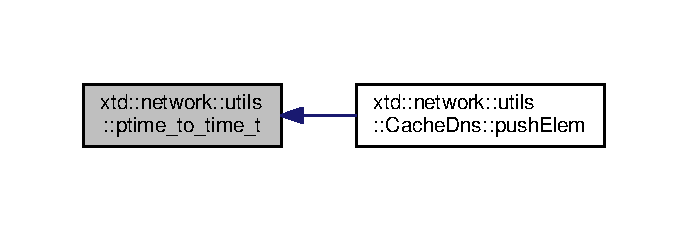
\includegraphics[width=330pt]{namespacextd_1_1network_1_1utils_aeee4bc5a0636807dd491f21938b7a1ca_icgraph}
\end{center}
\end{figure}




\subsection{Variable Documentation}
\index{xtd\+::network\+::utils@{xtd\+::network\+::utils}!C\+A\+C\+H\+E\+\_\+\+C\+A\+P\+A\+C\+I\+T\+Y\+\_\+\+M\+AX@{C\+A\+C\+H\+E\+\_\+\+C\+A\+P\+A\+C\+I\+T\+Y\+\_\+\+M\+AX}}
\index{C\+A\+C\+H\+E\+\_\+\+C\+A\+P\+A\+C\+I\+T\+Y\+\_\+\+M\+AX@{C\+A\+C\+H\+E\+\_\+\+C\+A\+P\+A\+C\+I\+T\+Y\+\_\+\+M\+AX}!xtd\+::network\+::utils@{xtd\+::network\+::utils}}
\subsubsection[{\texorpdfstring{C\+A\+C\+H\+E\+\_\+\+C\+A\+P\+A\+C\+I\+T\+Y\+\_\+\+M\+AX}{CACHE_CAPACITY_MAX}}]{\setlength{\rightskip}{0pt plus 5cm}const uint32\+\_\+t xtd\+::network\+::utils\+::\+C\+A\+C\+H\+E\+\_\+\+C\+A\+P\+A\+C\+I\+T\+Y\+\_\+\+M\+AX = 200}\hypertarget{namespacextd_1_1network_1_1utils_a8939e806c4a6bc08b78a32941db7a130}{}\label{namespacextd_1_1network_1_1utils_a8939e806c4a6bc08b78a32941db7a130}


Definition at line 29 of file Cache\+Dns.\+hh.

\index{xtd\+::network\+::utils@{xtd\+::network\+::utils}!C\+A\+C\+H\+E\+\_\+\+T\+T\+L\+\_\+\+M\+AX@{C\+A\+C\+H\+E\+\_\+\+T\+T\+L\+\_\+\+M\+AX}}
\index{C\+A\+C\+H\+E\+\_\+\+T\+T\+L\+\_\+\+M\+AX@{C\+A\+C\+H\+E\+\_\+\+T\+T\+L\+\_\+\+M\+AX}!xtd\+::network\+::utils@{xtd\+::network\+::utils}}
\subsubsection[{\texorpdfstring{C\+A\+C\+H\+E\+\_\+\+T\+T\+L\+\_\+\+M\+AX}{CACHE_TTL_MAX}}]{\setlength{\rightskip}{0pt plus 5cm}const uint32\+\_\+t xtd\+::network\+::utils\+::\+C\+A\+C\+H\+E\+\_\+\+T\+T\+L\+\_\+\+M\+AX = 1800}\hypertarget{namespacextd_1_1network_1_1utils_adb4767541db3a79016a24142db705161}{}\label{namespacextd_1_1network_1_1utils_adb4767541db3a79016a24142db705161}


Definition at line 30 of file Cache\+Dns.\+hh.


\chapter{Class Documentation}
\hypertarget{classxtd_1_1network_1_1utils_1_1CacheDns}{\section{xtd\-:\-:network\-:\-:utils\-:\-:Cache\-Dns Class Reference}
\label{classxtd_1_1network_1_1utils_1_1CacheDns}\index{xtd\-::network\-::utils\-::\-Cache\-Dns@{xtd\-::network\-::utils\-::\-Cache\-Dns}}
}


Cache local de resolution de dns.  




{\ttfamily \#include $<$Cache\-Dns.\-hh$>$}



Inheritance diagram for xtd\-:\-:network\-:\-:utils\-:\-:Cache\-Dns\-:
\nopagebreak
\begin{figure}[H]
\begin{center}
\leavevmode
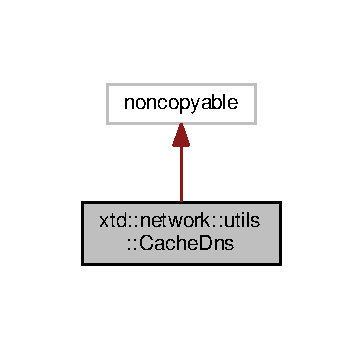
\includegraphics[width=174pt]{classxtd_1_1network_1_1utils_1_1CacheDns__inherit__graph}
\end{center}
\end{figure}


Collaboration diagram for xtd\-:\-:network\-:\-:utils\-:\-:Cache\-Dns\-:
\nopagebreak
\begin{figure}[H]
\begin{center}
\leavevmode
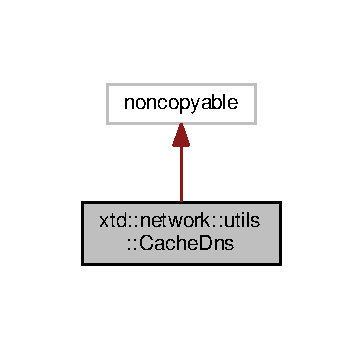
\includegraphics[width=174pt]{classxtd_1_1network_1_1utils_1_1CacheDns__coll__graph}
\end{center}
\end{figure}
\subsection*{Public Member Functions}
\begin{DoxyCompactItemize}
\item 
\hyperlink{classxtd_1_1network_1_1utils_1_1CacheDns_ac74635760f1d9fb738d940e3dc723476}{Cache\-Dns} (uint32\-\_\-t p\-\_\-capacity, uint32\-\_\-t p\-\_\-ttl)
\begin{DoxyCompactList}\small\item\em Cache D\-N\-S Constructor specifying capacity and entry timetolive. \end{DoxyCompactList}\item 
bool \hyperlink{classxtd_1_1network_1_1utils_1_1CacheDns_ab409d08cb0159d6250db8d1d05c6617b}{pop\-Elem} (const string \&p\-\_\-url, string \&p\-\_\-ip\-Addr)
\begin{DoxyCompactList}\small\item\em pop the element from the pool \end{DoxyCompactList}\item 
void \hyperlink{classxtd_1_1network_1_1utils_1_1CacheDns_a1ac8401e5827dbfbc39a909c2cf7afdf}{push\-Elem} (const string \&p\-\_\-url, const string \&p\-\_\-ip\-Addr)
\begin{DoxyCompactList}\small\item\em push the element in the pool \end{DoxyCompactList}\item 
size\-\_\-t \hyperlink{classxtd_1_1network_1_1utils_1_1CacheDns_a05377d5ccc35a6ba0f6e7124c891be37}{size} (void) const 
\begin{DoxyCompactList}\small\item\em Returns the number of elements present in the cache dns. \end{DoxyCompactList}\end{DoxyCompactItemize}


\subsection{Detailed Description}
Cache local de resolution de dns. 

Cet objet sert de cache local aux entrees resolues par le \hyperlink{classxtd_1_1network_1_1utils_1_1Resolver}{Resolver} Rien de compliqué, une paire de $<$data, timestamp$>$ et un paramètre de T\-T\-L 

Definition at line 59 of file Cache\-Dns.\-hh.



\subsection{Constructor \& Destructor Documentation}
\hypertarget{classxtd_1_1network_1_1utils_1_1CacheDns_ac74635760f1d9fb738d940e3dc723476}{\index{xtd\-::network\-::utils\-::\-Cache\-Dns@{xtd\-::network\-::utils\-::\-Cache\-Dns}!Cache\-Dns@{Cache\-Dns}}
\index{Cache\-Dns@{Cache\-Dns}!xtd::network::utils::CacheDns@{xtd\-::network\-::utils\-::\-Cache\-Dns}}
\subsubsection[{Cache\-Dns}]{\setlength{\rightskip}{0pt plus 5cm}xtd\-::network\-::utils\-::\-Cache\-Dns\-::\-Cache\-Dns (
\begin{DoxyParamCaption}
\item[{uint32\-\_\-t}]{p\-\_\-capacity, }
\item[{uint32\-\_\-t}]{p\-\_\-ttl}
\end{DoxyParamCaption}
)\hspace{0.3cm}{\ttfamily [explicit]}}}\label{classxtd_1_1network_1_1utils_1_1CacheDns_ac74635760f1d9fb738d940e3dc723476}


Cache D\-N\-S Constructor specifying capacity and entry timetolive. 


\begin{DoxyParams}{Parameters}
{\em p\-\_\-capacity} & \-: max number of entries in the cache \\
\hline
{\em p\-\_\-ttl} & \-: maximum time to live of an entry in the cache in seconds \\
\hline
\end{DoxyParams}


Definition at line 10 of file Cache\-Dns.\-cc.


\begin{DoxyCode}
10                                                       :
11   m\_entries(0),
12   m\_maxEntries(p\_capacity),
13   m\_ttl(p\_ttl)
14 \{
15 \}
\end{DoxyCode}


\subsection{Member Function Documentation}
\hypertarget{classxtd_1_1network_1_1utils_1_1CacheDns_ab409d08cb0159d6250db8d1d05c6617b}{\index{xtd\-::network\-::utils\-::\-Cache\-Dns@{xtd\-::network\-::utils\-::\-Cache\-Dns}!pop\-Elem@{pop\-Elem}}
\index{pop\-Elem@{pop\-Elem}!xtd::network::utils::CacheDns@{xtd\-::network\-::utils\-::\-Cache\-Dns}}
\subsubsection[{pop\-Elem}]{\setlength{\rightskip}{0pt plus 5cm}bool xtd\-::network\-::utils\-::\-Cache\-Dns\-::pop\-Elem (
\begin{DoxyParamCaption}
\item[{const string \&}]{p\-\_\-url, }
\item[{string \&}]{p\-\_\-ip\-Addr}
\end{DoxyParamCaption}
)}}\label{classxtd_1_1network_1_1utils_1_1CacheDns_ab409d08cb0159d6250db8d1d05c6617b}


pop the element from the pool 


\begin{DoxyParams}[1]{Parameters}
 & {\em p\-\_\-url} & url of the web site for each we want to retrieve the ip address \\
\hline
\mbox{\tt out}  & {\em p\-\_\-ip\-Addr} & ip address corresponding to the url \\
\hline
\end{DoxyParams}
\begin{DoxyReturn}{Returns}
true if url found in cache and ip address is retrieved 
\end{DoxyReturn}


Definition at line 18 of file Cache\-Dns.\-cc.


\begin{DoxyCode}
20 \{
21   \textcolor{keywordtype}{bool} ret = \textcolor{keyword}{false};
22   p\_ipAddr = \textcolor{stringliteral}{""}; \textcolor{comment}{// the string should be empty}
23   \textcolor{comment}{//look-up map}
24   CacheMap::iterator it = m\_cacheMap.find(p\_url);
25   \textcolor{keywordflow}{if} (it != m\_cacheMap.end())
26   \{
27     \textcolor{comment}{//found it}
28     boost::shared\_ptr<EntryPair> ep (*(*it).second);
29     \textcolor{keywordflow}{if} (ep)
30     \{
31       boost::shared\_ptr<CacheEntry> cacheEntry(ep->second);
32       \textcolor{keywordflow}{if} (cacheEntry)
33       \{
34         \textcolor{comment}{//check and update stamp before returning value}
35         \textcolor{keywordflow}{if} (checkUpdateStamp(cacheEntry->m\_stamp, m\_ttl))
36         \{
37           moveElementFrontLst(ep);
38           p\_ipAddr = cacheEntry->m\_value;
39           ret = \textcolor{keyword}{true};
40         \}
41         \textcolor{keywordflow}{else}
42         \{
43           \textcolor{comment}{//simply remove from the map and list}
44           m\_cacheList.erase((*it).second);
45           m\_cacheMap.erase(p\_url);
46           m\_entries--;
47         \}
48       \}
49     \}
50   \}
51   \textcolor{keywordflow}{return} ret;
52 \}
\end{DoxyCode}
\hypertarget{classxtd_1_1network_1_1utils_1_1CacheDns_a1ac8401e5827dbfbc39a909c2cf7afdf}{\index{xtd\-::network\-::utils\-::\-Cache\-Dns@{xtd\-::network\-::utils\-::\-Cache\-Dns}!push\-Elem@{push\-Elem}}
\index{push\-Elem@{push\-Elem}!xtd::network::utils::CacheDns@{xtd\-::network\-::utils\-::\-Cache\-Dns}}
\subsubsection[{push\-Elem}]{\setlength{\rightskip}{0pt plus 5cm}void xtd\-::network\-::utils\-::\-Cache\-Dns\-::push\-Elem (
\begin{DoxyParamCaption}
\item[{const string \&}]{p\-\_\-url, }
\item[{const string \&}]{p\-\_\-ip\-Addr}
\end{DoxyParamCaption}
)}}\label{classxtd_1_1network_1_1utils_1_1CacheDns_a1ac8401e5827dbfbc39a909c2cf7afdf}


push the element in the pool 


\begin{DoxyParams}{Parameters}
{\em p\-\_\-url} & url of the web site for each we want to add the corresponding the ip address \\
\hline
{\em p\-\_\-ip\-Addr} & ip address corresponding to the url that we want to add \\
\hline
\end{DoxyParams}


Definition at line 55 of file Cache\-Dns.\-cc.


\begin{DoxyCode}
57 \{
58   \textcolor{comment}{// create new entry}
59   \textcolor{comment}{//timestamp the element}
60   std::time\_t l\_timestamp;
61   createTimeStamp(l\_timestamp);
62 
63   boost::shared\_ptr<CacheEntry> l\_entry = boost::make\_shared<CacheEntry>(p\_ipAddr, l\_timestamp);
64 
65   boost::shared\_ptr<EntryPair> l\_ep =
66     boost::make\_shared<EntryPair>(std::make\_pair(p\_url, l\_entry));
67 
68   \textcolor{comment}{// push it to the front;}
69   m\_cacheList.push\_front(l\_ep);
70   \textcolor{comment}{// add it to the cache map}
71   m\_cacheMap[p\_url] = m\_cacheList.begin();
72   \textcolor{comment}{// increase count of entries}
73   m\_entries++;
74   \textcolor{comment}{//if needed resize list and erase element from map}
75   checkAndResize();
76 \}
\end{DoxyCode}
\hypertarget{classxtd_1_1network_1_1utils_1_1CacheDns_a05377d5ccc35a6ba0f6e7124c891be37}{\index{xtd\-::network\-::utils\-::\-Cache\-Dns@{xtd\-::network\-::utils\-::\-Cache\-Dns}!size@{size}}
\index{size@{size}!xtd::network::utils::CacheDns@{xtd\-::network\-::utils\-::\-Cache\-Dns}}
\subsubsection[{size}]{\setlength{\rightskip}{0pt plus 5cm}size\-\_\-t xtd\-::network\-::utils\-::\-Cache\-Dns\-::size (
\begin{DoxyParamCaption}
\item[{void}]{}
\end{DoxyParamCaption}
) const\hspace{0.3cm}{\ttfamily [inline]}}}\label{classxtd_1_1network_1_1utils_1_1CacheDns_a05377d5ccc35a6ba0f6e7124c891be37}


Returns the number of elements present in the cache dns. 



Definition at line 85 of file Cache\-Dns.\-hh.


\begin{DoxyCode}
86   \{
87     \textcolor{keywordflow}{return} m\_entries;
88   \}
\end{DoxyCode}


The documentation for this class was generated from the following files\-:\begin{DoxyCompactItemize}
\item 
/home/travis/build/psycofdj/xtdcpp/network/src/utils/\hyperlink{CacheDns_8hh}{Cache\-Dns.\-hh}\item 
/home/travis/build/psycofdj/xtdcpp/network/src/utils/\hyperlink{CacheDns_8cc}{Cache\-Dns.\-cc}\end{DoxyCompactItemize}

\hypertarget{structxtd_1_1network_1_1utils_1_1CacheEntry}{\section{xtd\-:\-:network\-:\-:utils\-:\-:Cache\-Entry Struct Reference}
\label{structxtd_1_1network_1_1utils_1_1CacheEntry}\index{xtd\-::network\-::utils\-::\-Cache\-Entry@{xtd\-::network\-::utils\-::\-Cache\-Entry}}
}


{\ttfamily \#include $<$Cache\-Dns.\-hh$>$}

\subsection*{Public Member Functions}
\begin{DoxyCompactItemize}
\item 
\hyperlink{structxtd_1_1network_1_1utils_1_1CacheEntry_acaf6749bc9eb587ffe1181dd4d7306b5}{Cache\-Entry} (const string \&p\-\_\-ip\-Address, uint32\-\_\-t p\-\_\-time\-Stamp)
\end{DoxyCompactItemize}
\subsection*{Public Attributes}
\begin{DoxyCompactItemize}
\item 
string \hyperlink{structxtd_1_1network_1_1utils_1_1CacheEntry_abbe786f1da8194495f1e36d8de8ba0b3}{m\-\_\-value}
\item 
std\-::time\-\_\-t \hyperlink{structxtd_1_1network_1_1utils_1_1CacheEntry_a277e95a1f5e0485e98568b7a583b0184}{m\-\_\-stamp}
\end{DoxyCompactItemize}


\subsection{Detailed Description}


Definition at line 32 of file Cache\-Dns.\-hh.



\subsection{Constructor \& Destructor Documentation}
\hypertarget{structxtd_1_1network_1_1utils_1_1CacheEntry_acaf6749bc9eb587ffe1181dd4d7306b5}{\index{xtd\-::network\-::utils\-::\-Cache\-Entry@{xtd\-::network\-::utils\-::\-Cache\-Entry}!Cache\-Entry@{Cache\-Entry}}
\index{Cache\-Entry@{Cache\-Entry}!xtd::network::utils::CacheEntry@{xtd\-::network\-::utils\-::\-Cache\-Entry}}
\subsubsection[{Cache\-Entry}]{\setlength{\rightskip}{0pt plus 5cm}xtd\-::network\-::utils\-::\-Cache\-Entry\-::\-Cache\-Entry (
\begin{DoxyParamCaption}
\item[{const string \&}]{p\-\_\-ip\-Address, }
\item[{uint32\-\_\-t}]{p\-\_\-time\-Stamp}
\end{DoxyParamCaption}
)\hspace{0.3cm}{\ttfamily [inline]}, {\ttfamily [explicit]}}}\label{structxtd_1_1network_1_1utils_1_1CacheEntry_acaf6749bc9eb587ffe1181dd4d7306b5}


Definition at line 34 of file Cache\-Dns.\-hh.


\begin{DoxyCode}
35                                                   :
36     \hyperlink{structxtd_1_1network_1_1utils_1_1CacheEntry_abbe786f1da8194495f1e36d8de8ba0b3}{m\_value}(p\_ipAddress),
37     \hyperlink{structxtd_1_1network_1_1utils_1_1CacheEntry_a277e95a1f5e0485e98568b7a583b0184}{m\_stamp}(p\_timeStamp)
38   \{
39   \}
\end{DoxyCode}


\subsection{Member Data Documentation}
\hypertarget{structxtd_1_1network_1_1utils_1_1CacheEntry_a277e95a1f5e0485e98568b7a583b0184}{\index{xtd\-::network\-::utils\-::\-Cache\-Entry@{xtd\-::network\-::utils\-::\-Cache\-Entry}!m\-\_\-stamp@{m\-\_\-stamp}}
\index{m\-\_\-stamp@{m\-\_\-stamp}!xtd::network::utils::CacheEntry@{xtd\-::network\-::utils\-::\-Cache\-Entry}}
\subsubsection[{m\-\_\-stamp}]{\setlength{\rightskip}{0pt plus 5cm}std\-::time\-\_\-t xtd\-::network\-::utils\-::\-Cache\-Entry\-::m\-\_\-stamp}}\label{structxtd_1_1network_1_1utils_1_1CacheEntry_a277e95a1f5e0485e98568b7a583b0184}


Definition at line 41 of file Cache\-Dns.\-hh.

\hypertarget{structxtd_1_1network_1_1utils_1_1CacheEntry_abbe786f1da8194495f1e36d8de8ba0b3}{\index{xtd\-::network\-::utils\-::\-Cache\-Entry@{xtd\-::network\-::utils\-::\-Cache\-Entry}!m\-\_\-value@{m\-\_\-value}}
\index{m\-\_\-value@{m\-\_\-value}!xtd::network::utils::CacheEntry@{xtd\-::network\-::utils\-::\-Cache\-Entry}}
\subsubsection[{m\-\_\-value}]{\setlength{\rightskip}{0pt plus 5cm}string xtd\-::network\-::utils\-::\-Cache\-Entry\-::m\-\_\-value}}\label{structxtd_1_1network_1_1utils_1_1CacheEntry_abbe786f1da8194495f1e36d8de8ba0b3}


Definition at line 40 of file Cache\-Dns.\-hh.



The documentation for this struct was generated from the following file\-:\begin{DoxyCompactItemize}
\item 
/home/travis/build/psycofdj/xtdcpp/network/src/utils/\hyperlink{CacheDns_8hh}{Cache\-Dns.\-hh}\end{DoxyCompactItemize}

\hypertarget{classxtd_1_1network_1_1base_1_1Client}{\section{xtd\-:\-:network\-:\-:base\-:\-:Client$<$ Domain $>$ Class Template Reference}
\label{classxtd_1_1network_1_1base_1_1Client}\index{xtd\-::network\-::base\-::\-Client$<$ Domain $>$@{xtd\-::network\-::base\-::\-Client$<$ Domain $>$}}
}


{\ttfamily \#include $<$Client.\-hh$>$}



Inheritance diagram for xtd\-:\-:network\-:\-:base\-:\-:Client$<$ Domain $>$\-:
\nopagebreak
\begin{figure}[H]
\begin{center}
\leavevmode
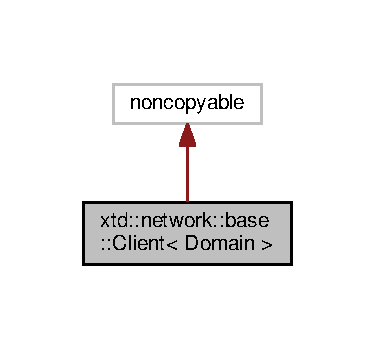
\includegraphics[width=180pt]{classxtd_1_1network_1_1base_1_1Client__inherit__graph}
\end{center}
\end{figure}


Collaboration diagram for xtd\-:\-:network\-:\-:base\-:\-:Client$<$ Domain $>$\-:
\nopagebreak
\begin{figure}[H]
\begin{center}
\leavevmode
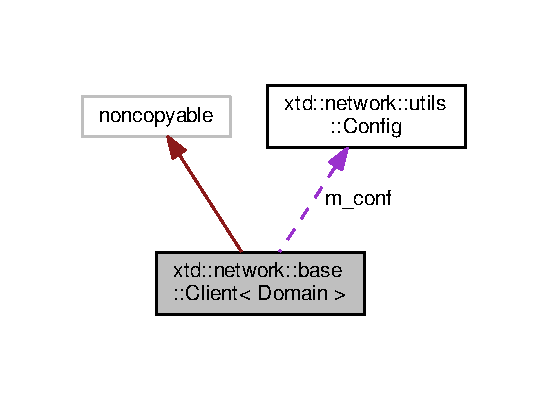
\includegraphics[width=263pt]{classxtd_1_1network_1_1base_1_1Client__coll__graph}
\end{center}
\end{figure}
\subsection*{Public Member Functions}
\begin{DoxyCompactItemize}
\item 
virtual \hyperlink{classxtd_1_1network_1_1base_1_1Client_a890cd6837ad0ccd2bf928f171e7696d0}{$\sim$\-Client} (void)
\item 
status \hyperlink{classxtd_1_1network_1_1base_1_1Client_abf9740f4b9eed341858ad27018cc4469}{connect} (const string \&p\-\_\-hostname, const uint32\-\_\-t p\-\_\-port)
\item 
void \hyperlink{classxtd_1_1network_1_1base_1_1Client_ac7427711e506f5958f80a89028f3f923}{async\-\_\-connect} (const string \&p\-\_\-hostname, const uint32\-\_\-t p\-\_\-port)
\item 
status \hyperlink{classxtd_1_1network_1_1base_1_1Client_ada6c4a1254620f7f5d83d3c890748300}{wait\-\_\-async\-\_\-connect} ()
\item 
status \hyperlink{classxtd_1_1network_1_1base_1_1Client_a268f40287ee277801cad202fa1380970}{reconnect} (void)
\item 
void \hyperlink{classxtd_1_1network_1_1base_1_1Client_a520d6aebfcf0e0892515bc0fec3a37c7}{close} (void)
\item 
const uint32\-\_\-t \& \hyperlink{classxtd_1_1network_1_1base_1_1Client_abff34ffec3663d843d97f42a7ce73d2f}{get\-Cnx\-Total} (void) const 
\item 
const uint32\-\_\-t \& \hyperlink{classxtd_1_1network_1_1base_1_1Client_a1d72f9e19322a7c2d533422c4f9e9777}{get\-Cnx\-Success} (void) const 
\item 
const uint32\-\_\-t \& \hyperlink{classxtd_1_1network_1_1base_1_1Client_aa585da9396b4067ac2535cdc4c1acbbb}{get\-Cnx\-Timeout} (void) const 
\item 
const uint32\-\_\-t \& \hyperlink{classxtd_1_1network_1_1base_1_1Client_a3023500754c12ccfdd200706d9995fd7}{get\-Cnx\-Error} (void) const 
\end{DoxyCompactItemize}
\subsection*{Protected Types}
\begin{DoxyCompactItemize}
\item 
typedef boost\-::shared\-\_\-ptr\\*
$<$ \hyperlink{classxtd_1_1network_1_1base_1_1Connection}{Connection}$<$ Domain $>$ $>$ \hyperlink{classxtd_1_1network_1_1base_1_1Client_a3cef8310676dac754d630bcc1628ab56}{cnx\-\_\-sptr\-\_\-t}
\end{DoxyCompactItemize}
\subsection*{Protected Member Functions}
\begin{DoxyCompactItemize}
\item 
\hyperlink{classxtd_1_1network_1_1base_1_1Client_a7afc6ed48caf877014df0a3128d6ed05}{Client} (const \hyperlink{classxtd_1_1network_1_1utils_1_1Config}{utils\-::\-Config} \&p\-\_\-conf)
\item 
virtual \hyperlink{classxtd_1_1network_1_1base_1_1Client_a3cef8310676dac754d630bcc1628ab56}{cnx\-\_\-sptr\-\_\-t} \hyperlink{classxtd_1_1network_1_1base_1_1Client_ad7964979939106d0c496c4f78a834b0d}{create\-Cnx} (string p\-\_\-hostname, uint32\-\_\-t p\-\_\-port)=0
\item 
virtual void \hyperlink{classxtd_1_1network_1_1base_1_1Client_a05ea029f4bfed5d9581ebc606e198336}{on\-Connected} (const boost\-::system\-::error\-\_\-code p\-\_\-error)
\end{DoxyCompactItemize}
\subsection*{Protected Attributes}
\begin{DoxyCompactItemize}
\item 
\hyperlink{classxtd_1_1network_1_1utils_1_1Config}{utils\-::\-Config} \hyperlink{classxtd_1_1network_1_1base_1_1Client_addb0f7fb40585d3db038b16f11e466cd}{m\-\_\-conf}
\item 
boost\-::asio\-::io\-\_\-service \& \hyperlink{classxtd_1_1network_1_1base_1_1Client_ae3945e4771a207872ab45b73de2e040f}{m\-\_\-io\-Service}
\item 
\hyperlink{classxtd_1_1network_1_1base_1_1Client_a3cef8310676dac754d630bcc1628ab56}{cnx\-\_\-sptr\-\_\-t} \hyperlink{classxtd_1_1network_1_1base_1_1Client_a9293a756af76e066790a1f389dbedb77}{m\-\_\-connection}
\item 
status \hyperlink{classxtd_1_1network_1_1base_1_1Client_a99e6d675c7617cd6d8e94793d8af4871}{m\-\_\-connect\-Status}
\end{DoxyCompactItemize}


\subsection{Detailed Description}
\subsubsection*{template$<$typename Domain$>$class xtd\-::network\-::base\-::\-Client$<$ Domain $>$}

T\-O\-D\-O explain private + shared\-\_\-ptr 

Definition at line 32 of file Client.\-hh.



\subsection{Member Typedef Documentation}
\hypertarget{classxtd_1_1network_1_1base_1_1Client_a3cef8310676dac754d630bcc1628ab56}{\index{xtd\-::network\-::base\-::\-Client@{xtd\-::network\-::base\-::\-Client}!cnx\-\_\-sptr\-\_\-t@{cnx\-\_\-sptr\-\_\-t}}
\index{cnx\-\_\-sptr\-\_\-t@{cnx\-\_\-sptr\-\_\-t}!xtd::network::base::Client@{xtd\-::network\-::base\-::\-Client}}
\subsubsection[{cnx\-\_\-sptr\-\_\-t}]{\setlength{\rightskip}{0pt plus 5cm}template$<$typename Domain$>$ typedef boost\-::shared\-\_\-ptr$<${\bf Connection}$<$Domain$>$ $>$ {\bf xtd\-::network\-::base\-::\-Client}$<$ Domain $>$\-::{\bf cnx\-\_\-sptr\-\_\-t}\hspace{0.3cm}{\ttfamily [protected]}}}\label{classxtd_1_1network_1_1base_1_1Client_a3cef8310676dac754d630bcc1628ab56}


Definition at line 35 of file Client.\-hh.



\subsection{Constructor \& Destructor Documentation}
\hypertarget{classxtd_1_1network_1_1base_1_1Client_a7afc6ed48caf877014df0a3128d6ed05}{\index{xtd\-::network\-::base\-::\-Client@{xtd\-::network\-::base\-::\-Client}!Client@{Client}}
\index{Client@{Client}!xtd::network::base::Client@{xtd\-::network\-::base\-::\-Client}}
\subsubsection[{Client}]{\setlength{\rightskip}{0pt plus 5cm}template$<$typename Domain$>$ {\bf xtd\-::network\-::base\-::\-Client}$<$ Domain $>$\-::{\bf Client} (
\begin{DoxyParamCaption}
\item[{const {\bf utils\-::\-Config} \&}]{p\-\_\-conf}
\end{DoxyParamCaption}
)\hspace{0.3cm}{\ttfamily [protected]}}}\label{classxtd_1_1network_1_1base_1_1Client_a7afc6ed48caf877014df0a3128d6ed05}
\hypertarget{classxtd_1_1network_1_1base_1_1Client_a890cd6837ad0ccd2bf928f171e7696d0}{\index{xtd\-::network\-::base\-::\-Client@{xtd\-::network\-::base\-::\-Client}!$\sim$\-Client@{$\sim$\-Client}}
\index{$\sim$\-Client@{$\sim$\-Client}!xtd::network::base::Client@{xtd\-::network\-::base\-::\-Client}}
\subsubsection[{$\sim$\-Client}]{\setlength{\rightskip}{0pt plus 5cm}template$<$typename Domain$>$ virtual {\bf xtd\-::network\-::base\-::\-Client}$<$ Domain $>$\-::$\sim${\bf Client} (
\begin{DoxyParamCaption}
\item[{void}]{}
\end{DoxyParamCaption}
)\hspace{0.3cm}{\ttfamily [virtual]}}}\label{classxtd_1_1network_1_1base_1_1Client_a890cd6837ad0ccd2bf928f171e7696d0}


Reimplemented in \hyperlink{classxtd_1_1network_1_1bip_1_1Client_ac16a5d30bae2e5ac5ae616034943d219}{xtd\-::network\-::bip\-::\-Client$<$ T\-Request, T\-Response, T\-Domain $>$}.



\subsection{Member Function Documentation}
\hypertarget{classxtd_1_1network_1_1base_1_1Client_ac7427711e506f5958f80a89028f3f923}{\index{xtd\-::network\-::base\-::\-Client@{xtd\-::network\-::base\-::\-Client}!async\-\_\-connect@{async\-\_\-connect}}
\index{async\-\_\-connect@{async\-\_\-connect}!xtd::network::base::Client@{xtd\-::network\-::base\-::\-Client}}
\subsubsection[{async\-\_\-connect}]{\setlength{\rightskip}{0pt plus 5cm}template$<$typename Domain$>$ void {\bf xtd\-::network\-::base\-::\-Client}$<$ Domain $>$\-::async\-\_\-connect (
\begin{DoxyParamCaption}
\item[{const string \&}]{p\-\_\-hostname, }
\item[{const uint32\-\_\-t}]{p\-\_\-port}
\end{DoxyParamCaption}
)}}\label{classxtd_1_1network_1_1base_1_1Client_ac7427711e506f5958f80a89028f3f923}
\hypertarget{classxtd_1_1network_1_1base_1_1Client_a520d6aebfcf0e0892515bc0fec3a37c7}{\index{xtd\-::network\-::base\-::\-Client@{xtd\-::network\-::base\-::\-Client}!close@{close}}
\index{close@{close}!xtd::network::base::Client@{xtd\-::network\-::base\-::\-Client}}
\subsubsection[{close}]{\setlength{\rightskip}{0pt plus 5cm}template$<$typename Domain$>$ void {\bf xtd\-::network\-::base\-::\-Client}$<$ Domain $>$\-::close (
\begin{DoxyParamCaption}
\item[{void}]{}
\end{DoxyParamCaption}
)}}\label{classxtd_1_1network_1_1base_1_1Client_a520d6aebfcf0e0892515bc0fec3a37c7}
\hypertarget{classxtd_1_1network_1_1base_1_1Client_abf9740f4b9eed341858ad27018cc4469}{\index{xtd\-::network\-::base\-::\-Client@{xtd\-::network\-::base\-::\-Client}!connect@{connect}}
\index{connect@{connect}!xtd::network::base::Client@{xtd\-::network\-::base\-::\-Client}}
\subsubsection[{connect}]{\setlength{\rightskip}{0pt plus 5cm}template$<$typename Domain$>$ status {\bf xtd\-::network\-::base\-::\-Client}$<$ Domain $>$\-::connect (
\begin{DoxyParamCaption}
\item[{const string \&}]{p\-\_\-hostname, }
\item[{const uint32\-\_\-t}]{p\-\_\-port}
\end{DoxyParamCaption}
)}}\label{classxtd_1_1network_1_1base_1_1Client_abf9740f4b9eed341858ad27018cc4469}
\hypertarget{classxtd_1_1network_1_1base_1_1Client_ad7964979939106d0c496c4f78a834b0d}{\index{xtd\-::network\-::base\-::\-Client@{xtd\-::network\-::base\-::\-Client}!create\-Cnx@{create\-Cnx}}
\index{create\-Cnx@{create\-Cnx}!xtd::network::base::Client@{xtd\-::network\-::base\-::\-Client}}
\subsubsection[{create\-Cnx}]{\setlength{\rightskip}{0pt plus 5cm}template$<$typename Domain$>$ virtual {\bf cnx\-\_\-sptr\-\_\-t} {\bf xtd\-::network\-::base\-::\-Client}$<$ Domain $>$\-::create\-Cnx (
\begin{DoxyParamCaption}
\item[{string}]{p\-\_\-hostname, }
\item[{uint32\-\_\-t}]{p\-\_\-port}
\end{DoxyParamCaption}
)\hspace{0.3cm}{\ttfamily [protected]}, {\ttfamily [pure virtual]}}}\label{classxtd_1_1network_1_1base_1_1Client_ad7964979939106d0c496c4f78a834b0d}
\hypertarget{classxtd_1_1network_1_1base_1_1Client_a3023500754c12ccfdd200706d9995fd7}{\index{xtd\-::network\-::base\-::\-Client@{xtd\-::network\-::base\-::\-Client}!get\-Cnx\-Error@{get\-Cnx\-Error}}
\index{get\-Cnx\-Error@{get\-Cnx\-Error}!xtd::network::base::Client@{xtd\-::network\-::base\-::\-Client}}
\subsubsection[{get\-Cnx\-Error}]{\setlength{\rightskip}{0pt plus 5cm}template$<$typename Domain$>$ const uint32\-\_\-t\& {\bf xtd\-::network\-::base\-::\-Client}$<$ Domain $>$\-::get\-Cnx\-Error (
\begin{DoxyParamCaption}
\item[{void}]{}
\end{DoxyParamCaption}
) const\hspace{0.3cm}{\ttfamily [inline]}}}\label{classxtd_1_1network_1_1base_1_1Client_a3023500754c12ccfdd200706d9995fd7}


Definition at line 56 of file Client.\-hh.


\begin{DoxyCode}
56 \{ \textcolor{keywordflow}{return} m\_cnxError; \}
\end{DoxyCode}
\hypertarget{classxtd_1_1network_1_1base_1_1Client_a1d72f9e19322a7c2d533422c4f9e9777}{\index{xtd\-::network\-::base\-::\-Client@{xtd\-::network\-::base\-::\-Client}!get\-Cnx\-Success@{get\-Cnx\-Success}}
\index{get\-Cnx\-Success@{get\-Cnx\-Success}!xtd::network::base::Client@{xtd\-::network\-::base\-::\-Client}}
\subsubsection[{get\-Cnx\-Success}]{\setlength{\rightskip}{0pt plus 5cm}template$<$typename Domain$>$ const uint32\-\_\-t\& {\bf xtd\-::network\-::base\-::\-Client}$<$ Domain $>$\-::get\-Cnx\-Success (
\begin{DoxyParamCaption}
\item[{void}]{}
\end{DoxyParamCaption}
) const\hspace{0.3cm}{\ttfamily [inline]}}}\label{classxtd_1_1network_1_1base_1_1Client_a1d72f9e19322a7c2d533422c4f9e9777}


Definition at line 54 of file Client.\-hh.


\begin{DoxyCode}
54 \{ \textcolor{keywordflow}{return} m\_cnxSuccess; \}
\end{DoxyCode}
\hypertarget{classxtd_1_1network_1_1base_1_1Client_aa585da9396b4067ac2535cdc4c1acbbb}{\index{xtd\-::network\-::base\-::\-Client@{xtd\-::network\-::base\-::\-Client}!get\-Cnx\-Timeout@{get\-Cnx\-Timeout}}
\index{get\-Cnx\-Timeout@{get\-Cnx\-Timeout}!xtd::network::base::Client@{xtd\-::network\-::base\-::\-Client}}
\subsubsection[{get\-Cnx\-Timeout}]{\setlength{\rightskip}{0pt plus 5cm}template$<$typename Domain$>$ const uint32\-\_\-t\& {\bf xtd\-::network\-::base\-::\-Client}$<$ Domain $>$\-::get\-Cnx\-Timeout (
\begin{DoxyParamCaption}
\item[{void}]{}
\end{DoxyParamCaption}
) const\hspace{0.3cm}{\ttfamily [inline]}}}\label{classxtd_1_1network_1_1base_1_1Client_aa585da9396b4067ac2535cdc4c1acbbb}


Definition at line 55 of file Client.\-hh.


\begin{DoxyCode}
55 \{ \textcolor{keywordflow}{return} m\_cnxTimeout; \}
\end{DoxyCode}
\hypertarget{classxtd_1_1network_1_1base_1_1Client_abff34ffec3663d843d97f42a7ce73d2f}{\index{xtd\-::network\-::base\-::\-Client@{xtd\-::network\-::base\-::\-Client}!get\-Cnx\-Total@{get\-Cnx\-Total}}
\index{get\-Cnx\-Total@{get\-Cnx\-Total}!xtd::network::base::Client@{xtd\-::network\-::base\-::\-Client}}
\subsubsection[{get\-Cnx\-Total}]{\setlength{\rightskip}{0pt plus 5cm}template$<$typename Domain$>$ const uint32\-\_\-t\& {\bf xtd\-::network\-::base\-::\-Client}$<$ Domain $>$\-::get\-Cnx\-Total (
\begin{DoxyParamCaption}
\item[{void}]{}
\end{DoxyParamCaption}
) const\hspace{0.3cm}{\ttfamily [inline]}}}\label{classxtd_1_1network_1_1base_1_1Client_abff34ffec3663d843d97f42a7ce73d2f}


Definition at line 53 of file Client.\-hh.


\begin{DoxyCode}
53 \{ \textcolor{keywordflow}{return} m\_cnxTotal; \}
\end{DoxyCode}
\hypertarget{classxtd_1_1network_1_1base_1_1Client_a05ea029f4bfed5d9581ebc606e198336}{\index{xtd\-::network\-::base\-::\-Client@{xtd\-::network\-::base\-::\-Client}!on\-Connected@{on\-Connected}}
\index{on\-Connected@{on\-Connected}!xtd::network::base::Client@{xtd\-::network\-::base\-::\-Client}}
\subsubsection[{on\-Connected}]{\setlength{\rightskip}{0pt plus 5cm}template$<$typename Domain$>$ virtual void {\bf xtd\-::network\-::base\-::\-Client}$<$ Domain $>$\-::on\-Connected (
\begin{DoxyParamCaption}
\item[{const boost\-::system\-::error\-\_\-code}]{p\-\_\-error}
\end{DoxyParamCaption}
)\hspace{0.3cm}{\ttfamily [protected]}, {\ttfamily [virtual]}}}\label{classxtd_1_1network_1_1base_1_1Client_a05ea029f4bfed5d9581ebc606e198336}
\hypertarget{classxtd_1_1network_1_1base_1_1Client_a268f40287ee277801cad202fa1380970}{\index{xtd\-::network\-::base\-::\-Client@{xtd\-::network\-::base\-::\-Client}!reconnect@{reconnect}}
\index{reconnect@{reconnect}!xtd::network::base::Client@{xtd\-::network\-::base\-::\-Client}}
\subsubsection[{reconnect}]{\setlength{\rightskip}{0pt plus 5cm}template$<$typename Domain$>$ status {\bf xtd\-::network\-::base\-::\-Client}$<$ Domain $>$\-::reconnect (
\begin{DoxyParamCaption}
\item[{void}]{}
\end{DoxyParamCaption}
)}}\label{classxtd_1_1network_1_1base_1_1Client_a268f40287ee277801cad202fa1380970}
\hypertarget{classxtd_1_1network_1_1base_1_1Client_ada6c4a1254620f7f5d83d3c890748300}{\index{xtd\-::network\-::base\-::\-Client@{xtd\-::network\-::base\-::\-Client}!wait\-\_\-async\-\_\-connect@{wait\-\_\-async\-\_\-connect}}
\index{wait\-\_\-async\-\_\-connect@{wait\-\_\-async\-\_\-connect}!xtd::network::base::Client@{xtd\-::network\-::base\-::\-Client}}
\subsubsection[{wait\-\_\-async\-\_\-connect}]{\setlength{\rightskip}{0pt plus 5cm}template$<$typename Domain$>$ status {\bf xtd\-::network\-::base\-::\-Client}$<$ Domain $>$\-::wait\-\_\-async\-\_\-connect (
\begin{DoxyParamCaption}
{}
\end{DoxyParamCaption}
)}}\label{classxtd_1_1network_1_1base_1_1Client_ada6c4a1254620f7f5d83d3c890748300}


\subsection{Member Data Documentation}
\hypertarget{classxtd_1_1network_1_1base_1_1Client_addb0f7fb40585d3db038b16f11e466cd}{\index{xtd\-::network\-::base\-::\-Client@{xtd\-::network\-::base\-::\-Client}!m\-\_\-conf@{m\-\_\-conf}}
\index{m\-\_\-conf@{m\-\_\-conf}!xtd::network::base::Client@{xtd\-::network\-::base\-::\-Client}}
\subsubsection[{m\-\_\-conf}]{\setlength{\rightskip}{0pt plus 5cm}template$<$typename Domain$>$ {\bf utils\-::\-Config} {\bf xtd\-::network\-::base\-::\-Client}$<$ Domain $>$\-::m\-\_\-conf\hspace{0.3cm}{\ttfamily [protected]}}}\label{classxtd_1_1network_1_1base_1_1Client_addb0f7fb40585d3db038b16f11e466cd}


Definition at line 70 of file Client.\-hh.

\hypertarget{classxtd_1_1network_1_1base_1_1Client_a9293a756af76e066790a1f389dbedb77}{\index{xtd\-::network\-::base\-::\-Client@{xtd\-::network\-::base\-::\-Client}!m\-\_\-connection@{m\-\_\-connection}}
\index{m\-\_\-connection@{m\-\_\-connection}!xtd::network::base::Client@{xtd\-::network\-::base\-::\-Client}}
\subsubsection[{m\-\_\-connection}]{\setlength{\rightskip}{0pt plus 5cm}template$<$typename Domain$>$ {\bf cnx\-\_\-sptr\-\_\-t} {\bf xtd\-::network\-::base\-::\-Client}$<$ Domain $>$\-::m\-\_\-connection\hspace{0.3cm}{\ttfamily [protected]}}}\label{classxtd_1_1network_1_1base_1_1Client_a9293a756af76e066790a1f389dbedb77}


Definition at line 72 of file Client.\-hh.

\hypertarget{classxtd_1_1network_1_1base_1_1Client_a99e6d675c7617cd6d8e94793d8af4871}{\index{xtd\-::network\-::base\-::\-Client@{xtd\-::network\-::base\-::\-Client}!m\-\_\-connect\-Status@{m\-\_\-connect\-Status}}
\index{m\-\_\-connect\-Status@{m\-\_\-connect\-Status}!xtd::network::base::Client@{xtd\-::network\-::base\-::\-Client}}
\subsubsection[{m\-\_\-connect\-Status}]{\setlength{\rightskip}{0pt plus 5cm}template$<$typename Domain$>$ status {\bf xtd\-::network\-::base\-::\-Client}$<$ Domain $>$\-::m\-\_\-connect\-Status\hspace{0.3cm}{\ttfamily [protected]}}}\label{classxtd_1_1network_1_1base_1_1Client_a99e6d675c7617cd6d8e94793d8af4871}


Definition at line 73 of file Client.\-hh.

\hypertarget{classxtd_1_1network_1_1base_1_1Client_ae3945e4771a207872ab45b73de2e040f}{\index{xtd\-::network\-::base\-::\-Client@{xtd\-::network\-::base\-::\-Client}!m\-\_\-io\-Service@{m\-\_\-io\-Service}}
\index{m\-\_\-io\-Service@{m\-\_\-io\-Service}!xtd::network::base::Client@{xtd\-::network\-::base\-::\-Client}}
\subsubsection[{m\-\_\-io\-Service}]{\setlength{\rightskip}{0pt plus 5cm}template$<$typename Domain$>$ boost\-::asio\-::io\-\_\-service\& {\bf xtd\-::network\-::base\-::\-Client}$<$ Domain $>$\-::m\-\_\-io\-Service\hspace{0.3cm}{\ttfamily [protected]}}}\label{classxtd_1_1network_1_1base_1_1Client_ae3945e4771a207872ab45b73de2e040f}


Definition at line 71 of file Client.\-hh.



The documentation for this class was generated from the following file\-:\begin{DoxyCompactItemize}
\item 
/home/travis/build/psycofdj/xtdcpp/network/src/base/\hyperlink{base_2Client_8hh}{Client.\-hh}\end{DoxyCompactItemize}

\hypertarget{classxtd_1_1network_1_1bip_1_1Client}{}\section{xtd\+:\+:network\+:\+:bip\+:\+:Client$<$ T\+Request, T\+Response, T\+Domain $>$ Class Template Reference}
\label{classxtd_1_1network_1_1bip_1_1Client}\index{xtd\+::network\+::bip\+::\+Client$<$ T\+Request, T\+Response, T\+Domain $>$@{xtd\+::network\+::bip\+::\+Client$<$ T\+Request, T\+Response, T\+Domain $>$}}


{\ttfamily \#include $<$Client.\+hh$>$}



Inheritance diagram for xtd\+:\+:network\+:\+:bip\+:\+:Client$<$ T\+Request, T\+Response, T\+Domain $>$\+:
\nopagebreak
\begin{figure}[H]
\begin{center}
\leavevmode
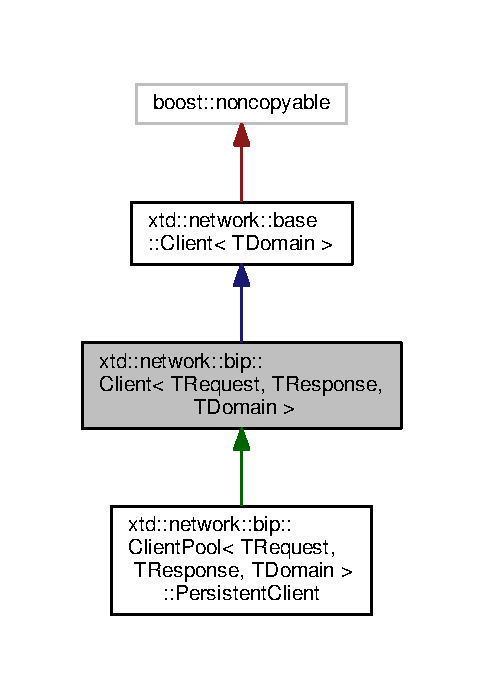
\includegraphics[width=233pt]{classxtd_1_1network_1_1bip_1_1Client__inherit__graph}
\end{center}
\end{figure}


Collaboration diagram for xtd\+:\+:network\+:\+:bip\+:\+:Client$<$ T\+Request, T\+Response, T\+Domain $>$\+:
\nopagebreak
\begin{figure}[H]
\begin{center}
\leavevmode
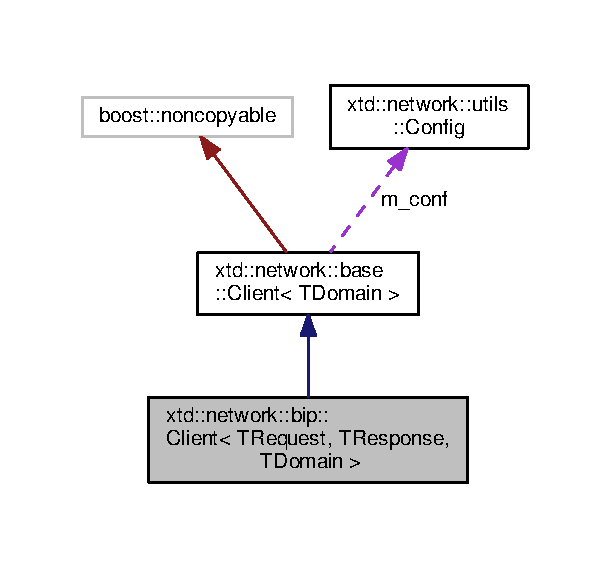
\includegraphics[width=294pt]{classxtd_1_1network_1_1bip_1_1Client__coll__graph}
\end{center}
\end{figure}
\subsection*{Public Types}
\begin{DoxyCompactItemize}
\item 
typedef T\+Request \hyperlink{classxtd_1_1network_1_1bip_1_1Client_a4fd207d42e4738c5aa2f6ca947067be4}{T\+Req}
\item 
typedef T\+Response \hyperlink{classxtd_1_1network_1_1bip_1_1Client_a1fc57254a811008a795987c49c222e77}{T\+Res}
\end{DoxyCompactItemize}
\subsection*{Public Member Functions}
\begin{DoxyCompactItemize}
\item 
\hyperlink{classxtd_1_1network_1_1bip_1_1Client_a49c9e08bee4169c40c92d9870d882295}{Client} (const \hyperlink{classxtd_1_1network_1_1utils_1_1Config}{utils\+::\+Config} \&p\+\_\+conf)
\item 
virtual \hyperlink{classxtd_1_1network_1_1bip_1_1Client_ac16a5d30bae2e5ac5ae616034943d219}{$\sim$\+Client} (void)
\item 
const uint32\+\_\+t \& \hyperlink{classxtd_1_1network_1_1bip_1_1Client_ad9097285a9937b9b16922ea3f5154cd2}{get\+Send\+Total} (void) const 
\item 
const uint32\+\_\+t \& \hyperlink{classxtd_1_1network_1_1bip_1_1Client_ae0112d61b8a18823bffb8c7b3bde9b4d}{get\+Send\+Success} (void) const 
\item 
const uint32\+\_\+t \& \hyperlink{classxtd_1_1network_1_1bip_1_1Client_ad7b29723945a80df67837c41b4570272}{get\+Send\+Timeout} (void) const 
\item 
const uint32\+\_\+t \& \hyperlink{classxtd_1_1network_1_1bip_1_1Client_afa332d8733f5a96b85546de8dc37dffc}{get\+Send\+Error} (void) const 
\item 
const uint32\+\_\+t \& \hyperlink{classxtd_1_1network_1_1bip_1_1Client_af8c4e73103c9e483f78c9b62496daf47}{get\+Receive\+Total} (void) const 
\item 
const uint32\+\_\+t \& \hyperlink{classxtd_1_1network_1_1bip_1_1Client_a7fb2624e39723bae24d8286b98795e70}{get\+Receive\+Success} (void) const 
\item 
const uint32\+\_\+t \& \hyperlink{classxtd_1_1network_1_1bip_1_1Client_adfcc8fafdf138d104d78133ff5f419df}{get\+Receive\+Timeout} (void) const 
\item 
const uint32\+\_\+t \& \hyperlink{classxtd_1_1network_1_1bip_1_1Client_ab04f56d8e2cb6ac3d7fdaa2e1791c7cd}{get\+Receive\+Error} (void) const 
\item 
const uint32\+\_\+t \& \hyperlink{classxtd_1_1network_1_1bip_1_1Client_a44ee99fff5318cdd6e6b54b4b5e2f62f}{get\+Last\+R\+T\+T\+Ms} (void) const 
\item 
status \hyperlink{classxtd_1_1network_1_1bip_1_1Client_acda47c19d4fc71705f4db91226cec1b9}{send} (const T\+Request \&p\+\_\+request, bool p\+\_\+debug)
\begin{DoxyCompactList}\small\item\em envoi d\textquotesingle{}une structure requête au server \end{DoxyCompactList}\item 
status \hyperlink{classxtd_1_1network_1_1bip_1_1Client_a0e259e8174324fdbc199eb87427aa237}{receive} (T\+Response \&p\+\_\+response, bool \&p\+\_\+debug)
\begin{DoxyCompactList}\small\item\em reception de la structure réponse \end{DoxyCompactList}\item 
virtual bool \hyperlink{classxtd_1_1network_1_1bip_1_1Client_a5721e7ec64739ab5a252d5ac59e4a86e}{should\+Receive} (const T\+Request \&p\+\_\+request, const bool p\+\_\+request\+Debug)
\end{DoxyCompactItemize}
\subsection*{Additional Inherited Members}


\subsection{Detailed Description}
\subsubsection*{template$<$class T\+Request, class T\+Response, typename T\+Domain = utils\+::af\+\_\+inet$>$\\*
class xtd\+::network\+::bip\+::\+Client$<$ T\+Request, T\+Response, T\+Domain $>$}


\begin{DoxyParams}{Parameters}
{\em T\+Domain} & \+: mode de connexion, \hyperlink{namespacextd_1_1network_1_1utils_a6238bab7a616eda8c9424721444a18d1}{utils\+::af\+\_\+inet} ou \hyperlink{namespacextd_1_1network_1_1utils_a60e83921a2d026f07b49fa094988acdf}{utils\+::af\+\_\+unix} \\
\hline
{\em T\+Request} & Structure requète serialisable avec boost\+::serialization \\
\hline
{\em T\+Response} & Structure réponse serialisable avec boost\+::serialization\\
\hline
\end{DoxyParams}
\hyperlink{classxtd_1_1network_1_1bip_1_1Client}{Client} générique bip \+: gère l\textquotesingle{}envoi de structure T\+Request et la réception de structure T\+Response vers un serveur bip de même type.

Selon la configuration transmise au constructeur, les données pourront etre compressées avant l\textquotesingle{}envoi et décompressée à la réception.

La méthode send de cet objet est non bloquante et déclenche, en interne, la réception de la réponse du serveur. La méthode receive, elle, est bloquante jusqu\textquotesingle{}à la réception effective de la réponse. Cette approche permet à un utilisateur, qui aurait plusieurs client connectés vers plusieurs serveurs, d\textquotesingle{}envoyer ses requètes et de réceptionner en parallèle ses réponses pour au final aller au rythme du serveur le plus lent et pas subir la somme de tous les temps de réponse.

Thread safety \+:
\begin{DoxyItemize}
\item même instance \+: non
\item instances différentes \+: oui 
\end{DoxyItemize}

Definition at line 35 of file Client.\+hh.



\subsection{Member Typedef Documentation}
\index{xtd\+::network\+::bip\+::\+Client@{xtd\+::network\+::bip\+::\+Client}!T\+Req@{T\+Req}}
\index{T\+Req@{T\+Req}!xtd\+::network\+::bip\+::\+Client@{xtd\+::network\+::bip\+::\+Client}}
\subsubsection[{\texorpdfstring{T\+Req}{TReq}}]{\setlength{\rightskip}{0pt plus 5cm}template$<$class T\+Request , class T\+Response , typename T\+Domain  = utils\+::af\+\_\+inet$>$ typedef T\+Request {\bf xtd\+::network\+::bip\+::\+Client}$<$ T\+Request, T\+Response, T\+Domain $>$\+::{\bf T\+Req}}\hypertarget{classxtd_1_1network_1_1bip_1_1Client_a4fd207d42e4738c5aa2f6ca947067be4}{}\label{classxtd_1_1network_1_1bip_1_1Client_a4fd207d42e4738c5aa2f6ca947067be4}


Definition at line 38 of file Client.\+hh.

\index{xtd\+::network\+::bip\+::\+Client@{xtd\+::network\+::bip\+::\+Client}!T\+Res@{T\+Res}}
\index{T\+Res@{T\+Res}!xtd\+::network\+::bip\+::\+Client@{xtd\+::network\+::bip\+::\+Client}}
\subsubsection[{\texorpdfstring{T\+Res}{TRes}}]{\setlength{\rightskip}{0pt plus 5cm}template$<$class T\+Request , class T\+Response , typename T\+Domain  = utils\+::af\+\_\+inet$>$ typedef T\+Response {\bf xtd\+::network\+::bip\+::\+Client}$<$ T\+Request, T\+Response, T\+Domain $>$\+::{\bf T\+Res}}\hypertarget{classxtd_1_1network_1_1bip_1_1Client_a1fc57254a811008a795987c49c222e77}{}\label{classxtd_1_1network_1_1bip_1_1Client_a1fc57254a811008a795987c49c222e77}


Definition at line 39 of file Client.\+hh.



\subsection{Constructor \& Destructor Documentation}
\index{xtd\+::network\+::bip\+::\+Client@{xtd\+::network\+::bip\+::\+Client}!Client@{Client}}
\index{Client@{Client}!xtd\+::network\+::bip\+::\+Client@{xtd\+::network\+::bip\+::\+Client}}
\subsubsection[{\texorpdfstring{Client(const utils\+::\+Config \&p\+\_\+conf)}{Client(const utils::Config &p_conf)}}]{\setlength{\rightskip}{0pt plus 5cm}template$<$class T\+Request , class T\+Response , typename T\+Domain  = utils\+::af\+\_\+inet$>$ {\bf xtd\+::network\+::bip\+::\+Client}$<$ T\+Request, T\+Response, T\+Domain $>$\+::{\bf Client} (
\begin{DoxyParamCaption}
\item[{const {\bf utils\+::\+Config} \&}]{p\+\_\+conf}
\end{DoxyParamCaption}
)}\hypertarget{classxtd_1_1network_1_1bip_1_1Client_a49c9e08bee4169c40c92d9870d882295}{}\label{classxtd_1_1network_1_1bip_1_1Client_a49c9e08bee4169c40c92d9870d882295}
\index{xtd\+::network\+::bip\+::\+Client@{xtd\+::network\+::bip\+::\+Client}!````~Client@{$\sim$\+Client}}
\index{````~Client@{$\sim$\+Client}!xtd\+::network\+::bip\+::\+Client@{xtd\+::network\+::bip\+::\+Client}}
\subsubsection[{\texorpdfstring{$\sim$\+Client(void)}{~Client(void)}}]{\setlength{\rightskip}{0pt plus 5cm}template$<$class T\+Request , class T\+Response , typename T\+Domain  = utils\+::af\+\_\+inet$>$ virtual {\bf xtd\+::network\+::bip\+::\+Client}$<$ T\+Request, T\+Response, T\+Domain $>$\+::$\sim${\bf Client} (
\begin{DoxyParamCaption}
\item[{void}]{}
\end{DoxyParamCaption}
)\hspace{0.3cm}{\ttfamily [virtual]}}\hypertarget{classxtd_1_1network_1_1bip_1_1Client_ac16a5d30bae2e5ac5ae616034943d219}{}\label{classxtd_1_1network_1_1bip_1_1Client_ac16a5d30bae2e5ac5ae616034943d219}


Reimplemented from \hyperlink{classxtd_1_1network_1_1base_1_1Client_a890cd6837ad0ccd2bf928f171e7696d0}{xtd\+::network\+::base\+::\+Client$<$ T\+Domain $>$}.



\subsection{Member Function Documentation}
\index{xtd\+::network\+::bip\+::\+Client@{xtd\+::network\+::bip\+::\+Client}!get\+Last\+R\+T\+T\+Ms@{get\+Last\+R\+T\+T\+Ms}}
\index{get\+Last\+R\+T\+T\+Ms@{get\+Last\+R\+T\+T\+Ms}!xtd\+::network\+::bip\+::\+Client@{xtd\+::network\+::bip\+::\+Client}}
\subsubsection[{\texorpdfstring{get\+Last\+R\+T\+T\+Ms(void) const }{getLastRTTMs(void) const }}]{\setlength{\rightskip}{0pt plus 5cm}template$<$class T\+Request , class T\+Response , typename T\+Domain  = utils\+::af\+\_\+inet$>$ const uint32\+\_\+t\& {\bf xtd\+::network\+::bip\+::\+Client}$<$ T\+Request, T\+Response, T\+Domain $>$\+::get\+Last\+R\+T\+T\+Ms (
\begin{DoxyParamCaption}
\item[{void}]{}
\end{DoxyParamCaption}
) const\hspace{0.3cm}{\ttfamily [inline]}}\hypertarget{classxtd_1_1network_1_1bip_1_1Client_a44ee99fff5318cdd6e6b54b4b5e2f62f}{}\label{classxtd_1_1network_1_1bip_1_1Client_a44ee99fff5318cdd6e6b54b4b5e2f62f}


Definition at line 71 of file Client.\+hh.


\begin{DoxyCode}
71 \{ \textcolor{keywordflow}{return} m\_lastRTTMs; \}
\end{DoxyCode}


Here is the call graph for this function\+:
\nopagebreak
\begin{figure}[H]
\begin{center}
\leavevmode
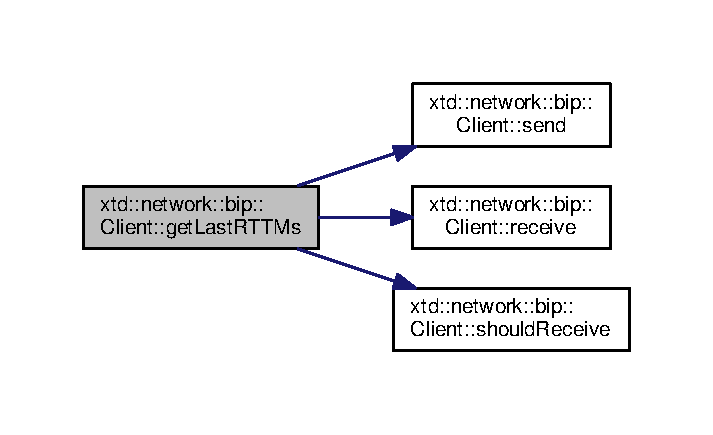
\includegraphics[width=342pt]{classxtd_1_1network_1_1bip_1_1Client_a44ee99fff5318cdd6e6b54b4b5e2f62f_cgraph}
\end{center}
\end{figure}


\index{xtd\+::network\+::bip\+::\+Client@{xtd\+::network\+::bip\+::\+Client}!get\+Receive\+Error@{get\+Receive\+Error}}
\index{get\+Receive\+Error@{get\+Receive\+Error}!xtd\+::network\+::bip\+::\+Client@{xtd\+::network\+::bip\+::\+Client}}
\subsubsection[{\texorpdfstring{get\+Receive\+Error(void) const }{getReceiveError(void) const }}]{\setlength{\rightskip}{0pt plus 5cm}template$<$class T\+Request , class T\+Response , typename T\+Domain  = utils\+::af\+\_\+inet$>$ const uint32\+\_\+t\& {\bf xtd\+::network\+::bip\+::\+Client}$<$ T\+Request, T\+Response, T\+Domain $>$\+::get\+Receive\+Error (
\begin{DoxyParamCaption}
\item[{void}]{}
\end{DoxyParamCaption}
) const\hspace{0.3cm}{\ttfamily [inline]}}\hypertarget{classxtd_1_1network_1_1bip_1_1Client_ab04f56d8e2cb6ac3d7fdaa2e1791c7cd}{}\label{classxtd_1_1network_1_1bip_1_1Client_ab04f56d8e2cb6ac3d7fdaa2e1791c7cd}


Definition at line 70 of file Client.\+hh.


\begin{DoxyCode}
70 \{ \textcolor{keywordflow}{return} m\_receiveError; \}
\end{DoxyCode}
\index{xtd\+::network\+::bip\+::\+Client@{xtd\+::network\+::bip\+::\+Client}!get\+Receive\+Success@{get\+Receive\+Success}}
\index{get\+Receive\+Success@{get\+Receive\+Success}!xtd\+::network\+::bip\+::\+Client@{xtd\+::network\+::bip\+::\+Client}}
\subsubsection[{\texorpdfstring{get\+Receive\+Success(void) const }{getReceiveSuccess(void) const }}]{\setlength{\rightskip}{0pt plus 5cm}template$<$class T\+Request , class T\+Response , typename T\+Domain  = utils\+::af\+\_\+inet$>$ const uint32\+\_\+t\& {\bf xtd\+::network\+::bip\+::\+Client}$<$ T\+Request, T\+Response, T\+Domain $>$\+::get\+Receive\+Success (
\begin{DoxyParamCaption}
\item[{void}]{}
\end{DoxyParamCaption}
) const\hspace{0.3cm}{\ttfamily [inline]}}\hypertarget{classxtd_1_1network_1_1bip_1_1Client_a7fb2624e39723bae24d8286b98795e70}{}\label{classxtd_1_1network_1_1bip_1_1Client_a7fb2624e39723bae24d8286b98795e70}


Definition at line 68 of file Client.\+hh.


\begin{DoxyCode}
68 \{ \textcolor{keywordflow}{return} m\_receiveSuccess; \}
\end{DoxyCode}
\index{xtd\+::network\+::bip\+::\+Client@{xtd\+::network\+::bip\+::\+Client}!get\+Receive\+Timeout@{get\+Receive\+Timeout}}
\index{get\+Receive\+Timeout@{get\+Receive\+Timeout}!xtd\+::network\+::bip\+::\+Client@{xtd\+::network\+::bip\+::\+Client}}
\subsubsection[{\texorpdfstring{get\+Receive\+Timeout(void) const }{getReceiveTimeout(void) const }}]{\setlength{\rightskip}{0pt plus 5cm}template$<$class T\+Request , class T\+Response , typename T\+Domain  = utils\+::af\+\_\+inet$>$ const uint32\+\_\+t\& {\bf xtd\+::network\+::bip\+::\+Client}$<$ T\+Request, T\+Response, T\+Domain $>$\+::get\+Receive\+Timeout (
\begin{DoxyParamCaption}
\item[{void}]{}
\end{DoxyParamCaption}
) const\hspace{0.3cm}{\ttfamily [inline]}}\hypertarget{classxtd_1_1network_1_1bip_1_1Client_adfcc8fafdf138d104d78133ff5f419df}{}\label{classxtd_1_1network_1_1bip_1_1Client_adfcc8fafdf138d104d78133ff5f419df}


Definition at line 69 of file Client.\+hh.


\begin{DoxyCode}
69 \{ \textcolor{keywordflow}{return} m\_receiveTimeout; \}
\end{DoxyCode}
\index{xtd\+::network\+::bip\+::\+Client@{xtd\+::network\+::bip\+::\+Client}!get\+Receive\+Total@{get\+Receive\+Total}}
\index{get\+Receive\+Total@{get\+Receive\+Total}!xtd\+::network\+::bip\+::\+Client@{xtd\+::network\+::bip\+::\+Client}}
\subsubsection[{\texorpdfstring{get\+Receive\+Total(void) const }{getReceiveTotal(void) const }}]{\setlength{\rightskip}{0pt plus 5cm}template$<$class T\+Request , class T\+Response , typename T\+Domain  = utils\+::af\+\_\+inet$>$ const uint32\+\_\+t\& {\bf xtd\+::network\+::bip\+::\+Client}$<$ T\+Request, T\+Response, T\+Domain $>$\+::get\+Receive\+Total (
\begin{DoxyParamCaption}
\item[{void}]{}
\end{DoxyParamCaption}
) const\hspace{0.3cm}{\ttfamily [inline]}}\hypertarget{classxtd_1_1network_1_1bip_1_1Client_af8c4e73103c9e483f78c9b62496daf47}{}\label{classxtd_1_1network_1_1bip_1_1Client_af8c4e73103c9e483f78c9b62496daf47}


Definition at line 67 of file Client.\+hh.


\begin{DoxyCode}
67 \{ \textcolor{keywordflow}{return} m\_receiveTotal; \}
\end{DoxyCode}
\index{xtd\+::network\+::bip\+::\+Client@{xtd\+::network\+::bip\+::\+Client}!get\+Send\+Error@{get\+Send\+Error}}
\index{get\+Send\+Error@{get\+Send\+Error}!xtd\+::network\+::bip\+::\+Client@{xtd\+::network\+::bip\+::\+Client}}
\subsubsection[{\texorpdfstring{get\+Send\+Error(void) const }{getSendError(void) const }}]{\setlength{\rightskip}{0pt plus 5cm}template$<$class T\+Request , class T\+Response , typename T\+Domain  = utils\+::af\+\_\+inet$>$ const uint32\+\_\+t\& {\bf xtd\+::network\+::bip\+::\+Client}$<$ T\+Request, T\+Response, T\+Domain $>$\+::get\+Send\+Error (
\begin{DoxyParamCaption}
\item[{void}]{}
\end{DoxyParamCaption}
) const\hspace{0.3cm}{\ttfamily [inline]}}\hypertarget{classxtd_1_1network_1_1bip_1_1Client_afa332d8733f5a96b85546de8dc37dffc}{}\label{classxtd_1_1network_1_1bip_1_1Client_afa332d8733f5a96b85546de8dc37dffc}


Definition at line 66 of file Client.\+hh.


\begin{DoxyCode}
66 \{ \textcolor{keywordflow}{return} m\_sendError; \}
\end{DoxyCode}
\index{xtd\+::network\+::bip\+::\+Client@{xtd\+::network\+::bip\+::\+Client}!get\+Send\+Success@{get\+Send\+Success}}
\index{get\+Send\+Success@{get\+Send\+Success}!xtd\+::network\+::bip\+::\+Client@{xtd\+::network\+::bip\+::\+Client}}
\subsubsection[{\texorpdfstring{get\+Send\+Success(void) const }{getSendSuccess(void) const }}]{\setlength{\rightskip}{0pt plus 5cm}template$<$class T\+Request , class T\+Response , typename T\+Domain  = utils\+::af\+\_\+inet$>$ const uint32\+\_\+t\& {\bf xtd\+::network\+::bip\+::\+Client}$<$ T\+Request, T\+Response, T\+Domain $>$\+::get\+Send\+Success (
\begin{DoxyParamCaption}
\item[{void}]{}
\end{DoxyParamCaption}
) const\hspace{0.3cm}{\ttfamily [inline]}}\hypertarget{classxtd_1_1network_1_1bip_1_1Client_ae0112d61b8a18823bffb8c7b3bde9b4d}{}\label{classxtd_1_1network_1_1bip_1_1Client_ae0112d61b8a18823bffb8c7b3bde9b4d}


Definition at line 64 of file Client.\+hh.


\begin{DoxyCode}
64 \{ \textcolor{keywordflow}{return} m\_sendSuccess; \}
\end{DoxyCode}
\index{xtd\+::network\+::bip\+::\+Client@{xtd\+::network\+::bip\+::\+Client}!get\+Send\+Timeout@{get\+Send\+Timeout}}
\index{get\+Send\+Timeout@{get\+Send\+Timeout}!xtd\+::network\+::bip\+::\+Client@{xtd\+::network\+::bip\+::\+Client}}
\subsubsection[{\texorpdfstring{get\+Send\+Timeout(void) const }{getSendTimeout(void) const }}]{\setlength{\rightskip}{0pt plus 5cm}template$<$class T\+Request , class T\+Response , typename T\+Domain  = utils\+::af\+\_\+inet$>$ const uint32\+\_\+t\& {\bf xtd\+::network\+::bip\+::\+Client}$<$ T\+Request, T\+Response, T\+Domain $>$\+::get\+Send\+Timeout (
\begin{DoxyParamCaption}
\item[{void}]{}
\end{DoxyParamCaption}
) const\hspace{0.3cm}{\ttfamily [inline]}}\hypertarget{classxtd_1_1network_1_1bip_1_1Client_ad7b29723945a80df67837c41b4570272}{}\label{classxtd_1_1network_1_1bip_1_1Client_ad7b29723945a80df67837c41b4570272}


Definition at line 65 of file Client.\+hh.


\begin{DoxyCode}
65 \{ \textcolor{keywordflow}{return} m\_sendTimeout; \}
\end{DoxyCode}
\index{xtd\+::network\+::bip\+::\+Client@{xtd\+::network\+::bip\+::\+Client}!get\+Send\+Total@{get\+Send\+Total}}
\index{get\+Send\+Total@{get\+Send\+Total}!xtd\+::network\+::bip\+::\+Client@{xtd\+::network\+::bip\+::\+Client}}
\subsubsection[{\texorpdfstring{get\+Send\+Total(void) const }{getSendTotal(void) const }}]{\setlength{\rightskip}{0pt plus 5cm}template$<$class T\+Request , class T\+Response , typename T\+Domain  = utils\+::af\+\_\+inet$>$ const uint32\+\_\+t\& {\bf xtd\+::network\+::bip\+::\+Client}$<$ T\+Request, T\+Response, T\+Domain $>$\+::get\+Send\+Total (
\begin{DoxyParamCaption}
\item[{void}]{}
\end{DoxyParamCaption}
) const\hspace{0.3cm}{\ttfamily [inline]}}\hypertarget{classxtd_1_1network_1_1bip_1_1Client_ad9097285a9937b9b16922ea3f5154cd2}{}\label{classxtd_1_1network_1_1bip_1_1Client_ad9097285a9937b9b16922ea3f5154cd2}


Definition at line 63 of file Client.\+hh.


\begin{DoxyCode}
63 \{ \textcolor{keywordflow}{return} m\_sendTotal; \}
\end{DoxyCode}
\index{xtd\+::network\+::bip\+::\+Client@{xtd\+::network\+::bip\+::\+Client}!receive@{receive}}
\index{receive@{receive}!xtd\+::network\+::bip\+::\+Client@{xtd\+::network\+::bip\+::\+Client}}
\subsubsection[{\texorpdfstring{receive(\+T\+Response \&p\+\_\+response, bool \&p\+\_\+debug)}{receive(TResponse &p_response, bool &p_debug)}}]{\setlength{\rightskip}{0pt plus 5cm}template$<$class T\+Request , class T\+Response , typename T\+Domain  = utils\+::af\+\_\+inet$>$ status {\bf xtd\+::network\+::bip\+::\+Client}$<$ T\+Request, T\+Response, T\+Domain $>$\+::receive (
\begin{DoxyParamCaption}
\item[{T\+Response \&}]{p\+\_\+response, }
\item[{bool \&}]{p\+\_\+debug}
\end{DoxyParamCaption}
)}\hypertarget{classxtd_1_1network_1_1bip_1_1Client_a0e259e8174324fdbc199eb87427aa237}{}\label{classxtd_1_1network_1_1bip_1_1Client_a0e259e8174324fdbc199eb87427aa237}


reception de la structure réponse 


\begin{DoxyParams}{Parameters}
{\em p\+\_\+response} & structure à remplir avec la réponse du server \\
\hline
{\em p\+\_\+debug} & sortira à la valeur true si le serveur a envoyé la partie débug de la structure \\
\hline
\end{DoxyParams}
\begin{DoxyReturn}{Returns}
status\+::ok si tout va bien, status\+::timeout en cas de timeout et staus\+::error en cas d\textquotesingle{}erreur.
\end{DoxyReturn}
Cette méthode est bloquante, elle attend la réception effective de la réponse du serveur ou la survenue d\textquotesingle{}une erreur/timeout. 

Here is the caller graph for this function\+:
\nopagebreak
\begin{figure}[H]
\begin{center}
\leavevmode
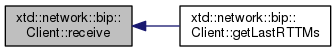
\includegraphics[width=324pt]{classxtd_1_1network_1_1bip_1_1Client_a0e259e8174324fdbc199eb87427aa237_icgraph}
\end{center}
\end{figure}


\index{xtd\+::network\+::bip\+::\+Client@{xtd\+::network\+::bip\+::\+Client}!send@{send}}
\index{send@{send}!xtd\+::network\+::bip\+::\+Client@{xtd\+::network\+::bip\+::\+Client}}
\subsubsection[{\texorpdfstring{send(const T\+Request \&p\+\_\+request, bool p\+\_\+debug)}{send(const TRequest &p_request, bool p_debug)}}]{\setlength{\rightskip}{0pt plus 5cm}template$<$class T\+Request , class T\+Response , typename T\+Domain  = utils\+::af\+\_\+inet$>$ status {\bf xtd\+::network\+::bip\+::\+Client}$<$ T\+Request, T\+Response, T\+Domain $>$\+::send (
\begin{DoxyParamCaption}
\item[{const T\+Request \&}]{p\+\_\+request, }
\item[{bool}]{p\+\_\+debug}
\end{DoxyParamCaption}
)}\hypertarget{classxtd_1_1network_1_1bip_1_1Client_acda47c19d4fc71705f4db91226cec1b9}{}\label{classxtd_1_1network_1_1bip_1_1Client_acda47c19d4fc71705f4db91226cec1b9}


envoi d\textquotesingle{}une structure requête au server 


\begin{DoxyParams}{Parameters}
{\em p\+\_\+request} & la requête \\
\hline
{\em p\+\_\+debug} & si vrai, envoyer aussi la partie débug de la structure \\
\hline
\end{DoxyParams}
\begin{DoxyReturn}{Returns}
status\+::ok si tout va bien, status\+::error sinon
\end{DoxyReturn}
Non bloquant, status\+::ok ne veut pas dire que le message est bien arrivé, simplement que l\textquotesingle{}objet étaient en étant d\textquotesingle{}envoyer une requête (pas déjà en attente de réponse par exemple). 

Here is the caller graph for this function\+:
\nopagebreak
\begin{figure}[H]
\begin{center}
\leavevmode
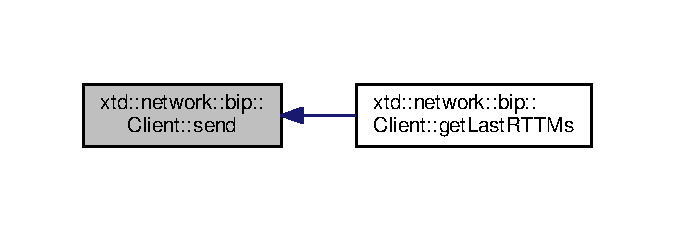
\includegraphics[width=324pt]{classxtd_1_1network_1_1bip_1_1Client_acda47c19d4fc71705f4db91226cec1b9_icgraph}
\end{center}
\end{figure}


\index{xtd\+::network\+::bip\+::\+Client@{xtd\+::network\+::bip\+::\+Client}!should\+Receive@{should\+Receive}}
\index{should\+Receive@{should\+Receive}!xtd\+::network\+::bip\+::\+Client@{xtd\+::network\+::bip\+::\+Client}}
\subsubsection[{\texorpdfstring{should\+Receive(const T\+Request \&p\+\_\+request, const bool p\+\_\+request\+Debug)}{shouldReceive(const TRequest &p_request, const bool p_requestDebug)}}]{\setlength{\rightskip}{0pt plus 5cm}template$<$class T\+Request , class T\+Response , typename T\+Domain  = utils\+::af\+\_\+inet$>$ virtual bool {\bf xtd\+::network\+::bip\+::\+Client}$<$ T\+Request, T\+Response, T\+Domain $>$\+::should\+Receive (
\begin{DoxyParamCaption}
\item[{const T\+Request \&}]{p\+\_\+request, }
\item[{const bool}]{p\+\_\+request\+Debug}
\end{DoxyParamCaption}
)\hspace{0.3cm}{\ttfamily [virtual]}}\hypertarget{classxtd_1_1network_1_1bip_1_1Client_a5721e7ec64739ab5a252d5ac59e4a86e}{}\label{classxtd_1_1network_1_1bip_1_1Client_a5721e7ec64739ab5a252d5ac59e4a86e}


Here is the caller graph for this function\+:
\nopagebreak
\begin{figure}[H]
\begin{center}
\leavevmode
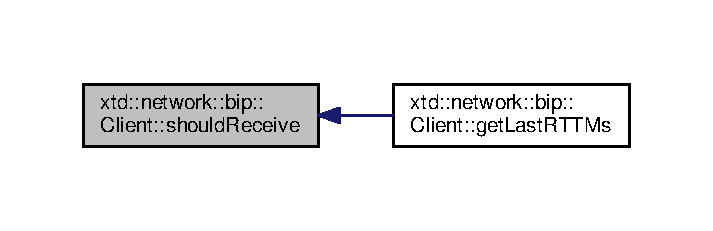
\includegraphics[width=342pt]{classxtd_1_1network_1_1bip_1_1Client_a5721e7ec64739ab5a252d5ac59e4a86e_icgraph}
\end{center}
\end{figure}




The documentation for this class was generated from the following file\+:\begin{DoxyCompactItemize}
\item 
/home/psyco/dev/xtdcpp/network/src/bip/\hyperlink{bip_2Client_8hh}{Client.\+hh}\end{DoxyCompactItemize}

\hypertarget{classxtd_1_1network_1_1bip_1_1ClientPool}{\section{xtd\-:\-:network\-:\-:bip\-:\-:Client\-Pool$<$ T\-Request, T\-Response, T\-Domain $>$ Class Template Reference}
\label{classxtd_1_1network_1_1bip_1_1ClientPool}\index{xtd\-::network\-::bip\-::\-Client\-Pool$<$ T\-Request, T\-Response, T\-Domain $>$@{xtd\-::network\-::bip\-::\-Client\-Pool$<$ T\-Request, T\-Response, T\-Domain $>$}}
}


{\ttfamily \#include $<$Client\-Pool.\-hh$>$}

\subsection*{Classes}
\begin{DoxyCompactItemize}
\item 
class \hyperlink{classxtd_1_1network_1_1bip_1_1ClientPool_1_1PersistentClient}{Persistent\-Client}
\end{DoxyCompactItemize}
\subsection*{Public Types}
\begin{DoxyCompactItemize}
\item 
typedef boost\-::shared\-\_\-ptr\\*
$<$ \hyperlink{classxtd_1_1network_1_1bip_1_1ClientPool_1_1PersistentClient}{Persistent\-Client} $>$ \hyperlink{classxtd_1_1network_1_1bip_1_1ClientPool_ac3b215a76aeb124011801824f993a52b}{t\-\_\-client\-\_\-sptr}
\item 
typedef std\-::deque$<$ \hyperlink{classxtd_1_1network_1_1bip_1_1ClientPool_ac3b215a76aeb124011801824f993a52b}{t\-\_\-client\-\_\-sptr} $>$ \hyperlink{classxtd_1_1network_1_1bip_1_1ClientPool_ab0b045804570a41e6e491a715d56a469}{t\-\_\-pool}
\end{DoxyCompactItemize}
\subsection*{Public Member Functions}
\begin{DoxyCompactItemize}
\item 
\hyperlink{classxtd_1_1network_1_1bip_1_1ClientPool_a19357fadc950be3b681e4c13b602b9ff}{Client\-Pool} (const string \&p\-\_\-hostname, const uint32\-\_\-t p\-\_\-port, const \hyperlink{classxtd_1_1network_1_1utils_1_1Config}{utils\-::\-Config} \&p\-\_\-conf, const uint32\-\_\-t p\-\_\-ttl\-Ms=20000)
\item 
const uint32\-\_\-t \& \hyperlink{classxtd_1_1network_1_1bip_1_1ClientPool_ac38bce359cae12634348f3baceb31668}{get\-Send\-Total} (void) const 
\item 
const uint32\-\_\-t \& \hyperlink{classxtd_1_1network_1_1bip_1_1ClientPool_ae744842f18c70979bf792d10fe799716}{get\-Send\-Success} (void) const 
\item 
const uint32\-\_\-t \& \hyperlink{classxtd_1_1network_1_1bip_1_1ClientPool_a48e713a842d7d5bf0c9142d4f65ab719}{get\-Send\-Error} (void) const 
\item 
const uint32\-\_\-t \& \hyperlink{classxtd_1_1network_1_1bip_1_1ClientPool_a65c430ef8ee5a65ec6289ea554df9ccf}{get\-Send\-Timeout} (void) const 
\item 
const uint32\-\_\-t \& \hyperlink{classxtd_1_1network_1_1bip_1_1ClientPool_aae35b25fd8d491a7b4e42dcb3b00dbc8}{get\-Rcv\-Total} (void) const 
\item 
const uint32\-\_\-t \& \hyperlink{classxtd_1_1network_1_1bip_1_1ClientPool_a118010103ded46a9d997765e74a9fddf}{get\-Rcv\-Success} (void) const 
\item 
const uint32\-\_\-t \& \hyperlink{classxtd_1_1network_1_1bip_1_1ClientPool_a44f712ba35d274fcb093c55f197539da}{get\-Rcv\-Error} (void) const 
\item 
const uint32\-\_\-t \& \hyperlink{classxtd_1_1network_1_1bip_1_1ClientPool_abdb1cb0ea47af82189a3df7e074ba123}{get\-Rcv\-Timeout} (void) const 
\item 
const uint32\-\_\-t \& \hyperlink{classxtd_1_1network_1_1bip_1_1ClientPool_a70de85e8b181bd82214bff2aa27600f1}{get\-Cur\-Nb\-Client} (void) const 
\item 
const uint32\-\_\-t \& \hyperlink{classxtd_1_1network_1_1bip_1_1ClientPool_a616b3398d55725cdf1cee89a9c7f1154}{get\-Recycle\-Hit} (void) const 
\item 
const uint32\-\_\-t \& \hyperlink{classxtd_1_1network_1_1bip_1_1ClientPool_a0432fecefc0e16d58581e71d9796a423}{get\-Recycle\-Miss} (void) const 
\item 
\hyperlink{classxtd_1_1network_1_1bip_1_1ClientPool_ac3b215a76aeb124011801824f993a52b}{t\-\_\-client\-\_\-sptr} \hyperlink{classxtd_1_1network_1_1bip_1_1ClientPool_a9d2d89926ce38e5fbb73ef297945c586}{acquire} (void)
\begin{DoxyCompactList}\small\item\em Réservation d'un client. \end{DoxyCompactList}\item 
status \hyperlink{classxtd_1_1network_1_1bip_1_1ClientPool_a1cba2c44a7995319a0aa2bbb7f823ff4}{send} (\hyperlink{classxtd_1_1network_1_1bip_1_1ClientPool_ac3b215a76aeb124011801824f993a52b}{t\-\_\-client\-\_\-sptr} \&p\-\_\-client, const T\-Request \&p\-\_\-request, bool p\-\_\-debug)
\begin{DoxyCompactList}\small\item\em Envoie d'une requete en utilisant l'identifiant de client reservé \end{DoxyCompactList}\item 
status \hyperlink{classxtd_1_1network_1_1bip_1_1ClientPool_a5884f162a9ca3dee26768eb1f683b6ec}{receive} (\hyperlink{classxtd_1_1network_1_1bip_1_1ClientPool_ac3b215a76aeb124011801824f993a52b}{t\-\_\-client\-\_\-sptr} \&p\-\_\-client, T\-Response \&p\-\_\-response, bool \&p\-\_\-debug)
\begin{DoxyCompactList}\small\item\em reception d'une reponse en utilisant l'identifiant de client reservé \end{DoxyCompactList}\item 
void \hyperlink{classxtd_1_1network_1_1bip_1_1ClientPool_a390ed6d8afa1812690fbe120bdea5059}{release} (\hyperlink{classxtd_1_1network_1_1bip_1_1ClientPool_ac3b215a76aeb124011801824f993a52b}{t\-\_\-client\-\_\-sptr} \&p\-\_\-client)
\begin{DoxyCompactList}\small\item\em libration d'un client reservé \end{DoxyCompactList}\end{DoxyCompactItemize}


\subsection{Detailed Description}
\subsubsection*{template$<$class T\-Request, class T\-Response, typename T\-Domain = utils\-::af\-\_\-inet$>$class xtd\-::network\-::bip\-::\-Client\-Pool$<$ T\-Request, T\-Response, T\-Domain $>$}



Definition at line 22 of file Client\-Pool.\-hh.



\subsection{Member Typedef Documentation}
\hypertarget{classxtd_1_1network_1_1bip_1_1ClientPool_ac3b215a76aeb124011801824f993a52b}{\index{xtd\-::network\-::bip\-::\-Client\-Pool@{xtd\-::network\-::bip\-::\-Client\-Pool}!t\-\_\-client\-\_\-sptr@{t\-\_\-client\-\_\-sptr}}
\index{t\-\_\-client\-\_\-sptr@{t\-\_\-client\-\_\-sptr}!xtd::network::bip::ClientPool@{xtd\-::network\-::bip\-::\-Client\-Pool}}
\subsubsection[{t\-\_\-client\-\_\-sptr}]{\setlength{\rightskip}{0pt plus 5cm}template$<$class T\-Request , class T\-Response , typename T\-Domain  = utils\-::af\-\_\-inet$>$ typedef boost\-::shared\-\_\-ptr$<${\bf Persistent\-Client}$>$ {\bf xtd\-::network\-::bip\-::\-Client\-Pool}$<$ T\-Request, T\-Response, T\-Domain $>$\-::{\bf t\-\_\-client\-\_\-sptr}}}\label{classxtd_1_1network_1_1bip_1_1ClientPool_ac3b215a76aeb124011801824f993a52b}


Definition at line 53 of file Client\-Pool.\-hh.

\hypertarget{classxtd_1_1network_1_1bip_1_1ClientPool_ab0b045804570a41e6e491a715d56a469}{\index{xtd\-::network\-::bip\-::\-Client\-Pool@{xtd\-::network\-::bip\-::\-Client\-Pool}!t\-\_\-pool@{t\-\_\-pool}}
\index{t\-\_\-pool@{t\-\_\-pool}!xtd::network::bip::ClientPool@{xtd\-::network\-::bip\-::\-Client\-Pool}}
\subsubsection[{t\-\_\-pool}]{\setlength{\rightskip}{0pt plus 5cm}template$<$class T\-Request , class T\-Response , typename T\-Domain  = utils\-::af\-\_\-inet$>$ typedef std\-::deque$<${\bf t\-\_\-client\-\_\-sptr}$>$ {\bf xtd\-::network\-::bip\-::\-Client\-Pool}$<$ T\-Request, T\-Response, T\-Domain $>$\-::{\bf t\-\_\-pool}}}\label{classxtd_1_1network_1_1bip_1_1ClientPool_ab0b045804570a41e6e491a715d56a469}


Definition at line 54 of file Client\-Pool.\-hh.



\subsection{Constructor \& Destructor Documentation}
\hypertarget{classxtd_1_1network_1_1bip_1_1ClientPool_a19357fadc950be3b681e4c13b602b9ff}{\index{xtd\-::network\-::bip\-::\-Client\-Pool@{xtd\-::network\-::bip\-::\-Client\-Pool}!Client\-Pool@{Client\-Pool}}
\index{Client\-Pool@{Client\-Pool}!xtd::network::bip::ClientPool@{xtd\-::network\-::bip\-::\-Client\-Pool}}
\subsubsection[{Client\-Pool}]{\setlength{\rightskip}{0pt plus 5cm}template$<$class T\-Request , class T\-Response , typename T\-Domain  = utils\-::af\-\_\-inet$>$ {\bf xtd\-::network\-::bip\-::\-Client\-Pool}$<$ T\-Request, T\-Response, T\-Domain $>$\-::{\bf Client\-Pool} (
\begin{DoxyParamCaption}
\item[{const string \&}]{p\-\_\-hostname, }
\item[{const uint32\-\_\-t}]{p\-\_\-port, }
\item[{const {\bf utils\-::\-Config} \&}]{p\-\_\-conf, }
\item[{const uint32\-\_\-t}]{p\-\_\-ttl\-Ms = {\ttfamily 20000}}
\end{DoxyParamCaption}
)}}\label{classxtd_1_1network_1_1bip_1_1ClientPool_a19357fadc950be3b681e4c13b602b9ff}
Constructor 

\subsection{Member Function Documentation}
\hypertarget{classxtd_1_1network_1_1bip_1_1ClientPool_a9d2d89926ce38e5fbb73ef297945c586}{\index{xtd\-::network\-::bip\-::\-Client\-Pool@{xtd\-::network\-::bip\-::\-Client\-Pool}!acquire@{acquire}}
\index{acquire@{acquire}!xtd::network::bip::ClientPool@{xtd\-::network\-::bip\-::\-Client\-Pool}}
\subsubsection[{acquire}]{\setlength{\rightskip}{0pt plus 5cm}template$<$class T\-Request , class T\-Response , typename T\-Domain  = utils\-::af\-\_\-inet$>$ {\bf t\-\_\-client\-\_\-sptr} {\bf xtd\-::network\-::bip\-::\-Client\-Pool}$<$ T\-Request, T\-Response, T\-Domain $>$\-::acquire (
\begin{DoxyParamCaption}
\item[{void}]{}
\end{DoxyParamCaption}
)}}\label{classxtd_1_1network_1_1bip_1_1ClientPool_a9d2d89926ce38e5fbb73ef297945c586}


Réservation d'un client. 

\hypertarget{classxtd_1_1network_1_1bip_1_1ClientPool_a70de85e8b181bd82214bff2aa27600f1}{\index{xtd\-::network\-::bip\-::\-Client\-Pool@{xtd\-::network\-::bip\-::\-Client\-Pool}!get\-Cur\-Nb\-Client@{get\-Cur\-Nb\-Client}}
\index{get\-Cur\-Nb\-Client@{get\-Cur\-Nb\-Client}!xtd::network::bip::ClientPool@{xtd\-::network\-::bip\-::\-Client\-Pool}}
\subsubsection[{get\-Cur\-Nb\-Client}]{\setlength{\rightskip}{0pt plus 5cm}template$<$class T\-Request , class T\-Response , typename T\-Domain  = utils\-::af\-\_\-inet$>$ const uint32\-\_\-t\& {\bf xtd\-::network\-::bip\-::\-Client\-Pool}$<$ T\-Request, T\-Response, T\-Domain $>$\-::get\-Cur\-Nb\-Client (
\begin{DoxyParamCaption}
\item[{void}]{}
\end{DoxyParamCaption}
) const\hspace{0.3cm}{\ttfamily [inline]}}}\label{classxtd_1_1network_1_1bip_1_1ClientPool_a70de85e8b181bd82214bff2aa27600f1}


Definition at line 74 of file Client\-Pool.\-hh.


\begin{DoxyCode}
74 \{ \textcolor{keywordflow}{return} m\_curNbClient; \}
\end{DoxyCode}
\hypertarget{classxtd_1_1network_1_1bip_1_1ClientPool_a44f712ba35d274fcb093c55f197539da}{\index{xtd\-::network\-::bip\-::\-Client\-Pool@{xtd\-::network\-::bip\-::\-Client\-Pool}!get\-Rcv\-Error@{get\-Rcv\-Error}}
\index{get\-Rcv\-Error@{get\-Rcv\-Error}!xtd::network::bip::ClientPool@{xtd\-::network\-::bip\-::\-Client\-Pool}}
\subsubsection[{get\-Rcv\-Error}]{\setlength{\rightskip}{0pt plus 5cm}template$<$class T\-Request , class T\-Response , typename T\-Domain  = utils\-::af\-\_\-inet$>$ const uint32\-\_\-t\& {\bf xtd\-::network\-::bip\-::\-Client\-Pool}$<$ T\-Request, T\-Response, T\-Domain $>$\-::get\-Rcv\-Error (
\begin{DoxyParamCaption}
\item[{void}]{}
\end{DoxyParamCaption}
) const\hspace{0.3cm}{\ttfamily [inline]}}}\label{classxtd_1_1network_1_1bip_1_1ClientPool_a44f712ba35d274fcb093c55f197539da}


Definition at line 72 of file Client\-Pool.\-hh.


\begin{DoxyCode}
72 \{ \textcolor{keywordflow}{return} m\_rcvError;    \}
\end{DoxyCode}
\hypertarget{classxtd_1_1network_1_1bip_1_1ClientPool_a118010103ded46a9d997765e74a9fddf}{\index{xtd\-::network\-::bip\-::\-Client\-Pool@{xtd\-::network\-::bip\-::\-Client\-Pool}!get\-Rcv\-Success@{get\-Rcv\-Success}}
\index{get\-Rcv\-Success@{get\-Rcv\-Success}!xtd::network::bip::ClientPool@{xtd\-::network\-::bip\-::\-Client\-Pool}}
\subsubsection[{get\-Rcv\-Success}]{\setlength{\rightskip}{0pt plus 5cm}template$<$class T\-Request , class T\-Response , typename T\-Domain  = utils\-::af\-\_\-inet$>$ const uint32\-\_\-t\& {\bf xtd\-::network\-::bip\-::\-Client\-Pool}$<$ T\-Request, T\-Response, T\-Domain $>$\-::get\-Rcv\-Success (
\begin{DoxyParamCaption}
\item[{void}]{}
\end{DoxyParamCaption}
) const\hspace{0.3cm}{\ttfamily [inline]}}}\label{classxtd_1_1network_1_1bip_1_1ClientPool_a118010103ded46a9d997765e74a9fddf}


Definition at line 71 of file Client\-Pool.\-hh.


\begin{DoxyCode}
71 \{ \textcolor{keywordflow}{return} m\_rcvSuccess;  \}
\end{DoxyCode}
\hypertarget{classxtd_1_1network_1_1bip_1_1ClientPool_abdb1cb0ea47af82189a3df7e074ba123}{\index{xtd\-::network\-::bip\-::\-Client\-Pool@{xtd\-::network\-::bip\-::\-Client\-Pool}!get\-Rcv\-Timeout@{get\-Rcv\-Timeout}}
\index{get\-Rcv\-Timeout@{get\-Rcv\-Timeout}!xtd::network::bip::ClientPool@{xtd\-::network\-::bip\-::\-Client\-Pool}}
\subsubsection[{get\-Rcv\-Timeout}]{\setlength{\rightskip}{0pt plus 5cm}template$<$class T\-Request , class T\-Response , typename T\-Domain  = utils\-::af\-\_\-inet$>$ const uint32\-\_\-t\& {\bf xtd\-::network\-::bip\-::\-Client\-Pool}$<$ T\-Request, T\-Response, T\-Domain $>$\-::get\-Rcv\-Timeout (
\begin{DoxyParamCaption}
\item[{void}]{}
\end{DoxyParamCaption}
) const\hspace{0.3cm}{\ttfamily [inline]}}}\label{classxtd_1_1network_1_1bip_1_1ClientPool_abdb1cb0ea47af82189a3df7e074ba123}


Definition at line 73 of file Client\-Pool.\-hh.


\begin{DoxyCode}
73 \{ \textcolor{keywordflow}{return} m\_rcvTimeout;  \}
\end{DoxyCode}
\hypertarget{classxtd_1_1network_1_1bip_1_1ClientPool_aae35b25fd8d491a7b4e42dcb3b00dbc8}{\index{xtd\-::network\-::bip\-::\-Client\-Pool@{xtd\-::network\-::bip\-::\-Client\-Pool}!get\-Rcv\-Total@{get\-Rcv\-Total}}
\index{get\-Rcv\-Total@{get\-Rcv\-Total}!xtd::network::bip::ClientPool@{xtd\-::network\-::bip\-::\-Client\-Pool}}
\subsubsection[{get\-Rcv\-Total}]{\setlength{\rightskip}{0pt plus 5cm}template$<$class T\-Request , class T\-Response , typename T\-Domain  = utils\-::af\-\_\-inet$>$ const uint32\-\_\-t\& {\bf xtd\-::network\-::bip\-::\-Client\-Pool}$<$ T\-Request, T\-Response, T\-Domain $>$\-::get\-Rcv\-Total (
\begin{DoxyParamCaption}
\item[{void}]{}
\end{DoxyParamCaption}
) const\hspace{0.3cm}{\ttfamily [inline]}}}\label{classxtd_1_1network_1_1bip_1_1ClientPool_aae35b25fd8d491a7b4e42dcb3b00dbc8}


Definition at line 70 of file Client\-Pool.\-hh.


\begin{DoxyCode}
70 \{ \textcolor{keywordflow}{return} m\_rcvTotal;    \}
\end{DoxyCode}
\hypertarget{classxtd_1_1network_1_1bip_1_1ClientPool_a616b3398d55725cdf1cee89a9c7f1154}{\index{xtd\-::network\-::bip\-::\-Client\-Pool@{xtd\-::network\-::bip\-::\-Client\-Pool}!get\-Recycle\-Hit@{get\-Recycle\-Hit}}
\index{get\-Recycle\-Hit@{get\-Recycle\-Hit}!xtd::network::bip::ClientPool@{xtd\-::network\-::bip\-::\-Client\-Pool}}
\subsubsection[{get\-Recycle\-Hit}]{\setlength{\rightskip}{0pt plus 5cm}template$<$class T\-Request , class T\-Response , typename T\-Domain  = utils\-::af\-\_\-inet$>$ const uint32\-\_\-t\& {\bf xtd\-::network\-::bip\-::\-Client\-Pool}$<$ T\-Request, T\-Response, T\-Domain $>$\-::get\-Recycle\-Hit (
\begin{DoxyParamCaption}
\item[{void}]{}
\end{DoxyParamCaption}
) const\hspace{0.3cm}{\ttfamily [inline]}}}\label{classxtd_1_1network_1_1bip_1_1ClientPool_a616b3398d55725cdf1cee89a9c7f1154}


Definition at line 75 of file Client\-Pool.\-hh.


\begin{DoxyCode}
75 \{ \textcolor{keywordflow}{return} m\_recycleHit;  \}
\end{DoxyCode}
\hypertarget{classxtd_1_1network_1_1bip_1_1ClientPool_a0432fecefc0e16d58581e71d9796a423}{\index{xtd\-::network\-::bip\-::\-Client\-Pool@{xtd\-::network\-::bip\-::\-Client\-Pool}!get\-Recycle\-Miss@{get\-Recycle\-Miss}}
\index{get\-Recycle\-Miss@{get\-Recycle\-Miss}!xtd::network::bip::ClientPool@{xtd\-::network\-::bip\-::\-Client\-Pool}}
\subsubsection[{get\-Recycle\-Miss}]{\setlength{\rightskip}{0pt plus 5cm}template$<$class T\-Request , class T\-Response , typename T\-Domain  = utils\-::af\-\_\-inet$>$ const uint32\-\_\-t\& {\bf xtd\-::network\-::bip\-::\-Client\-Pool}$<$ T\-Request, T\-Response, T\-Domain $>$\-::get\-Recycle\-Miss (
\begin{DoxyParamCaption}
\item[{void}]{}
\end{DoxyParamCaption}
) const\hspace{0.3cm}{\ttfamily [inline]}}}\label{classxtd_1_1network_1_1bip_1_1ClientPool_a0432fecefc0e16d58581e71d9796a423}


Definition at line 76 of file Client\-Pool.\-hh.


\begin{DoxyCode}
76 \{ \textcolor{keywordflow}{return} m\_recycleMiss; \}
\end{DoxyCode}
\hypertarget{classxtd_1_1network_1_1bip_1_1ClientPool_a48e713a842d7d5bf0c9142d4f65ab719}{\index{xtd\-::network\-::bip\-::\-Client\-Pool@{xtd\-::network\-::bip\-::\-Client\-Pool}!get\-Send\-Error@{get\-Send\-Error}}
\index{get\-Send\-Error@{get\-Send\-Error}!xtd::network::bip::ClientPool@{xtd\-::network\-::bip\-::\-Client\-Pool}}
\subsubsection[{get\-Send\-Error}]{\setlength{\rightskip}{0pt plus 5cm}template$<$class T\-Request , class T\-Response , typename T\-Domain  = utils\-::af\-\_\-inet$>$ const uint32\-\_\-t\& {\bf xtd\-::network\-::bip\-::\-Client\-Pool}$<$ T\-Request, T\-Response, T\-Domain $>$\-::get\-Send\-Error (
\begin{DoxyParamCaption}
\item[{void}]{}
\end{DoxyParamCaption}
) const\hspace{0.3cm}{\ttfamily [inline]}}}\label{classxtd_1_1network_1_1bip_1_1ClientPool_a48e713a842d7d5bf0c9142d4f65ab719}


Definition at line 68 of file Client\-Pool.\-hh.


\begin{DoxyCode}
68 \{ \textcolor{keywordflow}{return} m\_sendError;   \}
\end{DoxyCode}
\hypertarget{classxtd_1_1network_1_1bip_1_1ClientPool_ae744842f18c70979bf792d10fe799716}{\index{xtd\-::network\-::bip\-::\-Client\-Pool@{xtd\-::network\-::bip\-::\-Client\-Pool}!get\-Send\-Success@{get\-Send\-Success}}
\index{get\-Send\-Success@{get\-Send\-Success}!xtd::network::bip::ClientPool@{xtd\-::network\-::bip\-::\-Client\-Pool}}
\subsubsection[{get\-Send\-Success}]{\setlength{\rightskip}{0pt plus 5cm}template$<$class T\-Request , class T\-Response , typename T\-Domain  = utils\-::af\-\_\-inet$>$ const uint32\-\_\-t\& {\bf xtd\-::network\-::bip\-::\-Client\-Pool}$<$ T\-Request, T\-Response, T\-Domain $>$\-::get\-Send\-Success (
\begin{DoxyParamCaption}
\item[{void}]{}
\end{DoxyParamCaption}
) const\hspace{0.3cm}{\ttfamily [inline]}}}\label{classxtd_1_1network_1_1bip_1_1ClientPool_ae744842f18c70979bf792d10fe799716}


Definition at line 67 of file Client\-Pool.\-hh.


\begin{DoxyCode}
67 \{ \textcolor{keywordflow}{return} m\_sendSuccess; \}
\end{DoxyCode}
\hypertarget{classxtd_1_1network_1_1bip_1_1ClientPool_a65c430ef8ee5a65ec6289ea554df9ccf}{\index{xtd\-::network\-::bip\-::\-Client\-Pool@{xtd\-::network\-::bip\-::\-Client\-Pool}!get\-Send\-Timeout@{get\-Send\-Timeout}}
\index{get\-Send\-Timeout@{get\-Send\-Timeout}!xtd::network::bip::ClientPool@{xtd\-::network\-::bip\-::\-Client\-Pool}}
\subsubsection[{get\-Send\-Timeout}]{\setlength{\rightskip}{0pt plus 5cm}template$<$class T\-Request , class T\-Response , typename T\-Domain  = utils\-::af\-\_\-inet$>$ const uint32\-\_\-t\& {\bf xtd\-::network\-::bip\-::\-Client\-Pool}$<$ T\-Request, T\-Response, T\-Domain $>$\-::get\-Send\-Timeout (
\begin{DoxyParamCaption}
\item[{void}]{}
\end{DoxyParamCaption}
) const\hspace{0.3cm}{\ttfamily [inline]}}}\label{classxtd_1_1network_1_1bip_1_1ClientPool_a65c430ef8ee5a65ec6289ea554df9ccf}


Definition at line 69 of file Client\-Pool.\-hh.


\begin{DoxyCode}
69 \{ \textcolor{keywordflow}{return} m\_sendTimeout; \}
\end{DoxyCode}
\hypertarget{classxtd_1_1network_1_1bip_1_1ClientPool_ac38bce359cae12634348f3baceb31668}{\index{xtd\-::network\-::bip\-::\-Client\-Pool@{xtd\-::network\-::bip\-::\-Client\-Pool}!get\-Send\-Total@{get\-Send\-Total}}
\index{get\-Send\-Total@{get\-Send\-Total}!xtd::network::bip::ClientPool@{xtd\-::network\-::bip\-::\-Client\-Pool}}
\subsubsection[{get\-Send\-Total}]{\setlength{\rightskip}{0pt plus 5cm}template$<$class T\-Request , class T\-Response , typename T\-Domain  = utils\-::af\-\_\-inet$>$ const uint32\-\_\-t\& {\bf xtd\-::network\-::bip\-::\-Client\-Pool}$<$ T\-Request, T\-Response, T\-Domain $>$\-::get\-Send\-Total (
\begin{DoxyParamCaption}
\item[{void}]{}
\end{DoxyParamCaption}
) const\hspace{0.3cm}{\ttfamily [inline]}}}\label{classxtd_1_1network_1_1bip_1_1ClientPool_ac38bce359cae12634348f3baceb31668}


Definition at line 66 of file Client\-Pool.\-hh.


\begin{DoxyCode}
66 \{ \textcolor{keywordflow}{return} m\_sendTotal;   \}
\end{DoxyCode}
\hypertarget{classxtd_1_1network_1_1bip_1_1ClientPool_a5884f162a9ca3dee26768eb1f683b6ec}{\index{xtd\-::network\-::bip\-::\-Client\-Pool@{xtd\-::network\-::bip\-::\-Client\-Pool}!receive@{receive}}
\index{receive@{receive}!xtd::network::bip::ClientPool@{xtd\-::network\-::bip\-::\-Client\-Pool}}
\subsubsection[{receive}]{\setlength{\rightskip}{0pt plus 5cm}template$<$class T\-Request , class T\-Response , typename T\-Domain  = utils\-::af\-\_\-inet$>$ status {\bf xtd\-::network\-::bip\-::\-Client\-Pool}$<$ T\-Request, T\-Response, T\-Domain $>$\-::receive (
\begin{DoxyParamCaption}
\item[{{\bf t\-\_\-client\-\_\-sptr} \&}]{p\-\_\-client, }
\item[{T\-Response \&}]{p\-\_\-response, }
\item[{bool \&}]{p\-\_\-debug}
\end{DoxyParamCaption}
)}}\label{classxtd_1_1network_1_1bip_1_1ClientPool_a5884f162a9ca3dee26768eb1f683b6ec}


reception d'une reponse en utilisant l'identifiant de client reservé 

\hypertarget{classxtd_1_1network_1_1bip_1_1ClientPool_a390ed6d8afa1812690fbe120bdea5059}{\index{xtd\-::network\-::bip\-::\-Client\-Pool@{xtd\-::network\-::bip\-::\-Client\-Pool}!release@{release}}
\index{release@{release}!xtd::network::bip::ClientPool@{xtd\-::network\-::bip\-::\-Client\-Pool}}
\subsubsection[{release}]{\setlength{\rightskip}{0pt plus 5cm}template$<$class T\-Request , class T\-Response , typename T\-Domain  = utils\-::af\-\_\-inet$>$ void {\bf xtd\-::network\-::bip\-::\-Client\-Pool}$<$ T\-Request, T\-Response, T\-Domain $>$\-::release (
\begin{DoxyParamCaption}
\item[{{\bf t\-\_\-client\-\_\-sptr} \&}]{p\-\_\-client}
\end{DoxyParamCaption}
)}}\label{classxtd_1_1network_1_1bip_1_1ClientPool_a390ed6d8afa1812690fbe120bdea5059}


libration d'un client reservé 

\hypertarget{classxtd_1_1network_1_1bip_1_1ClientPool_a1cba2c44a7995319a0aa2bbb7f823ff4}{\index{xtd\-::network\-::bip\-::\-Client\-Pool@{xtd\-::network\-::bip\-::\-Client\-Pool}!send@{send}}
\index{send@{send}!xtd::network::bip::ClientPool@{xtd\-::network\-::bip\-::\-Client\-Pool}}
\subsubsection[{send}]{\setlength{\rightskip}{0pt plus 5cm}template$<$class T\-Request , class T\-Response , typename T\-Domain  = utils\-::af\-\_\-inet$>$ status {\bf xtd\-::network\-::bip\-::\-Client\-Pool}$<$ T\-Request, T\-Response, T\-Domain $>$\-::send (
\begin{DoxyParamCaption}
\item[{{\bf t\-\_\-client\-\_\-sptr} \&}]{p\-\_\-client, }
\item[{const T\-Request \&}]{p\-\_\-request, }
\item[{bool}]{p\-\_\-debug}
\end{DoxyParamCaption}
)}}\label{classxtd_1_1network_1_1bip_1_1ClientPool_a1cba2c44a7995319a0aa2bbb7f823ff4}


Envoie d'une requete en utilisant l'identifiant de client reservé 



The documentation for this class was generated from the following file\-:\begin{DoxyCompactItemize}
\item 
/home/travis/build/psycofdj/xtdcpp/network/src/bip/\hyperlink{ClientPool_8hh}{Client\-Pool.\-hh}\end{DoxyCompactItemize}

\hypertarget{classxtd_1_1network_1_1utils_1_1Config}{}\section{xtd\+:\+:network\+:\+:utils\+:\+:Config Class Reference}
\label{classxtd_1_1network_1_1utils_1_1Config}\index{xtd\+::network\+::utils\+::\+Config@{xtd\+::network\+::utils\+::\+Config}}


{\ttfamily \#include $<$Config.\+hh$>$}

\subsection*{Public Member Functions}
\begin{DoxyCompactItemize}
\item 
\hyperlink{classxtd_1_1network_1_1utils_1_1Config_a38494ac8cb1f19047196843e3b911f8a}{Config} (void)
\begin{DoxyCompactList}\small\item\em default constructor set nothing \end{DoxyCompactList}\item 
\hyperlink{classxtd_1_1network_1_1utils_1_1Config_abbf53027f45806e78cec4f50e4ea7def}{Config} (uint32\+\_\+t p\+\_\+flags, uint32\+\_\+t p\+\_\+linger\+Interval=0)
\begin{DoxyCompactList}\small\item\em Constructor make the socket setting. \end{DoxyCompactList}\item 
bool \hyperlink{classxtd_1_1network_1_1utils_1_1Config_ab43d43856cea3b9bf159b38d2d13d82b}{get\+Linger} (void) const 
\item 
uint32\+\_\+t \hyperlink{classxtd_1_1network_1_1utils_1_1Config_aacb13cdd90746d5684feb00d7cdbefcc}{get\+Linger\+Time} (void) const 
\item 
bool \hyperlink{classxtd_1_1network_1_1utils_1_1Config_a499712a4fd63e48be43ff24eb94e72ff}{get\+No\+Delay} (void) const 
\item 
bool \hyperlink{classxtd_1_1network_1_1utils_1_1Config_a3914a56737d69dd8879e03ed9b3dc855}{get\+Reuse\+Addr} (void) const 
\item 
bool \hyperlink{classxtd_1_1network_1_1utils_1_1Config_a89faeb4f4a949ae6fe18b907814987ee}{get\+Compress} (void) const 
\item 
\hyperlink{namespacextd_1_1network_1_1utils_a3ac1216ad2037b366cc1f9051a978161}{codec} \hyperlink{classxtd_1_1network_1_1utils_1_1Config_a82a7b809f4d41f4124badef452b9698d}{get\+Compression\+Codec} (void) const 
\item 
uint32\+\_\+t \hyperlink{classxtd_1_1network_1_1utils_1_1Config_a2dfd5c85238ef930891d3696e6f6246c}{get\+Connect\+Timeout\+Ms} (void) const 
\item 
uint32\+\_\+t \hyperlink{classxtd_1_1network_1_1utils_1_1Config_a300d76106dcc338d662894dd04373d91}{get\+Send\+Timeout\+Ms} (void) const 
\item 
uint32\+\_\+t \hyperlink{classxtd_1_1network_1_1utils_1_1Config_a4484d8887f26682beb5aaa45f801dc57}{get\+Receive\+Timeout\+Ms} (void) const 
\item 
uint32\+\_\+t \hyperlink{classxtd_1_1network_1_1utils_1_1Config_a1ef6d7fcee95df86143dfbdd007f64f9}{get\+Dns\+Cache\+T\+TL} (void) const 
\item 
void \hyperlink{classxtd_1_1network_1_1utils_1_1Config_a1a0e52354981c89c5aaf2b31d4490de2}{set\+Linger} (bool p\+\_\+linger, uint32\+\_\+t p\+\_\+linger\+Time)
\item 
void \hyperlink{classxtd_1_1network_1_1utils_1_1Config_a1dbcee3c0f2631269ea3e716a62ce333}{set\+No\+Delay} (bool p\+\_\+no\+Delay)
\item 
void \hyperlink{classxtd_1_1network_1_1utils_1_1Config_a5e78cf9920484c88da5f42bae16b7a1f}{set\+Reuse\+Addr} (bool p\+\_\+reuse\+Addr)
\item 
void \hyperlink{classxtd_1_1network_1_1utils_1_1Config_aab76e2174465ead19cc97fa3f5a7f009}{set\+Compress} (bool p\+\_\+compress)
\item 
void \hyperlink{classxtd_1_1network_1_1utils_1_1Config_a604e4ade1c49d83d204024f28a3d461d}{set\+Compression\+Codec} (\hyperlink{namespacextd_1_1network_1_1utils_a3ac1216ad2037b366cc1f9051a978161}{codec} p\+\_\+compression\+Codec)
\item 
void \hyperlink{classxtd_1_1network_1_1utils_1_1Config_a5ecd1cd77dd3bd937aa021d3bf0ad860}{set\+Connect\+Timeout\+Ms} (uint32\+\_\+t p\+\_\+ms)
\item 
void \hyperlink{classxtd_1_1network_1_1utils_1_1Config_a583358bf6945cbddd657f6db8c31618e}{set\+Send\+Timeout\+Ms} (uint32\+\_\+t p\+\_\+ms)
\item 
void \hyperlink{classxtd_1_1network_1_1utils_1_1Config_ad633fb35c7202550d444e4bf5ae213df}{set\+Receive\+Timeout\+Ms} (uint32\+\_\+t p\+\_\+ms)
\item 
void \hyperlink{classxtd_1_1network_1_1utils_1_1Config_a9a2d3e9de6f26708a4bddc4ba7c31428}{set\+Dns\+Cache\+T\+TL} (uint32\+\_\+t p\+\_\+ms)
\end{DoxyCompactItemize}


\subsection{Detailed Description}


Definition at line 17 of file Config.\+hh.



\subsection{Constructor \& Destructor Documentation}
\index{xtd\+::network\+::utils\+::\+Config@{xtd\+::network\+::utils\+::\+Config}!Config@{Config}}
\index{Config@{Config}!xtd\+::network\+::utils\+::\+Config@{xtd\+::network\+::utils\+::\+Config}}
\subsubsection[{\texorpdfstring{Config(void)}{Config(void)}}]{\setlength{\rightskip}{0pt plus 5cm}xtd\+::network\+::utils\+::\+Config\+::\+Config (
\begin{DoxyParamCaption}
\item[{void}]{}
\end{DoxyParamCaption}
)}\hypertarget{classxtd_1_1network_1_1utils_1_1Config_a38494ac8cb1f19047196843e3b911f8a}{}\label{classxtd_1_1network_1_1utils_1_1Config_a38494ac8cb1f19047196843e3b911f8a}


default constructor set nothing 



Definition at line 8 of file Config.\+cc.


\begin{DoxyCode}
8                    :
9   m\_noDelay(\textcolor{keyword}{false}),
10   m\_reuseAddr(\textcolor{keyword}{false}),
11   m\_linger(\textcolor{keyword}{false}),
12   m\_lingerTime(0),
13   m\_compress(\textcolor{keyword}{false}),
14   m\_compressionCodec(\hyperlink{namespacextd_1_1network_1_1utils_a3ac1216ad2037b366cc1f9051a978161a7a990d405d2c6fb93aa8fbb0ec1a3b23}{codec::zlib}),
15   m\_dnsCacheTTL(1800),
16   m\_connectTimeoutMs(1800),
17   m\_sendTimeoutMs(1800),
18   m\_receiveTimeoutMs(1800)
19 \{
20 \}
\end{DoxyCode}
\index{xtd\+::network\+::utils\+::\+Config@{xtd\+::network\+::utils\+::\+Config}!Config@{Config}}
\index{Config@{Config}!xtd\+::network\+::utils\+::\+Config@{xtd\+::network\+::utils\+::\+Config}}
\subsubsection[{\texorpdfstring{Config(uint32\+\_\+t p\+\_\+flags, uint32\+\_\+t p\+\_\+linger\+Interval=0)}{Config(uint32_t p_flags, uint32_t p_lingerInterval=0)}}]{\setlength{\rightskip}{0pt plus 5cm}xtd\+::network\+::utils\+::\+Config\+::\+Config (
\begin{DoxyParamCaption}
\item[{uint32\+\_\+t}]{p\+\_\+flags, }
\item[{uint32\+\_\+t}]{p\+\_\+linger\+Interval = {\ttfamily 0}}
\end{DoxyParamCaption}
)}\hypertarget{classxtd_1_1network_1_1utils_1_1Config_abbf53027f45806e78cec4f50e4ea7def}{}\label{classxtd_1_1network_1_1utils_1_1Config_abbf53027f45806e78cec4f50e4ea7def}


Constructor make the socket setting. 


\begin{DoxyParams}{Parameters}
{\em p\+\_\+flags} & configuration flags \\
\hline
{\em p\+\_\+linger\+Interval} & linger interval \\
\hline
\end{DoxyParams}


Definition at line 22 of file Config.\+cc.


\begin{DoxyCode}
22                                                          :
23   m\_noDelay(\textcolor{keyword}{false}),
24   m\_reuseAddr(\textcolor{keyword}{false}),
25   m\_linger(\textcolor{keyword}{false}),
26   m\_lingerTime(0),
27   m\_compress(\textcolor{keyword}{false}),
28   m\_compressionCodec(\hyperlink{namespacextd_1_1network_1_1utils_a3ac1216ad2037b366cc1f9051a978161a7a990d405d2c6fb93aa8fbb0ec1a3b23}{codec::zlib}),
29   m\_dnsCacheTTL(1800),
30   m\_connectTimeoutMs(1800),
31   m\_sendTimeoutMs(1800),
32   m\_receiveTimeoutMs(1800)
33 \{
34   \hyperlink{classxtd_1_1network_1_1utils_1_1Config_a1dbcee3c0f2631269ea3e716a62ce333}{setNoDelay}   (p\_flags & valueof(\hyperlink{namespacextd_1_1network_1_1utils_a0acc888a3cdabdadb91fe832ea196a4faf0f888198330ff09558650aace4343e3}{option::nodelay}));
35   \hyperlink{classxtd_1_1network_1_1utils_1_1Config_a5e78cf9920484c88da5f42bae16b7a1f}{setReuseAddr} (p\_flags & valueof(\hyperlink{namespacextd_1_1network_1_1utils_a0acc888a3cdabdadb91fe832ea196a4fa087d20314d2967622b76fbf7ce91ebf2}{option::reuseaddr}));
36   \hyperlink{classxtd_1_1network_1_1utils_1_1Config_a1a0e52354981c89c5aaf2b31d4490de2}{setLinger}    (p\_flags & valueof(\hyperlink{namespacextd_1_1network_1_1utils_a0acc888a3cdabdadb91fe832ea196a4fafa1711bb276806d1f1808dbb0e31018a}{option::linger}), p\_lingerInterval);
37   \hyperlink{classxtd_1_1network_1_1utils_1_1Config_aab76e2174465ead19cc97fa3f5a7f009}{setCompress}  (p\_flags & valueof(\hyperlink{namespacextd_1_1network_1_1utils_a0acc888a3cdabdadb91fe832ea196a4fa390626c545194d0f20a704589b190994}{option::compress}));
38 \}
\end{DoxyCode}


Here is the call graph for this function\+:
\nopagebreak
\begin{figure}[H]
\begin{center}
\leavevmode
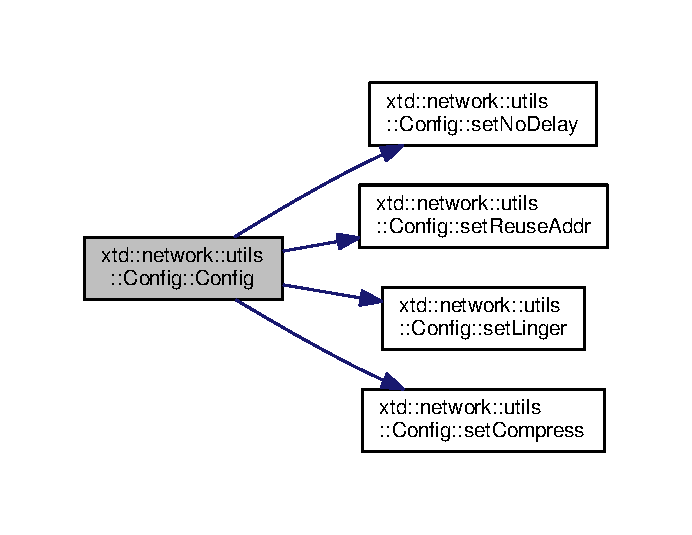
\includegraphics[width=330pt]{classxtd_1_1network_1_1utils_1_1Config_abbf53027f45806e78cec4f50e4ea7def_cgraph}
\end{center}
\end{figure}




\subsection{Member Function Documentation}
\index{xtd\+::network\+::utils\+::\+Config@{xtd\+::network\+::utils\+::\+Config}!get\+Compress@{get\+Compress}}
\index{get\+Compress@{get\+Compress}!xtd\+::network\+::utils\+::\+Config@{xtd\+::network\+::utils\+::\+Config}}
\subsubsection[{\texorpdfstring{get\+Compress(void) const }{getCompress(void) const }}]{\setlength{\rightskip}{0pt plus 5cm}bool xtd\+::network\+::utils\+::\+Config\+::get\+Compress (
\begin{DoxyParamCaption}
\item[{void}]{}
\end{DoxyParamCaption}
) const\hspace{0.3cm}{\ttfamily [inline]}}\hypertarget{classxtd_1_1network_1_1utils_1_1Config_a89faeb4f4a949ae6fe18b907814987ee}{}\label{classxtd_1_1network_1_1utils_1_1Config_a89faeb4f4a949ae6fe18b907814987ee}
\index{xtd\+::network\+::utils\+::\+Config@{xtd\+::network\+::utils\+::\+Config}!get\+Compression\+Codec@{get\+Compression\+Codec}}
\index{get\+Compression\+Codec@{get\+Compression\+Codec}!xtd\+::network\+::utils\+::\+Config@{xtd\+::network\+::utils\+::\+Config}}
\subsubsection[{\texorpdfstring{get\+Compression\+Codec(void) const }{getCompressionCodec(void) const }}]{\setlength{\rightskip}{0pt plus 5cm}{\bf codec} xtd\+::network\+::utils\+::\+Config\+::get\+Compression\+Codec (
\begin{DoxyParamCaption}
\item[{void}]{}
\end{DoxyParamCaption}
) const\hspace{0.3cm}{\ttfamily [inline]}}\hypertarget{classxtd_1_1network_1_1utils_1_1Config_a82a7b809f4d41f4124badef452b9698d}{}\label{classxtd_1_1network_1_1utils_1_1Config_a82a7b809f4d41f4124badef452b9698d}
\index{xtd\+::network\+::utils\+::\+Config@{xtd\+::network\+::utils\+::\+Config}!get\+Connect\+Timeout\+Ms@{get\+Connect\+Timeout\+Ms}}
\index{get\+Connect\+Timeout\+Ms@{get\+Connect\+Timeout\+Ms}!xtd\+::network\+::utils\+::\+Config@{xtd\+::network\+::utils\+::\+Config}}
\subsubsection[{\texorpdfstring{get\+Connect\+Timeout\+Ms(void) const }{getConnectTimeoutMs(void) const }}]{\setlength{\rightskip}{0pt plus 5cm}uint32\+\_\+t xtd\+::network\+::utils\+::\+Config\+::get\+Connect\+Timeout\+Ms (
\begin{DoxyParamCaption}
\item[{void}]{}
\end{DoxyParamCaption}
) const\hspace{0.3cm}{\ttfamily [inline]}}\hypertarget{classxtd_1_1network_1_1utils_1_1Config_a2dfd5c85238ef930891d3696e6f6246c}{}\label{classxtd_1_1network_1_1utils_1_1Config_a2dfd5c85238ef930891d3696e6f6246c}
\index{xtd\+::network\+::utils\+::\+Config@{xtd\+::network\+::utils\+::\+Config}!get\+Dns\+Cache\+T\+TL@{get\+Dns\+Cache\+T\+TL}}
\index{get\+Dns\+Cache\+T\+TL@{get\+Dns\+Cache\+T\+TL}!xtd\+::network\+::utils\+::\+Config@{xtd\+::network\+::utils\+::\+Config}}
\subsubsection[{\texorpdfstring{get\+Dns\+Cache\+T\+T\+L(void) const }{getDnsCacheTTL(void) const }}]{\setlength{\rightskip}{0pt plus 5cm}uint32\+\_\+t xtd\+::network\+::utils\+::\+Config\+::get\+Dns\+Cache\+T\+TL (
\begin{DoxyParamCaption}
\item[{void}]{}
\end{DoxyParamCaption}
) const\hspace{0.3cm}{\ttfamily [inline]}}\hypertarget{classxtd_1_1network_1_1utils_1_1Config_a1ef6d7fcee95df86143dfbdd007f64f9}{}\label{classxtd_1_1network_1_1utils_1_1Config_a1ef6d7fcee95df86143dfbdd007f64f9}
\index{xtd\+::network\+::utils\+::\+Config@{xtd\+::network\+::utils\+::\+Config}!get\+Linger@{get\+Linger}}
\index{get\+Linger@{get\+Linger}!xtd\+::network\+::utils\+::\+Config@{xtd\+::network\+::utils\+::\+Config}}
\subsubsection[{\texorpdfstring{get\+Linger(void) const }{getLinger(void) const }}]{\setlength{\rightskip}{0pt plus 5cm}bool xtd\+::network\+::utils\+::\+Config\+::get\+Linger (
\begin{DoxyParamCaption}
\item[{void}]{}
\end{DoxyParamCaption}
) const\hspace{0.3cm}{\ttfamily [inline]}}\hypertarget{classxtd_1_1network_1_1utils_1_1Config_ab43d43856cea3b9bf159b38d2d13d82b}{}\label{classxtd_1_1network_1_1utils_1_1Config_ab43d43856cea3b9bf159b38d2d13d82b}
\index{xtd\+::network\+::utils\+::\+Config@{xtd\+::network\+::utils\+::\+Config}!get\+Linger\+Time@{get\+Linger\+Time}}
\index{get\+Linger\+Time@{get\+Linger\+Time}!xtd\+::network\+::utils\+::\+Config@{xtd\+::network\+::utils\+::\+Config}}
\subsubsection[{\texorpdfstring{get\+Linger\+Time(void) const }{getLingerTime(void) const }}]{\setlength{\rightskip}{0pt plus 5cm}uint32\+\_\+t xtd\+::network\+::utils\+::\+Config\+::get\+Linger\+Time (
\begin{DoxyParamCaption}
\item[{void}]{}
\end{DoxyParamCaption}
) const\hspace{0.3cm}{\ttfamily [inline]}}\hypertarget{classxtd_1_1network_1_1utils_1_1Config_aacb13cdd90746d5684feb00d7cdbefcc}{}\label{classxtd_1_1network_1_1utils_1_1Config_aacb13cdd90746d5684feb00d7cdbefcc}
\index{xtd\+::network\+::utils\+::\+Config@{xtd\+::network\+::utils\+::\+Config}!get\+No\+Delay@{get\+No\+Delay}}
\index{get\+No\+Delay@{get\+No\+Delay}!xtd\+::network\+::utils\+::\+Config@{xtd\+::network\+::utils\+::\+Config}}
\subsubsection[{\texorpdfstring{get\+No\+Delay(void) const }{getNoDelay(void) const }}]{\setlength{\rightskip}{0pt plus 5cm}bool xtd\+::network\+::utils\+::\+Config\+::get\+No\+Delay (
\begin{DoxyParamCaption}
\item[{void}]{}
\end{DoxyParamCaption}
) const\hspace{0.3cm}{\ttfamily [inline]}}\hypertarget{classxtd_1_1network_1_1utils_1_1Config_a499712a4fd63e48be43ff24eb94e72ff}{}\label{classxtd_1_1network_1_1utils_1_1Config_a499712a4fd63e48be43ff24eb94e72ff}
\index{xtd\+::network\+::utils\+::\+Config@{xtd\+::network\+::utils\+::\+Config}!get\+Receive\+Timeout\+Ms@{get\+Receive\+Timeout\+Ms}}
\index{get\+Receive\+Timeout\+Ms@{get\+Receive\+Timeout\+Ms}!xtd\+::network\+::utils\+::\+Config@{xtd\+::network\+::utils\+::\+Config}}
\subsubsection[{\texorpdfstring{get\+Receive\+Timeout\+Ms(void) const }{getReceiveTimeoutMs(void) const }}]{\setlength{\rightskip}{0pt plus 5cm}uint32\+\_\+t xtd\+::network\+::utils\+::\+Config\+::get\+Receive\+Timeout\+Ms (
\begin{DoxyParamCaption}
\item[{void}]{}
\end{DoxyParamCaption}
) const\hspace{0.3cm}{\ttfamily [inline]}}\hypertarget{classxtd_1_1network_1_1utils_1_1Config_a4484d8887f26682beb5aaa45f801dc57}{}\label{classxtd_1_1network_1_1utils_1_1Config_a4484d8887f26682beb5aaa45f801dc57}
\index{xtd\+::network\+::utils\+::\+Config@{xtd\+::network\+::utils\+::\+Config}!get\+Reuse\+Addr@{get\+Reuse\+Addr}}
\index{get\+Reuse\+Addr@{get\+Reuse\+Addr}!xtd\+::network\+::utils\+::\+Config@{xtd\+::network\+::utils\+::\+Config}}
\subsubsection[{\texorpdfstring{get\+Reuse\+Addr(void) const }{getReuseAddr(void) const }}]{\setlength{\rightskip}{0pt plus 5cm}bool xtd\+::network\+::utils\+::\+Config\+::get\+Reuse\+Addr (
\begin{DoxyParamCaption}
\item[{void}]{}
\end{DoxyParamCaption}
) const\hspace{0.3cm}{\ttfamily [inline]}}\hypertarget{classxtd_1_1network_1_1utils_1_1Config_a3914a56737d69dd8879e03ed9b3dc855}{}\label{classxtd_1_1network_1_1utils_1_1Config_a3914a56737d69dd8879e03ed9b3dc855}
\index{xtd\+::network\+::utils\+::\+Config@{xtd\+::network\+::utils\+::\+Config}!get\+Send\+Timeout\+Ms@{get\+Send\+Timeout\+Ms}}
\index{get\+Send\+Timeout\+Ms@{get\+Send\+Timeout\+Ms}!xtd\+::network\+::utils\+::\+Config@{xtd\+::network\+::utils\+::\+Config}}
\subsubsection[{\texorpdfstring{get\+Send\+Timeout\+Ms(void) const }{getSendTimeoutMs(void) const }}]{\setlength{\rightskip}{0pt plus 5cm}uint32\+\_\+t xtd\+::network\+::utils\+::\+Config\+::get\+Send\+Timeout\+Ms (
\begin{DoxyParamCaption}
\item[{void}]{}
\end{DoxyParamCaption}
) const\hspace{0.3cm}{\ttfamily [inline]}}\hypertarget{classxtd_1_1network_1_1utils_1_1Config_a300d76106dcc338d662894dd04373d91}{}\label{classxtd_1_1network_1_1utils_1_1Config_a300d76106dcc338d662894dd04373d91}
\index{xtd\+::network\+::utils\+::\+Config@{xtd\+::network\+::utils\+::\+Config}!set\+Compress@{set\+Compress}}
\index{set\+Compress@{set\+Compress}!xtd\+::network\+::utils\+::\+Config@{xtd\+::network\+::utils\+::\+Config}}
\subsubsection[{\texorpdfstring{set\+Compress(bool p\+\_\+compress)}{setCompress(bool p_compress)}}]{\setlength{\rightskip}{0pt plus 5cm}void xtd\+::network\+::utils\+::\+Config\+::set\+Compress (
\begin{DoxyParamCaption}
\item[{bool}]{p\+\_\+compress}
\end{DoxyParamCaption}
)\hspace{0.3cm}{\ttfamily [inline]}}\hypertarget{classxtd_1_1network_1_1utils_1_1Config_aab76e2174465ead19cc97fa3f5a7f009}{}\label{classxtd_1_1network_1_1utils_1_1Config_aab76e2174465ead19cc97fa3f5a7f009}


Here is the caller graph for this function\+:
\nopagebreak
\begin{figure}[H]
\begin{center}
\leavevmode
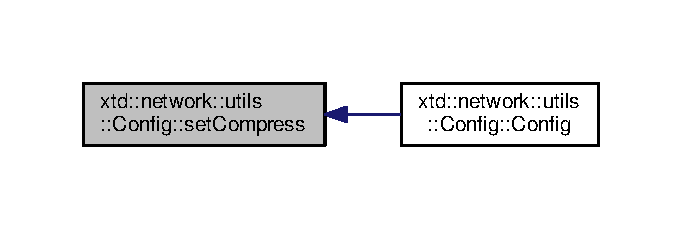
\includegraphics[width=327pt]{classxtd_1_1network_1_1utils_1_1Config_aab76e2174465ead19cc97fa3f5a7f009_icgraph}
\end{center}
\end{figure}


\index{xtd\+::network\+::utils\+::\+Config@{xtd\+::network\+::utils\+::\+Config}!set\+Compression\+Codec@{set\+Compression\+Codec}}
\index{set\+Compression\+Codec@{set\+Compression\+Codec}!xtd\+::network\+::utils\+::\+Config@{xtd\+::network\+::utils\+::\+Config}}
\subsubsection[{\texorpdfstring{set\+Compression\+Codec(codec p\+\_\+compression\+Codec)}{setCompressionCodec(codec p_compressionCodec)}}]{\setlength{\rightskip}{0pt plus 5cm}void xtd\+::network\+::utils\+::\+Config\+::set\+Compression\+Codec (
\begin{DoxyParamCaption}
\item[{{\bf codec}}]{p\+\_\+compression\+Codec}
\end{DoxyParamCaption}
)\hspace{0.3cm}{\ttfamily [inline]}}\hypertarget{classxtd_1_1network_1_1utils_1_1Config_a604e4ade1c49d83d204024f28a3d461d}{}\label{classxtd_1_1network_1_1utils_1_1Config_a604e4ade1c49d83d204024f28a3d461d}
\index{xtd\+::network\+::utils\+::\+Config@{xtd\+::network\+::utils\+::\+Config}!set\+Connect\+Timeout\+Ms@{set\+Connect\+Timeout\+Ms}}
\index{set\+Connect\+Timeout\+Ms@{set\+Connect\+Timeout\+Ms}!xtd\+::network\+::utils\+::\+Config@{xtd\+::network\+::utils\+::\+Config}}
\subsubsection[{\texorpdfstring{set\+Connect\+Timeout\+Ms(uint32\+\_\+t p\+\_\+ms)}{setConnectTimeoutMs(uint32_t p_ms)}}]{\setlength{\rightskip}{0pt plus 5cm}void xtd\+::network\+::utils\+::\+Config\+::set\+Connect\+Timeout\+Ms (
\begin{DoxyParamCaption}
\item[{uint32\+\_\+t}]{p\+\_\+ms}
\end{DoxyParamCaption}
)\hspace{0.3cm}{\ttfamily [inline]}}\hypertarget{classxtd_1_1network_1_1utils_1_1Config_a5ecd1cd77dd3bd937aa021d3bf0ad860}{}\label{classxtd_1_1network_1_1utils_1_1Config_a5ecd1cd77dd3bd937aa021d3bf0ad860}
\index{xtd\+::network\+::utils\+::\+Config@{xtd\+::network\+::utils\+::\+Config}!set\+Dns\+Cache\+T\+TL@{set\+Dns\+Cache\+T\+TL}}
\index{set\+Dns\+Cache\+T\+TL@{set\+Dns\+Cache\+T\+TL}!xtd\+::network\+::utils\+::\+Config@{xtd\+::network\+::utils\+::\+Config}}
\subsubsection[{\texorpdfstring{set\+Dns\+Cache\+T\+T\+L(uint32\+\_\+t p\+\_\+ms)}{setDnsCacheTTL(uint32_t p_ms)}}]{\setlength{\rightskip}{0pt plus 5cm}void xtd\+::network\+::utils\+::\+Config\+::set\+Dns\+Cache\+T\+TL (
\begin{DoxyParamCaption}
\item[{uint32\+\_\+t}]{p\+\_\+ms}
\end{DoxyParamCaption}
)\hspace{0.3cm}{\ttfamily [inline]}}\hypertarget{classxtd_1_1network_1_1utils_1_1Config_a9a2d3e9de6f26708a4bddc4ba7c31428}{}\label{classxtd_1_1network_1_1utils_1_1Config_a9a2d3e9de6f26708a4bddc4ba7c31428}
\index{xtd\+::network\+::utils\+::\+Config@{xtd\+::network\+::utils\+::\+Config}!set\+Linger@{set\+Linger}}
\index{set\+Linger@{set\+Linger}!xtd\+::network\+::utils\+::\+Config@{xtd\+::network\+::utils\+::\+Config}}
\subsubsection[{\texorpdfstring{set\+Linger(bool p\+\_\+linger, uint32\+\_\+t p\+\_\+linger\+Time)}{setLinger(bool p_linger, uint32_t p_lingerTime)}}]{\setlength{\rightskip}{0pt plus 5cm}void xtd\+::network\+::utils\+::\+Config\+::set\+Linger (
\begin{DoxyParamCaption}
\item[{bool}]{p\+\_\+linger, }
\item[{uint32\+\_\+t}]{p\+\_\+linger\+Time}
\end{DoxyParamCaption}
)\hspace{0.3cm}{\ttfamily [inline]}}\hypertarget{classxtd_1_1network_1_1utils_1_1Config_a1a0e52354981c89c5aaf2b31d4490de2}{}\label{classxtd_1_1network_1_1utils_1_1Config_a1a0e52354981c89c5aaf2b31d4490de2}


Here is the caller graph for this function\+:
\nopagebreak
\begin{figure}[H]
\begin{center}
\leavevmode
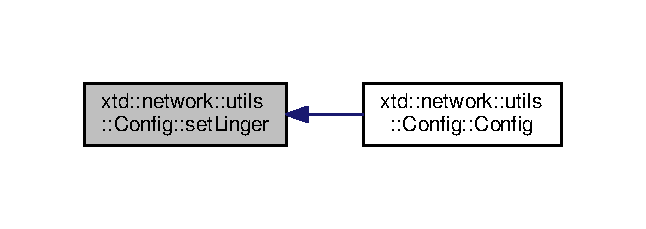
\includegraphics[width=308pt]{classxtd_1_1network_1_1utils_1_1Config_a1a0e52354981c89c5aaf2b31d4490de2_icgraph}
\end{center}
\end{figure}


\index{xtd\+::network\+::utils\+::\+Config@{xtd\+::network\+::utils\+::\+Config}!set\+No\+Delay@{set\+No\+Delay}}
\index{set\+No\+Delay@{set\+No\+Delay}!xtd\+::network\+::utils\+::\+Config@{xtd\+::network\+::utils\+::\+Config}}
\subsubsection[{\texorpdfstring{set\+No\+Delay(bool p\+\_\+no\+Delay)}{setNoDelay(bool p_noDelay)}}]{\setlength{\rightskip}{0pt plus 5cm}void xtd\+::network\+::utils\+::\+Config\+::set\+No\+Delay (
\begin{DoxyParamCaption}
\item[{bool}]{p\+\_\+no\+Delay}
\end{DoxyParamCaption}
)\hspace{0.3cm}{\ttfamily [inline]}}\hypertarget{classxtd_1_1network_1_1utils_1_1Config_a1dbcee3c0f2631269ea3e716a62ce333}{}\label{classxtd_1_1network_1_1utils_1_1Config_a1dbcee3c0f2631269ea3e716a62ce333}


Here is the caller graph for this function\+:
\nopagebreak
\begin{figure}[H]
\begin{center}
\leavevmode
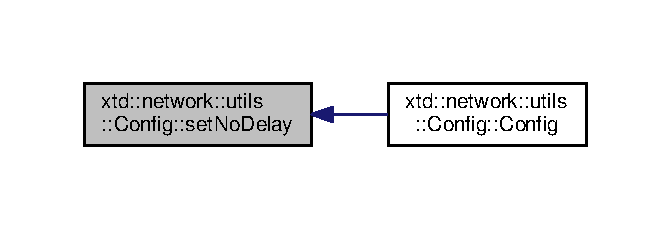
\includegraphics[width=320pt]{classxtd_1_1network_1_1utils_1_1Config_a1dbcee3c0f2631269ea3e716a62ce333_icgraph}
\end{center}
\end{figure}


\index{xtd\+::network\+::utils\+::\+Config@{xtd\+::network\+::utils\+::\+Config}!set\+Receive\+Timeout\+Ms@{set\+Receive\+Timeout\+Ms}}
\index{set\+Receive\+Timeout\+Ms@{set\+Receive\+Timeout\+Ms}!xtd\+::network\+::utils\+::\+Config@{xtd\+::network\+::utils\+::\+Config}}
\subsubsection[{\texorpdfstring{set\+Receive\+Timeout\+Ms(uint32\+\_\+t p\+\_\+ms)}{setReceiveTimeoutMs(uint32_t p_ms)}}]{\setlength{\rightskip}{0pt plus 5cm}void xtd\+::network\+::utils\+::\+Config\+::set\+Receive\+Timeout\+Ms (
\begin{DoxyParamCaption}
\item[{uint32\+\_\+t}]{p\+\_\+ms}
\end{DoxyParamCaption}
)\hspace{0.3cm}{\ttfamily [inline]}}\hypertarget{classxtd_1_1network_1_1utils_1_1Config_ad633fb35c7202550d444e4bf5ae213df}{}\label{classxtd_1_1network_1_1utils_1_1Config_ad633fb35c7202550d444e4bf5ae213df}
\index{xtd\+::network\+::utils\+::\+Config@{xtd\+::network\+::utils\+::\+Config}!set\+Reuse\+Addr@{set\+Reuse\+Addr}}
\index{set\+Reuse\+Addr@{set\+Reuse\+Addr}!xtd\+::network\+::utils\+::\+Config@{xtd\+::network\+::utils\+::\+Config}}
\subsubsection[{\texorpdfstring{set\+Reuse\+Addr(bool p\+\_\+reuse\+Addr)}{setReuseAddr(bool p_reuseAddr)}}]{\setlength{\rightskip}{0pt plus 5cm}void xtd\+::network\+::utils\+::\+Config\+::set\+Reuse\+Addr (
\begin{DoxyParamCaption}
\item[{bool}]{p\+\_\+reuse\+Addr}
\end{DoxyParamCaption}
)\hspace{0.3cm}{\ttfamily [inline]}}\hypertarget{classxtd_1_1network_1_1utils_1_1Config_a5e78cf9920484c88da5f42bae16b7a1f}{}\label{classxtd_1_1network_1_1utils_1_1Config_a5e78cf9920484c88da5f42bae16b7a1f}


Here is the caller graph for this function\+:
\nopagebreak
\begin{figure}[H]
\begin{center}
\leavevmode
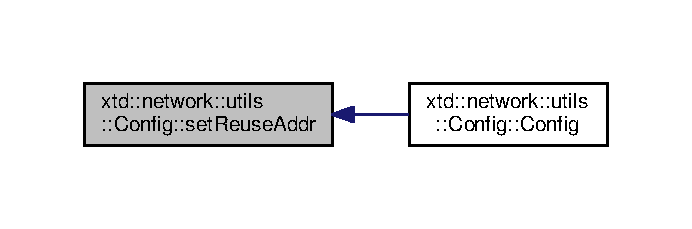
\includegraphics[width=330pt]{classxtd_1_1network_1_1utils_1_1Config_a5e78cf9920484c88da5f42bae16b7a1f_icgraph}
\end{center}
\end{figure}


\index{xtd\+::network\+::utils\+::\+Config@{xtd\+::network\+::utils\+::\+Config}!set\+Send\+Timeout\+Ms@{set\+Send\+Timeout\+Ms}}
\index{set\+Send\+Timeout\+Ms@{set\+Send\+Timeout\+Ms}!xtd\+::network\+::utils\+::\+Config@{xtd\+::network\+::utils\+::\+Config}}
\subsubsection[{\texorpdfstring{set\+Send\+Timeout\+Ms(uint32\+\_\+t p\+\_\+ms)}{setSendTimeoutMs(uint32_t p_ms)}}]{\setlength{\rightskip}{0pt plus 5cm}void xtd\+::network\+::utils\+::\+Config\+::set\+Send\+Timeout\+Ms (
\begin{DoxyParamCaption}
\item[{uint32\+\_\+t}]{p\+\_\+ms}
\end{DoxyParamCaption}
)\hspace{0.3cm}{\ttfamily [inline]}}\hypertarget{classxtd_1_1network_1_1utils_1_1Config_a583358bf6945cbddd657f6db8c31618e}{}\label{classxtd_1_1network_1_1utils_1_1Config_a583358bf6945cbddd657f6db8c31618e}


The documentation for this class was generated from the following files\+:\begin{DoxyCompactItemize}
\item 
/home/psyco/dev/xtdcpp/network/src/utils/\hyperlink{Config_8hh}{Config.\+hh}\item 
/home/psyco/dev/xtdcpp/network/src/utils/\hyperlink{Config_8cc}{Config.\+cc}\end{DoxyCompactItemize}

\hypertarget{classxtd_1_1network_1_1bip_1_1Connection}{\section{xtd\-:\-:network\-:\-:bip\-:\-:Connection$<$ Domain $>$ Class Template Reference}
\label{classxtd_1_1network_1_1bip_1_1Connection}\index{xtd\-::network\-::bip\-::\-Connection$<$ Domain $>$@{xtd\-::network\-::bip\-::\-Connection$<$ Domain $>$}}
}


{\ttfamily \#include $<$Connection.\-hh$>$}



Inheritance diagram for xtd\-:\-:network\-:\-:bip\-:\-:Connection$<$ Domain $>$\-:
\nopagebreak
\begin{figure}[H]
\begin{center}
\leavevmode
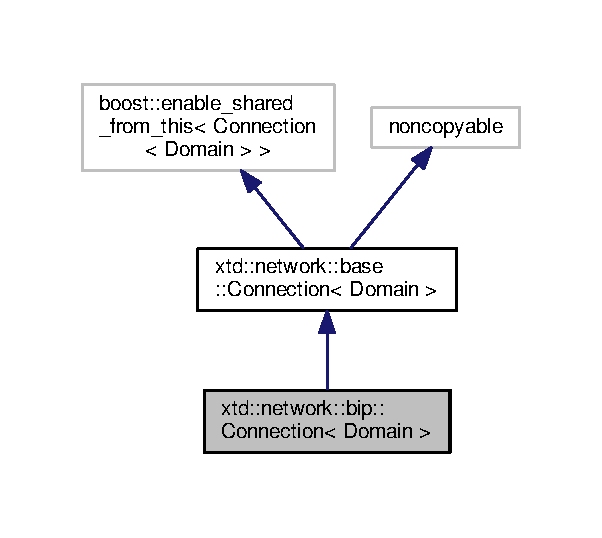
\includegraphics[width=289pt]{classxtd_1_1network_1_1bip_1_1Connection__inherit__graph}
\end{center}
\end{figure}


Collaboration diagram for xtd\-:\-:network\-:\-:bip\-:\-:Connection$<$ Domain $>$\-:
\nopagebreak
\begin{figure}[H]
\begin{center}
\leavevmode
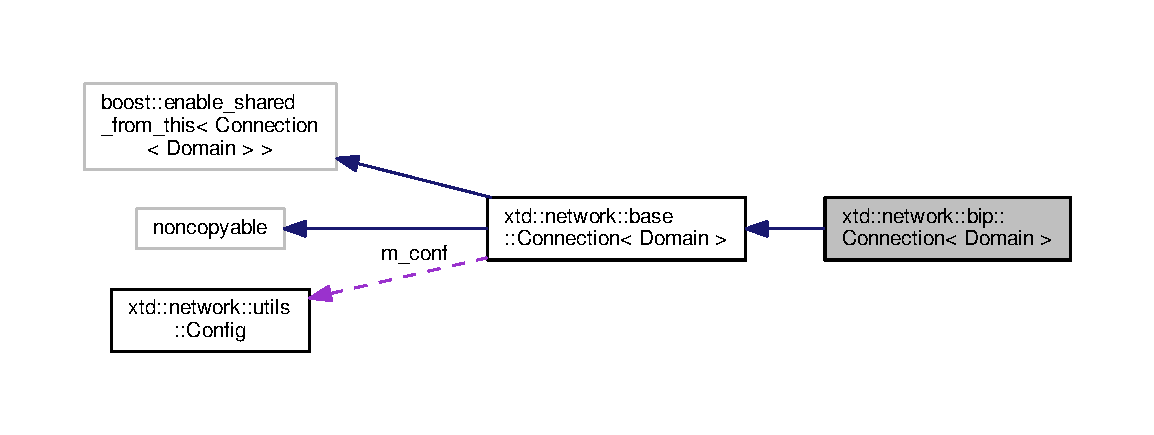
\includegraphics[width=350pt]{classxtd_1_1network_1_1bip_1_1Connection__coll__graph}
\end{center}
\end{figure}
\subsection*{Public Member Functions}
\begin{DoxyCompactItemize}
\item 
\hyperlink{classxtd_1_1network_1_1bip_1_1Connection_a5c981bbe6f8f26ac8eb25f70b2427d5c}{Connection} (const \hyperlink{classxtd_1_1network_1_1utils_1_1Config}{utils\-::\-Config} \&p\-\_\-configuration, boost\-::asio\-::io\-\_\-service \&p\-\_\-io\-Service, const string p\-\_\-hostname, const uint32\-\_\-t p\-\_\-port)
\item 
void \hyperlink{classxtd_1_1network_1_1bip_1_1Connection_acac00964a4fc76de35cdb516e9d73051}{inc\-Counter} (void)
\end{DoxyCompactItemize}
\subsection*{Additional Inherited Members}


\subsection{Detailed Description}
\subsubsection*{template$<$typename Domain$>$class xtd\-::network\-::bip\-::\-Connection$<$ Domain $>$}

\subsubsection*{Format }

Un message bip est composé de deux parties \-:
\begin{DoxyItemize}
\item un header \-: une suite de Connection\-::mcs\-\_\-header\-Size uint32\-\_\-t (donc taille fixe)
\item une data \-: une suite de taille variable de uint8
\item un crc de data \-: un crc en uint8 calculé sur les Connection\-::mcs\-\_\-max\-Data\-Crc\-Size derniers octects de la partie donnée.
\end{DoxyItemize}

Le header embarque 3 informations \-:
\begin{DoxyItemize}
\item la taille de la partie donnée (comptabilise le crc finale) en nombre d'octect
\item un identifiant de requête croissant (s'incrémente à chaque requete)
\item un crc de header calculé sur les (Connection\-::mcs\-\_\-header\-Size -\/ 1) unit32 du header
\end{DoxyItemize}

A la réception \-:
\begin{DoxyItemize}
\item on commence par lire le header
\item on vérifie l'integrité du header en comparant le crc de header reçu et le crc du header re-\/calculé
\item on extrait la taille du message N attendu a partir du header, on on va lire sur la socket ces N octects.
\end{DoxyItemize}

A la réception de la partie donnée \-:
\begin{DoxyItemize}
\item on vérifie l'intégrité du message en comparant le crc de donnée contenu dans dernier octet du message au crc recalculé.
\end{DoxyItemize}

\subsubsection*{Séquence de dialogue }

 

Definition at line 43 of file Connection.\-hh.



\subsection{Constructor \& Destructor Documentation}
\hypertarget{classxtd_1_1network_1_1bip_1_1Connection_a5c981bbe6f8f26ac8eb25f70b2427d5c}{\index{xtd\-::network\-::bip\-::\-Connection@{xtd\-::network\-::bip\-::\-Connection}!Connection@{Connection}}
\index{Connection@{Connection}!xtd::network::bip::Connection@{xtd\-::network\-::bip\-::\-Connection}}
\subsubsection[{Connection}]{\setlength{\rightskip}{0pt plus 5cm}template$<$typename Domain $>$ {\bf xtd\-::network\-::bip\-::\-Connection}$<$ Domain $>$\-::{\bf Connection} (
\begin{DoxyParamCaption}
\item[{const {\bf utils\-::\-Config} \&}]{p\-\_\-configuration, }
\item[{boost\-::asio\-::io\-\_\-service \&}]{p\-\_\-io\-Service, }
\item[{const string}]{p\-\_\-hostname, }
\item[{const uint32\-\_\-t}]{p\-\_\-port}
\end{DoxyParamCaption}
)\hspace{0.3cm}{\ttfamily [explicit]}}}\label{classxtd_1_1network_1_1bip_1_1Connection_a5c981bbe6f8f26ac8eb25f70b2427d5c}


\subsection{Member Function Documentation}
\hypertarget{classxtd_1_1network_1_1bip_1_1Connection_acac00964a4fc76de35cdb516e9d73051}{\index{xtd\-::network\-::bip\-::\-Connection@{xtd\-::network\-::bip\-::\-Connection}!inc\-Counter@{inc\-Counter}}
\index{inc\-Counter@{inc\-Counter}!xtd::network::bip::Connection@{xtd\-::network\-::bip\-::\-Connection}}
\subsubsection[{inc\-Counter}]{\setlength{\rightskip}{0pt plus 5cm}template$<$typename Domain $>$ void {\bf xtd\-::network\-::bip\-::\-Connection}$<$ Domain $>$\-::inc\-Counter (
\begin{DoxyParamCaption}
\item[{void}]{}
\end{DoxyParamCaption}
)}}\label{classxtd_1_1network_1_1bip_1_1Connection_acac00964a4fc76de35cdb516e9d73051}


The documentation for this class was generated from the following file\-:\begin{DoxyCompactItemize}
\item 
/home/travis/build/psycofdj/xtdcpp/network/src/bip/\hyperlink{bip_2Connection_8hh}{Connection.\-hh}\end{DoxyCompactItemize}

\hypertarget{classxtd_1_1network_1_1base_1_1Connection}{\section{xtd\-:\-:network\-:\-:base\-:\-:Connection$<$ Domain $>$ Class Template Reference}
\label{classxtd_1_1network_1_1base_1_1Connection}\index{xtd\-::network\-::base\-::\-Connection$<$ Domain $>$@{xtd\-::network\-::base\-::\-Connection$<$ Domain $>$}}
}


Base class from which all connections should derive.  




{\ttfamily \#include $<$Client.\-hh$>$}



Inheritance diagram for xtd\-:\-:network\-:\-:base\-:\-:Connection$<$ Domain $>$\-:
\nopagebreak
\begin{figure}[H]
\begin{center}
\leavevmode
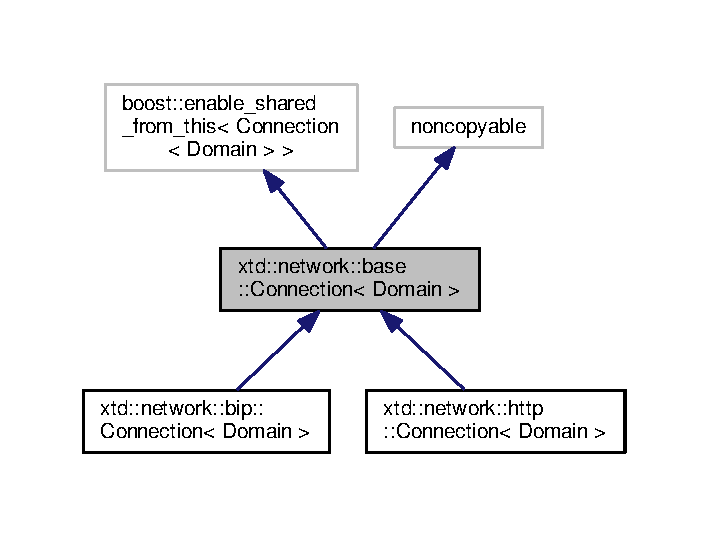
\includegraphics[width=340pt]{classxtd_1_1network_1_1base_1_1Connection__inherit__graph}
\end{center}
\end{figure}


Collaboration diagram for xtd\-:\-:network\-:\-:base\-:\-:Connection$<$ Domain $>$\-:
\nopagebreak
\begin{figure}[H]
\begin{center}
\leavevmode
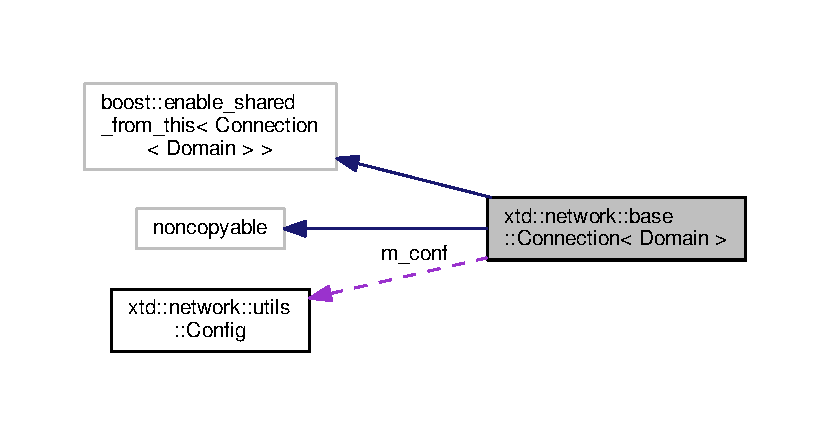
\includegraphics[width=350pt]{classxtd_1_1network_1_1base_1_1Connection__coll__graph}
\end{center}
\end{figure}
\subsection*{Public Types}
\begin{DoxyCompactItemize}
\item 
typedef boost\-::shared\-\_\-ptr\\*
$<$ \hyperlink{classxtd_1_1network_1_1base_1_1Connection}{Connection}$<$ Domain $>$ $>$ \hyperlink{classxtd_1_1network_1_1base_1_1Connection_a10f05cd689d67b012768c79486c6df47}{cnx\-\_\-sptr\-\_\-t}
\begin{DoxyCompactList}\small\item\em shared\-\_\-ptr sur this \end{DoxyCompactList}\end{DoxyCompactItemize}
\subsection*{Public Member Functions}
\begin{DoxyCompactItemize}
\item 
virtual \hyperlink{classxtd_1_1network_1_1base_1_1Connection_a51f309c311421eb6a378354914816fac}{$\sim$\-Connection} (void)
\begin{DoxyCompactList}\small\item\em descruteur \end{DoxyCompactList}\item 
void \hyperlink{classxtd_1_1network_1_1base_1_1Connection_ad5e705dc3bc5dd4e020c8caf450aab80}{set\-Process\-I\-D} (uint32\-\_\-t p\-\_\-proces\-I\-D)
\item 
uint32\-\_\-t \hyperlink{classxtd_1_1network_1_1base_1_1Connection_a5cc120a87112e3923ffc01b341ace70b}{get\-Process\-I\-D} (void) const 
\item 
void \hyperlink{classxtd_1_1network_1_1base_1_1Connection_af8da803db4caa1f125548508cf3db134}{accept} (boost\-::shared\-\_\-ptr$<$ boost\-::asio\-::basic\-\_\-socket\-\_\-acceptor$<$ Domain $>$ $>$ p\-\_\-acceptor, \hyperlink{namespacextd_1_1network_1_1utils_ac8a6f796cd645f83cde023d163665bb5}{utils\-::handler\-\_\-t} p\-\_\-on\-Accepted)
\begin{DoxyCompactList}\small\item\em ouverture aynchrone de socket (server only) \end{DoxyCompactList}\item 
void \hyperlink{classxtd_1_1network_1_1base_1_1Connection_a408b83f0e43d18e32f31d6c13d6dcdf3}{connect} (boost\-::shared\-\_\-ptr$<$ \hyperlink{classxtd_1_1network_1_1utils_1_1Resolver}{utils\-::\-Resolver}$<$ Domain $>$ $>$ p\-\_\-resolver, \hyperlink{namespacextd_1_1network_1_1utils_ac8a6f796cd645f83cde023d163665bb5}{utils\-::handler\-\_\-t} p\-\_\-on\-Connected)
\begin{DoxyCompactList}\small\item\em connexion aynchrone de socket (client only) \end{DoxyCompactList}\item 
void \hyperlink{classxtd_1_1network_1_1base_1_1Connection_a8ebc5958cf7d27a902bd75a55c4648bf}{send} (const \hyperlink{namespacextd_1_1network_1_1utils_a9fedf0d18549b8034e9ae347955e9a9a}{utils\-::vector\-Bytes\-\_\-t} \&p\-\_\-out\-Data, \hyperlink{namespacextd_1_1network_1_1utils_ac8a6f796cd645f83cde023d163665bb5}{utils\-::handler\-\_\-t} p\-\_\-on\-Sent)
\begin{DoxyCompactList}\small\item\em envoi asynchrone d'un message sur la socket \end{DoxyCompactList}\item 
void \hyperlink{classxtd_1_1network_1_1base_1_1Connection_a09146c9c2dbf1ad85867fd0afab15c0c}{receive} (\hyperlink{namespacextd_1_1network_1_1utils_a92b366b7e2a1ab09ac4f4a0401f8fb84}{utils\-::shared\-Buf\-\_\-t} p\-\_\-in\-Data, \hyperlink{namespacextd_1_1network_1_1utils_ac8a6f796cd645f83cde023d163665bb5}{utils\-::handler\-\_\-t} p\-\_\-on\-Received)
\begin{DoxyCompactList}\small\item\em reception asynchrone d'un message de la socket \end{DoxyCompactList}\item 
void \hyperlink{classxtd_1_1network_1_1base_1_1Connection_a73097d339a3716c05fee7ee19753ee4a}{close} (void)
\begin{DoxyCompactList}\small\item\em fermeture de la socket et annule ses operations de lecture ecriture \end{DoxyCompactList}\item 
void \hyperlink{classxtd_1_1network_1_1base_1_1Connection_a0bde1ab3f89862d0680c820645b7244d}{cancel} (void)
\begin{DoxyCompactList}\small\item\em annule toutes les operations asynchrones en cours de la socket \end{DoxyCompactList}\item 
const string \& \hyperlink{classxtd_1_1network_1_1base_1_1Connection_a6f249c285df79485b06f9c7b6ed03237}{info} (void) const 
\begin{DoxyCompactList}\small\item\em information de connexion (pour les logs) \end{DoxyCompactList}\end{DoxyCompactItemize}
\subsection*{Protected Member Functions}
\begin{DoxyCompactItemize}
\item 
\hyperlink{classxtd_1_1network_1_1base_1_1Connection_ac1ed59726de3423a3fc2e21e50d04542}{Connection} (const \hyperlink{classxtd_1_1network_1_1utils_1_1Config}{utils\-::\-Config} \&p\-\_\-configuration, boost\-::asio\-::io\-\_\-service \&p\-\_\-io\-Service, const string p\-\_\-hostname, const uint32\-\_\-t p\-\_\-port)
\item 
virtual void \hyperlink{classxtd_1_1network_1_1base_1_1Connection_a650bc7e13969ff9195c95307e0abb2e4}{async\-\_\-write} (\hyperlink{namespacextd_1_1network_1_1utils_a92b366b7e2a1ab09ac4f4a0401f8fb84}{utils\-::shared\-Buf\-\_\-t} p\-\_\-out\-Data, \hyperlink{namespacextd_1_1network_1_1utils_ac8a6f796cd645f83cde023d163665bb5}{utils\-::handler\-\_\-t} p\-\_\-on\-Sent)=0
\item 
virtual void \hyperlink{classxtd_1_1network_1_1base_1_1Connection_ab468f8470260b0ce42b5accf29c352e6}{async\-\_\-read} (\hyperlink{namespacextd_1_1network_1_1utils_a92b366b7e2a1ab09ac4f4a0401f8fb84}{utils\-::shared\-Buf\-\_\-t} p\-\_\-in\-Data\-Data, \hyperlink{namespacextd_1_1network_1_1utils_ac8a6f796cd645f83cde023d163665bb5}{utils\-::handler\-\_\-t} p\-\_\-on\-Received)=0
\end{DoxyCompactItemize}
\subsection*{Protected Attributes}
\begin{DoxyCompactItemize}
\item 
\hyperlink{classxtd_1_1network_1_1utils_1_1Config}{utils\-::\-Config} \hyperlink{classxtd_1_1network_1_1base_1_1Connection_a84f0cc65067a6d89a087754ad658f00b}{m\-\_\-conf}
\item 
boost\-::asio\-::io\-\_\-service \& \hyperlink{classxtd_1_1network_1_1base_1_1Connection_aee549e0f84206cc897371ec3ba2cba49}{m\-\_\-io\-Service}
\item 
boost\-::asio\-::strand \hyperlink{classxtd_1_1network_1_1base_1_1Connection_afdbd7eaed6dc0b71b05a6ef3be2f417d}{m\-\_\-strand}
\item 
boost\-::asio\-::basic\-\_\-stream\-\_\-socket\\*
$<$ Domain $>$ \hyperlink{classxtd_1_1network_1_1base_1_1Connection_af054fe7efb3d4f8a1a0f40c0e74e8c70}{m\-\_\-socket}
\end{DoxyCompactItemize}


\subsection{Detailed Description}
\subsubsection*{template$<$typename Domain$>$class xtd\-::network\-::base\-::\-Connection$<$ Domain $>$}

Base class from which all connections should derive. 


\begin{DoxyParams}{Parameters}
{\em Domain} & type de connexion \hyperlink{namespacextd_1_1network_1_1utils_a6238bab7a616eda8c9424721444a18d1}{utils\-::af\-\_\-inet} ou \hyperlink{namespacextd_1_1network_1_1utils_a60e83921a2d026f07b49fa094988acdf}{utils\-::af\-\_\-unix}\\
\hline
\end{DoxyParams}
Le premier rôle de cet objet est de mutualiser le pilotage de la socket par le client et le serveur.

Est à la charge de cet objet \-:
\begin{DoxyItemize}
\item définir les primitives asynchrones de base connect, accept, send, receive et close
\item gérer tous les contrôles d'erreur
\item gérer les timeouts
\end{DoxyItemize}

La gestion des d'erreur et des timeouts se fait en cascadant une callback locale entre le déclanchement de la callback asynchrone par le boost\-::asio\-::io\-\_\-service et la callback du client/server

Pour permettre l'implementation de tout types de prototole, cet objet n'écrit, ni ne lit directement sur la socket. Il délègue cettte tâche aux méthodes virtuelles pures \hyperlink{classxtd_1_1network_1_1base_1_1Connection_a650bc7e13969ff9195c95307e0abb2e4}{async\-\_\-write} et \hyperlink{classxtd_1_1network_1_1base_1_1Connection_ab468f8470260b0ce42b5accf29c352e6}{async\-\_\-read}.

Ces méthodes qui implémentées dans une classe fille pour chacun des protocoles. C'est typiquement là que l'on codera la création d'un header de taille fixe (ou à délimiteur fixe) qui contiendra la taille du message à lire (partie data)


\begin{DoxyItemize}
\item Thread safety \-:
\begin{DoxyItemize}
\item plusieurs instances \-: oui
\item meme instance \-: non
\end{DoxyItemize}
\item Constructeur protegé, n'a pas de sens d'utiliser cette classe telle quelle à cause des virtuelles pures
\item Bien que les primitives accept et connect ne soient pas utilisée à la fois dans le client et le server, leur implémentation a été déportée dans cet objet pour deux raisons \-:
\begin{DoxyItemize}
\item pour garantir la mise sur le strand
\item garantir l'initialisation correct des informations de socket (appel à set\-Socket\-Info qu'il faut effectuer seulement après ouverture effective de la socket) 
\end{DoxyItemize}
\end{DoxyItemize}

Definition at line 26 of file Client.\-hh.



\subsection{Member Typedef Documentation}
\hypertarget{classxtd_1_1network_1_1base_1_1Connection_a10f05cd689d67b012768c79486c6df47}{\index{xtd\-::network\-::base\-::\-Connection@{xtd\-::network\-::base\-::\-Connection}!cnx\-\_\-sptr\-\_\-t@{cnx\-\_\-sptr\-\_\-t}}
\index{cnx\-\_\-sptr\-\_\-t@{cnx\-\_\-sptr\-\_\-t}!xtd::network::base::Connection@{xtd\-::network\-::base\-::\-Connection}}
\subsubsection[{cnx\-\_\-sptr\-\_\-t}]{\setlength{\rightskip}{0pt plus 5cm}template$<$typename Domain $>$ typedef boost\-::shared\-\_\-ptr$<${\bf Connection}$<$Domain$>$ $>$ {\bf xtd\-::network\-::base\-::\-Connection}$<$ Domain $>$\-::{\bf cnx\-\_\-sptr\-\_\-t}}}\label{classxtd_1_1network_1_1base_1_1Connection_a10f05cd689d67b012768c79486c6df47}


shared\-\_\-ptr sur this 



Definition at line 62 of file Connection.\-hh.



\subsection{Constructor \& Destructor Documentation}
\hypertarget{classxtd_1_1network_1_1base_1_1Connection_ac1ed59726de3423a3fc2e21e50d04542}{\index{xtd\-::network\-::base\-::\-Connection@{xtd\-::network\-::base\-::\-Connection}!Connection@{Connection}}
\index{Connection@{Connection}!xtd::network::base::Connection@{xtd\-::network\-::base\-::\-Connection}}
\subsubsection[{Connection}]{\setlength{\rightskip}{0pt plus 5cm}template$<$typename Domain $>$ {\bf xtd\-::network\-::base\-::\-Connection}$<$ Domain $>$\-::{\bf Connection} (
\begin{DoxyParamCaption}
\item[{const {\bf utils\-::\-Config} \&}]{p\-\_\-configuration, }
\item[{boost\-::asio\-::io\-\_\-service \&}]{p\-\_\-io\-Service, }
\item[{const string}]{p\-\_\-hostname, }
\item[{const uint32\-\_\-t}]{p\-\_\-port}
\end{DoxyParamCaption}
)\hspace{0.3cm}{\ttfamily [explicit]}, {\ttfamily [protected]}}}\label{classxtd_1_1network_1_1base_1_1Connection_ac1ed59726de3423a3fc2e21e50d04542}
\hypertarget{classxtd_1_1network_1_1base_1_1Connection_a51f309c311421eb6a378354914816fac}{\index{xtd\-::network\-::base\-::\-Connection@{xtd\-::network\-::base\-::\-Connection}!$\sim$\-Connection@{$\sim$\-Connection}}
\index{$\sim$\-Connection@{$\sim$\-Connection}!xtd::network::base::Connection@{xtd\-::network\-::base\-::\-Connection}}
\subsubsection[{$\sim$\-Connection}]{\setlength{\rightskip}{0pt plus 5cm}template$<$typename Domain $>$ virtual {\bf xtd\-::network\-::base\-::\-Connection}$<$ Domain $>$\-::$\sim${\bf Connection} (
\begin{DoxyParamCaption}
\item[{void}]{}
\end{DoxyParamCaption}
)\hspace{0.3cm}{\ttfamily [virtual]}}}\label{classxtd_1_1network_1_1base_1_1Connection_a51f309c311421eb6a378354914816fac}


descruteur 



Reimplemented in \hyperlink{classxtd_1_1network_1_1http_1_1Connection_a23b8ae18927be28e3c778b1a1b23eb60}{xtd\-::network\-::http\-::\-Connection$<$ Domain $>$}.



\subsection{Member Function Documentation}
\hypertarget{classxtd_1_1network_1_1base_1_1Connection_af8da803db4caa1f125548508cf3db134}{\index{xtd\-::network\-::base\-::\-Connection@{xtd\-::network\-::base\-::\-Connection}!accept@{accept}}
\index{accept@{accept}!xtd::network::base::Connection@{xtd\-::network\-::base\-::\-Connection}}
\subsubsection[{accept}]{\setlength{\rightskip}{0pt plus 5cm}template$<$typename Domain $>$ void {\bf xtd\-::network\-::base\-::\-Connection}$<$ Domain $>$\-::accept (
\begin{DoxyParamCaption}
\item[{boost\-::shared\-\_\-ptr$<$ boost\-::asio\-::basic\-\_\-socket\-\_\-acceptor$<$ Domain $>$ $>$}]{p\-\_\-acceptor, }
\item[{{\bf utils\-::handler\-\_\-t}}]{p\-\_\-on\-Accepted}
\end{DoxyParamCaption}
)}}\label{classxtd_1_1network_1_1base_1_1Connection_af8da803db4caa1f125548508cf3db134}


ouverture aynchrone de socket (server only) 

Appel a p\-\_\-on\-Accepted lorsque l'appel aura ete execute (qu'il y ait erreur ou non)

L'acceptor est passe en parametre car c'est chez lui qu'il faut enregistré l'évenement. \hypertarget{classxtd_1_1network_1_1base_1_1Connection_ab468f8470260b0ce42b5accf29c352e6}{\index{xtd\-::network\-::base\-::\-Connection@{xtd\-::network\-::base\-::\-Connection}!async\-\_\-read@{async\-\_\-read}}
\index{async\-\_\-read@{async\-\_\-read}!xtd::network::base::Connection@{xtd\-::network\-::base\-::\-Connection}}
\subsubsection[{async\-\_\-read}]{\setlength{\rightskip}{0pt plus 5cm}template$<$typename Domain $>$ virtual void {\bf xtd\-::network\-::base\-::\-Connection}$<$ Domain $>$\-::async\-\_\-read (
\begin{DoxyParamCaption}
\item[{{\bf utils\-::shared\-Buf\-\_\-t}}]{p\-\_\-in\-Data\-Data, }
\item[{{\bf utils\-::handler\-\_\-t}}]{p\-\_\-on\-Received}
\end{DoxyParamCaption}
)\hspace{0.3cm}{\ttfamily [protected]}, {\ttfamily [pure virtual]}}}\label{classxtd_1_1network_1_1base_1_1Connection_ab468f8470260b0ce42b5accf29c352e6}
\hypertarget{classxtd_1_1network_1_1base_1_1Connection_a650bc7e13969ff9195c95307e0abb2e4}{\index{xtd\-::network\-::base\-::\-Connection@{xtd\-::network\-::base\-::\-Connection}!async\-\_\-write@{async\-\_\-write}}
\index{async\-\_\-write@{async\-\_\-write}!xtd::network::base::Connection@{xtd\-::network\-::base\-::\-Connection}}
\subsubsection[{async\-\_\-write}]{\setlength{\rightskip}{0pt plus 5cm}template$<$typename Domain $>$ virtual void {\bf xtd\-::network\-::base\-::\-Connection}$<$ Domain $>$\-::async\-\_\-write (
\begin{DoxyParamCaption}
\item[{{\bf utils\-::shared\-Buf\-\_\-t}}]{p\-\_\-out\-Data, }
\item[{{\bf utils\-::handler\-\_\-t}}]{p\-\_\-on\-Sent}
\end{DoxyParamCaption}
)\hspace{0.3cm}{\ttfamily [protected]}, {\ttfamily [pure virtual]}}}\label{classxtd_1_1network_1_1base_1_1Connection_a650bc7e13969ff9195c95307e0abb2e4}
\hypertarget{classxtd_1_1network_1_1base_1_1Connection_a0bde1ab3f89862d0680c820645b7244d}{\index{xtd\-::network\-::base\-::\-Connection@{xtd\-::network\-::base\-::\-Connection}!cancel@{cancel}}
\index{cancel@{cancel}!xtd::network::base::Connection@{xtd\-::network\-::base\-::\-Connection}}
\subsubsection[{cancel}]{\setlength{\rightskip}{0pt plus 5cm}template$<$typename Domain $>$ void {\bf xtd\-::network\-::base\-::\-Connection}$<$ Domain $>$\-::cancel (
\begin{DoxyParamCaption}
\item[{void}]{}
\end{DoxyParamCaption}
)}}\label{classxtd_1_1network_1_1base_1_1Connection_a0bde1ab3f89862d0680c820645b7244d}


annule toutes les operations asynchrones en cours de la socket 

\hypertarget{classxtd_1_1network_1_1base_1_1Connection_a73097d339a3716c05fee7ee19753ee4a}{\index{xtd\-::network\-::base\-::\-Connection@{xtd\-::network\-::base\-::\-Connection}!close@{close}}
\index{close@{close}!xtd::network::base::Connection@{xtd\-::network\-::base\-::\-Connection}}
\subsubsection[{close}]{\setlength{\rightskip}{0pt plus 5cm}template$<$typename Domain $>$ void {\bf xtd\-::network\-::base\-::\-Connection}$<$ Domain $>$\-::close (
\begin{DoxyParamCaption}
\item[{void}]{}
\end{DoxyParamCaption}
)}}\label{classxtd_1_1network_1_1base_1_1Connection_a73097d339a3716c05fee7ee19753ee4a}


fermeture de la socket et annule ses operations de lecture ecriture 

\hypertarget{classxtd_1_1network_1_1base_1_1Connection_a408b83f0e43d18e32f31d6c13d6dcdf3}{\index{xtd\-::network\-::base\-::\-Connection@{xtd\-::network\-::base\-::\-Connection}!connect@{connect}}
\index{connect@{connect}!xtd::network::base::Connection@{xtd\-::network\-::base\-::\-Connection}}
\subsubsection[{connect}]{\setlength{\rightskip}{0pt plus 5cm}template$<$typename Domain $>$ void {\bf xtd\-::network\-::base\-::\-Connection}$<$ Domain $>$\-::connect (
\begin{DoxyParamCaption}
\item[{boost\-::shared\-\_\-ptr$<$ {\bf utils\-::\-Resolver}$<$ Domain $>$ $>$}]{p\-\_\-resolver, }
\item[{{\bf utils\-::handler\-\_\-t}}]{p\-\_\-on\-Connected}
\end{DoxyParamCaption}
)}}\label{classxtd_1_1network_1_1base_1_1Connection_a408b83f0e43d18e32f31d6c13d6dcdf3}


connexion aynchrone de socket (client only) 

Appel a p\-\_\-on\-Connected lorsque l'appel aura ete execute (qu'il y ait erreur ou non) \hypertarget{classxtd_1_1network_1_1base_1_1Connection_a5cc120a87112e3923ffc01b341ace70b}{\index{xtd\-::network\-::base\-::\-Connection@{xtd\-::network\-::base\-::\-Connection}!get\-Process\-I\-D@{get\-Process\-I\-D}}
\index{get\-Process\-I\-D@{get\-Process\-I\-D}!xtd::network::base::Connection@{xtd\-::network\-::base\-::\-Connection}}
\subsubsection[{get\-Process\-I\-D}]{\setlength{\rightskip}{0pt plus 5cm}template$<$typename Domain $>$ uint32\-\_\-t {\bf xtd\-::network\-::base\-::\-Connection}$<$ Domain $>$\-::get\-Process\-I\-D (
\begin{DoxyParamCaption}
\item[{void}]{}
\end{DoxyParamCaption}
) const\hspace{0.3cm}{\ttfamily [inline]}}}\label{classxtd_1_1network_1_1base_1_1Connection_a5cc120a87112e3923ffc01b341ace70b}


Definition at line 226 of file Connection.\-hh.


\begin{DoxyCode}
227 \{
228   \textcolor{keywordflow}{return} m\_processID;
229 \}
\end{DoxyCode}
\hypertarget{classxtd_1_1network_1_1base_1_1Connection_a6f249c285df79485b06f9c7b6ed03237}{\index{xtd\-::network\-::base\-::\-Connection@{xtd\-::network\-::base\-::\-Connection}!info@{info}}
\index{info@{info}!xtd::network::base::Connection@{xtd\-::network\-::base\-::\-Connection}}
\subsubsection[{info}]{\setlength{\rightskip}{0pt plus 5cm}template$<$typename Domain $>$ const string\& {\bf xtd\-::network\-::base\-::\-Connection}$<$ Domain $>$\-::info (
\begin{DoxyParamCaption}
\item[{void}]{}
\end{DoxyParamCaption}
) const}}\label{classxtd_1_1network_1_1base_1_1Connection_a6f249c285df79485b06f9c7b6ed03237}


information de connexion (pour les logs) 

\hypertarget{classxtd_1_1network_1_1base_1_1Connection_a09146c9c2dbf1ad85867fd0afab15c0c}{\index{xtd\-::network\-::base\-::\-Connection@{xtd\-::network\-::base\-::\-Connection}!receive@{receive}}
\index{receive@{receive}!xtd::network::base::Connection@{xtd\-::network\-::base\-::\-Connection}}
\subsubsection[{receive}]{\setlength{\rightskip}{0pt plus 5cm}template$<$typename Domain $>$ void {\bf xtd\-::network\-::base\-::\-Connection}$<$ Domain $>$\-::receive (
\begin{DoxyParamCaption}
\item[{{\bf utils\-::shared\-Buf\-\_\-t}}]{p\-\_\-in\-Data, }
\item[{{\bf utils\-::handler\-\_\-t}}]{p\-\_\-on\-Received}
\end{DoxyParamCaption}
)}}\label{classxtd_1_1network_1_1base_1_1Connection_a09146c9c2dbf1ad85867fd0afab15c0c}


reception asynchrone d'un message de la socket 

Appel a p\-\_\-on\-Received lorsque l'appel aura ete execute (qu'il y ait erreur ou non) \hypertarget{classxtd_1_1network_1_1base_1_1Connection_a8ebc5958cf7d27a902bd75a55c4648bf}{\index{xtd\-::network\-::base\-::\-Connection@{xtd\-::network\-::base\-::\-Connection}!send@{send}}
\index{send@{send}!xtd::network::base::Connection@{xtd\-::network\-::base\-::\-Connection}}
\subsubsection[{send}]{\setlength{\rightskip}{0pt plus 5cm}template$<$typename Domain $>$ void {\bf xtd\-::network\-::base\-::\-Connection}$<$ Domain $>$\-::send (
\begin{DoxyParamCaption}
\item[{const {\bf utils\-::vector\-Bytes\-\_\-t} \&}]{p\-\_\-out\-Data, }
\item[{{\bf utils\-::handler\-\_\-t}}]{p\-\_\-on\-Sent}
\end{DoxyParamCaption}
)}}\label{classxtd_1_1network_1_1base_1_1Connection_a8ebc5958cf7d27a902bd75a55c4648bf}


envoi asynchrone d'un message sur la socket 

Appel a p\-\_\-on\-Sent lorsque l'appel aura ete execute (qu'il y ait erreur ou non) \hypertarget{classxtd_1_1network_1_1base_1_1Connection_ad5e705dc3bc5dd4e020c8caf450aab80}{\index{xtd\-::network\-::base\-::\-Connection@{xtd\-::network\-::base\-::\-Connection}!set\-Process\-I\-D@{set\-Process\-I\-D}}
\index{set\-Process\-I\-D@{set\-Process\-I\-D}!xtd::network::base::Connection@{xtd\-::network\-::base\-::\-Connection}}
\subsubsection[{set\-Process\-I\-D}]{\setlength{\rightskip}{0pt plus 5cm}template$<$typename Domain $>$ void {\bf xtd\-::network\-::base\-::\-Connection}$<$ Domain $>$\-::set\-Process\-I\-D (
\begin{DoxyParamCaption}
\item[{uint32\-\_\-t}]{p\-\_\-proces\-I\-D}
\end{DoxyParamCaption}
)\hspace{0.3cm}{\ttfamily [inline]}}}\label{classxtd_1_1network_1_1base_1_1Connection_ad5e705dc3bc5dd4e020c8caf450aab80}


Definition at line 219 of file Connection.\-hh.


\begin{DoxyCode}
220 \{
221   m\_processID = p\_processID;
222 \}
\end{DoxyCode}


\subsection{Member Data Documentation}
\hypertarget{classxtd_1_1network_1_1base_1_1Connection_a84f0cc65067a6d89a087754ad658f00b}{\index{xtd\-::network\-::base\-::\-Connection@{xtd\-::network\-::base\-::\-Connection}!m\-\_\-conf@{m\-\_\-conf}}
\index{m\-\_\-conf@{m\-\_\-conf}!xtd::network::base::Connection@{xtd\-::network\-::base\-::\-Connection}}
\subsubsection[{m\-\_\-conf}]{\setlength{\rightskip}{0pt plus 5cm}template$<$typename Domain $>$ {\bf utils\-::\-Config} {\bf xtd\-::network\-::base\-::\-Connection}$<$ Domain $>$\-::m\-\_\-conf\hspace{0.3cm}{\ttfamily [protected]}}}\label{classxtd_1_1network_1_1base_1_1Connection_a84f0cc65067a6d89a087754ad658f00b}


Definition at line 200 of file Connection.\-hh.

\hypertarget{classxtd_1_1network_1_1base_1_1Connection_aee549e0f84206cc897371ec3ba2cba49}{\index{xtd\-::network\-::base\-::\-Connection@{xtd\-::network\-::base\-::\-Connection}!m\-\_\-io\-Service@{m\-\_\-io\-Service}}
\index{m\-\_\-io\-Service@{m\-\_\-io\-Service}!xtd::network::base::Connection@{xtd\-::network\-::base\-::\-Connection}}
\subsubsection[{m\-\_\-io\-Service}]{\setlength{\rightskip}{0pt plus 5cm}template$<$typename Domain $>$ boost\-::asio\-::io\-\_\-service\& {\bf xtd\-::network\-::base\-::\-Connection}$<$ Domain $>$\-::m\-\_\-io\-Service\hspace{0.3cm}{\ttfamily [protected]}}}\label{classxtd_1_1network_1_1base_1_1Connection_aee549e0f84206cc897371ec3ba2cba49}


Definition at line 201 of file Connection.\-hh.

\hypertarget{classxtd_1_1network_1_1base_1_1Connection_af054fe7efb3d4f8a1a0f40c0e74e8c70}{\index{xtd\-::network\-::base\-::\-Connection@{xtd\-::network\-::base\-::\-Connection}!m\-\_\-socket@{m\-\_\-socket}}
\index{m\-\_\-socket@{m\-\_\-socket}!xtd::network::base::Connection@{xtd\-::network\-::base\-::\-Connection}}
\subsubsection[{m\-\_\-socket}]{\setlength{\rightskip}{0pt plus 5cm}template$<$typename Domain $>$ boost\-::asio\-::basic\-\_\-stream\-\_\-socket$<$Domain$>$ {\bf xtd\-::network\-::base\-::\-Connection}$<$ Domain $>$\-::m\-\_\-socket\hspace{0.3cm}{\ttfamily [protected]}}}\label{classxtd_1_1network_1_1base_1_1Connection_af054fe7efb3d4f8a1a0f40c0e74e8c70}


Definition at line 203 of file Connection.\-hh.

\hypertarget{classxtd_1_1network_1_1base_1_1Connection_afdbd7eaed6dc0b71b05a6ef3be2f417d}{\index{xtd\-::network\-::base\-::\-Connection@{xtd\-::network\-::base\-::\-Connection}!m\-\_\-strand@{m\-\_\-strand}}
\index{m\-\_\-strand@{m\-\_\-strand}!xtd::network::base::Connection@{xtd\-::network\-::base\-::\-Connection}}
\subsubsection[{m\-\_\-strand}]{\setlength{\rightskip}{0pt plus 5cm}template$<$typename Domain $>$ boost\-::asio\-::strand {\bf xtd\-::network\-::base\-::\-Connection}$<$ Domain $>$\-::m\-\_\-strand\hspace{0.3cm}{\ttfamily [protected]}}}\label{classxtd_1_1network_1_1base_1_1Connection_afdbd7eaed6dc0b71b05a6ef3be2f417d}


Definition at line 202 of file Connection.\-hh.



The documentation for this class was generated from the following files\-:\begin{DoxyCompactItemize}
\item 
/home/travis/build/psycofdj/xtdcpp/network/src/base/\hyperlink{base_2Client_8hh}{Client.\-hh}\item 
/home/travis/build/psycofdj/xtdcpp/network/src/base/\hyperlink{base_2Connection_8hh}{Connection.\-hh}\end{DoxyCompactItemize}

\hypertarget{classxtd_1_1network_1_1http_1_1Connection}{}\section{xtd\+:\+:network\+:\+:http\+:\+:Connection$<$ Domain $>$ Class Template Reference}
\label{classxtd_1_1network_1_1http_1_1Connection}\index{xtd\+::network\+::http\+::\+Connection$<$ Domain $>$@{xtd\+::network\+::http\+::\+Connection$<$ Domain $>$}}


{\ttfamily \#include $<$Connection.\+hh$>$}



Inheritance diagram for xtd\+:\+:network\+:\+:http\+:\+:Connection$<$ Domain $>$\+:
\nopagebreak
\begin{figure}[H]
\begin{center}
\leavevmode
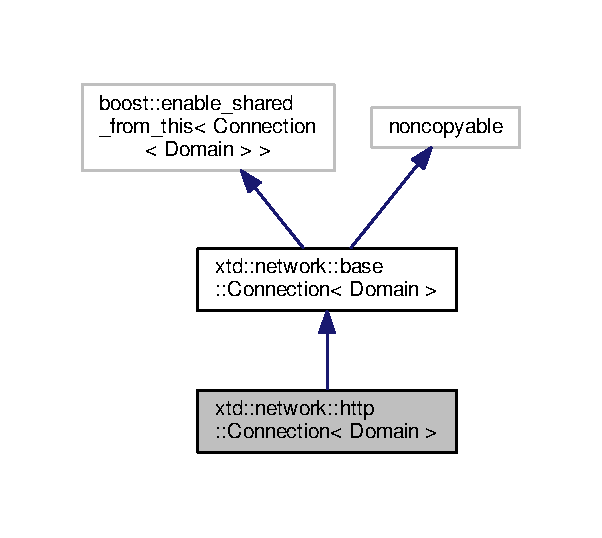
\includegraphics[width=290pt]{classxtd_1_1network_1_1http_1_1Connection__inherit__graph}
\end{center}
\end{figure}


Collaboration diagram for xtd\+:\+:network\+:\+:http\+:\+:Connection$<$ Domain $>$\+:
\nopagebreak
\begin{figure}[H]
\begin{center}
\leavevmode
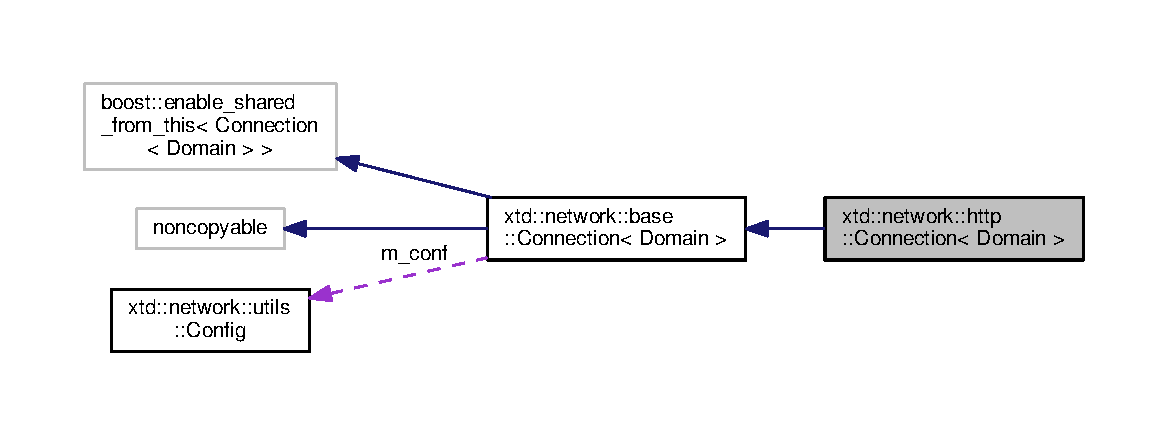
\includegraphics[width=350pt]{classxtd_1_1network_1_1http_1_1Connection__coll__graph}
\end{center}
\end{figure}
\subsection*{Public Member Functions}
\begin{DoxyCompactItemize}
\item 
\hyperlink{classxtd_1_1network_1_1http_1_1Connection_ae327f3b673c40a8481aa7e39c1bc09a4}{Connection} (const \hyperlink{classxtd_1_1network_1_1utils_1_1Config}{utils\+::\+Config} \&p\+\_\+configuration, boost\+::asio\+::io\+\_\+service \&p\+\_\+io\+Service, const string p\+\_\+hostname, const uint32\+\_\+t p\+\_\+port)
\item 
virtual \hyperlink{classxtd_1_1network_1_1http_1_1Connection_a23b8ae18927be28e3c778b1a1b23eb60}{$\sim$\+Connection} (void)
\begin{DoxyCompactList}\small\item\em descruteur \end{DoxyCompactList}\item 
void \hyperlink{classxtd_1_1network_1_1http_1_1Connection_a6bc2b4d2ca1c399b2cce22e14b52d9c4}{clear} (void)
\item 
void \hyperlink{classxtd_1_1network_1_1http_1_1Connection_a7ba68b95f6a467599c0daa93960f5821}{set\+Closed\+By\+Server} (bool p\+\_\+status)
\item 
bool \hyperlink{classxtd_1_1network_1_1http_1_1Connection_abc2998698af66ef08e5750f43e45b00f}{get\+Closed\+By\+Server} (void) const 
\end{DoxyCompactItemize}
\subsection*{Additional Inherited Members}


\subsection{Detailed Description}
\subsubsection*{template$<$typename Domain$>$\\*
class xtd\+::network\+::http\+::\+Connection$<$ Domain $>$}

Le protocol http implémenté ici gère les version 1.\+0 et une sous-\/partie de la version 1.\+1 des spécifications données par le W3C. \subsubsection*{Format}

Un message H\+T\+TP est composé de deux parties \+:
\begin{DoxyItemize}
\item un header \+: une suite de caractère ascii de taille variable terminant par une ligne vide (donc identifiable par la séquence d\textquotesingle{}octets \char`\"{}\+C\+R-\/\+L\+F-\/\+C\+R-\/\+L\+R\char`\"{})
\item une data \+: une suite de caractère ascii de taille variable, optionnelle et potentiellement encodée dans différents formats
\end{DoxyItemize}

Sans rentrer dans le détail du format du header, ce qui nous intéresse ici c\textquotesingle{}est que, lorsqu\textquotesingle{}une data est envoyée, il contient une directive {\bfseries Content-\/\+Length} qui renseigne sur la taille en octet de la data.

A la réception, on lit des données par petits bouts jusqu\textquotesingle{}à trouver la fin du header (ligne vide), on extrait ensuite la taille de la donnée et, si elle présente et est non-\/nulle, on se met à lire jusqu\textquotesingle{}à avoir suffisamment d\textquotesingle{}octets.

Pour des raisons pratique, le parsing du header et la récupération de la taille de la data est déléguée à l\textquotesingle{}objet \hyperlink{classxtd_1_1network_1_1http_1_1Request}{xtd\+::network\+::http\+::\+Request}

\subsubsection*{Séquence de dialogue }

 

Definition at line 38 of file Connection.\+hh.



\subsection{Constructor \& Destructor Documentation}
\index{xtd\+::network\+::http\+::\+Connection@{xtd\+::network\+::http\+::\+Connection}!Connection@{Connection}}
\index{Connection@{Connection}!xtd\+::network\+::http\+::\+Connection@{xtd\+::network\+::http\+::\+Connection}}
\subsubsection[{\texorpdfstring{Connection(const utils\+::\+Config \&p\+\_\+configuration, boost\+::asio\+::io\+\_\+service \&p\+\_\+io\+Service, const string p\+\_\+hostname, const uint32\+\_\+t p\+\_\+port)}{Connection(const utils::Config &p_configuration, boost::asio::io_service &p_ioService, const string p_hostname, const uint32_t p_port)}}]{\setlength{\rightskip}{0pt plus 5cm}template$<$typename Domain $>$ {\bf xtd\+::network\+::http\+::\+Connection}$<$ Domain $>$\+::{\bf Connection} (
\begin{DoxyParamCaption}
\item[{const {\bf utils\+::\+Config} \&}]{p\+\_\+configuration, }
\item[{boost\+::asio\+::io\+\_\+service \&}]{p\+\_\+io\+Service, }
\item[{const string}]{p\+\_\+hostname, }
\item[{const uint32\+\_\+t}]{p\+\_\+port}
\end{DoxyParamCaption}
)\hspace{0.3cm}{\ttfamily [explicit]}}\hypertarget{classxtd_1_1network_1_1http_1_1Connection_ae327f3b673c40a8481aa7e39c1bc09a4}{}\label{classxtd_1_1network_1_1http_1_1Connection_ae327f3b673c40a8481aa7e39c1bc09a4}
\index{xtd\+::network\+::http\+::\+Connection@{xtd\+::network\+::http\+::\+Connection}!````~Connection@{$\sim$\+Connection}}
\index{````~Connection@{$\sim$\+Connection}!xtd\+::network\+::http\+::\+Connection@{xtd\+::network\+::http\+::\+Connection}}
\subsubsection[{\texorpdfstring{$\sim$\+Connection(void)}{~Connection(void)}}]{\setlength{\rightskip}{0pt plus 5cm}template$<$typename Domain $>$ virtual {\bf xtd\+::network\+::http\+::\+Connection}$<$ Domain $>$\+::$\sim${\bf Connection} (
\begin{DoxyParamCaption}
\item[{void}]{}
\end{DoxyParamCaption}
)\hspace{0.3cm}{\ttfamily [virtual]}}\hypertarget{classxtd_1_1network_1_1http_1_1Connection_a23b8ae18927be28e3c778b1a1b23eb60}{}\label{classxtd_1_1network_1_1http_1_1Connection_a23b8ae18927be28e3c778b1a1b23eb60}


descruteur 



Reimplemented from \hyperlink{classxtd_1_1network_1_1base_1_1Connection_a51f309c311421eb6a378354914816fac}{xtd\+::network\+::base\+::\+Connection$<$ Domain $>$}.



\subsection{Member Function Documentation}
\index{xtd\+::network\+::http\+::\+Connection@{xtd\+::network\+::http\+::\+Connection}!clear@{clear}}
\index{clear@{clear}!xtd\+::network\+::http\+::\+Connection@{xtd\+::network\+::http\+::\+Connection}}
\subsubsection[{\texorpdfstring{clear(void)}{clear(void)}}]{\setlength{\rightskip}{0pt plus 5cm}template$<$typename Domain $>$ void {\bf xtd\+::network\+::http\+::\+Connection}$<$ Domain $>$\+::clear (
\begin{DoxyParamCaption}
\item[{void}]{}
\end{DoxyParamCaption}
)}\hypertarget{classxtd_1_1network_1_1http_1_1Connection_a6bc2b4d2ca1c399b2cce22e14b52d9c4}{}\label{classxtd_1_1network_1_1http_1_1Connection_a6bc2b4d2ca1c399b2cce22e14b52d9c4}
\index{xtd\+::network\+::http\+::\+Connection@{xtd\+::network\+::http\+::\+Connection}!get\+Closed\+By\+Server@{get\+Closed\+By\+Server}}
\index{get\+Closed\+By\+Server@{get\+Closed\+By\+Server}!xtd\+::network\+::http\+::\+Connection@{xtd\+::network\+::http\+::\+Connection}}
\subsubsection[{\texorpdfstring{get\+Closed\+By\+Server(void) const }{getClosedByServer(void) const }}]{\setlength{\rightskip}{0pt plus 5cm}template$<$typename Domain $>$ bool {\bf xtd\+::network\+::http\+::\+Connection}$<$ Domain $>$\+::get\+Closed\+By\+Server (
\begin{DoxyParamCaption}
\item[{void}]{}
\end{DoxyParamCaption}
) const}\hypertarget{classxtd_1_1network_1_1http_1_1Connection_abc2998698af66ef08e5750f43e45b00f}{}\label{classxtd_1_1network_1_1http_1_1Connection_abc2998698af66ef08e5750f43e45b00f}
\index{xtd\+::network\+::http\+::\+Connection@{xtd\+::network\+::http\+::\+Connection}!set\+Closed\+By\+Server@{set\+Closed\+By\+Server}}
\index{set\+Closed\+By\+Server@{set\+Closed\+By\+Server}!xtd\+::network\+::http\+::\+Connection@{xtd\+::network\+::http\+::\+Connection}}
\subsubsection[{\texorpdfstring{set\+Closed\+By\+Server(bool p\+\_\+status)}{setClosedByServer(bool p_status)}}]{\setlength{\rightskip}{0pt plus 5cm}template$<$typename Domain $>$ void {\bf xtd\+::network\+::http\+::\+Connection}$<$ Domain $>$\+::set\+Closed\+By\+Server (
\begin{DoxyParamCaption}
\item[{bool}]{p\+\_\+status}
\end{DoxyParamCaption}
)}\hypertarget{classxtd_1_1network_1_1http_1_1Connection_a7ba68b95f6a467599c0daa93960f5821}{}\label{classxtd_1_1network_1_1http_1_1Connection_a7ba68b95f6a467599c0daa93960f5821}


The documentation for this class was generated from the following file\+:\begin{DoxyCompactItemize}
\item 
/home/psyco/dev/xtdcpp/network/src/http/\hyperlink{http_2Connection_8hh}{Connection.\+hh}\end{DoxyCompactItemize}

\hypertarget{classxtd_1_1network_1_1http_1_1cpptempl_1_1Data}{}\section{xtd\+:\+:network\+:\+:http\+:\+:cpptempl\+:\+:Data Class Reference}
\label{classxtd_1_1network_1_1http_1_1cpptempl_1_1Data}\index{xtd\+::network\+::http\+::cpptempl\+::\+Data@{xtd\+::network\+::http\+::cpptempl\+::\+Data}}


{\ttfamily \#include $<$cpptempl.\+hh$>$}



Inheritance diagram for xtd\+:\+:network\+:\+:http\+:\+:cpptempl\+:\+:Data\+:
\nopagebreak
\begin{figure}[H]
\begin{center}
\leavevmode
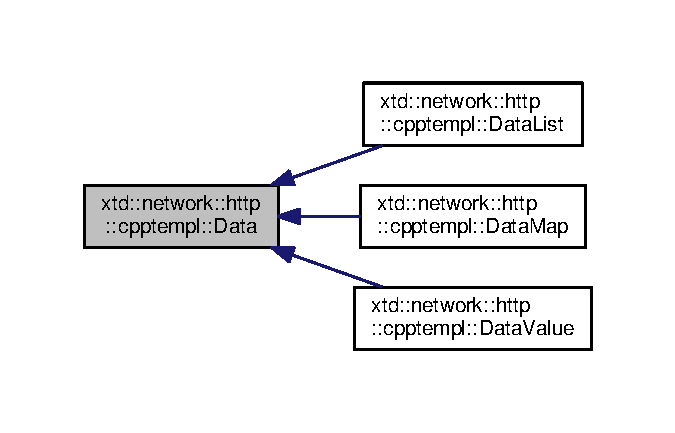
\includegraphics[width=323pt]{classxtd_1_1network_1_1http_1_1cpptempl_1_1Data__inherit__graph}
\end{center}
\end{figure}
\subsection*{Public Member Functions}
\begin{DoxyCompactItemize}
\item 
virtual \hyperlink{classxtd_1_1network_1_1http_1_1cpptempl_1_1Data_a4bbb052aa314ffb321edee297cf393e1}{$\sim$\+Data} (void)
\item 
virtual bool \hyperlink{classxtd_1_1network_1_1http_1_1cpptempl_1_1Data_a3a64cba1d65950fababffac694561af1}{empty} ()=0
\item 
virtual string \hyperlink{classxtd_1_1network_1_1http_1_1cpptempl_1_1Data_a85999dd8f43177cabf072ddbc406e556}{getvalue} ()
\item 
virtual \hyperlink{namespacextd_1_1network_1_1http_1_1cpptempl_aff1b51bcf8064f69c85dd4833c1853b4}{data\+\_\+list} \& \hyperlink{classxtd_1_1network_1_1http_1_1cpptempl_1_1Data_abb82f257b867cd0da2469cc6c5ecdbae}{getlist} ()
\item 
virtual \hyperlink{namespacextd_1_1network_1_1http_1_1cpptempl_a638d1d81c8fb63c0bbafd508d6a2a007}{data\+\_\+map} \& \hyperlink{classxtd_1_1network_1_1http_1_1cpptempl_1_1Data_a39713cc7cdc05a2375c1c5d4f00772db}{getmap} ()
\end{DoxyCompactItemize}


\subsection{Detailed Description}


Definition at line 86 of file cpptempl.\+hh.



\subsection{Constructor \& Destructor Documentation}
\index{xtd\+::network\+::http\+::cpptempl\+::\+Data@{xtd\+::network\+::http\+::cpptempl\+::\+Data}!````~Data@{$\sim$\+Data}}
\index{````~Data@{$\sim$\+Data}!xtd\+::network\+::http\+::cpptempl\+::\+Data@{xtd\+::network\+::http\+::cpptempl\+::\+Data}}
\subsubsection[{\texorpdfstring{$\sim$\+Data(void)}{~Data(void)}}]{\setlength{\rightskip}{0pt plus 5cm}virtual xtd\+::network\+::http\+::cpptempl\+::\+Data\+::$\sim$\+Data (
\begin{DoxyParamCaption}
\item[{void}]{}
\end{DoxyParamCaption}
)\hspace{0.3cm}{\ttfamily [inline]}, {\ttfamily [virtual]}}\hypertarget{classxtd_1_1network_1_1http_1_1cpptempl_1_1Data_a4bbb052aa314ffb321edee297cf393e1}{}\label{classxtd_1_1network_1_1http_1_1cpptempl_1_1Data_a4bbb052aa314ffb321edee297cf393e1}


Definition at line 89 of file cpptempl.\+hh.


\begin{DoxyCode}
89 \{\}
\end{DoxyCode}


\subsection{Member Function Documentation}
\index{xtd\+::network\+::http\+::cpptempl\+::\+Data@{xtd\+::network\+::http\+::cpptempl\+::\+Data}!empty@{empty}}
\index{empty@{empty}!xtd\+::network\+::http\+::cpptempl\+::\+Data@{xtd\+::network\+::http\+::cpptempl\+::\+Data}}
\subsubsection[{\texorpdfstring{empty()=0}{empty()=0}}]{\setlength{\rightskip}{0pt plus 5cm}virtual bool xtd\+::network\+::http\+::cpptempl\+::\+Data\+::empty (
\begin{DoxyParamCaption}
{}
\end{DoxyParamCaption}
)\hspace{0.3cm}{\ttfamily [pure virtual]}}\hypertarget{classxtd_1_1network_1_1http_1_1cpptempl_1_1Data_a3a64cba1d65950fababffac694561af1}{}\label{classxtd_1_1network_1_1http_1_1cpptempl_1_1Data_a3a64cba1d65950fababffac694561af1}


Implemented in \hyperlink{classxtd_1_1network_1_1http_1_1cpptempl_1_1DataMap_aecf13229511725a1e352f8c25fd1a40e}{xtd\+::network\+::http\+::cpptempl\+::\+Data\+Map}, \hyperlink{classxtd_1_1network_1_1http_1_1cpptempl_1_1DataList_ad495c709bd808f6864b9d4d4a3456cd8}{xtd\+::network\+::http\+::cpptempl\+::\+Data\+List}, and \hyperlink{classxtd_1_1network_1_1http_1_1cpptempl_1_1DataValue_a34a0c38c41dee41c241bd0b3141a051a}{xtd\+::network\+::http\+::cpptempl\+::\+Data\+Value}.

\index{xtd\+::network\+::http\+::cpptempl\+::\+Data@{xtd\+::network\+::http\+::cpptempl\+::\+Data}!getlist@{getlist}}
\index{getlist@{getlist}!xtd\+::network\+::http\+::cpptempl\+::\+Data@{xtd\+::network\+::http\+::cpptempl\+::\+Data}}
\subsubsection[{\texorpdfstring{getlist()}{getlist()}}]{\setlength{\rightskip}{0pt plus 5cm}{\bf data\+\_\+list} \& xtd\+::network\+::http\+::cpptempl\+::\+Data\+::getlist (
\begin{DoxyParamCaption}
{}
\end{DoxyParamCaption}
)\hspace{0.3cm}{\ttfamily [virtual]}}\hypertarget{classxtd_1_1network_1_1http_1_1cpptempl_1_1Data_abb82f257b867cd0da2469cc6c5ecdbae}{}\label{classxtd_1_1network_1_1http_1_1cpptempl_1_1Data_abb82f257b867cd0da2469cc6c5ecdbae}


Reimplemented in \hyperlink{classxtd_1_1network_1_1http_1_1cpptempl_1_1DataList_a104f3da36e9cc95c9ebb7439febe6eac}{xtd\+::network\+::http\+::cpptempl\+::\+Data\+List}.



Definition at line 18 of file cpptempl.\+cc.


\begin{DoxyCode}
19 \{
20   \textcolor{keywordflow}{throw} TemplateException(\textcolor{stringliteral}{"Data item is not a list"});
21 \}
\end{DoxyCode}
\index{xtd\+::network\+::http\+::cpptempl\+::\+Data@{xtd\+::network\+::http\+::cpptempl\+::\+Data}!getmap@{getmap}}
\index{getmap@{getmap}!xtd\+::network\+::http\+::cpptempl\+::\+Data@{xtd\+::network\+::http\+::cpptempl\+::\+Data}}
\subsubsection[{\texorpdfstring{getmap()}{getmap()}}]{\setlength{\rightskip}{0pt plus 5cm}{\bf data\+\_\+map} \& xtd\+::network\+::http\+::cpptempl\+::\+Data\+::getmap (
\begin{DoxyParamCaption}
{}
\end{DoxyParamCaption}
)\hspace{0.3cm}{\ttfamily [virtual]}}\hypertarget{classxtd_1_1network_1_1http_1_1cpptempl_1_1Data_a39713cc7cdc05a2375c1c5d4f00772db}{}\label{classxtd_1_1network_1_1http_1_1cpptempl_1_1Data_a39713cc7cdc05a2375c1c5d4f00772db}


Reimplemented in \hyperlink{classxtd_1_1network_1_1http_1_1cpptempl_1_1DataMap_abfcc73cb22b66dd0be8ad9cd66a75117}{xtd\+::network\+::http\+::cpptempl\+::\+Data\+Map}.



Definition at line 22 of file cpptempl.\+cc.


\begin{DoxyCode}
23 \{
24   \textcolor{keywordflow}{throw} TemplateException(\textcolor{stringliteral}{"Data item is not a dictionary"});
25 \}
\end{DoxyCode}
\index{xtd\+::network\+::http\+::cpptempl\+::\+Data@{xtd\+::network\+::http\+::cpptempl\+::\+Data}!getvalue@{getvalue}}
\index{getvalue@{getvalue}!xtd\+::network\+::http\+::cpptempl\+::\+Data@{xtd\+::network\+::http\+::cpptempl\+::\+Data}}
\subsubsection[{\texorpdfstring{getvalue()}{getvalue()}}]{\setlength{\rightskip}{0pt plus 5cm}string xtd\+::network\+::http\+::cpptempl\+::\+Data\+::getvalue (
\begin{DoxyParamCaption}
{}
\end{DoxyParamCaption}
)\hspace{0.3cm}{\ttfamily [virtual]}}\hypertarget{classxtd_1_1network_1_1http_1_1cpptempl_1_1Data_a85999dd8f43177cabf072ddbc406e556}{}\label{classxtd_1_1network_1_1http_1_1cpptempl_1_1Data_a85999dd8f43177cabf072ddbc406e556}


Reimplemented in \hyperlink{classxtd_1_1network_1_1http_1_1cpptempl_1_1DataValue_ad84465a538215444a2493150073941da}{xtd\+::network\+::http\+::cpptempl\+::\+Data\+Value}.



Definition at line 13 of file cpptempl.\+cc.


\begin{DoxyCode}
14 \{
15   \textcolor{keywordflow}{throw} TemplateException(\textcolor{stringliteral}{"Data item is not a value"});
16 \}
\end{DoxyCode}


The documentation for this class was generated from the following files\+:\begin{DoxyCompactItemize}
\item 
/home/psyco/dev/xtdcpp/network/src/http/\hyperlink{cpptempl_8hh}{cpptempl.\+hh}\item 
/home/psyco/dev/xtdcpp/network/src/http/\hyperlink{cpptempl_8cc}{cpptempl.\+cc}\end{DoxyCompactItemize}

\hypertarget{classxtd_1_1network_1_1http_1_1cpptempl_1_1DataList}{}\section{xtd\+:\+:network\+:\+:http\+:\+:cpptempl\+:\+:Data\+List Class Reference}
\label{classxtd_1_1network_1_1http_1_1cpptempl_1_1DataList}\index{xtd\+::network\+::http\+::cpptempl\+::\+Data\+List@{xtd\+::network\+::http\+::cpptempl\+::\+Data\+List}}


{\ttfamily \#include $<$cpptempl.\+hh$>$}



Inheritance diagram for xtd\+:\+:network\+:\+:http\+:\+:cpptempl\+:\+:Data\+List\+:
\nopagebreak
\begin{figure}[H]
\begin{center}
\leavevmode
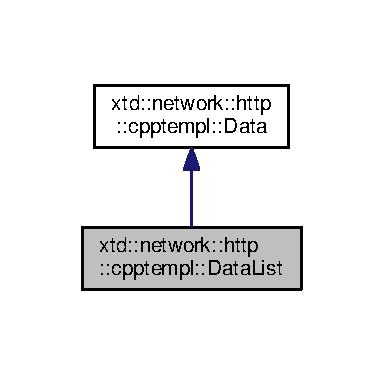
\includegraphics[width=185pt]{classxtd_1_1network_1_1http_1_1cpptempl_1_1DataList__inherit__graph}
\end{center}
\end{figure}


Collaboration diagram for xtd\+:\+:network\+:\+:http\+:\+:cpptempl\+:\+:Data\+List\+:
\nopagebreak
\begin{figure}[H]
\begin{center}
\leavevmode
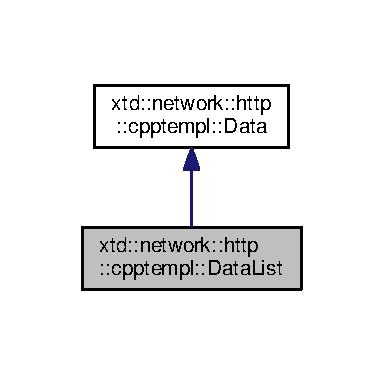
\includegraphics[width=185pt]{classxtd_1_1network_1_1http_1_1cpptempl_1_1DataList__coll__graph}
\end{center}
\end{figure}
\subsection*{Public Member Functions}
\begin{DoxyCompactItemize}
\item 
\hyperlink{classxtd_1_1network_1_1http_1_1cpptempl_1_1DataList_a0d8d86420222cd53f4316ed8ac6dfee6}{Data\+List} (\hyperlink{namespacextd_1_1network_1_1http_1_1cpptempl_aff1b51bcf8064f69c85dd4833c1853b4}{data\+\_\+list} \&items)
\item 
\hyperlink{namespacextd_1_1network_1_1http_1_1cpptempl_aff1b51bcf8064f69c85dd4833c1853b4}{data\+\_\+list} \& \hyperlink{classxtd_1_1network_1_1http_1_1cpptempl_1_1DataList_a104f3da36e9cc95c9ebb7439febe6eac}{getlist} ()
\item 
bool \hyperlink{classxtd_1_1network_1_1http_1_1cpptempl_1_1DataList_ad495c709bd808f6864b9d4d4a3456cd8}{empty} ()
\end{DoxyCompactItemize}


\subsection{Detailed Description}


Definition at line 107 of file cpptempl.\+hh.



\subsection{Constructor \& Destructor Documentation}
\index{xtd\+::network\+::http\+::cpptempl\+::\+Data\+List@{xtd\+::network\+::http\+::cpptempl\+::\+Data\+List}!Data\+List@{Data\+List}}
\index{Data\+List@{Data\+List}!xtd\+::network\+::http\+::cpptempl\+::\+Data\+List@{xtd\+::network\+::http\+::cpptempl\+::\+Data\+List}}
\subsubsection[{\texorpdfstring{Data\+List(data\+\_\+list \&items)}{DataList(data_list &items)}}]{\setlength{\rightskip}{0pt plus 5cm}xtd\+::network\+::http\+::cpptempl\+::\+Data\+List\+::\+Data\+List (
\begin{DoxyParamCaption}
\item[{{\bf data\+\_\+list} \&}]{items}
\end{DoxyParamCaption}
)\hspace{0.3cm}{\ttfamily [inline]}}\hypertarget{classxtd_1_1network_1_1http_1_1cpptempl_1_1DataList_a0d8d86420222cd53f4316ed8ac6dfee6}{}\label{classxtd_1_1network_1_1http_1_1cpptempl_1_1DataList_a0d8d86420222cd53f4316ed8ac6dfee6}


Definition at line 111 of file cpptempl.\+hh.


\begin{DoxyCode}
111 : m\_items(items)\{\}
\end{DoxyCode}


\subsection{Member Function Documentation}
\index{xtd\+::network\+::http\+::cpptempl\+::\+Data\+List@{xtd\+::network\+::http\+::cpptempl\+::\+Data\+List}!empty@{empty}}
\index{empty@{empty}!xtd\+::network\+::http\+::cpptempl\+::\+Data\+List@{xtd\+::network\+::http\+::cpptempl\+::\+Data\+List}}
\subsubsection[{\texorpdfstring{empty()}{empty()}}]{\setlength{\rightskip}{0pt plus 5cm}bool xtd\+::network\+::http\+::cpptempl\+::\+Data\+List\+::empty (
\begin{DoxyParamCaption}
{}
\end{DoxyParamCaption}
)\hspace{0.3cm}{\ttfamily [virtual]}}\hypertarget{classxtd_1_1network_1_1http_1_1cpptempl_1_1DataList_ad495c709bd808f6864b9d4d4a3456cd8}{}\label{classxtd_1_1network_1_1http_1_1cpptempl_1_1DataList_ad495c709bd808f6864b9d4d4a3456cd8}


Implements \hyperlink{classxtd_1_1network_1_1http_1_1cpptempl_1_1Data_a3a64cba1d65950fababffac694561af1}{xtd\+::network\+::http\+::cpptempl\+::\+Data}.



Definition at line 40 of file cpptempl.\+cc.


\begin{DoxyCode}
41 \{
42   \textcolor{keywordflow}{return} m\_items.empty();
43 \}
\end{DoxyCode}
\index{xtd\+::network\+::http\+::cpptempl\+::\+Data\+List@{xtd\+::network\+::http\+::cpptempl\+::\+Data\+List}!getlist@{getlist}}
\index{getlist@{getlist}!xtd\+::network\+::http\+::cpptempl\+::\+Data\+List@{xtd\+::network\+::http\+::cpptempl\+::\+Data\+List}}
\subsubsection[{\texorpdfstring{getlist()}{getlist()}}]{\setlength{\rightskip}{0pt plus 5cm}{\bf data\+\_\+list} \& xtd\+::network\+::http\+::cpptempl\+::\+Data\+List\+::getlist (
\begin{DoxyParamCaption}
{}
\end{DoxyParamCaption}
)\hspace{0.3cm}{\ttfamily [virtual]}}\hypertarget{classxtd_1_1network_1_1http_1_1cpptempl_1_1DataList_a104f3da36e9cc95c9ebb7439febe6eac}{}\label{classxtd_1_1network_1_1http_1_1cpptempl_1_1DataList_a104f3da36e9cc95c9ebb7439febe6eac}


Reimplemented from \hyperlink{classxtd_1_1network_1_1http_1_1cpptempl_1_1Data_abb82f257b867cd0da2469cc6c5ecdbae}{xtd\+::network\+::http\+::cpptempl\+::\+Data}.



Definition at line 35 of file cpptempl.\+cc.


\begin{DoxyCode}
36 \{
37   \textcolor{keywordflow}{return} m\_items;
38 \}
\end{DoxyCode}


The documentation for this class was generated from the following files\+:\begin{DoxyCompactItemize}
\item 
/home/psyco/dev/xtdcpp/network/src/http/\hyperlink{cpptempl_8hh}{cpptempl.\+hh}\item 
/home/psyco/dev/xtdcpp/network/src/http/\hyperlink{cpptempl_8cc}{cpptempl.\+cc}\end{DoxyCompactItemize}

\hypertarget{classxtd_1_1network_1_1http_1_1cpptempl_1_1DataMap}{\section{xtd\-:\-:network\-:\-:http\-:\-:cpptempl\-:\-:Data\-Map Class Reference}
\label{classxtd_1_1network_1_1http_1_1cpptempl_1_1DataMap}\index{xtd\-::network\-::http\-::cpptempl\-::\-Data\-Map@{xtd\-::network\-::http\-::cpptempl\-::\-Data\-Map}}
}


{\ttfamily \#include $<$cpptempl.\-hh$>$}



Inheritance diagram for xtd\-:\-:network\-:\-:http\-:\-:cpptempl\-:\-:Data\-Map\-:
\nopagebreak
\begin{figure}[H]
\begin{center}
\leavevmode
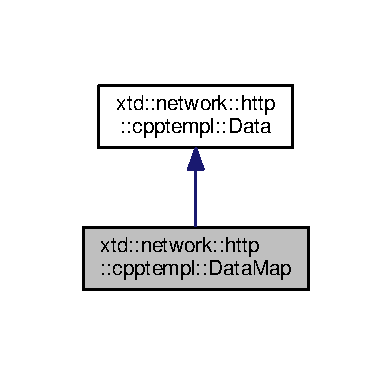
\includegraphics[width=188pt]{classxtd_1_1network_1_1http_1_1cpptempl_1_1DataMap__inherit__graph}
\end{center}
\end{figure}


Collaboration diagram for xtd\-:\-:network\-:\-:http\-:\-:cpptempl\-:\-:Data\-Map\-:
\nopagebreak
\begin{figure}[H]
\begin{center}
\leavevmode
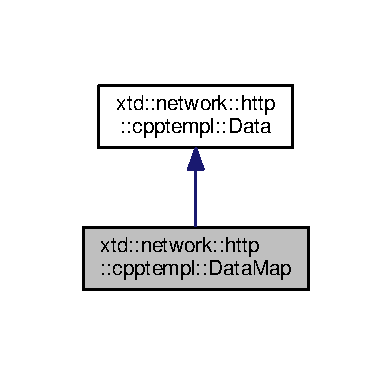
\includegraphics[width=188pt]{classxtd_1_1network_1_1http_1_1cpptempl_1_1DataMap__coll__graph}
\end{center}
\end{figure}
\subsection*{Public Member Functions}
\begin{DoxyCompactItemize}
\item 
\hyperlink{classxtd_1_1network_1_1http_1_1cpptempl_1_1DataMap_a9a5267694ba26050526a02407c69937f}{Data\-Map} (\hyperlink{namespacextd_1_1network_1_1http_1_1cpptempl_a638d1d81c8fb63c0bbafd508d6a2a007}{data\-\_\-map} \&items)
\item 
\hyperlink{namespacextd_1_1network_1_1http_1_1cpptempl_a638d1d81c8fb63c0bbafd508d6a2a007}{data\-\_\-map} \& \hyperlink{classxtd_1_1network_1_1http_1_1cpptempl_1_1DataMap_abfcc73cb22b66dd0be8ad9cd66a75117}{getmap} ()
\item 
bool \hyperlink{classxtd_1_1network_1_1http_1_1cpptempl_1_1DataMap_aecf13229511725a1e352f8c25fd1a40e}{empty} ()
\end{DoxyCompactItemize}


\subsection{Detailed Description}


Definition at line 117 of file cpptempl.\-hh.



\subsection{Constructor \& Destructor Documentation}
\hypertarget{classxtd_1_1network_1_1http_1_1cpptempl_1_1DataMap_a9a5267694ba26050526a02407c69937f}{\index{xtd\-::network\-::http\-::cpptempl\-::\-Data\-Map@{xtd\-::network\-::http\-::cpptempl\-::\-Data\-Map}!Data\-Map@{Data\-Map}}
\index{Data\-Map@{Data\-Map}!xtd::network::http::cpptempl::DataMap@{xtd\-::network\-::http\-::cpptempl\-::\-Data\-Map}}
\subsubsection[{Data\-Map}]{\setlength{\rightskip}{0pt plus 5cm}xtd\-::network\-::http\-::cpptempl\-::\-Data\-Map\-::\-Data\-Map (
\begin{DoxyParamCaption}
\item[{{\bf data\-\_\-map} \&}]{items}
\end{DoxyParamCaption}
)\hspace{0.3cm}{\ttfamily [inline]}}}\label{classxtd_1_1network_1_1http_1_1cpptempl_1_1DataMap_a9a5267694ba26050526a02407c69937f}


Definition at line 121 of file cpptempl.\-hh.


\begin{DoxyCode}
121 : m\_items(items)\{\}
\end{DoxyCode}


\subsection{Member Function Documentation}
\hypertarget{classxtd_1_1network_1_1http_1_1cpptempl_1_1DataMap_aecf13229511725a1e352f8c25fd1a40e}{\index{xtd\-::network\-::http\-::cpptempl\-::\-Data\-Map@{xtd\-::network\-::http\-::cpptempl\-::\-Data\-Map}!empty@{empty}}
\index{empty@{empty}!xtd::network::http::cpptempl::DataMap@{xtd\-::network\-::http\-::cpptempl\-::\-Data\-Map}}
\subsubsection[{empty}]{\setlength{\rightskip}{0pt plus 5cm}bool xtd\-::network\-::http\-::cpptempl\-::\-Data\-Map\-::empty (
\begin{DoxyParamCaption}
{}
\end{DoxyParamCaption}
)\hspace{0.3cm}{\ttfamily [virtual]}}}\label{classxtd_1_1network_1_1http_1_1cpptempl_1_1DataMap_aecf13229511725a1e352f8c25fd1a40e}


Implements \hyperlink{classxtd_1_1network_1_1http_1_1cpptempl_1_1Data_a3a64cba1d65950fababffac694561af1}{xtd\-::network\-::http\-::cpptempl\-::\-Data}.



Definition at line 49 of file cpptempl.\-cc.


\begin{DoxyCode}
50 \{
51   \textcolor{keywordflow}{return} m\_items.empty();
52 \}
\end{DoxyCode}
\hypertarget{classxtd_1_1network_1_1http_1_1cpptempl_1_1DataMap_abfcc73cb22b66dd0be8ad9cd66a75117}{\index{xtd\-::network\-::http\-::cpptempl\-::\-Data\-Map@{xtd\-::network\-::http\-::cpptempl\-::\-Data\-Map}!getmap@{getmap}}
\index{getmap@{getmap}!xtd::network::http::cpptempl::DataMap@{xtd\-::network\-::http\-::cpptempl\-::\-Data\-Map}}
\subsubsection[{getmap}]{\setlength{\rightskip}{0pt plus 5cm}{\bf data\-\_\-map} \& xtd\-::network\-::http\-::cpptempl\-::\-Data\-Map\-::getmap (
\begin{DoxyParamCaption}
{}
\end{DoxyParamCaption}
)\hspace{0.3cm}{\ttfamily [virtual]}}}\label{classxtd_1_1network_1_1http_1_1cpptempl_1_1DataMap_abfcc73cb22b66dd0be8ad9cd66a75117}


Reimplemented from \hyperlink{classxtd_1_1network_1_1http_1_1cpptempl_1_1Data_a39713cc7cdc05a2375c1c5d4f00772db}{xtd\-::network\-::http\-::cpptempl\-::\-Data}.



Definition at line 44 of file cpptempl.\-cc.


\begin{DoxyCode}
45 \{
46   \textcolor{keywordflow}{return} m\_items;
47 \}
\end{DoxyCode}


The documentation for this class was generated from the following files\-:\begin{DoxyCompactItemize}
\item 
/home/travis/build/psycofdj/xtdcpp/network/src/http/\hyperlink{cpptempl_8hh}{cpptempl.\-hh}\item 
/home/travis/build/psycofdj/xtdcpp/network/src/http/\hyperlink{cpptempl_8cc}{cpptempl.\-cc}\end{DoxyCompactItemize}

\hypertarget{classxtd_1_1network_1_1http_1_1cpptempl_1_1DataValue}{}\section{xtd\+:\+:network\+:\+:http\+:\+:cpptempl\+:\+:Data\+Value Class Reference}
\label{classxtd_1_1network_1_1http_1_1cpptempl_1_1DataValue}\index{xtd\+::network\+::http\+::cpptempl\+::\+Data\+Value@{xtd\+::network\+::http\+::cpptempl\+::\+Data\+Value}}


{\ttfamily \#include $<$cpptempl.\+hh$>$}



Inheritance diagram for xtd\+:\+:network\+:\+:http\+:\+:cpptempl\+:\+:Data\+Value\+:
\nopagebreak
\begin{figure}[H]
\begin{center}
\leavevmode
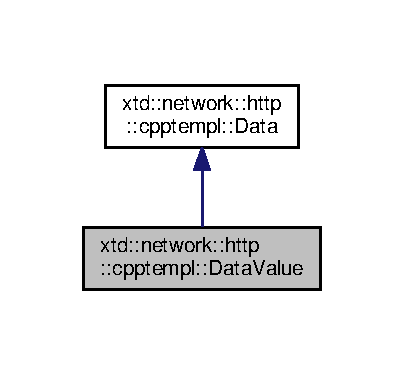
\includegraphics[width=194pt]{classxtd_1_1network_1_1http_1_1cpptempl_1_1DataValue__inherit__graph}
\end{center}
\end{figure}


Collaboration diagram for xtd\+:\+:network\+:\+:http\+:\+:cpptempl\+:\+:Data\+Value\+:
\nopagebreak
\begin{figure}[H]
\begin{center}
\leavevmode
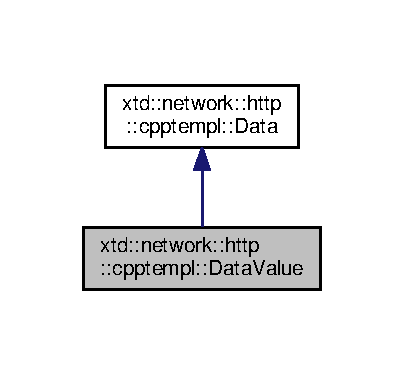
\includegraphics[width=194pt]{classxtd_1_1network_1_1http_1_1cpptempl_1_1DataValue__coll__graph}
\end{center}
\end{figure}
\subsection*{Public Member Functions}
\begin{DoxyCompactItemize}
\item 
\hyperlink{classxtd_1_1network_1_1http_1_1cpptempl_1_1DataValue_a51718755a978b1cb88039e3f192c61f2}{Data\+Value} (string value)
\item 
string \hyperlink{classxtd_1_1network_1_1http_1_1cpptempl_1_1DataValue_ad84465a538215444a2493150073941da}{getvalue} ()
\item 
bool \hyperlink{classxtd_1_1network_1_1http_1_1cpptempl_1_1DataValue_a34a0c38c41dee41c241bd0b3141a051a}{empty} ()
\end{DoxyCompactItemize}


\subsection{Detailed Description}


Definition at line 97 of file cpptempl.\+hh.



\subsection{Constructor \& Destructor Documentation}
\index{xtd\+::network\+::http\+::cpptempl\+::\+Data\+Value@{xtd\+::network\+::http\+::cpptempl\+::\+Data\+Value}!Data\+Value@{Data\+Value}}
\index{Data\+Value@{Data\+Value}!xtd\+::network\+::http\+::cpptempl\+::\+Data\+Value@{xtd\+::network\+::http\+::cpptempl\+::\+Data\+Value}}
\subsubsection[{\texorpdfstring{Data\+Value(string value)}{DataValue(string value)}}]{\setlength{\rightskip}{0pt plus 5cm}xtd\+::network\+::http\+::cpptempl\+::\+Data\+Value\+::\+Data\+Value (
\begin{DoxyParamCaption}
\item[{string}]{value}
\end{DoxyParamCaption}
)\hspace{0.3cm}{\ttfamily [inline]}}\hypertarget{classxtd_1_1network_1_1http_1_1cpptempl_1_1DataValue_a51718755a978b1cb88039e3f192c61f2}{}\label{classxtd_1_1network_1_1http_1_1cpptempl_1_1DataValue_a51718755a978b1cb88039e3f192c61f2}


Definition at line 101 of file cpptempl.\+hh.


\begin{DoxyCode}
101 : m\_value(value)\{\}
\end{DoxyCode}


\subsection{Member Function Documentation}
\index{xtd\+::network\+::http\+::cpptempl\+::\+Data\+Value@{xtd\+::network\+::http\+::cpptempl\+::\+Data\+Value}!empty@{empty}}
\index{empty@{empty}!xtd\+::network\+::http\+::cpptempl\+::\+Data\+Value@{xtd\+::network\+::http\+::cpptempl\+::\+Data\+Value}}
\subsubsection[{\texorpdfstring{empty()}{empty()}}]{\setlength{\rightskip}{0pt plus 5cm}bool xtd\+::network\+::http\+::cpptempl\+::\+Data\+Value\+::empty (
\begin{DoxyParamCaption}
{}
\end{DoxyParamCaption}
)\hspace{0.3cm}{\ttfamily [virtual]}}\hypertarget{classxtd_1_1network_1_1http_1_1cpptempl_1_1DataValue_a34a0c38c41dee41c241bd0b3141a051a}{}\label{classxtd_1_1network_1_1http_1_1cpptempl_1_1DataValue_a34a0c38c41dee41c241bd0b3141a051a}


Implements \hyperlink{classxtd_1_1network_1_1http_1_1cpptempl_1_1Data_a3a64cba1d65950fababffac694561af1}{xtd\+::network\+::http\+::cpptempl\+::\+Data}.



Definition at line 31 of file cpptempl.\+cc.


\begin{DoxyCode}
32 \{
33   \textcolor{keywordflow}{return} m\_value.empty();
34 \}
\end{DoxyCode}
\index{xtd\+::network\+::http\+::cpptempl\+::\+Data\+Value@{xtd\+::network\+::http\+::cpptempl\+::\+Data\+Value}!getvalue@{getvalue}}
\index{getvalue@{getvalue}!xtd\+::network\+::http\+::cpptempl\+::\+Data\+Value@{xtd\+::network\+::http\+::cpptempl\+::\+Data\+Value}}
\subsubsection[{\texorpdfstring{getvalue()}{getvalue()}}]{\setlength{\rightskip}{0pt plus 5cm}string xtd\+::network\+::http\+::cpptempl\+::\+Data\+Value\+::getvalue (
\begin{DoxyParamCaption}
{}
\end{DoxyParamCaption}
)\hspace{0.3cm}{\ttfamily [virtual]}}\hypertarget{classxtd_1_1network_1_1http_1_1cpptempl_1_1DataValue_ad84465a538215444a2493150073941da}{}\label{classxtd_1_1network_1_1http_1_1cpptempl_1_1DataValue_ad84465a538215444a2493150073941da}


Reimplemented from \hyperlink{classxtd_1_1network_1_1http_1_1cpptempl_1_1Data_a85999dd8f43177cabf072ddbc406e556}{xtd\+::network\+::http\+::cpptempl\+::\+Data}.



Definition at line 26 of file cpptempl.\+cc.


\begin{DoxyCode}
27 \{
28   \textcolor{keywordflow}{return} m\_value;
29 \}
\end{DoxyCode}


The documentation for this class was generated from the following files\+:\begin{DoxyCompactItemize}
\item 
/home/psyco/dev/xtdcpp/network/src/http/\hyperlink{cpptempl_8hh}{cpptempl.\+hh}\item 
/home/psyco/dev/xtdcpp/network/src/http/\hyperlink{cpptempl_8cc}{cpptempl.\+cc}\end{DoxyCompactItemize}

\hypertarget{classxtd_1_1network_1_1utils_1_1deque__id}{\section{xtd\-:\-:network\-:\-:utils\-:\-:deque\-\_\-id$<$ T $>$ Class Template Reference}
\label{classxtd_1_1network_1_1utils_1_1deque__id}\index{xtd\-::network\-::utils\-::deque\-\_\-id$<$ T $>$@{xtd\-::network\-::utils\-::deque\-\_\-id$<$ T $>$}}
}


{\ttfamily \#include $<$Utils.\-hh$>$}

\subsection*{Public Member Functions}
\begin{DoxyCompactItemize}
\item 
void \hyperlink{classxtd_1_1network_1_1utils_1_1deque__id_ace5bd507db72397f457723944c21b575}{push} (const T \&p\-\_\-param)
\item 
void \hyperlink{classxtd_1_1network_1_1utils_1_1deque__id_ae947d106bc8943450c1eab9df3880401}{push\-\_\-back} (const T \&p\-\_\-param)
\item 
bool \hyperlink{classxtd_1_1network_1_1utils_1_1deque__id_a4d61e0412fbc4bb454141e8f760d191b}{pop} (T \&p\-\_\-param)
\item 
bool \hyperlink{classxtd_1_1network_1_1utils_1_1deque__id_ad18ee554089fe3016e1dd4c7b363c6a8}{find} (const T \&p\-\_\-param)
\item 
size\-\_\-t \hyperlink{classxtd_1_1network_1_1utils_1_1deque__id_a6038f59387bc5dcffb339b0d8c9424fa}{size} (void)
\end{DoxyCompactItemize}


\subsection{Detailed Description}
\subsubsection*{template$<$typename T$>$class xtd\-::network\-::utils\-::deque\-\_\-id$<$ T $>$}



Definition at line 40 of file Utils.\-hh.



\subsection{Member Function Documentation}
\hypertarget{classxtd_1_1network_1_1utils_1_1deque__id_ad18ee554089fe3016e1dd4c7b363c6a8}{\index{xtd\-::network\-::utils\-::deque\-\_\-id@{xtd\-::network\-::utils\-::deque\-\_\-id}!find@{find}}
\index{find@{find}!xtd::network::utils::deque_id@{xtd\-::network\-::utils\-::deque\-\_\-id}}
\subsubsection[{find}]{\setlength{\rightskip}{0pt plus 5cm}template$<$typename T$>$ bool {\bf xtd\-::network\-::utils\-::deque\-\_\-id}$<$ T $>$\-::find (
\begin{DoxyParamCaption}
\item[{const T \&}]{p\-\_\-param}
\end{DoxyParamCaption}
)}}\label{classxtd_1_1network_1_1utils_1_1deque__id_ad18ee554089fe3016e1dd4c7b363c6a8}
\hypertarget{classxtd_1_1network_1_1utils_1_1deque__id_a4d61e0412fbc4bb454141e8f760d191b}{\index{xtd\-::network\-::utils\-::deque\-\_\-id@{xtd\-::network\-::utils\-::deque\-\_\-id}!pop@{pop}}
\index{pop@{pop}!xtd::network::utils::deque_id@{xtd\-::network\-::utils\-::deque\-\_\-id}}
\subsubsection[{pop}]{\setlength{\rightskip}{0pt plus 5cm}template$<$typename T$>$ bool {\bf xtd\-::network\-::utils\-::deque\-\_\-id}$<$ T $>$\-::pop (
\begin{DoxyParamCaption}
\item[{T \&}]{p\-\_\-param}
\end{DoxyParamCaption}
)}}\label{classxtd_1_1network_1_1utils_1_1deque__id_a4d61e0412fbc4bb454141e8f760d191b}
\hypertarget{classxtd_1_1network_1_1utils_1_1deque__id_ace5bd507db72397f457723944c21b575}{\index{xtd\-::network\-::utils\-::deque\-\_\-id@{xtd\-::network\-::utils\-::deque\-\_\-id}!push@{push}}
\index{push@{push}!xtd::network::utils::deque_id@{xtd\-::network\-::utils\-::deque\-\_\-id}}
\subsubsection[{push}]{\setlength{\rightskip}{0pt plus 5cm}template$<$typename T$>$ void {\bf xtd\-::network\-::utils\-::deque\-\_\-id}$<$ T $>$\-::push (
\begin{DoxyParamCaption}
\item[{const T \&}]{p\-\_\-param}
\end{DoxyParamCaption}
)}}\label{classxtd_1_1network_1_1utils_1_1deque__id_ace5bd507db72397f457723944c21b575}
\hypertarget{classxtd_1_1network_1_1utils_1_1deque__id_ae947d106bc8943450c1eab9df3880401}{\index{xtd\-::network\-::utils\-::deque\-\_\-id@{xtd\-::network\-::utils\-::deque\-\_\-id}!push\-\_\-back@{push\-\_\-back}}
\index{push\-\_\-back@{push\-\_\-back}!xtd::network::utils::deque_id@{xtd\-::network\-::utils\-::deque\-\_\-id}}
\subsubsection[{push\-\_\-back}]{\setlength{\rightskip}{0pt plus 5cm}template$<$typename T$>$ void {\bf xtd\-::network\-::utils\-::deque\-\_\-id}$<$ T $>$\-::push\-\_\-back (
\begin{DoxyParamCaption}
\item[{const T \&}]{p\-\_\-param}
\end{DoxyParamCaption}
)}}\label{classxtd_1_1network_1_1utils_1_1deque__id_ae947d106bc8943450c1eab9df3880401}
\hypertarget{classxtd_1_1network_1_1utils_1_1deque__id_a6038f59387bc5dcffb339b0d8c9424fa}{\index{xtd\-::network\-::utils\-::deque\-\_\-id@{xtd\-::network\-::utils\-::deque\-\_\-id}!size@{size}}
\index{size@{size}!xtd::network::utils::deque_id@{xtd\-::network\-::utils\-::deque\-\_\-id}}
\subsubsection[{size}]{\setlength{\rightskip}{0pt plus 5cm}template$<$typename T$>$ size\-\_\-t {\bf xtd\-::network\-::utils\-::deque\-\_\-id}$<$ T $>$\-::size (
\begin{DoxyParamCaption}
\item[{void}]{}
\end{DoxyParamCaption}
)}}\label{classxtd_1_1network_1_1utils_1_1deque__id_a6038f59387bc5dcffb339b0d8c9424fa}


The documentation for this class was generated from the following file\-:\begin{DoxyCompactItemize}
\item 
/home/travis/build/psycofdj/xtdcpp/network/src/utils/\hyperlink{Utils_8hh}{Utils.\-hh}\end{DoxyCompactItemize}

\hypertarget{structxtd_1_1network_1_1http_1_1Server_1_1Handler_1_1filter}{}\section{xtd\+:\+:network\+:\+:http\+:\+:Server$<$ Domain $>$\+:\+:Handler\+:\+:filter Struct Reference}
\label{structxtd_1_1network_1_1http_1_1Server_1_1Handler_1_1filter}\index{xtd\+::network\+::http\+::\+Server$<$ Domain $>$\+::\+Handler\+::filter@{xtd\+::network\+::http\+::\+Server$<$ Domain $>$\+::\+Handler\+::filter}}


{\ttfamily \#include $<$Server.\+hh$>$}



Inheritance diagram for xtd\+:\+:network\+:\+:http\+:\+:Server$<$ Domain $>$\+:\+:Handler\+:\+:filter\+:
\nopagebreak
\begin{figure}[H]
\begin{center}
\leavevmode
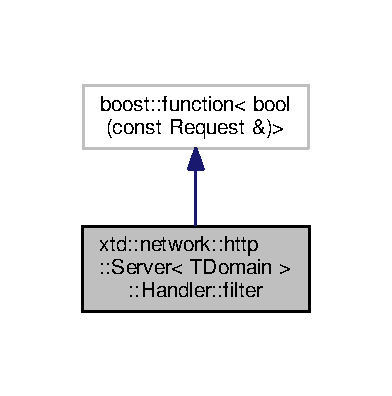
\includegraphics[width=189pt]{structxtd_1_1network_1_1http_1_1Server_1_1Handler_1_1filter__inherit__graph}
\end{center}
\end{figure}


Collaboration diagram for xtd\+:\+:network\+:\+:http\+:\+:Server$<$ Domain $>$\+:\+:Handler\+:\+:filter\+:
\nopagebreak
\begin{figure}[H]
\begin{center}
\leavevmode
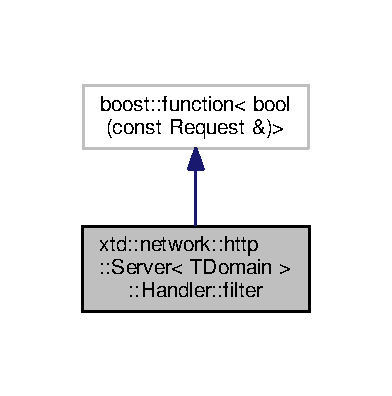
\includegraphics[width=189pt]{structxtd_1_1network_1_1http_1_1Server_1_1Handler_1_1filter__coll__graph}
\end{center}
\end{figure}
\subsection*{Public Types}
\begin{DoxyCompactItemize}
\item 
typedef boost\+::function$<$ bool(const \hyperlink{classxtd_1_1network_1_1http_1_1Request}{Request} \&)$>$ \hyperlink{structxtd_1_1network_1_1http_1_1Server_1_1Handler_1_1filter_a7a443c95291e03dff64632da70c3970e}{t\+\_\+func}
\end{DoxyCompactItemize}
\subsection*{Public Member Functions}
\begin{DoxyCompactItemize}
\item 
\hyperlink{structxtd_1_1network_1_1http_1_1Server_1_1Handler_1_1filter_aade4e97fe12a8e43c647ac1ca7cc21c7}{filter} (void)
\item 
{\footnotesize template$<$class A $>$ }\\\hyperlink{structxtd_1_1network_1_1http_1_1Server_1_1Handler_1_1filter_af56d192d61507e75ff21f4f075df1bd3}{filter} (A p\+\_\+method)
\item 
{\footnotesize template$<$class A , typename Base $>$ }\\\hyperlink{structxtd_1_1network_1_1http_1_1Server_1_1Handler_1_1filter_a47da45a50b8b22c1a141d1602ac9f9eb}{filter} (A p\+\_\+method, Base p\+\_\+instance)
\item 
{\footnotesize template$<$class A , typename Base , typename B $>$ }\\\hyperlink{structxtd_1_1network_1_1http_1_1Server_1_1Handler_1_1filter_a4882bb6111bfa1007238091519723432}{filter} (A p\+\_\+method, Base p\+\_\+instance, B p\+\_\+arg1)
\item 
{\footnotesize template$<$class A , typename Base , typename B , typename C $>$ }\\\hyperlink{structxtd_1_1network_1_1http_1_1Server_1_1Handler_1_1filter_a9caa6426ff014b29d856845e542ecc61}{filter} (A p\+\_\+method, Base p\+\_\+instance, B p\+\_\+arg1, C p\+\_\+arg2)
\item 
{\footnotesize template$<$class A , typename Base , typename B , typename C , typename D $>$ }\\\hyperlink{structxtd_1_1network_1_1http_1_1Server_1_1Handler_1_1filter_aa73bc46ea27365b04dabc4ad3883f6e3}{filter} (A p\+\_\+method, Base p\+\_\+instance, B p\+\_\+arg1, C p\+\_\+arg2, D p\+\_\+arg3)
\item 
\hyperlink{structxtd_1_1network_1_1http_1_1Server_1_1Handler_1_1filter}{filter} \hyperlink{structxtd_1_1network_1_1http_1_1Server_1_1Handler_1_1filter_a552b18f4f6e535a016d547ce0efc53c8}{operator$\vert$$\vert$} (\hyperlink{structxtd_1_1network_1_1http_1_1Server_1_1Handler_1_1filter}{filter} p\+\_\+filter2)
\item 
\hyperlink{structxtd_1_1network_1_1http_1_1Server_1_1Handler_1_1filter}{filter} \hyperlink{structxtd_1_1network_1_1http_1_1Server_1_1Handler_1_1filter_a5da9bfbb2192792c99106f3969084395}{operator\&\&} (\hyperlink{structxtd_1_1network_1_1http_1_1Server_1_1Handler_1_1filter}{filter} p\+\_\+filter2)
\item 
\hyperlink{structxtd_1_1network_1_1http_1_1Server_1_1Handler_1_1filter}{filter} \hyperlink{structxtd_1_1network_1_1http_1_1Server_1_1Handler_1_1filter_a86cabcb78e717225417801afb5ca0969}{operator!} (void)
\end{DoxyCompactItemize}


\subsection{Detailed Description}
\subsubsection*{template$<$typename Domain = utils\+::af\+\_\+inet$>$\\*
struct xtd\+::network\+::http\+::\+Server$<$ Domain $>$\+::\+Handler\+::filter}



Definition at line 243 of file Server.\+hh.



\subsection{Member Typedef Documentation}
\index{xtd\+::network\+::http\+::\+Server\+::\+Handler\+::filter@{xtd\+::network\+::http\+::\+Server\+::\+Handler\+::filter}!t\+\_\+func@{t\+\_\+func}}
\index{t\+\_\+func@{t\+\_\+func}!xtd\+::network\+::http\+::\+Server\+::\+Handler\+::filter@{xtd\+::network\+::http\+::\+Server\+::\+Handler\+::filter}}
\subsubsection[{\texorpdfstring{t\+\_\+func}{t_func}}]{\setlength{\rightskip}{0pt plus 5cm}template$<$typename Domain  = utils\+::af\+\_\+inet$>$ typedef boost\+::function$<$bool (const {\bf Request}\&)$>$ {\bf xtd\+::network\+::http\+::\+Server}$<$ Domain $>$\+::{\bf Handler\+::filter\+::t\+\_\+func}}\hypertarget{structxtd_1_1network_1_1http_1_1Server_1_1Handler_1_1filter_a7a443c95291e03dff64632da70c3970e}{}\label{structxtd_1_1network_1_1http_1_1Server_1_1Handler_1_1filter_a7a443c95291e03dff64632da70c3970e}


Definition at line 246 of file Server.\+hh.



\subsection{Constructor \& Destructor Documentation}
\index{xtd\+::network\+::http\+::\+Server\+::\+Handler\+::filter@{xtd\+::network\+::http\+::\+Server\+::\+Handler\+::filter}!filter@{filter}}
\index{filter@{filter}!xtd\+::network\+::http\+::\+Server\+::\+Handler\+::filter@{xtd\+::network\+::http\+::\+Server\+::\+Handler\+::filter}}
\subsubsection[{\texorpdfstring{filter(void)}{filter(void)}}]{\setlength{\rightskip}{0pt plus 5cm}template$<$typename Domain  = utils\+::af\+\_\+inet$>$ {\bf xtd\+::network\+::http\+::\+Server}$<$ Domain $>$\+::Handler\+::filter\+::filter (
\begin{DoxyParamCaption}
\item[{void}]{}
\end{DoxyParamCaption}
)\hspace{0.3cm}{\ttfamily [inline]}}\hypertarget{structxtd_1_1network_1_1http_1_1Server_1_1Handler_1_1filter_aade4e97fe12a8e43c647ac1ca7cc21c7}{}\label{structxtd_1_1network_1_1http_1_1Server_1_1Handler_1_1filter_aade4e97fe12a8e43c647ac1ca7cc21c7}


Definition at line 248 of file Server.\+hh.


\begin{DoxyCode}
248                    :
249         \hyperlink{structxtd_1_1network_1_1http_1_1Server_1_1Handler_1_1filter_a7a443c95291e03dff64632da70c3970e}{t\_func}()\{ \}
\end{DoxyCode}


Here is the caller graph for this function\+:
\nopagebreak
\begin{figure}[H]
\begin{center}
\leavevmode
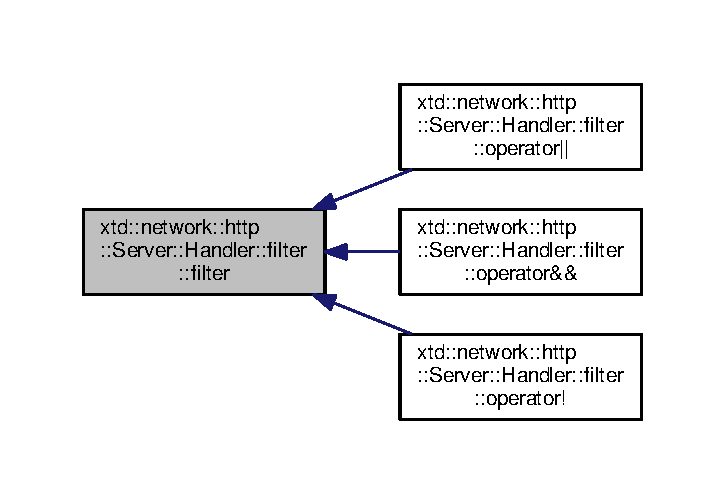
\includegraphics[width=348pt]{structxtd_1_1network_1_1http_1_1Server_1_1Handler_1_1filter_aade4e97fe12a8e43c647ac1ca7cc21c7_icgraph}
\end{center}
\end{figure}


\index{xtd\+::network\+::http\+::\+Server\+::\+Handler\+::filter@{xtd\+::network\+::http\+::\+Server\+::\+Handler\+::filter}!filter@{filter}}
\index{filter@{filter}!xtd\+::network\+::http\+::\+Server\+::\+Handler\+::filter@{xtd\+::network\+::http\+::\+Server\+::\+Handler\+::filter}}
\subsubsection[{\texorpdfstring{filter(\+A p\+\_\+method)}{filter(A p_method)}}]{\setlength{\rightskip}{0pt plus 5cm}template$<$typename Domain  = utils\+::af\+\_\+inet$>$ template$<$class A $>$ {\bf xtd\+::network\+::http\+::\+Server}$<$ Domain $>$\+::Handler\+::filter\+::filter (
\begin{DoxyParamCaption}
\item[{A}]{p\+\_\+method}
\end{DoxyParamCaption}
)\hspace{0.3cm}{\ttfamily [inline]}}\hypertarget{structxtd_1_1network_1_1http_1_1Server_1_1Handler_1_1filter_af56d192d61507e75ff21f4f075df1bd3}{}\label{structxtd_1_1network_1_1http_1_1Server_1_1Handler_1_1filter_af56d192d61507e75ff21f4f075df1bd3}


Definition at line 251 of file Server.\+hh.


\begin{DoxyCode}
251                          :
252         \hyperlink{structxtd_1_1network_1_1http_1_1Server_1_1Handler_1_1filter_a7a443c95291e03dff64632da70c3970e}{t\_func}(p\_method) \{ \}
\end{DoxyCode}
\index{xtd\+::network\+::http\+::\+Server\+::\+Handler\+::filter@{xtd\+::network\+::http\+::\+Server\+::\+Handler\+::filter}!filter@{filter}}
\index{filter@{filter}!xtd\+::network\+::http\+::\+Server\+::\+Handler\+::filter@{xtd\+::network\+::http\+::\+Server\+::\+Handler\+::filter}}
\subsubsection[{\texorpdfstring{filter(\+A p\+\_\+method, Base p\+\_\+instance)}{filter(A p_method, Base p_instance)}}]{\setlength{\rightskip}{0pt plus 5cm}template$<$typename Domain  = utils\+::af\+\_\+inet$>$ template$<$class A , typename Base $>$ {\bf xtd\+::network\+::http\+::\+Server}$<$ Domain $>$\+::Handler\+::filter\+::filter (
\begin{DoxyParamCaption}
\item[{A}]{p\+\_\+method, }
\item[{Base}]{p\+\_\+instance}
\end{DoxyParamCaption}
)\hspace{0.3cm}{\ttfamily [inline]}}\hypertarget{structxtd_1_1network_1_1http_1_1Server_1_1Handler_1_1filter_a47da45a50b8b22c1a141d1602ac9f9eb}{}\label{structxtd_1_1network_1_1http_1_1Server_1_1Handler_1_1filter_a47da45a50b8b22c1a141d1602ac9f9eb}


Definition at line 254 of file Server.\+hh.


\begin{DoxyCode}
254                                           :
255         \hyperlink{structxtd_1_1network_1_1http_1_1Server_1_1Handler_1_1filter_a7a443c95291e03dff64632da70c3970e}{t\_func}(boost::bind(p\_method, p\_instance, \_1)) \{ \}
\end{DoxyCode}
\index{xtd\+::network\+::http\+::\+Server\+::\+Handler\+::filter@{xtd\+::network\+::http\+::\+Server\+::\+Handler\+::filter}!filter@{filter}}
\index{filter@{filter}!xtd\+::network\+::http\+::\+Server\+::\+Handler\+::filter@{xtd\+::network\+::http\+::\+Server\+::\+Handler\+::filter}}
\subsubsection[{\texorpdfstring{filter(\+A p\+\_\+method, Base p\+\_\+instance, B p\+\_\+arg1)}{filter(A p_method, Base p_instance, B p_arg1)}}]{\setlength{\rightskip}{0pt plus 5cm}template$<$typename Domain  = utils\+::af\+\_\+inet$>$ template$<$class A , typename Base , typename B $>$ {\bf xtd\+::network\+::http\+::\+Server}$<$ Domain $>$\+::Handler\+::filter\+::filter (
\begin{DoxyParamCaption}
\item[{A}]{p\+\_\+method, }
\item[{Base}]{p\+\_\+instance, }
\item[{B}]{p\+\_\+arg1}
\end{DoxyParamCaption}
)\hspace{0.3cm}{\ttfamily [inline]}}\hypertarget{structxtd_1_1network_1_1http_1_1Server_1_1Handler_1_1filter_a4882bb6111bfa1007238091519723432}{}\label{structxtd_1_1network_1_1http_1_1Server_1_1Handler_1_1filter_a4882bb6111bfa1007238091519723432}


Definition at line 257 of file Server.\+hh.


\begin{DoxyCode}
257                                                     :
258         \hyperlink{structxtd_1_1network_1_1http_1_1Server_1_1Handler_1_1filter_a7a443c95291e03dff64632da70c3970e}{t\_func}(boost::bind(p\_method, p\_instance, p\_arg1, \_1)) \{ \}
\end{DoxyCode}
\index{xtd\+::network\+::http\+::\+Server\+::\+Handler\+::filter@{xtd\+::network\+::http\+::\+Server\+::\+Handler\+::filter}!filter@{filter}}
\index{filter@{filter}!xtd\+::network\+::http\+::\+Server\+::\+Handler\+::filter@{xtd\+::network\+::http\+::\+Server\+::\+Handler\+::filter}}
\subsubsection[{\texorpdfstring{filter(\+A p\+\_\+method, Base p\+\_\+instance, B p\+\_\+arg1, C p\+\_\+arg2)}{filter(A p_method, Base p_instance, B p_arg1, C p_arg2)}}]{\setlength{\rightskip}{0pt plus 5cm}template$<$typename Domain  = utils\+::af\+\_\+inet$>$ template$<$class A , typename Base , typename B , typename C $>$ {\bf xtd\+::network\+::http\+::\+Server}$<$ Domain $>$\+::Handler\+::filter\+::filter (
\begin{DoxyParamCaption}
\item[{A}]{p\+\_\+method, }
\item[{Base}]{p\+\_\+instance, }
\item[{B}]{p\+\_\+arg1, }
\item[{C}]{p\+\_\+arg2}
\end{DoxyParamCaption}
)\hspace{0.3cm}{\ttfamily [inline]}}\hypertarget{structxtd_1_1network_1_1http_1_1Server_1_1Handler_1_1filter_a9caa6426ff014b29d856845e542ecc61}{}\label{structxtd_1_1network_1_1http_1_1Server_1_1Handler_1_1filter_a9caa6426ff014b29d856845e542ecc61}


Definition at line 260 of file Server.\+hh.


\begin{DoxyCode}
260                                                               :
261         \hyperlink{structxtd_1_1network_1_1http_1_1Server_1_1Handler_1_1filter_a7a443c95291e03dff64632da70c3970e}{t\_func}(boost::bind(p\_method, p\_instance, p\_arg1, p\_arg2, \_1)) \{ \}
\end{DoxyCode}
\index{xtd\+::network\+::http\+::\+Server\+::\+Handler\+::filter@{xtd\+::network\+::http\+::\+Server\+::\+Handler\+::filter}!filter@{filter}}
\index{filter@{filter}!xtd\+::network\+::http\+::\+Server\+::\+Handler\+::filter@{xtd\+::network\+::http\+::\+Server\+::\+Handler\+::filter}}
\subsubsection[{\texorpdfstring{filter(\+A p\+\_\+method, Base p\+\_\+instance, B p\+\_\+arg1, C p\+\_\+arg2, D p\+\_\+arg3)}{filter(A p_method, Base p_instance, B p_arg1, C p_arg2, D p_arg3)}}]{\setlength{\rightskip}{0pt plus 5cm}template$<$typename Domain  = utils\+::af\+\_\+inet$>$ template$<$class A , typename Base , typename B , typename C , typename D $>$ {\bf xtd\+::network\+::http\+::\+Server}$<$ Domain $>$\+::Handler\+::filter\+::filter (
\begin{DoxyParamCaption}
\item[{A}]{p\+\_\+method, }
\item[{Base}]{p\+\_\+instance, }
\item[{B}]{p\+\_\+arg1, }
\item[{C}]{p\+\_\+arg2, }
\item[{D}]{p\+\_\+arg3}
\end{DoxyParamCaption}
)\hspace{0.3cm}{\ttfamily [inline]}}\hypertarget{structxtd_1_1network_1_1http_1_1Server_1_1Handler_1_1filter_aa73bc46ea27365b04dabc4ad3883f6e3}{}\label{structxtd_1_1network_1_1http_1_1Server_1_1Handler_1_1filter_aa73bc46ea27365b04dabc4ad3883f6e3}


Definition at line 263 of file Server.\+hh.


\begin{DoxyCode}
263                                                                         :
264         \hyperlink{structxtd_1_1network_1_1http_1_1Server_1_1Handler_1_1filter_a7a443c95291e03dff64632da70c3970e}{t\_func}(boost::bind(p\_method, p\_instance, p\_arg1, p\_arg2, p\_arg3, \_1)) \{ \}
\end{DoxyCode}


\subsection{Member Function Documentation}
\index{xtd\+::network\+::http\+::\+Server\+::\+Handler\+::filter@{xtd\+::network\+::http\+::\+Server\+::\+Handler\+::filter}!operator"!@{operator"!}}
\index{operator"!@{operator"!}!xtd\+::network\+::http\+::\+Server\+::\+Handler\+::filter@{xtd\+::network\+::http\+::\+Server\+::\+Handler\+::filter}}
\subsubsection[{\texorpdfstring{operator"!(void)}{operator!(void)}}]{\setlength{\rightskip}{0pt plus 5cm}template$<$typename Domain  = utils\+::af\+\_\+inet$>$ {\bf filter} {\bf xtd\+::network\+::http\+::\+Server}$<$ Domain $>$\+::Handler\+::filter\+::operator! (
\begin{DoxyParamCaption}
\item[{void}]{}
\end{DoxyParamCaption}
)\hspace{0.3cm}{\ttfamily [inline]}}\hypertarget{structxtd_1_1network_1_1http_1_1Server_1_1Handler_1_1filter_a86cabcb78e717225417801afb5ca0969}{}\label{structxtd_1_1network_1_1http_1_1Server_1_1Handler_1_1filter_a86cabcb78e717225417801afb5ca0969}


Definition at line 276 of file Server.\+hh.


\begin{DoxyCode}
277       \{
278         \textcolor{keywordflow}{return} \hyperlink{structxtd_1_1network_1_1http_1_1Server_1_1Handler_1_1filter_aade4e97fe12a8e43c647ac1ca7cc21c7}{filter}(!boost::bind(*\textcolor{keyword}{this}, \_1));
279       \}
\end{DoxyCode}


Here is the call graph for this function\+:
\nopagebreak
\begin{figure}[H]
\begin{center}
\leavevmode
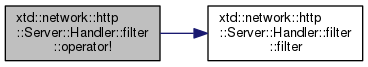
\includegraphics[width=348pt]{structxtd_1_1network_1_1http_1_1Server_1_1Handler_1_1filter_a86cabcb78e717225417801afb5ca0969_cgraph}
\end{center}
\end{figure}


\index{xtd\+::network\+::http\+::\+Server\+::\+Handler\+::filter@{xtd\+::network\+::http\+::\+Server\+::\+Handler\+::filter}!operator\&\&@{operator\&\&}}
\index{operator\&\&@{operator\&\&}!xtd\+::network\+::http\+::\+Server\+::\+Handler\+::filter@{xtd\+::network\+::http\+::\+Server\+::\+Handler\+::filter}}
\subsubsection[{\texorpdfstring{operator\&\&(filter p\+\_\+filter2)}{operator&&(filter p_filter2)}}]{\setlength{\rightskip}{0pt plus 5cm}template$<$typename Domain  = utils\+::af\+\_\+inet$>$ {\bf filter} {\bf xtd\+::network\+::http\+::\+Server}$<$ Domain $>$\+::Handler\+::filter\+::operator\&\& (
\begin{DoxyParamCaption}
\item[{{\bf filter}}]{p\+\_\+filter2}
\end{DoxyParamCaption}
)\hspace{0.3cm}{\ttfamily [inline]}}\hypertarget{structxtd_1_1network_1_1http_1_1Server_1_1Handler_1_1filter_a5da9bfbb2192792c99106f3969084395}{}\label{structxtd_1_1network_1_1http_1_1Server_1_1Handler_1_1filter_a5da9bfbb2192792c99106f3969084395}


Definition at line 271 of file Server.\+hh.


\begin{DoxyCode}
272       \{
273         \textcolor{keywordflow}{return} \hyperlink{structxtd_1_1network_1_1http_1_1Server_1_1Handler_1_1filter_aade4e97fe12a8e43c647ac1ca7cc21c7}{filter}(boost::bind(*\textcolor{keyword}{this},     \_1) &&
274                       boost::bind(p\_filter2, \_1));
275       \}
\end{DoxyCode}


Here is the call graph for this function\+:
\nopagebreak
\begin{figure}[H]
\begin{center}
\leavevmode
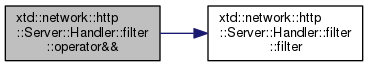
\includegraphics[width=348pt]{structxtd_1_1network_1_1http_1_1Server_1_1Handler_1_1filter_a5da9bfbb2192792c99106f3969084395_cgraph}
\end{center}
\end{figure}


\index{xtd\+::network\+::http\+::\+Server\+::\+Handler\+::filter@{xtd\+::network\+::http\+::\+Server\+::\+Handler\+::filter}!operator\texttt{"|}\texttt{"|}@{operator\texttt{"|}\texttt{"|}}}
\index{operator\texttt{"|}\texttt{"|}@{operator\texttt{"|}\texttt{"|}}!xtd\+::network\+::http\+::\+Server\+::\+Handler\+::filter@{xtd\+::network\+::http\+::\+Server\+::\+Handler\+::filter}}
\subsubsection[{\texorpdfstring{operator\texttt{"|}\texttt{"|}(filter p\+\_\+filter2)}{operator||(filter p_filter2)}}]{\setlength{\rightskip}{0pt plus 5cm}template$<$typename Domain  = utils\+::af\+\_\+inet$>$ {\bf filter} {\bf xtd\+::network\+::http\+::\+Server}$<$ Domain $>$\+::Handler\+::filter\+::operator$\vert$$\vert$ (
\begin{DoxyParamCaption}
\item[{{\bf filter}}]{p\+\_\+filter2}
\end{DoxyParamCaption}
)\hspace{0.3cm}{\ttfamily [inline]}}\hypertarget{structxtd_1_1network_1_1http_1_1Server_1_1Handler_1_1filter_a552b18f4f6e535a016d547ce0efc53c8}{}\label{structxtd_1_1network_1_1http_1_1Server_1_1Handler_1_1filter_a552b18f4f6e535a016d547ce0efc53c8}


Definition at line 266 of file Server.\+hh.


\begin{DoxyCode}
267       \{
268         \textcolor{keywordflow}{return} \hyperlink{structxtd_1_1network_1_1http_1_1Server_1_1Handler_1_1filter_aade4e97fe12a8e43c647ac1ca7cc21c7}{filter}(boost::bind(*\textcolor{keyword}{this},     \_1) ||
269                       boost::bind(p\_filter2, \_1));
270       \}
\end{DoxyCode}


Here is the call graph for this function\+:
\nopagebreak
\begin{figure}[H]
\begin{center}
\leavevmode
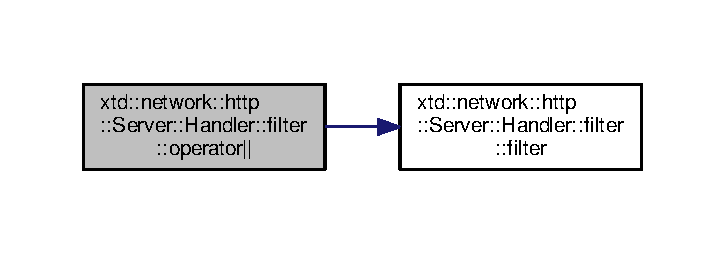
\includegraphics[width=348pt]{structxtd_1_1network_1_1http_1_1Server_1_1Handler_1_1filter_a552b18f4f6e535a016d547ce0efc53c8_cgraph}
\end{center}
\end{figure}




The documentation for this struct was generated from the following file\+:\begin{DoxyCompactItemize}
\item 
/home/psyco/dev/xtdcpp/network/src/http/\hyperlink{http_2Server_8hh}{Server.\+hh}\end{DoxyCompactItemize}

\hypertarget{classxtd_1_1network_1_1http_1_1Generator}{\section{xtd\-:\-:network\-:\-:http\-:\-:Generator Class Reference}
\label{classxtd_1_1network_1_1http_1_1Generator}\index{xtd\-::network\-::http\-::\-Generator@{xtd\-::network\-::http\-::\-Generator}}
}


{\ttfamily \#include $<$Template.\-hh$>$}



Inheritance diagram for xtd\-:\-:network\-:\-:http\-:\-:Generator\-:
\nopagebreak
\begin{figure}[H]
\begin{center}
\leavevmode
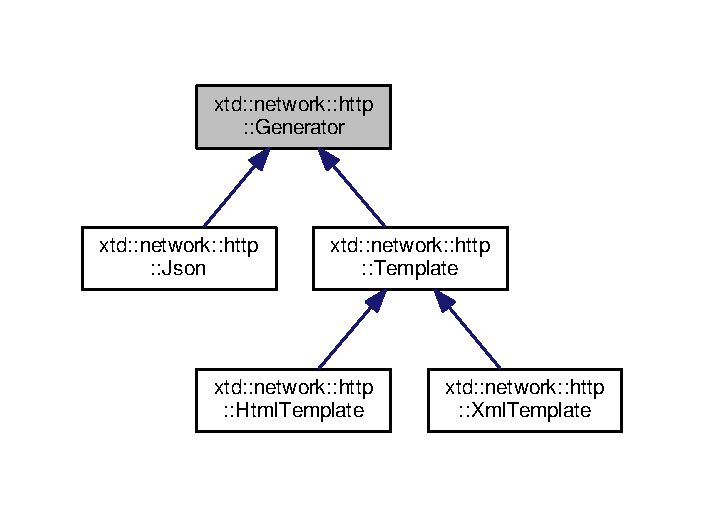
\includegraphics[width=338pt]{classxtd_1_1network_1_1http_1_1Generator__inherit__graph}
\end{center}
\end{figure}
\subsection*{Public Member Functions}
\begin{DoxyCompactItemize}
\item 
\hyperlink{classxtd_1_1network_1_1http_1_1Generator_a5f8bfffa6c7fe8ae46158e976af3d666}{Generator} (const string \&p\-\_\-content\-Type=\hyperlink{classxtd_1_1network_1_1http_1_1Generator_aef564fc3152e7477bb429e45b19328fc}{mcs\-\_\-default\-Content\-Type})
\item 
virtual \hyperlink{classxtd_1_1network_1_1http_1_1Generator_a1d1e0656a6ffeecd718230613681c56d}{$\sim$\-Generator} (void)
\item 
const string \& \hyperlink{classxtd_1_1network_1_1http_1_1Generator_a4052d01b0d4849321b61688eac757b41}{get\-Content\-Type} (void) const 
\item 
const string \& \hyperlink{classxtd_1_1network_1_1http_1_1Generator_ac4fa462833bedc8bde7c7e81b1a29f37}{get\-Error} (void) const 
\item 
virtual status \hyperlink{classxtd_1_1network_1_1http_1_1Generator_a20ee788dc76ee76f4be5f44091b655ca}{resolve} (string \&p\-\_\-result)=0
\end{DoxyCompactItemize}
\subsection*{Protected Member Functions}
\begin{DoxyCompactItemize}
\item 
void \hyperlink{classxtd_1_1network_1_1http_1_1Generator_a289cfd48cc9c5646c8f06455df41f09d}{add\-Error} (const string \&p\-\_\-error)
\end{DoxyCompactItemize}
\subsection*{Static Protected Attributes}
\begin{DoxyCompactItemize}
\item 
static const string \hyperlink{classxtd_1_1network_1_1http_1_1Generator_aef564fc3152e7477bb429e45b19328fc}{mcs\-\_\-default\-Content\-Type} = \char`\"{}text/plain\char`\"{}
\end{DoxyCompactItemize}


\subsection{Detailed Description}


Definition at line 13 of file Template.\-hh.



\subsection{Constructor \& Destructor Documentation}
\hypertarget{classxtd_1_1network_1_1http_1_1Generator_a5f8bfffa6c7fe8ae46158e976af3d666}{\index{xtd\-::network\-::http\-::\-Generator@{xtd\-::network\-::http\-::\-Generator}!Generator@{Generator}}
\index{Generator@{Generator}!xtd::network::http::Generator@{xtd\-::network\-::http\-::\-Generator}}
\subsubsection[{Generator}]{\setlength{\rightskip}{0pt plus 5cm}xtd\-::network\-::http\-::\-Generator\-::\-Generator (
\begin{DoxyParamCaption}
\item[{const string \&}]{p\-\_\-content\-Type = {\ttfamily {\bf mcs\-\_\-default\-Content\-Type}}}
\end{DoxyParamCaption}
)}}\label{classxtd_1_1network_1_1http_1_1Generator_a5f8bfffa6c7fe8ae46158e976af3d666}


Definition at line 55 of file Template.\-cc.


\begin{DoxyCode}
55                                                 :
56   m\_contentType(p\_contentType),
57   m\_error()
58 \{
59 \}
\end{DoxyCode}
\hypertarget{classxtd_1_1network_1_1http_1_1Generator_a1d1e0656a6ffeecd718230613681c56d}{\index{xtd\-::network\-::http\-::\-Generator@{xtd\-::network\-::http\-::\-Generator}!$\sim$\-Generator@{$\sim$\-Generator}}
\index{$\sim$\-Generator@{$\sim$\-Generator}!xtd::network::http::Generator@{xtd\-::network\-::http\-::\-Generator}}
\subsubsection[{$\sim$\-Generator}]{\setlength{\rightskip}{0pt plus 5cm}xtd\-::network\-::http\-::\-Generator\-::$\sim$\-Generator (
\begin{DoxyParamCaption}
\item[{void}]{}
\end{DoxyParamCaption}
)\hspace{0.3cm}{\ttfamily [virtual]}}}\label{classxtd_1_1network_1_1http_1_1Generator_a1d1e0656a6ffeecd718230613681c56d}


Definition at line 61 of file Template.\-cc.


\begin{DoxyCode}
62 \{
63 \}
\end{DoxyCode}


\subsection{Member Function Documentation}
\hypertarget{classxtd_1_1network_1_1http_1_1Generator_a289cfd48cc9c5646c8f06455df41f09d}{\index{xtd\-::network\-::http\-::\-Generator@{xtd\-::network\-::http\-::\-Generator}!add\-Error@{add\-Error}}
\index{add\-Error@{add\-Error}!xtd::network::http::Generator@{xtd\-::network\-::http\-::\-Generator}}
\subsubsection[{add\-Error}]{\setlength{\rightskip}{0pt plus 5cm}void xtd\-::network\-::http\-::\-Generator\-::add\-Error (
\begin{DoxyParamCaption}
\item[{const string \&}]{p\-\_\-error}
\end{DoxyParamCaption}
)\hspace{0.3cm}{\ttfamily [inline]}, {\ttfamily [protected]}}}\label{classxtd_1_1network_1_1http_1_1Generator_a289cfd48cc9c5646c8f06455df41f09d}


Here is the caller graph for this function\-:
\nopagebreak
\begin{figure}[H]
\begin{center}
\leavevmode
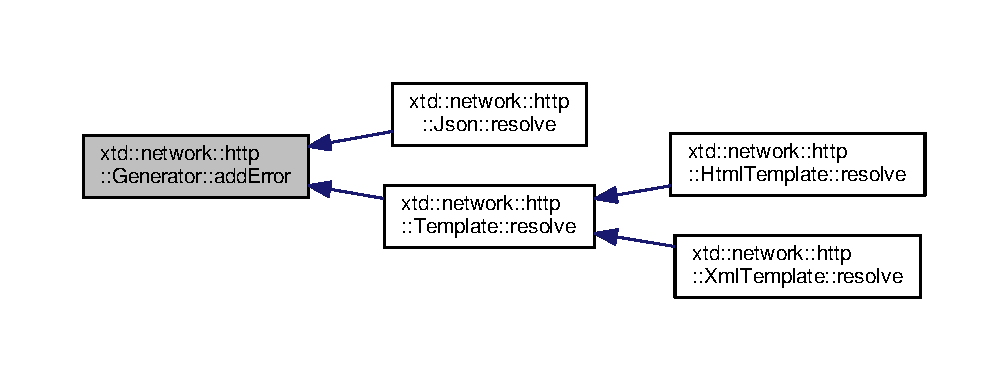
\includegraphics[width=350pt]{classxtd_1_1network_1_1http_1_1Generator_a289cfd48cc9c5646c8f06455df41f09d_icgraph}
\end{center}
\end{figure}


\hypertarget{classxtd_1_1network_1_1http_1_1Generator_a4052d01b0d4849321b61688eac757b41}{\index{xtd\-::network\-::http\-::\-Generator@{xtd\-::network\-::http\-::\-Generator}!get\-Content\-Type@{get\-Content\-Type}}
\index{get\-Content\-Type@{get\-Content\-Type}!xtd::network::http::Generator@{xtd\-::network\-::http\-::\-Generator}}
\subsubsection[{get\-Content\-Type}]{\setlength{\rightskip}{0pt plus 5cm}const string\& xtd\-::network\-::http\-::\-Generator\-::get\-Content\-Type (
\begin{DoxyParamCaption}
\item[{void}]{}
\end{DoxyParamCaption}
) const\hspace{0.3cm}{\ttfamily [inline]}}}\label{classxtd_1_1network_1_1http_1_1Generator_a4052d01b0d4849321b61688eac757b41}
\hypertarget{classxtd_1_1network_1_1http_1_1Generator_ac4fa462833bedc8bde7c7e81b1a29f37}{\index{xtd\-::network\-::http\-::\-Generator@{xtd\-::network\-::http\-::\-Generator}!get\-Error@{get\-Error}}
\index{get\-Error@{get\-Error}!xtd::network::http::Generator@{xtd\-::network\-::http\-::\-Generator}}
\subsubsection[{get\-Error}]{\setlength{\rightskip}{0pt plus 5cm}const string\& xtd\-::network\-::http\-::\-Generator\-::get\-Error (
\begin{DoxyParamCaption}
\item[{void}]{}
\end{DoxyParamCaption}
) const\hspace{0.3cm}{\ttfamily [inline]}}}\label{classxtd_1_1network_1_1http_1_1Generator_ac4fa462833bedc8bde7c7e81b1a29f37}
\hypertarget{classxtd_1_1network_1_1http_1_1Generator_a20ee788dc76ee76f4be5f44091b655ca}{\index{xtd\-::network\-::http\-::\-Generator@{xtd\-::network\-::http\-::\-Generator}!resolve@{resolve}}
\index{resolve@{resolve}!xtd::network::http::Generator@{xtd\-::network\-::http\-::\-Generator}}
\subsubsection[{resolve}]{\setlength{\rightskip}{0pt plus 5cm}virtual status xtd\-::network\-::http\-::\-Generator\-::resolve (
\begin{DoxyParamCaption}
\item[{string \&}]{p\-\_\-result}
\end{DoxyParamCaption}
)\hspace{0.3cm}{\ttfamily [pure virtual]}}}\label{classxtd_1_1network_1_1http_1_1Generator_a20ee788dc76ee76f4be5f44091b655ca}


Implemented in \hyperlink{classxtd_1_1network_1_1http_1_1XmlTemplate_ab221547a643e3db5ba99640fe14b9f68}{xtd\-::network\-::http\-::\-Xml\-Template}, \hyperlink{classxtd_1_1network_1_1http_1_1HtmlTemplate_af621b5bf866fa828f0bd5eaf225d5f70}{xtd\-::network\-::http\-::\-Html\-Template}, \hyperlink{classxtd_1_1network_1_1http_1_1Template_a476ce5e5b8465ea80ade07c003ab5cfd}{xtd\-::network\-::http\-::\-Template}, and \hyperlink{classxtd_1_1network_1_1http_1_1Json_a7a9ed4f957c77813ecbb84e228936b5e}{xtd\-::network\-::http\-::\-Json}.



\subsection{Member Data Documentation}
\hypertarget{classxtd_1_1network_1_1http_1_1Generator_aef564fc3152e7477bb429e45b19328fc}{\index{xtd\-::network\-::http\-::\-Generator@{xtd\-::network\-::http\-::\-Generator}!mcs\-\_\-default\-Content\-Type@{mcs\-\_\-default\-Content\-Type}}
\index{mcs\-\_\-default\-Content\-Type@{mcs\-\_\-default\-Content\-Type}!xtd::network::http::Generator@{xtd\-::network\-::http\-::\-Generator}}
\subsubsection[{mcs\-\_\-default\-Content\-Type}]{\setlength{\rightskip}{0pt plus 5cm}const string xtd\-::network\-::http\-::\-Generator\-::mcs\-\_\-default\-Content\-Type = \char`\"{}text/plain\char`\"{}\hspace{0.3cm}{\ttfamily [static]}, {\ttfamily [protected]}}}\label{classxtd_1_1network_1_1http_1_1Generator_aef564fc3152e7477bb429e45b19328fc}


Definition at line 16 of file Template.\-hh.



The documentation for this class was generated from the following files\-:\begin{DoxyCompactItemize}
\item 
/home/travis/build/psycofdj/xtdcpp/network/src/http/\hyperlink{Template_8hh}{Template.\-hh}\item 
/home/travis/build/psycofdj/xtdcpp/network/src/http/\hyperlink{Template_8cc}{Template.\-cc}\end{DoxyCompactItemize}

\hypertarget{classxtd_1_1network_1_1http_1_1Server_1_1Handler}{}\section{xtd\+:\+:network\+:\+:http\+:\+:Server$<$ Domain $>$\+:\+:Handler Class Reference}
\label{classxtd_1_1network_1_1http_1_1Server_1_1Handler}\index{xtd\+::network\+::http\+::\+Server$<$ Domain $>$\+::\+Handler@{xtd\+::network\+::http\+::\+Server$<$ Domain $>$\+::\+Handler}}


{\ttfamily \#include $<$Server.\+hh$>$}



Collaboration diagram for xtd\+:\+:network\+:\+:http\+:\+:Server$<$ Domain $>$\+:\+:Handler\+:
\nopagebreak
\begin{figure}[H]
\begin{center}
\leavevmode
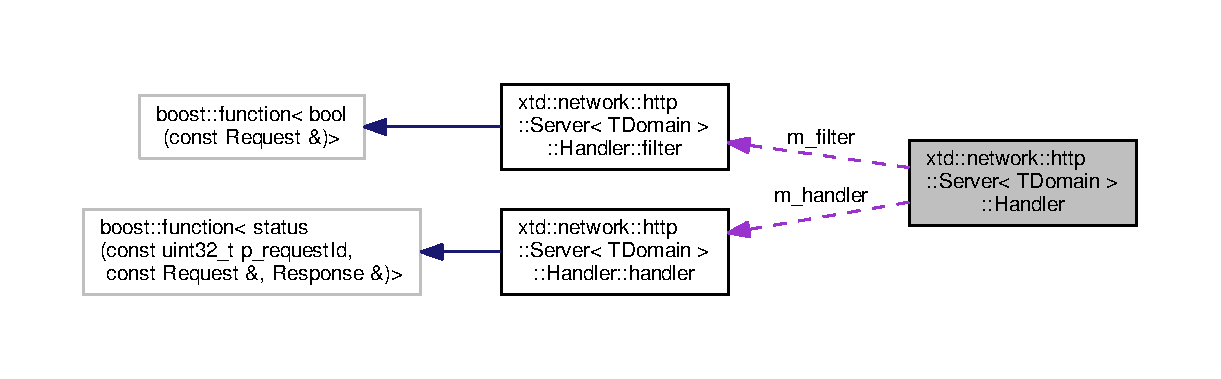
\includegraphics[width=350pt]{classxtd_1_1network_1_1http_1_1Server_1_1Handler__coll__graph}
\end{center}
\end{figure}
\subsection*{Classes}
\begin{DoxyCompactItemize}
\item 
struct \hyperlink{structxtd_1_1network_1_1http_1_1Server_1_1Handler_1_1filter}{filter}
\item 
struct \hyperlink{structxtd_1_1network_1_1http_1_1Server_1_1Handler_1_1handler}{handler}
\end{DoxyCompactItemize}
\subsection*{Public Types}
\begin{DoxyCompactItemize}
\item 
typedef vector$<$ \hyperlink{classxtd_1_1network_1_1http_1_1Server_1_1Handler}{Handler} $>$ \hyperlink{classxtd_1_1network_1_1http_1_1Server_1_1Handler_a840883d08fcdd990dbe33b660ee6febb}{t\+\_\+listof}
\end{DoxyCompactItemize}
\subsection*{Public Member Functions}
\begin{DoxyCompactItemize}
\item 
\hyperlink{classxtd_1_1network_1_1http_1_1Server_1_1Handler_a509777bdc769cabb23f04728e745b823}{Handler} (void)
\end{DoxyCompactItemize}
\subsection*{Static Public Member Functions}
\begin{DoxyCompactItemize}
\item 
static bool \hyperlink{classxtd_1_1network_1_1http_1_1Server_1_1Handler_a91c38afd6870731fe9f1b79d2cfda19f}{less} (const \hyperlink{classxtd_1_1network_1_1http_1_1Server_1_1Handler}{Handler} \&p\+\_\+obj1, const \hyperlink{classxtd_1_1network_1_1http_1_1Server_1_1Handler}{Handler} \&p\+\_\+obj2)
\end{DoxyCompactItemize}
\subsection*{Public Attributes}
\begin{DoxyCompactItemize}
\item 
string \hyperlink{classxtd_1_1network_1_1http_1_1Server_1_1Handler_aaea3487ea9687e61c40453d90841b223}{m\+\_\+path}
\item 
\hyperlink{structxtd_1_1network_1_1http_1_1Server_1_1Handler_1_1handler}{handler} \hyperlink{classxtd_1_1network_1_1http_1_1Server_1_1Handler_a4dfed2def9b251595d4ee176c106882f}{m\+\_\+handler}
\item 
\hyperlink{structxtd_1_1network_1_1http_1_1Server_1_1Handler_1_1filter}{filter} \hyperlink{classxtd_1_1network_1_1http_1_1Server_1_1Handler_a95854563aaa6e9c7fcced63d351e47a3}{m\+\_\+filter}
\item 
bool \hyperlink{classxtd_1_1network_1_1http_1_1Server_1_1Handler_a7605921b1ffffb66376920cfa6ebcb08}{m\+\_\+match\+Any}
\item 
string \hyperlink{classxtd_1_1network_1_1http_1_1Server_1_1Handler_aae46aaaf81c803b4ac6dd1a5b60feb36}{m\+\_\+descr}
\end{DoxyCompactItemize}


\subsection{Detailed Description}
\subsubsection*{template$<$typename Domain = utils\+::af\+\_\+inet$>$\\*
class xtd\+::network\+::http\+::\+Server$<$ Domain $>$\+::\+Handler}



Definition at line 238 of file Server.\+hh.



\subsection{Member Typedef Documentation}
\index{xtd\+::network\+::http\+::\+Server\+::\+Handler@{xtd\+::network\+::http\+::\+Server\+::\+Handler}!t\+\_\+listof@{t\+\_\+listof}}
\index{t\+\_\+listof@{t\+\_\+listof}!xtd\+::network\+::http\+::\+Server\+::\+Handler@{xtd\+::network\+::http\+::\+Server\+::\+Handler}}
\subsubsection[{\texorpdfstring{t\+\_\+listof}{t_listof}}]{\setlength{\rightskip}{0pt plus 5cm}template$<$typename Domain  = utils\+::af\+\_\+inet$>$ typedef vector$<${\bf Handler}$>$ {\bf xtd\+::network\+::http\+::\+Server}$<$ Domain $>$\+::{\bf Handler\+::t\+\_\+listof}}\hypertarget{classxtd_1_1network_1_1http_1_1Server_1_1Handler_a840883d08fcdd990dbe33b660ee6febb}{}\label{classxtd_1_1network_1_1http_1_1Server_1_1Handler_a840883d08fcdd990dbe33b660ee6febb}


Definition at line 241 of file Server.\+hh.



\subsection{Constructor \& Destructor Documentation}
\index{xtd\+::network\+::http\+::\+Server\+::\+Handler@{xtd\+::network\+::http\+::\+Server\+::\+Handler}!Handler@{Handler}}
\index{Handler@{Handler}!xtd\+::network\+::http\+::\+Server\+::\+Handler@{xtd\+::network\+::http\+::\+Server\+::\+Handler}}
\subsubsection[{\texorpdfstring{Handler(void)}{Handler(void)}}]{\setlength{\rightskip}{0pt plus 5cm}template$<$typename Domain  = utils\+::af\+\_\+inet$>$ {\bf xtd\+::network\+::http\+::\+Server}$<$ Domain $>$\+::Handler\+::\+Handler (
\begin{DoxyParamCaption}
\item[{void}]{}
\end{DoxyParamCaption}
)}\hypertarget{classxtd_1_1network_1_1http_1_1Server_1_1Handler_a509777bdc769cabb23f04728e745b823}{}\label{classxtd_1_1network_1_1http_1_1Server_1_1Handler_a509777bdc769cabb23f04728e745b823}


Here is the caller graph for this function\+:
\nopagebreak
\begin{figure}[H]
\begin{center}
\leavevmode
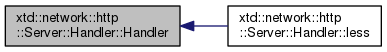
\includegraphics[width=350pt]{classxtd_1_1network_1_1http_1_1Server_1_1Handler_a509777bdc769cabb23f04728e745b823_icgraph}
\end{center}
\end{figure}




\subsection{Member Function Documentation}
\index{xtd\+::network\+::http\+::\+Server\+::\+Handler@{xtd\+::network\+::http\+::\+Server\+::\+Handler}!less@{less}}
\index{less@{less}!xtd\+::network\+::http\+::\+Server\+::\+Handler@{xtd\+::network\+::http\+::\+Server\+::\+Handler}}
\subsubsection[{\texorpdfstring{less(const Handler \&p\+\_\+obj1, const Handler \&p\+\_\+obj2)}{less(const Handler &p_obj1, const Handler &p_obj2)}}]{\setlength{\rightskip}{0pt plus 5cm}template$<$typename Domain  = utils\+::af\+\_\+inet$>$ static bool {\bf xtd\+::network\+::http\+::\+Server}$<$ Domain $>$\+::Handler\+::less (
\begin{DoxyParamCaption}
\item[{const {\bf Handler} \&}]{p\+\_\+obj1, }
\item[{const {\bf Handler} \&}]{p\+\_\+obj2}
\end{DoxyParamCaption}
)\hspace{0.3cm}{\ttfamily [inline]}, {\ttfamily [static]}}\hypertarget{classxtd_1_1network_1_1http_1_1Server_1_1Handler_a91c38afd6870731fe9f1b79d2cfda19f}{}\label{classxtd_1_1network_1_1http_1_1Server_1_1Handler_a91c38afd6870731fe9f1b79d2cfda19f}


Definition at line 303 of file Server.\+hh.


\begin{DoxyCode}
304     \{
305       \textcolor{keywordflow}{if} (p\_obj1.m\_matchAny == p\_obj2.m\_matchAny)
306         \textcolor{keywordflow}{return} std::less<string>()(p\_obj2.m\_path, p\_obj1.m\_path);
307       \textcolor{keywordflow}{return} std::less<bool>()(p\_obj1.m\_matchAny, p\_obj2.m\_matchAny);
308     \}
\end{DoxyCode}


Here is the call graph for this function\+:
\nopagebreak
\begin{figure}[H]
\begin{center}
\leavevmode
\includegraphics[width=350pt]{classxtd_1_1network_1_1http_1_1Server_1_1Handler_a91c38afd6870731fe9f1b79d2cfda19f_cgraph}
\end{center}
\end{figure}




\subsection{Member Data Documentation}
\index{xtd\+::network\+::http\+::\+Server\+::\+Handler@{xtd\+::network\+::http\+::\+Server\+::\+Handler}!m\+\_\+descr@{m\+\_\+descr}}
\index{m\+\_\+descr@{m\+\_\+descr}!xtd\+::network\+::http\+::\+Server\+::\+Handler@{xtd\+::network\+::http\+::\+Server\+::\+Handler}}
\subsubsection[{\texorpdfstring{m\+\_\+descr}{m_descr}}]{\setlength{\rightskip}{0pt plus 5cm}template$<$typename Domain  = utils\+::af\+\_\+inet$>$ string {\bf xtd\+::network\+::http\+::\+Server}$<$ Domain $>$\+::Handler\+::m\+\_\+descr}\hypertarget{classxtd_1_1network_1_1http_1_1Server_1_1Handler_aae46aaaf81c803b4ac6dd1a5b60feb36}{}\label{classxtd_1_1network_1_1http_1_1Server_1_1Handler_aae46aaaf81c803b4ac6dd1a5b60feb36}


Definition at line 317 of file Server.\+hh.

\index{xtd\+::network\+::http\+::\+Server\+::\+Handler@{xtd\+::network\+::http\+::\+Server\+::\+Handler}!m\+\_\+filter@{m\+\_\+filter}}
\index{m\+\_\+filter@{m\+\_\+filter}!xtd\+::network\+::http\+::\+Server\+::\+Handler@{xtd\+::network\+::http\+::\+Server\+::\+Handler}}
\subsubsection[{\texorpdfstring{m\+\_\+filter}{m_filter}}]{\setlength{\rightskip}{0pt plus 5cm}template$<$typename Domain  = utils\+::af\+\_\+inet$>$ {\bf filter} {\bf xtd\+::network\+::http\+::\+Server}$<$ Domain $>$\+::Handler\+::m\+\_\+filter}\hypertarget{classxtd_1_1network_1_1http_1_1Server_1_1Handler_a95854563aaa6e9c7fcced63d351e47a3}{}\label{classxtd_1_1network_1_1http_1_1Server_1_1Handler_a95854563aaa6e9c7fcced63d351e47a3}


Definition at line 315 of file Server.\+hh.

\index{xtd\+::network\+::http\+::\+Server\+::\+Handler@{xtd\+::network\+::http\+::\+Server\+::\+Handler}!m\+\_\+handler@{m\+\_\+handler}}
\index{m\+\_\+handler@{m\+\_\+handler}!xtd\+::network\+::http\+::\+Server\+::\+Handler@{xtd\+::network\+::http\+::\+Server\+::\+Handler}}
\subsubsection[{\texorpdfstring{m\+\_\+handler}{m_handler}}]{\setlength{\rightskip}{0pt plus 5cm}template$<$typename Domain  = utils\+::af\+\_\+inet$>$ {\bf handler} {\bf xtd\+::network\+::http\+::\+Server}$<$ Domain $>$\+::Handler\+::m\+\_\+handler}\hypertarget{classxtd_1_1network_1_1http_1_1Server_1_1Handler_a4dfed2def9b251595d4ee176c106882f}{}\label{classxtd_1_1network_1_1http_1_1Server_1_1Handler_a4dfed2def9b251595d4ee176c106882f}


Definition at line 314 of file Server.\+hh.

\index{xtd\+::network\+::http\+::\+Server\+::\+Handler@{xtd\+::network\+::http\+::\+Server\+::\+Handler}!m\+\_\+match\+Any@{m\+\_\+match\+Any}}
\index{m\+\_\+match\+Any@{m\+\_\+match\+Any}!xtd\+::network\+::http\+::\+Server\+::\+Handler@{xtd\+::network\+::http\+::\+Server\+::\+Handler}}
\subsubsection[{\texorpdfstring{m\+\_\+match\+Any}{m_matchAny}}]{\setlength{\rightskip}{0pt plus 5cm}template$<$typename Domain  = utils\+::af\+\_\+inet$>$ bool {\bf xtd\+::network\+::http\+::\+Server}$<$ Domain $>$\+::Handler\+::m\+\_\+match\+Any}\hypertarget{classxtd_1_1network_1_1http_1_1Server_1_1Handler_a7605921b1ffffb66376920cfa6ebcb08}{}\label{classxtd_1_1network_1_1http_1_1Server_1_1Handler_a7605921b1ffffb66376920cfa6ebcb08}


Definition at line 316 of file Server.\+hh.

\index{xtd\+::network\+::http\+::\+Server\+::\+Handler@{xtd\+::network\+::http\+::\+Server\+::\+Handler}!m\+\_\+path@{m\+\_\+path}}
\index{m\+\_\+path@{m\+\_\+path}!xtd\+::network\+::http\+::\+Server\+::\+Handler@{xtd\+::network\+::http\+::\+Server\+::\+Handler}}
\subsubsection[{\texorpdfstring{m\+\_\+path}{m_path}}]{\setlength{\rightskip}{0pt plus 5cm}template$<$typename Domain  = utils\+::af\+\_\+inet$>$ string {\bf xtd\+::network\+::http\+::\+Server}$<$ Domain $>$\+::Handler\+::m\+\_\+path}\hypertarget{classxtd_1_1network_1_1http_1_1Server_1_1Handler_aaea3487ea9687e61c40453d90841b223}{}\label{classxtd_1_1network_1_1http_1_1Server_1_1Handler_aaea3487ea9687e61c40453d90841b223}


Definition at line 313 of file Server.\+hh.



The documentation for this class was generated from the following file\+:\begin{DoxyCompactItemize}
\item 
/home/psyco/dev/xtdcpp/network/src/http/\hyperlink{http_2Server_8hh}{Server.\+hh}\end{DoxyCompactItemize}

\hypertarget{structxtd_1_1network_1_1http_1_1Server_1_1Handler_1_1handler}{}\section{xtd\+:\+:network\+:\+:http\+:\+:Server$<$ Domain $>$\+:\+:Handler\+:\+:handler Struct Reference}
\label{structxtd_1_1network_1_1http_1_1Server_1_1Handler_1_1handler}\index{xtd\+::network\+::http\+::\+Server$<$ Domain $>$\+::\+Handler\+::handler@{xtd\+::network\+::http\+::\+Server$<$ Domain $>$\+::\+Handler\+::handler}}


{\ttfamily \#include $<$Server.\+hh$>$}



Inheritance diagram for xtd\+:\+:network\+:\+:http\+:\+:Server$<$ Domain $>$\+:\+:Handler\+:\+:handler\+:
\nopagebreak
\begin{figure}[H]
\begin{center}
\leavevmode
\includegraphics[width=350pt]{structxtd_1_1network_1_1http_1_1Server_1_1Handler_1_1handler__inherit__graph}
\end{center}
\end{figure}


Collaboration diagram for xtd\+:\+:network\+:\+:http\+:\+:Server$<$ Domain $>$\+:\+:Handler\+:\+:handler\+:
\nopagebreak
\begin{figure}[H]
\begin{center}
\leavevmode
\includegraphics[width=350pt]{structxtd_1_1network_1_1http_1_1Server_1_1Handler_1_1handler__coll__graph}
\end{center}
\end{figure}
\subsection*{Public Types}
\begin{DoxyCompactItemize}
\item 
typedef boost\+::function$<$ status(const uint32\+\_\+t p\+\_\+request\+Id, const \hyperlink{classxtd_1_1network_1_1http_1_1Request}{Request} \&, \hyperlink{classxtd_1_1network_1_1http_1_1Response}{Response} \&)$>$ \hyperlink{structxtd_1_1network_1_1http_1_1Server_1_1Handler_1_1handler_acd37ef7fd8a395e1bfa372ad3c025253}{t\+\_\+func}
\end{DoxyCompactItemize}
\subsection*{Public Member Functions}
\begin{DoxyCompactItemize}
\item 
\hyperlink{structxtd_1_1network_1_1http_1_1Server_1_1Handler_1_1handler_a590cb56ee70081b73e98b47c0d50b3f1}{handler} (void)
\item 
{\footnotesize template$<$class A , typename Base $>$ }\\\hyperlink{structxtd_1_1network_1_1http_1_1Server_1_1Handler_1_1handler_a8fe309868dbefb2fbbdda593782728f6}{handler} (A p\+\_\+method, Base p\+\_\+instance)
\item 
{\footnotesize template$<$class A , typename Base , typename B $>$ }\\\hyperlink{structxtd_1_1network_1_1http_1_1Server_1_1Handler_1_1handler_ab6f310afe2dcb6c474906f42986bce4d}{handler} (A p\+\_\+method, Base p\+\_\+instance, B p\+\_\+arg1)
\item 
{\footnotesize template$<$class A , typename Base , typename B , typename C $>$ }\\\hyperlink{structxtd_1_1network_1_1http_1_1Server_1_1Handler_1_1handler_a64993bf20fa797e2e174adeb0bcd520d}{handler} (A p\+\_\+method, Base p\+\_\+instance, B p\+\_\+arg1, C p\+\_\+arg2)
\item 
{\footnotesize template$<$class A , typename Base , typename B , typename C , typename D $>$ }\\\hyperlink{structxtd_1_1network_1_1http_1_1Server_1_1Handler_1_1handler_af7e711a4e11ebc9fb1c5399f030ce778}{handler} (A p\+\_\+method, Base p\+\_\+instance, B p\+\_\+arg1, C p\+\_\+arg2, D p\+\_\+arg3)
\end{DoxyCompactItemize}


\subsection{Detailed Description}
\subsubsection*{template$<$typename Domain = utils\+::af\+\_\+inet$>$\\*
struct xtd\+::network\+::http\+::\+Server$<$ Domain $>$\+::\+Handler\+::handler}



Definition at line 282 of file Server.\+hh.



\subsection{Member Typedef Documentation}
\index{xtd\+::network\+::http\+::\+Server\+::\+Handler\+::handler@{xtd\+::network\+::http\+::\+Server\+::\+Handler\+::handler}!t\+\_\+func@{t\+\_\+func}}
\index{t\+\_\+func@{t\+\_\+func}!xtd\+::network\+::http\+::\+Server\+::\+Handler\+::handler@{xtd\+::network\+::http\+::\+Server\+::\+Handler\+::handler}}
\subsubsection[{\texorpdfstring{t\+\_\+func}{t_func}}]{\setlength{\rightskip}{0pt plus 5cm}template$<$typename Domain  = utils\+::af\+\_\+inet$>$ typedef boost\+::function$<$status (const uint32\+\_\+t p\+\_\+request\+Id, const {\bf Request}\&, {\bf Response}\&)$>$ {\bf xtd\+::network\+::http\+::\+Server}$<$ Domain $>$\+::{\bf Handler\+::handler\+::t\+\_\+func}}\hypertarget{structxtd_1_1network_1_1http_1_1Server_1_1Handler_1_1handler_acd37ef7fd8a395e1bfa372ad3c025253}{}\label{structxtd_1_1network_1_1http_1_1Server_1_1Handler_1_1handler_acd37ef7fd8a395e1bfa372ad3c025253}


Definition at line 285 of file Server.\+hh.



\subsection{Constructor \& Destructor Documentation}
\index{xtd\+::network\+::http\+::\+Server\+::\+Handler\+::handler@{xtd\+::network\+::http\+::\+Server\+::\+Handler\+::handler}!handler@{handler}}
\index{handler@{handler}!xtd\+::network\+::http\+::\+Server\+::\+Handler\+::handler@{xtd\+::network\+::http\+::\+Server\+::\+Handler\+::handler}}
\subsubsection[{\texorpdfstring{handler(void)}{handler(void)}}]{\setlength{\rightskip}{0pt plus 5cm}template$<$typename Domain  = utils\+::af\+\_\+inet$>$ {\bf xtd\+::network\+::http\+::\+Server}$<$ Domain $>$\+::Handler\+::handler\+::handler (
\begin{DoxyParamCaption}
\item[{void}]{}
\end{DoxyParamCaption}
)\hspace{0.3cm}{\ttfamily [inline]}}\hypertarget{structxtd_1_1network_1_1http_1_1Server_1_1Handler_1_1handler_a590cb56ee70081b73e98b47c0d50b3f1}{}\label{structxtd_1_1network_1_1http_1_1Server_1_1Handler_1_1handler_a590cb56ee70081b73e98b47c0d50b3f1}


Definition at line 287 of file Server.\+hh.


\begin{DoxyCode}
287                     :
288         \hyperlink{structxtd_1_1network_1_1http_1_1Server_1_1Handler_1_1handler_acd37ef7fd8a395e1bfa372ad3c025253}{t\_func}() \{ \}
\end{DoxyCode}
\index{xtd\+::network\+::http\+::\+Server\+::\+Handler\+::handler@{xtd\+::network\+::http\+::\+Server\+::\+Handler\+::handler}!handler@{handler}}
\index{handler@{handler}!xtd\+::network\+::http\+::\+Server\+::\+Handler\+::handler@{xtd\+::network\+::http\+::\+Server\+::\+Handler\+::handler}}
\subsubsection[{\texorpdfstring{handler(\+A p\+\_\+method, Base p\+\_\+instance)}{handler(A p_method, Base p_instance)}}]{\setlength{\rightskip}{0pt plus 5cm}template$<$typename Domain  = utils\+::af\+\_\+inet$>$ template$<$class A , typename Base $>$ {\bf xtd\+::network\+::http\+::\+Server}$<$ Domain $>$\+::Handler\+::handler\+::handler (
\begin{DoxyParamCaption}
\item[{A}]{p\+\_\+method, }
\item[{Base}]{p\+\_\+instance}
\end{DoxyParamCaption}
)\hspace{0.3cm}{\ttfamily [inline]}}\hypertarget{structxtd_1_1network_1_1http_1_1Server_1_1Handler_1_1handler_a8fe309868dbefb2fbbdda593782728f6}{}\label{structxtd_1_1network_1_1http_1_1Server_1_1Handler_1_1handler_a8fe309868dbefb2fbbdda593782728f6}


Definition at line 290 of file Server.\+hh.


\begin{DoxyCode}
290                                            :
291         \hyperlink{structxtd_1_1network_1_1http_1_1Server_1_1Handler_1_1handler_acd37ef7fd8a395e1bfa372ad3c025253}{t\_func}(boost::bind(p\_method, p\_instance, \_1, \_2, \_3)) \{ \}
\end{DoxyCode}
\index{xtd\+::network\+::http\+::\+Server\+::\+Handler\+::handler@{xtd\+::network\+::http\+::\+Server\+::\+Handler\+::handler}!handler@{handler}}
\index{handler@{handler}!xtd\+::network\+::http\+::\+Server\+::\+Handler\+::handler@{xtd\+::network\+::http\+::\+Server\+::\+Handler\+::handler}}
\subsubsection[{\texorpdfstring{handler(\+A p\+\_\+method, Base p\+\_\+instance, B p\+\_\+arg1)}{handler(A p_method, Base p_instance, B p_arg1)}}]{\setlength{\rightskip}{0pt plus 5cm}template$<$typename Domain  = utils\+::af\+\_\+inet$>$ template$<$class A , typename Base , typename B $>$ {\bf xtd\+::network\+::http\+::\+Server}$<$ Domain $>$\+::Handler\+::handler\+::handler (
\begin{DoxyParamCaption}
\item[{A}]{p\+\_\+method, }
\item[{Base}]{p\+\_\+instance, }
\item[{B}]{p\+\_\+arg1}
\end{DoxyParamCaption}
)\hspace{0.3cm}{\ttfamily [inline]}}\hypertarget{structxtd_1_1network_1_1http_1_1Server_1_1Handler_1_1handler_ab6f310afe2dcb6c474906f42986bce4d}{}\label{structxtd_1_1network_1_1http_1_1Server_1_1Handler_1_1handler_ab6f310afe2dcb6c474906f42986bce4d}


Definition at line 293 of file Server.\+hh.


\begin{DoxyCode}
293                                                      :
294         \hyperlink{structxtd_1_1network_1_1http_1_1Server_1_1Handler_1_1handler_acd37ef7fd8a395e1bfa372ad3c025253}{t\_func}(boost::bind(p\_method, p\_instance, p\_arg1, \_1, \_2, \_3)) \{ \}
\end{DoxyCode}
\index{xtd\+::network\+::http\+::\+Server\+::\+Handler\+::handler@{xtd\+::network\+::http\+::\+Server\+::\+Handler\+::handler}!handler@{handler}}
\index{handler@{handler}!xtd\+::network\+::http\+::\+Server\+::\+Handler\+::handler@{xtd\+::network\+::http\+::\+Server\+::\+Handler\+::handler}}
\subsubsection[{\texorpdfstring{handler(\+A p\+\_\+method, Base p\+\_\+instance, B p\+\_\+arg1, C p\+\_\+arg2)}{handler(A p_method, Base p_instance, B p_arg1, C p_arg2)}}]{\setlength{\rightskip}{0pt plus 5cm}template$<$typename Domain  = utils\+::af\+\_\+inet$>$ template$<$class A , typename Base , typename B , typename C $>$ {\bf xtd\+::network\+::http\+::\+Server}$<$ Domain $>$\+::Handler\+::handler\+::handler (
\begin{DoxyParamCaption}
\item[{A}]{p\+\_\+method, }
\item[{Base}]{p\+\_\+instance, }
\item[{B}]{p\+\_\+arg1, }
\item[{C}]{p\+\_\+arg2}
\end{DoxyParamCaption}
)\hspace{0.3cm}{\ttfamily [inline]}}\hypertarget{structxtd_1_1network_1_1http_1_1Server_1_1Handler_1_1handler_a64993bf20fa797e2e174adeb0bcd520d}{}\label{structxtd_1_1network_1_1http_1_1Server_1_1Handler_1_1handler_a64993bf20fa797e2e174adeb0bcd520d}


Definition at line 296 of file Server.\+hh.


\begin{DoxyCode}
296                                                                :
297         \hyperlink{structxtd_1_1network_1_1http_1_1Server_1_1Handler_1_1handler_acd37ef7fd8a395e1bfa372ad3c025253}{t\_func}(boost::bind(p\_method, p\_instance, p\_arg1, p\_arg2, \_1, \_2, \_3)) \{ \}
\end{DoxyCode}
\index{xtd\+::network\+::http\+::\+Server\+::\+Handler\+::handler@{xtd\+::network\+::http\+::\+Server\+::\+Handler\+::handler}!handler@{handler}}
\index{handler@{handler}!xtd\+::network\+::http\+::\+Server\+::\+Handler\+::handler@{xtd\+::network\+::http\+::\+Server\+::\+Handler\+::handler}}
\subsubsection[{\texorpdfstring{handler(\+A p\+\_\+method, Base p\+\_\+instance, B p\+\_\+arg1, C p\+\_\+arg2, D p\+\_\+arg3)}{handler(A p_method, Base p_instance, B p_arg1, C p_arg2, D p_arg3)}}]{\setlength{\rightskip}{0pt plus 5cm}template$<$typename Domain  = utils\+::af\+\_\+inet$>$ template$<$class A , typename Base , typename B , typename C , typename D $>$ {\bf xtd\+::network\+::http\+::\+Server}$<$ Domain $>$\+::Handler\+::handler\+::handler (
\begin{DoxyParamCaption}
\item[{A}]{p\+\_\+method, }
\item[{Base}]{p\+\_\+instance, }
\item[{B}]{p\+\_\+arg1, }
\item[{C}]{p\+\_\+arg2, }
\item[{D}]{p\+\_\+arg3}
\end{DoxyParamCaption}
)\hspace{0.3cm}{\ttfamily [inline]}}\hypertarget{structxtd_1_1network_1_1http_1_1Server_1_1Handler_1_1handler_af7e711a4e11ebc9fb1c5399f030ce778}{}\label{structxtd_1_1network_1_1http_1_1Server_1_1Handler_1_1handler_af7e711a4e11ebc9fb1c5399f030ce778}


Definition at line 299 of file Server.\+hh.


\begin{DoxyCode}
299                                                                          :
300         \hyperlink{structxtd_1_1network_1_1http_1_1Server_1_1Handler_1_1handler_acd37ef7fd8a395e1bfa372ad3c025253}{t\_func}(boost::bind(p\_method, p\_instance, p\_arg1, p\_arg2, p\_arg3, \_1, \_2, \_3)) \{ \}
\end{DoxyCode}


The documentation for this struct was generated from the following file\+:\begin{DoxyCompactItemize}
\item 
/home/psyco/dev/xtdcpp/network/src/http/\hyperlink{http_2Server_8hh}{Server.\+hh}\end{DoxyCompactItemize}

\hypertarget{structxtd_1_1network_1_1http_1_1hex__to__string}{}\section{xtd\+:\+:network\+:\+:http\+:\+:hex\+\_\+to\+\_\+string Struct Reference}
\label{structxtd_1_1network_1_1http_1_1hex__to__string}\index{xtd\+::network\+::http\+::hex\+\_\+to\+\_\+string@{xtd\+::network\+::http\+::hex\+\_\+to\+\_\+string}}
\subsection*{Public Member Functions}
\begin{DoxyCompactItemize}
\item 
{\footnotesize template$<$typename T $>$ }\\string \hyperlink{structxtd_1_1network_1_1http_1_1hex__to__string_a88d313368d68cfdddb20e4496b73af87}{operator()} (const T \&p\+\_\+match) const 
\end{DoxyCompactItemize}


\subsection{Detailed Description}


Definition at line 341 of file Request.\+cc.



\subsection{Member Function Documentation}
\index{xtd\+::network\+::http\+::hex\+\_\+to\+\_\+string@{xtd\+::network\+::http\+::hex\+\_\+to\+\_\+string}!operator()@{operator()}}
\index{operator()@{operator()}!xtd\+::network\+::http\+::hex\+\_\+to\+\_\+string@{xtd\+::network\+::http\+::hex\+\_\+to\+\_\+string}}
\subsubsection[{\texorpdfstring{operator()(const T \&p\+\_\+match) const }{operator()(const T &p_match) const }}]{\setlength{\rightskip}{0pt plus 5cm}template$<$typename T $>$ string xtd\+::network\+::http\+::hex\+\_\+to\+\_\+string\+::operator() (
\begin{DoxyParamCaption}
\item[{const T \&}]{p\+\_\+match}
\end{DoxyParamCaption}
) const\hspace{0.3cm}{\ttfamily [inline]}}\hypertarget{structxtd_1_1network_1_1http_1_1hex__to__string_a88d313368d68cfdddb20e4496b73af87}{}\label{structxtd_1_1network_1_1http_1_1hex__to__string_a88d313368d68cfdddb20e4496b73af87}


Definition at line 344 of file Request.\+cc.


\begin{DoxyCode}
345   \{
346     stringstream  l\_value;
347     \textcolor{keywordtype}{int}           l\_intVal;
348     \textcolor{keywordtype}{unsigned} \textcolor{keywordtype}{char} l\_result;
349     l\_value << std::hex << p\_match.match\_results().str(1);
350     l\_value >> l\_intVal;
351     l\_result = l\_intVal;
352     \textcolor{keywordflow}{return} boost::str(boost::format(\textcolor{stringliteral}{"%c"}) % l\_result);
353   \}
\end{DoxyCode}


Here is the call graph for this function\+:
\nopagebreak
\begin{figure}[H]
\begin{center}
\leavevmode
\includegraphics[width=340pt]{structxtd_1_1network_1_1http_1_1hex__to__string_a88d313368d68cfdddb20e4496b73af87_cgraph}
\end{center}
\end{figure}




The documentation for this struct was generated from the following file\+:\begin{DoxyCompactItemize}
\item 
/home/psyco/dev/xtdcpp/network/src/http/\hyperlink{Request_8cc}{Request.\+cc}\end{DoxyCompactItemize}

\hypertarget{classxtd_1_1network_1_1http_1_1HtmlTemplate}{\section{xtd\-:\-:network\-:\-:http\-:\-:Html\-Template Class Reference}
\label{classxtd_1_1network_1_1http_1_1HtmlTemplate}\index{xtd\-::network\-::http\-::\-Html\-Template@{xtd\-::network\-::http\-::\-Html\-Template}}
}


{\ttfamily \#include $<$Template.\-hh$>$}



Inheritance diagram for xtd\-:\-:network\-:\-:http\-:\-:Html\-Template\-:
\nopagebreak
\begin{figure}[H]
\begin{center}
\leavevmode
\includegraphics[width=172pt]{classxtd_1_1network_1_1http_1_1HtmlTemplate__inherit__graph}
\end{center}
\end{figure}


Collaboration diagram for xtd\-:\-:network\-:\-:http\-:\-:Html\-Template\-:
\nopagebreak
\begin{figure}[H]
\begin{center}
\leavevmode
\includegraphics[width=172pt]{classxtd_1_1network_1_1http_1_1HtmlTemplate__coll__graph}
\end{center}
\end{figure}
\subsection*{Public Member Functions}
\begin{DoxyCompactItemize}
\item 
\hyperlink{classxtd_1_1network_1_1http_1_1HtmlTemplate_a2e40e5f2ad3b6b5cdb8b8f73656efe6d}{Html\-Template} (bool p\-\_\-default\-Assests=false)
\item 
\hyperlink{classxtd_1_1network_1_1http_1_1HtmlTemplate}{Html\-Template} \& \hyperlink{classxtd_1_1network_1_1http_1_1HtmlTemplate_a92496dd5d269160aeb2640908b1920a1}{set\-Favico} (const string \&p\-\_\-ico)
\item 
\hyperlink{classxtd_1_1network_1_1http_1_1HtmlTemplate}{Html\-Template} \& \hyperlink{classxtd_1_1network_1_1http_1_1HtmlTemplate_a360a57a8ca473b72fd76807d5cc7265a}{set\-Title} (const string \&p\-\_\-title)
\item 
\hyperlink{classxtd_1_1network_1_1http_1_1HtmlTemplate}{Html\-Template} \& \hyperlink{classxtd_1_1network_1_1http_1_1HtmlTemplate_a29763c3949d6906bdbe02e9b147deacc}{add\-Css} (const string \&p\-\_\-css\-Url)
\item 
\hyperlink{classxtd_1_1network_1_1http_1_1HtmlTemplate}{Html\-Template} \& \hyperlink{classxtd_1_1network_1_1http_1_1HtmlTemplate_a4a16bbd6749d71c5fe72d9e8bf3c1fa8}{add\-Js} (const string \&p\-\_\-js\-Url)
\item 
\hyperlink{classxtd_1_1network_1_1http_1_1HtmlTemplate}{Html\-Template} \& \hyperlink{classxtd_1_1network_1_1http_1_1HtmlTemplate_a1a87439632dc4f30fb247602b1bbadba}{set\-Meta\-Keywords} (const string \&p\-\_\-keywords)
\item 
\hyperlink{classxtd_1_1network_1_1http_1_1HtmlTemplate}{Html\-Template} \& \hyperlink{classxtd_1_1network_1_1http_1_1HtmlTemplate_a67b44ce076eac00c888eb24ec3b9675b}{set\-Charset} (const string \&p\-\_\-charset)
\item 
\hyperlink{classxtd_1_1network_1_1http_1_1HtmlTemplate}{Html\-Template} \& \hyperlink{classxtd_1_1network_1_1http_1_1HtmlTemplate_a4ef586066cbae8ffc86e851dbb43782c}{set\-Meta\-Description} (const string \&p\-\_\-description)
\item 
\hyperlink{classxtd_1_1network_1_1http_1_1HtmlTemplate}{Html\-Template} \& \hyperlink{classxtd_1_1network_1_1http_1_1HtmlTemplate_ad2b01a5058edcc704e2f0057e7cd7d06}{set\-Content\-Type} (const string \&p\-\_\-mime\-Type, const string \&p\-\_\-charset)
\item 
status \hyperlink{classxtd_1_1network_1_1http_1_1HtmlTemplate_af621b5bf866fa828f0bd5eaf225d5f70}{resolve} (string \&p\-\_\-result)
\end{DoxyCompactItemize}
\subsection*{Additional Inherited Members}


\subsection{Detailed Description}


Definition at line 101 of file Template.\-hh.



\subsection{Constructor \& Destructor Documentation}
\hypertarget{classxtd_1_1network_1_1http_1_1HtmlTemplate_a2e40e5f2ad3b6b5cdb8b8f73656efe6d}{\index{xtd\-::network\-::http\-::\-Html\-Template@{xtd\-::network\-::http\-::\-Html\-Template}!Html\-Template@{Html\-Template}}
\index{Html\-Template@{Html\-Template}!xtd::network::http::HtmlTemplate@{xtd\-::network\-::http\-::\-Html\-Template}}
\subsubsection[{Html\-Template}]{\setlength{\rightskip}{0pt plus 5cm}xtd\-::network\-::http\-::\-Html\-Template\-::\-Html\-Template (
\begin{DoxyParamCaption}
\item[{bool}]{p\-\_\-default\-Assests = {\ttfamily false}}
\end{DoxyParamCaption}
)}}\label{classxtd_1_1network_1_1http_1_1HtmlTemplate_a2e40e5f2ad3b6b5cdb8b8f73656efe6d}


Definition at line 183 of file Template.\-cc.


\begin{DoxyCode}
183                                                 :
184   \hyperlink{classxtd_1_1network_1_1http_1_1Template_a1887dcae44d24a8594bc41a349a7e6fe}{Template}(\textcolor{stringliteral}{"text/html"}),
185   m\_title(\textcolor{stringliteral}{"unspecified page title"}),
186   m\_cssList(),
187   m\_jsList(),
188   m\_metaDescription(),
189   m\_metaKeywords(),
190   m\_mimeType(\textcolor{stringliteral}{"text/html"}),
191   m\_charset(\textcolor{stringliteral}{"UTF-8"}),
192   m\_favico()
193 \{
194   \textcolor{keywordflow}{if} (\textcolor{keyword}{true} == p\_defaultAssests)
195   \{
196     \hyperlink{classxtd_1_1network_1_1http_1_1HtmlTemplate_a92496dd5d269160aeb2640908b1920a1}{setFavico}(\textcolor{stringliteral}{"/favico.ico"});
197     \hyperlink{classxtd_1_1network_1_1http_1_1HtmlTemplate_a4a16bbd6749d71c5fe72d9e8bf3c1fa8}{addJs}(\textcolor{stringliteral}{"/js/jquery.js"});
198     \hyperlink{classxtd_1_1network_1_1http_1_1HtmlTemplate_a4a16bbd6749d71c5fe72d9e8bf3c1fa8}{addJs}(\textcolor{stringliteral}{"/js/jquery.cookie.js"});
199     \hyperlink{classxtd_1_1network_1_1http_1_1HtmlTemplate_a4a16bbd6749d71c5fe72d9e8bf3c1fa8}{addJs}(\textcolor{stringliteral}{"/js/jquery.mousewheel.js"});
200     \hyperlink{classxtd_1_1network_1_1http_1_1HtmlTemplate_a4a16bbd6749d71c5fe72d9e8bf3c1fa8}{addJs}(\textcolor{stringliteral}{"/js/jquery.dataTables.js"});
201     \hyperlink{classxtd_1_1network_1_1http_1_1HtmlTemplate_a4a16bbd6749d71c5fe72d9e8bf3c1fa8}{addJs}(\textcolor{stringliteral}{"/js/jquery.sprintf.js"});
202     \hyperlink{classxtd_1_1network_1_1http_1_1HtmlTemplate_a4a16bbd6749d71c5fe72d9e8bf3c1fa8}{addJs}(\textcolor{stringliteral}{"/js/jquery-ui.js"});
203     \hyperlink{classxtd_1_1network_1_1http_1_1HtmlTemplate_a4a16bbd6749d71c5fe72d9e8bf3c1fa8}{addJs}(\textcolor{stringliteral}{"/js/jquery-ui.timepicker.js"});
204     \hyperlink{classxtd_1_1network_1_1http_1_1HtmlTemplate_a4a16bbd6749d71c5fe72d9e8bf3c1fa8}{addJs}(\textcolor{stringliteral}{"/js/jquery-ui.multiselect.js"});
205     \hyperlink{classxtd_1_1network_1_1http_1_1HtmlTemplate_a4a16bbd6749d71c5fe72d9e8bf3c1fa8}{addJs}(\textcolor{stringliteral}{"/js/jquery.validate.js"});
206     \hyperlink{classxtd_1_1network_1_1http_1_1HtmlTemplate_a4a16bbd6749d71c5fe72d9e8bf3c1fa8}{addJs}(\textcolor{stringliteral}{"/js/jquery.validate.methods.js"});
207     \hyperlink{classxtd_1_1network_1_1http_1_1HtmlTemplate_a4a16bbd6749d71c5fe72d9e8bf3c1fa8}{addJs}(\textcolor{stringliteral}{"/js/jquery.validate.locale\_fr-utf8.js"});
208     \hyperlink{classxtd_1_1network_1_1http_1_1HtmlTemplate_a29763c3949d6906bdbe02e9b147deacc}{addCss}(\textcolor{stringliteral}{"/css/jquery-ui.css"});
209     \hyperlink{classxtd_1_1network_1_1http_1_1HtmlTemplate_a29763c3949d6906bdbe02e9b147deacc}{addCss}(\textcolor{stringliteral}{"/css/jquery-ui.dataTables.css"});
210     \hyperlink{classxtd_1_1network_1_1http_1_1HtmlTemplate_a29763c3949d6906bdbe02e9b147deacc}{addCss}(\textcolor{stringliteral}{"/css/jquery-ui.multiselect.css"});
211     \hyperlink{classxtd_1_1network_1_1http_1_1HtmlTemplate_a29763c3949d6906bdbe02e9b147deacc}{addCss}(\textcolor{stringliteral}{"/css/jquery-ui.timepicker.css"});
212     \hyperlink{classxtd_1_1network_1_1http_1_1HtmlTemplate_a29763c3949d6906bdbe02e9b147deacc}{addCss}(\textcolor{stringliteral}{"/css/codemirror.css"});
213   \}
214 \}
\end{DoxyCode}


Here is the call graph for this function\-:
\nopagebreak
\begin{figure}[H]
\begin{center}
\leavevmode
\includegraphics[width=350pt]{classxtd_1_1network_1_1http_1_1HtmlTemplate_a2e40e5f2ad3b6b5cdb8b8f73656efe6d_cgraph}
\end{center}
\end{figure}




\subsection{Member Function Documentation}
\hypertarget{classxtd_1_1network_1_1http_1_1HtmlTemplate_a29763c3949d6906bdbe02e9b147deacc}{\index{xtd\-::network\-::http\-::\-Html\-Template@{xtd\-::network\-::http\-::\-Html\-Template}!add\-Css@{add\-Css}}
\index{add\-Css@{add\-Css}!xtd::network::http::HtmlTemplate@{xtd\-::network\-::http\-::\-Html\-Template}}
\subsubsection[{add\-Css}]{\setlength{\rightskip}{0pt plus 5cm}{\bf Html\-Template}\& xtd\-::network\-::http\-::\-Html\-Template\-::add\-Css (
\begin{DoxyParamCaption}
\item[{const string \&}]{p\-\_\-css\-Url}
\end{DoxyParamCaption}
)\hspace{0.3cm}{\ttfamily [inline]}}}\label{classxtd_1_1network_1_1http_1_1HtmlTemplate_a29763c3949d6906bdbe02e9b147deacc}


Here is the caller graph for this function\-:
\nopagebreak
\begin{figure}[H]
\begin{center}
\leavevmode
\includegraphics[width=350pt]{classxtd_1_1network_1_1http_1_1HtmlTemplate_a29763c3949d6906bdbe02e9b147deacc_icgraph}
\end{center}
\end{figure}


\hypertarget{classxtd_1_1network_1_1http_1_1HtmlTemplate_a4a16bbd6749d71c5fe72d9e8bf3c1fa8}{\index{xtd\-::network\-::http\-::\-Html\-Template@{xtd\-::network\-::http\-::\-Html\-Template}!add\-Js@{add\-Js}}
\index{add\-Js@{add\-Js}!xtd::network::http::HtmlTemplate@{xtd\-::network\-::http\-::\-Html\-Template}}
\subsubsection[{add\-Js}]{\setlength{\rightskip}{0pt plus 5cm}{\bf Html\-Template}\& xtd\-::network\-::http\-::\-Html\-Template\-::add\-Js (
\begin{DoxyParamCaption}
\item[{const string \&}]{p\-\_\-js\-Url}
\end{DoxyParamCaption}
)\hspace{0.3cm}{\ttfamily [inline]}}}\label{classxtd_1_1network_1_1http_1_1HtmlTemplate_a4a16bbd6749d71c5fe72d9e8bf3c1fa8}


Here is the caller graph for this function\-:
\nopagebreak
\begin{figure}[H]
\begin{center}
\leavevmode
\includegraphics[width=350pt]{classxtd_1_1network_1_1http_1_1HtmlTemplate_a4a16bbd6749d71c5fe72d9e8bf3c1fa8_icgraph}
\end{center}
\end{figure}


\hypertarget{classxtd_1_1network_1_1http_1_1HtmlTemplate_af621b5bf866fa828f0bd5eaf225d5f70}{\index{xtd\-::network\-::http\-::\-Html\-Template@{xtd\-::network\-::http\-::\-Html\-Template}!resolve@{resolve}}
\index{resolve@{resolve}!xtd::network::http::HtmlTemplate@{xtd\-::network\-::http\-::\-Html\-Template}}
\subsubsection[{resolve}]{\setlength{\rightskip}{0pt plus 5cm}status xtd\-::network\-::http\-::\-Html\-Template\-::resolve (
\begin{DoxyParamCaption}
\item[{string \&}]{p\-\_\-result}
\end{DoxyParamCaption}
)\hspace{0.3cm}{\ttfamily [virtual]}}}\label{classxtd_1_1network_1_1http_1_1HtmlTemplate_af621b5bf866fa828f0bd5eaf225d5f70}


Reimplemented from \hyperlink{classxtd_1_1network_1_1http_1_1Template_a476ce5e5b8465ea80ade07c003ab5cfd}{xtd\-::network\-::http\-::\-Template}.



Definition at line 217 of file Template.\-cc.


\begin{DoxyCode}
218 \{
219   \textcolor{keywordtype}{string}                    l\_content;
220   \hyperlink{namespacextd_1_1network_1_1http_1_1cpptempl_a638d1d81c8fb63c0bbafd508d6a2a007}{cpptempl::data\_map}             l\_data;
221   \hyperlink{namespacextd_1_1network_1_1http_1_1cpptempl_aff1b51bcf8064f69c85dd4833c1853b4}{cpptempl::data\_list}            l\_cssList;
222   \hyperlink{namespacextd_1_1network_1_1http_1_1cpptempl_aff1b51bcf8064f69c85dd4833c1853b4}{cpptempl::data\_list}            l\_jsList;
223   vector<string>::const\_iterator cc\_item;
224   \hyperlink{classxtd_1_1network_1_1http_1_1Template_a1887dcae44d24a8594bc41a349a7e6fe}{Template}                       l\_template;
225 
226   \textcolor{keywordflow}{if} (\hyperlink{namespacextd_1_1network_1_1http_a55148922a7d13fe756e53e2ccad4b89ca444bcb3a3fcf8389296c49467f27e1d6}{status::ok} != \hyperlink{classxtd_1_1network_1_1http_1_1Template_a476ce5e5b8465ea80ade07c003ab5cfd}{Template::resolve}(l\_content))
227   \{
228     \textcolor{comment}{// log}
229     \textcolor{keywordflow}{return} status::error;
230   \}
231 
232   \textcolor{keywordflow}{for} (cc\_item = m\_cssList.begin(); cc\_item != m\_cssList.end(); cc\_item++)
233     l\_cssList += \hyperlink{classxtd_1_1network_1_1http_1_1Template_aab2224df74586a476877a36db8ea2473}{val}(*cc\_item, \textcolor{keyword}{true});
234 
235   \textcolor{keywordflow}{for} (cc\_item = m\_jsList.begin(); cc\_item != m\_jsList.end(); cc\_item++)
236     l\_jsList += \hyperlink{classxtd_1_1network_1_1http_1_1Template_aab2224df74586a476877a36db8ea2473}{val}(*cc\_item, \textcolor{keyword}{true});
237 
238   l\_data[\textcolor{stringliteral}{"\_\_title"}]           = \hyperlink{classxtd_1_1network_1_1http_1_1Template_aab2224df74586a476877a36db8ea2473}{val}(m\_title, \textcolor{keyword}{true});
239   l\_data[\textcolor{stringliteral}{"\_\_favico"}]          = \hyperlink{classxtd_1_1network_1_1http_1_1Template_aab2224df74586a476877a36db8ea2473}{val}(m\_favico);
240   l\_data[\textcolor{stringliteral}{"\_\_content"}]         = \hyperlink{classxtd_1_1network_1_1http_1_1Template_aab2224df74586a476877a36db8ea2473}{val}(l\_content);
241   l\_data[\textcolor{stringliteral}{"\_\_cssList"}]         = \hyperlink{classxtd_1_1network_1_1http_1_1Template_aab2224df74586a476877a36db8ea2473}{val}(l\_cssList);
242   l\_data[\textcolor{stringliteral}{"\_\_jsList"}]          = \hyperlink{classxtd_1_1network_1_1http_1_1Template_aab2224df74586a476877a36db8ea2473}{val}(l\_jsList);
243   l\_data[\textcolor{stringliteral}{"\_\_mimeType"}]        = \hyperlink{classxtd_1_1network_1_1http_1_1Template_aab2224df74586a476877a36db8ea2473}{val}(m\_mimeType, \textcolor{keyword}{true});
244   l\_data[\textcolor{stringliteral}{"\_\_charset"}]         = \hyperlink{classxtd_1_1network_1_1http_1_1Template_aab2224df74586a476877a36db8ea2473}{val}(m\_charset, \textcolor{keyword}{true});
245   l\_data[\textcolor{stringliteral}{"\_\_metaDescription"}] = \hyperlink{classxtd_1_1network_1_1http_1_1Template_aab2224df74586a476877a36db8ea2473}{val}(m\_metaDescription, \textcolor{keyword}{true});
246   l\_data[\textcolor{stringliteral}{"\_\_metaKeywords"}]    = \hyperlink{classxtd_1_1network_1_1http_1_1Template_aab2224df74586a476877a36db8ea2473}{val}(m\_metaKeywords, \textcolor{keyword}{true});
247 
248   l\_template.setTemplate(mcs\_htmlTemplate);
249   l\_template.setData(l\_data);
250   \textcolor{keywordflow}{return} l\_template.resolve(p\_result);
251 \}
\end{DoxyCode}


Here is the call graph for this function\-:
\nopagebreak
\begin{figure}[H]
\begin{center}
\leavevmode
\includegraphics[width=350pt]{classxtd_1_1network_1_1http_1_1HtmlTemplate_af621b5bf866fa828f0bd5eaf225d5f70_cgraph}
\end{center}
\end{figure}


\hypertarget{classxtd_1_1network_1_1http_1_1HtmlTemplate_a67b44ce076eac00c888eb24ec3b9675b}{\index{xtd\-::network\-::http\-::\-Html\-Template@{xtd\-::network\-::http\-::\-Html\-Template}!set\-Charset@{set\-Charset}}
\index{set\-Charset@{set\-Charset}!xtd::network::http::HtmlTemplate@{xtd\-::network\-::http\-::\-Html\-Template}}
\subsubsection[{set\-Charset}]{\setlength{\rightskip}{0pt plus 5cm}{\bf Html\-Template}\& xtd\-::network\-::http\-::\-Html\-Template\-::set\-Charset (
\begin{DoxyParamCaption}
\item[{const string \&}]{p\-\_\-charset}
\end{DoxyParamCaption}
)\hspace{0.3cm}{\ttfamily [inline]}}}\label{classxtd_1_1network_1_1http_1_1HtmlTemplate_a67b44ce076eac00c888eb24ec3b9675b}
\hypertarget{classxtd_1_1network_1_1http_1_1HtmlTemplate_ad2b01a5058edcc704e2f0057e7cd7d06}{\index{xtd\-::network\-::http\-::\-Html\-Template@{xtd\-::network\-::http\-::\-Html\-Template}!set\-Content\-Type@{set\-Content\-Type}}
\index{set\-Content\-Type@{set\-Content\-Type}!xtd::network::http::HtmlTemplate@{xtd\-::network\-::http\-::\-Html\-Template}}
\subsubsection[{set\-Content\-Type}]{\setlength{\rightskip}{0pt plus 5cm}{\bf Html\-Template}\& xtd\-::network\-::http\-::\-Html\-Template\-::set\-Content\-Type (
\begin{DoxyParamCaption}
\item[{const string \&}]{p\-\_\-mime\-Type, }
\item[{const string \&}]{p\-\_\-charset}
\end{DoxyParamCaption}
)\hspace{0.3cm}{\ttfamily [inline]}}}\label{classxtd_1_1network_1_1http_1_1HtmlTemplate_ad2b01a5058edcc704e2f0057e7cd7d06}
\hypertarget{classxtd_1_1network_1_1http_1_1HtmlTemplate_a92496dd5d269160aeb2640908b1920a1}{\index{xtd\-::network\-::http\-::\-Html\-Template@{xtd\-::network\-::http\-::\-Html\-Template}!set\-Favico@{set\-Favico}}
\index{set\-Favico@{set\-Favico}!xtd::network::http::HtmlTemplate@{xtd\-::network\-::http\-::\-Html\-Template}}
\subsubsection[{set\-Favico}]{\setlength{\rightskip}{0pt plus 5cm}{\bf Html\-Template} \& xtd\-::network\-::http\-::\-Html\-Template\-::set\-Favico (
\begin{DoxyParamCaption}
\item[{const string \&}]{p\-\_\-ico}
\end{DoxyParamCaption}
)\hspace{0.3cm}{\ttfamily [inline]}}}\label{classxtd_1_1network_1_1http_1_1HtmlTemplate_a92496dd5d269160aeb2640908b1920a1}


Definition at line 254 of file Template.\-cc.


\begin{DoxyCode}
255 \{
256   m\_favico = p\_ico;
257   \textcolor{keywordflow}{return} *\textcolor{keyword}{this};
258 \}
\end{DoxyCode}


Here is the caller graph for this function\-:
\nopagebreak
\begin{figure}[H]
\begin{center}
\leavevmode
\includegraphics[width=350pt]{classxtd_1_1network_1_1http_1_1HtmlTemplate_a92496dd5d269160aeb2640908b1920a1_icgraph}
\end{center}
\end{figure}


\hypertarget{classxtd_1_1network_1_1http_1_1HtmlTemplate_a4ef586066cbae8ffc86e851dbb43782c}{\index{xtd\-::network\-::http\-::\-Html\-Template@{xtd\-::network\-::http\-::\-Html\-Template}!set\-Meta\-Description@{set\-Meta\-Description}}
\index{set\-Meta\-Description@{set\-Meta\-Description}!xtd::network::http::HtmlTemplate@{xtd\-::network\-::http\-::\-Html\-Template}}
\subsubsection[{set\-Meta\-Description}]{\setlength{\rightskip}{0pt plus 5cm}{\bf Html\-Template}\& xtd\-::network\-::http\-::\-Html\-Template\-::set\-Meta\-Description (
\begin{DoxyParamCaption}
\item[{const string \&}]{p\-\_\-description}
\end{DoxyParamCaption}
)\hspace{0.3cm}{\ttfamily [inline]}}}\label{classxtd_1_1network_1_1http_1_1HtmlTemplate_a4ef586066cbae8ffc86e851dbb43782c}
\hypertarget{classxtd_1_1network_1_1http_1_1HtmlTemplate_a1a87439632dc4f30fb247602b1bbadba}{\index{xtd\-::network\-::http\-::\-Html\-Template@{xtd\-::network\-::http\-::\-Html\-Template}!set\-Meta\-Keywords@{set\-Meta\-Keywords}}
\index{set\-Meta\-Keywords@{set\-Meta\-Keywords}!xtd::network::http::HtmlTemplate@{xtd\-::network\-::http\-::\-Html\-Template}}
\subsubsection[{set\-Meta\-Keywords}]{\setlength{\rightskip}{0pt plus 5cm}{\bf Html\-Template}\& xtd\-::network\-::http\-::\-Html\-Template\-::set\-Meta\-Keywords (
\begin{DoxyParamCaption}
\item[{const string \&}]{p\-\_\-keywords}
\end{DoxyParamCaption}
)\hspace{0.3cm}{\ttfamily [inline]}}}\label{classxtd_1_1network_1_1http_1_1HtmlTemplate_a1a87439632dc4f30fb247602b1bbadba}
\hypertarget{classxtd_1_1network_1_1http_1_1HtmlTemplate_a360a57a8ca473b72fd76807d5cc7265a}{\index{xtd\-::network\-::http\-::\-Html\-Template@{xtd\-::network\-::http\-::\-Html\-Template}!set\-Title@{set\-Title}}
\index{set\-Title@{set\-Title}!xtd::network::http::HtmlTemplate@{xtd\-::network\-::http\-::\-Html\-Template}}
\subsubsection[{set\-Title}]{\setlength{\rightskip}{0pt plus 5cm}{\bf Html\-Template}\& xtd\-::network\-::http\-::\-Html\-Template\-::set\-Title (
\begin{DoxyParamCaption}
\item[{const string \&}]{p\-\_\-title}
\end{DoxyParamCaption}
)\hspace{0.3cm}{\ttfamily [inline]}}}\label{classxtd_1_1network_1_1http_1_1HtmlTemplate_a360a57a8ca473b72fd76807d5cc7265a}


The documentation for this class was generated from the following files\-:\begin{DoxyCompactItemize}
\item 
/home/travis/build/psycofdj/xtdcpp/network/src/http/\hyperlink{Template_8hh}{Template.\-hh}\item 
/home/travis/build/psycofdj/xtdcpp/network/src/http/\hyperlink{Template_8cc}{Template.\-cc}\end{DoxyCompactItemize}

\hypertarget{classxtd_1_1network_1_1http_1_1Json}{\section{xtd\-:\-:network\-:\-:http\-:\-:Json Class Reference}
\label{classxtd_1_1network_1_1http_1_1Json}\index{xtd\-::network\-::http\-::\-Json@{xtd\-::network\-::http\-::\-Json}}
}


{\ttfamily \#include $<$Template.\-hh$>$}



Inheritance diagram for xtd\-:\-:network\-:\-:http\-:\-:Json\-:
\nopagebreak
\begin{figure}[H]
\begin{center}
\leavevmode
\includegraphics[width=172pt]{classxtd_1_1network_1_1http_1_1Json__inherit__graph}
\end{center}
\end{figure}


Collaboration diagram for xtd\-:\-:network\-:\-:http\-:\-:Json\-:
\nopagebreak
\begin{figure}[H]
\begin{center}
\leavevmode
\includegraphics[width=172pt]{classxtd_1_1network_1_1http_1_1Json__coll__graph}
\end{center}
\end{figure}
\subsection*{Public Member Functions}
\begin{DoxyCompactItemize}
\item 
\hyperlink{classxtd_1_1network_1_1http_1_1Json_ac94f0562a18b08ddedf5d63b432f9669}{Json} (void)
\item 
\hyperlink{classxtd_1_1network_1_1http_1_1Json_afcafba0e5e474b974c750652523dd402}{$\sim$\-Json} (void)
\item 
status \hyperlink{classxtd_1_1network_1_1http_1_1Json_a7a9ed4f957c77813ecbb84e228936b5e}{resolve} (string \&p\-\_\-result)
\item 
{\footnotesize template$<$typename T $>$ }\\void \hyperlink{classxtd_1_1network_1_1http_1_1Json_ac78aa9492624b989e104a15be2185193}{add} (const string \&p\-\_\-path, const string \&p\-\_\-key, const T \&p\-\_\-val)
\end{DoxyCompactItemize}
\subsection*{Additional Inherited Members}


\subsection{Detailed Description}


Definition at line 38 of file Template.\-hh.



\subsection{Constructor \& Destructor Documentation}
\hypertarget{classxtd_1_1network_1_1http_1_1Json_ac94f0562a18b08ddedf5d63b432f9669}{\index{xtd\-::network\-::http\-::\-Json@{xtd\-::network\-::http\-::\-Json}!Json@{Json}}
\index{Json@{Json}!xtd::network::http::Json@{xtd\-::network\-::http\-::\-Json}}
\subsubsection[{Json}]{\setlength{\rightskip}{0pt plus 5cm}xtd\-::network\-::http\-::\-Json\-::\-Json (
\begin{DoxyParamCaption}
\item[{void}]{}
\end{DoxyParamCaption}
)}}\label{classxtd_1_1network_1_1http_1_1Json_ac94f0562a18b08ddedf5d63b432f9669}


Definition at line 67 of file Template.\-cc.


\begin{DoxyCode}
67                :
68   \hyperlink{classxtd_1_1network_1_1http_1_1Generator_a5f8bfffa6c7fe8ae46158e976af3d666}{Generator}(\textcolor{stringliteral}{"application/json"}),
69   m\_root()
70 \{
71 \}
\end{DoxyCode}
\hypertarget{classxtd_1_1network_1_1http_1_1Json_afcafba0e5e474b974c750652523dd402}{\index{xtd\-::network\-::http\-::\-Json@{xtd\-::network\-::http\-::\-Json}!$\sim$\-Json@{$\sim$\-Json}}
\index{$\sim$\-Json@{$\sim$\-Json}!xtd::network::http::Json@{xtd\-::network\-::http\-::\-Json}}
\subsubsection[{$\sim$\-Json}]{\setlength{\rightskip}{0pt plus 5cm}xtd\-::network\-::http\-::\-Json\-::$\sim$\-Json (
\begin{DoxyParamCaption}
\item[{void}]{}
\end{DoxyParamCaption}
)}}\label{classxtd_1_1network_1_1http_1_1Json_afcafba0e5e474b974c750652523dd402}


Definition at line 73 of file Template.\-cc.


\begin{DoxyCode}
74 \{
75 \}
\end{DoxyCode}


\subsection{Member Function Documentation}
\hypertarget{classxtd_1_1network_1_1http_1_1Json_ac78aa9492624b989e104a15be2185193}{\index{xtd\-::network\-::http\-::\-Json@{xtd\-::network\-::http\-::\-Json}!add@{add}}
\index{add@{add}!xtd::network::http::Json@{xtd\-::network\-::http\-::\-Json}}
\subsubsection[{add}]{\setlength{\rightskip}{0pt plus 5cm}template$<$typename T $>$ void xtd\-::network\-::http\-::\-Json\-::add (
\begin{DoxyParamCaption}
\item[{const string \&}]{p\-\_\-path, }
\item[{const string \&}]{p\-\_\-key, }
\item[{const T \&}]{p\-\_\-val}
\end{DoxyParamCaption}
)}}\label{classxtd_1_1network_1_1http_1_1Json_ac78aa9492624b989e104a15be2185193}
\hypertarget{classxtd_1_1network_1_1http_1_1Json_a7a9ed4f957c77813ecbb84e228936b5e}{\index{xtd\-::network\-::http\-::\-Json@{xtd\-::network\-::http\-::\-Json}!resolve@{resolve}}
\index{resolve@{resolve}!xtd::network::http::Json@{xtd\-::network\-::http\-::\-Json}}
\subsubsection[{resolve}]{\setlength{\rightskip}{0pt plus 5cm}status xtd\-::network\-::http\-::\-Json\-::resolve (
\begin{DoxyParamCaption}
\item[{string \&}]{p\-\_\-result}
\end{DoxyParamCaption}
)\hspace{0.3cm}{\ttfamily [virtual]}}}\label{classxtd_1_1network_1_1http_1_1Json_a7a9ed4f957c77813ecbb84e228936b5e}


Implements \hyperlink{classxtd_1_1network_1_1http_1_1Generator_a20ee788dc76ee76f4be5f44091b655ca}{xtd\-::network\-::http\-::\-Generator}.



Definition at line 78 of file Template.\-cc.


\begin{DoxyCode}
79 \{
80   std::stringstream l\_out;
81 
82   \textcolor{keywordflow}{try} \{
83     boost::property\_tree::json\_parser::write\_json(l\_out, m\_root);
84     p\_result = l\_out.str();
85   \} \textcolor{keywordflow}{catch} (\textcolor{keyword}{const} boost::property\_tree::ptree\_error& l\_error)
86   \{
87     \hyperlink{classxtd_1_1network_1_1http_1_1Generator_a289cfd48cc9c5646c8f06455df41f09d}{addError}(str(format(\textcolor{stringliteral}{"json resolve error : %s"}) % l\_error.what()));
88     \textcolor{keywordflow}{return} status::error;
89   \}
90   \textcolor{keywordflow}{return} \hyperlink{namespacextd_1_1network_1_1http_a55148922a7d13fe756e53e2ccad4b89ca444bcb3a3fcf8389296c49467f27e1d6}{status::ok};
91 \}
\end{DoxyCode}


Here is the call graph for this function\-:
\nopagebreak
\begin{figure}[H]
\begin{center}
\leavevmode
\includegraphics[width=318pt]{classxtd_1_1network_1_1http_1_1Json_a7a9ed4f957c77813ecbb84e228936b5e_cgraph}
\end{center}
\end{figure}




The documentation for this class was generated from the following files\-:\begin{DoxyCompactItemize}
\item 
/home/travis/build/psycofdj/xtdcpp/network/src/http/\hyperlink{Template_8hh}{Template.\-hh}\item 
/home/travis/build/psycofdj/xtdcpp/network/src/http/\hyperlink{Template_8cc}{Template.\-cc}\end{DoxyCompactItemize}

\hypertarget{classxtd_1_1network_1_1bip_1_1ClientPool_1_1PersistentClient}{\section{xtd\-:\-:network\-:\-:bip\-:\-:Client\-Pool$<$ T\-Request, T\-Response, T\-Domain $>$\-:\-:Persistent\-Client Class Reference}
\label{classxtd_1_1network_1_1bip_1_1ClientPool_1_1PersistentClient}\index{xtd\-::network\-::bip\-::\-Client\-Pool$<$ T\-Request, T\-Response, T\-Domain $>$\-::\-Persistent\-Client@{xtd\-::network\-::bip\-::\-Client\-Pool$<$ T\-Request, T\-Response, T\-Domain $>$\-::\-Persistent\-Client}}
}


{\ttfamily \#include $<$Client\-Pool.\-hh$>$}



Inheritance diagram for xtd\-:\-:network\-:\-:bip\-:\-:Client\-Pool$<$ T\-Request, T\-Response, T\-Domain $>$\-:\-:Persistent\-Client\-:
\nopagebreak
\begin{figure}[H]
\begin{center}
\leavevmode
\includegraphics[width=232pt]{classxtd_1_1network_1_1bip_1_1ClientPool_1_1PersistentClient__inherit__graph}
\end{center}
\end{figure}


Collaboration diagram for xtd\-:\-:network\-:\-:bip\-:\-:Client\-Pool$<$ T\-Request, T\-Response, T\-Domain $>$\-:\-:Persistent\-Client\-:
\nopagebreak
\begin{figure}[H]
\begin{center}
\leavevmode
\includegraphics[width=293pt]{classxtd_1_1network_1_1bip_1_1ClientPool_1_1PersistentClient__coll__graph}
\end{center}
\end{figure}
\subsection*{Public Member Functions}
\begin{DoxyCompactItemize}
\item 
\hyperlink{classxtd_1_1network_1_1bip_1_1ClientPool_1_1PersistentClient_ade4513087533d0807c995270804ffd86}{Persistent\-Client} (const string \&p\-\_\-hostname, const uint32\-\_\-t p\-\_\-port, const \hyperlink{classxtd_1_1network_1_1utils_1_1Config}{utils\-::\-Config} \&p\-\_\-conf)
\item 
\hyperlink{classxtd_1_1network_1_1bip_1_1ClientPool_1_1PersistentClient_af44e5c23cf33c46e79709200845f8abb}{$\sim$\-Persistent\-Client} (void)
\end{DoxyCompactItemize}
\subsection*{Friends}
\begin{DoxyCompactItemize}
\item 
class \hyperlink{classxtd_1_1network_1_1bip_1_1ClientPool_1_1PersistentClient_a3f5a2172b09497d719da36e7bac0eaf4}{Client\-Pool$<$ T\-Request, T\-Response, T\-Domain $>$}
\end{DoxyCompactItemize}
\subsection*{Additional Inherited Members}


\subsection{Detailed Description}
\subsubsection*{template$<$class T\-Request, class T\-Response, typename T\-Domain = utils\-::af\-\_\-inet$>$class xtd\-::network\-::bip\-::\-Client\-Pool$<$ T\-Request, T\-Response, T\-Domain $>$\-::\-Persistent\-Client}



Definition at line 25 of file Client\-Pool.\-hh.



\subsection{Constructor \& Destructor Documentation}
\hypertarget{classxtd_1_1network_1_1bip_1_1ClientPool_1_1PersistentClient_ade4513087533d0807c995270804ffd86}{\index{xtd\-::network\-::bip\-::\-Client\-Pool\-::\-Persistent\-Client@{xtd\-::network\-::bip\-::\-Client\-Pool\-::\-Persistent\-Client}!Persistent\-Client@{Persistent\-Client}}
\index{Persistent\-Client@{Persistent\-Client}!xtd::network::bip::ClientPool::PersistentClient@{xtd\-::network\-::bip\-::\-Client\-Pool\-::\-Persistent\-Client}}
\subsubsection[{Persistent\-Client}]{\setlength{\rightskip}{0pt plus 5cm}template$<$class T\-Request , class T\-Response , typename T\-Domain  = utils\-::af\-\_\-inet$>$ {\bf xtd\-::network\-::bip\-::\-Client\-Pool}$<$ T\-Request, T\-Response, T\-Domain $>$\-::Persistent\-Client\-::\-Persistent\-Client (
\begin{DoxyParamCaption}
\item[{const string \&}]{p\-\_\-hostname, }
\item[{const uint32\-\_\-t}]{p\-\_\-port, }
\item[{const {\bf utils\-::\-Config} \&}]{p\-\_\-conf}
\end{DoxyParamCaption}
)}}\label{classxtd_1_1network_1_1bip_1_1ClientPool_1_1PersistentClient_ade4513087533d0807c995270804ffd86}
Constructor \hypertarget{classxtd_1_1network_1_1bip_1_1ClientPool_1_1PersistentClient_af44e5c23cf33c46e79709200845f8abb}{\index{xtd\-::network\-::bip\-::\-Client\-Pool\-::\-Persistent\-Client@{xtd\-::network\-::bip\-::\-Client\-Pool\-::\-Persistent\-Client}!$\sim$\-Persistent\-Client@{$\sim$\-Persistent\-Client}}
\index{$\sim$\-Persistent\-Client@{$\sim$\-Persistent\-Client}!xtd::network::bip::ClientPool::PersistentClient@{xtd\-::network\-::bip\-::\-Client\-Pool\-::\-Persistent\-Client}}
\subsubsection[{$\sim$\-Persistent\-Client}]{\setlength{\rightskip}{0pt plus 5cm}template$<$class T\-Request , class T\-Response , typename T\-Domain  = utils\-::af\-\_\-inet$>$ {\bf xtd\-::network\-::bip\-::\-Client\-Pool}$<$ T\-Request, T\-Response, T\-Domain $>$\-::Persistent\-Client\-::$\sim$\-Persistent\-Client (
\begin{DoxyParamCaption}
\item[{void}]{}
\end{DoxyParamCaption}
)}}\label{classxtd_1_1network_1_1bip_1_1ClientPool_1_1PersistentClient_af44e5c23cf33c46e79709200845f8abb}


\subsection{Friends And Related Function Documentation}
\hypertarget{classxtd_1_1network_1_1bip_1_1ClientPool_1_1PersistentClient_a3f5a2172b09497d719da36e7bac0eaf4}{\index{xtd\-::network\-::bip\-::\-Client\-Pool\-::\-Persistent\-Client@{xtd\-::network\-::bip\-::\-Client\-Pool\-::\-Persistent\-Client}!Client\-Pool$<$ T\-Request, T\-Response, T\-Domain $>$@{Client\-Pool$<$ T\-Request, T\-Response, T\-Domain $>$}}
\index{Client\-Pool$<$ T\-Request, T\-Response, T\-Domain $>$@{Client\-Pool$<$ T\-Request, T\-Response, T\-Domain $>$}!xtd::network::bip::ClientPool::PersistentClient@{xtd\-::network\-::bip\-::\-Client\-Pool\-::\-Persistent\-Client}}
\subsubsection[{Client\-Pool$<$ T\-Request, T\-Response, T\-Domain $>$}]{\setlength{\rightskip}{0pt plus 5cm}template$<$class T\-Request , class T\-Response , typename T\-Domain  = utils\-::af\-\_\-inet$>$ friend class {\bf Client\-Pool}$<$ T\-Request, T\-Response, T\-Domain $>$\hspace{0.3cm}{\ttfamily [friend]}}}\label{classxtd_1_1network_1_1bip_1_1ClientPool_1_1PersistentClient_a3f5a2172b09497d719da36e7bac0eaf4}


Definition at line 27 of file Client\-Pool.\-hh.



The documentation for this class was generated from the following file\-:\begin{DoxyCompactItemize}
\item 
/home/travis/build/psycofdj/xtdcpp/network/src/bip/\hyperlink{ClientPool_8hh}{Client\-Pool.\-hh}\end{DoxyCompactItemize}

\hypertarget{classxtd_1_1network_1_1http_1_1Request}{}\section{xtd\+:\+:network\+:\+:http\+:\+:Request Class Reference}
\label{classxtd_1_1network_1_1http_1_1Request}\index{xtd\+::network\+::http\+::\+Request@{xtd\+::network\+::http\+::\+Request}}


{\ttfamily \#include $<$Request.\+hh$>$}

\subsection*{Public Types}
\begin{DoxyCompactItemize}
\item 
enum \hyperlink{classxtd_1_1network_1_1http_1_1Request_a789d6d688af4e63cc725542fc7925627}{t\+\_\+method} \{ \hyperlink{classxtd_1_1network_1_1http_1_1Request_a789d6d688af4e63cc725542fc7925627a211feb11ea0c6defc080b91b8174ced6}{M\+E\+T\+H\+O\+D\+\_\+\+G\+ET} = 0, 
\hyperlink{classxtd_1_1network_1_1http_1_1Request_a789d6d688af4e63cc725542fc7925627ab832c767db7682c75bc4aa0d169b47cb}{M\+E\+T\+H\+O\+D\+\_\+\+P\+O\+ST} = 1, 
\hyperlink{classxtd_1_1network_1_1http_1_1Request_a789d6d688af4e63cc725542fc7925627a71ee8e01b676b10c098c9a9ccf53b414}{M\+E\+T\+H\+O\+D\+\_\+\+H\+E\+AD} = 2
 \}
\item 
enum \hyperlink{classxtd_1_1network_1_1http_1_1Request_ad1842a3667ff0a96222bb69262cda536}{t\+\_\+version} \{ \hyperlink{classxtd_1_1network_1_1http_1_1Request_ad1842a3667ff0a96222bb69262cda536ab4d3cfdefe25102548725517f983894f}{V\+E\+R\+S\+I\+O\+N\+\_\+1\+\_\+0} = 0, 
\hyperlink{classxtd_1_1network_1_1http_1_1Request_ad1842a3667ff0a96222bb69262cda536a78aeac842cfaa7d2ffe8ad53a630476d}{V\+E\+R\+S\+I\+O\+N\+\_\+1\+\_\+1} = 1
 \}
\item 
typedef std\+::multimap$<$ string, string $>$ \hyperlink{classxtd_1_1network_1_1http_1_1Request_a3cd6e9ac7c35897002582c4a3b84b17d}{t\+\_\+param\+\_\+map}
\item 
typedef map$<$ string, string $>$ \hyperlink{classxtd_1_1network_1_1http_1_1Request_aeaf2a69c884e81983aebaf36518c310e}{t\+\_\+header\+\_\+map}
\end{DoxyCompactItemize}
\subsection*{Public Member Functions}
\begin{DoxyCompactItemize}
\item 
\hyperlink{classxtd_1_1network_1_1http_1_1Request_a6255d0a163700ed3aec8b8e655573208}{Request} (bool p\+\_\+cgi\+To\+Lower=true)
\item 
void \hyperlink{classxtd_1_1network_1_1http_1_1Request_a3ee369c6c2b8888815f1347d9f7df3f0}{set\+Method} (\hyperlink{classxtd_1_1network_1_1http_1_1Request_a789d6d688af4e63cc725542fc7925627}{t\+\_\+method} p\+\_\+method)
\item 
void \hyperlink{classxtd_1_1network_1_1http_1_1Request_a42304776ec9355ab89c6e8e0391f4309}{add\+Cgi} (const string \&p\+\_\+key, const string \&p\+\_\+value)
\item 
void \hyperlink{classxtd_1_1network_1_1http_1_1Request_a463b8876852246bac863584f9dc3d0ae}{add\+Post} (const string \&p\+\_\+key, const string \&p\+\_\+value)
\item 
void \hyperlink{classxtd_1_1network_1_1http_1_1Request_ac7f15d9f25ab85da1569e7718ea6544d}{add\+Header} (const string \&p\+\_\+name, const string \&p\+\_\+value)
\item 
void \hyperlink{classxtd_1_1network_1_1http_1_1Request_a4fc25edc6c133d46f1780a3b8c5a3c4e}{set\+Version} (const string \&p\+\_\+version)
\item 
void \hyperlink{classxtd_1_1network_1_1http_1_1Request_a3a56519771fa2e7af734152a12b56361}{set\+Version} (\hyperlink{classxtd_1_1network_1_1http_1_1Request_ad1842a3667ff0a96222bb69262cda536}{t\+\_\+version} p\+\_\+version)
\item 
void \hyperlink{classxtd_1_1network_1_1http_1_1Request_a2e739ee31fca9fdddc4fa69432405b09}{remove\+Cgi} (const string \&p\+\_\+key)
\item 
void \hyperlink{classxtd_1_1network_1_1http_1_1Request_a69b20f61fbdf1727be7b6eb4623e30d7}{remove\+Post} (const string \&p\+\_\+key)
\item 
void \hyperlink{classxtd_1_1network_1_1http_1_1Request_adbbc4691784a7e7f49e31ffe54b733dd}{remove\+Data} (const string \&p\+\_\+key)
\item 
status \hyperlink{classxtd_1_1network_1_1http_1_1Request_acd61448f2826e30001bf6d9ada90a2a6}{read\+QS} (const string \&p\+\_\+qs)
\item 
status \hyperlink{classxtd_1_1network_1_1http_1_1Request_a1f25a3becd01d0ee957ecd697f178956}{read\+Head} (std\+::istream \&p\+\_\+request)
\item 
status \hyperlink{classxtd_1_1network_1_1http_1_1Request_a050758a8848fb4190b305d955760fd79}{read} (std\+::istream \&p\+\_\+request)
\item 
\hyperlink{classxtd_1_1network_1_1http_1_1Request_a789d6d688af4e63cc725542fc7925627}{t\+\_\+method} \hyperlink{classxtd_1_1network_1_1http_1_1Request_af06004afe64f465edfb281407b7f3600}{get\+Method} (void) const 
\item 
const string \& \hyperlink{classxtd_1_1network_1_1http_1_1Request_a0006f0a88dccabdafe9dfed3627730f6}{get\+Path} (void) const 
\item 
string \hyperlink{classxtd_1_1network_1_1http_1_1Request_ac9aeee4365089901bd216350fdcbe3a2}{get\+QS} (void) const 
\item 
string \hyperlink{classxtd_1_1network_1_1http_1_1Request_a00428c206d17d2557d5ed3a46a2f139b}{get\+Raw\+Url} (void) const 
\item 
const \hyperlink{classxtd_1_1network_1_1http_1_1Request_a3cd6e9ac7c35897002582c4a3b84b17d}{t\+\_\+param\+\_\+map} \& \hyperlink{classxtd_1_1network_1_1http_1_1Request_a48687de33ff80c714d6bc0112aa23c56}{get\+Cgis} (void) const 
\item 
const \hyperlink{classxtd_1_1network_1_1http_1_1Request_a3cd6e9ac7c35897002582c4a3b84b17d}{t\+\_\+param\+\_\+map} \& \hyperlink{classxtd_1_1network_1_1http_1_1Request_a1a849dbe8e258e208325056ac46438c9}{get\+Posts} (void) const 
\item 
\hyperlink{classxtd_1_1network_1_1http_1_1Request_a3cd6e9ac7c35897002582c4a3b84b17d}{t\+\_\+param\+\_\+map} \hyperlink{classxtd_1_1network_1_1http_1_1Request_aac37ae370c601f66b17e1ef071081957}{get\+Params} (void) const 
\item 
bool \hyperlink{classxtd_1_1network_1_1http_1_1Request_a21fc278ee56175b527ae58c909ad97a3}{exists\+Cgi} (const string \&p\+\_\+key) const 
\item 
bool \hyperlink{classxtd_1_1network_1_1http_1_1Request_ae121fd7a302ea9bb1a3fe66f3cb7f696}{exists\+Post} (const string \&p\+\_\+key) const 
\item 
bool \hyperlink{classxtd_1_1network_1_1http_1_1Request_a8bc12470bb1a04d71d84ed1053551df9}{exists\+Param} (const string \&p\+\_\+key) const 
\item 
bool \hyperlink{classxtd_1_1network_1_1http_1_1Request_ad334cf225213389711b7524a2c637e38}{exists\+Header} (const string \&p\+\_\+name) const 
\item 
bool \hyperlink{classxtd_1_1network_1_1http_1_1Request_a99a0c9599f0d2bdc51f8e488fb4f78f4}{get\+Header} (const string \&p\+\_\+name, string \&p\+\_\+value) const 
\item 
const \hyperlink{classxtd_1_1network_1_1http_1_1Request_aeaf2a69c884e81983aebaf36518c310e}{t\+\_\+header\+\_\+map} \& \hyperlink{classxtd_1_1network_1_1http_1_1Request_abbe34833ea46c5a794c7c49796a192c3}{get\+Headers} (void) const 
\item 
const string \& \hyperlink{classxtd_1_1network_1_1http_1_1Request_a609f7328025e89fd8325677212ab307b}{get\+Version\+Str} (void) const 
\item 
\hyperlink{classxtd_1_1network_1_1http_1_1Request_ad1842a3667ff0a96222bb69262cda536}{t\+\_\+version} \hyperlink{classxtd_1_1network_1_1http_1_1Request_acdf8a64d92f997aa7a0eaf7fc07cf897}{get\+Version} (void) const 
\item 
status \hyperlink{classxtd_1_1network_1_1http_1_1Request_a90a878fc6498d5594617329da39d1ac5}{get\+Data\+Size} (size\+\_\+t \&p\+\_\+length) const 
\item 
{\footnotesize template$<$typename T $>$ }\\bool \hyperlink{classxtd_1_1network_1_1http_1_1Request_a7af5942f7505ac377c8017f51b24854e}{get\+Cgi} (const string \&p\+\_\+key, T \&p\+\_\+dst) const 
\item 
{\footnotesize template$<$typename T $>$ }\\void \hyperlink{classxtd_1_1network_1_1http_1_1Request_adc71d7250d7064b513b619091b0a6961}{get\+Cgi} (const string \&p\+\_\+key, vector$<$ T $>$ \&p\+\_\+dst) const 
\item 
{\footnotesize template$<$typename T $>$ }\\void \hyperlink{classxtd_1_1network_1_1http_1_1Request_ad1efea31852175056b036fdd2df71135}{get\+Cgi} (const string \&p\+\_\+key, T \&p\+\_\+dst, const T \&p\+\_\+default) const 
\item 
{\footnotesize template$<$typename T $>$ }\\bool \hyperlink{classxtd_1_1network_1_1http_1_1Request_a052d76c6e9f2d8eede058c7d2fddd9ef}{get\+Post} (const string \&p\+\_\+key, T \&p\+\_\+dst) const 
\item 
{\footnotesize template$<$typename T $>$ }\\void \hyperlink{classxtd_1_1network_1_1http_1_1Request_a073d8eef444c0d981e3bd5137e13de3b}{get\+Post} (const string \&p\+\_\+key, vector$<$ T $>$ \&p\+\_\+dst) const 
\item 
{\footnotesize template$<$typename T $>$ }\\void \hyperlink{classxtd_1_1network_1_1http_1_1Request_ab4b8f57135d2f6d1e622ae5fe81c1ca7}{get\+Post} (const string \&p\+\_\+key, T \&p\+\_\+dst, const T \&p\+\_\+default) const 
\item 
{\footnotesize template$<$typename T $>$ }\\bool \hyperlink{classxtd_1_1network_1_1http_1_1Request_a2d7c1f674b8935120f6f20cd6baccd63}{get\+Param} (const string \&p\+\_\+key, T \&p\+\_\+dst) const 
\item 
{\footnotesize template$<$typename T $>$ }\\void \hyperlink{classxtd_1_1network_1_1http_1_1Request_a00b5483c07f655a7a2b40a4db8190a1e}{get\+Param} (const string \&p\+\_\+key, vector$<$ T $>$ \&p\+\_\+dst) const 
\item 
{\footnotesize template$<$typename T $>$ }\\void \hyperlink{classxtd_1_1network_1_1http_1_1Request_a1c75bacd611d64713664efb796f33d25}{get\+Param} (const string \&p\+\_\+key, T \&p\+\_\+dst, const T \&p\+\_\+default) const 
\item 
{\footnotesize template$<$typename T $>$ }\\void \hyperlink{classxtd_1_1network_1_1http_1_1Request_ac3b9fbaba2751dfaa8f028e31f53c0f9}{get\+Param} (const string \&p\+\_\+key, vector$<$ T $>$ \&p\+\_\+dst, const vector$<$ T $>$ \&p\+\_\+default) const 
\end{DoxyCompactItemize}
\subsection*{Friends}
\begin{DoxyCompactItemize}
\item 
std\+::ostream \& \hyperlink{classxtd_1_1network_1_1http_1_1Request_a4ef55dada327d66bc23474520e1ae32c}{operator$<$$<$} (std\+::ostream \&, const \hyperlink{classxtd_1_1network_1_1http_1_1Request}{Request} \&)
\end{DoxyCompactItemize}


\subsection{Detailed Description}


Definition at line 15 of file Request.\+hh.



\subsection{Member Typedef Documentation}
\index{xtd\+::network\+::http\+::\+Request@{xtd\+::network\+::http\+::\+Request}!t\+\_\+header\+\_\+map@{t\+\_\+header\+\_\+map}}
\index{t\+\_\+header\+\_\+map@{t\+\_\+header\+\_\+map}!xtd\+::network\+::http\+::\+Request@{xtd\+::network\+::http\+::\+Request}}
\subsubsection[{\texorpdfstring{t\+\_\+header\+\_\+map}{t_header_map}}]{\setlength{\rightskip}{0pt plus 5cm}typedef map$<$string, string$>$ {\bf xtd\+::network\+::http\+::\+Request\+::t\+\_\+header\+\_\+map}}\hypertarget{classxtd_1_1network_1_1http_1_1Request_aeaf2a69c884e81983aebaf36518c310e}{}\label{classxtd_1_1network_1_1http_1_1Request_aeaf2a69c884e81983aebaf36518c310e}


Definition at line 21 of file Request.\+hh.

\index{xtd\+::network\+::http\+::\+Request@{xtd\+::network\+::http\+::\+Request}!t\+\_\+param\+\_\+map@{t\+\_\+param\+\_\+map}}
\index{t\+\_\+param\+\_\+map@{t\+\_\+param\+\_\+map}!xtd\+::network\+::http\+::\+Request@{xtd\+::network\+::http\+::\+Request}}
\subsubsection[{\texorpdfstring{t\+\_\+param\+\_\+map}{t_param_map}}]{\setlength{\rightskip}{0pt plus 5cm}typedef std\+::multimap$<$string, string$>$ {\bf xtd\+::network\+::http\+::\+Request\+::t\+\_\+param\+\_\+map}}\hypertarget{classxtd_1_1network_1_1http_1_1Request_a3cd6e9ac7c35897002582c4a3b84b17d}{}\label{classxtd_1_1network_1_1http_1_1Request_a3cd6e9ac7c35897002582c4a3b84b17d}


Definition at line 20 of file Request.\+hh.



\subsection{Member Enumeration Documentation}
\index{xtd\+::network\+::http\+::\+Request@{xtd\+::network\+::http\+::\+Request}!t\+\_\+method@{t\+\_\+method}}
\index{t\+\_\+method@{t\+\_\+method}!xtd\+::network\+::http\+::\+Request@{xtd\+::network\+::http\+::\+Request}}
\subsubsection[{\texorpdfstring{t\+\_\+method}{t_method}}]{\setlength{\rightskip}{0pt plus 5cm}enum {\bf xtd\+::network\+::http\+::\+Request\+::t\+\_\+method}}\hypertarget{classxtd_1_1network_1_1http_1_1Request_a789d6d688af4e63cc725542fc7925627}{}\label{classxtd_1_1network_1_1http_1_1Request_a789d6d688af4e63cc725542fc7925627}
\begin{Desc}
\item[Enumerator]\par
\begin{description}
\index{M\+E\+T\+H\+O\+D\+\_\+\+G\+ET@{M\+E\+T\+H\+O\+D\+\_\+\+G\+ET}!xtd\+::network\+::http\+::\+Request@{xtd\+::network\+::http\+::\+Request}}\index{xtd\+::network\+::http\+::\+Request@{xtd\+::network\+::http\+::\+Request}!M\+E\+T\+H\+O\+D\+\_\+\+G\+ET@{M\+E\+T\+H\+O\+D\+\_\+\+G\+ET}}\item[{\em 
M\+E\+T\+H\+O\+D\+\_\+\+G\+ET\hypertarget{classxtd_1_1network_1_1http_1_1Request_a789d6d688af4e63cc725542fc7925627a211feb11ea0c6defc080b91b8174ced6}{}\label{classxtd_1_1network_1_1http_1_1Request_a789d6d688af4e63cc725542fc7925627a211feb11ea0c6defc080b91b8174ced6}
}]\index{M\+E\+T\+H\+O\+D\+\_\+\+P\+O\+ST@{M\+E\+T\+H\+O\+D\+\_\+\+P\+O\+ST}!xtd\+::network\+::http\+::\+Request@{xtd\+::network\+::http\+::\+Request}}\index{xtd\+::network\+::http\+::\+Request@{xtd\+::network\+::http\+::\+Request}!M\+E\+T\+H\+O\+D\+\_\+\+P\+O\+ST@{M\+E\+T\+H\+O\+D\+\_\+\+P\+O\+ST}}\item[{\em 
M\+E\+T\+H\+O\+D\+\_\+\+P\+O\+ST\hypertarget{classxtd_1_1network_1_1http_1_1Request_a789d6d688af4e63cc725542fc7925627ab832c767db7682c75bc4aa0d169b47cb}{}\label{classxtd_1_1network_1_1http_1_1Request_a789d6d688af4e63cc725542fc7925627ab832c767db7682c75bc4aa0d169b47cb}
}]\index{M\+E\+T\+H\+O\+D\+\_\+\+H\+E\+AD@{M\+E\+T\+H\+O\+D\+\_\+\+H\+E\+AD}!xtd\+::network\+::http\+::\+Request@{xtd\+::network\+::http\+::\+Request}}\index{xtd\+::network\+::http\+::\+Request@{xtd\+::network\+::http\+::\+Request}!M\+E\+T\+H\+O\+D\+\_\+\+H\+E\+AD@{M\+E\+T\+H\+O\+D\+\_\+\+H\+E\+AD}}\item[{\em 
M\+E\+T\+H\+O\+D\+\_\+\+H\+E\+AD\hypertarget{classxtd_1_1network_1_1http_1_1Request_a789d6d688af4e63cc725542fc7925627a71ee8e01b676b10c098c9a9ccf53b414}{}\label{classxtd_1_1network_1_1http_1_1Request_a789d6d688af4e63cc725542fc7925627a71ee8e01b676b10c098c9a9ccf53b414}
}]\end{description}
\end{Desc}


Definition at line 23 of file Request.\+hh.


\begin{DoxyCode}
23                 \{
24     \hyperlink{classxtd_1_1network_1_1http_1_1Request_a789d6d688af4e63cc725542fc7925627a211feb11ea0c6defc080b91b8174ced6}{METHOD\_GET}  = 0,
25     \hyperlink{classxtd_1_1network_1_1http_1_1Request_a789d6d688af4e63cc725542fc7925627ab832c767db7682c75bc4aa0d169b47cb}{METHOD\_POST} = 1,
26     \hyperlink{classxtd_1_1network_1_1http_1_1Request_a789d6d688af4e63cc725542fc7925627a71ee8e01b676b10c098c9a9ccf53b414}{METHOD\_HEAD} = 2
27   \};
\end{DoxyCode}
\index{xtd\+::network\+::http\+::\+Request@{xtd\+::network\+::http\+::\+Request}!t\+\_\+version@{t\+\_\+version}}
\index{t\+\_\+version@{t\+\_\+version}!xtd\+::network\+::http\+::\+Request@{xtd\+::network\+::http\+::\+Request}}
\subsubsection[{\texorpdfstring{t\+\_\+version}{t_version}}]{\setlength{\rightskip}{0pt plus 5cm}enum {\bf xtd\+::network\+::http\+::\+Request\+::t\+\_\+version}}\hypertarget{classxtd_1_1network_1_1http_1_1Request_ad1842a3667ff0a96222bb69262cda536}{}\label{classxtd_1_1network_1_1http_1_1Request_ad1842a3667ff0a96222bb69262cda536}
\begin{Desc}
\item[Enumerator]\par
\begin{description}
\index{V\+E\+R\+S\+I\+O\+N\+\_\+1\+\_\+0@{V\+E\+R\+S\+I\+O\+N\+\_\+1\+\_\+0}!xtd\+::network\+::http\+::\+Request@{xtd\+::network\+::http\+::\+Request}}\index{xtd\+::network\+::http\+::\+Request@{xtd\+::network\+::http\+::\+Request}!V\+E\+R\+S\+I\+O\+N\+\_\+1\+\_\+0@{V\+E\+R\+S\+I\+O\+N\+\_\+1\+\_\+0}}\item[{\em 
V\+E\+R\+S\+I\+O\+N\+\_\+1\+\_\+0\hypertarget{classxtd_1_1network_1_1http_1_1Request_ad1842a3667ff0a96222bb69262cda536ab4d3cfdefe25102548725517f983894f}{}\label{classxtd_1_1network_1_1http_1_1Request_ad1842a3667ff0a96222bb69262cda536ab4d3cfdefe25102548725517f983894f}
}]\index{V\+E\+R\+S\+I\+O\+N\+\_\+1\+\_\+1@{V\+E\+R\+S\+I\+O\+N\+\_\+1\+\_\+1}!xtd\+::network\+::http\+::\+Request@{xtd\+::network\+::http\+::\+Request}}\index{xtd\+::network\+::http\+::\+Request@{xtd\+::network\+::http\+::\+Request}!V\+E\+R\+S\+I\+O\+N\+\_\+1\+\_\+1@{V\+E\+R\+S\+I\+O\+N\+\_\+1\+\_\+1}}\item[{\em 
V\+E\+R\+S\+I\+O\+N\+\_\+1\+\_\+1\hypertarget{classxtd_1_1network_1_1http_1_1Request_ad1842a3667ff0a96222bb69262cda536a78aeac842cfaa7d2ffe8ad53a630476d}{}\label{classxtd_1_1network_1_1http_1_1Request_ad1842a3667ff0a96222bb69262cda536a78aeac842cfaa7d2ffe8ad53a630476d}
}]\end{description}
\end{Desc}


Definition at line 29 of file Request.\+hh.


\begin{DoxyCode}
29                  \{
30     \hyperlink{classxtd_1_1network_1_1http_1_1Request_ad1842a3667ff0a96222bb69262cda536ab4d3cfdefe25102548725517f983894f}{VERSION\_1\_0} = 0,
31     \hyperlink{classxtd_1_1network_1_1http_1_1Request_ad1842a3667ff0a96222bb69262cda536a78aeac842cfaa7d2ffe8ad53a630476d}{VERSION\_1\_1} = 1
32   \};
\end{DoxyCode}


\subsection{Constructor \& Destructor Documentation}
\index{xtd\+::network\+::http\+::\+Request@{xtd\+::network\+::http\+::\+Request}!Request@{Request}}
\index{Request@{Request}!xtd\+::network\+::http\+::\+Request@{xtd\+::network\+::http\+::\+Request}}
\subsubsection[{\texorpdfstring{Request(bool p\+\_\+cgi\+To\+Lower=true)}{Request(bool p_cgiToLower=true)}}]{\setlength{\rightskip}{0pt plus 5cm}xtd\+::network\+::http\+::\+Request\+::\+Request (
\begin{DoxyParamCaption}
\item[{bool}]{p\+\_\+cgi\+To\+Lower = {\ttfamily true}}
\end{DoxyParamCaption}
)}\hypertarget{classxtd_1_1network_1_1http_1_1Request_a6255d0a163700ed3aec8b8e655573208}{}\label{classxtd_1_1network_1_1http_1_1Request_a6255d0a163700ed3aec8b8e655573208}


Definition at line 31 of file Request.\+cc.


\begin{DoxyCode}
31                                   :
32   m\_rawUrl(),
33   m\_method(\hyperlink{classxtd_1_1network_1_1http_1_1Request_a789d6d688af4e63cc725542fc7925627a211feb11ea0c6defc080b91b8174ced6}{METHOD\_GET}),
34   m\_path(),
35   m\_cgi(),
36   m\_post(),
37   m\_headers(),
38   m\_versionStr(\textcolor{stringliteral}{"1.0"}),
39   m\_version(\hyperlink{classxtd_1_1network_1_1http_1_1Request_ad1842a3667ff0a96222bb69262cda536ab4d3cfdefe25102548725517f983894f}{Request::VERSION\_1\_0}),
40   m\_cgiToLower(p\_cgiToLower),
41   m\_regex\_tooManyStartingSlash(\textcolor{stringliteral}{"\(\backslash\)\(\backslash\)/\{2,\}"}),
42   m\_regex\_tooManyEndingSlash(\textcolor{stringliteral}{"[^\(\backslash\)\(\backslash\)/](\(\backslash\)\(\backslash\)/+)$"})
43 \{
44 \}
\end{DoxyCode}


\subsection{Member Function Documentation}
\index{xtd\+::network\+::http\+::\+Request@{xtd\+::network\+::http\+::\+Request}!add\+Cgi@{add\+Cgi}}
\index{add\+Cgi@{add\+Cgi}!xtd\+::network\+::http\+::\+Request@{xtd\+::network\+::http\+::\+Request}}
\subsubsection[{\texorpdfstring{add\+Cgi(const string \&p\+\_\+key, const string \&p\+\_\+value)}{addCgi(const string &p_key, const string &p_value)}}]{\setlength{\rightskip}{0pt plus 5cm}void xtd\+::network\+::http\+::\+Request\+::add\+Cgi (
\begin{DoxyParamCaption}
\item[{const string \&}]{p\+\_\+key, }
\item[{const string \&}]{p\+\_\+value}
\end{DoxyParamCaption}
)}\hypertarget{classxtd_1_1network_1_1http_1_1Request_a42304776ec9355ab89c6e8e0391f4309}{}\label{classxtd_1_1network_1_1http_1_1Request_a42304776ec9355ab89c6e8e0391f4309}


Definition at line 77 of file Request.\+cc.


\begin{DoxyCode}
79 \{
80   m\_cgi.insert(make\_pair(p\_key, p\_value));
81 \}
\end{DoxyCode}


Here is the caller graph for this function\+:
\nopagebreak
\begin{figure}[H]
\begin{center}
\leavevmode
\includegraphics[width=340pt]{classxtd_1_1network_1_1http_1_1Request_a42304776ec9355ab89c6e8e0391f4309_icgraph}
\end{center}
\end{figure}


\index{xtd\+::network\+::http\+::\+Request@{xtd\+::network\+::http\+::\+Request}!add\+Header@{add\+Header}}
\index{add\+Header@{add\+Header}!xtd\+::network\+::http\+::\+Request@{xtd\+::network\+::http\+::\+Request}}
\subsubsection[{\texorpdfstring{add\+Header(const string \&p\+\_\+name, const string \&p\+\_\+value)}{addHeader(const string &p_name, const string &p_value)}}]{\setlength{\rightskip}{0pt plus 5cm}void xtd\+::network\+::http\+::\+Request\+::add\+Header (
\begin{DoxyParamCaption}
\item[{const string \&}]{p\+\_\+name, }
\item[{const string \&}]{p\+\_\+value}
\end{DoxyParamCaption}
)}\hypertarget{classxtd_1_1network_1_1http_1_1Request_ac7f15d9f25ab85da1569e7718ea6544d}{}\label{classxtd_1_1network_1_1http_1_1Request_ac7f15d9f25ab85da1569e7718ea6544d}


Definition at line 92 of file Request.\+cc.


\begin{DoxyCode}
94 \{
95   m\_headers[p\_name] = p\_value;
96 \}
\end{DoxyCode}


Here is the caller graph for this function\+:
\nopagebreak
\begin{figure}[H]
\begin{center}
\leavevmode
\includegraphics[width=341pt]{classxtd_1_1network_1_1http_1_1Request_ac7f15d9f25ab85da1569e7718ea6544d_icgraph}
\end{center}
\end{figure}


\index{xtd\+::network\+::http\+::\+Request@{xtd\+::network\+::http\+::\+Request}!add\+Post@{add\+Post}}
\index{add\+Post@{add\+Post}!xtd\+::network\+::http\+::\+Request@{xtd\+::network\+::http\+::\+Request}}
\subsubsection[{\texorpdfstring{add\+Post(const string \&p\+\_\+key, const string \&p\+\_\+value)}{addPost(const string &p_key, const string &p_value)}}]{\setlength{\rightskip}{0pt plus 5cm}void xtd\+::network\+::http\+::\+Request\+::add\+Post (
\begin{DoxyParamCaption}
\item[{const string \&}]{p\+\_\+key, }
\item[{const string \&}]{p\+\_\+value}
\end{DoxyParamCaption}
)}\hypertarget{classxtd_1_1network_1_1http_1_1Request_a463b8876852246bac863584f9dc3d0ae}{}\label{classxtd_1_1network_1_1http_1_1Request_a463b8876852246bac863584f9dc3d0ae}


Definition at line 84 of file Request.\+cc.


\begin{DoxyCode}
86 \{
87   m\_post.insert(make\_pair(p\_key, p\_value));
88 \}
\end{DoxyCode}


Here is the caller graph for this function\+:
\nopagebreak
\begin{figure}[H]
\begin{center}
\leavevmode
\includegraphics[width=336pt]{classxtd_1_1network_1_1http_1_1Request_a463b8876852246bac863584f9dc3d0ae_icgraph}
\end{center}
\end{figure}


\index{xtd\+::network\+::http\+::\+Request@{xtd\+::network\+::http\+::\+Request}!exists\+Cgi@{exists\+Cgi}}
\index{exists\+Cgi@{exists\+Cgi}!xtd\+::network\+::http\+::\+Request@{xtd\+::network\+::http\+::\+Request}}
\subsubsection[{\texorpdfstring{exists\+Cgi(const string \&p\+\_\+key) const }{existsCgi(const string &p_key) const }}]{\setlength{\rightskip}{0pt plus 5cm}bool xtd\+::network\+::http\+::\+Request\+::exists\+Cgi (
\begin{DoxyParamCaption}
\item[{const string \&}]{p\+\_\+key}
\end{DoxyParamCaption}
) const}\hypertarget{classxtd_1_1network_1_1http_1_1Request_a21fc278ee56175b527ae58c909ad97a3}{}\label{classxtd_1_1network_1_1http_1_1Request_a21fc278ee56175b527ae58c909ad97a3}


Definition at line 185 of file Request.\+cc.


\begin{DoxyCode}
186 \{
187   \textcolor{keywordflow}{return} existsData(m\_cgi, p\_key);
188 \}
\end{DoxyCode}
\index{xtd\+::network\+::http\+::\+Request@{xtd\+::network\+::http\+::\+Request}!exists\+Header@{exists\+Header}}
\index{exists\+Header@{exists\+Header}!xtd\+::network\+::http\+::\+Request@{xtd\+::network\+::http\+::\+Request}}
\subsubsection[{\texorpdfstring{exists\+Header(const string \&p\+\_\+name) const }{existsHeader(const string &p_name) const }}]{\setlength{\rightskip}{0pt plus 5cm}bool xtd\+::network\+::http\+::\+Request\+::exists\+Header (
\begin{DoxyParamCaption}
\item[{const string \&}]{p\+\_\+name}
\end{DoxyParamCaption}
) const}\hypertarget{classxtd_1_1network_1_1http_1_1Request_ad334cf225213389711b7524a2c637e38}{}\label{classxtd_1_1network_1_1http_1_1Request_ad334cf225213389711b7524a2c637e38}


Definition at line 203 of file Request.\+cc.


\begin{DoxyCode}
204 \{
205   \textcolor{keywordflow}{return} m\_headers.count(p\_name) != 0;
206 \}
\end{DoxyCode}
\index{xtd\+::network\+::http\+::\+Request@{xtd\+::network\+::http\+::\+Request}!exists\+Param@{exists\+Param}}
\index{exists\+Param@{exists\+Param}!xtd\+::network\+::http\+::\+Request@{xtd\+::network\+::http\+::\+Request}}
\subsubsection[{\texorpdfstring{exists\+Param(const string \&p\+\_\+key) const }{existsParam(const string &p_key) const }}]{\setlength{\rightskip}{0pt plus 5cm}bool xtd\+::network\+::http\+::\+Request\+::exists\+Param (
\begin{DoxyParamCaption}
\item[{const string \&}]{p\+\_\+key}
\end{DoxyParamCaption}
) const}\hypertarget{classxtd_1_1network_1_1http_1_1Request_a8bc12470bb1a04d71d84ed1053551df9}{}\label{classxtd_1_1network_1_1http_1_1Request_a8bc12470bb1a04d71d84ed1053551df9}


Definition at line 197 of file Request.\+cc.


\begin{DoxyCode}
198 \{
199   \textcolor{keywordflow}{return} existsData(m\_cgi, p\_key) || existsData(m\_post, p\_key);
200 \}
\end{DoxyCode}
\index{xtd\+::network\+::http\+::\+Request@{xtd\+::network\+::http\+::\+Request}!exists\+Post@{exists\+Post}}
\index{exists\+Post@{exists\+Post}!xtd\+::network\+::http\+::\+Request@{xtd\+::network\+::http\+::\+Request}}
\subsubsection[{\texorpdfstring{exists\+Post(const string \&p\+\_\+key) const }{existsPost(const string &p_key) const }}]{\setlength{\rightskip}{0pt plus 5cm}bool xtd\+::network\+::http\+::\+Request\+::exists\+Post (
\begin{DoxyParamCaption}
\item[{const string \&}]{p\+\_\+key}
\end{DoxyParamCaption}
) const}\hypertarget{classxtd_1_1network_1_1http_1_1Request_ae121fd7a302ea9bb1a3fe66f3cb7f696}{}\label{classxtd_1_1network_1_1http_1_1Request_ae121fd7a302ea9bb1a3fe66f3cb7f696}


Definition at line 191 of file Request.\+cc.


\begin{DoxyCode}
192 \{
193   \textcolor{keywordflow}{return} existsData(m\_post, p\_key);
194 \}
\end{DoxyCode}
\index{xtd\+::network\+::http\+::\+Request@{xtd\+::network\+::http\+::\+Request}!get\+Cgi@{get\+Cgi}}
\index{get\+Cgi@{get\+Cgi}!xtd\+::network\+::http\+::\+Request@{xtd\+::network\+::http\+::\+Request}}
\subsubsection[{\texorpdfstring{get\+Cgi(const string \&p\+\_\+key, T \&p\+\_\+dst) const }{getCgi(const string &p_key, T &p_dst) const }}]{\setlength{\rightskip}{0pt plus 5cm}template$<$typename T $>$ bool xtd\+::network\+::http\+::\+Request\+::get\+Cgi (
\begin{DoxyParamCaption}
\item[{const string \&}]{p\+\_\+key, }
\item[{T \&}]{p\+\_\+dst}
\end{DoxyParamCaption}
) const}\hypertarget{classxtd_1_1network_1_1http_1_1Request_a7af5942f7505ac377c8017f51b24854e}{}\label{classxtd_1_1network_1_1http_1_1Request_a7af5942f7505ac377c8017f51b24854e}
\index{xtd\+::network\+::http\+::\+Request@{xtd\+::network\+::http\+::\+Request}!get\+Cgi@{get\+Cgi}}
\index{get\+Cgi@{get\+Cgi}!xtd\+::network\+::http\+::\+Request@{xtd\+::network\+::http\+::\+Request}}
\subsubsection[{\texorpdfstring{get\+Cgi(const string \&p\+\_\+key, vector$<$ T $>$ \&p\+\_\+dst) const }{getCgi(const string &p_key, vector< T > &p_dst) const }}]{\setlength{\rightskip}{0pt plus 5cm}template$<$typename T $>$ void xtd\+::network\+::http\+::\+Request\+::get\+Cgi (
\begin{DoxyParamCaption}
\item[{const string \&}]{p\+\_\+key, }
\item[{vector$<$ T $>$ \&}]{p\+\_\+dst}
\end{DoxyParamCaption}
) const}\hypertarget{classxtd_1_1network_1_1http_1_1Request_adc71d7250d7064b513b619091b0a6961}{}\label{classxtd_1_1network_1_1http_1_1Request_adc71d7250d7064b513b619091b0a6961}
\index{xtd\+::network\+::http\+::\+Request@{xtd\+::network\+::http\+::\+Request}!get\+Cgi@{get\+Cgi}}
\index{get\+Cgi@{get\+Cgi}!xtd\+::network\+::http\+::\+Request@{xtd\+::network\+::http\+::\+Request}}
\subsubsection[{\texorpdfstring{get\+Cgi(const string \&p\+\_\+key, T \&p\+\_\+dst, const T \&p\+\_\+default) const }{getCgi(const string &p_key, T &p_dst, const T &p_default) const }}]{\setlength{\rightskip}{0pt plus 5cm}template$<$typename T $>$ void xtd\+::network\+::http\+::\+Request\+::get\+Cgi (
\begin{DoxyParamCaption}
\item[{const string \&}]{p\+\_\+key, }
\item[{T \&}]{p\+\_\+dst, }
\item[{const T \&}]{p\+\_\+default}
\end{DoxyParamCaption}
) const}\hypertarget{classxtd_1_1network_1_1http_1_1Request_ad1efea31852175056b036fdd2df71135}{}\label{classxtd_1_1network_1_1http_1_1Request_ad1efea31852175056b036fdd2df71135}
\index{xtd\+::network\+::http\+::\+Request@{xtd\+::network\+::http\+::\+Request}!get\+Cgis@{get\+Cgis}}
\index{get\+Cgis@{get\+Cgis}!xtd\+::network\+::http\+::\+Request@{xtd\+::network\+::http\+::\+Request}}
\subsubsection[{\texorpdfstring{get\+Cgis(void) const }{getCgis(void) const }}]{\setlength{\rightskip}{0pt plus 5cm}const {\bf Request\+::t\+\_\+param\+\_\+map} \& xtd\+::network\+::http\+::\+Request\+::get\+Cgis (
\begin{DoxyParamCaption}
\item[{void}]{}
\end{DoxyParamCaption}
) const}\hypertarget{classxtd_1_1network_1_1http_1_1Request_a48687de33ff80c714d6bc0112aa23c56}{}\label{classxtd_1_1network_1_1http_1_1Request_a48687de33ff80c714d6bc0112aa23c56}


Definition at line 157 of file Request.\+cc.


\begin{DoxyCode}
158 \{
159   \textcolor{keywordflow}{return} m\_cgi;
160 \}
\end{DoxyCode}


Here is the caller graph for this function\+:
\nopagebreak
\begin{figure}[H]
\begin{center}
\leavevmode
\includegraphics[width=308pt]{classxtd_1_1network_1_1http_1_1Request_a48687de33ff80c714d6bc0112aa23c56_icgraph}
\end{center}
\end{figure}


\index{xtd\+::network\+::http\+::\+Request@{xtd\+::network\+::http\+::\+Request}!get\+Data\+Size@{get\+Data\+Size}}
\index{get\+Data\+Size@{get\+Data\+Size}!xtd\+::network\+::http\+::\+Request@{xtd\+::network\+::http\+::\+Request}}
\subsubsection[{\texorpdfstring{get\+Data\+Size(size\+\_\+t \&p\+\_\+length) const }{getDataSize(size_t &p_length) const }}]{\setlength{\rightskip}{0pt plus 5cm}status xtd\+::network\+::http\+::\+Request\+::get\+Data\+Size (
\begin{DoxyParamCaption}
\item[{size\+\_\+t \&}]{p\+\_\+length}
\end{DoxyParamCaption}
) const}\hypertarget{classxtd_1_1network_1_1http_1_1Request_a90a878fc6498d5594617329da39d1ac5}{}\label{classxtd_1_1network_1_1http_1_1Request_a90a878fc6498d5594617329da39d1ac5}


Definition at line 504 of file Request.\+cc.


\begin{DoxyCode}
505 \{
506   \textcolor{keywordtype}{string} l\_strVal;
507 
508   \textcolor{keywordflow}{if} (\textcolor{keyword}{false} == \hyperlink{classxtd_1_1network_1_1http_1_1Request_a99a0c9599f0d2bdc51f8e488fb4f78f4}{getHeader}(\textcolor{stringliteral}{"Content-Length"}, l\_strVal))
509   \{
510     p\_length = 0;
511     \textcolor{keywordflow}{return} \hyperlink{namespacextd_1_1network_1_1http_a55148922a7d13fe756e53e2ccad4b89ca444bcb3a3fcf8389296c49467f27e1d6}{status::ok};
512   \}
513 
514   \textcolor{keywordflow}{try} \{
515     p\_length = boost::lexical\_cast<\textcolor{keywordtype}{size\_t}>(l\_strVal);
516   \}
517   \textcolor{keywordflow}{catch} (boost::bad\_lexical\_cast)
518   \{
519 
520     logger::err(\textcolor{stringliteral}{"network.http.request"}, \textcolor{stringliteral}{"read data : unable to interpret content-length '%s' as int"}, 
      l\_strVal, HERE);
521     \textcolor{keywordflow}{return} status::error;
522   \}
523 
524   \textcolor{keywordflow}{return} \hyperlink{namespacextd_1_1network_1_1http_a55148922a7d13fe756e53e2ccad4b89ca444bcb3a3fcf8389296c49467f27e1d6}{status::ok};
525 \}
\end{DoxyCode}


Here is the call graph for this function\+:
\nopagebreak
\begin{figure}[H]
\begin{center}
\leavevmode
\includegraphics[width=345pt]{classxtd_1_1network_1_1http_1_1Request_a90a878fc6498d5594617329da39d1ac5_cgraph}
\end{center}
\end{figure}


\index{xtd\+::network\+::http\+::\+Request@{xtd\+::network\+::http\+::\+Request}!get\+Header@{get\+Header}}
\index{get\+Header@{get\+Header}!xtd\+::network\+::http\+::\+Request@{xtd\+::network\+::http\+::\+Request}}
\subsubsection[{\texorpdfstring{get\+Header(const string \&p\+\_\+name, string \&p\+\_\+value) const }{getHeader(const string &p_name, string &p_value) const }}]{\setlength{\rightskip}{0pt plus 5cm}bool xtd\+::network\+::http\+::\+Request\+::get\+Header (
\begin{DoxyParamCaption}
\item[{const string \&}]{p\+\_\+name, }
\item[{string \&}]{p\+\_\+value}
\end{DoxyParamCaption}
) const}\hypertarget{classxtd_1_1network_1_1http_1_1Request_a99a0c9599f0d2bdc51f8e488fb4f78f4}{}\label{classxtd_1_1network_1_1http_1_1Request_a99a0c9599f0d2bdc51f8e488fb4f78f4}


Definition at line 210 of file Request.\+cc.


\begin{DoxyCode}
211 \{
212   t\_header\_map::const\_iterator c\_header = m\_headers.find(p\_name);
213 
214   \textcolor{keywordflow}{if} (c\_header == m\_headers.end())
215     \textcolor{keywordflow}{return} \textcolor{keyword}{false};
216   p\_value = c\_header->second;
217   \textcolor{keywordflow}{return} \textcolor{keyword}{true};
218 \}
\end{DoxyCode}


Here is the caller graph for this function\+:
\nopagebreak
\begin{figure}[H]
\begin{center}
\leavevmode
\includegraphics[width=345pt]{classxtd_1_1network_1_1http_1_1Request_a99a0c9599f0d2bdc51f8e488fb4f78f4_icgraph}
\end{center}
\end{figure}


\index{xtd\+::network\+::http\+::\+Request@{xtd\+::network\+::http\+::\+Request}!get\+Headers@{get\+Headers}}
\index{get\+Headers@{get\+Headers}!xtd\+::network\+::http\+::\+Request@{xtd\+::network\+::http\+::\+Request}}
\subsubsection[{\texorpdfstring{get\+Headers(void) const }{getHeaders(void) const }}]{\setlength{\rightskip}{0pt plus 5cm}const {\bf Request\+::t\+\_\+header\+\_\+map} \& xtd\+::network\+::http\+::\+Request\+::get\+Headers (
\begin{DoxyParamCaption}
\item[{void}]{}
\end{DoxyParamCaption}
) const}\hypertarget{classxtd_1_1network_1_1http_1_1Request_abbe34833ea46c5a794c7c49796a192c3}{}\label{classxtd_1_1network_1_1http_1_1Request_abbe34833ea46c5a794c7c49796a192c3}


Definition at line 221 of file Request.\+cc.


\begin{DoxyCode}
222 \{
223   \textcolor{keywordflow}{return} m\_headers;
224 \}
\end{DoxyCode}


Here is the caller graph for this function\+:
\nopagebreak
\begin{figure}[H]
\begin{center}
\leavevmode
\includegraphics[width=325pt]{classxtd_1_1network_1_1http_1_1Request_abbe34833ea46c5a794c7c49796a192c3_icgraph}
\end{center}
\end{figure}


\index{xtd\+::network\+::http\+::\+Request@{xtd\+::network\+::http\+::\+Request}!get\+Method@{get\+Method}}
\index{get\+Method@{get\+Method}!xtd\+::network\+::http\+::\+Request@{xtd\+::network\+::http\+::\+Request}}
\subsubsection[{\texorpdfstring{get\+Method(void) const }{getMethod(void) const }}]{\setlength{\rightskip}{0pt plus 5cm}{\bf Request\+::t\+\_\+method} xtd\+::network\+::http\+::\+Request\+::get\+Method (
\begin{DoxyParamCaption}
\item[{void}]{}
\end{DoxyParamCaption}
) const}\hypertarget{classxtd_1_1network_1_1http_1_1Request_af06004afe64f465edfb281407b7f3600}{}\label{classxtd_1_1network_1_1http_1_1Request_af06004afe64f465edfb281407b7f3600}


Definition at line 134 of file Request.\+cc.


\begin{DoxyCode}
135 \{
136   \textcolor{keywordflow}{return} m\_method;
137 \}
\end{DoxyCode}


Here is the caller graph for this function\+:
\nopagebreak
\begin{figure}[H]
\begin{center}
\leavevmode
\includegraphics[width=320pt]{classxtd_1_1network_1_1http_1_1Request_af06004afe64f465edfb281407b7f3600_icgraph}
\end{center}
\end{figure}


\index{xtd\+::network\+::http\+::\+Request@{xtd\+::network\+::http\+::\+Request}!get\+Param@{get\+Param}}
\index{get\+Param@{get\+Param}!xtd\+::network\+::http\+::\+Request@{xtd\+::network\+::http\+::\+Request}}
\subsubsection[{\texorpdfstring{get\+Param(const string \&p\+\_\+key, T \&p\+\_\+dst) const }{getParam(const string &p_key, T &p_dst) const }}]{\setlength{\rightskip}{0pt plus 5cm}template$<$typename T $>$ bool xtd\+::network\+::http\+::\+Request\+::get\+Param (
\begin{DoxyParamCaption}
\item[{const string \&}]{p\+\_\+key, }
\item[{T \&}]{p\+\_\+dst}
\end{DoxyParamCaption}
) const}\hypertarget{classxtd_1_1network_1_1http_1_1Request_a2d7c1f674b8935120f6f20cd6baccd63}{}\label{classxtd_1_1network_1_1http_1_1Request_a2d7c1f674b8935120f6f20cd6baccd63}
\index{xtd\+::network\+::http\+::\+Request@{xtd\+::network\+::http\+::\+Request}!get\+Param@{get\+Param}}
\index{get\+Param@{get\+Param}!xtd\+::network\+::http\+::\+Request@{xtd\+::network\+::http\+::\+Request}}
\subsubsection[{\texorpdfstring{get\+Param(const string \&p\+\_\+key, vector$<$ T $>$ \&p\+\_\+dst) const }{getParam(const string &p_key, vector< T > &p_dst) const }}]{\setlength{\rightskip}{0pt plus 5cm}template$<$typename T $>$ void xtd\+::network\+::http\+::\+Request\+::get\+Param (
\begin{DoxyParamCaption}
\item[{const string \&}]{p\+\_\+key, }
\item[{vector$<$ T $>$ \&}]{p\+\_\+dst}
\end{DoxyParamCaption}
) const}\hypertarget{classxtd_1_1network_1_1http_1_1Request_a00b5483c07f655a7a2b40a4db8190a1e}{}\label{classxtd_1_1network_1_1http_1_1Request_a00b5483c07f655a7a2b40a4db8190a1e}
\index{xtd\+::network\+::http\+::\+Request@{xtd\+::network\+::http\+::\+Request}!get\+Param@{get\+Param}}
\index{get\+Param@{get\+Param}!xtd\+::network\+::http\+::\+Request@{xtd\+::network\+::http\+::\+Request}}
\subsubsection[{\texorpdfstring{get\+Param(const string \&p\+\_\+key, T \&p\+\_\+dst, const T \&p\+\_\+default) const }{getParam(const string &p_key, T &p_dst, const T &p_default) const }}]{\setlength{\rightskip}{0pt plus 5cm}template$<$typename T $>$ void xtd\+::network\+::http\+::\+Request\+::get\+Param (
\begin{DoxyParamCaption}
\item[{const string \&}]{p\+\_\+key, }
\item[{T \&}]{p\+\_\+dst, }
\item[{const T \&}]{p\+\_\+default}
\end{DoxyParamCaption}
) const}\hypertarget{classxtd_1_1network_1_1http_1_1Request_a1c75bacd611d64713664efb796f33d25}{}\label{classxtd_1_1network_1_1http_1_1Request_a1c75bacd611d64713664efb796f33d25}
\index{xtd\+::network\+::http\+::\+Request@{xtd\+::network\+::http\+::\+Request}!get\+Param@{get\+Param}}
\index{get\+Param@{get\+Param}!xtd\+::network\+::http\+::\+Request@{xtd\+::network\+::http\+::\+Request}}
\subsubsection[{\texorpdfstring{get\+Param(const string \&p\+\_\+key, vector$<$ T $>$ \&p\+\_\+dst, const vector$<$ T $>$ \&p\+\_\+default) const }{getParam(const string &p_key, vector< T > &p_dst, const vector< T > &p_default) const }}]{\setlength{\rightskip}{0pt plus 5cm}template$<$typename T $>$ void xtd\+::network\+::http\+::\+Request\+::get\+Param (
\begin{DoxyParamCaption}
\item[{const string \&}]{p\+\_\+key, }
\item[{vector$<$ T $>$ \&}]{p\+\_\+dst, }
\item[{const vector$<$ T $>$ \&}]{p\+\_\+default}
\end{DoxyParamCaption}
) const}\hypertarget{classxtd_1_1network_1_1http_1_1Request_ac3b9fbaba2751dfaa8f028e31f53c0f9}{}\label{classxtd_1_1network_1_1http_1_1Request_ac3b9fbaba2751dfaa8f028e31f53c0f9}
\index{xtd\+::network\+::http\+::\+Request@{xtd\+::network\+::http\+::\+Request}!get\+Params@{get\+Params}}
\index{get\+Params@{get\+Params}!xtd\+::network\+::http\+::\+Request@{xtd\+::network\+::http\+::\+Request}}
\subsubsection[{\texorpdfstring{get\+Params(void) const }{getParams(void) const }}]{\setlength{\rightskip}{0pt plus 5cm}{\bf Request\+::t\+\_\+param\+\_\+map} xtd\+::network\+::http\+::\+Request\+::get\+Params (
\begin{DoxyParamCaption}
\item[{void}]{}
\end{DoxyParamCaption}
) const}\hypertarget{classxtd_1_1network_1_1http_1_1Request_aac37ae370c601f66b17e1ef071081957}{}\label{classxtd_1_1network_1_1http_1_1Request_aac37ae370c601f66b17e1ef071081957}


Definition at line 169 of file Request.\+cc.


\begin{DoxyCode}
170 \{
171   \hyperlink{classxtd_1_1network_1_1http_1_1Request_a3cd6e9ac7c35897002582c4a3b84b17d}{t\_param\_map} l\_map;
172 
173   l\_map.insert(m\_cgi.begin(), m\_cgi.end());
174   l\_map.insert(m\_post.begin(), m\_post.end());
175   \textcolor{keywordflow}{return} l\_map;
176 \}
\end{DoxyCode}
\index{xtd\+::network\+::http\+::\+Request@{xtd\+::network\+::http\+::\+Request}!get\+Path@{get\+Path}}
\index{get\+Path@{get\+Path}!xtd\+::network\+::http\+::\+Request@{xtd\+::network\+::http\+::\+Request}}
\subsubsection[{\texorpdfstring{get\+Path(void) const }{getPath(void) const }}]{\setlength{\rightskip}{0pt plus 5cm}const string \& xtd\+::network\+::http\+::\+Request\+::get\+Path (
\begin{DoxyParamCaption}
\item[{void}]{}
\end{DoxyParamCaption}
) const}\hypertarget{classxtd_1_1network_1_1http_1_1Request_a0006f0a88dccabdafe9dfed3627730f6}{}\label{classxtd_1_1network_1_1http_1_1Request_a0006f0a88dccabdafe9dfed3627730f6}


Definition at line 151 of file Request.\+cc.


\begin{DoxyCode}
152 \{
153   \textcolor{keywordflow}{return} m\_path;
154 \}
\end{DoxyCode}


Here is the caller graph for this function\+:
\nopagebreak
\begin{figure}[H]
\begin{center}
\leavevmode
\includegraphics[width=308pt]{classxtd_1_1network_1_1http_1_1Request_a0006f0a88dccabdafe9dfed3627730f6_icgraph}
\end{center}
\end{figure}


\index{xtd\+::network\+::http\+::\+Request@{xtd\+::network\+::http\+::\+Request}!get\+Post@{get\+Post}}
\index{get\+Post@{get\+Post}!xtd\+::network\+::http\+::\+Request@{xtd\+::network\+::http\+::\+Request}}
\subsubsection[{\texorpdfstring{get\+Post(const string \&p\+\_\+key, T \&p\+\_\+dst) const }{getPost(const string &p_key, T &p_dst) const }}]{\setlength{\rightskip}{0pt plus 5cm}template$<$typename T $>$ bool xtd\+::network\+::http\+::\+Request\+::get\+Post (
\begin{DoxyParamCaption}
\item[{const string \&}]{p\+\_\+key, }
\item[{T \&}]{p\+\_\+dst}
\end{DoxyParamCaption}
) const}\hypertarget{classxtd_1_1network_1_1http_1_1Request_a052d76c6e9f2d8eede058c7d2fddd9ef}{}\label{classxtd_1_1network_1_1http_1_1Request_a052d76c6e9f2d8eede058c7d2fddd9ef}
\index{xtd\+::network\+::http\+::\+Request@{xtd\+::network\+::http\+::\+Request}!get\+Post@{get\+Post}}
\index{get\+Post@{get\+Post}!xtd\+::network\+::http\+::\+Request@{xtd\+::network\+::http\+::\+Request}}
\subsubsection[{\texorpdfstring{get\+Post(const string \&p\+\_\+key, vector$<$ T $>$ \&p\+\_\+dst) const }{getPost(const string &p_key, vector< T > &p_dst) const }}]{\setlength{\rightskip}{0pt plus 5cm}template$<$typename T $>$ void xtd\+::network\+::http\+::\+Request\+::get\+Post (
\begin{DoxyParamCaption}
\item[{const string \&}]{p\+\_\+key, }
\item[{vector$<$ T $>$ \&}]{p\+\_\+dst}
\end{DoxyParamCaption}
) const}\hypertarget{classxtd_1_1network_1_1http_1_1Request_a073d8eef444c0d981e3bd5137e13de3b}{}\label{classxtd_1_1network_1_1http_1_1Request_a073d8eef444c0d981e3bd5137e13de3b}
\index{xtd\+::network\+::http\+::\+Request@{xtd\+::network\+::http\+::\+Request}!get\+Post@{get\+Post}}
\index{get\+Post@{get\+Post}!xtd\+::network\+::http\+::\+Request@{xtd\+::network\+::http\+::\+Request}}
\subsubsection[{\texorpdfstring{get\+Post(const string \&p\+\_\+key, T \&p\+\_\+dst, const T \&p\+\_\+default) const }{getPost(const string &p_key, T &p_dst, const T &p_default) const }}]{\setlength{\rightskip}{0pt plus 5cm}template$<$typename T $>$ void xtd\+::network\+::http\+::\+Request\+::get\+Post (
\begin{DoxyParamCaption}
\item[{const string \&}]{p\+\_\+key, }
\item[{T \&}]{p\+\_\+dst, }
\item[{const T \&}]{p\+\_\+default}
\end{DoxyParamCaption}
) const}\hypertarget{classxtd_1_1network_1_1http_1_1Request_ab4b8f57135d2f6d1e622ae5fe81c1ca7}{}\label{classxtd_1_1network_1_1http_1_1Request_ab4b8f57135d2f6d1e622ae5fe81c1ca7}
\index{xtd\+::network\+::http\+::\+Request@{xtd\+::network\+::http\+::\+Request}!get\+Posts@{get\+Posts}}
\index{get\+Posts@{get\+Posts}!xtd\+::network\+::http\+::\+Request@{xtd\+::network\+::http\+::\+Request}}
\subsubsection[{\texorpdfstring{get\+Posts(void) const }{getPosts(void) const }}]{\setlength{\rightskip}{0pt plus 5cm}const {\bf Request\+::t\+\_\+param\+\_\+map} \& xtd\+::network\+::http\+::\+Request\+::get\+Posts (
\begin{DoxyParamCaption}
\item[{void}]{}
\end{DoxyParamCaption}
) const}\hypertarget{classxtd_1_1network_1_1http_1_1Request_a1a849dbe8e258e208325056ac46438c9}{}\label{classxtd_1_1network_1_1http_1_1Request_a1a849dbe8e258e208325056ac46438c9}


Definition at line 163 of file Request.\+cc.


\begin{DoxyCode}
164 \{
165   \textcolor{keywordflow}{return} m\_post;
166 \}
\end{DoxyCode}


Here is the caller graph for this function\+:
\nopagebreak
\begin{figure}[H]
\begin{center}
\leavevmode
\includegraphics[width=313pt]{classxtd_1_1network_1_1http_1_1Request_a1a849dbe8e258e208325056ac46438c9_icgraph}
\end{center}
\end{figure}


\index{xtd\+::network\+::http\+::\+Request@{xtd\+::network\+::http\+::\+Request}!get\+QS@{get\+QS}}
\index{get\+QS@{get\+QS}!xtd\+::network\+::http\+::\+Request@{xtd\+::network\+::http\+::\+Request}}
\subsubsection[{\texorpdfstring{get\+Q\+S(void) const }{getQS(void) const }}]{\setlength{\rightskip}{0pt plus 5cm}string xtd\+::network\+::http\+::\+Request\+::get\+QS (
\begin{DoxyParamCaption}
\item[{void}]{}
\end{DoxyParamCaption}
) const}\hypertarget{classxtd_1_1network_1_1http_1_1Request_ac9aeee4365089901bd216350fdcbe3a2}{}\label{classxtd_1_1network_1_1http_1_1Request_ac9aeee4365089901bd216350fdcbe3a2}


Definition at line 141 of file Request.\+cc.


\begin{DoxyCode}
142 \{
143   vector<string> l\_parts;
144 
145   BOOST\_FOREACH(\textcolor{keyword}{const} t\_param\_map::value\_type& c\_param, m\_cgi)
146     l\_parts += c\_param.first + "=" + c\_param.second;
147   return \hyperlink{namespaceboost}{boost}::join(l\_parts, "&");
148 \}
\end{DoxyCode}
\index{xtd\+::network\+::http\+::\+Request@{xtd\+::network\+::http\+::\+Request}!get\+Raw\+Url@{get\+Raw\+Url}}
\index{get\+Raw\+Url@{get\+Raw\+Url}!xtd\+::network\+::http\+::\+Request@{xtd\+::network\+::http\+::\+Request}}
\subsubsection[{\texorpdfstring{get\+Raw\+Url(void) const }{getRawUrl(void) const }}]{\setlength{\rightskip}{0pt plus 5cm}string xtd\+::network\+::http\+::\+Request\+::get\+Raw\+Url (
\begin{DoxyParamCaption}
\item[{void}]{}
\end{DoxyParamCaption}
) const}\hypertarget{classxtd_1_1network_1_1http_1_1Request_a00428c206d17d2557d5ed3a46a2f139b}{}\label{classxtd_1_1network_1_1http_1_1Request_a00428c206d17d2557d5ed3a46a2f139b}


Definition at line 445 of file Request.\+cc.


\begin{DoxyCode}
446 \{
447   \textcolor{keywordflow}{return} m\_rawUrl;
448 \}
\end{DoxyCode}


Here is the call graph for this function\+:
\nopagebreak
\begin{figure}[H]
\begin{center}
\leavevmode
\includegraphics[width=341pt]{classxtd_1_1network_1_1http_1_1Request_a00428c206d17d2557d5ed3a46a2f139b_cgraph}
\end{center}
\end{figure}


\index{xtd\+::network\+::http\+::\+Request@{xtd\+::network\+::http\+::\+Request}!get\+Version@{get\+Version}}
\index{get\+Version@{get\+Version}!xtd\+::network\+::http\+::\+Request@{xtd\+::network\+::http\+::\+Request}}
\subsubsection[{\texorpdfstring{get\+Version(void) const }{getVersion(void) const }}]{\setlength{\rightskip}{0pt plus 5cm}{\bf Request\+::t\+\_\+version} xtd\+::network\+::http\+::\+Request\+::get\+Version (
\begin{DoxyParamCaption}
\item[{void}]{}
\end{DoxyParamCaption}
) const}\hypertarget{classxtd_1_1network_1_1http_1_1Request_acdf8a64d92f997aa7a0eaf7fc07cf897}{}\label{classxtd_1_1network_1_1http_1_1Request_acdf8a64d92f997aa7a0eaf7fc07cf897}


Definition at line 234 of file Request.\+cc.


\begin{DoxyCode}
235 \{
236   \textcolor{keywordflow}{return} m\_version;
237 \}
\end{DoxyCode}
\index{xtd\+::network\+::http\+::\+Request@{xtd\+::network\+::http\+::\+Request}!get\+Version\+Str@{get\+Version\+Str}}
\index{get\+Version\+Str@{get\+Version\+Str}!xtd\+::network\+::http\+::\+Request@{xtd\+::network\+::http\+::\+Request}}
\subsubsection[{\texorpdfstring{get\+Version\+Str(void) const }{getVersionStr(void) const }}]{\setlength{\rightskip}{0pt plus 5cm}const string \& xtd\+::network\+::http\+::\+Request\+::get\+Version\+Str (
\begin{DoxyParamCaption}
\item[{void}]{}
\end{DoxyParamCaption}
) const}\hypertarget{classxtd_1_1network_1_1http_1_1Request_a609f7328025e89fd8325677212ab307b}{}\label{classxtd_1_1network_1_1http_1_1Request_a609f7328025e89fd8325677212ab307b}


Definition at line 228 of file Request.\+cc.


\begin{DoxyCode}
229 \{
230   \textcolor{keywordflow}{return} m\_versionStr;
231 \}
\end{DoxyCode}


Here is the caller graph for this function\+:
\nopagebreak
\begin{figure}[H]
\begin{center}
\leavevmode
\includegraphics[width=334pt]{classxtd_1_1network_1_1http_1_1Request_a609f7328025e89fd8325677212ab307b_icgraph}
\end{center}
\end{figure}


\index{xtd\+::network\+::http\+::\+Request@{xtd\+::network\+::http\+::\+Request}!read@{read}}
\index{read@{read}!xtd\+::network\+::http\+::\+Request@{xtd\+::network\+::http\+::\+Request}}
\subsubsection[{\texorpdfstring{read(std\+::istream \&p\+\_\+request)}{read(std::istream &p_request)}}]{\setlength{\rightskip}{0pt plus 5cm}status xtd\+::network\+::http\+::\+Request\+::read (
\begin{DoxyParamCaption}
\item[{std\+::istream \&}]{p\+\_\+request}
\end{DoxyParamCaption}
)}\hypertarget{classxtd_1_1network_1_1http_1_1Request_a050758a8848fb4190b305d955760fd79}{}\label{classxtd_1_1network_1_1http_1_1Request_a050758a8848fb4190b305d955760fd79}


Definition at line 240 of file Request.\+cc.


\begin{DoxyCode}
241 \{
242   \textcolor{keywordflow}{if} (\hyperlink{namespacextd_1_1network_1_1http_a55148922a7d13fe756e53e2ccad4b89ca444bcb3a3fcf8389296c49467f27e1d6}{status::ok} != \hyperlink{classxtd_1_1network_1_1http_1_1Request_a1f25a3becd01d0ee957ecd697f178956}{readHead}(p\_request))
243   \{
244     logger::err(\textcolor{stringliteral}{"network.http.request"}, \textcolor{stringliteral}{"protocol error : bad initial line"}, HERE);
245     \textcolor{keywordflow}{return} status::error;
246   \}
247 
248   \textcolor{keywordflow}{if} (\hyperlink{namespacextd_1_1network_1_1http_a55148922a7d13fe756e53e2ccad4b89ca444bcb3a3fcf8389296c49467f27e1d6}{status::ok} != readData(p\_request))
249   \{
250     logger::err(\textcolor{stringliteral}{"network.http.request"}, \textcolor{stringliteral}{"protocol error : invalid data"}, HERE);
251     \textcolor{keywordflow}{return} status::error;
252   \}
253 
254   \textcolor{keywordflow}{return} \hyperlink{namespacextd_1_1network_1_1http_a55148922a7d13fe756e53e2ccad4b89ca444bcb3a3fcf8389296c49467f27e1d6}{status::ok};
255 \}
\end{DoxyCode}


Here is the call graph for this function\+:
\nopagebreak
\begin{figure}[H]
\begin{center}
\leavevmode
\includegraphics[width=350pt]{classxtd_1_1network_1_1http_1_1Request_a050758a8848fb4190b305d955760fd79_cgraph}
\end{center}
\end{figure}


\index{xtd\+::network\+::http\+::\+Request@{xtd\+::network\+::http\+::\+Request}!read\+Head@{read\+Head}}
\index{read\+Head@{read\+Head}!xtd\+::network\+::http\+::\+Request@{xtd\+::network\+::http\+::\+Request}}
\subsubsection[{\texorpdfstring{read\+Head(std\+::istream \&p\+\_\+request)}{readHead(std::istream &p_request)}}]{\setlength{\rightskip}{0pt plus 5cm}status xtd\+::network\+::http\+::\+Request\+::read\+Head (
\begin{DoxyParamCaption}
\item[{std\+::istream \&}]{p\+\_\+request}
\end{DoxyParamCaption}
)}\hypertarget{classxtd_1_1network_1_1http_1_1Request_a1f25a3becd01d0ee957ecd697f178956}{}\label{classxtd_1_1network_1_1http_1_1Request_a1f25a3becd01d0ee957ecd697f178956}


Definition at line 258 of file Request.\+cc.


\begin{DoxyCode}
259 \{
260   \textcolor{keywordflow}{if} (\hyperlink{namespacextd_1_1network_1_1http_a55148922a7d13fe756e53e2ccad4b89ca444bcb3a3fcf8389296c49467f27e1d6}{status::ok} != readInitial(p\_request))
261   \{
262     logger::err(\textcolor{stringliteral}{"network.http.request"}, \textcolor{stringliteral}{"protocol error : bad initial line"}, HERE);
263     \textcolor{keywordflow}{return} status::error;
264   \}
265 
266   \textcolor{keywordflow}{if} (\hyperlink{namespacextd_1_1network_1_1http_a55148922a7d13fe756e53e2ccad4b89ca444bcb3a3fcf8389296c49467f27e1d6}{status::ok} != readHeaders(p\_request))
267   \{
268     logger::err(\textcolor{stringliteral}{"network.http.request"}, \textcolor{stringliteral}{"protocol error : bad headers lines"}, HERE);
269     \textcolor{keywordflow}{return} status::error;
270   \}
271 
272   \textcolor{keywordflow}{return} \hyperlink{namespacextd_1_1network_1_1http_a55148922a7d13fe756e53e2ccad4b89ca444bcb3a3fcf8389296c49467f27e1d6}{status::ok};
273 \}
\end{DoxyCode}


Here is the call graph for this function\+:
\nopagebreak
\begin{figure}[H]
\begin{center}
\leavevmode
\includegraphics[width=334pt]{classxtd_1_1network_1_1http_1_1Request_a1f25a3becd01d0ee957ecd697f178956_cgraph}
\end{center}
\end{figure}




Here is the caller graph for this function\+:
\nopagebreak
\begin{figure}[H]
\begin{center}
\leavevmode
\includegraphics[width=316pt]{classxtd_1_1network_1_1http_1_1Request_a1f25a3becd01d0ee957ecd697f178956_icgraph}
\end{center}
\end{figure}


\index{xtd\+::network\+::http\+::\+Request@{xtd\+::network\+::http\+::\+Request}!read\+QS@{read\+QS}}
\index{read\+QS@{read\+QS}!xtd\+::network\+::http\+::\+Request@{xtd\+::network\+::http\+::\+Request}}
\subsubsection[{\texorpdfstring{read\+Q\+S(const string \&p\+\_\+qs)}{readQS(const string &p_qs)}}]{\setlength{\rightskip}{0pt plus 5cm}status xtd\+::network\+::http\+::\+Request\+::read\+QS (
\begin{DoxyParamCaption}
\item[{const string \&}]{p\+\_\+qs}
\end{DoxyParamCaption}
)}\hypertarget{classxtd_1_1network_1_1http_1_1Request_acd61448f2826e30001bf6d9ada90a2a6}{}\label{classxtd_1_1network_1_1http_1_1Request_acd61448f2826e30001bf6d9ada90a2a6}


Definition at line 47 of file Request.\+cc.


\begin{DoxyCode}
48 \{
49   \textcolor{keywordflow}{return} readUrl(p\_qs);
50 \}
\end{DoxyCode}
\index{xtd\+::network\+::http\+::\+Request@{xtd\+::network\+::http\+::\+Request}!remove\+Cgi@{remove\+Cgi}}
\index{remove\+Cgi@{remove\+Cgi}!xtd\+::network\+::http\+::\+Request@{xtd\+::network\+::http\+::\+Request}}
\subsubsection[{\texorpdfstring{remove\+Cgi(const string \&p\+\_\+key)}{removeCgi(const string &p_key)}}]{\setlength{\rightskip}{0pt plus 5cm}void xtd\+::network\+::http\+::\+Request\+::remove\+Cgi (
\begin{DoxyParamCaption}
\item[{const string \&}]{p\+\_\+key}
\end{DoxyParamCaption}
)}\hypertarget{classxtd_1_1network_1_1http_1_1Request_a2e739ee31fca9fdddc4fa69432405b09}{}\label{classxtd_1_1network_1_1http_1_1Request_a2e739ee31fca9fdddc4fa69432405b09}


Definition at line 112 of file Request.\+cc.


\begin{DoxyCode}
113 \{
114   m\_cgi.erase(p\_key);
115 \}
\end{DoxyCode}


Here is the caller graph for this function\+:
\nopagebreak
\begin{figure}[H]
\begin{center}
\leavevmode
\includegraphics[width=348pt]{classxtd_1_1network_1_1http_1_1Request_a2e739ee31fca9fdddc4fa69432405b09_icgraph}
\end{center}
\end{figure}


\index{xtd\+::network\+::http\+::\+Request@{xtd\+::network\+::http\+::\+Request}!remove\+Data@{remove\+Data}}
\index{remove\+Data@{remove\+Data}!xtd\+::network\+::http\+::\+Request@{xtd\+::network\+::http\+::\+Request}}
\subsubsection[{\texorpdfstring{remove\+Data(const string \&p\+\_\+key)}{removeData(const string &p_key)}}]{\setlength{\rightskip}{0pt plus 5cm}void xtd\+::network\+::http\+::\+Request\+::remove\+Data (
\begin{DoxyParamCaption}
\item[{const string \&}]{p\+\_\+key}
\end{DoxyParamCaption}
)}\hypertarget{classxtd_1_1network_1_1http_1_1Request_adbbc4691784a7e7f49e31ffe54b733dd}{}\label{classxtd_1_1network_1_1http_1_1Request_adbbc4691784a7e7f49e31ffe54b733dd}


Definition at line 126 of file Request.\+cc.


\begin{DoxyCode}
127 \{
128   \hyperlink{classxtd_1_1network_1_1http_1_1Request_a2e739ee31fca9fdddc4fa69432405b09}{removeCgi}(p\_key);
129   \hyperlink{classxtd_1_1network_1_1http_1_1Request_a69b20f61fbdf1727be7b6eb4623e30d7}{removePost}(p\_key);
130 \}
\end{DoxyCode}


Here is the call graph for this function\+:
\nopagebreak
\begin{figure}[H]
\begin{center}
\leavevmode
\includegraphics[width=350pt]{classxtd_1_1network_1_1http_1_1Request_adbbc4691784a7e7f49e31ffe54b733dd_cgraph}
\end{center}
\end{figure}


\index{xtd\+::network\+::http\+::\+Request@{xtd\+::network\+::http\+::\+Request}!remove\+Post@{remove\+Post}}
\index{remove\+Post@{remove\+Post}!xtd\+::network\+::http\+::\+Request@{xtd\+::network\+::http\+::\+Request}}
\subsubsection[{\texorpdfstring{remove\+Post(const string \&p\+\_\+key)}{removePost(const string &p_key)}}]{\setlength{\rightskip}{0pt plus 5cm}void xtd\+::network\+::http\+::\+Request\+::remove\+Post (
\begin{DoxyParamCaption}
\item[{const string \&}]{p\+\_\+key}
\end{DoxyParamCaption}
)}\hypertarget{classxtd_1_1network_1_1http_1_1Request_a69b20f61fbdf1727be7b6eb4623e30d7}{}\label{classxtd_1_1network_1_1http_1_1Request_a69b20f61fbdf1727be7b6eb4623e30d7}


Definition at line 119 of file Request.\+cc.


\begin{DoxyCode}
120 \{
121   m\_post.erase(p\_key);
122 \}
\end{DoxyCode}


Here is the caller graph for this function\+:
\nopagebreak
\begin{figure}[H]
\begin{center}
\leavevmode
\includegraphics[width=350pt]{classxtd_1_1network_1_1http_1_1Request_a69b20f61fbdf1727be7b6eb4623e30d7_icgraph}
\end{center}
\end{figure}


\index{xtd\+::network\+::http\+::\+Request@{xtd\+::network\+::http\+::\+Request}!set\+Method@{set\+Method}}
\index{set\+Method@{set\+Method}!xtd\+::network\+::http\+::\+Request@{xtd\+::network\+::http\+::\+Request}}
\subsubsection[{\texorpdfstring{set\+Method(t\+\_\+method p\+\_\+method)}{setMethod(t_method p_method)}}]{\setlength{\rightskip}{0pt plus 5cm}void xtd\+::network\+::http\+::\+Request\+::set\+Method (
\begin{DoxyParamCaption}
\item[{{\bf t\+\_\+method}}]{p\+\_\+method}
\end{DoxyParamCaption}
)}\hypertarget{classxtd_1_1network_1_1http_1_1Request_a3ee369c6c2b8888815f1347d9f7df3f0}{}\label{classxtd_1_1network_1_1http_1_1Request_a3ee369c6c2b8888815f1347d9f7df3f0}


Definition at line 53 of file Request.\+cc.


\begin{DoxyCode}
54 \{
55   m\_method = p\_method;
56 \}
\end{DoxyCode}


Here is the caller graph for this function\+:
\nopagebreak
\begin{figure}[H]
\begin{center}
\leavevmode
\includegraphics[width=350pt]{classxtd_1_1network_1_1http_1_1Request_a3ee369c6c2b8888815f1347d9f7df3f0_icgraph}
\end{center}
\end{figure}


\index{xtd\+::network\+::http\+::\+Request@{xtd\+::network\+::http\+::\+Request}!set\+Version@{set\+Version}}
\index{set\+Version@{set\+Version}!xtd\+::network\+::http\+::\+Request@{xtd\+::network\+::http\+::\+Request}}
\subsubsection[{\texorpdfstring{set\+Version(const string \&p\+\_\+version)}{setVersion(const string &p_version)}}]{\setlength{\rightskip}{0pt plus 5cm}void xtd\+::network\+::http\+::\+Request\+::set\+Version (
\begin{DoxyParamCaption}
\item[{const string \&}]{p\+\_\+version}
\end{DoxyParamCaption}
)}\hypertarget{classxtd_1_1network_1_1http_1_1Request_a4fc25edc6c133d46f1780a3b8c5a3c4e}{}\label{classxtd_1_1network_1_1http_1_1Request_a4fc25edc6c133d46f1780a3b8c5a3c4e}


Definition at line 99 of file Request.\+cc.


\begin{DoxyCode}
100 \{
101   m\_versionStr = p\_version;
102 \}
\end{DoxyCode}


Here is the caller graph for this function\+:
\nopagebreak
\begin{figure}[H]
\begin{center}
\leavevmode
\includegraphics[width=340pt]{classxtd_1_1network_1_1http_1_1Request_a4fc25edc6c133d46f1780a3b8c5a3c4e_icgraph}
\end{center}
\end{figure}


\index{xtd\+::network\+::http\+::\+Request@{xtd\+::network\+::http\+::\+Request}!set\+Version@{set\+Version}}
\index{set\+Version@{set\+Version}!xtd\+::network\+::http\+::\+Request@{xtd\+::network\+::http\+::\+Request}}
\subsubsection[{\texorpdfstring{set\+Version(t\+\_\+version p\+\_\+version)}{setVersion(t_version p_version)}}]{\setlength{\rightskip}{0pt plus 5cm}void xtd\+::network\+::http\+::\+Request\+::set\+Version (
\begin{DoxyParamCaption}
\item[{{\bf t\+\_\+version}}]{p\+\_\+version}
\end{DoxyParamCaption}
)}\hypertarget{classxtd_1_1network_1_1http_1_1Request_a3a56519771fa2e7af734152a12b56361}{}\label{classxtd_1_1network_1_1http_1_1Request_a3a56519771fa2e7af734152a12b56361}


Definition at line 105 of file Request.\+cc.


\begin{DoxyCode}
106 \{
107   m\_version = p\_version;
108 \}
\end{DoxyCode}


\subsection{Friends And Related Function Documentation}
\index{xtd\+::network\+::http\+::\+Request@{xtd\+::network\+::http\+::\+Request}!operator$<$$<$@{operator$<$$<$}}
\index{operator$<$$<$@{operator$<$$<$}!xtd\+::network\+::http\+::\+Request@{xtd\+::network\+::http\+::\+Request}}
\subsubsection[{\texorpdfstring{operator$<$$<$}{operator<<}}]{\setlength{\rightskip}{0pt plus 5cm}std\+::ostream\& operator$<$$<$ (
\begin{DoxyParamCaption}
\item[{std\+::ostream \&}]{, }
\item[{const {\bf Request} \&}]{}
\end{DoxyParamCaption}
)\hspace{0.3cm}{\ttfamily [friend]}}\hypertarget{classxtd_1_1network_1_1http_1_1Request_a4ef55dada327d66bc23474520e1ae32c}{}\label{classxtd_1_1network_1_1http_1_1Request_a4ef55dada327d66bc23474520e1ae32c}


The documentation for this class was generated from the following files\+:\begin{DoxyCompactItemize}
\item 
/home/psyco/dev/xtdcpp/network/src/http/\hyperlink{Request_8hh}{Request.\+hh}\item 
/home/psyco/dev/xtdcpp/network/src/http/\hyperlink{Request_8cc}{Request.\+cc}\end{DoxyCompactItemize}

\hypertarget{classxtd_1_1network_1_1utils_1_1Resolver}{\section{xtd\-:\-:network\-:\-:utils\-:\-:Resolver$<$ D $>$ Class Template Reference}
\label{classxtd_1_1network_1_1utils_1_1Resolver}\index{xtd\-::network\-::utils\-::\-Resolver$<$ D $>$@{xtd\-::network\-::utils\-::\-Resolver$<$ D $>$}}
}


Resolution des noms de domaines.  




{\ttfamily \#include $<$Server.\-hh$>$}



\subsection{Detailed Description}
\subsubsection*{template$<$typename D$>$class xtd\-::network\-::utils\-::\-Resolver$<$ D $>$}

Resolution des noms de domaines. 


\begin{DoxyTemplParams}{Template Parameters}
{\em Domain} & type de connexion \hyperlink{namespacextd_1_1network_1_1utils_a60e83921a2d026f07b49fa094988acdf}{af\-\_\-unix} ou \hyperlink{namespacextd_1_1network_1_1utils_a6238bab7a616eda8c9424721444a18d1}{af\-\_\-inet}\\
\hline
\end{DoxyTemplParams}
Cet objet a pour objectif de fournir une interface homogene pour la création des endpoints pour les différents types de connexions. Les mécanismes étant radicalement différents en \hyperlink{namespacextd_1_1network_1_1utils_a60e83921a2d026f07b49fa094988acdf}{af\-\_\-unix} (socket unix) et \hyperlink{namespacextd_1_1network_1_1utils_a6238bab7a616eda8c9424721444a18d1}{af\-\_\-inet} (socket tcp ipv4), il est intégralement spécialisé. Dans le cas de \hyperlink{namespacextd_1_1network_1_1utils_a6238bab7a616eda8c9424721444a18d1}{af\-\_\-inet}, on vent de résoudre un nom de domaine en I\-P en interrogeant les serveurs D\-N\-S. Pour ne pas les surcharger on embarque un cache, \hyperlink{classxtd_1_1network_1_1utils_1_1CacheDns}{Cache\-Dns}, qui garde en local les résolutions effectuée. 

Definition at line 11 of file Server.\-hh.



The documentation for this class was generated from the following file\-:\begin{DoxyCompactItemize}
\item 
/home/travis/build/psycofdj/xtdcpp/network/src/base/\hyperlink{base_2Server_8hh}{Server.\-hh}\end{DoxyCompactItemize}

\hypertarget{classxtd_1_1network_1_1utils_1_1Resolver_3_01af__inet_01_4}{\section{xtd\-:\-:network\-:\-:utils\-:\-:Resolver$<$ af\-\_\-inet $>$ Class Template Reference}
\label{classxtd_1_1network_1_1utils_1_1Resolver_3_01af__inet_01_4}\index{xtd\-::network\-::utils\-::\-Resolver$<$ af\-\_\-inet $>$@{xtd\-::network\-::utils\-::\-Resolver$<$ af\-\_\-inet $>$}}
}


{\ttfamily \#include $<$Resolver.\-hh$>$}

\subsection*{Public Member Functions}
\begin{DoxyCompactItemize}
\item 
\hyperlink{classxtd_1_1network_1_1utils_1_1Resolver_3_01af__inet_01_4_a227d9b53586520412dde2ff93e373b65}{Resolver} (boost\-::asio\-::io\-\_\-service \&p\-\_\-io\-Service, uint32\-\_\-t p\-\_\-ttl)
\begin{DoxyCompactList}\small\item\em Constructeur. \end{DoxyCompactList}\item 
\hyperlink{classxtd_1_1network_1_1utils_1_1Resolver_3_01af__inet_01_4_a52780e208a95d05c6eeacc4842851162}{$\sim$\-Resolver} (void)
\item 
af\-\_\-inet\-::endpoint \hyperlink{classxtd_1_1network_1_1utils_1_1Resolver_3_01af__inet_01_4_a014b2c1347380dece13b309969ed25c3}{resolve} (const string \&p\-\_\-host, const string \&p\-\_\-port)
\begin{DoxyCompactList}\small\item\em Resoudre un dns. \end{DoxyCompactList}\item 
uint32\-\_\-t \hyperlink{classxtd_1_1network_1_1utils_1_1Resolver_3_01af__inet_01_4_ac98e2d8aec992068faa974ccca220e4c}{get\-Port} (const af\-\_\-inet\-::endpoint \&p\-\_\-endpoint)
\begin{DoxyCompactList}\small\item\em Extraction du port à partir d'un endpoint. \end{DoxyCompactList}\item 
string \hyperlink{classxtd_1_1network_1_1utils_1_1Resolver_3_01af__inet_01_4_a32b299d5a15042feea05622ee3df0d4c}{get\-Addr} (const af\-\_\-inet\-::endpoint \&p\-\_\-endpoint)
\begin{DoxyCompactList}\small\item\em Extraction de l'I\-P à partir d'un endpoind. \end{DoxyCompactList}\end{DoxyCompactItemize}


\subsection{Detailed Description}
\subsubsection*{template$<$$>$class xtd\-::network\-::utils\-::\-Resolver$<$ af\-\_\-inet $>$}



Definition at line 30 of file Resolver.\-hh.



\subsection{Constructor \& Destructor Documentation}
\hypertarget{classxtd_1_1network_1_1utils_1_1Resolver_3_01af__inet_01_4_a227d9b53586520412dde2ff93e373b65}{\index{xtd\-::network\-::utils\-::\-Resolver$<$ af\-\_\-inet $>$@{xtd\-::network\-::utils\-::\-Resolver$<$ af\-\_\-inet $>$}!Resolver@{Resolver}}
\index{Resolver@{Resolver}!xtd::network::utils::Resolver< af_inet >@{xtd\-::network\-::utils\-::\-Resolver$<$ af\-\_\-inet $>$}}
\subsubsection[{Resolver}]{\setlength{\rightskip}{0pt plus 5cm}{\bf xtd\-::network\-::utils\-::\-Resolver}$<$ {\bf af\-\_\-inet} $>$\-::{\bf Resolver} (
\begin{DoxyParamCaption}
\item[{boost\-::asio\-::io\-\_\-service \&}]{p\-\_\-io\-Service, }
\item[{uint32\-\_\-t}]{p\-\_\-ttl}
\end{DoxyParamCaption}
)}}\label{classxtd_1_1network_1_1utils_1_1Resolver_3_01af__inet_01_4_a227d9b53586520412dde2ff93e373b65}


Constructeur. 


\begin{DoxyParams}{Parameters}
{\em p\-\_\-io\-Service} & référence sur le io\-\_\-server \\
\hline
{\em p\-\_\-ttl} & duree de vie de la mise en cache des resolutions dns\\
\hline
{\em p\-\_\-io\-Service} & \-: boost\-::asio\-::io\-\_\-service \\
\hline
{\em p\-\_\-ttl} & \-: cache entry time to live in seconds \\
\hline
\end{DoxyParams}


Definition at line 13 of file Resolver.\-cc.


\begin{DoxyCode}
13                                                                            :
14   m\_ioService(p\_ioService)
15 \{
16   m\_cacheDns\_ptr = boost::make\_shared<CacheDns>(\hyperlink{namespacextd_1_1network_1_1utils_a8939e806c4a6bc08b78a32941db7a130}{CACHE\_CAPACITY\_MAX},p\_ttl);
17 \}
\end{DoxyCode}
\hypertarget{classxtd_1_1network_1_1utils_1_1Resolver_3_01af__inet_01_4_a52780e208a95d05c6eeacc4842851162}{\index{xtd\-::network\-::utils\-::\-Resolver$<$ af\-\_\-inet $>$@{xtd\-::network\-::utils\-::\-Resolver$<$ af\-\_\-inet $>$}!$\sim$\-Resolver@{$\sim$\-Resolver}}
\index{$\sim$\-Resolver@{$\sim$\-Resolver}!xtd::network::utils::Resolver< af_inet >@{xtd\-::network\-::utils\-::\-Resolver$<$ af\-\_\-inet $>$}}
\subsubsection[{$\sim$\-Resolver}]{\setlength{\rightskip}{0pt plus 5cm}{\bf xtd\-::network\-::utils\-::\-Resolver}$<$ {\bf af\-\_\-inet} $>$\-::$\sim${\bf Resolver} (
\begin{DoxyParamCaption}
\item[{void}]{}
\end{DoxyParamCaption}
)}}\label{classxtd_1_1network_1_1utils_1_1Resolver_3_01af__inet_01_4_a52780e208a95d05c6eeacc4842851162}


Definition at line 19 of file Resolver.\-cc.


\begin{DoxyCode}
20 \{
21 \}
\end{DoxyCode}


\subsection{Member Function Documentation}
\hypertarget{classxtd_1_1network_1_1utils_1_1Resolver_3_01af__inet_01_4_a32b299d5a15042feea05622ee3df0d4c}{\index{xtd\-::network\-::utils\-::\-Resolver$<$ af\-\_\-inet $>$@{xtd\-::network\-::utils\-::\-Resolver$<$ af\-\_\-inet $>$}!get\-Addr@{get\-Addr}}
\index{get\-Addr@{get\-Addr}!xtd::network::utils::Resolver< af_inet >@{xtd\-::network\-::utils\-::\-Resolver$<$ af\-\_\-inet $>$}}
\subsubsection[{get\-Addr}]{\setlength{\rightskip}{0pt plus 5cm}string {\bf xtd\-::network\-::utils\-::\-Resolver}$<$ {\bf af\-\_\-inet} $>$\-::get\-Addr (
\begin{DoxyParamCaption}
\item[{const af\-\_\-inet\-::endpoint \&}]{p\-\_\-endpoint}
\end{DoxyParamCaption}
)}}\label{classxtd_1_1network_1_1utils_1_1Resolver_3_01af__inet_01_4_a32b299d5a15042feea05622ee3df0d4c}


Extraction de l'I\-P à partir d'un endpoind. 



Definition at line 72 of file Resolver.\-cc.


\begin{DoxyCode}
73 \{
74   \textcolor{keywordflow}{return} p\_endpoint.address().to\_string();
75 \}
\end{DoxyCode}
\hypertarget{classxtd_1_1network_1_1utils_1_1Resolver_3_01af__inet_01_4_ac98e2d8aec992068faa974ccca220e4c}{\index{xtd\-::network\-::utils\-::\-Resolver$<$ af\-\_\-inet $>$@{xtd\-::network\-::utils\-::\-Resolver$<$ af\-\_\-inet $>$}!get\-Port@{get\-Port}}
\index{get\-Port@{get\-Port}!xtd::network::utils::Resolver< af_inet >@{xtd\-::network\-::utils\-::\-Resolver$<$ af\-\_\-inet $>$}}
\subsubsection[{get\-Port}]{\setlength{\rightskip}{0pt plus 5cm}uint32\-\_\-t {\bf xtd\-::network\-::utils\-::\-Resolver}$<$ {\bf af\-\_\-inet} $>$\-::get\-Port (
\begin{DoxyParamCaption}
\item[{const af\-\_\-inet\-::endpoint \&}]{p\-\_\-endpoint}
\end{DoxyParamCaption}
)}}\label{classxtd_1_1network_1_1utils_1_1Resolver_3_01af__inet_01_4_ac98e2d8aec992068faa974ccca220e4c}


Extraction du port à partir d'un endpoint. 



Definition at line 65 of file Resolver.\-cc.


\begin{DoxyCode}
66 \{
67   \textcolor{keywordflow}{return} p\_endpoint.port();
68 \}
\end{DoxyCode}
\hypertarget{classxtd_1_1network_1_1utils_1_1Resolver_3_01af__inet_01_4_a014b2c1347380dece13b309969ed25c3}{\index{xtd\-::network\-::utils\-::\-Resolver$<$ af\-\_\-inet $>$@{xtd\-::network\-::utils\-::\-Resolver$<$ af\-\_\-inet $>$}!resolve@{resolve}}
\index{resolve@{resolve}!xtd::network::utils::Resolver< af_inet >@{xtd\-::network\-::utils\-::\-Resolver$<$ af\-\_\-inet $>$}}
\subsubsection[{resolve}]{\setlength{\rightskip}{0pt plus 5cm}af\-\_\-inet\-::endpoint {\bf xtd\-::network\-::utils\-::\-Resolver}$<$ {\bf af\-\_\-inet} $>$\-::resolve (
\begin{DoxyParamCaption}
\item[{const string \&}]{p\-\_\-host, }
\item[{const string \&}]{p\-\_\-port}
\end{DoxyParamCaption}
)}}\label{classxtd_1_1network_1_1utils_1_1Resolver_3_01af__inet_01_4_a014b2c1347380dece13b309969ed25c3}


Resoudre un dns. 


\begin{DoxyParams}{Parameters}
{\em p\-\_\-host} & nom de domaine ou ip à résoudre \\
\hline
{\em p\-\_\-port} & port de destination \\
\hline
\end{DoxyParams}
\begin{DoxyReturn}{Returns}
représentation boost asio d'une résolution, un endpoint. 
\end{DoxyReturn}


Definition at line 25 of file Resolver.\-cc.


\begin{DoxyCode}
27 \{
28   \textcolor{keywordtype}{string} l\_ipAddress;
29 
30   \textcolor{keywordtype}{bool} l\_isCached = m\_cacheDns\_ptr->popElem(p\_host, l\_ipAddress);
31 
32   \textcolor{keywordflow}{if} (l\_isCached)
33   \{
34     \textcolor{comment}{// the element was retrieved from the cache}
35     \textcolor{comment}{// build af\_inet::endpoint}
36     uint32\_t l\_port = boost::lexical\_cast<uint32\_t>(p\_port);
37     \textcolor{keywordtype}{string}  l\_addr = l\_ipAddress;
38     l\_addr += \textcolor{stringliteral}{"\_"};
39     l\_addr += p\_port;
40     af\_inet::endpoint l\_endpoint(boost::asio::ip::address::from\_string(l\_ipAddress), l\_port);
41     \textcolor{keywordflow}{return} l\_endpoint;
42   \}
43   \textcolor{keywordflow}{else}
44   \{
45     \textcolor{comment}{// perform resolution of the host}
46     af\_inet::resolver        l\_resolver(m\_ioService);
47     af\_inet::resolver::query l\_query(p\_host, p\_port);
48     af\_inet::endpoint        l\_endpoint;
49     \textcolor{keywordflow}{try}
50     \{
51       l\_endpoint = *l\_resolver.resolve(l\_query);
52       \textcolor{comment}{// insertion in the cache;}
53       m\_cacheDns\_ptr->pushElem(p\_host,l\_endpoint.address().to\_string());
54     \}
55     \textcolor{keywordflow}{catch}(\textcolor{keyword}{const} boost::system::system\_error& ex)
56     \{
57       logger::crit(\textcolor{stringliteral}{"network.utils"}, \textcolor{stringliteral}{"Can't resolve hostname %s:%s"}, p\_host, p\_port, HERE);
58     \}
59     \textcolor{keywordflow}{return} l\_endpoint;
60   \}
61 \}
\end{DoxyCode}


The documentation for this class was generated from the following files\-:\begin{DoxyCompactItemize}
\item 
/home/travis/build/psycofdj/xtdcpp/network/src/utils/\hyperlink{Resolver_8hh}{Resolver.\-hh}\item 
/home/travis/build/psycofdj/xtdcpp/network/src/utils/\hyperlink{Resolver_8cc}{Resolver.\-cc}\end{DoxyCompactItemize}

\hypertarget{classxtd_1_1network_1_1utils_1_1Resolver_3_01af__unix_01_4}{\section{xtd\-:\-:network\-:\-:utils\-:\-:Resolver$<$ af\-\_\-unix $>$ Class Template Reference}
\label{classxtd_1_1network_1_1utils_1_1Resolver_3_01af__unix_01_4}\index{xtd\-::network\-::utils\-::\-Resolver$<$ af\-\_\-unix $>$@{xtd\-::network\-::utils\-::\-Resolver$<$ af\-\_\-unix $>$}}
}


{\ttfamily \#include $<$Resolver.\-hh$>$}

\subsection*{Public Member Functions}
\begin{DoxyCompactItemize}
\item 
\hyperlink{classxtd_1_1network_1_1utils_1_1Resolver_3_01af__unix_01_4_a6c22d97efd1096a2b32c3b6b82707685}{Resolver} (boost\-::asio\-::io\-\_\-service \&p\-\_\-io\-Service, uint32\-\_\-t)
\item 
\hyperlink{classxtd_1_1network_1_1utils_1_1Resolver_3_01af__unix_01_4_a4ef41796801ac9b2b223e907512c6937}{$\sim$\-Resolver} (void)
\item 
af\-\_\-unix\-::endpoint \hyperlink{classxtd_1_1network_1_1utils_1_1Resolver_3_01af__unix_01_4_acabb7ae9d31e60d034e46a7f172f3ffb}{resolve} (const string \&p\-\_\-host, const string \&p\-\_\-port)
\item 
uint32\-\_\-t \hyperlink{classxtd_1_1network_1_1utils_1_1Resolver_3_01af__unix_01_4_a75ade0a088898962a4ca8055885dd09d}{get\-Port} (const af\-\_\-unix\-::endpoint \&p\-\_\-endpoint)
\item 
string \hyperlink{classxtd_1_1network_1_1utils_1_1Resolver_3_01af__unix_01_4_ac684f093294b139e46a7e5b89857c7f1}{get\-Addr} (const af\-\_\-unix\-::endpoint \&p\-\_\-endpoint)
\end{DoxyCompactItemize}


\subsection{Detailed Description}
\subsubsection*{template$<$$>$class xtd\-::network\-::utils\-::\-Resolver$<$ af\-\_\-unix $>$}



Definition at line 68 of file Resolver.\-hh.



\subsection{Constructor \& Destructor Documentation}
\hypertarget{classxtd_1_1network_1_1utils_1_1Resolver_3_01af__unix_01_4_a6c22d97efd1096a2b32c3b6b82707685}{\index{xtd\-::network\-::utils\-::\-Resolver$<$ af\-\_\-unix $>$@{xtd\-::network\-::utils\-::\-Resolver$<$ af\-\_\-unix $>$}!Resolver@{Resolver}}
\index{Resolver@{Resolver}!xtd::network::utils::Resolver< af_unix >@{xtd\-::network\-::utils\-::\-Resolver$<$ af\-\_\-unix $>$}}
\subsubsection[{Resolver}]{\setlength{\rightskip}{0pt plus 5cm}{\bf xtd\-::network\-::utils\-::\-Resolver}$<$ {\bf af\-\_\-unix} $>$\-::{\bf Resolver} (
\begin{DoxyParamCaption}
\item[{boost\-::asio\-::io\-\_\-service \&}]{p\-\_\-io\-Service, }
\item[{uint32\-\_\-t}]{}
\end{DoxyParamCaption}
)}}\label{classxtd_1_1network_1_1utils_1_1Resolver_3_01af__unix_01_4_a6c22d97efd1096a2b32c3b6b82707685}


Definition at line 79 of file Resolver.\-cc.


\begin{DoxyCode}
79                                                                         :
80   m\_ioService(p\_ioService)
81 \{
82 \}
\end{DoxyCode}
\hypertarget{classxtd_1_1network_1_1utils_1_1Resolver_3_01af__unix_01_4_a4ef41796801ac9b2b223e907512c6937}{\index{xtd\-::network\-::utils\-::\-Resolver$<$ af\-\_\-unix $>$@{xtd\-::network\-::utils\-::\-Resolver$<$ af\-\_\-unix $>$}!$\sim$\-Resolver@{$\sim$\-Resolver}}
\index{$\sim$\-Resolver@{$\sim$\-Resolver}!xtd::network::utils::Resolver< af_unix >@{xtd\-::network\-::utils\-::\-Resolver$<$ af\-\_\-unix $>$}}
\subsubsection[{$\sim$\-Resolver}]{\setlength{\rightskip}{0pt plus 5cm}{\bf xtd\-::network\-::utils\-::\-Resolver}$<$ {\bf af\-\_\-unix} $>$\-::$\sim${\bf Resolver} (
\begin{DoxyParamCaption}
\item[{void}]{}
\end{DoxyParamCaption}
)}}\label{classxtd_1_1network_1_1utils_1_1Resolver_3_01af__unix_01_4_a4ef41796801ac9b2b223e907512c6937}


Definition at line 85 of file Resolver.\-cc.


\begin{DoxyCode}
86 \{
87 \};
\end{DoxyCode}


\subsection{Member Function Documentation}
\hypertarget{classxtd_1_1network_1_1utils_1_1Resolver_3_01af__unix_01_4_ac684f093294b139e46a7e5b89857c7f1}{\index{xtd\-::network\-::utils\-::\-Resolver$<$ af\-\_\-unix $>$@{xtd\-::network\-::utils\-::\-Resolver$<$ af\-\_\-unix $>$}!get\-Addr@{get\-Addr}}
\index{get\-Addr@{get\-Addr}!xtd::network::utils::Resolver< af_unix >@{xtd\-::network\-::utils\-::\-Resolver$<$ af\-\_\-unix $>$}}
\subsubsection[{get\-Addr}]{\setlength{\rightskip}{0pt plus 5cm}string {\bf xtd\-::network\-::utils\-::\-Resolver}$<$ {\bf af\-\_\-unix} $>$\-::get\-Addr (
\begin{DoxyParamCaption}
\item[{const af\-\_\-unix\-::endpoint \&}]{p\-\_\-endpoint}
\end{DoxyParamCaption}
)}}\label{classxtd_1_1network_1_1utils_1_1Resolver_3_01af__unix_01_4_ac684f093294b139e46a7e5b89857c7f1}


Definition at line 111 of file Resolver.\-cc.


\begin{DoxyCode}
112 \{
113   \textcolor{keywordflow}{return} p\_endpoint.path();
114 \}
\end{DoxyCode}
\hypertarget{classxtd_1_1network_1_1utils_1_1Resolver_3_01af__unix_01_4_a75ade0a088898962a4ca8055885dd09d}{\index{xtd\-::network\-::utils\-::\-Resolver$<$ af\-\_\-unix $>$@{xtd\-::network\-::utils\-::\-Resolver$<$ af\-\_\-unix $>$}!get\-Port@{get\-Port}}
\index{get\-Port@{get\-Port}!xtd::network::utils::Resolver< af_unix >@{xtd\-::network\-::utils\-::\-Resolver$<$ af\-\_\-unix $>$}}
\subsubsection[{get\-Port}]{\setlength{\rightskip}{0pt plus 5cm}uint32\-\_\-t {\bf xtd\-::network\-::utils\-::\-Resolver}$<$ {\bf af\-\_\-unix} $>$\-::get\-Port (
\begin{DoxyParamCaption}
\item[{const af\-\_\-unix\-::endpoint \&}]{p\-\_\-endpoint}
\end{DoxyParamCaption}
)}}\label{classxtd_1_1network_1_1utils_1_1Resolver_3_01af__unix_01_4_a75ade0a088898962a4ca8055885dd09d}


Definition at line 104 of file Resolver.\-cc.


\begin{DoxyCode}
105 \{
106   \textcolor{keywordflow}{return} m\_port;
107 \}
\end{DoxyCode}
\hypertarget{classxtd_1_1network_1_1utils_1_1Resolver_3_01af__unix_01_4_acabb7ae9d31e60d034e46a7f172f3ffb}{\index{xtd\-::network\-::utils\-::\-Resolver$<$ af\-\_\-unix $>$@{xtd\-::network\-::utils\-::\-Resolver$<$ af\-\_\-unix $>$}!resolve@{resolve}}
\index{resolve@{resolve}!xtd::network::utils::Resolver< af_unix >@{xtd\-::network\-::utils\-::\-Resolver$<$ af\-\_\-unix $>$}}
\subsubsection[{resolve}]{\setlength{\rightskip}{0pt plus 5cm}af\-\_\-unix\-::endpoint {\bf xtd\-::network\-::utils\-::\-Resolver}$<$ {\bf af\-\_\-unix} $>$\-::resolve (
\begin{DoxyParamCaption}
\item[{const string \&}]{p\-\_\-host, }
\item[{const string \&}]{p\-\_\-port}
\end{DoxyParamCaption}
)}}\label{classxtd_1_1network_1_1utils_1_1Resolver_3_01af__unix_01_4_acabb7ae9d31e60d034e46a7f172f3ffb}


Definition at line 93 of file Resolver.\-cc.


\begin{DoxyCode}
95 \{
96   m\_port = boost::lexical\_cast<uint32\_t>(p\_port);
97   \textcolor{comment}{// '\(\backslash\)0' Permet d'eviter la creation d'un fichier sur le filesystem}
98   \textcolor{keywordtype}{string} l\_addr = \textcolor{charliteral}{'\(\backslash\)0'} + p\_port + \textcolor{stringliteral}{"\_"} + p\_host;
99   af\_unix::endpoint l\_endpoint(l\_addr);
100   \textcolor{keywordflow}{return} l\_endpoint;
101 \}
\end{DoxyCode}


The documentation for this class was generated from the following files\-:\begin{DoxyCompactItemize}
\item 
/home/travis/build/psycofdj/xtdcpp/network/src/utils/\hyperlink{Resolver_8hh}{Resolver.\-hh}\item 
/home/travis/build/psycofdj/xtdcpp/network/src/utils/\hyperlink{Resolver_8cc}{Resolver.\-cc}\end{DoxyCompactItemize}

\hypertarget{classxtd_1_1network_1_1http_1_1Response}{\section{xtd\-:\-:network\-:\-:http\-:\-:Response Class Reference}
\label{classxtd_1_1network_1_1http_1_1Response}\index{xtd\-::network\-::http\-::\-Response@{xtd\-::network\-::http\-::\-Response}}
}


{\ttfamily \#include $<$Response.\-hh$>$}

\subsection*{Public Types}
\begin{DoxyCompactItemize}
\item 
typedef map$<$ string, string $>$ \hyperlink{classxtd_1_1network_1_1http_1_1Response_a77c534464429597bc4faa6bb556a8b53}{t\-\_\-header\-\_\-map}
\end{DoxyCompactItemize}
\subsection*{Public Member Functions}
\begin{DoxyCompactItemize}
\item 
\hyperlink{classxtd_1_1network_1_1http_1_1Response_af4135d35d1d5c7e15b8ec11b0fee4510}{Response} (void)
\item 
void \hyperlink{classxtd_1_1network_1_1http_1_1Response_ae2a9c98f18509685efbd3b1c2dc40eee}{set\-Status} (\hyperlink{namespacextd_1_1network_1_1http_a55148922a7d13fe756e53e2ccad4b89c}{code} p\-\_\-status)
\item 
void \hyperlink{classxtd_1_1network_1_1http_1_1Response_a053c5cac11eae3d2280bd37e7b4c5777}{add\-Header} (const string \&p\-\_\-name, const string \&p\-\_\-value)
\item 
void \hyperlink{classxtd_1_1network_1_1http_1_1Response_abac2c9458d9552f9e615954a8d79c666}{set\-Data} (const string \&p\-\_\-data)
\item 
void \hyperlink{classxtd_1_1network_1_1http_1_1Response_a5c1dd78f683d9660cdb6f28a8ed4fd7c}{append\-Data} (const string \&p\-\_\-data)
\item 
void \hyperlink{classxtd_1_1network_1_1http_1_1Response_a9f4e8bb7eff6b869f87d59fe2ffbb224}{set\-Version} (const string \&p\-\_\-version)
\item 
void \hyperlink{classxtd_1_1network_1_1http_1_1Response_a0d6c9e21cc552494caae85314a723ae9}{set\-Cachable} (bool p\-\_\-status)
\item 
\hyperlink{namespacextd_1_1network_1_1http_a55148922a7d13fe756e53e2ccad4b89c}{code} \hyperlink{classxtd_1_1network_1_1http_1_1Response_a88aaaeda4df83751a5462746610033a1}{get\-Status} (void) const 
\item 
bool \hyperlink{classxtd_1_1network_1_1http_1_1Response_a7d8bdc82b82ed044802f1730552f1f07}{get\-Header} (const string \&p\-\_\-name, string \&p\-\_\-value) const 
\item 
const \hyperlink{classxtd_1_1network_1_1http_1_1Response_a77c534464429597bc4faa6bb556a8b53}{t\-\_\-header\-\_\-map} \& \hyperlink{classxtd_1_1network_1_1http_1_1Response_a46b741dc86559dd3207172056aca2565}{get\-Headers} (void) const 
\item 
const string \& \hyperlink{classxtd_1_1network_1_1http_1_1Response_a20be1955a089359fce4696150824698e}{get\-Data} (void) const 
\item 
const string \& \hyperlink{classxtd_1_1network_1_1http_1_1Response_ab80064478837b568a09f6dbcaebb1307}{get\-Version} (void) const 
\item 
void \hyperlink{classxtd_1_1network_1_1http_1_1Response_a9d561a52d0f3c852872532de31be7785}{write} (std\-::ostream \&p\-\_\-response) const 
\item 
void \hyperlink{classxtd_1_1network_1_1http_1_1Response_ae492d91828580c9421cf18a4efa92bba}{finalize} (void)
\end{DoxyCompactItemize}
\subsection*{Static Public Member Functions}
\begin{DoxyCompactItemize}
\item 
static string \hyperlink{classxtd_1_1network_1_1http_1_1Response_a506c65d70d06920833faa26e7656407b}{status\-To\-Message} (\hyperlink{namespacextd_1_1network_1_1http_a55148922a7d13fe756e53e2ccad4b89c}{code} p\-\_\-status)
\end{DoxyCompactItemize}


\subsection{Detailed Description}


Definition at line 38 of file Response.\-hh.



\subsection{Member Typedef Documentation}
\hypertarget{classxtd_1_1network_1_1http_1_1Response_a77c534464429597bc4faa6bb556a8b53}{\index{xtd\-::network\-::http\-::\-Response@{xtd\-::network\-::http\-::\-Response}!t\-\_\-header\-\_\-map@{t\-\_\-header\-\_\-map}}
\index{t\-\_\-header\-\_\-map@{t\-\_\-header\-\_\-map}!xtd::network::http::Response@{xtd\-::network\-::http\-::\-Response}}
\subsubsection[{t\-\_\-header\-\_\-map}]{\setlength{\rightskip}{0pt plus 5cm}typedef map$<$string, string$>$ {\bf xtd\-::network\-::http\-::\-Response\-::t\-\_\-header\-\_\-map}}}\label{classxtd_1_1network_1_1http_1_1Response_a77c534464429597bc4faa6bb556a8b53}


Definition at line 41 of file Response.\-hh.



\subsection{Constructor \& Destructor Documentation}
\hypertarget{classxtd_1_1network_1_1http_1_1Response_af4135d35d1d5c7e15b8ec11b0fee4510}{\index{xtd\-::network\-::http\-::\-Response@{xtd\-::network\-::http\-::\-Response}!Response@{Response}}
\index{Response@{Response}!xtd::network::http::Response@{xtd\-::network\-::http\-::\-Response}}
\subsubsection[{Response}]{\setlength{\rightskip}{0pt plus 5cm}xtd\-::network\-::http\-::\-Response\-::\-Response (
\begin{DoxyParamCaption}
\item[{void}]{}
\end{DoxyParamCaption}
)}}\label{classxtd_1_1network_1_1http_1_1Response_af4135d35d1d5c7e15b8ec11b0fee4510}


Definition at line 15 of file Response.\-cc.


\begin{DoxyCode}
15                        :
16   m\_status(\hyperlink{namespacextd_1_1network_1_1http_a55148922a7d13fe756e53e2ccad4b89ca373d9e6e1aaf30e691dadb57eb22d7b1}{code::bad\_request}),
17   m\_headers(),
18   m\_data(),
19   m\_cachable(\textcolor{keyword}{false})
20 \{
21 \}
\end{DoxyCode}


\subsection{Member Function Documentation}
\hypertarget{classxtd_1_1network_1_1http_1_1Response_a053c5cac11eae3d2280bd37e7b4c5777}{\index{xtd\-::network\-::http\-::\-Response@{xtd\-::network\-::http\-::\-Response}!add\-Header@{add\-Header}}
\index{add\-Header@{add\-Header}!xtd::network::http::Response@{xtd\-::network\-::http\-::\-Response}}
\subsubsection[{add\-Header}]{\setlength{\rightskip}{0pt plus 5cm}void xtd\-::network\-::http\-::\-Response\-::add\-Header (
\begin{DoxyParamCaption}
\item[{const string \&}]{p\-\_\-name, }
\item[{const string \&}]{p\-\_\-value}
\end{DoxyParamCaption}
)}}\label{classxtd_1_1network_1_1http_1_1Response_a053c5cac11eae3d2280bd37e7b4c5777}


Definition at line 36 of file Response.\-cc.


\begin{DoxyCode}
37 \{
38   m\_headers[p\_name] = p\_value;
39 \}
\end{DoxyCode}


Here is the caller graph for this function\-:
\nopagebreak
\begin{figure}[H]
\begin{center}
\leavevmode
\includegraphics[width=340pt]{classxtd_1_1network_1_1http_1_1Response_a053c5cac11eae3d2280bd37e7b4c5777_icgraph}
\end{center}
\end{figure}


\hypertarget{classxtd_1_1network_1_1http_1_1Response_a5c1dd78f683d9660cdb6f28a8ed4fd7c}{\index{xtd\-::network\-::http\-::\-Response@{xtd\-::network\-::http\-::\-Response}!append\-Data@{append\-Data}}
\index{append\-Data@{append\-Data}!xtd::network::http::Response@{xtd\-::network\-::http\-::\-Response}}
\subsubsection[{append\-Data}]{\setlength{\rightskip}{0pt plus 5cm}void xtd\-::network\-::http\-::\-Response\-::append\-Data (
\begin{DoxyParamCaption}
\item[{const string \&}]{p\-\_\-data}
\end{DoxyParamCaption}
)}}\label{classxtd_1_1network_1_1http_1_1Response_a5c1dd78f683d9660cdb6f28a8ed4fd7c}


Definition at line 49 of file Response.\-cc.


\begin{DoxyCode}
50 \{
51   m\_data += p\_data;
52 \}
\end{DoxyCode}
\hypertarget{classxtd_1_1network_1_1http_1_1Response_ae492d91828580c9421cf18a4efa92bba}{\index{xtd\-::network\-::http\-::\-Response@{xtd\-::network\-::http\-::\-Response}!finalize@{finalize}}
\index{finalize@{finalize}!xtd::network::http::Response@{xtd\-::network\-::http\-::\-Response}}
\subsubsection[{finalize}]{\setlength{\rightskip}{0pt plus 5cm}void xtd\-::network\-::http\-::\-Response\-::finalize (
\begin{DoxyParamCaption}
\item[{void}]{}
\end{DoxyParamCaption}
)}}\label{classxtd_1_1network_1_1http_1_1Response_ae492d91828580c9421cf18a4efa92bba}


Definition at line 96 of file Response.\-cc.


\begin{DoxyCode}
97 \{
98   \hyperlink{classxtd_1_1network_1_1http_1_1Response_a053c5cac11eae3d2280bd37e7b4c5777}{addHeader}(\textcolor{stringliteral}{"Content-Size"},   boost::lexical\_cast<string>(\hyperlink{classxtd_1_1network_1_1http_1_1Response_a20be1955a089359fce4696150824698e}{getData}().size()));
99   \hyperlink{classxtd_1_1network_1_1http_1_1Response_a053c5cac11eae3d2280bd37e7b4c5777}{addHeader}(\textcolor{stringliteral}{"Content-Length"}, boost::lexical\_cast<string>(\hyperlink{classxtd_1_1network_1_1http_1_1Response_a20be1955a089359fce4696150824698e}{getData}().size()));
100 
101   \textcolor{keywordflow}{if} (\textcolor{keyword}{true} == m\_cachable)
102   \{
103     std::stringstream        l\_out;
104     uint64\_t                 l\_cacheTTLSec = 365 * 24 * 60 * 60;
105     boost::posix\_time::ptime l\_time        =
106       boost::posix\_time::second\_clock::universal\_time() +
107       boost::posix\_time::seconds(l\_cacheTTLSec);
108 
109     l\_out.imbue(std::locale(l\_out.getloc(), \textcolor{keyword}{new} boost::posix\_time::time\_facet(\textcolor{stringliteral}{"%a, %d %b %Y %H:%M:%S GMT"}))
      );
110     l\_out << l\_time;
111 
112     \hyperlink{classxtd_1_1network_1_1http_1_1Response_a053c5cac11eae3d2280bd37e7b4c5777}{addHeader}(\textcolor{stringliteral}{"Expires"},       l\_out.str());
113     \hyperlink{classxtd_1_1network_1_1http_1_1Response_a053c5cac11eae3d2280bd37e7b4c5777}{addHeader}(\textcolor{stringliteral}{"Cache-Control"}, boost::str(boost::format(\textcolor{stringliteral}{"private,maxage=%d"}) % l\_cacheTTLSec));
114   \}
115   \textcolor{keywordflow}{else}
116   \{
117     \hyperlink{classxtd_1_1network_1_1http_1_1Response_a053c5cac11eae3d2280bd37e7b4c5777}{addHeader}(\textcolor{stringliteral}{"Pragma"},        \textcolor{stringliteral}{"no-cache"});
118     \hyperlink{classxtd_1_1network_1_1http_1_1Response_a053c5cac11eae3d2280bd37e7b4c5777}{addHeader}(\textcolor{stringliteral}{"Cache-Control"}, \textcolor{stringliteral}{"no-cache"});
119   \}
120 \}
\end{DoxyCode}


Here is the call graph for this function\-:
\nopagebreak
\begin{figure}[H]
\begin{center}
\leavevmode
\includegraphics[width=340pt]{classxtd_1_1network_1_1http_1_1Response_ae492d91828580c9421cf18a4efa92bba_cgraph}
\end{center}
\end{figure}


\hypertarget{classxtd_1_1network_1_1http_1_1Response_a20be1955a089359fce4696150824698e}{\index{xtd\-::network\-::http\-::\-Response@{xtd\-::network\-::http\-::\-Response}!get\-Data@{get\-Data}}
\index{get\-Data@{get\-Data}!xtd::network::http::Response@{xtd\-::network\-::http\-::\-Response}}
\subsubsection[{get\-Data}]{\setlength{\rightskip}{0pt plus 5cm}const string \& xtd\-::network\-::http\-::\-Response\-::get\-Data (
\begin{DoxyParamCaption}
\item[{void}]{}
\end{DoxyParamCaption}
) const}}\label{classxtd_1_1network_1_1http_1_1Response_a20be1955a089359fce4696150824698e}


Definition at line 83 of file Response.\-cc.


\begin{DoxyCode}
84 \{
85   \textcolor{keywordflow}{return} m\_data;
86 \}
\end{DoxyCode}


Here is the caller graph for this function\-:
\nopagebreak
\begin{figure}[H]
\begin{center}
\leavevmode
\includegraphics[width=328pt]{classxtd_1_1network_1_1http_1_1Response_a20be1955a089359fce4696150824698e_icgraph}
\end{center}
\end{figure}


\hypertarget{classxtd_1_1network_1_1http_1_1Response_a7d8bdc82b82ed044802f1730552f1f07}{\index{xtd\-::network\-::http\-::\-Response@{xtd\-::network\-::http\-::\-Response}!get\-Header@{get\-Header}}
\index{get\-Header@{get\-Header}!xtd::network::http::Response@{xtd\-::network\-::http\-::\-Response}}
\subsubsection[{get\-Header}]{\setlength{\rightskip}{0pt plus 5cm}bool xtd\-::network\-::http\-::\-Response\-::get\-Header (
\begin{DoxyParamCaption}
\item[{const string \&}]{p\-\_\-name, }
\item[{string \&}]{p\-\_\-value}
\end{DoxyParamCaption}
) const}}\label{classxtd_1_1network_1_1http_1_1Response_a7d8bdc82b82ed044802f1730552f1f07}


Definition at line 67 of file Response.\-cc.


\begin{DoxyCode}
68 \{
69   t\_header\_map::const\_iterator c\_header = m\_headers.find(p\_name);
70   \textcolor{keywordflow}{if} (c\_header == m\_headers.end())
71     \textcolor{keywordflow}{return} \textcolor{keyword}{false};
72   p\_value = c\_header->second;
73   \textcolor{keywordflow}{return} \textcolor{keyword}{true};
74 \}
\end{DoxyCode}
\hypertarget{classxtd_1_1network_1_1http_1_1Response_a46b741dc86559dd3207172056aca2565}{\index{xtd\-::network\-::http\-::\-Response@{xtd\-::network\-::http\-::\-Response}!get\-Headers@{get\-Headers}}
\index{get\-Headers@{get\-Headers}!xtd::network::http::Response@{xtd\-::network\-::http\-::\-Response}}
\subsubsection[{get\-Headers}]{\setlength{\rightskip}{0pt plus 5cm}const {\bf Response\-::t\-\_\-header\-\_\-map} \& xtd\-::network\-::http\-::\-Response\-::get\-Headers (
\begin{DoxyParamCaption}
\item[{void}]{}
\end{DoxyParamCaption}
) const}}\label{classxtd_1_1network_1_1http_1_1Response_a46b741dc86559dd3207172056aca2565}


Definition at line 77 of file Response.\-cc.


\begin{DoxyCode}
78 \{
79   \textcolor{keywordflow}{return} m\_headers;
80 \}
\end{DoxyCode}


Here is the caller graph for this function\-:
\nopagebreak
\begin{figure}[H]
\begin{center}
\leavevmode
\includegraphics[width=334pt]{classxtd_1_1network_1_1http_1_1Response_a46b741dc86559dd3207172056aca2565_icgraph}
\end{center}
\end{figure}


\hypertarget{classxtd_1_1network_1_1http_1_1Response_a88aaaeda4df83751a5462746610033a1}{\index{xtd\-::network\-::http\-::\-Response@{xtd\-::network\-::http\-::\-Response}!get\-Status@{get\-Status}}
\index{get\-Status@{get\-Status}!xtd::network::http::Response@{xtd\-::network\-::http\-::\-Response}}
\subsubsection[{get\-Status}]{\setlength{\rightskip}{0pt plus 5cm}{\bf code} xtd\-::network\-::http\-::\-Response\-::get\-Status (
\begin{DoxyParamCaption}
\item[{void}]{}
\end{DoxyParamCaption}
) const}}\label{classxtd_1_1network_1_1http_1_1Response_a88aaaeda4df83751a5462746610033a1}


Definition at line 61 of file Response.\-cc.


\begin{DoxyCode}
62 \{
63   \textcolor{keywordflow}{return} m\_status;
64 \}
\end{DoxyCode}


Here is the caller graph for this function\-:
\nopagebreak
\begin{figure}[H]
\begin{center}
\leavevmode
\includegraphics[width=326pt]{classxtd_1_1network_1_1http_1_1Response_a88aaaeda4df83751a5462746610033a1_icgraph}
\end{center}
\end{figure}


\hypertarget{classxtd_1_1network_1_1http_1_1Response_ab80064478837b568a09f6dbcaebb1307}{\index{xtd\-::network\-::http\-::\-Response@{xtd\-::network\-::http\-::\-Response}!get\-Version@{get\-Version}}
\index{get\-Version@{get\-Version}!xtd::network::http::Response@{xtd\-::network\-::http\-::\-Response}}
\subsubsection[{get\-Version}]{\setlength{\rightskip}{0pt plus 5cm}const string \& xtd\-::network\-::http\-::\-Response\-::get\-Version (
\begin{DoxyParamCaption}
\item[{void}]{}
\end{DoxyParamCaption}
) const}}\label{classxtd_1_1network_1_1http_1_1Response_ab80064478837b568a09f6dbcaebb1307}


Definition at line 89 of file Response.\-cc.


\begin{DoxyCode}
90 \{
91   \textcolor{keywordflow}{return} m\_version;
92 \}
\end{DoxyCode}


Here is the caller graph for this function\-:
\nopagebreak
\begin{figure}[H]
\begin{center}
\leavevmode
\includegraphics[width=330pt]{classxtd_1_1network_1_1http_1_1Response_ab80064478837b568a09f6dbcaebb1307_icgraph}
\end{center}
\end{figure}


\hypertarget{classxtd_1_1network_1_1http_1_1Response_a0d6c9e21cc552494caae85314a723ae9}{\index{xtd\-::network\-::http\-::\-Response@{xtd\-::network\-::http\-::\-Response}!set\-Cachable@{set\-Cachable}}
\index{set\-Cachable@{set\-Cachable}!xtd::network::http::Response@{xtd\-::network\-::http\-::\-Response}}
\subsubsection[{set\-Cachable}]{\setlength{\rightskip}{0pt plus 5cm}void xtd\-::network\-::http\-::\-Response\-::set\-Cachable (
\begin{DoxyParamCaption}
\item[{bool}]{p\-\_\-status}
\end{DoxyParamCaption}
)}}\label{classxtd_1_1network_1_1http_1_1Response_a0d6c9e21cc552494caae85314a723ae9}


Definition at line 24 of file Response.\-cc.


\begin{DoxyCode}
25 \{
26   m\_cachable = p\_status;
27 \}
\end{DoxyCode}
\hypertarget{classxtd_1_1network_1_1http_1_1Response_abac2c9458d9552f9e615954a8d79c666}{\index{xtd\-::network\-::http\-::\-Response@{xtd\-::network\-::http\-::\-Response}!set\-Data@{set\-Data}}
\index{set\-Data@{set\-Data}!xtd::network::http::Response@{xtd\-::network\-::http\-::\-Response}}
\subsubsection[{set\-Data}]{\setlength{\rightskip}{0pt plus 5cm}void xtd\-::network\-::http\-::\-Response\-::set\-Data (
\begin{DoxyParamCaption}
\item[{const string \&}]{p\-\_\-data}
\end{DoxyParamCaption}
)}}\label{classxtd_1_1network_1_1http_1_1Response_abac2c9458d9552f9e615954a8d79c666}


Definition at line 42 of file Response.\-cc.


\begin{DoxyCode}
43 \{
44   m\_data = p\_data;
45 \}
\end{DoxyCode}
\hypertarget{classxtd_1_1network_1_1http_1_1Response_ae2a9c98f18509685efbd3b1c2dc40eee}{\index{xtd\-::network\-::http\-::\-Response@{xtd\-::network\-::http\-::\-Response}!set\-Status@{set\-Status}}
\index{set\-Status@{set\-Status}!xtd::network::http::Response@{xtd\-::network\-::http\-::\-Response}}
\subsubsection[{set\-Status}]{\setlength{\rightskip}{0pt plus 5cm}void xtd\-::network\-::http\-::\-Response\-::set\-Status (
\begin{DoxyParamCaption}
\item[{{\bf code}}]{p\-\_\-status}
\end{DoxyParamCaption}
)}}\label{classxtd_1_1network_1_1http_1_1Response_ae2a9c98f18509685efbd3b1c2dc40eee}


Definition at line 30 of file Response.\-cc.


\begin{DoxyCode}
31 \{
32   m\_status = p\_status;
33 \}
\end{DoxyCode}
\hypertarget{classxtd_1_1network_1_1http_1_1Response_a9f4e8bb7eff6b869f87d59fe2ffbb224}{\index{xtd\-::network\-::http\-::\-Response@{xtd\-::network\-::http\-::\-Response}!set\-Version@{set\-Version}}
\index{set\-Version@{set\-Version}!xtd::network::http::Response@{xtd\-::network\-::http\-::\-Response}}
\subsubsection[{set\-Version}]{\setlength{\rightskip}{0pt plus 5cm}void xtd\-::network\-::http\-::\-Response\-::set\-Version (
\begin{DoxyParamCaption}
\item[{const string \&}]{p\-\_\-version}
\end{DoxyParamCaption}
)}}\label{classxtd_1_1network_1_1http_1_1Response_a9f4e8bb7eff6b869f87d59fe2ffbb224}


Definition at line 55 of file Response.\-cc.


\begin{DoxyCode}
56 \{
57   m\_version = p\_version;
58 \}
\end{DoxyCode}
\hypertarget{classxtd_1_1network_1_1http_1_1Response_a506c65d70d06920833faa26e7656407b}{\index{xtd\-::network\-::http\-::\-Response@{xtd\-::network\-::http\-::\-Response}!status\-To\-Message@{status\-To\-Message}}
\index{status\-To\-Message@{status\-To\-Message}!xtd::network::http::Response@{xtd\-::network\-::http\-::\-Response}}
\subsubsection[{status\-To\-Message}]{\setlength{\rightskip}{0pt plus 5cm}string xtd\-::network\-::http\-::\-Response\-::status\-To\-Message (
\begin{DoxyParamCaption}
\item[{{\bf code}}]{p\-\_\-status}
\end{DoxyParamCaption}
)\hspace{0.3cm}{\ttfamily [static]}}}\label{classxtd_1_1network_1_1http_1_1Response_a506c65d70d06920833faa26e7656407b}


Definition at line 142 of file Response.\-cc.


\begin{DoxyCode}
143 \{
144   \textcolor{keywordtype}{string} l\_value;
145 
146   \textcolor{keywordflow}{switch} (p\_status)
147   \{
148     \textcolor{comment}{//Information 1xx}
149   \textcolor{keywordflow}{case} \hyperlink{namespacextd_1_1network_1_1http_a55148922a7d13fe756e53e2ccad4b89cab41e384919d3fded84fe2803c82af70f}{code::proceeed}:            l\_value = \textcolor{stringliteral}{"100 Continue"};              \textcolor{keywordflow}{break};
150   \textcolor{keywordflow}{case} \hyperlink{namespacextd_1_1network_1_1http_a55148922a7d13fe756e53e2ccad4b89ca95e78c491edb90cfdcd3ff95e4700d46}{code::switch\_protocol}:     l\_value = \textcolor{stringliteral}{"101 Switching protocol"};    \textcolor{keywordflow}{break};
151     \textcolor{comment}{//Successful 2xx}
152   \textcolor{keywordflow}{case} \hyperlink{namespacextd_1_1network_1_1http_a55148922a7d13fe756e53e2ccad4b89ca444bcb3a3fcf8389296c49467f27e1d6}{code::ok}:                  l\_value = \textcolor{stringliteral}{"200 OK"};                    \textcolor{keywordflow}{break};
153   \textcolor{keywordflow}{case} \hyperlink{namespacextd_1_1network_1_1http_a55148922a7d13fe756e53e2ccad4b89cae2fa538867c3830a859a5b17ab24644b}{code::created}:             l\_value = \textcolor{stringliteral}{"201 Created"};               \textcolor{keywordflow}{break};
154   \textcolor{keywordflow}{case} \hyperlink{namespacextd_1_1network_1_1http_a55148922a7d13fe756e53e2ccad4b89ca3e4d891a5df3d6d0d7dd9432a1bc6470}{code::accepted}:            l\_value = \textcolor{stringliteral}{"202 Accepted"};              \textcolor{keywordflow}{break};
155   \textcolor{keywordflow}{case} \hyperlink{namespacextd_1_1network_1_1http_a55148922a7d13fe756e53e2ccad4b89ca7d1e27253ac06e307e599edb2b0558bd}{code::no\_content}:          l\_value = \textcolor{stringliteral}{"204 No Content"};            \textcolor{keywordflow}{break};
156   \textcolor{keywordflow}{case} \hyperlink{namespacextd_1_1network_1_1http_a55148922a7d13fe756e53e2ccad4b89cae5e1e80aaecf3acf426c699f9e298164}{code::partial\_content}:     l\_value = \textcolor{stringliteral}{"206 Partial content"};       \textcolor{keywordflow}{break};
157 
158     \textcolor{comment}{//Redirection 3xx}
159   \textcolor{keywordflow}{case} \hyperlink{namespacextd_1_1network_1_1http_a55148922a7d13fe756e53e2ccad4b89ca9aeba7eb915334acd922761566c2ac86}{code::multiple\_choices}:    l\_value = \textcolor{stringliteral}{"300 Multiple Choices"};      \textcolor{keywordflow}{break};
160   \textcolor{keywordflow}{case} \hyperlink{namespacextd_1_1network_1_1http_a55148922a7d13fe756e53e2ccad4b89ca522c7a01a5f0022064cc90149c179fa7}{code::moved\_permanently}:   l\_value = \textcolor{stringliteral}{"301 Moved Permanently"};     \textcolor{keywordflow}{break};
161   \textcolor{keywordflow}{case} \hyperlink{namespacextd_1_1network_1_1http_a55148922a7d13fe756e53e2ccad4b89ca14e3761228bfc71752251125a5f11087}{code::moved\_temporarily}:   l\_value = \textcolor{stringliteral}{"302 Moved Temporarily"};     \textcolor{keywordflow}{break};
162   \textcolor{keywordflow}{case} \hyperlink{namespacextd_1_1network_1_1http_a55148922a7d13fe756e53e2ccad4b89ca72d9cf8a74038672b394991359756c35}{code::not\_modified}:        l\_value = \textcolor{stringliteral}{"304 Not Modified"};          \textcolor{keywordflow}{break};
163     \textcolor{comment}{//Client Error 4xx}
164   \textcolor{keywordflow}{case} \hyperlink{namespacextd_1_1network_1_1http_a55148922a7d13fe756e53e2ccad4b89ca373d9e6e1aaf30e691dadb57eb22d7b1}{code::bad\_request}:         l\_value = \textcolor{stringliteral}{"400 Bad Request"};           \textcolor{keywordflow}{break};
165   \textcolor{keywordflow}{case} \hyperlink{namespacextd_1_1network_1_1http_a55148922a7d13fe756e53e2ccad4b89ca36fd540552b3b1b34e8f0bd8897cbf1e}{code::unauthorized}:        l\_value = \textcolor{stringliteral}{"401 Unauthorized"};          \textcolor{keywordflow}{break};
166   \textcolor{keywordflow}{case} \hyperlink{namespacextd_1_1network_1_1http_a55148922a7d13fe756e53e2ccad4b89ca350f9d68221a0db19024ee40cfc3c7f8}{code::forbidden}:           l\_value = \textcolor{stringliteral}{"403 Forbidden"};             \textcolor{keywordflow}{break};
167   \textcolor{keywordflow}{case} \hyperlink{namespacextd_1_1network_1_1http_a55148922a7d13fe756e53e2ccad4b89ca7500611bf7030bc99d25c354e7b64714}{code::not\_found}:           l\_value = \textcolor{stringliteral}{"404 Not Found"};             \textcolor{keywordflow}{break};
168   \textcolor{keywordflow}{case} \hyperlink{namespacextd_1_1network_1_1http_a55148922a7d13fe756e53e2ccad4b89cadd115df9e077388e1b70b344325094f3}{code::method\_not\_allowed}:  l\_value = \textcolor{stringliteral}{"405 Method not allowed"};    \textcolor{keywordflow}{break};
169     \textcolor{comment}{//Server Error 5xx}
170   \textcolor{keywordflow}{case} \hyperlink{namespacextd_1_1network_1_1http_a55148922a7d13fe756e53e2ccad4b89ca3d9fd48f8a61d2ef1bcabffb3e2c2336}{code::internal\_error}:      l\_value = \textcolor{stringliteral}{"500 Internal Server Error"}; \textcolor{keywordflow}{break};
171   \textcolor{keywordflow}{case} \hyperlink{namespacextd_1_1network_1_1http_a55148922a7d13fe756e53e2ccad4b89ca63877363c706f5095d05a54f8b57b0ae}{code::not\_implemented}:     l\_value = \textcolor{stringliteral}{"501 Not Implemented"};       \textcolor{keywordflow}{break};
172   \textcolor{keywordflow}{case} \hyperlink{namespacextd_1_1network_1_1http_a55148922a7d13fe756e53e2ccad4b89ca34b1f5a8577eed2180e10076d1aad14c}{code::bad\_gateway}:         l\_value = \textcolor{stringliteral}{"502 Bad Gateway"};           \textcolor{keywordflow}{break};
173   \textcolor{keywordflow}{case} \hyperlink{namespacextd_1_1network_1_1http_a55148922a7d13fe756e53e2ccad4b89ca512d23352b911a1e9be84b5119e39095}{code::service\_unavailable}: l\_value = \textcolor{stringliteral}{"503 Service Unavailable"};   \textcolor{keywordflow}{break};
174   \}
175   \textcolor{keywordflow}{return} l\_value;
176 \}
\end{DoxyCode}


Here is the caller graph for this function\-:
\nopagebreak
\begin{figure}[H]
\begin{center}
\leavevmode
\includegraphics[width=350pt]{classxtd_1_1network_1_1http_1_1Response_a506c65d70d06920833faa26e7656407b_icgraph}
\end{center}
\end{figure}


\hypertarget{classxtd_1_1network_1_1http_1_1Response_a9d561a52d0f3c852872532de31be7785}{\index{xtd\-::network\-::http\-::\-Response@{xtd\-::network\-::http\-::\-Response}!write@{write}}
\index{write@{write}!xtd::network::http::Response@{xtd\-::network\-::http\-::\-Response}}
\subsubsection[{write}]{\setlength{\rightskip}{0pt plus 5cm}void xtd\-::network\-::http\-::\-Response\-::write (
\begin{DoxyParamCaption}
\item[{std\-::ostream \&}]{p\-\_\-response}
\end{DoxyParamCaption}
) const}}\label{classxtd_1_1network_1_1http_1_1Response_a9d561a52d0f3c852872532de31be7785}


Definition at line 124 of file Response.\-cc.


\begin{DoxyCode}
125 \{
126   t\_header\_map::const\_iterator c\_header;
127   \textcolor{keywordtype}{string}                       l\_status = \hyperlink{classxtd_1_1network_1_1http_1_1Response_a506c65d70d06920833faa26e7656407b}{statusToMessage}(
      \hyperlink{classxtd_1_1network_1_1http_1_1Response_a88aaaeda4df83751a5462746610033a1}{getStatus}());
128   \textcolor{keywordtype}{string}                       l\_data   = \hyperlink{classxtd_1_1network_1_1http_1_1Response_a20be1955a089359fce4696150824698e}{getData}();
129 
130   p\_response << boost::format(\textcolor{stringliteral}{"HTTP/%s %s\(\backslash\)r\(\backslash\)n"}) % \hyperlink{classxtd_1_1network_1_1http_1_1Response_ab80064478837b568a09f6dbcaebb1307}{getVersion}() % l\_status;
131   \textcolor{keywordflow}{for} (c\_header = \hyperlink{classxtd_1_1network_1_1http_1_1Response_a46b741dc86559dd3207172056aca2565}{getHeaders}().begin();
132        c\_header != \hyperlink{classxtd_1_1network_1_1http_1_1Response_a46b741dc86559dd3207172056aca2565}{getHeaders}().end();
133        c\_header++)
134     p\_response << boost::str(boost::format(\textcolor{stringliteral}{"%s: %s\(\backslash\)r\(\backslash\)n"})
135                              % c\_header->first
136                              % c\_header->second);
137   p\_response << \textcolor{stringliteral}{"\(\backslash\)r\(\backslash\)n"};
138   p\_response << \hyperlink{classxtd_1_1network_1_1http_1_1Response_a20be1955a089359fce4696150824698e}{getData}();
139 \}
\end{DoxyCode}


Here is the call graph for this function\-:
\nopagebreak
\begin{figure}[H]
\begin{center}
\leavevmode
\includegraphics[width=350pt]{classxtd_1_1network_1_1http_1_1Response_a9d561a52d0f3c852872532de31be7785_cgraph}
\end{center}
\end{figure}




The documentation for this class was generated from the following files\-:\begin{DoxyCompactItemize}
\item 
/home/travis/build/psycofdj/xtdcpp/network/src/http/\hyperlink{Response_8hh}{Response.\-hh}\item 
/home/travis/build/psycofdj/xtdcpp/network/src/http/\hyperlink{Response_8cc}{Response.\-cc}\end{DoxyCompactItemize}

\hypertarget{classxtd_1_1network_1_1utils_1_1scoped__method}{}\section{xtd\+:\+:network\+:\+:utils\+:\+:scoped\+\_\+method Class Reference}
\label{classxtd_1_1network_1_1utils_1_1scoped__method}\index{xtd\+::network\+::utils\+::scoped\+\_\+method@{xtd\+::network\+::utils\+::scoped\+\_\+method}}


{\ttfamily \#include $<$Utils.\+hh$>$}



Inheritance diagram for xtd\+:\+:network\+:\+:utils\+:\+:scoped\+\_\+method\+:
\nopagebreak
\begin{figure}[H]
\begin{center}
\leavevmode
\includegraphics[width=175pt]{classxtd_1_1network_1_1utils_1_1scoped__method__inherit__graph}
\end{center}
\end{figure}


Collaboration diagram for xtd\+:\+:network\+:\+:utils\+:\+:scoped\+\_\+method\+:
\nopagebreak
\begin{figure}[H]
\begin{center}
\leavevmode
\includegraphics[width=175pt]{classxtd_1_1network_1_1utils_1_1scoped__method__coll__graph}
\end{center}
\end{figure}
\subsection*{Public Member Functions}
\begin{DoxyCompactItemize}
\item 
\hyperlink{classxtd_1_1network_1_1utils_1_1scoped__method_acea6a84200c8c1a3f409e489932bfa51}{scoped\+\_\+method} (handler\+\_\+t p\+\_\+handler)
\item 
\hyperlink{classxtd_1_1network_1_1utils_1_1scoped__method_afc1c61ebfc0712725ce4c1887a624dd8}{$\sim$scoped\+\_\+method} (void)
\end{DoxyCompactItemize}


\subsection{Detailed Description}


Definition at line 26 of file Utils.\+hh.



\subsection{Constructor \& Destructor Documentation}
\index{xtd\+::network\+::utils\+::scoped\+\_\+method@{xtd\+::network\+::utils\+::scoped\+\_\+method}!scoped\+\_\+method@{scoped\+\_\+method}}
\index{scoped\+\_\+method@{scoped\+\_\+method}!xtd\+::network\+::utils\+::scoped\+\_\+method@{xtd\+::network\+::utils\+::scoped\+\_\+method}}
\subsubsection[{\texorpdfstring{scoped\+\_\+method(handler\+\_\+t p\+\_\+handler)}{scoped_method(handler_t p_handler)}}]{\setlength{\rightskip}{0pt plus 5cm}xtd\+::network\+::utils\+::scoped\+\_\+method\+::scoped\+\_\+method (
\begin{DoxyParamCaption}
\item[{handler\+\_\+t}]{p\+\_\+handler}
\end{DoxyParamCaption}
)\hspace{0.3cm}{\ttfamily [inline]}, {\ttfamily [explicit]}}\hypertarget{classxtd_1_1network_1_1utils_1_1scoped__method_acea6a84200c8c1a3f409e489932bfa51}{}\label{classxtd_1_1network_1_1utils_1_1scoped__method_acea6a84200c8c1a3f409e489932bfa51}


Definition at line 32 of file Utils.\+hh.


\begin{DoxyCode}
32 : m\_handler(p\_handler) \{ \}
\end{DoxyCode}
\index{xtd\+::network\+::utils\+::scoped\+\_\+method@{xtd\+::network\+::utils\+::scoped\+\_\+method}!````~scoped\+\_\+method@{$\sim$scoped\+\_\+method}}
\index{````~scoped\+\_\+method@{$\sim$scoped\+\_\+method}!xtd\+::network\+::utils\+::scoped\+\_\+method@{xtd\+::network\+::utils\+::scoped\+\_\+method}}
\subsubsection[{\texorpdfstring{$\sim$scoped\+\_\+method(void)}{~scoped_method(void)}}]{\setlength{\rightskip}{0pt plus 5cm}xtd\+::network\+::utils\+::scoped\+\_\+method\+::$\sim$scoped\+\_\+method (
\begin{DoxyParamCaption}
\item[{void}]{}
\end{DoxyParamCaption}
)\hspace{0.3cm}{\ttfamily [inline]}}\hypertarget{classxtd_1_1network_1_1utils_1_1scoped__method_afc1c61ebfc0712725ce4c1887a624dd8}{}\label{classxtd_1_1network_1_1utils_1_1scoped__method_afc1c61ebfc0712725ce4c1887a624dd8}


Definition at line 33 of file Utils.\+hh.


\begin{DoxyCode}
33 \{ m\_handler(); \}
\end{DoxyCode}


The documentation for this class was generated from the following file\+:\begin{DoxyCompactItemize}
\item 
/home/psyco/dev/xtdcpp/network/src/utils/\hyperlink{Utils_8hh}{Utils.\+hh}\end{DoxyCompactItemize}

\hypertarget{classxtd_1_1network_1_1base_1_1Server}{\section{xtd\-:\-:network\-:\-:base\-:\-:Server$<$ Domain $>$ Class Template Reference}
\label{classxtd_1_1network_1_1base_1_1Server}\index{xtd\-::network\-::base\-::\-Server$<$ Domain $>$@{xtd\-::network\-::base\-::\-Server$<$ Domain $>$}}
}


{\ttfamily \#include $<$Server.\-hh$>$}



Inheritance diagram for xtd\-:\-:network\-:\-:base\-:\-:Server$<$ Domain $>$\-:
\nopagebreak
\begin{figure}[H]
\begin{center}
\leavevmode
\includegraphics[width=297pt]{classxtd_1_1network_1_1base_1_1Server__inherit__graph}
\end{center}
\end{figure}


Collaboration diagram for xtd\-:\-:network\-:\-:base\-:\-:Server$<$ Domain $>$\-:
\nopagebreak
\begin{figure}[H]
\begin{center}
\leavevmode
\includegraphics[width=350pt]{classxtd_1_1network_1_1base_1_1Server__coll__graph}
\end{center}
\end{figure}
\subsection*{Public Member Functions}
\begin{DoxyCompactItemize}
\item 
\hyperlink{classxtd_1_1network_1_1base_1_1Server_a3f29ba7011873a7048d944087279fd21}{Server} (void)
\item 
virtual \hyperlink{classxtd_1_1network_1_1base_1_1Server_ab17ca2e2332664f4cb83e89d027976d9}{$\sim$\-Server} (void)
\item 
virtual void \hyperlink{classxtd_1_1network_1_1base_1_1Server_a97d54b5ded7a8b02333347a5ffbbd347}{initialize} (const string \&p\-\_\-host, const uint32\-\_\-t p\-\_\-port, const \hyperlink{classxtd_1_1network_1_1utils_1_1Config}{utils\-::\-Config} \&p\-\_\-configuration, const size\-\_\-t p\-\_\-nb\-Thread)
\begin{DoxyCompactList}\small\item\em Initialize server with params. \end{DoxyCompactList}\item 
void \hyperlink{classxtd_1_1network_1_1base_1_1Server_a30e423831ba183c16425422f07f207c5}{run} (void)
\begin{DoxyCompactList}\small\item\em Equivalent a start + join. \end{DoxyCompactList}\item 
void \hyperlink{classxtd_1_1network_1_1base_1_1Server_aabee855541e60adeb2115856d123637b}{join} (void)
\begin{DoxyCompactList}\small\item\em attendre jusqu'a la fin des threads \end{DoxyCompactList}\item 
virtual void \hyperlink{classxtd_1_1network_1_1base_1_1Server_ae9d5a1070819996c244003adc92a35ee}{start} (void)
\begin{DoxyCompactList}\small\item\em Demarrer les threads et l'ecoute de nouvelle connexions. \end{DoxyCompactList}\item 
virtual void \hyperlink{classxtd_1_1network_1_1base_1_1Server_a0746f85458e7eff28cfe6e156ad99402}{stop} (void)
\begin{DoxyCompactList}\small\item\em Annule tout les operations en cours et coupe les threads. \end{DoxyCompactList}\end{DoxyCompactItemize}
\subsection*{Protected Types}
\begin{DoxyCompactItemize}
\item 
typedef boost\-::shared\-\_\-ptr\\*
$<$ \hyperlink{classxtd_1_1network_1_1base_1_1Connection}{Connection}$<$ Domain $>$ $>$ \hyperlink{classxtd_1_1network_1_1base_1_1Server_aea8c26b2edf1f6c8802db01b3c6b6036}{cnx\-\_\-sptr\-\_\-t}
\end{DoxyCompactItemize}
\subsection*{Protected Member Functions}
\begin{DoxyCompactItemize}
\item 
virtual \hyperlink{classxtd_1_1network_1_1base_1_1Server_aea8c26b2edf1f6c8802db01b3c6b6036}{cnx\-\_\-sptr\-\_\-t} \hyperlink{classxtd_1_1network_1_1base_1_1Server_a4ab9c2f5d30622f1ca4166c7126a16f5}{create\-Cnx} (string p\-\_\-hostname, uint32\-\_\-t p\-\_\-port)=0
\item 
virtual void \hyperlink{classxtd_1_1network_1_1base_1_1Server_a872b44334ff62df80a5a19502ca867b2}{after\-Accept} (\hyperlink{classxtd_1_1network_1_1base_1_1Server_aea8c26b2edf1f6c8802db01b3c6b6036}{cnx\-\_\-sptr\-\_\-t} p\-\_\-conn)=0
\item 
virtual void \hyperlink{classxtd_1_1network_1_1base_1_1Server_a64224be1bf7d053bfbbbaf5c6be00f31}{after\-Send} (\hyperlink{classxtd_1_1network_1_1base_1_1Server_aea8c26b2edf1f6c8802db01b3c6b6036}{cnx\-\_\-sptr\-\_\-t} p\-\_\-conn)=0
\item 
virtual void \hyperlink{classxtd_1_1network_1_1base_1_1Server_a29450e21c9aba7147eb26ac9563efd01}{after\-Receive} (\hyperlink{classxtd_1_1network_1_1base_1_1Server_aea8c26b2edf1f6c8802db01b3c6b6036}{cnx\-\_\-sptr\-\_\-t} p\-\_\-conn, \hyperlink{namespacextd_1_1network_1_1utils_a92b366b7e2a1ab09ac4f4a0401f8fb84}{utils\-::shared\-Buf\-\_\-t} p\-\_\-in\-Buffer)=0
\item 
virtual void \hyperlink{classxtd_1_1network_1_1base_1_1Server_a5fb03fd67e85a6315c0b591f12feaaeb}{on\-Receive\-Error} (const boost\-::system\-::error\-\_\-code p\-\_\-error, \hyperlink{classxtd_1_1network_1_1base_1_1Server_aea8c26b2edf1f6c8802db01b3c6b6036}{cnx\-\_\-sptr\-\_\-t} p\-\_\-conn)
\item 
virtual void \hyperlink{classxtd_1_1network_1_1base_1_1Server_a2692cfb3f754e05b032564a289ea361c}{on\-Receive\-Timeout} (const boost\-::system\-::error\-\_\-code p\-\_\-error, \hyperlink{classxtd_1_1network_1_1base_1_1Server_aea8c26b2edf1f6c8802db01b3c6b6036}{cnx\-\_\-sptr\-\_\-t} p\-\_\-conn)
\item 
void \hyperlink{classxtd_1_1network_1_1base_1_1Server_a5852cbdc5fa348c25797962a69d6b115}{do\-\_\-receive} (\hyperlink{classxtd_1_1network_1_1base_1_1Server_aea8c26b2edf1f6c8802db01b3c6b6036}{cnx\-\_\-sptr\-\_\-t} p\-\_\-conn)
\item 
void \hyperlink{classxtd_1_1network_1_1base_1_1Server_aa633c11edb82dcfc0b3804f4d57cdc5c}{do\-\_\-send} (\hyperlink{classxtd_1_1network_1_1base_1_1Server_aea8c26b2edf1f6c8802db01b3c6b6036}{cnx\-\_\-sptr\-\_\-t} p\-\_\-conn, const \hyperlink{namespacextd_1_1network_1_1utils_a9fedf0d18549b8034e9ae347955e9a9a}{utils\-::vector\-Bytes\-\_\-t} \&p\-\_\-out\-Data)
\item 
uint32\-\_\-t \& \hyperlink{classxtd_1_1network_1_1base_1_1Server_afdbfe06eac7640eed92c86ea38c089d2}{get\-Nb\-Current\-Thread} (void)
\item 
uint32\-\_\-t \& \hyperlink{classxtd_1_1network_1_1base_1_1Server_a2f1c82fa4d94a0868ab1a9b957b0e1ed}{get\-Receive\-Total} (void)
\item 
uint32\-\_\-t \& \hyperlink{classxtd_1_1network_1_1base_1_1Server_a798d800b0cda41fb3d6bc9be0cb07036}{get\-Receive\-Error} (void)
\item 
uint32\-\_\-t \& \hyperlink{classxtd_1_1network_1_1base_1_1Server_a897bb823741706c6f3f91aef601ab3d9}{get\-Receive\-Timeout} (void)
\item 
uint32\-\_\-t \& \hyperlink{classxtd_1_1network_1_1base_1_1Server_ae2e9b2858e9a7f142f98fcc4299b2a4a}{get\-Receive\-Success} (void)
\item 
uint32\-\_\-t \& \hyperlink{classxtd_1_1network_1_1base_1_1Server_a48e49f13ebcc958cb05737af08c761fc}{get\-Received\-Last\-Time} (void)
\item 
uint32\-\_\-t \& \hyperlink{classxtd_1_1network_1_1base_1_1Server_a4b5d9bb1401c63af63598ab987dc1ea1}{get\-Send\-Total} (void)
\item 
uint32\-\_\-t \& \hyperlink{classxtd_1_1network_1_1base_1_1Server_ad225f1e73ec0fc1ba2a54e3363881aa4}{get\-Send\-Success} (void)
\item 
uint32\-\_\-t \& \hyperlink{classxtd_1_1network_1_1base_1_1Server_adeb8afa131ea136a61297f6d6e7af96a}{get\-Send\-Error} (void)
\item 
uint32\-\_\-t \& \hyperlink{classxtd_1_1network_1_1base_1_1Server_af7fb5d4acd247d070d7330686d2d0717}{get\-Send\-Timeout} (void)
\item 
uint32\-\_\-t \& \hyperlink{classxtd_1_1network_1_1base_1_1Server_aaed2e2436b27ebb7609c66e1002a8c56}{get\-Cnx\-Total} (void)
\item 
uint32\-\_\-t \& \hyperlink{classxtd_1_1network_1_1base_1_1Server_a3025e5dd8f30f36ebe52568d5c45966b}{get\-Cnx\-Accepted} (void)
\item 
uint32\-\_\-t \& \hyperlink{classxtd_1_1network_1_1base_1_1Server_a07a3891c57d59f642d491e1d30e3eaa1}{get\-Cnx\-Rejected} (void)
\end{DoxyCompactItemize}
\subsection*{Protected Attributes}
\begin{DoxyCompactItemize}
\item 
\hyperlink{classxtd_1_1network_1_1utils_1_1Config}{utils\-::\-Config} \hyperlink{classxtd_1_1network_1_1base_1_1Server_a5465aab6a4cbdaa664eeaf9eef6da5ac}{m\-\_\-conf}
\item 
\hyperlink{classxtd_1_1network_1_1utils_1_1deque__id}{utils\-::deque\-\_\-id}$<$ uint32\-\_\-t $>$ \hyperlink{classxtd_1_1network_1_1base_1_1Server_a5092eab162e1e793aaeac42368c5c06f}{m\-\_\-deque\-Id}
\item 
\hyperlink{namespacextd_1_1network_1_1utils_a67dfba91438896976d636d5aea36c848}{utils\-::io\-Service\-Ptr\-\_\-t} \hyperlink{classxtd_1_1network_1_1base_1_1Server_a2b67486dfc934466300fa48295f94b46}{m\-\_\-io\-Service}
\item 
\hyperlink{namespacextd_1_1network_1_1utils_a9e0bae7b0da2b42ca8930a927f3a7c4d}{utils\-::work\-Ptr\-\_\-t} \hyperlink{classxtd_1_1network_1_1base_1_1Server_ad762843698e4e7b4e70974c2daab0932}{m\-\_\-work}
\item 
boost\-::shared\-\_\-ptr\\*
$<$ boost\-::asio\-::basic\-\_\-socket\-\_\-acceptor\\*
$<$ Domain $>$ $>$ \hyperlink{classxtd_1_1network_1_1base_1_1Server_a03e4c0a664c471e756217b20b2209980}{m\-\_\-acceptor}
\end{DoxyCompactItemize}


\subsection{Detailed Description}
\subsubsection*{template$<$typename Domain$>$class xtd\-::network\-::base\-::\-Server$<$ Domain $>$}


\begin{DoxyEnumerate}
\item S'occupe de maintenir un identifiant de traitement (process\-I\-D) croissant et contigue. Cet identifiant permettera au metier d'organiser ses ressources pour le travaille en parallele. Exemple \-: le metier instancier un tableau d'objet non thread-\/safe et utilise le process\-I\-D comme index d'acces a sa resource.
\item Cette classe ne derive pas de enable\-\_\-shared\-\_\-from\-\_\-this car elle est destinee a etre utilisee avec une \char`\"{}xtd\-::\-Application\char`\"{} ce qui garantie la duree de vie de l'objet 
\end{DoxyEnumerate}

Definition at line 30 of file Server.\-hh.



\subsection{Member Typedef Documentation}
\hypertarget{classxtd_1_1network_1_1base_1_1Server_aea8c26b2edf1f6c8802db01b3c6b6036}{\index{xtd\-::network\-::base\-::\-Server@{xtd\-::network\-::base\-::\-Server}!cnx\-\_\-sptr\-\_\-t@{cnx\-\_\-sptr\-\_\-t}}
\index{cnx\-\_\-sptr\-\_\-t@{cnx\-\_\-sptr\-\_\-t}!xtd::network::base::Server@{xtd\-::network\-::base\-::\-Server}}
\subsubsection[{cnx\-\_\-sptr\-\_\-t}]{\setlength{\rightskip}{0pt plus 5cm}template$<$typename Domain $>$ typedef boost\-::shared\-\_\-ptr$<${\bf Connection}$<$Domain$>$ $>$ {\bf xtd\-::network\-::base\-::\-Server}$<$ Domain $>$\-::{\bf cnx\-\_\-sptr\-\_\-t}\hspace{0.3cm}{\ttfamily [protected]}}}\label{classxtd_1_1network_1_1base_1_1Server_aea8c26b2edf1f6c8802db01b3c6b6036}


Definition at line 33 of file Server.\-hh.



\subsection{Constructor \& Destructor Documentation}
\hypertarget{classxtd_1_1network_1_1base_1_1Server_a3f29ba7011873a7048d944087279fd21}{\index{xtd\-::network\-::base\-::\-Server@{xtd\-::network\-::base\-::\-Server}!Server@{Server}}
\index{Server@{Server}!xtd::network::base::Server@{xtd\-::network\-::base\-::\-Server}}
\subsubsection[{Server}]{\setlength{\rightskip}{0pt plus 5cm}template$<$typename Domain $>$ {\bf xtd\-::network\-::base\-::\-Server}$<$ Domain $>$\-::{\bf Server} (
\begin{DoxyParamCaption}
\item[{void}]{}
\end{DoxyParamCaption}
)}}\label{classxtd_1_1network_1_1base_1_1Server_a3f29ba7011873a7048d944087279fd21}
\hypertarget{classxtd_1_1network_1_1base_1_1Server_ab17ca2e2332664f4cb83e89d027976d9}{\index{xtd\-::network\-::base\-::\-Server@{xtd\-::network\-::base\-::\-Server}!$\sim$\-Server@{$\sim$\-Server}}
\index{$\sim$\-Server@{$\sim$\-Server}!xtd::network::base::Server@{xtd\-::network\-::base\-::\-Server}}
\subsubsection[{$\sim$\-Server}]{\setlength{\rightskip}{0pt plus 5cm}template$<$typename Domain $>$ virtual {\bf xtd\-::network\-::base\-::\-Server}$<$ Domain $>$\-::$\sim${\bf Server} (
\begin{DoxyParamCaption}
\item[{void}]{}
\end{DoxyParamCaption}
)\hspace{0.3cm}{\ttfamily [virtual]}}}\label{classxtd_1_1network_1_1base_1_1Server_ab17ca2e2332664f4cb83e89d027976d9}


Reimplemented in \hyperlink{classxtd_1_1network_1_1http_1_1Server_a4aad3adc6af7be603a62778687c2f20b}{xtd\-::network\-::http\-::\-Server$<$ T\-Domain $>$}, and \hyperlink{classxtd_1_1network_1_1bip_1_1Server_a9731cfd5eda9f51604b9b0195acfb208}{xtd\-::network\-::bip\-::\-Server$<$ T\-Req, T\-Res, Domain $>$}.



\subsection{Member Function Documentation}
\hypertarget{classxtd_1_1network_1_1base_1_1Server_a872b44334ff62df80a5a19502ca867b2}{\index{xtd\-::network\-::base\-::\-Server@{xtd\-::network\-::base\-::\-Server}!after\-Accept@{after\-Accept}}
\index{after\-Accept@{after\-Accept}!xtd::network::base::Server@{xtd\-::network\-::base\-::\-Server}}
\subsubsection[{after\-Accept}]{\setlength{\rightskip}{0pt plus 5cm}template$<$typename Domain $>$ virtual void {\bf xtd\-::network\-::base\-::\-Server}$<$ Domain $>$\-::after\-Accept (
\begin{DoxyParamCaption}
\item[{{\bf cnx\-\_\-sptr\-\_\-t}}]{p\-\_\-conn}
\end{DoxyParamCaption}
)\hspace{0.3cm}{\ttfamily [protected]}, {\ttfamily [pure virtual]}}}\label{classxtd_1_1network_1_1base_1_1Server_a872b44334ff62df80a5a19502ca867b2}
\hypertarget{classxtd_1_1network_1_1base_1_1Server_a29450e21c9aba7147eb26ac9563efd01}{\index{xtd\-::network\-::base\-::\-Server@{xtd\-::network\-::base\-::\-Server}!after\-Receive@{after\-Receive}}
\index{after\-Receive@{after\-Receive}!xtd::network::base::Server@{xtd\-::network\-::base\-::\-Server}}
\subsubsection[{after\-Receive}]{\setlength{\rightskip}{0pt plus 5cm}template$<$typename Domain $>$ virtual void {\bf xtd\-::network\-::base\-::\-Server}$<$ Domain $>$\-::after\-Receive (
\begin{DoxyParamCaption}
\item[{{\bf cnx\-\_\-sptr\-\_\-t}}]{p\-\_\-conn, }
\item[{{\bf utils\-::shared\-Buf\-\_\-t}}]{p\-\_\-in\-Buffer}
\end{DoxyParamCaption}
)\hspace{0.3cm}{\ttfamily [protected]}, {\ttfamily [pure virtual]}}}\label{classxtd_1_1network_1_1base_1_1Server_a29450e21c9aba7147eb26ac9563efd01}
\hypertarget{classxtd_1_1network_1_1base_1_1Server_a64224be1bf7d053bfbbbaf5c6be00f31}{\index{xtd\-::network\-::base\-::\-Server@{xtd\-::network\-::base\-::\-Server}!after\-Send@{after\-Send}}
\index{after\-Send@{after\-Send}!xtd::network::base::Server@{xtd\-::network\-::base\-::\-Server}}
\subsubsection[{after\-Send}]{\setlength{\rightskip}{0pt plus 5cm}template$<$typename Domain $>$ virtual void {\bf xtd\-::network\-::base\-::\-Server}$<$ Domain $>$\-::after\-Send (
\begin{DoxyParamCaption}
\item[{{\bf cnx\-\_\-sptr\-\_\-t}}]{p\-\_\-conn}
\end{DoxyParamCaption}
)\hspace{0.3cm}{\ttfamily [protected]}, {\ttfamily [pure virtual]}}}\label{classxtd_1_1network_1_1base_1_1Server_a64224be1bf7d053bfbbbaf5c6be00f31}
\hypertarget{classxtd_1_1network_1_1base_1_1Server_a4ab9c2f5d30622f1ca4166c7126a16f5}{\index{xtd\-::network\-::base\-::\-Server@{xtd\-::network\-::base\-::\-Server}!create\-Cnx@{create\-Cnx}}
\index{create\-Cnx@{create\-Cnx}!xtd::network::base::Server@{xtd\-::network\-::base\-::\-Server}}
\subsubsection[{create\-Cnx}]{\setlength{\rightskip}{0pt plus 5cm}template$<$typename Domain $>$ virtual {\bf cnx\-\_\-sptr\-\_\-t} {\bf xtd\-::network\-::base\-::\-Server}$<$ Domain $>$\-::create\-Cnx (
\begin{DoxyParamCaption}
\item[{string}]{p\-\_\-hostname, }
\item[{uint32\-\_\-t}]{p\-\_\-port}
\end{DoxyParamCaption}
)\hspace{0.3cm}{\ttfamily [protected]}, {\ttfamily [pure virtual]}}}\label{classxtd_1_1network_1_1base_1_1Server_a4ab9c2f5d30622f1ca4166c7126a16f5}
\hypertarget{classxtd_1_1network_1_1base_1_1Server_a5852cbdc5fa348c25797962a69d6b115}{\index{xtd\-::network\-::base\-::\-Server@{xtd\-::network\-::base\-::\-Server}!do\-\_\-receive@{do\-\_\-receive}}
\index{do\-\_\-receive@{do\-\_\-receive}!xtd::network::base::Server@{xtd\-::network\-::base\-::\-Server}}
\subsubsection[{do\-\_\-receive}]{\setlength{\rightskip}{0pt plus 5cm}template$<$typename Domain $>$ void {\bf xtd\-::network\-::base\-::\-Server}$<$ Domain $>$\-::do\-\_\-receive (
\begin{DoxyParamCaption}
\item[{{\bf cnx\-\_\-sptr\-\_\-t}}]{p\-\_\-conn}
\end{DoxyParamCaption}
)\hspace{0.3cm}{\ttfamily [protected]}}}\label{classxtd_1_1network_1_1base_1_1Server_a5852cbdc5fa348c25797962a69d6b115}
\hypertarget{classxtd_1_1network_1_1base_1_1Server_aa633c11edb82dcfc0b3804f4d57cdc5c}{\index{xtd\-::network\-::base\-::\-Server@{xtd\-::network\-::base\-::\-Server}!do\-\_\-send@{do\-\_\-send}}
\index{do\-\_\-send@{do\-\_\-send}!xtd::network::base::Server@{xtd\-::network\-::base\-::\-Server}}
\subsubsection[{do\-\_\-send}]{\setlength{\rightskip}{0pt plus 5cm}template$<$typename Domain $>$ void {\bf xtd\-::network\-::base\-::\-Server}$<$ Domain $>$\-::do\-\_\-send (
\begin{DoxyParamCaption}
\item[{{\bf cnx\-\_\-sptr\-\_\-t}}]{p\-\_\-conn, }
\item[{const {\bf utils\-::vector\-Bytes\-\_\-t} \&}]{p\-\_\-out\-Data}
\end{DoxyParamCaption}
)\hspace{0.3cm}{\ttfamily [protected]}}}\label{classxtd_1_1network_1_1base_1_1Server_aa633c11edb82dcfc0b3804f4d57cdc5c}
\hypertarget{classxtd_1_1network_1_1base_1_1Server_a3025e5dd8f30f36ebe52568d5c45966b}{\index{xtd\-::network\-::base\-::\-Server@{xtd\-::network\-::base\-::\-Server}!get\-Cnx\-Accepted@{get\-Cnx\-Accepted}}
\index{get\-Cnx\-Accepted@{get\-Cnx\-Accepted}!xtd::network::base::Server@{xtd\-::network\-::base\-::\-Server}}
\subsubsection[{get\-Cnx\-Accepted}]{\setlength{\rightskip}{0pt plus 5cm}template$<$typename Domain $>$ uint32\-\_\-t \& {\bf xtd\-::network\-::base\-::\-Server}$<$ Domain $>$\-::get\-Cnx\-Accepted (
\begin{DoxyParamCaption}
\item[{void}]{}
\end{DoxyParamCaption}
)\hspace{0.3cm}{\ttfamily [inline]}, {\ttfamily [protected]}}}\label{classxtd_1_1network_1_1base_1_1Server_a3025e5dd8f30f36ebe52568d5c45966b}


Definition at line 168 of file Server.\-hh.


\begin{DoxyCode}
168 \{ \textcolor{keywordflow}{return} m\_cnxAccepted;      \}
\end{DoxyCode}
\hypertarget{classxtd_1_1network_1_1base_1_1Server_a07a3891c57d59f642d491e1d30e3eaa1}{\index{xtd\-::network\-::base\-::\-Server@{xtd\-::network\-::base\-::\-Server}!get\-Cnx\-Rejected@{get\-Cnx\-Rejected}}
\index{get\-Cnx\-Rejected@{get\-Cnx\-Rejected}!xtd::network::base::Server@{xtd\-::network\-::base\-::\-Server}}
\subsubsection[{get\-Cnx\-Rejected}]{\setlength{\rightskip}{0pt plus 5cm}template$<$typename Domain $>$ uint32\-\_\-t \& {\bf xtd\-::network\-::base\-::\-Server}$<$ Domain $>$\-::get\-Cnx\-Rejected (
\begin{DoxyParamCaption}
\item[{void}]{}
\end{DoxyParamCaption}
)\hspace{0.3cm}{\ttfamily [inline]}, {\ttfamily [protected]}}}\label{classxtd_1_1network_1_1base_1_1Server_a07a3891c57d59f642d491e1d30e3eaa1}


Definition at line 169 of file Server.\-hh.


\begin{DoxyCode}
169 \{ \textcolor{keywordflow}{return} m\_cnxRejected;      \}
\end{DoxyCode}
\hypertarget{classxtd_1_1network_1_1base_1_1Server_aaed2e2436b27ebb7609c66e1002a8c56}{\index{xtd\-::network\-::base\-::\-Server@{xtd\-::network\-::base\-::\-Server}!get\-Cnx\-Total@{get\-Cnx\-Total}}
\index{get\-Cnx\-Total@{get\-Cnx\-Total}!xtd::network::base::Server@{xtd\-::network\-::base\-::\-Server}}
\subsubsection[{get\-Cnx\-Total}]{\setlength{\rightskip}{0pt plus 5cm}template$<$typename Domain $>$ uint32\-\_\-t \& {\bf xtd\-::network\-::base\-::\-Server}$<$ Domain $>$\-::get\-Cnx\-Total (
\begin{DoxyParamCaption}
\item[{void}]{}
\end{DoxyParamCaption}
)\hspace{0.3cm}{\ttfamily [inline]}, {\ttfamily [protected]}}}\label{classxtd_1_1network_1_1base_1_1Server_aaed2e2436b27ebb7609c66e1002a8c56}


Definition at line 167 of file Server.\-hh.


\begin{DoxyCode}
167 \{ \textcolor{keywordflow}{return} m\_cnxTotal;         \}
\end{DoxyCode}
\hypertarget{classxtd_1_1network_1_1base_1_1Server_afdbfe06eac7640eed92c86ea38c089d2}{\index{xtd\-::network\-::base\-::\-Server@{xtd\-::network\-::base\-::\-Server}!get\-Nb\-Current\-Thread@{get\-Nb\-Current\-Thread}}
\index{get\-Nb\-Current\-Thread@{get\-Nb\-Current\-Thread}!xtd::network::base::Server@{xtd\-::network\-::base\-::\-Server}}
\subsubsection[{get\-Nb\-Current\-Thread}]{\setlength{\rightskip}{0pt plus 5cm}template$<$typename Domain $>$ uint32\-\_\-t \& {\bf xtd\-::network\-::base\-::\-Server}$<$ Domain $>$\-::get\-Nb\-Current\-Thread (
\begin{DoxyParamCaption}
\item[{void}]{}
\end{DoxyParamCaption}
)\hspace{0.3cm}{\ttfamily [inline]}, {\ttfamily [protected]}}}\label{classxtd_1_1network_1_1base_1_1Server_afdbfe06eac7640eed92c86ea38c089d2}


Definition at line 157 of file Server.\-hh.


\begin{DoxyCode}
157 \{ \textcolor{keywordflow}{return} m\_nbCurrentThread;  \}
\end{DoxyCode}
\hypertarget{classxtd_1_1network_1_1base_1_1Server_a48e49f13ebcc958cb05737af08c761fc}{\index{xtd\-::network\-::base\-::\-Server@{xtd\-::network\-::base\-::\-Server}!get\-Received\-Last\-Time@{get\-Received\-Last\-Time}}
\index{get\-Received\-Last\-Time@{get\-Received\-Last\-Time}!xtd::network::base::Server@{xtd\-::network\-::base\-::\-Server}}
\subsubsection[{get\-Received\-Last\-Time}]{\setlength{\rightskip}{0pt plus 5cm}template$<$typename Domain $>$ uint32\-\_\-t \& {\bf xtd\-::network\-::base\-::\-Server}$<$ Domain $>$\-::get\-Received\-Last\-Time (
\begin{DoxyParamCaption}
\item[{void}]{}
\end{DoxyParamCaption}
)\hspace{0.3cm}{\ttfamily [inline]}, {\ttfamily [protected]}}}\label{classxtd_1_1network_1_1base_1_1Server_a48e49f13ebcc958cb05737af08c761fc}


Definition at line 162 of file Server.\-hh.


\begin{DoxyCode}
162 \{ \textcolor{keywordflow}{return} m\_receivedLastTime; \}
\end{DoxyCode}
\hypertarget{classxtd_1_1network_1_1base_1_1Server_a798d800b0cda41fb3d6bc9be0cb07036}{\index{xtd\-::network\-::base\-::\-Server@{xtd\-::network\-::base\-::\-Server}!get\-Receive\-Error@{get\-Receive\-Error}}
\index{get\-Receive\-Error@{get\-Receive\-Error}!xtd::network::base::Server@{xtd\-::network\-::base\-::\-Server}}
\subsubsection[{get\-Receive\-Error}]{\setlength{\rightskip}{0pt plus 5cm}template$<$typename Domain $>$ uint32\-\_\-t \& {\bf xtd\-::network\-::base\-::\-Server}$<$ Domain $>$\-::get\-Receive\-Error (
\begin{DoxyParamCaption}
\item[{void}]{}
\end{DoxyParamCaption}
)\hspace{0.3cm}{\ttfamily [inline]}, {\ttfamily [protected]}}}\label{classxtd_1_1network_1_1base_1_1Server_a798d800b0cda41fb3d6bc9be0cb07036}


Definition at line 159 of file Server.\-hh.


\begin{DoxyCode}
159 \{ \textcolor{keywordflow}{return} m\_receiveError;     \}
\end{DoxyCode}
\hypertarget{classxtd_1_1network_1_1base_1_1Server_ae2e9b2858e9a7f142f98fcc4299b2a4a}{\index{xtd\-::network\-::base\-::\-Server@{xtd\-::network\-::base\-::\-Server}!get\-Receive\-Success@{get\-Receive\-Success}}
\index{get\-Receive\-Success@{get\-Receive\-Success}!xtd::network::base::Server@{xtd\-::network\-::base\-::\-Server}}
\subsubsection[{get\-Receive\-Success}]{\setlength{\rightskip}{0pt plus 5cm}template$<$typename Domain $>$ uint32\-\_\-t \& {\bf xtd\-::network\-::base\-::\-Server}$<$ Domain $>$\-::get\-Receive\-Success (
\begin{DoxyParamCaption}
\item[{void}]{}
\end{DoxyParamCaption}
)\hspace{0.3cm}{\ttfamily [inline]}, {\ttfamily [protected]}}}\label{classxtd_1_1network_1_1base_1_1Server_ae2e9b2858e9a7f142f98fcc4299b2a4a}


Definition at line 161 of file Server.\-hh.


\begin{DoxyCode}
161 \{ \textcolor{keywordflow}{return} m\_receiveSuccess;   \}
\end{DoxyCode}
\hypertarget{classxtd_1_1network_1_1base_1_1Server_a897bb823741706c6f3f91aef601ab3d9}{\index{xtd\-::network\-::base\-::\-Server@{xtd\-::network\-::base\-::\-Server}!get\-Receive\-Timeout@{get\-Receive\-Timeout}}
\index{get\-Receive\-Timeout@{get\-Receive\-Timeout}!xtd::network::base::Server@{xtd\-::network\-::base\-::\-Server}}
\subsubsection[{get\-Receive\-Timeout}]{\setlength{\rightskip}{0pt plus 5cm}template$<$typename Domain $>$ uint32\-\_\-t \& {\bf xtd\-::network\-::base\-::\-Server}$<$ Domain $>$\-::get\-Receive\-Timeout (
\begin{DoxyParamCaption}
\item[{void}]{}
\end{DoxyParamCaption}
)\hspace{0.3cm}{\ttfamily [inline]}, {\ttfamily [protected]}}}\label{classxtd_1_1network_1_1base_1_1Server_a897bb823741706c6f3f91aef601ab3d9}


Definition at line 160 of file Server.\-hh.


\begin{DoxyCode}
160 \{ \textcolor{keywordflow}{return} m\_receiveTimeout;   \}
\end{DoxyCode}
\hypertarget{classxtd_1_1network_1_1base_1_1Server_a2f1c82fa4d94a0868ab1a9b957b0e1ed}{\index{xtd\-::network\-::base\-::\-Server@{xtd\-::network\-::base\-::\-Server}!get\-Receive\-Total@{get\-Receive\-Total}}
\index{get\-Receive\-Total@{get\-Receive\-Total}!xtd::network::base::Server@{xtd\-::network\-::base\-::\-Server}}
\subsubsection[{get\-Receive\-Total}]{\setlength{\rightskip}{0pt plus 5cm}template$<$typename Domain $>$ uint32\-\_\-t \& {\bf xtd\-::network\-::base\-::\-Server}$<$ Domain $>$\-::get\-Receive\-Total (
\begin{DoxyParamCaption}
\item[{void}]{}
\end{DoxyParamCaption}
)\hspace{0.3cm}{\ttfamily [inline]}, {\ttfamily [protected]}}}\label{classxtd_1_1network_1_1base_1_1Server_a2f1c82fa4d94a0868ab1a9b957b0e1ed}


Definition at line 158 of file Server.\-hh.


\begin{DoxyCode}
158 \{ \textcolor{keywordflow}{return} m\_receiveTotal;     \}
\end{DoxyCode}
\hypertarget{classxtd_1_1network_1_1base_1_1Server_adeb8afa131ea136a61297f6d6e7af96a}{\index{xtd\-::network\-::base\-::\-Server@{xtd\-::network\-::base\-::\-Server}!get\-Send\-Error@{get\-Send\-Error}}
\index{get\-Send\-Error@{get\-Send\-Error}!xtd::network::base::Server@{xtd\-::network\-::base\-::\-Server}}
\subsubsection[{get\-Send\-Error}]{\setlength{\rightskip}{0pt plus 5cm}template$<$typename Domain $>$ uint32\-\_\-t \& {\bf xtd\-::network\-::base\-::\-Server}$<$ Domain $>$\-::get\-Send\-Error (
\begin{DoxyParamCaption}
\item[{void}]{}
\end{DoxyParamCaption}
)\hspace{0.3cm}{\ttfamily [inline]}, {\ttfamily [protected]}}}\label{classxtd_1_1network_1_1base_1_1Server_adeb8afa131ea136a61297f6d6e7af96a}


Definition at line 165 of file Server.\-hh.


\begin{DoxyCode}
165 \{ \textcolor{keywordflow}{return} m\_sendError;        \}
\end{DoxyCode}
\hypertarget{classxtd_1_1network_1_1base_1_1Server_ad225f1e73ec0fc1ba2a54e3363881aa4}{\index{xtd\-::network\-::base\-::\-Server@{xtd\-::network\-::base\-::\-Server}!get\-Send\-Success@{get\-Send\-Success}}
\index{get\-Send\-Success@{get\-Send\-Success}!xtd::network::base::Server@{xtd\-::network\-::base\-::\-Server}}
\subsubsection[{get\-Send\-Success}]{\setlength{\rightskip}{0pt plus 5cm}template$<$typename Domain $>$ uint32\-\_\-t \& {\bf xtd\-::network\-::base\-::\-Server}$<$ Domain $>$\-::get\-Send\-Success (
\begin{DoxyParamCaption}
\item[{void}]{}
\end{DoxyParamCaption}
)\hspace{0.3cm}{\ttfamily [inline]}, {\ttfamily [protected]}}}\label{classxtd_1_1network_1_1base_1_1Server_ad225f1e73ec0fc1ba2a54e3363881aa4}


Definition at line 164 of file Server.\-hh.


\begin{DoxyCode}
164 \{ \textcolor{keywordflow}{return} m\_sendSuccess;      \}
\end{DoxyCode}
\hypertarget{classxtd_1_1network_1_1base_1_1Server_af7fb5d4acd247d070d7330686d2d0717}{\index{xtd\-::network\-::base\-::\-Server@{xtd\-::network\-::base\-::\-Server}!get\-Send\-Timeout@{get\-Send\-Timeout}}
\index{get\-Send\-Timeout@{get\-Send\-Timeout}!xtd::network::base::Server@{xtd\-::network\-::base\-::\-Server}}
\subsubsection[{get\-Send\-Timeout}]{\setlength{\rightskip}{0pt plus 5cm}template$<$typename Domain $>$ uint32\-\_\-t \& {\bf xtd\-::network\-::base\-::\-Server}$<$ Domain $>$\-::get\-Send\-Timeout (
\begin{DoxyParamCaption}
\item[{void}]{}
\end{DoxyParamCaption}
)\hspace{0.3cm}{\ttfamily [inline]}, {\ttfamily [protected]}}}\label{classxtd_1_1network_1_1base_1_1Server_af7fb5d4acd247d070d7330686d2d0717}


Definition at line 166 of file Server.\-hh.


\begin{DoxyCode}
166 \{ \textcolor{keywordflow}{return} m\_sendTimeout;      \}
\end{DoxyCode}
\hypertarget{classxtd_1_1network_1_1base_1_1Server_a4b5d9bb1401c63af63598ab987dc1ea1}{\index{xtd\-::network\-::base\-::\-Server@{xtd\-::network\-::base\-::\-Server}!get\-Send\-Total@{get\-Send\-Total}}
\index{get\-Send\-Total@{get\-Send\-Total}!xtd::network::base::Server@{xtd\-::network\-::base\-::\-Server}}
\subsubsection[{get\-Send\-Total}]{\setlength{\rightskip}{0pt plus 5cm}template$<$typename Domain $>$ uint32\-\_\-t \& {\bf xtd\-::network\-::base\-::\-Server}$<$ Domain $>$\-::get\-Send\-Total (
\begin{DoxyParamCaption}
\item[{void}]{}
\end{DoxyParamCaption}
)\hspace{0.3cm}{\ttfamily [inline]}, {\ttfamily [protected]}}}\label{classxtd_1_1network_1_1base_1_1Server_a4b5d9bb1401c63af63598ab987dc1ea1}


Definition at line 163 of file Server.\-hh.


\begin{DoxyCode}
163 \{ \textcolor{keywordflow}{return} m\_sendTotal;        \}
\end{DoxyCode}
\hypertarget{classxtd_1_1network_1_1base_1_1Server_a97d54b5ded7a8b02333347a5ffbbd347}{\index{xtd\-::network\-::base\-::\-Server@{xtd\-::network\-::base\-::\-Server}!initialize@{initialize}}
\index{initialize@{initialize}!xtd::network::base::Server@{xtd\-::network\-::base\-::\-Server}}
\subsubsection[{initialize}]{\setlength{\rightskip}{0pt plus 5cm}template$<$typename Domain $>$ virtual void {\bf xtd\-::network\-::base\-::\-Server}$<$ Domain $>$\-::initialize (
\begin{DoxyParamCaption}
\item[{const string \&}]{p\-\_\-host, }
\item[{const uint32\-\_\-t}]{p\-\_\-port, }
\item[{const {\bf utils\-::\-Config} \&}]{p\-\_\-configuration, }
\item[{const size\-\_\-t}]{p\-\_\-nb\-Thread}
\end{DoxyParamCaption}
)\hspace{0.3cm}{\ttfamily [virtual]}}}\label{classxtd_1_1network_1_1base_1_1Server_a97d54b5ded7a8b02333347a5ffbbd347}


Initialize server with params. 


\begin{DoxyParams}{Parameters}
{\em p\-\_\-host} & \-: string hostname \\
\hline
{\em p\-\_\-port} & \-: uint32\-\_\-t port \\
\hline
{\em p\-\_\-configuration} & \-: low level network configuration params \\
\hline
{\em p\-\_\-nb\-Thread} & \-: number of threads \\
\hline
\end{DoxyParams}


Reimplemented in \hyperlink{classxtd_1_1network_1_1bip_1_1Server_a3ba1e98abbe7516f5ec02b2ac9031e3c}{xtd\-::network\-::bip\-::\-Server$<$ T\-Req, T\-Res, Domain $>$}.

\hypertarget{classxtd_1_1network_1_1base_1_1Server_aabee855541e60adeb2115856d123637b}{\index{xtd\-::network\-::base\-::\-Server@{xtd\-::network\-::base\-::\-Server}!join@{join}}
\index{join@{join}!xtd::network::base::Server@{xtd\-::network\-::base\-::\-Server}}
\subsubsection[{join}]{\setlength{\rightskip}{0pt plus 5cm}template$<$typename Domain $>$ void {\bf xtd\-::network\-::base\-::\-Server}$<$ Domain $>$\-::join (
\begin{DoxyParamCaption}
\item[{void}]{}
\end{DoxyParamCaption}
)}}\label{classxtd_1_1network_1_1base_1_1Server_aabee855541e60adeb2115856d123637b}


attendre jusqu'a la fin des threads 

\hypertarget{classxtd_1_1network_1_1base_1_1Server_a5fb03fd67e85a6315c0b591f12feaaeb}{\index{xtd\-::network\-::base\-::\-Server@{xtd\-::network\-::base\-::\-Server}!on\-Receive\-Error@{on\-Receive\-Error}}
\index{on\-Receive\-Error@{on\-Receive\-Error}!xtd::network::base::Server@{xtd\-::network\-::base\-::\-Server}}
\subsubsection[{on\-Receive\-Error}]{\setlength{\rightskip}{0pt plus 5cm}template$<$typename Domain $>$ virtual void {\bf xtd\-::network\-::base\-::\-Server}$<$ Domain $>$\-::on\-Receive\-Error (
\begin{DoxyParamCaption}
\item[{const boost\-::system\-::error\-\_\-code}]{p\-\_\-error, }
\item[{{\bf cnx\-\_\-sptr\-\_\-t}}]{p\-\_\-conn}
\end{DoxyParamCaption}
)\hspace{0.3cm}{\ttfamily [protected]}, {\ttfamily [virtual]}}}\label{classxtd_1_1network_1_1base_1_1Server_a5fb03fd67e85a6315c0b591f12feaaeb}
Est appelé lorsqu'une erreur de receive est détectée. Par défault, cela provoque un L\-O\-G\-\_\-\-E\-R\-R et l'incrément du compteur d'erreur. Une classe fille peut surcharger ce comportement pour filtrer plus précisement les erreur à reporter. \hypertarget{classxtd_1_1network_1_1base_1_1Server_a2692cfb3f754e05b032564a289ea361c}{\index{xtd\-::network\-::base\-::\-Server@{xtd\-::network\-::base\-::\-Server}!on\-Receive\-Timeout@{on\-Receive\-Timeout}}
\index{on\-Receive\-Timeout@{on\-Receive\-Timeout}!xtd::network::base::Server@{xtd\-::network\-::base\-::\-Server}}
\subsubsection[{on\-Receive\-Timeout}]{\setlength{\rightskip}{0pt plus 5cm}template$<$typename Domain $>$ virtual void {\bf xtd\-::network\-::base\-::\-Server}$<$ Domain $>$\-::on\-Receive\-Timeout (
\begin{DoxyParamCaption}
\item[{const boost\-::system\-::error\-\_\-code}]{p\-\_\-error, }
\item[{{\bf cnx\-\_\-sptr\-\_\-t}}]{p\-\_\-conn}
\end{DoxyParamCaption}
)\hspace{0.3cm}{\ttfamily [protected]}, {\ttfamily [virtual]}}}\label{classxtd_1_1network_1_1base_1_1Server_a2692cfb3f754e05b032564a289ea361c}
Est appelé lorsqu'un timeout de receive est détecté. Par défault, cela provoque un L\-O\-G\-\_\-\-E\-R\-R et l'incrément du compteur de timeout. Une classe fille peut surcharger ce comportement pour filtrer plus précisement les timeout à reporter. \hypertarget{classxtd_1_1network_1_1base_1_1Server_a30e423831ba183c16425422f07f207c5}{\index{xtd\-::network\-::base\-::\-Server@{xtd\-::network\-::base\-::\-Server}!run@{run}}
\index{run@{run}!xtd::network::base::Server@{xtd\-::network\-::base\-::\-Server}}
\subsubsection[{run}]{\setlength{\rightskip}{0pt plus 5cm}template$<$typename Domain $>$ void {\bf xtd\-::network\-::base\-::\-Server}$<$ Domain $>$\-::run (
\begin{DoxyParamCaption}
\item[{void}]{}
\end{DoxyParamCaption}
)}}\label{classxtd_1_1network_1_1base_1_1Server_a30e423831ba183c16425422f07f207c5}


Equivalent a start + join. 

\hypertarget{classxtd_1_1network_1_1base_1_1Server_ae9d5a1070819996c244003adc92a35ee}{\index{xtd\-::network\-::base\-::\-Server@{xtd\-::network\-::base\-::\-Server}!start@{start}}
\index{start@{start}!xtd::network::base::Server@{xtd\-::network\-::base\-::\-Server}}
\subsubsection[{start}]{\setlength{\rightskip}{0pt plus 5cm}template$<$typename Domain $>$ virtual void {\bf xtd\-::network\-::base\-::\-Server}$<$ Domain $>$\-::start (
\begin{DoxyParamCaption}
\item[{void}]{}
\end{DoxyParamCaption}
)\hspace{0.3cm}{\ttfamily [virtual]}}}\label{classxtd_1_1network_1_1base_1_1Server_ae9d5a1070819996c244003adc92a35ee}


Demarrer les threads et l'ecoute de nouvelle connexions. 



Reimplemented in \hyperlink{classxtd_1_1network_1_1http_1_1Server_a5985de0bca1726c449f6bfd06b802070}{xtd\-::network\-::http\-::\-Server$<$ T\-Domain $>$}, and \hyperlink{classxtd_1_1network_1_1bip_1_1Server_aaa19f560d98c05518caa68bf94c36b91}{xtd\-::network\-::bip\-::\-Server$<$ T\-Req, T\-Res, Domain $>$}.

\hypertarget{classxtd_1_1network_1_1base_1_1Server_a0746f85458e7eff28cfe6e156ad99402}{\index{xtd\-::network\-::base\-::\-Server@{xtd\-::network\-::base\-::\-Server}!stop@{stop}}
\index{stop@{stop}!xtd::network::base::Server@{xtd\-::network\-::base\-::\-Server}}
\subsubsection[{stop}]{\setlength{\rightskip}{0pt plus 5cm}template$<$typename Domain $>$ virtual void {\bf xtd\-::network\-::base\-::\-Server}$<$ Domain $>$\-::stop (
\begin{DoxyParamCaption}
\item[{void}]{}
\end{DoxyParamCaption}
)\hspace{0.3cm}{\ttfamily [virtual]}}}\label{classxtd_1_1network_1_1base_1_1Server_a0746f85458e7eff28cfe6e156ad99402}


Annule tout les operations en cours et coupe les threads. 



Reimplemented in \hyperlink{classxtd_1_1network_1_1http_1_1Server_aead46dedab8830d3b7adff33d0ac548d}{xtd\-::network\-::http\-::\-Server$<$ T\-Domain $>$}, and \hyperlink{classxtd_1_1network_1_1bip_1_1Server_a12041b5218057930724c15e83c478c50}{xtd\-::network\-::bip\-::\-Server$<$ T\-Req, T\-Res, Domain $>$}.



\subsection{Member Data Documentation}
\hypertarget{classxtd_1_1network_1_1base_1_1Server_a03e4c0a664c471e756217b20b2209980}{\index{xtd\-::network\-::base\-::\-Server@{xtd\-::network\-::base\-::\-Server}!m\-\_\-acceptor@{m\-\_\-acceptor}}
\index{m\-\_\-acceptor@{m\-\_\-acceptor}!xtd::network::base::Server@{xtd\-::network\-::base\-::\-Server}}
\subsubsection[{m\-\_\-acceptor}]{\setlength{\rightskip}{0pt plus 5cm}template$<$typename Domain $>$ boost\-::shared\-\_\-ptr$<$boost\-::asio\-::basic\-\_\-socket\-\_\-acceptor$<$Domain$>$ $>$ {\bf xtd\-::network\-::base\-::\-Server}$<$ Domain $>$\-::m\-\_\-acceptor\hspace{0.3cm}{\ttfamily [protected]}}}\label{classxtd_1_1network_1_1base_1_1Server_a03e4c0a664c471e756217b20b2209980}


Definition at line 134 of file Server.\-hh.

\hypertarget{classxtd_1_1network_1_1base_1_1Server_a5465aab6a4cbdaa664eeaf9eef6da5ac}{\index{xtd\-::network\-::base\-::\-Server@{xtd\-::network\-::base\-::\-Server}!m\-\_\-conf@{m\-\_\-conf}}
\index{m\-\_\-conf@{m\-\_\-conf}!xtd::network::base::Server@{xtd\-::network\-::base\-::\-Server}}
\subsubsection[{m\-\_\-conf}]{\setlength{\rightskip}{0pt plus 5cm}template$<$typename Domain $>$ {\bf utils\-::\-Config} {\bf xtd\-::network\-::base\-::\-Server}$<$ Domain $>$\-::m\-\_\-conf\hspace{0.3cm}{\ttfamily [protected]}}}\label{classxtd_1_1network_1_1base_1_1Server_a5465aab6a4cbdaa664eeaf9eef6da5ac}


Definition at line 130 of file Server.\-hh.

\hypertarget{classxtd_1_1network_1_1base_1_1Server_a5092eab162e1e793aaeac42368c5c06f}{\index{xtd\-::network\-::base\-::\-Server@{xtd\-::network\-::base\-::\-Server}!m\-\_\-deque\-Id@{m\-\_\-deque\-Id}}
\index{m\-\_\-deque\-Id@{m\-\_\-deque\-Id}!xtd::network::base::Server@{xtd\-::network\-::base\-::\-Server}}
\subsubsection[{m\-\_\-deque\-Id}]{\setlength{\rightskip}{0pt plus 5cm}template$<$typename Domain $>$ {\bf utils\-::deque\-\_\-id}$<$uint32\-\_\-t$>$ {\bf xtd\-::network\-::base\-::\-Server}$<$ Domain $>$\-::m\-\_\-deque\-Id\hspace{0.3cm}{\ttfamily [protected]}}}\label{classxtd_1_1network_1_1base_1_1Server_a5092eab162e1e793aaeac42368c5c06f}


Definition at line 131 of file Server.\-hh.

\hypertarget{classxtd_1_1network_1_1base_1_1Server_a2b67486dfc934466300fa48295f94b46}{\index{xtd\-::network\-::base\-::\-Server@{xtd\-::network\-::base\-::\-Server}!m\-\_\-io\-Service@{m\-\_\-io\-Service}}
\index{m\-\_\-io\-Service@{m\-\_\-io\-Service}!xtd::network::base::Server@{xtd\-::network\-::base\-::\-Server}}
\subsubsection[{m\-\_\-io\-Service}]{\setlength{\rightskip}{0pt plus 5cm}template$<$typename Domain $>$ {\bf utils\-::io\-Service\-Ptr\-\_\-t} {\bf xtd\-::network\-::base\-::\-Server}$<$ Domain $>$\-::m\-\_\-io\-Service\hspace{0.3cm}{\ttfamily [protected]}}}\label{classxtd_1_1network_1_1base_1_1Server_a2b67486dfc934466300fa48295f94b46}


Definition at line 132 of file Server.\-hh.

\hypertarget{classxtd_1_1network_1_1base_1_1Server_ad762843698e4e7b4e70974c2daab0932}{\index{xtd\-::network\-::base\-::\-Server@{xtd\-::network\-::base\-::\-Server}!m\-\_\-work@{m\-\_\-work}}
\index{m\-\_\-work@{m\-\_\-work}!xtd::network::base::Server@{xtd\-::network\-::base\-::\-Server}}
\subsubsection[{m\-\_\-work}]{\setlength{\rightskip}{0pt plus 5cm}template$<$typename Domain $>$ {\bf utils\-::work\-Ptr\-\_\-t} {\bf xtd\-::network\-::base\-::\-Server}$<$ Domain $>$\-::m\-\_\-work\hspace{0.3cm}{\ttfamily [protected]}}}\label{classxtd_1_1network_1_1base_1_1Server_ad762843698e4e7b4e70974c2daab0932}


Definition at line 133 of file Server.\-hh.



The documentation for this class was generated from the following file\-:\begin{DoxyCompactItemize}
\item 
/home/travis/build/psycofdj/xtdcpp/network/src/base/\hyperlink{base_2Server_8hh}{Server.\-hh}\end{DoxyCompactItemize}

\hypertarget{classxtd_1_1network_1_1http_1_1Server}{}\section{xtd\+:\+:network\+:\+:http\+:\+:Server$<$ Domain $>$ Class Template Reference}
\label{classxtd_1_1network_1_1http_1_1Server}\index{xtd\+::network\+::http\+::\+Server$<$ Domain $>$@{xtd\+::network\+::http\+::\+Server$<$ Domain $>$}}


~\newline
~\newline
  




{\ttfamily \#include $<$fwd.\+hh$>$}



Inheritance diagram for xtd\+:\+:network\+:\+:http\+:\+:Server$<$ Domain $>$\+:
\nopagebreak
\begin{figure}[H]
\begin{center}
\leavevmode
\includegraphics[width=183pt]{classxtd_1_1network_1_1http_1_1Server__inherit__graph}
\end{center}
\end{figure}


Collaboration diagram for xtd\+:\+:network\+:\+:http\+:\+:Server$<$ Domain $>$\+:
\nopagebreak
\begin{figure}[H]
\begin{center}
\leavevmode
\includegraphics[width=350pt]{classxtd_1_1network_1_1http_1_1Server__coll__graph}
\end{center}
\end{figure}
\subsection*{Classes}
\begin{DoxyCompactItemize}
\item 
class \hyperlink{classxtd_1_1network_1_1http_1_1Server_1_1Handler}{Handler}
\end{DoxyCompactItemize}
\subsection*{Public Member Functions}
\begin{DoxyCompactItemize}
\item 
\hyperlink{classxtd_1_1network_1_1http_1_1Server_a15132ec2b08249a3dc54c9d228620ee5}{Server} (void)
\item 
virtual \hyperlink{classxtd_1_1network_1_1http_1_1Server_a85da5acf9ddab934f5cddb330eae9f99}{$\sim$\+Server} (void)
\item 
virtual void \hyperlink{classxtd_1_1network_1_1http_1_1Server_a8f2c0ce0dd0d150d74d3cfd89edb9332}{start} (void)
\begin{DoxyCompactList}\small\item\em invoke base start method and print log \end{DoxyCompactList}\item 
virtual void \hyperlink{classxtd_1_1network_1_1http_1_1Server_a8683467193d33cef96950fad43b8f47c}{stop} (void)
\begin{DoxyCompactList}\small\item\em invoke base stop method and print log \end{DoxyCompactList}\end{DoxyCompactItemize}
\subsection*{Protected Types}
\begin{DoxyCompactItemize}
\item 
typedef \hyperlink{structxtd_1_1network_1_1http_1_1Server_1_1Handler_1_1handler}{Handler\+::handler} \hyperlink{classxtd_1_1network_1_1http_1_1Server_af55090adba952bd4ddcd6eb467974ac8}{h}
\item 
typedef \hyperlink{structxtd_1_1network_1_1http_1_1Server_1_1Handler_1_1filter}{Handler\+::filter} \hyperlink{classxtd_1_1network_1_1http_1_1Server_a94d4867ec740265b62b7505584387240}{f}
\end{DoxyCompactItemize}
\subsection*{Protected Member Functions}
\begin{DoxyCompactItemize}
\item 
bool \hyperlink{classxtd_1_1network_1_1http_1_1Server_a90d357c7890d9ca17d5eeb38a33343f6}{f\+\_\+cgi\+\_\+exist} (const string \&p\+\_\+cgi\+Name, const \hyperlink{classxtd_1_1network_1_1http_1_1Request}{Request} \&p\+\_\+request)
\begin{DoxyCompactList}\small\item\em Vrai si la requête contient un paramètre G\+ET nommé p\+\_\+cgi\+Name. \end{DoxyCompactList}\item 
bool \hyperlink{classxtd_1_1network_1_1http_1_1Server_aa66d761aaa278f3123aa11d565475281}{f\+\_\+one\+\_\+cgi\+\_\+exist} (const vector$<$ string $>$ \&p\+\_\+cgi\+Name, const \hyperlink{classxtd_1_1network_1_1http_1_1Request}{Request} \&p\+\_\+req)
\item 
bool \hyperlink{classxtd_1_1network_1_1http_1_1Server_a66975ce2c93998c5e5916ee93ac8bf99}{f\+\_\+cgi\+\_\+equal} (const string \&p\+\_\+cgi\+Name, const string \&p\+\_\+value, const \hyperlink{classxtd_1_1network_1_1http_1_1Request}{Request} \&p\+\_\+request)
\item 
bool \hyperlink{classxtd_1_1network_1_1http_1_1Server_ae8122d6287a52f0933af7ab687710768}{f\+\_\+cgi\+\_\+match} (const string \&p\+\_\+cgi\+Name, const string \&p\+\_\+regex, const \hyperlink{classxtd_1_1network_1_1http_1_1Request}{Request} \&p\+\_\+request)
\item 
bool \hyperlink{classxtd_1_1network_1_1http_1_1Server_adbd0e1d940294921e1d79b7e747d98fb}{f\+\_\+post\+\_\+exist} (const string \&p\+\_\+cgi\+Name, const \hyperlink{classxtd_1_1network_1_1http_1_1Request}{Request} \&p\+\_\+request)
\begin{DoxyCompactList}\small\item\em Vrai si la requête contient un paramètre P\+O\+ST nommé p\+\_\+cgi\+Name. \end{DoxyCompactList}\item 
bool \hyperlink{classxtd_1_1network_1_1http_1_1Server_a9f45a8c3b4a6dfa05041cb7190317c4e}{f\+\_\+param\+\_\+exist} (const string \&p\+\_\+cgi\+Name, const \hyperlink{classxtd_1_1network_1_1http_1_1Request}{Request} \&p\+\_\+request)
\begin{DoxyCompactList}\small\item\em Vrai si la requête contient un paramètre P\+O\+ST ou G\+ET nommé p\+\_\+cgi\+Name. \end{DoxyCompactList}\item 
bool \hyperlink{classxtd_1_1network_1_1http_1_1Server_a5ffcf38b185fc098c12969df414fe732}{f\+\_\+post\+\_\+equal} (const string \&p\+\_\+cgi\+Name, const string \&p\+\_\+value, const \hyperlink{classxtd_1_1network_1_1http_1_1Request}{Request} \&p\+\_\+request)
\item 
bool \hyperlink{classxtd_1_1network_1_1http_1_1Server_af5dbf38109b8345e6dcc7f29dfdd781a}{f\+\_\+post\+\_\+match} (const string \&p\+\_\+cgi\+Name, const string \&p\+\_\+regex, const \hyperlink{classxtd_1_1network_1_1http_1_1Request}{Request} \&p\+\_\+request)
\item 
bool \hyperlink{classxtd_1_1network_1_1http_1_1Server_a7f7478d5e4c12fed3743b42f7d118398}{f\+\_\+header\+\_\+exist} (const string \&p\+\_\+header\+Name, const \hyperlink{classxtd_1_1network_1_1http_1_1Request}{Request} \&p\+\_\+request)
\begin{DoxyCompactList}\small\item\em Vrai si p\+\_\+request contient le header p\+\_\+header\+Name. \end{DoxyCompactList}\item 
bool \hyperlink{classxtd_1_1network_1_1http_1_1Server_a68192c550d0c9aa2d3341c3b7acbbb55}{f\+\_\+header\+\_\+equal} (const string \&p\+\_\+header\+Name, const string \&p\+\_\+value, const \hyperlink{classxtd_1_1network_1_1http_1_1Request}{Request} \&p\+\_\+request)
\item 
bool \hyperlink{classxtd_1_1network_1_1http_1_1Server_a015a4e5a2f93dc0df58e4c28af2e5e31}{f\+\_\+header\+\_\+match} (const string \&p\+\_\+header\+Name, const string \&p\+\_\+value, const \hyperlink{classxtd_1_1network_1_1http_1_1Request}{Request} \&p\+\_\+request)
\item 
status \hyperlink{classxtd_1_1network_1_1http_1_1Server_a172fc1cfb74fb3ca9930b1285ba80f9d}{h\+\_\+redirect} (const string \&p\+\_\+dst, const uint32\+\_\+t p\+\_\+request\+Id, const \hyperlink{classxtd_1_1network_1_1http_1_1Request}{Request} \&p\+\_\+request, \hyperlink{classxtd_1_1network_1_1http_1_1Response}{Response} \&p\+\_\+response)
\begin{DoxyCompactList}\small\item\em \hyperlink{classxtd_1_1network_1_1http_1_1Server_1_1Handler}{Handler} de redirection. \end{DoxyCompactList}\item 
status \hyperlink{classxtd_1_1network_1_1http_1_1Server_a39fef0364300dcc2ff7391c821d5310d}{h\+\_\+raw} (const string \&p\+\_\+data, const string \&p\+\_\+content\+Type, const uint32\+\_\+t, const \hyperlink{classxtd_1_1network_1_1http_1_1Request}{Request} \&, \hyperlink{classxtd_1_1network_1_1http_1_1Response}{Response} \&p\+\_\+response)
\begin{DoxyCompactList}\small\item\em \hyperlink{classxtd_1_1network_1_1http_1_1Server_1_1Handler}{Handler} de contenu. \end{DoxyCompactList}\item 
status \hyperlink{classxtd_1_1network_1_1http_1_1Server_ab3525557fb71fe7ffec9bf68b61db107}{h\+\_\+file} (const string \&p\+\_\+file\+Path, const string \&p\+\_\+content\+Type, bool p\+\_\+cachable, const uint32\+\_\+t p\+\_\+request\+Id, const \hyperlink{classxtd_1_1network_1_1http_1_1Request}{Request} \&p\+\_\+request, \hyperlink{classxtd_1_1network_1_1http_1_1Response}{Response} \&p\+\_\+response)
\begin{DoxyCompactList}\small\item\em \hyperlink{classxtd_1_1network_1_1http_1_1Server_1_1Handler}{Handler} de fichier. \end{DoxyCompactList}\item 
status \hyperlink{classxtd_1_1network_1_1http_1_1Server_a7b7fb002ef005e7dd7b502c95587f4f2}{h\+\_\+dir} (const string \&p\+\_\+dir\+Path, const string \&p\+\_\+content\+Type, bool p\+\_\+cachable, const uint32\+\_\+t p\+\_\+request\+Id, const \hyperlink{classxtd_1_1network_1_1http_1_1Request}{Request} \&p\+\_\+request, \hyperlink{classxtd_1_1network_1_1http_1_1Response}{Response} \&p\+\_\+response)
\begin{DoxyCompactList}\small\item\em \hyperlink{classxtd_1_1network_1_1http_1_1Server_1_1Handler}{Handler} de répertoire. \end{DoxyCompactList}\item 
status \hyperlink{classxtd_1_1network_1_1http_1_1Server_a96229b97d8ee79a57d1ab66b7af5b32d}{h\+\_\+template\+\_\+file} (\hyperlink{classxtd_1_1network_1_1http_1_1Template}{Template} \&p\+\_\+tmpl, const string \&p\+\_\+file\+Path, const uint32\+\_\+t p\+\_\+request\+ID, const \hyperlink{classxtd_1_1network_1_1http_1_1Request}{Request} \&p\+\_\+req, \hyperlink{classxtd_1_1network_1_1http_1_1Response}{Response} \&p\+\_\+res)
\begin{DoxyCompactList}\small\item\em \hyperlink{classxtd_1_1network_1_1http_1_1Server_1_1Handler}{Handler} de texte templaté a partir d\textquotesingle{}un fichier. \end{DoxyCompactList}\item 
status \hyperlink{classxtd_1_1network_1_1http_1_1Server_a6c9d2c89310fc7aa9aba0a001dc28728}{h\+\_\+gen} (\hyperlink{classxtd_1_1network_1_1http_1_1Generator}{Generator} \&p\+\_\+gen, const uint32\+\_\+t p\+\_\+request\+Id, const \hyperlink{classxtd_1_1network_1_1http_1_1Request}{Request} \&p\+\_\+request, \hyperlink{classxtd_1_1network_1_1http_1_1Response}{Response} \&p\+\_\+response)
\begin{DoxyCompactList}\small\item\em \hyperlink{classxtd_1_1network_1_1http_1_1Server_1_1Handler}{Handler} de generation de texte. \end{DoxyCompactList}\item 
status \hyperlink{classxtd_1_1network_1_1http_1_1Server_ad57a524ff44201af997e2d3557557623}{h\+\_\+error\+\_\+text} (const string \&p\+\_\+message, const uint32\+\_\+t p\+\_\+request\+Id, const \hyperlink{classxtd_1_1network_1_1http_1_1Request}{Request} \&p\+\_\+request, \hyperlink{classxtd_1_1network_1_1http_1_1Response}{Response} \&p\+\_\+response)
\begin{DoxyCompactList}\small\item\em \hyperlink{classxtd_1_1network_1_1http_1_1Server_1_1Handler}{Handler} de génération de message d\textquotesingle{}erreur en texte. \end{DoxyCompactList}\item 
status \hyperlink{classxtd_1_1network_1_1http_1_1Server_a0edee265d48418b258fb450426e10905}{h\+\_\+error\+\_\+html} (const string \&p\+\_\+message, const uint32\+\_\+t p\+\_\+request\+Id, const \hyperlink{classxtd_1_1network_1_1http_1_1Request}{Request} \&p\+\_\+request, \hyperlink{classxtd_1_1network_1_1http_1_1Response}{Response} \&p\+\_\+response)
\begin{DoxyCompactList}\small\item\em \hyperlink{classxtd_1_1network_1_1http_1_1Server_1_1Handler}{Handler} de génération de message d\textquotesingle{}erreur en html. \end{DoxyCompactList}\item 
void \hyperlink{classxtd_1_1network_1_1http_1_1Server_a08caadcbcc43f73a1f63364b5dfdbd6b}{bind\+\_\+redirect} (const string \&p\+\_\+src, const string \&p\+\_\+dst, \hyperlink{structxtd_1_1network_1_1http_1_1Server_1_1Handler_1_1filter}{filter} p\+\_\+filter=\hyperlink{classxtd_1_1network_1_1http_1_1Server_a94d4867ec740265b62b7505584387240}{f}(\&\hyperlink{classxtd_1_1network_1_1http_1_1Server_a862d3098ef04ad7c503ab4e6d04a93cf}{Server\+::f\+\_\+none}))
\item 
void \hyperlink{classxtd_1_1network_1_1http_1_1Server_ae8903860178fb48bd136fcb52a14de5b}{bind\+\_\+xml} (const string \&p\+\_\+url, const string \&p\+\_\+xml\+Path, const string \&p\+\_\+xslt\+Path, \hyperlink{structxtd_1_1network_1_1http_1_1Server_1_1Handler_1_1filter}{filter} p\+\_\+filter=\hyperlink{classxtd_1_1network_1_1http_1_1Server_a94d4867ec740265b62b7505584387240}{f}(\&\hyperlink{classxtd_1_1network_1_1http_1_1Server_a862d3098ef04ad7c503ab4e6d04a93cf}{Server\+::f\+\_\+none}))
\item 
void \hyperlink{classxtd_1_1network_1_1http_1_1Server_ad3788397b3bd576b156823267d377dcc}{bind\+\_\+file} (const string \&p\+\_\+path, const string \&p\+\_\+file\+Path, const string \&p\+\_\+content\+Type, bool p\+\_\+cachable, \hyperlink{structxtd_1_1network_1_1http_1_1Server_1_1Handler_1_1filter}{filter} p\+\_\+filter=\hyperlink{classxtd_1_1network_1_1http_1_1Server_a94d4867ec740265b62b7505584387240}{f}(\&\hyperlink{classxtd_1_1network_1_1http_1_1Server_a862d3098ef04ad7c503ab4e6d04a93cf}{Server\+::f\+\_\+none}))
\item 
void \hyperlink{classxtd_1_1network_1_1http_1_1Server_a58cb8102e486dd24780b876561ae6c11}{bind\+\_\+dir} (const string \&p\+\_\+url, const string \&p\+\_\+file\+Path, const string \&p\+\_\+content\+Type, bool p\+\_\+cachable, \hyperlink{structxtd_1_1network_1_1http_1_1Server_1_1Handler_1_1filter}{filter} p\+\_\+filter=\hyperlink{classxtd_1_1network_1_1http_1_1Server_a94d4867ec740265b62b7505584387240}{f}(\&\hyperlink{classxtd_1_1network_1_1http_1_1Server_a862d3098ef04ad7c503ab4e6d04a93cf}{Server\+::f\+\_\+none}))
\item 
void \hyperlink{classxtd_1_1network_1_1http_1_1Server_aa964ab0b0c3ba29238cb2aae49181537}{bind} (const string \&p\+\_\+url, \hyperlink{structxtd_1_1network_1_1http_1_1Server_1_1Handler_1_1handler}{handler} p\+\_\+handler, \hyperlink{structxtd_1_1network_1_1http_1_1Server_1_1Handler_1_1filter}{filter} p\+\_\+filter=\hyperlink{classxtd_1_1network_1_1http_1_1Server_a94d4867ec740265b62b7505584387240}{f}(\&\hyperlink{classxtd_1_1network_1_1http_1_1Server_a862d3098ef04ad7c503ab4e6d04a93cf}{Server\+::f\+\_\+none}), const string \&p\+\_\+descr=string())
\item 
void \hyperlink{classxtd_1_1network_1_1http_1_1Server_ac6876f1c054c6ebbe802381692fe05e2}{bind\+\_\+public} (const string \&p\+\_\+url, \hyperlink{structxtd_1_1network_1_1http_1_1Server_1_1Handler_1_1handler}{handler} p\+\_\+handler, const string \&p\+\_\+descr)
\item 
void \hyperlink{classxtd_1_1network_1_1http_1_1Server_a6e448be2d0ca71f808bec243cefc4000}{bind\+\_\+any} (\hyperlink{structxtd_1_1network_1_1http_1_1Server_1_1Handler_1_1handler}{handler} p\+\_\+handler, \hyperlink{structxtd_1_1network_1_1http_1_1Server_1_1Handler_1_1filter}{filter} p\+\_\+filter=\hyperlink{classxtd_1_1network_1_1http_1_1Server_a94d4867ec740265b62b7505584387240}{f}(\&\hyperlink{classxtd_1_1network_1_1http_1_1Server_a862d3098ef04ad7c503ab4e6d04a93cf}{Server\+::f\+\_\+none}))
\item 
void \hyperlink{classxtd_1_1network_1_1http_1_1Server_ab132be70e91c14a18638f93d28078b7b}{bind\+\_\+default} (\hyperlink{structxtd_1_1network_1_1http_1_1Server_1_1Handler_1_1handler}{handler} p\+\_\+handler)
\item 
void \hyperlink{classxtd_1_1network_1_1http_1_1Server_a302af1d5323a8c300f0de7acc27ffade}{get\+Matching\+Handlers} (const \hyperlink{classxtd_1_1network_1_1http_1_1Request}{Request} \&p\+\_\+req, typename \hyperlink{classxtd_1_1network_1_1http_1_1Server_1_1Handler_a840883d08fcdd990dbe33b660ee6febb}{Handler\+::t\+\_\+listof} \&p\+\_\+res) const 
\end{DoxyCompactItemize}
\subsection*{Static Protected Member Functions}
\begin{DoxyCompactItemize}
\item 
static bool \hyperlink{classxtd_1_1network_1_1http_1_1Server_a862d3098ef04ad7c503ab4e6d04a93cf}{f\+\_\+none} (const \hyperlink{classxtd_1_1network_1_1http_1_1Request}{Request} \&p\+\_\+request)
\begin{DoxyCompactList}\small\item\em Toujours vrai. \end{DoxyCompactList}\end{DoxyCompactItemize}
\subsection*{Additional Inherited Members}


\subsection{Detailed Description}
\subsubsection*{template$<$typename Domain = utils\+::af\+\_\+inet$>$\\*
class xtd\+::network\+::http\+::\+Server$<$ Domain $>$}

~\newline
~\newline
 


\begin{DoxyParams}{Parameters}
{\em Domain} & mode de connexion, \hyperlink{namespacextd_1_1network_1_1utils_a6238bab7a616eda8c9424721444a18d1}{utils\+::af\+\_\+inet} ou \hyperlink{namespacextd_1_1network_1_1utils_a60e83921a2d026f07b49fa094988acdf}{utils\+::af\+\_\+unix}\\
\hline
\end{DoxyParams}
Serveur générique http. Gère la réception de requête H\+T\+TP, les transforme en objet \hyperlink{classxtd_1_1network_1_1http_1_1Request}{Request}, et envoie des réponses H\+T\+TP à partir d\textquotesingle{}objet \hyperlink{classxtd_1_1network_1_1http_1_1Response}{Response}.

En interne, cet objet gère une liste de \char`\"{}handlers\char`\"{}, capables de transformer un objet \hyperlink{classxtd_1_1network_1_1http_1_1Request}{Request} en un objet \hyperlink{classxtd_1_1network_1_1http_1_1Response}{Response}. Il gère également un mécanisme d\textquotesingle{}enregistrement et de routage des requête ces différents handlers.

~\newline
 \subsubsection*{Le routage }

Le routage est extrêmement simple. On pacourt la liste des handlers enregistrés, et on exécute le premier vérifiant toutes les conditions. Si aucun handler est trouvé, on exécute le handler par défaut.

Pour être exécuté, un handler doit remplir deux critère \+:
\begin{DoxyItemize}
\item l\textquotesingle{}url sur laquelle il à été enregistré correspond a la ressource demandée dans la requête (ce qui suit le G\+ET ou le P\+O\+ST de la première ligne du header). On note le cas spécial où un handler peut être enregistré sur toutes les urls en même temps.
\item si le handler a été enregistré avec un filtre, on vérifie la condition posée le filtre est vrai pour la requête.
\end{DoxyItemize}

~\newline
 \subsubsection*{Les handlers }

Un handler doit être vu comme un pointeur sur fonction dont le prototype serait \+: 
\begin{DoxyCode}
status myhandler(uint32\_t p\_requestID, \textcolor{keyword}{const} Request& p\_req, Response& p\_res);
\end{DoxyCode}


En réalité, cet objet demande à ce que les handlers soient construit à partir de ses classes internes, dont le raccourcis est \char`\"{}h\char`\"{}. Exemple \+: 
\begin{DoxyCode}
\textcolor{comment}{// une fonction à moi que j'aime}
status MyServer::myhandler(uint32\_t p\_requestID, \textcolor{keyword}{const} Request& p\_req, Response& p\_res);

\textcolor{comment}{// enregistrement de ma fonction comme handler de la ressources /index}
\hyperlink{classxtd_1_1network_1_1http_1_1Server_aa964ab0b0c3ba29238cb2aae49181537}{bind}(\textcolor{stringliteral}{"/index"}, \hyperlink{classxtd_1_1network_1_1http_1_1Server_af55090adba952bd4ddcd6eb467974ac8}{h}(&MyServer::myhandler, \textcolor{keyword}{this}));
\end{DoxyCode}


La raison pour laquelle ces handlers ont été wrappé dans un objet interne est d\textquotesingle{}une part de ne pas demander à l\textquotesingle{}utilisateur de systématiquement binder 3 placeholders \+\_\+1, \+\_\+2, \+\_\+3.

~\newline
 \subsubsection*{Les filtres }

De la même façon, les filtres doivent être vus comme un pointeur sur fonction dont le prototype serait \+: 
\begin{DoxyCode}
\textcolor{keywordtype}{bool} filter(\textcolor{keyword}{const} Request&);
\end{DoxyCode}


Ils se contruisent à partir de l\textquotesingle{}objet interne du server dont le raccourcis est \char`\"{}f\char`\"{}. Exemple \+: 
\begin{DoxyCode}
\textcolor{comment}{// une fonction à moi que j'aime}
status MyServer::myhandler(uint32\_t p\_requestID, \textcolor{keyword}{const} Request& p\_req, Response& p\_res);
\textcolor{keywordtype}{bool}  MyServer::myfilter(\textcolor{keyword}{const} Request& p\_req);

\textcolor{comment}{// enregistrement de ma fonction comme handler de la ressources /index}
\hyperlink{classxtd_1_1network_1_1http_1_1Server_aa964ab0b0c3ba29238cb2aae49181537}{bind}(\textcolor{stringliteral}{"/index"}, \hyperlink{classxtd_1_1network_1_1http_1_1Server_af55090adba952bd4ddcd6eb467974ac8}{h}(&MyServer::myhandler, \textcolor{keyword}{this}), \hyperlink{classxtd_1_1network_1_1http_1_1Server_a94d4867ec740265b62b7505584387240}{f}(&MyServer::myfilter, \textcolor{keyword}{this}));
\end{DoxyCode}


Ils ont également une autre fonctionnalité, il peuvent se composer avec les opérateurs standards booléens $\vert$$\vert$, \&\& et !. Exemple \+:


\begin{DoxyCode}
\textcolor{comment}{// une fonction à moi que j'aime}
status MyServer::myhandler(uint32\_t p\_requestID, \textcolor{keyword}{const} Request& p\_req, Response& p\_res);
\textcolor{keywordtype}{bool}  MyServer::hasHeader(\textcolor{keyword}{const} \textcolor{keywordtype}{string}& p\_headerName, \textcolor{keyword}{const} Request& p\_req)
\{
  \textcolor{keywordflow}{return} p\_req.existsHeader(p\_headerName);
\}

\textcolor{comment}{// enregistrement de ma fonction comme handler de la ressources /index}
\hyperlink{classxtd_1_1network_1_1http_1_1Server_aa964ab0b0c3ba29238cb2aae49181537}{bind}(\textcolor{stringliteral}{"/index"},
     \hyperlink{classxtd_1_1network_1_1http_1_1Server_af55090adba952bd4ddcd6eb467974ac8}{h}(&MyServer::myhandler, \textcolor{keyword}{this}),
     \hyperlink{classxtd_1_1network_1_1http_1_1Server_a94d4867ec740265b62b7505584387240}{f}(&MyServer::hasHeader, \textcolor{keyword}{this}, \textcolor{stringliteral}{"Content-type"}) &&
     \hyperlink{classxtd_1_1network_1_1http_1_1Server_a94d4867ec740265b62b7505584387240}{f}(&MyServer::hasHeader, \textcolor{keyword}{this}, \textcolor{stringliteral}{"Content-Length"}));
\end{DoxyCode}


~\newline
 \subsubsection*{L\textquotesingle{}enregistrement }

Cet objet founi de nombreuses méthodes utilitaires pour faciliter l\textquotesingle{}enregistrement des handlers. Elles sont toutes préfixées par \char`\"{}bind\char`\"{}.


\begin{DoxyItemize}
\item 
\begin{DoxyCode}
\textcolor{keywordtype}{void} \hyperlink{classxtd_1_1network_1_1http_1_1Server_aa964ab0b0c3ba29238cb2aae49181537}{bind}(\textcolor{keyword}{const} \textcolor{keywordtype}{string}& p\_url, handler p\_handler, [filter p\_filter]); 
\end{DoxyCode}
 
\begin{DoxyParams}{Parameters}
{\em p\+\_\+url} & ressource à enregistrer \\
\hline
{\em p\+\_\+handler} & handler à enregistrer \\
\hline
{\em p\+\_\+filter} & filter \char`\"{}filtre\char`\"{} optionnel \\
\hline
{\em p\+\_\+descr} & description du handler (optionnel)\\
\hline
\end{DoxyParams}
Enregistrement générique de la ressource p\+\_\+url sous condition optionnelle p\+\_\+filter sur le handler p\+\_\+handler. ~\newline
~\newline

\item 
\begin{DoxyCode}
\textcolor{keywordtype}{void} \hyperlink{classxtd_1_1network_1_1http_1_1Server_a6e448be2d0ca71f808bec243cefc4000}{bind\_any}(handler p\_handler, [filter p\_filter]); 
\end{DoxyCode}
 ~\newline
~\newline
 
\begin{DoxyParams}{Parameters}
{\em p\+\_\+handler} & handler à enregistrer \\
\hline
{\em p\+\_\+filter} & filter \char`\"{}filtre\char`\"{} optionnel\\
\hline
\end{DoxyParams}
Comme \hyperlink{classxtd_1_1network_1_1http_1_1Server_aa964ab0b0c3ba29238cb2aae49181537}{xtd\+::network\+::http\+::\+Server\+::bind} mais se déclenche quelque soit la ressource demandée. ~\newline
~\newline

\item 
\begin{DoxyCode}
\textcolor{keywordtype}{void} \hyperlink{classxtd_1_1network_1_1http_1_1Server_ab132be70e91c14a18638f93d28078b7b}{bind\_default}(handler p\_handler); 
\end{DoxyCode}
 ~\newline
~\newline
 
\begin{DoxyParams}{Parameters}
{\em p\+\_\+handler} & handler à enregistrer\\
\hline
\end{DoxyParams}
Enregistrement du handler à exécuter lorsqu\textquotesingle{}aucun handler valide n\textquotesingle{}a été trouvé. A la construction, le handler par défaut est Server\+::h\+\_\+error\+\_\+template. ~\newline
~\newline

\item 
\begin{DoxyCode}
\textcolor{keywordtype}{void} \hyperlink{classxtd_1_1network_1_1http_1_1Server_a08caadcbcc43f73a1f63364b5dfdbd6b}{bind\_redirect}(\textcolor{keyword}{const} \textcolor{keywordtype}{string}& p\_src, \textcolor{keyword}{const} \textcolor{keywordtype}{string}& p\_dst, [filter p\_filter]); 
\end{DoxyCode}
 ~\newline
~\newline
 
\begin{DoxyParams}{Parameters}
{\em p\+\_\+src} & ressource sur laquelle déclencher la redirection \\
\hline
{\em p\+\_\+dst} & destination de la redirection \\
\hline
{\em p\+\_\+filter} & filter \char`\"{}filtre\char`\"{} optionnel\\
\hline
\end{DoxyParams}
Enregistrement d\textquotesingle{}un handler de redirection. Créer une réponse http qui contient le header \char`\"{}\+Location \+: p\+\_\+dst\char`\"{} et le code H\+T\+TP Response\+::\+S\+T\+A\+T\+U\+S\+\_\+302. ~\newline
~\newline

\item 
\begin{DoxyCode}
\textcolor{keywordtype}{void} \hyperlink{classxtd_1_1network_1_1http_1_1Server_ad3788397b3bd576b156823267d377dcc}{bind\_file}(\textcolor{keyword}{const} \textcolor{keywordtype}{string}& p\_path,
               \textcolor{keyword}{const} \textcolor{keywordtype}{string}& p\_filePath,
               \textcolor{keyword}{const} \textcolor{keywordtype}{string}& p\_contentType = \textcolor{stringliteral}{"text/plain"},
               [filter            p\_filter]);
\end{DoxyCode}
 ~\newline
~\newline
 Voir \hyperlink{classxtd_1_1network_1_1http_1_1Server_ab3525557fb71fe7ffec9bf68b61db107}{xtd\+::network\+::http\+::\+Server\+::h\+\_\+file} ~\newline
~\newline

\item 
\begin{DoxyCode}
\textcolor{keywordtype}{void} \hyperlink{classxtd_1_1network_1_1http_1_1Server_a58cb8102e486dd24780b876561ae6c11}{bind\_dir}(\textcolor{keyword}{const} \textcolor{keywordtype}{string}& p\_path,
              \textcolor{keyword}{const} \textcolor{keywordtype}{string}& p\_filePath,
              \textcolor{keyword}{const} \textcolor{keywordtype}{string}& p\_contentType = \textcolor{stringliteral}{"text/plain"},
              [filter            p\_filter]);
\end{DoxyCode}
 ~\newline
~\newline
 Voir \hyperlink{classxtd_1_1network_1_1http_1_1Server_a7b7fb002ef005e7dd7b502c95587f4f2}{xtd\+::network\+::http\+::\+Server\+::h\+\_\+dir} ~\newline
~\newline

\end{DoxyItemize}

\subsubsection*{Les handlers prédéfinis }


\begin{DoxyItemize}
\item 
\begin{DoxyCode}
\hyperlink{classxtd_1_1network_1_1http_1_1Server_a172fc1cfb74fb3ca9930b1285ba80f9d}{h\_redirect}(\textcolor{keyword}{const} \textcolor{keywordtype}{string}& p\_dst, \textcolor{keyword}{const} uint32\_t p\_requestId, \textcolor{keyword}{const} Request& p\_request, Response& 
      p\_response); 
\end{DoxyCode}
 \hyperlink{classxtd_1_1network_1_1http_1_1Server_1_1Handler}{Handler} de redirection. 
\begin{DoxyParams}{Parameters}
{\em p\+\_\+dst} & destination de la redirection H\+T\+TP \\
\hline
{\em p\+\_\+request\+Id} & identifiant de requête \\
\hline
{\em p\+\_\+request} & \hyperlink{classxtd_1_1network_1_1http_1_1Request}{requête} \\
\hline
{\em p\+\_\+response} & \hyperlink{classxtd_1_1network_1_1http_1_1Response}{réponse}\\
\hline
\end{DoxyParams}
Créer une redirection H\+T\+TP Response\+::\+S\+T\+A\+T\+U\+S\+\_\+302 \char`\"{}code 302\char`\"{} redirigeant sur p\+\_\+dst
\item 
\begin{DoxyCode}
\hyperlink{classxtd_1_1network_1_1http_1_1Server_a39fef0364300dcc2ff7391c821d5310d}{h\_raw}(\textcolor{keyword}{const} \textcolor{keywordtype}{string}& p\_data, \textcolor{keyword}{const} \textcolor{keywordtype}{string}& p\_contentType, \textcolor{keyword}{const} uint32\_t p\_requestId, \textcolor{keyword}{const} Request& 
      p\_request, Response& p\_response); 
\end{DoxyCode}
 \hyperlink{classxtd_1_1network_1_1http_1_1Server_1_1Handler}{Handler} de contenu. 
\begin{DoxyParams}{Parameters}
{\em p\+\_\+data} & donnée à insérer dans la réponse \\
\hline
{\em p\+\_\+content\+Type} & type M\+I\+ME de la donnée \\
\hline
{\em p\+\_\+response} & \hyperlink{classxtd_1_1network_1_1http_1_1Response}{réponse}\\
\hline
\end{DoxyParams}
Créer une réponse H\+T\+TP (Response\+::\+S\+T\+A\+T\+U\+S\+\_\+200 contenant la donnée p\+\_\+data et le header {\bfseries Content-\/\+Type} p\+\_\+content\+Type
\item 
\begin{DoxyCode}
\hyperlink{classxtd_1_1network_1_1http_1_1Server_ab3525557fb71fe7ffec9bf68b61db107}{h\_file}(\textcolor{keyword}{const} \textcolor{keywordtype}{string}& p\_filePath, \textcolor{keyword}{const} \textcolor{keywordtype}{string}& p\_contentType, \textcolor{keyword}{const} uint32\_t p\_requestId, \textcolor{keyword}{const} 
      Request& p\_request, Response& p\_response); 
\end{DoxyCode}
 \hyperlink{classxtd_1_1network_1_1http_1_1Server_1_1Handler}{Handler} de fichier. 
\begin{DoxyParams}{Parameters}
{\em p\+\_\+file\+Path} & chemin vers le fichier à insérer dans la réponse \\
\hline
{\em p\+\_\+content\+Type} & type M\+I\+ME du fichier \\
\hline
{\em p\+\_\+cachable} & La reponse peut elle mettre en mis en cache par le navigateur ? \\
\hline
{\em p\+\_\+request\+Id} & identifiant de requête \\
\hline
{\em p\+\_\+request} & \hyperlink{classxtd_1_1network_1_1http_1_1Request}{requête} \\
\hline
{\em p\+\_\+response} & \hyperlink{classxtd_1_1network_1_1http_1_1Response}{réponse}\\
\hline
\end{DoxyParams}
Créer une réponse H\+T\+TP Response\+::\+S\+T\+A\+T\+U\+S\+\_\+200 embarquant le contenu du fichier pointé par p\+\_\+file\+Path et le header {\bfseries Content-\/\+Type} p\+\_\+content\+Type. Si p\+\_\+file\+Path n\textquotesingle{}éxiste pas, la réponse sera générée par \hyperlink{classxtd_1_1network_1_1http_1_1Server_ad57a524ff44201af997e2d3557557623}{xtd\+::network\+::http\+::\+Server\+::h\+\_\+error\+\_\+text}.
\item 
\begin{DoxyCode}
\hyperlink{classxtd_1_1network_1_1http_1_1Server_a7b7fb002ef005e7dd7b502c95587f4f2}{h\_dir}(\textcolor{keyword}{const} \textcolor{keywordtype}{string}& p\_dirPath, \textcolor{keyword}{const} \textcolor{keywordtype}{string}& p\_contentType, \textcolor{keyword}{const} uint32\_t p\_requestId, \textcolor{keyword}{const} Request&
       p\_request, Response& p\_response); 
\end{DoxyCode}
 \hyperlink{classxtd_1_1network_1_1http_1_1Server_1_1Handler}{Handler} de répertoire. 
\begin{DoxyParams}{Parameters}
{\em p\+\_\+dir\+Path} & chemin vers le répertoire à servir \\
\hline
{\em p\+\_\+content\+Type} & type M\+I\+ME des fichiers du répertoire \\
\hline
{\em p\+\_\+cachable} & La reponse peut elle mettre en mis en cache par le navigateur ? \\
\hline
{\em p\+\_\+request\+Id} & identifiant de requête \\
\hline
{\em p\+\_\+request} & \hyperlink{classxtd_1_1network_1_1http_1_1Request}{requête} \\
\hline
{\em p\+\_\+response} & \hyperlink{classxtd_1_1network_1_1http_1_1Response}{réponse}\\
\hline
\end{DoxyParams}
Comme \hyperlink{classxtd_1_1network_1_1http_1_1Server_ab3525557fb71fe7ffec9bf68b61db107}{xtd\+::network\+::http\+::\+Server\+::h\+\_\+file} mais trouve automatiquement quel fichier de p\+\_\+dir\+Path à servir en fonction de la ressource demandé dans p\+\_\+request.
\item 
\begin{DoxyCode}
\hyperlink{classxtd_1_1network_1_1http_1_1Server_a96229b97d8ee79a57d1ab66b7af5b32d}{h\_template\_file}(\textcolor{keyword}{const} Template& p\_tmpl, \textcolor{keyword}{const} \textcolor{keywordtype}{string}& \textcolor{keyword}{const} uint32\_t p\_requestID, \textcolor{keyword}{const} 
      Request& p\_request, Response& p\_response); 
\end{DoxyCode}
 \hyperlink{classxtd_1_1network_1_1http_1_1Server_1_1Handler}{Handler} de texte templaté a partir d\textquotesingle{}un fichier. 
\begin{DoxyParams}{Parameters}
{\em p\+\_\+tmpl} & objet \hyperlink{classxtd_1_1network_1_1http_1_1Template}{template} \\
\hline
{\em p\+\_\+file\+Path} & fichier a partir duquel initialiser le template \\
\hline
{\em p\+\_\+request\+ID} & identifiant de requête \\
\hline
{\em p\+\_\+req} & \hyperlink{classxtd_1_1network_1_1http_1_1Request}{requête} \\
\hline
{\em p\+\_\+res} & \hyperlink{classxtd_1_1network_1_1http_1_1Response}{réponse}\\
\hline
\end{DoxyParams}
Génère une réponse H\+T\+TP pré-\/formatée par l\textquotesingle{}objet \hyperlink{classxtd_1_1network_1_1http_1_1Template}{Template} p\+\_\+tmpl Response\+::\+S\+T\+A\+T\+U\+S\+\_\+200. Le header {\bfseries Content-\/\+Type} est également donné par p\+\_\+tmpl. Si la lecture du fichier p\+\_\+file\+Path ou si la résolution des variable du template échouent, alors la réponse sera générée par \hyperlink{classxtd_1_1network_1_1http_1_1Server_ad57a524ff44201af997e2d3557557623}{xtd\+::network\+::http\+::\+Server\+::h\+\_\+error\+\_\+text}.
\item 
\begin{DoxyCode}
\hyperlink{classxtd_1_1network_1_1http_1_1Server_ad57a524ff44201af997e2d3557557623}{h\_error\_text}(\textcolor{keyword}{const} \textcolor{keywordtype}{string}& p\_message, \textcolor{keyword}{const} uint32\_t p\_requestId, \textcolor{keyword}{const} Request& p\_request, 
      Response& p\_response); 
\end{DoxyCode}
 \hyperlink{classxtd_1_1network_1_1http_1_1Server_1_1Handler}{Handler} de génération de message d\textquotesingle{}erreur en texte. 
\begin{DoxyParams}{Parameters}
{\em p\+\_\+message} & contenu du message d\textquotesingle{}erreur \\
\hline
{\em p\+\_\+request\+Id} & identifiant de requête \\
\hline
{\em p\+\_\+request} & \hyperlink{classxtd_1_1network_1_1http_1_1Request}{requête} \\
\hline
{\em p\+\_\+response} & \hyperlink{classxtd_1_1network_1_1http_1_1Response}{réponse}\\
\hline
\end{DoxyParams}
Génère une réponse H\+T\+TP d\textquotesingle{}erreur Response\+::\+S\+T\+A\+T\+U\+S\+\_\+500 de type {\bfseries Content-\/\+Type} \char`\"{}text/plain\char`\"{} contenant le message p\+\_\+message.
\item 
\begin{DoxyCode}
\hyperlink{classxtd_1_1network_1_1http_1_1Server_a0edee265d48418b258fb450426e10905}{h\_error\_html}(\textcolor{keyword}{const} \textcolor{keywordtype}{string}& p\_message, \textcolor{keyword}{const} uint32\_t p\_requestId, \textcolor{keyword}{const} Request& p\_request, 
      Response& p\_response); 
\end{DoxyCode}
 \hyperlink{classxtd_1_1network_1_1http_1_1Server_1_1Handler}{Handler} de génération de message d\textquotesingle{}erreur en html. 
\begin{DoxyParams}{Parameters}
{\em p\+\_\+message} & contenu du message d\textquotesingle{}erreur \\
\hline
{\em p\+\_\+request\+Id} & identifiant de requête \\
\hline
{\em p\+\_\+request} & \hyperlink{classxtd_1_1network_1_1http_1_1Request}{requête} \\
\hline
{\em p\+\_\+response} & \hyperlink{classxtd_1_1network_1_1http_1_1Response}{réponse}\\
\hline
\end{DoxyParams}
Même chose que \hyperlink{classxtd_1_1network_1_1http_1_1Server_ad57a524ff44201af997e2d3557557623}{xtd\+::network\+::http\+::\+Server\+::h\+\_\+error\+\_\+text} mais le méssage généré est de type \char`\"{}text/html\char`\"{}.
\end{DoxyItemize}

\subsubsection*{Les filtres prédéfinis }


\begin{DoxyItemize}
\item 
\begin{DoxyCode}
\textcolor{keyword}{static} \textcolor{keywordtype}{bool} \hyperlink{classxtd_1_1network_1_1http_1_1Server_a862d3098ef04ad7c503ab4e6d04a93cf}{f\_none}(\textcolor{keyword}{const} Request& p\_request); 
\end{DoxyCode}
 Toujours vrai. ~\newline
~\newline
 ~\newline
~\newline

\item 
\begin{DoxyCode}
\textcolor{keywordtype}{bool} \hyperlink{classxtd_1_1network_1_1http_1_1Server_a90d357c7890d9ca17d5eeb38a33343f6}{f\_cgi\_exist}(\textcolor{keyword}{const} \textcolor{keywordtype}{string}& p\_cgiName, \textcolor{keyword}{const} Request& p\_request); 
\end{DoxyCode}
 Vrai si la requête contient un paramètre G\+ET nommé p\+\_\+cgi\+Name. ~\newline
~\newline
 ~\newline
~\newline

\item 
\begin{DoxyCode}
\textcolor{keywordtype}{bool} \hyperlink{classxtd_1_1network_1_1http_1_1Server_aa66d761aaa278f3123aa11d565475281}{f\_one\_cgi\_exist}(\textcolor{keyword}{const} vector <string > & p\_cgiName, \textcolor{keyword}{const} Request& p\_req); 
\end{DoxyCode}
 ~\newline
~\newline
 Vrai si la requête contient un paramètre G\+ET dont le nom correspond à l\textquotesingle{}un des éléments du tableau p\+\_\+cgi\+Name ~\newline
~\newline

\item 
\begin{DoxyCode}
\textcolor{keywordtype}{bool} \hyperlink{classxtd_1_1network_1_1http_1_1Server_a66975ce2c93998c5e5916ee93ac8bf99}{f\_cgi\_equal}(\textcolor{keyword}{const} \textcolor{keywordtype}{string}& p\_cgiName, \textcolor{keyword}{const} \textcolor{keywordtype}{string}& p\_value, \textcolor{keyword}{const} Request& p\_request); 
\end{DoxyCode}
 ~\newline
~\newline
 Vrai si la requête contient un paramètre G\+ET nommé p\+\_\+cgi\+Name et dont la valeur est égale à p\+\_\+value ~\newline
~\newline

\item 
\begin{DoxyCode}
\textcolor{keywordtype}{bool} \hyperlink{classxtd_1_1network_1_1http_1_1Server_ae8122d6287a52f0933af7ab687710768}{f\_cgi\_match}(\textcolor{keyword}{const} \textcolor{keywordtype}{string}& p\_cgiName, \textcolor{keyword}{const} \textcolor{keywordtype}{string}& p\_regex, \textcolor{keyword}{const} Request& p\_request); 
\end{DoxyCode}
 ~\newline
~\newline
 Vrai si la requête contient un paramètre G\+ET nommé p\+\_\+cgi\+Name et dont la valeur match la regexp p\+\_\+regex ~\newline
~\newline

\item 
\begin{DoxyCode}
\textcolor{keywordtype}{bool} \hyperlink{classxtd_1_1network_1_1http_1_1Server_adbd0e1d940294921e1d79b7e747d98fb}{f\_post\_exist}(\textcolor{keyword}{const} \textcolor{keywordtype}{string}& p\_cgiName, \textcolor{keyword}{const} Request& p\_request); 
\end{DoxyCode}
 Vrai si la requête contient un paramètre P\+O\+ST nommé p\+\_\+cgi\+Name. ~\newline
~\newline
 ~\newline
~\newline

\item 
\begin{DoxyCode}
\textcolor{keywordtype}{bool} \hyperlink{classxtd_1_1network_1_1http_1_1Server_a5ffcf38b185fc098c12969df414fe732}{f\_post\_equal}(\textcolor{keyword}{const} \textcolor{keywordtype}{string}& p\_cgiName, \textcolor{keyword}{const} \textcolor{keywordtype}{string}& p\_value, \textcolor{keyword}{const} Request& p\_request); 
\end{DoxyCode}
 ~\newline
~\newline
 Vrai si la requête contient un paramètre P\+O\+ST nommé p\+\_\+cgi\+Name et dont la valeur est égale à p\+\_\+value ~\newline
~\newline

\item 
\begin{DoxyCode}
\textcolor{keywordtype}{bool} \hyperlink{classxtd_1_1network_1_1http_1_1Server_af5dbf38109b8345e6dcc7f29dfdd781a}{f\_post\_match}(\textcolor{keyword}{const} \textcolor{keywordtype}{string}& p\_cgiName, \textcolor{keyword}{const} \textcolor{keywordtype}{string}& p\_regex, \textcolor{keyword}{const} Request& p\_request); 
\end{DoxyCode}
 ~\newline
~\newline
 Vrai si la requête contient un paramètre P\+O\+ST nommé p\+\_\+cgi\+Name et dont la valeur match la regexp p\+\_\+regex ~\newline
~\newline

\item 
\begin{DoxyCode}
\textcolor{keywordtype}{bool} \hyperlink{classxtd_1_1network_1_1http_1_1Server_a7f7478d5e4c12fed3743b42f7d118398}{f\_header\_exist}(\textcolor{keyword}{const} \textcolor{keywordtype}{string}& p\_headerName, \textcolor{keyword}{const} Request& p\_request); 
\end{DoxyCode}
 Vrai si p\+\_\+request contient le header p\+\_\+header\+Name. ~\newline
~\newline
 ~\newline
~\newline

\item 
\begin{DoxyCode}
\textcolor{keywordtype}{bool} \hyperlink{classxtd_1_1network_1_1http_1_1Server_a68192c550d0c9aa2d3341c3b7acbbb55}{f\_header\_equal}(\textcolor{keyword}{const} \textcolor{keywordtype}{string}& p\_headerName, \textcolor{keyword}{const} \textcolor{keywordtype}{string}& p\_value, \textcolor{keyword}{const} Request& 
      p\_request); 
\end{DoxyCode}
 ~\newline
~\newline
 Vrai si p\+\_\+request contient le header p\+\_\+header\+Name dont la valeur est egale a p\+\_\+value ~\newline
~\newline

\item 
\begin{DoxyCode}
\textcolor{keywordtype}{bool} \hyperlink{classxtd_1_1network_1_1http_1_1Server_a015a4e5a2f93dc0df58e4c28af2e5e31}{f\_header\_match}(\textcolor{keyword}{const} \textcolor{keywordtype}{string}& p\_headerName, \textcolor{keyword}{const} \textcolor{keywordtype}{string}& p\_value, \textcolor{keyword}{const} Request& 
      p\_request); 
\end{DoxyCode}
 ~\newline
~\newline
 Vrai si p\+\_\+request contient le header p\+\_\+header\+Name dont la valeur match la regexp p\+\_\+value ~\newline
~\newline
 
\end{DoxyItemize}

Definition at line 10 of file fwd.\+hh.



\subsection{Member Typedef Documentation}
\index{xtd\+::network\+::http\+::\+Server@{xtd\+::network\+::http\+::\+Server}!f@{f}}
\index{f@{f}!xtd\+::network\+::http\+::\+Server@{xtd\+::network\+::http\+::\+Server}}
\subsubsection[{\texorpdfstring{f}{f}}]{\setlength{\rightskip}{0pt plus 5cm}template$<$typename Domain  = utils\+::af\+\_\+inet$>$ typedef {\bf Handler\+::filter} {\bf xtd\+::network\+::http\+::\+Server}$<$ Domain $>$\+::{\bf f}\hspace{0.3cm}{\ttfamily [protected]}}\hypertarget{classxtd_1_1network_1_1http_1_1Server_a94d4867ec740265b62b7505584387240}{}\label{classxtd_1_1network_1_1http_1_1Server_a94d4867ec740265b62b7505584387240}


Definition at line 321 of file Server.\+hh.

\index{xtd\+::network\+::http\+::\+Server@{xtd\+::network\+::http\+::\+Server}!h@{h}}
\index{h@{h}!xtd\+::network\+::http\+::\+Server@{xtd\+::network\+::http\+::\+Server}}
\subsubsection[{\texorpdfstring{h}{h}}]{\setlength{\rightskip}{0pt plus 5cm}template$<$typename Domain  = utils\+::af\+\_\+inet$>$ typedef {\bf Handler\+::handler} {\bf xtd\+::network\+::http\+::\+Server}$<$ Domain $>$\+::{\bf h}\hspace{0.3cm}{\ttfamily [protected]}}\hypertarget{classxtd_1_1network_1_1http_1_1Server_af55090adba952bd4ddcd6eb467974ac8}{}\label{classxtd_1_1network_1_1http_1_1Server_af55090adba952bd4ddcd6eb467974ac8}


Definition at line 320 of file Server.\+hh.



\subsection{Constructor \& Destructor Documentation}
\index{xtd\+::network\+::http\+::\+Server@{xtd\+::network\+::http\+::\+Server}!Server@{Server}}
\index{Server@{Server}!xtd\+::network\+::http\+::\+Server@{xtd\+::network\+::http\+::\+Server}}
\subsubsection[{\texorpdfstring{Server(void)}{Server(void)}}]{\setlength{\rightskip}{0pt plus 5cm}template$<$typename Domain  = utils\+::af\+\_\+inet$>$ {\bf xtd\+::network\+::http\+::\+Server}$<$ Domain $>$\+::{\bf Server} (
\begin{DoxyParamCaption}
\item[{void}]{}
\end{DoxyParamCaption}
)}\hypertarget{classxtd_1_1network_1_1http_1_1Server_a15132ec2b08249a3dc54c9d228620ee5}{}\label{classxtd_1_1network_1_1http_1_1Server_a15132ec2b08249a3dc54c9d228620ee5}
\index{xtd\+::network\+::http\+::\+Server@{xtd\+::network\+::http\+::\+Server}!````~Server@{$\sim$\+Server}}
\index{````~Server@{$\sim$\+Server}!xtd\+::network\+::http\+::\+Server@{xtd\+::network\+::http\+::\+Server}}
\subsubsection[{\texorpdfstring{$\sim$\+Server(void)}{~Server(void)}}]{\setlength{\rightskip}{0pt plus 5cm}template$<$typename Domain  = utils\+::af\+\_\+inet$>$ virtual {\bf xtd\+::network\+::http\+::\+Server}$<$ Domain $>$\+::$\sim${\bf Server} (
\begin{DoxyParamCaption}
\item[{void}]{}
\end{DoxyParamCaption}
)\hspace{0.3cm}{\ttfamily [virtual]}}\hypertarget{classxtd_1_1network_1_1http_1_1Server_a85da5acf9ddab934f5cddb330eae9f99}{}\label{classxtd_1_1network_1_1http_1_1Server_a85da5acf9ddab934f5cddb330eae9f99}


Reimplemented from \hyperlink{classxtd_1_1network_1_1base_1_1Server_ab17ca2e2332664f4cb83e89d027976d9}{xtd\+::network\+::base\+::\+Server$<$ Domain $>$}.



\subsection{Member Function Documentation}
\index{xtd\+::network\+::http\+::\+Server@{xtd\+::network\+::http\+::\+Server}!bind@{bind}}
\index{bind@{bind}!xtd\+::network\+::http\+::\+Server@{xtd\+::network\+::http\+::\+Server}}
\subsubsection[{\texorpdfstring{bind(const string \&p\+\_\+url, handler p\+\_\+handler, filter p\+\_\+filter=f(\&\+Server\+::f\+\_\+none), const string \&p\+\_\+descr=string())}{bind(const string &p_url, handler p_handler, filter p_filter=f(&Server::f_none), const string &p_descr=string())}}]{\setlength{\rightskip}{0pt plus 5cm}template$<$typename Domain  = utils\+::af\+\_\+inet$>$ void {\bf xtd\+::network\+::http\+::\+Server}$<$ Domain $>$\+::bind (
\begin{DoxyParamCaption}
\item[{const string \&}]{p\+\_\+url, }
\item[{{\bf handler}}]{p\+\_\+handler, }
\item[{{\bf filter}}]{p\+\_\+filter = {\ttfamily {\bf f}(\&{\bf Server}$<$~Domain~$>$\+:\+:{\bf f\+\_\+none})}, }
\item[{const string \&}]{p\+\_\+descr = {\ttfamily string()}}
\end{DoxyParamCaption}
)\hspace{0.3cm}{\ttfamily [protected]}}\hypertarget{classxtd_1_1network_1_1http_1_1Server_aa964ab0b0c3ba29238cb2aae49181537}{}\label{classxtd_1_1network_1_1http_1_1Server_aa964ab0b0c3ba29238cb2aae49181537}

\begin{DoxyParams}{Parameters}
{\em p\+\_\+url} & ressource à enregistrer \\
\hline
{\em p\+\_\+handler} & handler à enregistrer \\
\hline
{\em p\+\_\+filter} & filter \char`\"{}filtre\char`\"{} optionnel \\
\hline
{\em p\+\_\+descr} & description du handler (optionnel)\\
\hline
\end{DoxyParams}
Enregistrement générique de la ressource p\+\_\+url sous condition optionnelle p\+\_\+filter sur le handler p\+\_\+handler. \index{xtd\+::network\+::http\+::\+Server@{xtd\+::network\+::http\+::\+Server}!bind\+\_\+any@{bind\+\_\+any}}
\index{bind\+\_\+any@{bind\+\_\+any}!xtd\+::network\+::http\+::\+Server@{xtd\+::network\+::http\+::\+Server}}
\subsubsection[{\texorpdfstring{bind\+\_\+any(handler p\+\_\+handler, filter p\+\_\+filter=f(\&\+Server\+::f\+\_\+none))}{bind_any(handler p_handler, filter p_filter=f(&Server::f_none))}}]{\setlength{\rightskip}{0pt plus 5cm}template$<$typename Domain  = utils\+::af\+\_\+inet$>$ void {\bf xtd\+::network\+::http\+::\+Server}$<$ Domain $>$\+::bind\+\_\+any (
\begin{DoxyParamCaption}
\item[{{\bf handler}}]{p\+\_\+handler, }
\item[{{\bf filter}}]{p\+\_\+filter = {\ttfamily {\bf f}(\&{\bf Server}$<$~Domain~$>$\+:\+:{\bf f\+\_\+none})}}
\end{DoxyParamCaption}
)\hspace{0.3cm}{\ttfamily [protected]}}\hypertarget{classxtd_1_1network_1_1http_1_1Server_a6e448be2d0ca71f808bec243cefc4000}{}\label{classxtd_1_1network_1_1http_1_1Server_a6e448be2d0ca71f808bec243cefc4000}

\begin{DoxyParams}{Parameters}
{\em p\+\_\+handler} & handler à enregistrer \\
\hline
{\em p\+\_\+filter} & filter \char`\"{}filtre\char`\"{} optionnel\\
\hline
\end{DoxyParams}
Comme \hyperlink{classxtd_1_1network_1_1http_1_1Server_aa964ab0b0c3ba29238cb2aae49181537}{xtd\+::network\+::http\+::\+Server\+::bind} mais se déclenche quelque soit la ressource demandée. \index{xtd\+::network\+::http\+::\+Server@{xtd\+::network\+::http\+::\+Server}!bind\+\_\+default@{bind\+\_\+default}}
\index{bind\+\_\+default@{bind\+\_\+default}!xtd\+::network\+::http\+::\+Server@{xtd\+::network\+::http\+::\+Server}}
\subsubsection[{\texorpdfstring{bind\+\_\+default(handler p\+\_\+handler)}{bind_default(handler p_handler)}}]{\setlength{\rightskip}{0pt plus 5cm}template$<$typename Domain  = utils\+::af\+\_\+inet$>$ void {\bf xtd\+::network\+::http\+::\+Server}$<$ Domain $>$\+::bind\+\_\+default (
\begin{DoxyParamCaption}
\item[{{\bf handler}}]{p\+\_\+handler}
\end{DoxyParamCaption}
)\hspace{0.3cm}{\ttfamily [protected]}}\hypertarget{classxtd_1_1network_1_1http_1_1Server_ab132be70e91c14a18638f93d28078b7b}{}\label{classxtd_1_1network_1_1http_1_1Server_ab132be70e91c14a18638f93d28078b7b}

\begin{DoxyParams}{Parameters}
{\em p\+\_\+handler} & handler à enregistrer\\
\hline
\end{DoxyParams}
Enregistrement du handler à exécuter lorsqu\textquotesingle{}aucun handler valide n\textquotesingle{}a été trouvé. A la construction, le handler par défaut est Server\+::h\+\_\+error\+\_\+template. \index{xtd\+::network\+::http\+::\+Server@{xtd\+::network\+::http\+::\+Server}!bind\+\_\+dir@{bind\+\_\+dir}}
\index{bind\+\_\+dir@{bind\+\_\+dir}!xtd\+::network\+::http\+::\+Server@{xtd\+::network\+::http\+::\+Server}}
\subsubsection[{\texorpdfstring{bind\+\_\+dir(const string \&p\+\_\+url, const string \&p\+\_\+file\+Path, const string \&p\+\_\+content\+Type, bool p\+\_\+cachable, filter p\+\_\+filter=f(\&\+Server\+::f\+\_\+none))}{bind_dir(const string &p_url, const string &p_filePath, const string &p_contentType, bool p_cachable, filter p_filter=f(&Server::f_none))}}]{\setlength{\rightskip}{0pt plus 5cm}template$<$typename Domain  = utils\+::af\+\_\+inet$>$ void {\bf xtd\+::network\+::http\+::\+Server}$<$ Domain $>$\+::bind\+\_\+dir (
\begin{DoxyParamCaption}
\item[{const string \&}]{p\+\_\+url, }
\item[{const string \&}]{p\+\_\+file\+Path, }
\item[{const string \&}]{p\+\_\+content\+Type, }
\item[{bool}]{p\+\_\+cachable, }
\item[{{\bf filter}}]{p\+\_\+filter = {\ttfamily {\bf f}(\&{\bf Server}$<$~Domain~$>$\+:\+:{\bf f\+\_\+none})}}
\end{DoxyParamCaption}
)\hspace{0.3cm}{\ttfamily [protected]}}\hypertarget{classxtd_1_1network_1_1http_1_1Server_a58cb8102e486dd24780b876561ae6c11}{}\label{classxtd_1_1network_1_1http_1_1Server_a58cb8102e486dd24780b876561ae6c11}
Voir \hyperlink{classxtd_1_1network_1_1http_1_1Server_a7b7fb002ef005e7dd7b502c95587f4f2}{xtd\+::network\+::http\+::\+Server\+::h\+\_\+dir} \index{xtd\+::network\+::http\+::\+Server@{xtd\+::network\+::http\+::\+Server}!bind\+\_\+file@{bind\+\_\+file}}
\index{bind\+\_\+file@{bind\+\_\+file}!xtd\+::network\+::http\+::\+Server@{xtd\+::network\+::http\+::\+Server}}
\subsubsection[{\texorpdfstring{bind\+\_\+file(const string \&p\+\_\+path, const string \&p\+\_\+file\+Path, const string \&p\+\_\+content\+Type, bool p\+\_\+cachable, filter p\+\_\+filter=f(\&\+Server\+::f\+\_\+none))}{bind_file(const string &p_path, const string &p_filePath, const string &p_contentType, bool p_cachable, filter p_filter=f(&Server::f_none))}}]{\setlength{\rightskip}{0pt plus 5cm}template$<$typename Domain  = utils\+::af\+\_\+inet$>$ void {\bf xtd\+::network\+::http\+::\+Server}$<$ Domain $>$\+::bind\+\_\+file (
\begin{DoxyParamCaption}
\item[{const string \&}]{p\+\_\+path, }
\item[{const string \&}]{p\+\_\+file\+Path, }
\item[{const string \&}]{p\+\_\+content\+Type, }
\item[{bool}]{p\+\_\+cachable, }
\item[{{\bf filter}}]{p\+\_\+filter = {\ttfamily {\bf f}(\&{\bf Server}$<$~Domain~$>$\+:\+:{\bf f\+\_\+none})}}
\end{DoxyParamCaption}
)\hspace{0.3cm}{\ttfamily [protected]}}\hypertarget{classxtd_1_1network_1_1http_1_1Server_ad3788397b3bd576b156823267d377dcc}{}\label{classxtd_1_1network_1_1http_1_1Server_ad3788397b3bd576b156823267d377dcc}
Voir \hyperlink{classxtd_1_1network_1_1http_1_1Server_ab3525557fb71fe7ffec9bf68b61db107}{xtd\+::network\+::http\+::\+Server\+::h\+\_\+file} \index{xtd\+::network\+::http\+::\+Server@{xtd\+::network\+::http\+::\+Server}!bind\+\_\+public@{bind\+\_\+public}}
\index{bind\+\_\+public@{bind\+\_\+public}!xtd\+::network\+::http\+::\+Server@{xtd\+::network\+::http\+::\+Server}}
\subsubsection[{\texorpdfstring{bind\+\_\+public(const string \&p\+\_\+url, handler p\+\_\+handler, const string \&p\+\_\+descr)}{bind_public(const string &p_url, handler p_handler, const string &p_descr)}}]{\setlength{\rightskip}{0pt plus 5cm}template$<$typename Domain  = utils\+::af\+\_\+inet$>$ void {\bf xtd\+::network\+::http\+::\+Server}$<$ Domain $>$\+::bind\+\_\+public (
\begin{DoxyParamCaption}
\item[{const string \&}]{p\+\_\+url, }
\item[{{\bf handler}}]{p\+\_\+handler, }
\item[{const string \&}]{p\+\_\+descr}
\end{DoxyParamCaption}
)\hspace{0.3cm}{\ttfamily [protected]}}\hypertarget{classxtd_1_1network_1_1http_1_1Server_ac6876f1c054c6ebbe802381692fe05e2}{}\label{classxtd_1_1network_1_1http_1_1Server_ac6876f1c054c6ebbe802381692fe05e2}

\begin{DoxyParams}{Parameters}
{\em p\+\_\+url} & ressource à enregistrer \\
\hline
{\em p\+\_\+handler} & handler à enregistrer \\
\hline
{\em p\+\_\+descr} & description du handler\\
\hline
\end{DoxyParams}
Enregistrement générique de la ressource p\+\_\+url sur le handler p\+\_\+handler. Cette ressource sera automatique mise a disposition dans la création de l\textquotesingle{}index automatique. \index{xtd\+::network\+::http\+::\+Server@{xtd\+::network\+::http\+::\+Server}!bind\+\_\+redirect@{bind\+\_\+redirect}}
\index{bind\+\_\+redirect@{bind\+\_\+redirect}!xtd\+::network\+::http\+::\+Server@{xtd\+::network\+::http\+::\+Server}}
\subsubsection[{\texorpdfstring{bind\+\_\+redirect(const string \&p\+\_\+src, const string \&p\+\_\+dst, filter p\+\_\+filter=f(\&\+Server\+::f\+\_\+none))}{bind_redirect(const string &p_src, const string &p_dst, filter p_filter=f(&Server::f_none))}}]{\setlength{\rightskip}{0pt plus 5cm}template$<$typename Domain  = utils\+::af\+\_\+inet$>$ void {\bf xtd\+::network\+::http\+::\+Server}$<$ Domain $>$\+::bind\+\_\+redirect (
\begin{DoxyParamCaption}
\item[{const string \&}]{p\+\_\+src, }
\item[{const string \&}]{p\+\_\+dst, }
\item[{{\bf filter}}]{p\+\_\+filter = {\ttfamily {\bf f}(\&{\bf Server}$<$~Domain~$>$\+:\+:{\bf f\+\_\+none})}}
\end{DoxyParamCaption}
)\hspace{0.3cm}{\ttfamily [protected]}}\hypertarget{classxtd_1_1network_1_1http_1_1Server_a08caadcbcc43f73a1f63364b5dfdbd6b}{}\label{classxtd_1_1network_1_1http_1_1Server_a08caadcbcc43f73a1f63364b5dfdbd6b}

\begin{DoxyParams}{Parameters}
{\em p\+\_\+src} & ressource sur laquelle déclencher la redirection \\
\hline
{\em p\+\_\+dst} & destination de la redirection \\
\hline
{\em p\+\_\+filter} & filter \char`\"{}filtre\char`\"{} optionnel\\
\hline
\end{DoxyParams}
Enregistrement d\textquotesingle{}un handler de redirection. Créer une réponse http qui contient le header \char`\"{}\+Location \+: p\+\_\+dst\char`\"{} et le code H\+T\+TP Response\+::\+S\+T\+A\+T\+U\+S\+\_\+302. \index{xtd\+::network\+::http\+::\+Server@{xtd\+::network\+::http\+::\+Server}!bind\+\_\+xml@{bind\+\_\+xml}}
\index{bind\+\_\+xml@{bind\+\_\+xml}!xtd\+::network\+::http\+::\+Server@{xtd\+::network\+::http\+::\+Server}}
\subsubsection[{\texorpdfstring{bind\+\_\+xml(const string \&p\+\_\+url, const string \&p\+\_\+xml\+Path, const string \&p\+\_\+xslt\+Path, filter p\+\_\+filter=f(\&\+Server\+::f\+\_\+none))}{bind_xml(const string &p_url, const string &p_xmlPath, const string &p_xsltPath, filter p_filter=f(&Server::f_none))}}]{\setlength{\rightskip}{0pt plus 5cm}template$<$typename Domain  = utils\+::af\+\_\+inet$>$ void {\bf xtd\+::network\+::http\+::\+Server}$<$ Domain $>$\+::bind\+\_\+xml (
\begin{DoxyParamCaption}
\item[{const string \&}]{p\+\_\+url, }
\item[{const string \&}]{p\+\_\+xml\+Path, }
\item[{const string \&}]{p\+\_\+xslt\+Path, }
\item[{{\bf filter}}]{p\+\_\+filter = {\ttfamily {\bf f}(\&{\bf Server}$<$~Domain~$>$\+:\+:{\bf f\+\_\+none})}}
\end{DoxyParamCaption}
)\hspace{0.3cm}{\ttfamily [protected]}}\hypertarget{classxtd_1_1network_1_1http_1_1Server_ae8903860178fb48bd136fcb52a14de5b}{}\label{classxtd_1_1network_1_1http_1_1Server_ae8903860178fb48bd136fcb52a14de5b}
\index{xtd\+::network\+::http\+::\+Server@{xtd\+::network\+::http\+::\+Server}!f\+\_\+cgi\+\_\+equal@{f\+\_\+cgi\+\_\+equal}}
\index{f\+\_\+cgi\+\_\+equal@{f\+\_\+cgi\+\_\+equal}!xtd\+::network\+::http\+::\+Server@{xtd\+::network\+::http\+::\+Server}}
\subsubsection[{\texorpdfstring{f\+\_\+cgi\+\_\+equal(const string \&p\+\_\+cgi\+Name, const string \&p\+\_\+value, const Request \&p\+\_\+request)}{f_cgi_equal(const string &p_cgiName, const string &p_value, const Request &p_request)}}]{\setlength{\rightskip}{0pt plus 5cm}template$<$typename Domain  = utils\+::af\+\_\+inet$>$ bool {\bf xtd\+::network\+::http\+::\+Server}$<$ Domain $>$\+::f\+\_\+cgi\+\_\+equal (
\begin{DoxyParamCaption}
\item[{const string \&}]{p\+\_\+cgi\+Name, }
\item[{const string \&}]{p\+\_\+value, }
\item[{const {\bf Request} \&}]{p\+\_\+request}
\end{DoxyParamCaption}
)\hspace{0.3cm}{\ttfamily [protected]}}\hypertarget{classxtd_1_1network_1_1http_1_1Server_a66975ce2c93998c5e5916ee93ac8bf99}{}\label{classxtd_1_1network_1_1http_1_1Server_a66975ce2c93998c5e5916ee93ac8bf99}
Vrai si la requête contient un paramètre G\+ET nommé p\+\_\+cgi\+Name et dont la valeur est égale à p\+\_\+value \index{xtd\+::network\+::http\+::\+Server@{xtd\+::network\+::http\+::\+Server}!f\+\_\+cgi\+\_\+exist@{f\+\_\+cgi\+\_\+exist}}
\index{f\+\_\+cgi\+\_\+exist@{f\+\_\+cgi\+\_\+exist}!xtd\+::network\+::http\+::\+Server@{xtd\+::network\+::http\+::\+Server}}
\subsubsection[{\texorpdfstring{f\+\_\+cgi\+\_\+exist(const string \&p\+\_\+cgi\+Name, const Request \&p\+\_\+request)}{f_cgi_exist(const string &p_cgiName, const Request &p_request)}}]{\setlength{\rightskip}{0pt plus 5cm}template$<$typename Domain  = utils\+::af\+\_\+inet$>$ bool {\bf xtd\+::network\+::http\+::\+Server}$<$ Domain $>$\+::f\+\_\+cgi\+\_\+exist (
\begin{DoxyParamCaption}
\item[{const string \&}]{p\+\_\+cgi\+Name, }
\item[{const {\bf Request} \&}]{p\+\_\+request}
\end{DoxyParamCaption}
)\hspace{0.3cm}{\ttfamily [protected]}}\hypertarget{classxtd_1_1network_1_1http_1_1Server_a90d357c7890d9ca17d5eeb38a33343f6}{}\label{classxtd_1_1network_1_1http_1_1Server_a90d357c7890d9ca17d5eeb38a33343f6}


Vrai si la requête contient un paramètre G\+ET nommé p\+\_\+cgi\+Name. 

\index{xtd\+::network\+::http\+::\+Server@{xtd\+::network\+::http\+::\+Server}!f\+\_\+cgi\+\_\+match@{f\+\_\+cgi\+\_\+match}}
\index{f\+\_\+cgi\+\_\+match@{f\+\_\+cgi\+\_\+match}!xtd\+::network\+::http\+::\+Server@{xtd\+::network\+::http\+::\+Server}}
\subsubsection[{\texorpdfstring{f\+\_\+cgi\+\_\+match(const string \&p\+\_\+cgi\+Name, const string \&p\+\_\+regex, const Request \&p\+\_\+request)}{f_cgi_match(const string &p_cgiName, const string &p_regex, const Request &p_request)}}]{\setlength{\rightskip}{0pt plus 5cm}template$<$typename Domain  = utils\+::af\+\_\+inet$>$ bool {\bf xtd\+::network\+::http\+::\+Server}$<$ Domain $>$\+::f\+\_\+cgi\+\_\+match (
\begin{DoxyParamCaption}
\item[{const string \&}]{p\+\_\+cgi\+Name, }
\item[{const string \&}]{p\+\_\+regex, }
\item[{const {\bf Request} \&}]{p\+\_\+request}
\end{DoxyParamCaption}
)\hspace{0.3cm}{\ttfamily [protected]}}\hypertarget{classxtd_1_1network_1_1http_1_1Server_ae8122d6287a52f0933af7ab687710768}{}\label{classxtd_1_1network_1_1http_1_1Server_ae8122d6287a52f0933af7ab687710768}
Vrai si la requête contient un paramètre G\+ET nommé p\+\_\+cgi\+Name et dont la valeur match la regexp p\+\_\+regex \index{xtd\+::network\+::http\+::\+Server@{xtd\+::network\+::http\+::\+Server}!f\+\_\+header\+\_\+equal@{f\+\_\+header\+\_\+equal}}
\index{f\+\_\+header\+\_\+equal@{f\+\_\+header\+\_\+equal}!xtd\+::network\+::http\+::\+Server@{xtd\+::network\+::http\+::\+Server}}
\subsubsection[{\texorpdfstring{f\+\_\+header\+\_\+equal(const string \&p\+\_\+header\+Name, const string \&p\+\_\+value, const Request \&p\+\_\+request)}{f_header_equal(const string &p_headerName, const string &p_value, const Request &p_request)}}]{\setlength{\rightskip}{0pt plus 5cm}template$<$typename Domain  = utils\+::af\+\_\+inet$>$ bool {\bf xtd\+::network\+::http\+::\+Server}$<$ Domain $>$\+::f\+\_\+header\+\_\+equal (
\begin{DoxyParamCaption}
\item[{const string \&}]{p\+\_\+header\+Name, }
\item[{const string \&}]{p\+\_\+value, }
\item[{const {\bf Request} \&}]{p\+\_\+request}
\end{DoxyParamCaption}
)\hspace{0.3cm}{\ttfamily [protected]}}\hypertarget{classxtd_1_1network_1_1http_1_1Server_a68192c550d0c9aa2d3341c3b7acbbb55}{}\label{classxtd_1_1network_1_1http_1_1Server_a68192c550d0c9aa2d3341c3b7acbbb55}
Vrai si p\+\_\+request contient le header p\+\_\+header\+Name dont la valeur est egale a p\+\_\+value \index{xtd\+::network\+::http\+::\+Server@{xtd\+::network\+::http\+::\+Server}!f\+\_\+header\+\_\+exist@{f\+\_\+header\+\_\+exist}}
\index{f\+\_\+header\+\_\+exist@{f\+\_\+header\+\_\+exist}!xtd\+::network\+::http\+::\+Server@{xtd\+::network\+::http\+::\+Server}}
\subsubsection[{\texorpdfstring{f\+\_\+header\+\_\+exist(const string \&p\+\_\+header\+Name, const Request \&p\+\_\+request)}{f_header_exist(const string &p_headerName, const Request &p_request)}}]{\setlength{\rightskip}{0pt plus 5cm}template$<$typename Domain  = utils\+::af\+\_\+inet$>$ bool {\bf xtd\+::network\+::http\+::\+Server}$<$ Domain $>$\+::f\+\_\+header\+\_\+exist (
\begin{DoxyParamCaption}
\item[{const string \&}]{p\+\_\+header\+Name, }
\item[{const {\bf Request} \&}]{p\+\_\+request}
\end{DoxyParamCaption}
)\hspace{0.3cm}{\ttfamily [protected]}}\hypertarget{classxtd_1_1network_1_1http_1_1Server_a7f7478d5e4c12fed3743b42f7d118398}{}\label{classxtd_1_1network_1_1http_1_1Server_a7f7478d5e4c12fed3743b42f7d118398}


Vrai si p\+\_\+request contient le header p\+\_\+header\+Name. 

\index{xtd\+::network\+::http\+::\+Server@{xtd\+::network\+::http\+::\+Server}!f\+\_\+header\+\_\+match@{f\+\_\+header\+\_\+match}}
\index{f\+\_\+header\+\_\+match@{f\+\_\+header\+\_\+match}!xtd\+::network\+::http\+::\+Server@{xtd\+::network\+::http\+::\+Server}}
\subsubsection[{\texorpdfstring{f\+\_\+header\+\_\+match(const string \&p\+\_\+header\+Name, const string \&p\+\_\+value, const Request \&p\+\_\+request)}{f_header_match(const string &p_headerName, const string &p_value, const Request &p_request)}}]{\setlength{\rightskip}{0pt plus 5cm}template$<$typename Domain  = utils\+::af\+\_\+inet$>$ bool {\bf xtd\+::network\+::http\+::\+Server}$<$ Domain $>$\+::f\+\_\+header\+\_\+match (
\begin{DoxyParamCaption}
\item[{const string \&}]{p\+\_\+header\+Name, }
\item[{const string \&}]{p\+\_\+value, }
\item[{const {\bf Request} \&}]{p\+\_\+request}
\end{DoxyParamCaption}
)\hspace{0.3cm}{\ttfamily [protected]}}\hypertarget{classxtd_1_1network_1_1http_1_1Server_a015a4e5a2f93dc0df58e4c28af2e5e31}{}\label{classxtd_1_1network_1_1http_1_1Server_a015a4e5a2f93dc0df58e4c28af2e5e31}
Vrai si p\+\_\+request contient le header p\+\_\+header\+Name dont la valeur match la regexp p\+\_\+value \index{xtd\+::network\+::http\+::\+Server@{xtd\+::network\+::http\+::\+Server}!f\+\_\+none@{f\+\_\+none}}
\index{f\+\_\+none@{f\+\_\+none}!xtd\+::network\+::http\+::\+Server@{xtd\+::network\+::http\+::\+Server}}
\subsubsection[{\texorpdfstring{f\+\_\+none(const Request \&p\+\_\+request)}{f_none(const Request &p_request)}}]{\setlength{\rightskip}{0pt plus 5cm}template$<$typename Domain  = utils\+::af\+\_\+inet$>$ static bool {\bf xtd\+::network\+::http\+::\+Server}$<$ Domain $>$\+::f\+\_\+none (
\begin{DoxyParamCaption}
\item[{const {\bf Request} \&}]{p\+\_\+request}
\end{DoxyParamCaption}
)\hspace{0.3cm}{\ttfamily [static]}, {\ttfamily [protected]}}\hypertarget{classxtd_1_1network_1_1http_1_1Server_a862d3098ef04ad7c503ab4e6d04a93cf}{}\label{classxtd_1_1network_1_1http_1_1Server_a862d3098ef04ad7c503ab4e6d04a93cf}


Toujours vrai. 

\index{xtd\+::network\+::http\+::\+Server@{xtd\+::network\+::http\+::\+Server}!f\+\_\+one\+\_\+cgi\+\_\+exist@{f\+\_\+one\+\_\+cgi\+\_\+exist}}
\index{f\+\_\+one\+\_\+cgi\+\_\+exist@{f\+\_\+one\+\_\+cgi\+\_\+exist}!xtd\+::network\+::http\+::\+Server@{xtd\+::network\+::http\+::\+Server}}
\subsubsection[{\texorpdfstring{f\+\_\+one\+\_\+cgi\+\_\+exist(const vector$<$ string $>$ \&p\+\_\+cgi\+Name, const Request \&p\+\_\+req)}{f_one_cgi_exist(const vector< string > &p_cgiName, const Request &p_req)}}]{\setlength{\rightskip}{0pt plus 5cm}template$<$typename Domain  = utils\+::af\+\_\+inet$>$ bool {\bf xtd\+::network\+::http\+::\+Server}$<$ Domain $>$\+::f\+\_\+one\+\_\+cgi\+\_\+exist (
\begin{DoxyParamCaption}
\item[{const vector$<$ string $>$ \&}]{p\+\_\+cgi\+Name, }
\item[{const {\bf Request} \&}]{p\+\_\+req}
\end{DoxyParamCaption}
)\hspace{0.3cm}{\ttfamily [protected]}}\hypertarget{classxtd_1_1network_1_1http_1_1Server_aa66d761aaa278f3123aa11d565475281}{}\label{classxtd_1_1network_1_1http_1_1Server_aa66d761aaa278f3123aa11d565475281}
Vrai si la requête contient un paramètre G\+ET dont le nom correspond à l\textquotesingle{}un des éléments du tableau p\+\_\+cgi\+Name \index{xtd\+::network\+::http\+::\+Server@{xtd\+::network\+::http\+::\+Server}!f\+\_\+param\+\_\+exist@{f\+\_\+param\+\_\+exist}}
\index{f\+\_\+param\+\_\+exist@{f\+\_\+param\+\_\+exist}!xtd\+::network\+::http\+::\+Server@{xtd\+::network\+::http\+::\+Server}}
\subsubsection[{\texorpdfstring{f\+\_\+param\+\_\+exist(const string \&p\+\_\+cgi\+Name, const Request \&p\+\_\+request)}{f_param_exist(const string &p_cgiName, const Request &p_request)}}]{\setlength{\rightskip}{0pt plus 5cm}template$<$typename Domain  = utils\+::af\+\_\+inet$>$ bool {\bf xtd\+::network\+::http\+::\+Server}$<$ Domain $>$\+::f\+\_\+param\+\_\+exist (
\begin{DoxyParamCaption}
\item[{const string \&}]{p\+\_\+cgi\+Name, }
\item[{const {\bf Request} \&}]{p\+\_\+request}
\end{DoxyParamCaption}
)\hspace{0.3cm}{\ttfamily [protected]}}\hypertarget{classxtd_1_1network_1_1http_1_1Server_a9f45a8c3b4a6dfa05041cb7190317c4e}{}\label{classxtd_1_1network_1_1http_1_1Server_a9f45a8c3b4a6dfa05041cb7190317c4e}


Vrai si la requête contient un paramètre P\+O\+ST ou G\+ET nommé p\+\_\+cgi\+Name. 

\index{xtd\+::network\+::http\+::\+Server@{xtd\+::network\+::http\+::\+Server}!f\+\_\+post\+\_\+equal@{f\+\_\+post\+\_\+equal}}
\index{f\+\_\+post\+\_\+equal@{f\+\_\+post\+\_\+equal}!xtd\+::network\+::http\+::\+Server@{xtd\+::network\+::http\+::\+Server}}
\subsubsection[{\texorpdfstring{f\+\_\+post\+\_\+equal(const string \&p\+\_\+cgi\+Name, const string \&p\+\_\+value, const Request \&p\+\_\+request)}{f_post_equal(const string &p_cgiName, const string &p_value, const Request &p_request)}}]{\setlength{\rightskip}{0pt plus 5cm}template$<$typename Domain  = utils\+::af\+\_\+inet$>$ bool {\bf xtd\+::network\+::http\+::\+Server}$<$ Domain $>$\+::f\+\_\+post\+\_\+equal (
\begin{DoxyParamCaption}
\item[{const string \&}]{p\+\_\+cgi\+Name, }
\item[{const string \&}]{p\+\_\+value, }
\item[{const {\bf Request} \&}]{p\+\_\+request}
\end{DoxyParamCaption}
)\hspace{0.3cm}{\ttfamily [protected]}}\hypertarget{classxtd_1_1network_1_1http_1_1Server_a5ffcf38b185fc098c12969df414fe732}{}\label{classxtd_1_1network_1_1http_1_1Server_a5ffcf38b185fc098c12969df414fe732}
Vrai si la requête contient un paramètre P\+O\+ST nommé p\+\_\+cgi\+Name et dont la valeur est égale à p\+\_\+value \index{xtd\+::network\+::http\+::\+Server@{xtd\+::network\+::http\+::\+Server}!f\+\_\+post\+\_\+exist@{f\+\_\+post\+\_\+exist}}
\index{f\+\_\+post\+\_\+exist@{f\+\_\+post\+\_\+exist}!xtd\+::network\+::http\+::\+Server@{xtd\+::network\+::http\+::\+Server}}
\subsubsection[{\texorpdfstring{f\+\_\+post\+\_\+exist(const string \&p\+\_\+cgi\+Name, const Request \&p\+\_\+request)}{f_post_exist(const string &p_cgiName, const Request &p_request)}}]{\setlength{\rightskip}{0pt plus 5cm}template$<$typename Domain  = utils\+::af\+\_\+inet$>$ bool {\bf xtd\+::network\+::http\+::\+Server}$<$ Domain $>$\+::f\+\_\+post\+\_\+exist (
\begin{DoxyParamCaption}
\item[{const string \&}]{p\+\_\+cgi\+Name, }
\item[{const {\bf Request} \&}]{p\+\_\+request}
\end{DoxyParamCaption}
)\hspace{0.3cm}{\ttfamily [protected]}}\hypertarget{classxtd_1_1network_1_1http_1_1Server_adbd0e1d940294921e1d79b7e747d98fb}{}\label{classxtd_1_1network_1_1http_1_1Server_adbd0e1d940294921e1d79b7e747d98fb}


Vrai si la requête contient un paramètre P\+O\+ST nommé p\+\_\+cgi\+Name. 

\index{xtd\+::network\+::http\+::\+Server@{xtd\+::network\+::http\+::\+Server}!f\+\_\+post\+\_\+match@{f\+\_\+post\+\_\+match}}
\index{f\+\_\+post\+\_\+match@{f\+\_\+post\+\_\+match}!xtd\+::network\+::http\+::\+Server@{xtd\+::network\+::http\+::\+Server}}
\subsubsection[{\texorpdfstring{f\+\_\+post\+\_\+match(const string \&p\+\_\+cgi\+Name, const string \&p\+\_\+regex, const Request \&p\+\_\+request)}{f_post_match(const string &p_cgiName, const string &p_regex, const Request &p_request)}}]{\setlength{\rightskip}{0pt plus 5cm}template$<$typename Domain  = utils\+::af\+\_\+inet$>$ bool {\bf xtd\+::network\+::http\+::\+Server}$<$ Domain $>$\+::f\+\_\+post\+\_\+match (
\begin{DoxyParamCaption}
\item[{const string \&}]{p\+\_\+cgi\+Name, }
\item[{const string \&}]{p\+\_\+regex, }
\item[{const {\bf Request} \&}]{p\+\_\+request}
\end{DoxyParamCaption}
)\hspace{0.3cm}{\ttfamily [protected]}}\hypertarget{classxtd_1_1network_1_1http_1_1Server_af5dbf38109b8345e6dcc7f29dfdd781a}{}\label{classxtd_1_1network_1_1http_1_1Server_af5dbf38109b8345e6dcc7f29dfdd781a}
Vrai si la requête contient un paramètre P\+O\+ST nommé p\+\_\+cgi\+Name et dont la valeur match la regexp p\+\_\+regex \index{xtd\+::network\+::http\+::\+Server@{xtd\+::network\+::http\+::\+Server}!get\+Matching\+Handlers@{get\+Matching\+Handlers}}
\index{get\+Matching\+Handlers@{get\+Matching\+Handlers}!xtd\+::network\+::http\+::\+Server@{xtd\+::network\+::http\+::\+Server}}
\subsubsection[{\texorpdfstring{get\+Matching\+Handlers(const Request \&p\+\_\+req, typename Handler\+::t\+\_\+listof \&p\+\_\+res) const }{getMatchingHandlers(const Request &p_req, typename Handler::t_listof &p_res) const }}]{\setlength{\rightskip}{0pt plus 5cm}template$<$typename Domain  = utils\+::af\+\_\+inet$>$ void {\bf xtd\+::network\+::http\+::\+Server}$<$ Domain $>$\+::get\+Matching\+Handlers (
\begin{DoxyParamCaption}
\item[{const {\bf Request} \&}]{p\+\_\+req, }
\item[{typename {\bf Handler\+::t\+\_\+listof} \&}]{p\+\_\+res}
\end{DoxyParamCaption}
) const\hspace{0.3cm}{\ttfamily [protected]}}\hypertarget{classxtd_1_1network_1_1http_1_1Server_a302af1d5323a8c300f0de7acc27ffade}{}\label{classxtd_1_1network_1_1http_1_1Server_a302af1d5323a8c300f0de7acc27ffade}
Cree la liste des handler accessibles sans parametres \index{xtd\+::network\+::http\+::\+Server@{xtd\+::network\+::http\+::\+Server}!h\+\_\+dir@{h\+\_\+dir}}
\index{h\+\_\+dir@{h\+\_\+dir}!xtd\+::network\+::http\+::\+Server@{xtd\+::network\+::http\+::\+Server}}
\subsubsection[{\texorpdfstring{h\+\_\+dir(const string \&p\+\_\+dir\+Path, const string \&p\+\_\+content\+Type, bool p\+\_\+cachable, const uint32\+\_\+t p\+\_\+request\+Id, const Request \&p\+\_\+request, Response \&p\+\_\+response)}{h_dir(const string &p_dirPath, const string &p_contentType, bool p_cachable, const uint32_t p_requestId, const Request &p_request, Response &p_response)}}]{\setlength{\rightskip}{0pt plus 5cm}template$<$typename Domain  = utils\+::af\+\_\+inet$>$ status {\bf xtd\+::network\+::http\+::\+Server}$<$ Domain $>$\+::h\+\_\+dir (
\begin{DoxyParamCaption}
\item[{const string \&}]{p\+\_\+dir\+Path, }
\item[{const string \&}]{p\+\_\+content\+Type, }
\item[{bool}]{p\+\_\+cachable, }
\item[{const uint32\+\_\+t}]{p\+\_\+request\+Id, }
\item[{const {\bf Request} \&}]{p\+\_\+request, }
\item[{{\bf Response} \&}]{p\+\_\+response}
\end{DoxyParamCaption}
)\hspace{0.3cm}{\ttfamily [protected]}}\hypertarget{classxtd_1_1network_1_1http_1_1Server_a7b7fb002ef005e7dd7b502c95587f4f2}{}\label{classxtd_1_1network_1_1http_1_1Server_a7b7fb002ef005e7dd7b502c95587f4f2}


\hyperlink{classxtd_1_1network_1_1http_1_1Server_1_1Handler}{Handler} de répertoire. 


\begin{DoxyParams}{Parameters}
{\em p\+\_\+dir\+Path} & chemin vers le répertoire à servir \\
\hline
{\em p\+\_\+content\+Type} & type M\+I\+ME des fichiers du répertoire \\
\hline
{\em p\+\_\+cachable} & La reponse peut elle mettre en mis en cache par le navigateur ? \\
\hline
{\em p\+\_\+request\+Id} & identifiant de requête \\
\hline
{\em p\+\_\+request} & \hyperlink{classxtd_1_1network_1_1http_1_1Request}{requête} \\
\hline
{\em p\+\_\+response} & \hyperlink{classxtd_1_1network_1_1http_1_1Response}{réponse}\\
\hline
\end{DoxyParams}
Comme \hyperlink{classxtd_1_1network_1_1http_1_1Server_ab3525557fb71fe7ffec9bf68b61db107}{xtd\+::network\+::http\+::\+Server\+::h\+\_\+file} mais trouve automatiquement quel fichier de p\+\_\+dir\+Path à servir en fonction de la ressource demandé dans p\+\_\+request. \index{xtd\+::network\+::http\+::\+Server@{xtd\+::network\+::http\+::\+Server}!h\+\_\+error\+\_\+html@{h\+\_\+error\+\_\+html}}
\index{h\+\_\+error\+\_\+html@{h\+\_\+error\+\_\+html}!xtd\+::network\+::http\+::\+Server@{xtd\+::network\+::http\+::\+Server}}
\subsubsection[{\texorpdfstring{h\+\_\+error\+\_\+html(const string \&p\+\_\+message, const uint32\+\_\+t p\+\_\+request\+Id, const Request \&p\+\_\+request, Response \&p\+\_\+response)}{h_error_html(const string &p_message, const uint32_t p_requestId, const Request &p_request, Response &p_response)}}]{\setlength{\rightskip}{0pt plus 5cm}template$<$typename Domain  = utils\+::af\+\_\+inet$>$ status {\bf xtd\+::network\+::http\+::\+Server}$<$ Domain $>$\+::h\+\_\+error\+\_\+html (
\begin{DoxyParamCaption}
\item[{const string \&}]{p\+\_\+message, }
\item[{const uint32\+\_\+t}]{p\+\_\+request\+Id, }
\item[{const {\bf Request} \&}]{p\+\_\+request, }
\item[{{\bf Response} \&}]{p\+\_\+response}
\end{DoxyParamCaption}
)\hspace{0.3cm}{\ttfamily [protected]}}\hypertarget{classxtd_1_1network_1_1http_1_1Server_a0edee265d48418b258fb450426e10905}{}\label{classxtd_1_1network_1_1http_1_1Server_a0edee265d48418b258fb450426e10905}


\hyperlink{classxtd_1_1network_1_1http_1_1Server_1_1Handler}{Handler} de génération de message d\textquotesingle{}erreur en html. 


\begin{DoxyParams}{Parameters}
{\em p\+\_\+message} & contenu du message d\textquotesingle{}erreur \\
\hline
{\em p\+\_\+request\+Id} & identifiant de requête \\
\hline
{\em p\+\_\+request} & \hyperlink{classxtd_1_1network_1_1http_1_1Request}{requête} \\
\hline
{\em p\+\_\+response} & \hyperlink{classxtd_1_1network_1_1http_1_1Response}{réponse}\\
\hline
\end{DoxyParams}
Même chose que \hyperlink{classxtd_1_1network_1_1http_1_1Server_ad57a524ff44201af997e2d3557557623}{xtd\+::network\+::http\+::\+Server\+::h\+\_\+error\+\_\+text} mais le méssage généré est de type \char`\"{}text/html\char`\"{}. \index{xtd\+::network\+::http\+::\+Server@{xtd\+::network\+::http\+::\+Server}!h\+\_\+error\+\_\+text@{h\+\_\+error\+\_\+text}}
\index{h\+\_\+error\+\_\+text@{h\+\_\+error\+\_\+text}!xtd\+::network\+::http\+::\+Server@{xtd\+::network\+::http\+::\+Server}}
\subsubsection[{\texorpdfstring{h\+\_\+error\+\_\+text(const string \&p\+\_\+message, const uint32\+\_\+t p\+\_\+request\+Id, const Request \&p\+\_\+request, Response \&p\+\_\+response)}{h_error_text(const string &p_message, const uint32_t p_requestId, const Request &p_request, Response &p_response)}}]{\setlength{\rightskip}{0pt plus 5cm}template$<$typename Domain  = utils\+::af\+\_\+inet$>$ status {\bf xtd\+::network\+::http\+::\+Server}$<$ Domain $>$\+::h\+\_\+error\+\_\+text (
\begin{DoxyParamCaption}
\item[{const string \&}]{p\+\_\+message, }
\item[{const uint32\+\_\+t}]{p\+\_\+request\+Id, }
\item[{const {\bf Request} \&}]{p\+\_\+request, }
\item[{{\bf Response} \&}]{p\+\_\+response}
\end{DoxyParamCaption}
)\hspace{0.3cm}{\ttfamily [protected]}}\hypertarget{classxtd_1_1network_1_1http_1_1Server_ad57a524ff44201af997e2d3557557623}{}\label{classxtd_1_1network_1_1http_1_1Server_ad57a524ff44201af997e2d3557557623}


\hyperlink{classxtd_1_1network_1_1http_1_1Server_1_1Handler}{Handler} de génération de message d\textquotesingle{}erreur en texte. 


\begin{DoxyParams}{Parameters}
{\em p\+\_\+message} & contenu du message d\textquotesingle{}erreur \\
\hline
{\em p\+\_\+request\+Id} & identifiant de requête \\
\hline
{\em p\+\_\+request} & \hyperlink{classxtd_1_1network_1_1http_1_1Request}{requête} \\
\hline
{\em p\+\_\+response} & \hyperlink{classxtd_1_1network_1_1http_1_1Response}{réponse}\\
\hline
\end{DoxyParams}
Génère une réponse H\+T\+TP d\textquotesingle{}erreur Response\+::\+S\+T\+A\+T\+U\+S\+\_\+500 de type {\bfseries Content-\/\+Type} \char`\"{}text/plain\char`\"{} contenant le message p\+\_\+message. \index{xtd\+::network\+::http\+::\+Server@{xtd\+::network\+::http\+::\+Server}!h\+\_\+file@{h\+\_\+file}}
\index{h\+\_\+file@{h\+\_\+file}!xtd\+::network\+::http\+::\+Server@{xtd\+::network\+::http\+::\+Server}}
\subsubsection[{\texorpdfstring{h\+\_\+file(const string \&p\+\_\+file\+Path, const string \&p\+\_\+content\+Type, bool p\+\_\+cachable, const uint32\+\_\+t p\+\_\+request\+Id, const Request \&p\+\_\+request, Response \&p\+\_\+response)}{h_file(const string &p_filePath, const string &p_contentType, bool p_cachable, const uint32_t p_requestId, const Request &p_request, Response &p_response)}}]{\setlength{\rightskip}{0pt plus 5cm}template$<$typename Domain  = utils\+::af\+\_\+inet$>$ status {\bf xtd\+::network\+::http\+::\+Server}$<$ Domain $>$\+::h\+\_\+file (
\begin{DoxyParamCaption}
\item[{const string \&}]{p\+\_\+file\+Path, }
\item[{const string \&}]{p\+\_\+content\+Type, }
\item[{bool}]{p\+\_\+cachable, }
\item[{const uint32\+\_\+t}]{p\+\_\+request\+Id, }
\item[{const {\bf Request} \&}]{p\+\_\+request, }
\item[{{\bf Response} \&}]{p\+\_\+response}
\end{DoxyParamCaption}
)\hspace{0.3cm}{\ttfamily [protected]}}\hypertarget{classxtd_1_1network_1_1http_1_1Server_ab3525557fb71fe7ffec9bf68b61db107}{}\label{classxtd_1_1network_1_1http_1_1Server_ab3525557fb71fe7ffec9bf68b61db107}


\hyperlink{classxtd_1_1network_1_1http_1_1Server_1_1Handler}{Handler} de fichier. 


\begin{DoxyParams}{Parameters}
{\em p\+\_\+file\+Path} & chemin vers le fichier à insérer dans la réponse \\
\hline
{\em p\+\_\+content\+Type} & type M\+I\+ME du fichier \\
\hline
{\em p\+\_\+cachable} & La reponse peut elle mettre en mis en cache par le navigateur ? \\
\hline
{\em p\+\_\+request\+Id} & identifiant de requête \\
\hline
{\em p\+\_\+request} & \hyperlink{classxtd_1_1network_1_1http_1_1Request}{requête} \\
\hline
{\em p\+\_\+response} & \hyperlink{classxtd_1_1network_1_1http_1_1Response}{réponse}\\
\hline
\end{DoxyParams}
Créer une réponse H\+T\+TP Response\+::\+S\+T\+A\+T\+U\+S\+\_\+200 embarquant le contenu du fichier pointé par p\+\_\+file\+Path et le header {\bfseries Content-\/\+Type} p\+\_\+content\+Type. Si p\+\_\+file\+Path n\textquotesingle{}éxiste pas, la réponse sera générée par \hyperlink{classxtd_1_1network_1_1http_1_1Server_ad57a524ff44201af997e2d3557557623}{xtd\+::network\+::http\+::\+Server\+::h\+\_\+error\+\_\+text}. \index{xtd\+::network\+::http\+::\+Server@{xtd\+::network\+::http\+::\+Server}!h\+\_\+gen@{h\+\_\+gen}}
\index{h\+\_\+gen@{h\+\_\+gen}!xtd\+::network\+::http\+::\+Server@{xtd\+::network\+::http\+::\+Server}}
\subsubsection[{\texorpdfstring{h\+\_\+gen(\+Generator \&p\+\_\+gen, const uint32\+\_\+t p\+\_\+request\+Id, const Request \&p\+\_\+request, Response \&p\+\_\+response)}{h_gen(Generator &p_gen, const uint32_t p_requestId, const Request &p_request, Response &p_response)}}]{\setlength{\rightskip}{0pt plus 5cm}template$<$typename Domain  = utils\+::af\+\_\+inet$>$ status {\bf xtd\+::network\+::http\+::\+Server}$<$ Domain $>$\+::h\+\_\+gen (
\begin{DoxyParamCaption}
\item[{{\bf Generator} \&}]{p\+\_\+gen, }
\item[{const uint32\+\_\+t}]{p\+\_\+request\+Id, }
\item[{const {\bf Request} \&}]{p\+\_\+request, }
\item[{{\bf Response} \&}]{p\+\_\+response}
\end{DoxyParamCaption}
)\hspace{0.3cm}{\ttfamily [protected]}}\hypertarget{classxtd_1_1network_1_1http_1_1Server_a6c9d2c89310fc7aa9aba0a001dc28728}{}\label{classxtd_1_1network_1_1http_1_1Server_a6c9d2c89310fc7aa9aba0a001dc28728}


\hyperlink{classxtd_1_1network_1_1http_1_1Server_1_1Handler}{Handler} de generation de texte. 


\begin{DoxyParams}{Parameters}
{\em p\+\_\+gen} & objet \hyperlink{classxtd_1_1network_1_1http_1_1Generator}{generateur} \\
\hline
{\em p\+\_\+request\+Id} & identifiant de requête \\
\hline
{\em p\+\_\+request} & \hyperlink{classxtd_1_1network_1_1http_1_1Request}{requête} \\
\hline
{\em p\+\_\+response} & \hyperlink{classxtd_1_1network_1_1http_1_1Response}{réponse}\\
\hline
\end{DoxyParams}
Génère une réponse H\+T\+TP pré-\/formatée par l\textquotesingle{}objet \hyperlink{classxtd_1_1network_1_1http_1_1Template}{Template} p\+\_\+tmpl Response\+::\+S\+T\+A\+T\+U\+S\+\_\+200. Le header {\bfseries Content-\/\+Type} est également donné par p\+\_\+tmpl. Si la résolution des variable du template échoue, alors la réponse sera générée par \hyperlink{classxtd_1_1network_1_1http_1_1Server_ad57a524ff44201af997e2d3557557623}{xtd\+::network\+::http\+::\+Server\+::h\+\_\+error\+\_\+text}. \index{xtd\+::network\+::http\+::\+Server@{xtd\+::network\+::http\+::\+Server}!h\+\_\+raw@{h\+\_\+raw}}
\index{h\+\_\+raw@{h\+\_\+raw}!xtd\+::network\+::http\+::\+Server@{xtd\+::network\+::http\+::\+Server}}
\subsubsection[{\texorpdfstring{h\+\_\+raw(const string \&p\+\_\+data, const string \&p\+\_\+content\+Type, const uint32\+\_\+t, const Request \&, Response \&p\+\_\+response)}{h_raw(const string &p_data, const string &p_contentType, const uint32_t, const Request &, Response &p_response)}}]{\setlength{\rightskip}{0pt plus 5cm}template$<$typename Domain  = utils\+::af\+\_\+inet$>$ status {\bf xtd\+::network\+::http\+::\+Server}$<$ Domain $>$\+::h\+\_\+raw (
\begin{DoxyParamCaption}
\item[{const string \&}]{p\+\_\+data, }
\item[{const string \&}]{p\+\_\+content\+Type, }
\item[{const uint32\+\_\+t}]{, }
\item[{const {\bf Request} \&}]{, }
\item[{{\bf Response} \&}]{p\+\_\+response}
\end{DoxyParamCaption}
)\hspace{0.3cm}{\ttfamily [protected]}}\hypertarget{classxtd_1_1network_1_1http_1_1Server_a39fef0364300dcc2ff7391c821d5310d}{}\label{classxtd_1_1network_1_1http_1_1Server_a39fef0364300dcc2ff7391c821d5310d}


\hyperlink{classxtd_1_1network_1_1http_1_1Server_1_1Handler}{Handler} de contenu. 


\begin{DoxyParams}{Parameters}
{\em p\+\_\+data} & donnée à insérer dans la réponse \\
\hline
{\em p\+\_\+content\+Type} & type M\+I\+ME de la donnée \\
\hline
{\em p\+\_\+response} & \hyperlink{classxtd_1_1network_1_1http_1_1Response}{réponse}\\
\hline
\end{DoxyParams}
Créer une réponse H\+T\+TP (Response\+::\+S\+T\+A\+T\+U\+S\+\_\+200 contenant la donnée p\+\_\+data et le header {\bfseries Content-\/\+Type} p\+\_\+content\+Type \index{xtd\+::network\+::http\+::\+Server@{xtd\+::network\+::http\+::\+Server}!h\+\_\+redirect@{h\+\_\+redirect}}
\index{h\+\_\+redirect@{h\+\_\+redirect}!xtd\+::network\+::http\+::\+Server@{xtd\+::network\+::http\+::\+Server}}
\subsubsection[{\texorpdfstring{h\+\_\+redirect(const string \&p\+\_\+dst, const uint32\+\_\+t p\+\_\+request\+Id, const Request \&p\+\_\+request, Response \&p\+\_\+response)}{h_redirect(const string &p_dst, const uint32_t p_requestId, const Request &p_request, Response &p_response)}}]{\setlength{\rightskip}{0pt plus 5cm}template$<$typename Domain  = utils\+::af\+\_\+inet$>$ status {\bf xtd\+::network\+::http\+::\+Server}$<$ Domain $>$\+::h\+\_\+redirect (
\begin{DoxyParamCaption}
\item[{const string \&}]{p\+\_\+dst, }
\item[{const uint32\+\_\+t}]{p\+\_\+request\+Id, }
\item[{const {\bf Request} \&}]{p\+\_\+request, }
\item[{{\bf Response} \&}]{p\+\_\+response}
\end{DoxyParamCaption}
)\hspace{0.3cm}{\ttfamily [protected]}}\hypertarget{classxtd_1_1network_1_1http_1_1Server_a172fc1cfb74fb3ca9930b1285ba80f9d}{}\label{classxtd_1_1network_1_1http_1_1Server_a172fc1cfb74fb3ca9930b1285ba80f9d}


\hyperlink{classxtd_1_1network_1_1http_1_1Server_1_1Handler}{Handler} de redirection. 


\begin{DoxyParams}{Parameters}
{\em p\+\_\+dst} & destination de la redirection H\+T\+TP \\
\hline
{\em p\+\_\+request\+Id} & identifiant de requête \\
\hline
{\em p\+\_\+request} & \hyperlink{classxtd_1_1network_1_1http_1_1Request}{requête} \\
\hline
{\em p\+\_\+response} & \hyperlink{classxtd_1_1network_1_1http_1_1Response}{réponse}\\
\hline
\end{DoxyParams}
Créer une redirection H\+T\+TP Response\+::\+S\+T\+A\+T\+U\+S\+\_\+302 \char`\"{}code 302\char`\"{} redirigeant sur p\+\_\+dst \index{xtd\+::network\+::http\+::\+Server@{xtd\+::network\+::http\+::\+Server}!h\+\_\+template\+\_\+file@{h\+\_\+template\+\_\+file}}
\index{h\+\_\+template\+\_\+file@{h\+\_\+template\+\_\+file}!xtd\+::network\+::http\+::\+Server@{xtd\+::network\+::http\+::\+Server}}
\subsubsection[{\texorpdfstring{h\+\_\+template\+\_\+file(\+Template \&p\+\_\+tmpl, const string \&p\+\_\+file\+Path, const uint32\+\_\+t p\+\_\+request\+I\+D, const Request \&p\+\_\+req, Response \&p\+\_\+res)}{h_template_file(Template &p_tmpl, const string &p_filePath, const uint32_t p_requestID, const Request &p_req, Response &p_res)}}]{\setlength{\rightskip}{0pt plus 5cm}template$<$typename Domain  = utils\+::af\+\_\+inet$>$ status {\bf xtd\+::network\+::http\+::\+Server}$<$ Domain $>$\+::h\+\_\+template\+\_\+file (
\begin{DoxyParamCaption}
\item[{{\bf Template} \&}]{p\+\_\+tmpl, }
\item[{const string \&}]{p\+\_\+file\+Path, }
\item[{const uint32\+\_\+t}]{p\+\_\+request\+ID, }
\item[{const {\bf Request} \&}]{p\+\_\+req, }
\item[{{\bf Response} \&}]{p\+\_\+res}
\end{DoxyParamCaption}
)\hspace{0.3cm}{\ttfamily [protected]}}\hypertarget{classxtd_1_1network_1_1http_1_1Server_a96229b97d8ee79a57d1ab66b7af5b32d}{}\label{classxtd_1_1network_1_1http_1_1Server_a96229b97d8ee79a57d1ab66b7af5b32d}


\hyperlink{classxtd_1_1network_1_1http_1_1Server_1_1Handler}{Handler} de texte templaté a partir d\textquotesingle{}un fichier. 


\begin{DoxyParams}{Parameters}
{\em p\+\_\+tmpl} & objet \hyperlink{classxtd_1_1network_1_1http_1_1Template}{template} \\
\hline
{\em p\+\_\+file\+Path} & fichier a partir duquel initialiser le template \\
\hline
{\em p\+\_\+request\+ID} & identifiant de requête \\
\hline
{\em p\+\_\+req} & \hyperlink{classxtd_1_1network_1_1http_1_1Request}{requête} \\
\hline
{\em p\+\_\+res} & \hyperlink{classxtd_1_1network_1_1http_1_1Response}{réponse}\\
\hline
\end{DoxyParams}
Génère une réponse H\+T\+TP pré-\/formatée par l\textquotesingle{}objet \hyperlink{classxtd_1_1network_1_1http_1_1Template}{Template} p\+\_\+tmpl Response\+::\+S\+T\+A\+T\+U\+S\+\_\+200. Le header {\bfseries Content-\/\+Type} est également donné par p\+\_\+tmpl. Si la lecture du fichier p\+\_\+file\+Path ou si la résolution des variable du template échouent, alors la réponse sera générée par \hyperlink{classxtd_1_1network_1_1http_1_1Server_ad57a524ff44201af997e2d3557557623}{xtd\+::network\+::http\+::\+Server\+::h\+\_\+error\+\_\+text}. \index{xtd\+::network\+::http\+::\+Server@{xtd\+::network\+::http\+::\+Server}!start@{start}}
\index{start@{start}!xtd\+::network\+::http\+::\+Server@{xtd\+::network\+::http\+::\+Server}}
\subsubsection[{\texorpdfstring{start(void)}{start(void)}}]{\setlength{\rightskip}{0pt plus 5cm}template$<$typename Domain  = utils\+::af\+\_\+inet$>$ virtual void {\bf xtd\+::network\+::http\+::\+Server}$<$ Domain $>$\+::start (
\begin{DoxyParamCaption}
\item[{void}]{}
\end{DoxyParamCaption}
)\hspace{0.3cm}{\ttfamily [virtual]}}\hypertarget{classxtd_1_1network_1_1http_1_1Server_a8f2c0ce0dd0d150d74d3cfd89edb9332}{}\label{classxtd_1_1network_1_1http_1_1Server_a8f2c0ce0dd0d150d74d3cfd89edb9332}


invoke base start method and print log 



Reimplemented from \hyperlink{classxtd_1_1network_1_1base_1_1Server_ae9d5a1070819996c244003adc92a35ee}{xtd\+::network\+::base\+::\+Server$<$ Domain $>$}.

\index{xtd\+::network\+::http\+::\+Server@{xtd\+::network\+::http\+::\+Server}!stop@{stop}}
\index{stop@{stop}!xtd\+::network\+::http\+::\+Server@{xtd\+::network\+::http\+::\+Server}}
\subsubsection[{\texorpdfstring{stop(void)}{stop(void)}}]{\setlength{\rightskip}{0pt plus 5cm}template$<$typename Domain  = utils\+::af\+\_\+inet$>$ virtual void {\bf xtd\+::network\+::http\+::\+Server}$<$ Domain $>$\+::stop (
\begin{DoxyParamCaption}
\item[{void}]{}
\end{DoxyParamCaption}
)\hspace{0.3cm}{\ttfamily [virtual]}}\hypertarget{classxtd_1_1network_1_1http_1_1Server_a8683467193d33cef96950fad43b8f47c}{}\label{classxtd_1_1network_1_1http_1_1Server_a8683467193d33cef96950fad43b8f47c}


invoke base stop method and print log 



Reimplemented from \hyperlink{classxtd_1_1network_1_1base_1_1Server_a0746f85458e7eff28cfe6e156ad99402}{xtd\+::network\+::base\+::\+Server$<$ Domain $>$}.



The documentation for this class was generated from the following files\+:\begin{DoxyCompactItemize}
\item 
/home/psyco/dev/xtdcpp/network/src/http/\hyperlink{fwd_8hh}{fwd.\+hh}\item 
/home/psyco/dev/xtdcpp/network/src/http/\hyperlink{http_2Server_8hh}{Server.\+hh}\end{DoxyCompactItemize}

\hypertarget{classxtd_1_1network_1_1bip_1_1Server}{}\section{xtd\+:\+:network\+:\+:bip\+:\+:Server$<$ T\+Req, T\+Res, Domain $>$ Class Template Reference}
\label{classxtd_1_1network_1_1bip_1_1Server}\index{xtd\+::network\+::bip\+::\+Server$<$ T\+Req, T\+Res, Domain $>$@{xtd\+::network\+::bip\+::\+Server$<$ T\+Req, T\+Res, Domain $>$}}


{\ttfamily \#include $<$Server.\+hh$>$}



Inheritance diagram for xtd\+:\+:network\+:\+:bip\+:\+:Server$<$ T\+Req, T\+Res, Domain $>$\+:
\nopagebreak
\begin{figure}[H]
\begin{center}
\leavevmode
\includegraphics[width=191pt]{classxtd_1_1network_1_1bip_1_1Server__inherit__graph}
\end{center}
\end{figure}


Collaboration diagram for xtd\+:\+:network\+:\+:bip\+:\+:Server$<$ T\+Req, T\+Res, Domain $>$\+:
\nopagebreak
\begin{figure}[H]
\begin{center}
\leavevmode
\includegraphics[width=350pt]{classxtd_1_1network_1_1bip_1_1Server__coll__graph}
\end{center}
\end{figure}
\subsection*{Public Member Functions}
\begin{DoxyCompactItemize}
\item 
\hyperlink{classxtd_1_1network_1_1bip_1_1Server_ab4c6f8f28b5d56b69c575a6dc1be30b4}{Server} (void)
\begin{DoxyCompactList}\small\item\em Constructeur. \end{DoxyCompactList}\item 
virtual \hyperlink{classxtd_1_1network_1_1bip_1_1Server_a9731cfd5eda9f51604b9b0195acfb208}{$\sim$\+Server} (void)
\item 
void \hyperlink{classxtd_1_1network_1_1bip_1_1Server_aaa19f560d98c05518caa68bf94c36b91}{start} (void)
\begin{DoxyCompactList}\small\item\em invoke base start method and print log \end{DoxyCompactList}\item 
void \hyperlink{classxtd_1_1network_1_1bip_1_1Server_a12041b5218057930724c15e83c478c50}{stop} (void)
\begin{DoxyCompactList}\small\item\em invoke base stop method and print log \end{DoxyCompactList}\item 
virtual void \hyperlink{classxtd_1_1network_1_1bip_1_1Server_a3ba1e98abbe7516f5ec02b2ac9031e3c}{initialize} (const string \&p\+\_\+host, const uint32\+\_\+t p\+\_\+port, const \hyperlink{classxtd_1_1network_1_1utils_1_1Config}{utils\+::\+Config} \&p\+\_\+configuration, const size\+\_\+t p\+\_\+nb\+Thread)
\begin{DoxyCompactList}\small\item\em Initialize server with params. \end{DoxyCompactList}\end{DoxyCompactItemize}
\subsection*{Protected Member Functions}
\begin{DoxyCompactItemize}
\item 
virtual void \hyperlink{classxtd_1_1network_1_1bip_1_1Server_ab50170b42e25b207fb0af9f4d47a3430}{process\+Object\+Request} (uint32\+\_\+t p\+\_\+request\+ID, const T\+Req \&p\+\_\+request, const bool p\+\_\+request\+Debug, T\+Res \&p\+\_\+response, bool \&p\+\_\+response\+Debug)=0
\begin{DoxyCompactList}\small\item\em Calcul d\textquotesingle{}une réponse à partir d\textquotesingle{}une requête. \end{DoxyCompactList}\item 
virtual bool \hyperlink{classxtd_1_1network_1_1bip_1_1Server_a81b22d0e5ce1b5f8f6cfbe8618f09cad}{should\+Reply} (uint32\+\_\+t p\+\_\+request\+ID, const T\+Req \&p\+\_\+request, const bool p\+\_\+request\+Debug, T\+Res \&p\+\_\+response, bool \&p\+\_\+response\+Debug)
\item 
uint32\+\_\+t \& \hyperlink{classxtd_1_1network_1_1bip_1_1Server_aaeacc82ce89563b36e863ba4bbab2470}{get\+Receive\+Eof} (void)
\end{DoxyCompactItemize}
\subsection*{Protected Attributes}
\begin{DoxyCompactItemize}
\item 
bool \hyperlink{classxtd_1_1network_1_1bip_1_1Server_ae9efbc2f358222636d3134bf8973f906}{m\+\_\+is\+Persistent}
\end{DoxyCompactItemize}
\subsection*{Additional Inherited Members}


\subsection{Detailed Description}
\subsubsection*{template$<$typename T\+Req, typename T\+Res, typename Domain = utils\+::af\+\_\+inet$>$\\*
class xtd\+::network\+::bip\+::\+Server$<$ T\+Req, T\+Res, Domain $>$}


\begin{DoxyParams}{Parameters}
{\em Domain} & \+: mode de connexion, \hyperlink{namespacextd_1_1network_1_1utils_a6238bab7a616eda8c9424721444a18d1}{utils\+::af\+\_\+inet} ou \hyperlink{namespacextd_1_1network_1_1utils_a60e83921a2d026f07b49fa094988acdf}{utils\+::af\+\_\+unix} \\
\hline
{\em T\+Req} & \+: Structure requête serialisable avec boost\+::serialization \\
\hline
{\em T\+Res} & \+: Structure réponse serialisable avec boost\+::serialization\\
\hline
\end{DoxyParams}
Serveur générique bip \+: gère la réception de structure T\+Request et l\textquotesingle{}envoi de structure T\+Response vers un client bip de même type.

Cet objet est destiné à être hérité des différents serveurs qui souhaitent communiquer en bip, ces derniers n\textquotesingle{}ont qu\textquotesingle{}a implémenter la méthode virtuelle pure \hyperlink{classxtd_1_1network_1_1bip_1_1Server_ab50170b42e25b207fb0af9f4d47a3430}{Server\+::process\+Object\+Request} pour calculer la réponse à envoyer à partir de la requête reçue 

Definition at line 24 of file Server.\+hh.



\subsection{Constructor \& Destructor Documentation}
\index{xtd\+::network\+::bip\+::\+Server@{xtd\+::network\+::bip\+::\+Server}!Server@{Server}}
\index{Server@{Server}!xtd\+::network\+::bip\+::\+Server@{xtd\+::network\+::bip\+::\+Server}}
\subsubsection[{\texorpdfstring{Server(void)}{Server(void)}}]{\setlength{\rightskip}{0pt plus 5cm}template$<$typename T\+Req , typename T\+Res , typename Domain  = utils\+::af\+\_\+inet$>$ {\bf xtd\+::network\+::bip\+::\+Server}$<$ T\+Req, T\+Res, Domain $>$\+::{\bf Server} (
\begin{DoxyParamCaption}
\item[{void}]{}
\end{DoxyParamCaption}
)}\hypertarget{classxtd_1_1network_1_1bip_1_1Server_ab4c6f8f28b5d56b69c575a6dc1be30b4}{}\label{classxtd_1_1network_1_1bip_1_1Server_ab4c6f8f28b5d56b69c575a6dc1be30b4}


Constructeur. 

\index{xtd\+::network\+::bip\+::\+Server@{xtd\+::network\+::bip\+::\+Server}!````~Server@{$\sim$\+Server}}
\index{````~Server@{$\sim$\+Server}!xtd\+::network\+::bip\+::\+Server@{xtd\+::network\+::bip\+::\+Server}}
\subsubsection[{\texorpdfstring{$\sim$\+Server(void)}{~Server(void)}}]{\setlength{\rightskip}{0pt plus 5cm}template$<$typename T\+Req , typename T\+Res , typename Domain  = utils\+::af\+\_\+inet$>$ virtual {\bf xtd\+::network\+::bip\+::\+Server}$<$ T\+Req, T\+Res, Domain $>$\+::$\sim${\bf Server} (
\begin{DoxyParamCaption}
\item[{void}]{}
\end{DoxyParamCaption}
)\hspace{0.3cm}{\ttfamily [virtual]}}\hypertarget{classxtd_1_1network_1_1bip_1_1Server_a9731cfd5eda9f51604b9b0195acfb208}{}\label{classxtd_1_1network_1_1bip_1_1Server_a9731cfd5eda9f51604b9b0195acfb208}


Reimplemented from \hyperlink{classxtd_1_1network_1_1base_1_1Server_ab17ca2e2332664f4cb83e89d027976d9}{xtd\+::network\+::base\+::\+Server$<$ Domain $>$}.



\subsection{Member Function Documentation}
\index{xtd\+::network\+::bip\+::\+Server@{xtd\+::network\+::bip\+::\+Server}!get\+Receive\+Eof@{get\+Receive\+Eof}}
\index{get\+Receive\+Eof@{get\+Receive\+Eof}!xtd\+::network\+::bip\+::\+Server@{xtd\+::network\+::bip\+::\+Server}}
\subsubsection[{\texorpdfstring{get\+Receive\+Eof(void)}{getReceiveEof(void)}}]{\setlength{\rightskip}{0pt plus 5cm}template$<$typename T\+Req , typename T\+Res , typename Domain $>$ uint32\+\_\+t \& {\bf xtd\+::network\+::bip\+::\+Server}$<$ T\+Req, T\+Res, Domain $>$\+::get\+Receive\+Eof (
\begin{DoxyParamCaption}
\item[{void}]{}
\end{DoxyParamCaption}
)\hspace{0.3cm}{\ttfamily [inline]}, {\ttfamily [protected]}}\hypertarget{classxtd_1_1network_1_1bip_1_1Server_aaeacc82ce89563b36e863ba4bbab2470}{}\label{classxtd_1_1network_1_1bip_1_1Server_aaeacc82ce89563b36e863ba4bbab2470}


Definition at line 98 of file Server.\+hh.


\begin{DoxyCode}
98 \{ \textcolor{keywordflow}{return} m\_receiveEof;\}
\end{DoxyCode}
\index{xtd\+::network\+::bip\+::\+Server@{xtd\+::network\+::bip\+::\+Server}!initialize@{initialize}}
\index{initialize@{initialize}!xtd\+::network\+::bip\+::\+Server@{xtd\+::network\+::bip\+::\+Server}}
\subsubsection[{\texorpdfstring{initialize(const string \&p\+\_\+host, const uint32\+\_\+t p\+\_\+port, const utils\+::\+Config \&p\+\_\+configuration, const size\+\_\+t p\+\_\+nb\+Thread)}{initialize(const string &p_host, const uint32_t p_port, const utils::Config &p_configuration, const size_t p_nbThread)}}]{\setlength{\rightskip}{0pt plus 5cm}template$<$typename T\+Req , typename T\+Res , typename Domain  = utils\+::af\+\_\+inet$>$ virtual void {\bf xtd\+::network\+::bip\+::\+Server}$<$ T\+Req, T\+Res, Domain $>$\+::initialize (
\begin{DoxyParamCaption}
\item[{const string \&}]{p\+\_\+host, }
\item[{const uint32\+\_\+t}]{p\+\_\+port, }
\item[{const {\bf utils\+::\+Config} \&}]{p\+\_\+configuration, }
\item[{const size\+\_\+t}]{p\+\_\+nb\+Thread}
\end{DoxyParamCaption}
)\hspace{0.3cm}{\ttfamily [virtual]}}\hypertarget{classxtd_1_1network_1_1bip_1_1Server_a3ba1e98abbe7516f5ec02b2ac9031e3c}{}\label{classxtd_1_1network_1_1bip_1_1Server_a3ba1e98abbe7516f5ec02b2ac9031e3c}


Initialize server with params. 


\begin{DoxyParams}{Parameters}
{\em p\+\_\+host} & \+: string hostname \\
\hline
{\em p\+\_\+port} & \+: uint32\+\_\+t port \\
\hline
{\em p\+\_\+configuration} & \+: low level network configuration params \\
\hline
{\em p\+\_\+nb\+Thread} & \+: number of threads \\
\hline
\end{DoxyParams}


Reimplemented from \hyperlink{classxtd_1_1network_1_1base_1_1Server_a97d54b5ded7a8b02333347a5ffbbd347}{xtd\+::network\+::base\+::\+Server$<$ Domain $>$}.

\index{xtd\+::network\+::bip\+::\+Server@{xtd\+::network\+::bip\+::\+Server}!process\+Object\+Request@{process\+Object\+Request}}
\index{process\+Object\+Request@{process\+Object\+Request}!xtd\+::network\+::bip\+::\+Server@{xtd\+::network\+::bip\+::\+Server}}
\subsubsection[{\texorpdfstring{process\+Object\+Request(uint32\+\_\+t p\+\_\+request\+I\+D, const T\+Req \&p\+\_\+request, const bool p\+\_\+request\+Debug, T\+Res \&p\+\_\+response, bool \&p\+\_\+response\+Debug)=0}{processObjectRequest(uint32_t p_requestID, const TReq &p_request, const bool p_requestDebug, TRes &p_response, bool &p_responseDebug)=0}}]{\setlength{\rightskip}{0pt plus 5cm}template$<$typename T\+Req , typename T\+Res , typename Domain  = utils\+::af\+\_\+inet$>$ virtual void {\bf xtd\+::network\+::bip\+::\+Server}$<$ T\+Req, T\+Res, Domain $>$\+::process\+Object\+Request (
\begin{DoxyParamCaption}
\item[{uint32\+\_\+t}]{p\+\_\+request\+ID, }
\item[{const T\+Req \&}]{p\+\_\+request, }
\item[{const bool}]{p\+\_\+request\+Debug, }
\item[{T\+Res \&}]{p\+\_\+response, }
\item[{bool \&}]{p\+\_\+response\+Debug}
\end{DoxyParamCaption}
)\hspace{0.3cm}{\ttfamily [protected]}, {\ttfamily [pure virtual]}}\hypertarget{classxtd_1_1network_1_1bip_1_1Server_ab50170b42e25b207fb0af9f4d47a3430}{}\label{classxtd_1_1network_1_1bip_1_1Server_ab50170b42e25b207fb0af9f4d47a3430}


Calcul d\textquotesingle{}une réponse à partir d\textquotesingle{}une requête. 

Cette méthode virtuelle pure est à définir dans les différents serveurs bip, c\textquotesingle{}est la partie metier qui calcul la réponse à envoyer à partir d\textquotesingle{}une requête reçue \index{xtd\+::network\+::bip\+::\+Server@{xtd\+::network\+::bip\+::\+Server}!should\+Reply@{should\+Reply}}
\index{should\+Reply@{should\+Reply}!xtd\+::network\+::bip\+::\+Server@{xtd\+::network\+::bip\+::\+Server}}
\subsubsection[{\texorpdfstring{should\+Reply(uint32\+\_\+t p\+\_\+request\+I\+D, const T\+Req \&p\+\_\+request, const bool p\+\_\+request\+Debug, T\+Res \&p\+\_\+response, bool \&p\+\_\+response\+Debug)}{shouldReply(uint32_t p_requestID, const TReq &p_request, const bool p_requestDebug, TRes &p_response, bool &p_responseDebug)}}]{\setlength{\rightskip}{0pt plus 5cm}template$<$typename T\+Req , typename T\+Res , typename Domain  = utils\+::af\+\_\+inet$>$ virtual bool {\bf xtd\+::network\+::bip\+::\+Server}$<$ T\+Req, T\+Res, Domain $>$\+::should\+Reply (
\begin{DoxyParamCaption}
\item[{uint32\+\_\+t}]{p\+\_\+request\+ID, }
\item[{const T\+Req \&}]{p\+\_\+request, }
\item[{const bool}]{p\+\_\+request\+Debug, }
\item[{T\+Res \&}]{p\+\_\+response, }
\item[{bool \&}]{p\+\_\+response\+Debug}
\end{DoxyParamCaption}
)\hspace{0.3cm}{\ttfamily [protected]}, {\ttfamily [virtual]}}\hypertarget{classxtd_1_1network_1_1bip_1_1Server_a81b22d0e5ce1b5f8f6cfbe8618f09cad}{}\label{classxtd_1_1network_1_1bip_1_1Server_a81b22d0e5ce1b5f8f6cfbe8618f09cad}
\index{xtd\+::network\+::bip\+::\+Server@{xtd\+::network\+::bip\+::\+Server}!start@{start}}
\index{start@{start}!xtd\+::network\+::bip\+::\+Server@{xtd\+::network\+::bip\+::\+Server}}
\subsubsection[{\texorpdfstring{start(void)}{start(void)}}]{\setlength{\rightskip}{0pt plus 5cm}template$<$typename T\+Req , typename T\+Res , typename Domain  = utils\+::af\+\_\+inet$>$ void {\bf xtd\+::network\+::bip\+::\+Server}$<$ T\+Req, T\+Res, Domain $>$\+::start (
\begin{DoxyParamCaption}
\item[{void}]{}
\end{DoxyParamCaption}
)\hspace{0.3cm}{\ttfamily [virtual]}}\hypertarget{classxtd_1_1network_1_1bip_1_1Server_aaa19f560d98c05518caa68bf94c36b91}{}\label{classxtd_1_1network_1_1bip_1_1Server_aaa19f560d98c05518caa68bf94c36b91}


invoke base start method and print log 



Reimplemented from \hyperlink{classxtd_1_1network_1_1base_1_1Server_ae9d5a1070819996c244003adc92a35ee}{xtd\+::network\+::base\+::\+Server$<$ Domain $>$}.

\index{xtd\+::network\+::bip\+::\+Server@{xtd\+::network\+::bip\+::\+Server}!stop@{stop}}
\index{stop@{stop}!xtd\+::network\+::bip\+::\+Server@{xtd\+::network\+::bip\+::\+Server}}
\subsubsection[{\texorpdfstring{stop(void)}{stop(void)}}]{\setlength{\rightskip}{0pt plus 5cm}template$<$typename T\+Req , typename T\+Res , typename Domain  = utils\+::af\+\_\+inet$>$ void {\bf xtd\+::network\+::bip\+::\+Server}$<$ T\+Req, T\+Res, Domain $>$\+::stop (
\begin{DoxyParamCaption}
\item[{void}]{}
\end{DoxyParamCaption}
)\hspace{0.3cm}{\ttfamily [virtual]}}\hypertarget{classxtd_1_1network_1_1bip_1_1Server_a12041b5218057930724c15e83c478c50}{}\label{classxtd_1_1network_1_1bip_1_1Server_a12041b5218057930724c15e83c478c50}


invoke base stop method and print log 



Reimplemented from \hyperlink{classxtd_1_1network_1_1base_1_1Server_a0746f85458e7eff28cfe6e156ad99402}{xtd\+::network\+::base\+::\+Server$<$ Domain $>$}.



\subsection{Member Data Documentation}
\index{xtd\+::network\+::bip\+::\+Server@{xtd\+::network\+::bip\+::\+Server}!m\+\_\+is\+Persistent@{m\+\_\+is\+Persistent}}
\index{m\+\_\+is\+Persistent@{m\+\_\+is\+Persistent}!xtd\+::network\+::bip\+::\+Server@{xtd\+::network\+::bip\+::\+Server}}
\subsubsection[{\texorpdfstring{m\+\_\+is\+Persistent}{m_isPersistent}}]{\setlength{\rightskip}{0pt plus 5cm}template$<$typename T\+Req , typename T\+Res , typename Domain  = utils\+::af\+\_\+inet$>$ bool {\bf xtd\+::network\+::bip\+::\+Server}$<$ T\+Req, T\+Res, Domain $>$\+::m\+\_\+is\+Persistent\hspace{0.3cm}{\ttfamily [protected]}}\hypertarget{classxtd_1_1network_1_1bip_1_1Server_ae9efbc2f358222636d3134bf8973f906}{}\label{classxtd_1_1network_1_1bip_1_1Server_ae9efbc2f358222636d3134bf8973f906}


Definition at line 81 of file Server.\+hh.



The documentation for this class was generated from the following file\+:\begin{DoxyCompactItemize}
\item 
/home/psyco/dev/xtdcpp/network/src/bip/\hyperlink{bip_2Server_8hh}{Server.\+hh}\end{DoxyCompactItemize}

\hypertarget{classxtd_1_1network_1_1http_1_1Template}{\section{xtd\-:\-:network\-:\-:http\-:\-:Template Class Reference}
\label{classxtd_1_1network_1_1http_1_1Template}\index{xtd\-::network\-::http\-::\-Template@{xtd\-::network\-::http\-::\-Template}}
}


{\ttfamily \#include $<$Template.\-hh$>$}



Inheritance diagram for xtd\-:\-:network\-:\-:http\-:\-:Template\-:
\nopagebreak
\begin{figure}[H]
\begin{center}
\leavevmode
\includegraphics[width=283pt]{classxtd_1_1network_1_1http_1_1Template__inherit__graph}
\end{center}
\end{figure}


Collaboration diagram for xtd\-:\-:network\-:\-:http\-:\-:Template\-:
\nopagebreak
\begin{figure}[H]
\begin{center}
\leavevmode
\includegraphics[width=172pt]{classxtd_1_1network_1_1http_1_1Template__coll__graph}
\end{center}
\end{figure}
\subsection*{Public Types}
\begin{DoxyCompactItemize}
\item 
typedef \hyperlink{namespacextd_1_1network_1_1http_1_1cpptempl_a638d1d81c8fb63c0bbafd508d6a2a007}{cpptempl\-::data\-\_\-map} \hyperlink{classxtd_1_1network_1_1http_1_1Template_a0593ea520f0e2cfa6279b01b0aeee5fd}{t\-\_\-map}
\item 
typedef \hyperlink{namespacextd_1_1network_1_1http_1_1cpptempl_aff1b51bcf8064f69c85dd4833c1853b4}{cpptempl\-::data\-\_\-list} \hyperlink{classxtd_1_1network_1_1http_1_1Template_a8ff314b3439353e666efc48a8443ea17}{t\-\_\-list}
\item 
typedef \hyperlink{namespacextd_1_1network_1_1http_1_1cpptempl_ad2f49991f1902699a98cf62bf0ae7ce6}{cpptempl\-::data\-\_\-ptr} \hyperlink{classxtd_1_1network_1_1http_1_1Template_a3834dff3cec2cc0fbc66efed74f29459}{t\-\_\-val}
\end{DoxyCompactItemize}
\subsection*{Public Member Functions}
\begin{DoxyCompactItemize}
\item 
\hyperlink{classxtd_1_1network_1_1http_1_1Template_a1887dcae44d24a8594bc41a349a7e6fe}{Template} (const string \&p\-\_\-content\-Type=\hyperlink{classxtd_1_1network_1_1http_1_1Generator_aef564fc3152e7477bb429e45b19328fc}{mcs\-\_\-default\-Content\-Type})
\item 
virtual \hyperlink{classxtd_1_1network_1_1http_1_1Template_aa31bb4b8ade7e47fb564004bbf92c542}{$\sim$\-Template} (void)
\item 
\hyperlink{classxtd_1_1network_1_1http_1_1Template}{Template} \& \hyperlink{classxtd_1_1network_1_1http_1_1Template_a9f7dca8396a9e5092b1e293076a7ec86}{set\-Template} (const string \&p\-\_\-text)
\item 
\hyperlink{classxtd_1_1network_1_1http_1_1Template}{Template} \& \hyperlink{classxtd_1_1network_1_1http_1_1Template_ad6ba5fa3f5e0a2256cc356d1c6fd21f8}{set\-Data} (\hyperlink{namespacextd_1_1network_1_1http_1_1cpptempl_a638d1d81c8fb63c0bbafd508d6a2a007}{cpptempl\-::data\-\_\-map} \&p\-\_\-data)
\item 
\hyperlink{classxtd_1_1network_1_1http_1_1Template}{Template} \& \hyperlink{classxtd_1_1network_1_1http_1_1Template_a0c28c6cc5e8cc71bcb026ff73551c4be}{set\-Content} (const string \&p\-\_\-text)
\item 
virtual status \hyperlink{classxtd_1_1network_1_1http_1_1Template_a476ce5e5b8465ea80ade07c003ab5cfd}{resolve} (string \&p\-\_\-result)
\item 
status \hyperlink{classxtd_1_1network_1_1http_1_1Template_a1250db96f0300bf4f56aae5929e5dbb2}{load\-Template} (const string \&p\-\_\-path)
\item 
{\footnotesize template$<$typename T $>$ }\\\hyperlink{classxtd_1_1network_1_1http_1_1Template}{Template} \& \hyperlink{classxtd_1_1network_1_1http_1_1Template_aade6209a71f79db50f37ac18c0afd5a1}{add} (const string \&p\-\_\-key, T p\-\_\-val)
\item 
\hyperlink{classxtd_1_1network_1_1http_1_1Template}{Template} \& \hyperlink{classxtd_1_1network_1_1http_1_1Template_a543a79fedf08f519912e9ad42a3d3f64}{add} (const string \&p\-\_\-key, const string \&p\-\_\-val, bool p\-\_\-encode)
\end{DoxyCompactItemize}
\subsection*{Static Public Member Functions}
\begin{DoxyCompactItemize}
\item 
{\footnotesize template$<$class T $>$ }\\static \hyperlink{classxtd_1_1network_1_1http_1_1Template_a3834dff3cec2cc0fbc66efed74f29459}{t\-\_\-val} \hyperlink{classxtd_1_1network_1_1http_1_1Template_aab2224df74586a476877a36db8ea2473}{val} (T p\-\_\-val)
\item 
static \hyperlink{classxtd_1_1network_1_1http_1_1Template_a3834dff3cec2cc0fbc66efed74f29459}{t\-\_\-val} \hyperlink{classxtd_1_1network_1_1http_1_1Template_a3a96743542ae1a063e90ec3ec2e774f8}{val} (const string \&p\-\_\-val, bool p\-\_\-encode=false)
\end{DoxyCompactItemize}
\subsection*{Additional Inherited Members}


\subsection{Detailed Description}


Definition at line 58 of file Template.\-hh.



\subsection{Member Typedef Documentation}
\hypertarget{classxtd_1_1network_1_1http_1_1Template_a8ff314b3439353e666efc48a8443ea17}{\index{xtd\-::network\-::http\-::\-Template@{xtd\-::network\-::http\-::\-Template}!t\-\_\-list@{t\-\_\-list}}
\index{t\-\_\-list@{t\-\_\-list}!xtd::network::http::Template@{xtd\-::network\-::http\-::\-Template}}
\subsubsection[{t\-\_\-list}]{\setlength{\rightskip}{0pt plus 5cm}typedef {\bf cpptempl\-::data\-\_\-list} {\bf xtd\-::network\-::http\-::\-Template\-::t\-\_\-list}}}\label{classxtd_1_1network_1_1http_1_1Template_a8ff314b3439353e666efc48a8443ea17}


Definition at line 62 of file Template.\-hh.

\hypertarget{classxtd_1_1network_1_1http_1_1Template_a0593ea520f0e2cfa6279b01b0aeee5fd}{\index{xtd\-::network\-::http\-::\-Template@{xtd\-::network\-::http\-::\-Template}!t\-\_\-map@{t\-\_\-map}}
\index{t\-\_\-map@{t\-\_\-map}!xtd::network::http::Template@{xtd\-::network\-::http\-::\-Template}}
\subsubsection[{t\-\_\-map}]{\setlength{\rightskip}{0pt plus 5cm}typedef {\bf cpptempl\-::data\-\_\-map} {\bf xtd\-::network\-::http\-::\-Template\-::t\-\_\-map}}}\label{classxtd_1_1network_1_1http_1_1Template_a0593ea520f0e2cfa6279b01b0aeee5fd}


Definition at line 61 of file Template.\-hh.

\hypertarget{classxtd_1_1network_1_1http_1_1Template_a3834dff3cec2cc0fbc66efed74f29459}{\index{xtd\-::network\-::http\-::\-Template@{xtd\-::network\-::http\-::\-Template}!t\-\_\-val@{t\-\_\-val}}
\index{t\-\_\-val@{t\-\_\-val}!xtd::network::http::Template@{xtd\-::network\-::http\-::\-Template}}
\subsubsection[{t\-\_\-val}]{\setlength{\rightskip}{0pt plus 5cm}typedef {\bf cpptempl\-::data\-\_\-ptr} {\bf xtd\-::network\-::http\-::\-Template\-::t\-\_\-val}}}\label{classxtd_1_1network_1_1http_1_1Template_a3834dff3cec2cc0fbc66efed74f29459}


Definition at line 63 of file Template.\-hh.



\subsection{Constructor \& Destructor Documentation}
\hypertarget{classxtd_1_1network_1_1http_1_1Template_a1887dcae44d24a8594bc41a349a7e6fe}{\index{xtd\-::network\-::http\-::\-Template@{xtd\-::network\-::http\-::\-Template}!Template@{Template}}
\index{Template@{Template}!xtd::network::http::Template@{xtd\-::network\-::http\-::\-Template}}
\subsubsection[{Template}]{\setlength{\rightskip}{0pt plus 5cm}xtd\-::network\-::http\-::\-Template\-::\-Template (
\begin{DoxyParamCaption}
\item[{const string \&}]{p\-\_\-content\-Type = {\ttfamily {\bf mcs\-\_\-default\-Content\-Type}}}
\end{DoxyParamCaption}
)}}\label{classxtd_1_1network_1_1http_1_1Template_a1887dcae44d24a8594bc41a349a7e6fe}


Definition at line 96 of file Template.\-cc.


\begin{DoxyCode}
96                                               :
97   \hyperlink{classxtd_1_1network_1_1http_1_1Generator_a5f8bfffa6c7fe8ae46158e976af3d666}{Generator}(p\_contentType),
98   m\_template(),
99   m\_data(),
100   m\_content()
101 \{
102 \}
\end{DoxyCode}
\hypertarget{classxtd_1_1network_1_1http_1_1Template_aa31bb4b8ade7e47fb564004bbf92c542}{\index{xtd\-::network\-::http\-::\-Template@{xtd\-::network\-::http\-::\-Template}!$\sim$\-Template@{$\sim$\-Template}}
\index{$\sim$\-Template@{$\sim$\-Template}!xtd::network::http::Template@{xtd\-::network\-::http\-::\-Template}}
\subsubsection[{$\sim$\-Template}]{\setlength{\rightskip}{0pt plus 5cm}xtd\-::network\-::http\-::\-Template\-::$\sim$\-Template (
\begin{DoxyParamCaption}
\item[{void}]{}
\end{DoxyParamCaption}
)\hspace{0.3cm}{\ttfamily [virtual]}}}\label{classxtd_1_1network_1_1http_1_1Template_aa31bb4b8ade7e47fb564004bbf92c542}


Definition at line 105 of file Template.\-cc.


\begin{DoxyCode}
106 \{
107 \}
\end{DoxyCode}


\subsection{Member Function Documentation}
\hypertarget{classxtd_1_1network_1_1http_1_1Template_aade6209a71f79db50f37ac18c0afd5a1}{\index{xtd\-::network\-::http\-::\-Template@{xtd\-::network\-::http\-::\-Template}!add@{add}}
\index{add@{add}!xtd::network::http::Template@{xtd\-::network\-::http\-::\-Template}}
\subsubsection[{add}]{\setlength{\rightskip}{0pt plus 5cm}template$<$typename T $>$ {\bf Template}\& xtd\-::network\-::http\-::\-Template\-::add (
\begin{DoxyParamCaption}
\item[{const string \&}]{p\-\_\-key, }
\item[{T}]{p\-\_\-val}
\end{DoxyParamCaption}
)}}\label{classxtd_1_1network_1_1http_1_1Template_aade6209a71f79db50f37ac18c0afd5a1}
\hypertarget{classxtd_1_1network_1_1http_1_1Template_a543a79fedf08f519912e9ad42a3d3f64}{\index{xtd\-::network\-::http\-::\-Template@{xtd\-::network\-::http\-::\-Template}!add@{add}}
\index{add@{add}!xtd::network::http::Template@{xtd\-::network\-::http\-::\-Template}}
\subsubsection[{add}]{\setlength{\rightskip}{0pt plus 5cm}{\bf Template} \& xtd\-::network\-::http\-::\-Template\-::add (
\begin{DoxyParamCaption}
\item[{const string \&}]{p\-\_\-key, }
\item[{const string \&}]{p\-\_\-val, }
\item[{bool}]{p\-\_\-encode}
\end{DoxyParamCaption}
)}}\label{classxtd_1_1network_1_1http_1_1Template_a543a79fedf08f519912e9ad42a3d3f64}


Definition at line 172 of file Template.\-cc.


\begin{DoxyCode}
175 \{
176   m\_data[p\_key] = \hyperlink{classxtd_1_1network_1_1http_1_1Template_aab2224df74586a476877a36db8ea2473}{val}(p\_val, p\_encode);
177   \textcolor{keywordflow}{return} *\textcolor{keyword}{this};
178 \}
\end{DoxyCode}


Here is the call graph for this function\-:
\nopagebreak
\begin{figure}[H]
\begin{center}
\leavevmode
\includegraphics[width=304pt]{classxtd_1_1network_1_1http_1_1Template_a543a79fedf08f519912e9ad42a3d3f64_cgraph}
\end{center}
\end{figure}


\hypertarget{classxtd_1_1network_1_1http_1_1Template_a1250db96f0300bf4f56aae5929e5dbb2}{\index{xtd\-::network\-::http\-::\-Template@{xtd\-::network\-::http\-::\-Template}!load\-Template@{load\-Template}}
\index{load\-Template@{load\-Template}!xtd::network::http::Template@{xtd\-::network\-::http\-::\-Template}}
\subsubsection[{load\-Template}]{\setlength{\rightskip}{0pt plus 5cm}status xtd\-::network\-::http\-::\-Template\-::load\-Template (
\begin{DoxyParamCaption}
\item[{const string \&}]{p\-\_\-path}
\end{DoxyParamCaption}
)}}\label{classxtd_1_1network_1_1http_1_1Template_a1250db96f0300bf4f56aae5929e5dbb2}


Definition at line 141 of file Template.\-cc.


\begin{DoxyCode}
142 \{
143   \textcolor{keywordtype}{string}        l\_templateText;
144   std::ifstream l\_templateFile(p\_templatePath.c\_str());
145 
146   \textcolor{keywordflow}{if} (!l\_templateFile)
147   \{
148     logger::err(\textcolor{stringliteral}{"network.http.template"}, \textcolor{stringliteral}{"unable to open template file '%s'"}, p\_templatePath, HERE);
149     \textcolor{keywordflow}{return} status::error;
150   \}
151 
152   copy(std::istreambuf\_iterator<char>(l\_templateFile.rdbuf()),
153        std::istreambuf\_iterator<char>(),
154        std::insert\_iterator<string>(l\_templateText, l\_templateText.begin()));
155 
156   \hyperlink{classxtd_1_1network_1_1http_1_1Template_a9f7dca8396a9e5092b1e293076a7ec86}{setTemplate}(l\_templateText);
157   \textcolor{keywordflow}{return} \hyperlink{namespacextd_1_1network_1_1http_a55148922a7d13fe756e53e2ccad4b89ca444bcb3a3fcf8389296c49467f27e1d6}{status::ok};
158 \}
\end{DoxyCode}


Here is the call graph for this function\-:
\nopagebreak
\begin{figure}[H]
\begin{center}
\leavevmode
\includegraphics[width=350pt]{classxtd_1_1network_1_1http_1_1Template_a1250db96f0300bf4f56aae5929e5dbb2_cgraph}
\end{center}
\end{figure}


\hypertarget{classxtd_1_1network_1_1http_1_1Template_a476ce5e5b8465ea80ade07c003ab5cfd}{\index{xtd\-::network\-::http\-::\-Template@{xtd\-::network\-::http\-::\-Template}!resolve@{resolve}}
\index{resolve@{resolve}!xtd::network::http::Template@{xtd\-::network\-::http\-::\-Template}}
\subsubsection[{resolve}]{\setlength{\rightskip}{0pt plus 5cm}status xtd\-::network\-::http\-::\-Template\-::resolve (
\begin{DoxyParamCaption}
\item[{string \&}]{p\-\_\-result}
\end{DoxyParamCaption}
)\hspace{0.3cm}{\ttfamily [virtual]}}}\label{classxtd_1_1network_1_1http_1_1Template_a476ce5e5b8465ea80ade07c003ab5cfd}


Implements \hyperlink{classxtd_1_1network_1_1http_1_1Generator_a20ee788dc76ee76f4be5f44091b655ca}{xtd\-::network\-::http\-::\-Generator}.



Reimplemented in \hyperlink{classxtd_1_1network_1_1http_1_1XmlTemplate_ab221547a643e3db5ba99640fe14b9f68}{xtd\-::network\-::http\-::\-Xml\-Template}, and \hyperlink{classxtd_1_1network_1_1http_1_1HtmlTemplate_af621b5bf866fa828f0bd5eaf225d5f70}{xtd\-::network\-::http\-::\-Html\-Template}.



Definition at line 111 of file Template.\-cc.


\begin{DoxyCode}
112 \{
113   \textcolor{keywordflow}{if} ((0 == m\_template.size()) && (m\_content.size() == 0))
114   \{
115     \hyperlink{classxtd_1_1network_1_1http_1_1Generator_a289cfd48cc9c5646c8f06455df41f09d}{addError}(\textcolor{stringliteral}{"you must set either template content or raw content"});
116     \textcolor{keywordflow}{return} status::error;
117   \}
118 
119   \textcolor{keywordflow}{if} (0 != m\_template.size())
120   \{
121     \textcolor{keywordflow}{try} \{
122       p\_result = \hyperlink{namespacextd_1_1network_1_1http_1_1cpptempl_a10e259ee95bf5effff9095cdd140a058}{cpptempl::parse}(m\_template, m\_data);
123     \}
124     \textcolor{keywordflow}{catch} (cpptempl::TemplateException& l\_error)
125     \{
126       \hyperlink{classxtd_1_1network_1_1http_1_1Generator_a289cfd48cc9c5646c8f06455df41f09d}{addError}(str(format(\textcolor{stringliteral}{"template parsing error : %s"}) % l\_error.what()));
127       p\_result.clear();
128       \textcolor{keywordflow}{return} status::error;
129     \}
130   \}
131   \textcolor{keywordflow}{else}
132   \{
133     p\_result = m\_content;
134   \}
135 
136   \textcolor{keywordflow}{return} \hyperlink{namespacextd_1_1network_1_1http_a55148922a7d13fe756e53e2ccad4b89ca444bcb3a3fcf8389296c49467f27e1d6}{status::ok};
137 \}
\end{DoxyCode}


Here is the call graph for this function\-:
\nopagebreak
\begin{figure}[H]
\begin{center}
\leavevmode
\includegraphics[width=350pt]{classxtd_1_1network_1_1http_1_1Template_a476ce5e5b8465ea80ade07c003ab5cfd_cgraph}
\end{center}
\end{figure}




Here is the caller graph for this function\-:
\nopagebreak
\begin{figure}[H]
\begin{center}
\leavevmode
\includegraphics[width=340pt]{classxtd_1_1network_1_1http_1_1Template_a476ce5e5b8465ea80ade07c003ab5cfd_icgraph}
\end{center}
\end{figure}


\hypertarget{classxtd_1_1network_1_1http_1_1Template_a0c28c6cc5e8cc71bcb026ff73551c4be}{\index{xtd\-::network\-::http\-::\-Template@{xtd\-::network\-::http\-::\-Template}!set\-Content@{set\-Content}}
\index{set\-Content@{set\-Content}!xtd::network::http::Template@{xtd\-::network\-::http\-::\-Template}}
\subsubsection[{set\-Content}]{\setlength{\rightskip}{0pt plus 5cm}{\bf Template}\& xtd\-::network\-::http\-::\-Template\-::set\-Content (
\begin{DoxyParamCaption}
\item[{const string \&}]{p\-\_\-text}
\end{DoxyParamCaption}
)\hspace{0.3cm}{\ttfamily [inline]}}}\label{classxtd_1_1network_1_1http_1_1Template_a0c28c6cc5e8cc71bcb026ff73551c4be}
\hypertarget{classxtd_1_1network_1_1http_1_1Template_ad6ba5fa3f5e0a2256cc356d1c6fd21f8}{\index{xtd\-::network\-::http\-::\-Template@{xtd\-::network\-::http\-::\-Template}!set\-Data@{set\-Data}}
\index{set\-Data@{set\-Data}!xtd::network::http::Template@{xtd\-::network\-::http\-::\-Template}}
\subsubsection[{set\-Data}]{\setlength{\rightskip}{0pt plus 5cm}{\bf Template}\& xtd\-::network\-::http\-::\-Template\-::set\-Data (
\begin{DoxyParamCaption}
\item[{{\bf cpptempl\-::data\-\_\-map} \&}]{p\-\_\-data}
\end{DoxyParamCaption}
)\hspace{0.3cm}{\ttfamily [inline]}}}\label{classxtd_1_1network_1_1http_1_1Template_ad6ba5fa3f5e0a2256cc356d1c6fd21f8}


Here is the caller graph for this function\-:
\nopagebreak
\begin{figure}[H]
\begin{center}
\leavevmode
\includegraphics[width=342pt]{classxtd_1_1network_1_1http_1_1Template_ad6ba5fa3f5e0a2256cc356d1c6fd21f8_icgraph}
\end{center}
\end{figure}


\hypertarget{classxtd_1_1network_1_1http_1_1Template_a9f7dca8396a9e5092b1e293076a7ec86}{\index{xtd\-::network\-::http\-::\-Template@{xtd\-::network\-::http\-::\-Template}!set\-Template@{set\-Template}}
\index{set\-Template@{set\-Template}!xtd::network::http::Template@{xtd\-::network\-::http\-::\-Template}}
\subsubsection[{set\-Template}]{\setlength{\rightskip}{0pt plus 5cm}{\bf Template}\& xtd\-::network\-::http\-::\-Template\-::set\-Template (
\begin{DoxyParamCaption}
\item[{const string \&}]{p\-\_\-text}
\end{DoxyParamCaption}
)\hspace{0.3cm}{\ttfamily [inline]}}}\label{classxtd_1_1network_1_1http_1_1Template_a9f7dca8396a9e5092b1e293076a7ec86}


Here is the caller graph for this function\-:
\nopagebreak
\begin{figure}[H]
\begin{center}
\leavevmode
\includegraphics[width=350pt]{classxtd_1_1network_1_1http_1_1Template_a9f7dca8396a9e5092b1e293076a7ec86_icgraph}
\end{center}
\end{figure}


\hypertarget{classxtd_1_1network_1_1http_1_1Template_aab2224df74586a476877a36db8ea2473}{\index{xtd\-::network\-::http\-::\-Template@{xtd\-::network\-::http\-::\-Template}!val@{val}}
\index{val@{val}!xtd::network::http::Template@{xtd\-::network\-::http\-::\-Template}}
\subsubsection[{val}]{\setlength{\rightskip}{0pt plus 5cm}template$<$class T $>$ static {\bf t\-\_\-val} xtd\-::network\-::http\-::\-Template\-::val (
\begin{DoxyParamCaption}
\item[{T}]{p\-\_\-val}
\end{DoxyParamCaption}
)\hspace{0.3cm}{\ttfamily [static]}}}\label{classxtd_1_1network_1_1http_1_1Template_aab2224df74586a476877a36db8ea2473}


Here is the caller graph for this function\-:
\nopagebreak
\begin{figure}[H]
\begin{center}
\leavevmode
\includegraphics[width=332pt]{classxtd_1_1network_1_1http_1_1Template_aab2224df74586a476877a36db8ea2473_icgraph}
\end{center}
\end{figure}


\hypertarget{classxtd_1_1network_1_1http_1_1Template_a3a96743542ae1a063e90ec3ec2e774f8}{\index{xtd\-::network\-::http\-::\-Template@{xtd\-::network\-::http\-::\-Template}!val@{val}}
\index{val@{val}!xtd::network::http::Template@{xtd\-::network\-::http\-::\-Template}}
\subsubsection[{val}]{\setlength{\rightskip}{0pt plus 5cm}{\bf Template\-::t\-\_\-val} xtd\-::network\-::http\-::\-Template\-::val (
\begin{DoxyParamCaption}
\item[{const string \&}]{p\-\_\-val, }
\item[{bool}]{p\-\_\-encode = {\ttfamily false}}
\end{DoxyParamCaption}
)\hspace{0.3cm}{\ttfamily [static]}}}\label{classxtd_1_1network_1_1http_1_1Template_a3a96743542ae1a063e90ec3ec2e774f8}


Definition at line 162 of file Template.\-cc.


\begin{DoxyCode}
163 \{
164   \textcolor{keywordtype}{string} l\_value = p\_val;
165   \textcolor{keywordflow}{if} (\textcolor{keyword}{true} == p\_encode)
166     xtd::text::xml::encode(l\_value);
167   \textcolor{keywordflow}{return} \hyperlink{namespacextd_1_1network_1_1http_1_1cpptempl_a32fe5ec0914372b09492647a168dbbcb}{cpptempl::make\_data}(l\_value);
168 \}
\end{DoxyCode}


Here is the call graph for this function\-:
\nopagebreak
\begin{figure}[H]
\begin{center}
\leavevmode
\includegraphics[width=326pt]{classxtd_1_1network_1_1http_1_1Template_a3a96743542ae1a063e90ec3ec2e774f8_cgraph}
\end{center}
\end{figure}




The documentation for this class was generated from the following files\-:\begin{DoxyCompactItemize}
\item 
/home/travis/build/psycofdj/xtdcpp/network/src/http/\hyperlink{Template_8hh}{Template.\-hh}\item 
/home/travis/build/psycofdj/xtdcpp/network/src/http/\hyperlink{Template_8cc}{Template.\-cc}\end{DoxyCompactItemize}

\hypertarget{classxtd_1_1network_1_1http_1_1cpptempl_1_1TemplateException}{}\section{xtd\+:\+:network\+:\+:http\+:\+:cpptempl\+:\+:Template\+Exception Class Reference}
\label{classxtd_1_1network_1_1http_1_1cpptempl_1_1TemplateException}\index{xtd\+::network\+::http\+::cpptempl\+::\+Template\+Exception@{xtd\+::network\+::http\+::cpptempl\+::\+Template\+Exception}}


{\ttfamily \#include $<$cpptempl.\+hh$>$}



Inheritance diagram for xtd\+:\+:network\+:\+:http\+:\+:cpptempl\+:\+:Template\+Exception\+:
\nopagebreak
\begin{figure}[H]
\begin{center}
\leavevmode
\includegraphics[width=232pt]{classxtd_1_1network_1_1http_1_1cpptempl_1_1TemplateException__inherit__graph}
\end{center}
\end{figure}


Collaboration diagram for xtd\+:\+:network\+:\+:http\+:\+:cpptempl\+:\+:Template\+Exception\+:
\nopagebreak
\begin{figure}[H]
\begin{center}
\leavevmode
\includegraphics[width=232pt]{classxtd_1_1network_1_1http_1_1cpptempl_1_1TemplateException__coll__graph}
\end{center}
\end{figure}
\subsection*{Public Member Functions}
\begin{DoxyCompactItemize}
\item 
\hyperlink{classxtd_1_1network_1_1http_1_1cpptempl_1_1TemplateException_ae57e99ad2ea51db97b64afc70adf4da0}{Template\+Exception} (string reason)
\item 
\hyperlink{classxtd_1_1network_1_1http_1_1cpptempl_1_1TemplateException_a80542926c425afced9b3baf8098eb41b}{$\sim$\+Template\+Exception} ()  throw ()
\item 
const char $\ast$ \hyperlink{classxtd_1_1network_1_1http_1_1cpptempl_1_1TemplateException_ae7f1bb4b84c8689b502cdbaa0954ed41}{what} (void) const   throw ()
\end{DoxyCompactItemize}


\subsection{Detailed Description}


Definition at line 66 of file cpptempl.\+hh.



\subsection{Constructor \& Destructor Documentation}
\index{xtd\+::network\+::http\+::cpptempl\+::\+Template\+Exception@{xtd\+::network\+::http\+::cpptempl\+::\+Template\+Exception}!Template\+Exception@{Template\+Exception}}
\index{Template\+Exception@{Template\+Exception}!xtd\+::network\+::http\+::cpptempl\+::\+Template\+Exception@{xtd\+::network\+::http\+::cpptempl\+::\+Template\+Exception}}
\subsubsection[{\texorpdfstring{Template\+Exception(string reason)}{TemplateException(string reason)}}]{\setlength{\rightskip}{0pt plus 5cm}xtd\+::network\+::http\+::cpptempl\+::\+Template\+Exception\+::\+Template\+Exception (
\begin{DoxyParamCaption}
\item[{string}]{reason}
\end{DoxyParamCaption}
)\hspace{0.3cm}{\ttfamily [inline]}}\hypertarget{classxtd_1_1network_1_1http_1_1cpptempl_1_1TemplateException_ae57e99ad2ea51db97b64afc70adf4da0}{}\label{classxtd_1_1network_1_1http_1_1cpptempl_1_1TemplateException_ae57e99ad2ea51db97b64afc70adf4da0}


Definition at line 69 of file cpptempl.\+hh.


\begin{DoxyCode}
69                                    :
70     m\_message(reason)
71   \{ \}
\end{DoxyCode}
\index{xtd\+::network\+::http\+::cpptempl\+::\+Template\+Exception@{xtd\+::network\+::http\+::cpptempl\+::\+Template\+Exception}!````~Template\+Exception@{$\sim$\+Template\+Exception}}
\index{````~Template\+Exception@{$\sim$\+Template\+Exception}!xtd\+::network\+::http\+::cpptempl\+::\+Template\+Exception@{xtd\+::network\+::http\+::cpptempl\+::\+Template\+Exception}}
\subsubsection[{\texorpdfstring{$\sim$\+Template\+Exception()}{~TemplateException()}}]{\setlength{\rightskip}{0pt plus 5cm}xtd\+::network\+::http\+::cpptempl\+::\+Template\+Exception\+::$\sim$\+Template\+Exception (
\begin{DoxyParamCaption}
{}
\end{DoxyParamCaption}
) throw  ) \hspace{0.3cm}{\ttfamily [inline]}}\hypertarget{classxtd_1_1network_1_1http_1_1cpptempl_1_1TemplateException_a80542926c425afced9b3baf8098eb41b}{}\label{classxtd_1_1network_1_1http_1_1cpptempl_1_1TemplateException_a80542926c425afced9b3baf8098eb41b}


Definition at line 72 of file cpptempl.\+hh.


\begin{DoxyCode}
73   \{ \}
\end{DoxyCode}


\subsection{Member Function Documentation}
\index{xtd\+::network\+::http\+::cpptempl\+::\+Template\+Exception@{xtd\+::network\+::http\+::cpptempl\+::\+Template\+Exception}!what@{what}}
\index{what@{what}!xtd\+::network\+::http\+::cpptempl\+::\+Template\+Exception@{xtd\+::network\+::http\+::cpptempl\+::\+Template\+Exception}}
\subsubsection[{\texorpdfstring{what(void) const }{what(void) const }}]{\setlength{\rightskip}{0pt plus 5cm}const char$\ast$ xtd\+::network\+::http\+::cpptempl\+::\+Template\+Exception\+::what (
\begin{DoxyParamCaption}
\item[{void}]{}
\end{DoxyParamCaption}
) const throw  ) \hspace{0.3cm}{\ttfamily [inline]}}\hypertarget{classxtd_1_1network_1_1http_1_1cpptempl_1_1TemplateException_ae7f1bb4b84c8689b502cdbaa0954ed41}{}\label{classxtd_1_1network_1_1http_1_1cpptempl_1_1TemplateException_ae7f1bb4b84c8689b502cdbaa0954ed41}


Definition at line 76 of file cpptempl.\+hh.


\begin{DoxyCode}
77   \{
78     \textcolor{keywordflow}{return} m\_message.c\_str();
79   \}
\end{DoxyCode}


Here is the caller graph for this function\+:
\nopagebreak
\begin{figure}[H]
\begin{center}
\leavevmode
\includegraphics[width=350pt]{classxtd_1_1network_1_1http_1_1cpptempl_1_1TemplateException_ae7f1bb4b84c8689b502cdbaa0954ed41_icgraph}
\end{center}
\end{figure}




The documentation for this class was generated from the following file\+:\begin{DoxyCompactItemize}
\item 
/home/psyco/dev/xtdcpp/network/src/http/\hyperlink{cpptempl_8hh}{cpptempl.\+hh}\end{DoxyCompactItemize}

\hypertarget{classxtd_1_1network_1_1base_1_1ThreadManager}{\section{xtd\-:\-:network\-:\-:base\-:\-:Thread\-Manager Class Reference}
\label{classxtd_1_1network_1_1base_1_1ThreadManager}\index{xtd\-::network\-::base\-::\-Thread\-Manager@{xtd\-::network\-::base\-::\-Thread\-Manager}}
}


{\ttfamily \#include $<$Client\-Thread\-Manager.\-hh$>$}



Inheritance diagram for xtd\-:\-:network\-:\-:base\-:\-:Thread\-Manager\-:
\nopagebreak
\begin{figure}[H]
\begin{center}
\leavevmode
\includegraphics[width=176pt]{classxtd_1_1network_1_1base_1_1ThreadManager__inherit__graph}
\end{center}
\end{figure}


Collaboration diagram for xtd\-:\-:network\-:\-:base\-:\-:Thread\-Manager\-:
\nopagebreak
\begin{figure}[H]
\begin{center}
\leavevmode
\includegraphics[width=176pt]{classxtd_1_1network_1_1base_1_1ThreadManager__coll__graph}
\end{center}
\end{figure}
\subsection*{Public Types}
\begin{DoxyCompactItemize}
\item 
typedef map$<$ size\-\_\-t, \\*
boost\-::shared\-\_\-ptr\\*
$<$ boost\-::thread $>$ $>$ \hyperlink{classxtd_1_1network_1_1base_1_1ThreadManager_a589ebd86682829a8dc09475c24d303c7}{thread\-Map\-\_\-t}
\end{DoxyCompactItemize}
\subsection*{Public Member Functions}
\begin{DoxyCompactItemize}
\item 
void \hyperlink{classxtd_1_1network_1_1base_1_1ThreadManager_a8401b77963df643d6ca29e5abd7da9ba}{create\-Thread} (const size\-\_\-t p\-\_\-thread\-Id)
\item 
boost\-::asio\-::io\-\_\-service \& \hyperlink{classxtd_1_1network_1_1base_1_1ThreadManager_afe3f6bc402d13a07cad5fc8d09473739}{get\-Io\-Service} (void)
\end{DoxyCompactItemize}
\subsection*{Static Public Member Functions}
\begin{DoxyCompactItemize}
\item 
static \hyperlink{classxtd_1_1network_1_1base_1_1ThreadManager}{Thread\-Manager} \& \hyperlink{classxtd_1_1network_1_1base_1_1ThreadManager_a987b37b09ba82f07f870f4720561c958}{get\-Instance} (void)
\end{DoxyCompactItemize}


\subsection{Detailed Description}


Definition at line 16 of file Client\-Thread\-Manager.\-hh.



\subsection{Member Typedef Documentation}
\hypertarget{classxtd_1_1network_1_1base_1_1ThreadManager_a589ebd86682829a8dc09475c24d303c7}{\index{xtd\-::network\-::base\-::\-Thread\-Manager@{xtd\-::network\-::base\-::\-Thread\-Manager}!thread\-Map\-\_\-t@{thread\-Map\-\_\-t}}
\index{thread\-Map\-\_\-t@{thread\-Map\-\_\-t}!xtd::network::base::ThreadManager@{xtd\-::network\-::base\-::\-Thread\-Manager}}
\subsubsection[{thread\-Map\-\_\-t}]{\setlength{\rightskip}{0pt plus 5cm}typedef map$<$size\-\_\-t, boost\-::shared\-\_\-ptr$<$boost\-::thread$>$ $>$ {\bf xtd\-::network\-::base\-::\-Thread\-Manager\-::thread\-Map\-\_\-t}}}\label{classxtd_1_1network_1_1base_1_1ThreadManager_a589ebd86682829a8dc09475c24d303c7}


Definition at line 19 of file Client\-Thread\-Manager.\-hh.



\subsection{Member Function Documentation}
\hypertarget{classxtd_1_1network_1_1base_1_1ThreadManager_a8401b77963df643d6ca29e5abd7da9ba}{\index{xtd\-::network\-::base\-::\-Thread\-Manager@{xtd\-::network\-::base\-::\-Thread\-Manager}!create\-Thread@{create\-Thread}}
\index{create\-Thread@{create\-Thread}!xtd::network::base::ThreadManager@{xtd\-::network\-::base\-::\-Thread\-Manager}}
\subsubsection[{create\-Thread}]{\setlength{\rightskip}{0pt plus 5cm}void xtd\-::network\-::base\-::\-Thread\-Manager\-::create\-Thread (
\begin{DoxyParamCaption}
\item[{const size\-\_\-t}]{p\-\_\-thread\-Id}
\end{DoxyParamCaption}
)}}\label{classxtd_1_1network_1_1base_1_1ThreadManager_a8401b77963df643d6ca29e5abd7da9ba}


Definition at line 33 of file Client\-Thread\-Manager.\-cc.


\begin{DoxyCode}
34 \{
35   threadMap\_t::iterator l\_threadMapIt = m\_threadMap.find(p\_threadId);
36   \textcolor{keywordflow}{if} (l\_threadMapIt == m\_threadMap.end())
37   \{
38     m\_threadMap[p\_threadId] = boost::make\_shared<boost::thread>(boost::bind(&boost::asio::io\_service::run, 
      m\_ioService));
39   \}
40 \}
\end{DoxyCode}
\hypertarget{classxtd_1_1network_1_1base_1_1ThreadManager_a987b37b09ba82f07f870f4720561c958}{\index{xtd\-::network\-::base\-::\-Thread\-Manager@{xtd\-::network\-::base\-::\-Thread\-Manager}!get\-Instance@{get\-Instance}}
\index{get\-Instance@{get\-Instance}!xtd::network::base::ThreadManager@{xtd\-::network\-::base\-::\-Thread\-Manager}}
\subsubsection[{get\-Instance}]{\setlength{\rightskip}{0pt plus 5cm}{\bf Thread\-Manager} \& xtd\-::network\-::base\-::\-Thread\-Manager\-::get\-Instance (
\begin{DoxyParamCaption}
\item[{void}]{}
\end{DoxyParamCaption}
)\hspace{0.3cm}{\ttfamily [static]}}}\label{classxtd_1_1network_1_1base_1_1ThreadManager_a987b37b09ba82f07f870f4720561c958}


Definition at line 51 of file Client\-Thread\-Manager.\-cc.


\begin{DoxyCode}
52 \{
53   boost::mutex::scoped\_lock l\_lock(m\_mutex);
54   \textcolor{keywordflow}{if} (!m\_threadManager)
55   \{
56     m\_threadManager = \textcolor{keyword}{new} ThreadManager();
57   \}
58   \textcolor{keywordflow}{return} *m\_threadManager;
59 \}
\end{DoxyCode}
\hypertarget{classxtd_1_1network_1_1base_1_1ThreadManager_afe3f6bc402d13a07cad5fc8d09473739}{\index{xtd\-::network\-::base\-::\-Thread\-Manager@{xtd\-::network\-::base\-::\-Thread\-Manager}!get\-Io\-Service@{get\-Io\-Service}}
\index{get\-Io\-Service@{get\-Io\-Service}!xtd::network::base::ThreadManager@{xtd\-::network\-::base\-::\-Thread\-Manager}}
\subsubsection[{get\-Io\-Service}]{\setlength{\rightskip}{0pt plus 5cm}boost\-::asio\-::io\-\_\-service \& xtd\-::network\-::base\-::\-Thread\-Manager\-::get\-Io\-Service (
\begin{DoxyParamCaption}
\item[{void}]{}
\end{DoxyParamCaption}
)}}\label{classxtd_1_1network_1_1base_1_1ThreadManager_afe3f6bc402d13a07cad5fc8d09473739}


Definition at line 44 of file Client\-Thread\-Manager.\-cc.


\begin{DoxyCode}
45 \{
46   \textcolor{keywordflow}{return} *m\_ioService;
47 \}
\end{DoxyCode}


The documentation for this class was generated from the following files\-:\begin{DoxyCompactItemize}
\item 
/home/travis/build/psycofdj/xtdcpp/network/src/base/\hyperlink{ClientThreadManager_8hh}{Client\-Thread\-Manager.\-hh}\item 
/home/travis/build/psycofdj/xtdcpp/network/src/base/\hyperlink{ClientThreadManager_8cc}{Client\-Thread\-Manager.\-cc}\end{DoxyCompactItemize}

\hypertarget{classxtd_1_1network_1_1http_1_1cpptempl_1_1Token}{}\section{xtd\+:\+:network\+:\+:http\+:\+:cpptempl\+:\+:Token Class Reference}
\label{classxtd_1_1network_1_1http_1_1cpptempl_1_1Token}\index{xtd\+::network\+::http\+::cpptempl\+::\+Token@{xtd\+::network\+::http\+::cpptempl\+::\+Token}}


{\ttfamily \#include $<$cpptempl.\+hh$>$}



Inheritance diagram for xtd\+:\+:network\+:\+:http\+:\+:cpptempl\+:\+:Token\+:
\nopagebreak
\begin{figure}[H]
\begin{center}
\leavevmode
\includegraphics[width=326pt]{classxtd_1_1network_1_1http_1_1cpptempl_1_1Token__inherit__graph}
\end{center}
\end{figure}
\subsection*{Public Member Functions}
\begin{DoxyCompactItemize}
\item 
virtual \hyperlink{classxtd_1_1network_1_1http_1_1cpptempl_1_1Token_adb3394a369282f65e448c5433d0c175a}{$\sim$\+Token} (void)
\item 
virtual \hyperlink{namespacextd_1_1network_1_1http_1_1cpptempl_a39833083d228a5b5ef9f6bb7896479ee}{Token\+Type} \hyperlink{classxtd_1_1network_1_1http_1_1cpptempl_1_1Token_afd7dd97138bbac2734e414a406a8e4fe}{gettype} ()=0
\item 
virtual string \hyperlink{classxtd_1_1network_1_1http_1_1cpptempl_1_1Token_a5aeb3ae0fe7478101eaaa90898709a1b}{gettext} (\hyperlink{namespacextd_1_1network_1_1http_1_1cpptempl_a638d1d81c8fb63c0bbafd508d6a2a007}{data\+\_\+map} \&data)=0
\item 
virtual void \hyperlink{classxtd_1_1network_1_1http_1_1cpptempl_1_1Token_adc8822088b8b9a148b755bc25cd1df6e}{set\+\_\+children} (\hyperlink{namespacextd_1_1network_1_1http_1_1cpptempl_a38606cfbbfe81ed46ea9b0cf064de956}{token\+\_\+vector} \&children)
\item 
virtual \hyperlink{namespacextd_1_1network_1_1http_1_1cpptempl_a38606cfbbfe81ed46ea9b0cf064de956}{token\+\_\+vector} \& \hyperlink{classxtd_1_1network_1_1http_1_1cpptempl_1_1Token_a2611c2d4d0dc383142fb1628df09f381}{get\+\_\+children} ()
\end{DoxyCompactItemize}


\subsection{Detailed Description}


Definition at line 189 of file cpptempl.\+hh.



\subsection{Constructor \& Destructor Documentation}
\index{xtd\+::network\+::http\+::cpptempl\+::\+Token@{xtd\+::network\+::http\+::cpptempl\+::\+Token}!````~Token@{$\sim$\+Token}}
\index{````~Token@{$\sim$\+Token}!xtd\+::network\+::http\+::cpptempl\+::\+Token@{xtd\+::network\+::http\+::cpptempl\+::\+Token}}
\subsubsection[{\texorpdfstring{$\sim$\+Token(void)}{~Token(void)}}]{\setlength{\rightskip}{0pt plus 5cm}virtual xtd\+::network\+::http\+::cpptempl\+::\+Token\+::$\sim$\+Token (
\begin{DoxyParamCaption}
\item[{void}]{}
\end{DoxyParamCaption}
)\hspace{0.3cm}{\ttfamily [inline]}, {\ttfamily [virtual]}}\hypertarget{classxtd_1_1network_1_1http_1_1cpptempl_1_1Token_adb3394a369282f65e448c5433d0c175a}{}\label{classxtd_1_1network_1_1http_1_1cpptempl_1_1Token_adb3394a369282f65e448c5433d0c175a}


Definition at line 192 of file cpptempl.\+hh.


\begin{DoxyCode}
192 \{\}
\end{DoxyCode}


\subsection{Member Function Documentation}
\index{xtd\+::network\+::http\+::cpptempl\+::\+Token@{xtd\+::network\+::http\+::cpptempl\+::\+Token}!get\+\_\+children@{get\+\_\+children}}
\index{get\+\_\+children@{get\+\_\+children}!xtd\+::network\+::http\+::cpptempl\+::\+Token@{xtd\+::network\+::http\+::cpptempl\+::\+Token}}
\subsubsection[{\texorpdfstring{get\+\_\+children()}{get_children()}}]{\setlength{\rightskip}{0pt plus 5cm}{\bf token\+\_\+vector} \& xtd\+::network\+::http\+::cpptempl\+::\+Token\+::get\+\_\+children (
\begin{DoxyParamCaption}
\item[{void}]{}
\end{DoxyParamCaption}
)\hspace{0.3cm}{\ttfamily [virtual]}}\hypertarget{classxtd_1_1network_1_1http_1_1cpptempl_1_1Token_a2611c2d4d0dc383142fb1628df09f381}{}\label{classxtd_1_1network_1_1http_1_1cpptempl_1_1Token_a2611c2d4d0dc383142fb1628df09f381}


Reimplemented in \hyperlink{classxtd_1_1network_1_1http_1_1cpptempl_1_1TokenIf_ad289850734bbb131bfef741a80664e31}{xtd\+::network\+::http\+::cpptempl\+::\+Token\+If}, and \hyperlink{classxtd_1_1network_1_1http_1_1cpptempl_1_1TokenFor_ab742d87d8aea8968ebb3403333ec021e}{xtd\+::network\+::http\+::cpptempl\+::\+Token\+For}.



Definition at line 92 of file cpptempl.\+cc.


\begin{DoxyCode}
93 \{
94   \textcolor{keywordflow}{throw} TemplateException(\textcolor{stringliteral}{"This token type cannot have children"});
95 \}
\end{DoxyCode}
\index{xtd\+::network\+::http\+::cpptempl\+::\+Token@{xtd\+::network\+::http\+::cpptempl\+::\+Token}!gettext@{gettext}}
\index{gettext@{gettext}!xtd\+::network\+::http\+::cpptempl\+::\+Token@{xtd\+::network\+::http\+::cpptempl\+::\+Token}}
\subsubsection[{\texorpdfstring{gettext(data\+\_\+map \&data)=0}{gettext(data_map &data)=0}}]{\setlength{\rightskip}{0pt plus 5cm}virtual string xtd\+::network\+::http\+::cpptempl\+::\+Token\+::gettext (
\begin{DoxyParamCaption}
\item[{{\bf data\+\_\+map} \&}]{data}
\end{DoxyParamCaption}
)\hspace{0.3cm}{\ttfamily [pure virtual]}}\hypertarget{classxtd_1_1network_1_1http_1_1cpptempl_1_1Token_a5aeb3ae0fe7478101eaaa90898709a1b}{}\label{classxtd_1_1network_1_1http_1_1cpptempl_1_1Token_a5aeb3ae0fe7478101eaaa90898709a1b}


Implemented in \hyperlink{classxtd_1_1network_1_1http_1_1cpptempl_1_1TokenEnd_a678edd353d6767db6d7a4d3c7c253135}{xtd\+::network\+::http\+::cpptempl\+::\+Token\+End}, \hyperlink{classxtd_1_1network_1_1http_1_1cpptempl_1_1TokenIf_a326aa566357136e9c331be938442176d}{xtd\+::network\+::http\+::cpptempl\+::\+Token\+If}, \hyperlink{classxtd_1_1network_1_1http_1_1cpptempl_1_1TokenFor_a27dde182755e5a44c3d11f1a1ed9aa65}{xtd\+::network\+::http\+::cpptempl\+::\+Token\+For}, \hyperlink{classxtd_1_1network_1_1http_1_1cpptempl_1_1TokenVar_afc42a67378efaef5e04552634ac369a8}{xtd\+::network\+::http\+::cpptempl\+::\+Token\+Var}, and \hyperlink{classxtd_1_1network_1_1http_1_1cpptempl_1_1TokenText_ab29bbfde766c78614ef64cbef8cbf4bf}{xtd\+::network\+::http\+::cpptempl\+::\+Token\+Text}.

\index{xtd\+::network\+::http\+::cpptempl\+::\+Token@{xtd\+::network\+::http\+::cpptempl\+::\+Token}!gettype@{gettype}}
\index{gettype@{gettype}!xtd\+::network\+::http\+::cpptempl\+::\+Token@{xtd\+::network\+::http\+::cpptempl\+::\+Token}}
\subsubsection[{\texorpdfstring{gettype()=0}{gettype()=0}}]{\setlength{\rightskip}{0pt plus 5cm}virtual {\bf Token\+Type} xtd\+::network\+::http\+::cpptempl\+::\+Token\+::gettype (
\begin{DoxyParamCaption}
{}
\end{DoxyParamCaption}
)\hspace{0.3cm}{\ttfamily [pure virtual]}}\hypertarget{classxtd_1_1network_1_1http_1_1cpptempl_1_1Token_afd7dd97138bbac2734e414a406a8e4fe}{}\label{classxtd_1_1network_1_1http_1_1cpptempl_1_1Token_afd7dd97138bbac2734e414a406a8e4fe}


Implemented in \hyperlink{classxtd_1_1network_1_1http_1_1cpptempl_1_1TokenEnd_a77abd2ae16d92f64368a24bcb273977e}{xtd\+::network\+::http\+::cpptempl\+::\+Token\+End}, \hyperlink{classxtd_1_1network_1_1http_1_1cpptempl_1_1TokenIf_a8f79f4e2ee4ea4eca0ff1730679a28d3}{xtd\+::network\+::http\+::cpptempl\+::\+Token\+If}, \hyperlink{classxtd_1_1network_1_1http_1_1cpptempl_1_1TokenFor_a6901a6f0d625a48ae1ca6abc5b5b4d9e}{xtd\+::network\+::http\+::cpptempl\+::\+Token\+For}, \hyperlink{classxtd_1_1network_1_1http_1_1cpptempl_1_1TokenVar_a8e536c216ab9bc23bf74662d47191d7f}{xtd\+::network\+::http\+::cpptempl\+::\+Token\+Var}, and \hyperlink{classxtd_1_1network_1_1http_1_1cpptempl_1_1TokenText_a20f746142036d4dd0025838be6f2139d}{xtd\+::network\+::http\+::cpptempl\+::\+Token\+Text}.

\index{xtd\+::network\+::http\+::cpptempl\+::\+Token@{xtd\+::network\+::http\+::cpptempl\+::\+Token}!set\+\_\+children@{set\+\_\+children}}
\index{set\+\_\+children@{set\+\_\+children}!xtd\+::network\+::http\+::cpptempl\+::\+Token@{xtd\+::network\+::http\+::cpptempl\+::\+Token}}
\subsubsection[{\texorpdfstring{set\+\_\+children(token\+\_\+vector \&children)}{set_children(token_vector &children)}}]{\setlength{\rightskip}{0pt plus 5cm}void xtd\+::network\+::http\+::cpptempl\+::\+Token\+::set\+\_\+children (
\begin{DoxyParamCaption}
\item[{{\bf token\+\_\+vector} \&}]{children}
\end{DoxyParamCaption}
)\hspace{0.3cm}{\ttfamily [virtual]}}\hypertarget{classxtd_1_1network_1_1http_1_1cpptempl_1_1Token_adc8822088b8b9a148b755bc25cd1df6e}{}\label{classxtd_1_1network_1_1http_1_1cpptempl_1_1Token_adc8822088b8b9a148b755bc25cd1df6e}


Reimplemented in \hyperlink{classxtd_1_1network_1_1http_1_1cpptempl_1_1TokenIf_ab88a2991518e79ec41c90372c4153210}{xtd\+::network\+::http\+::cpptempl\+::\+Token\+If}, and \hyperlink{classxtd_1_1network_1_1http_1_1cpptempl_1_1TokenFor_a8256ae71e4f40e1e84426e837b4090ef}{xtd\+::network\+::http\+::cpptempl\+::\+Token\+For}.



Definition at line 86 of file cpptempl.\+cc.


\begin{DoxyCode}
87 \{
88   \textcolor{keywordflow}{throw} TemplateException(\textcolor{stringliteral}{"This token type cannot have children"});
89 \}
\end{DoxyCode}


The documentation for this class was generated from the following files\+:\begin{DoxyCompactItemize}
\item 
/home/psyco/dev/xtdcpp/network/src/http/\hyperlink{cpptempl_8hh}{cpptempl.\+hh}\item 
/home/psyco/dev/xtdcpp/network/src/http/\hyperlink{cpptempl_8cc}{cpptempl.\+cc}\end{DoxyCompactItemize}

\hypertarget{classxtd_1_1network_1_1http_1_1cpptempl_1_1TokenEnd}{}\section{xtd\+:\+:network\+:\+:http\+:\+:cpptempl\+:\+:Token\+End Class Reference}
\label{classxtd_1_1network_1_1http_1_1cpptempl_1_1TokenEnd}\index{xtd\+::network\+::http\+::cpptempl\+::\+Token\+End@{xtd\+::network\+::http\+::cpptempl\+::\+Token\+End}}


{\ttfamily \#include $<$cpptempl.\+hh$>$}



Inheritance diagram for xtd\+:\+:network\+:\+:http\+:\+:cpptempl\+:\+:Token\+End\+:
\nopagebreak
\begin{figure}[H]
\begin{center}
\leavevmode
\includegraphics[width=193pt]{classxtd_1_1network_1_1http_1_1cpptempl_1_1TokenEnd__inherit__graph}
\end{center}
\end{figure}


Collaboration diagram for xtd\+:\+:network\+:\+:http\+:\+:cpptempl\+:\+:Token\+End\+:
\nopagebreak
\begin{figure}[H]
\begin{center}
\leavevmode
\includegraphics[width=193pt]{classxtd_1_1network_1_1http_1_1cpptempl_1_1TokenEnd__coll__graph}
\end{center}
\end{figure}
\subsection*{Public Member Functions}
\begin{DoxyCompactItemize}
\item 
\hyperlink{classxtd_1_1network_1_1http_1_1cpptempl_1_1TokenEnd_a964e3944dcd348d5a8205ac310fabd4a}{Token\+End} (string text)
\item 
\hyperlink{namespacextd_1_1network_1_1http_1_1cpptempl_a39833083d228a5b5ef9f6bb7896479ee}{Token\+Type} \hyperlink{classxtd_1_1network_1_1http_1_1cpptempl_1_1TokenEnd_a77abd2ae16d92f64368a24bcb273977e}{gettype} ()
\item 
string \hyperlink{classxtd_1_1network_1_1http_1_1cpptempl_1_1TokenEnd_a678edd353d6767db6d7a4d3c7c253135}{gettext} (\hyperlink{namespacextd_1_1network_1_1http_1_1cpptempl_a638d1d81c8fb63c0bbafd508d6a2a007}{data\+\_\+map} \&data)
\end{DoxyCompactItemize}


\subsection{Detailed Description}


Definition at line 244 of file cpptempl.\+hh.



\subsection{Constructor \& Destructor Documentation}
\index{xtd\+::network\+::http\+::cpptempl\+::\+Token\+End@{xtd\+::network\+::http\+::cpptempl\+::\+Token\+End}!Token\+End@{Token\+End}}
\index{Token\+End@{Token\+End}!xtd\+::network\+::http\+::cpptempl\+::\+Token\+End@{xtd\+::network\+::http\+::cpptempl\+::\+Token\+End}}
\subsubsection[{\texorpdfstring{Token\+End(string text)}{TokenEnd(string text)}}]{\setlength{\rightskip}{0pt plus 5cm}xtd\+::network\+::http\+::cpptempl\+::\+Token\+End\+::\+Token\+End (
\begin{DoxyParamCaption}
\item[{string}]{text}
\end{DoxyParamCaption}
)\hspace{0.3cm}{\ttfamily [inline]}}\hypertarget{classxtd_1_1network_1_1http_1_1cpptempl_1_1TokenEnd_a964e3944dcd348d5a8205ac310fabd4a}{}\label{classxtd_1_1network_1_1http_1_1cpptempl_1_1TokenEnd_a964e3944dcd348d5a8205ac310fabd4a}


Definition at line 248 of file cpptempl.\+hh.


\begin{DoxyCode}
248 : m\_type(text)\{\}
\end{DoxyCode}


Here is the call graph for this function\+:
\nopagebreak
\begin{figure}[H]
\begin{center}
\leavevmode
\includegraphics[width=350pt]{classxtd_1_1network_1_1http_1_1cpptempl_1_1TokenEnd_a964e3944dcd348d5a8205ac310fabd4a_cgraph}
\end{center}
\end{figure}




\subsection{Member Function Documentation}
\index{xtd\+::network\+::http\+::cpptempl\+::\+Token\+End@{xtd\+::network\+::http\+::cpptempl\+::\+Token\+End}!gettext@{gettext}}
\index{gettext@{gettext}!xtd\+::network\+::http\+::cpptempl\+::\+Token\+End@{xtd\+::network\+::http\+::cpptempl\+::\+Token\+End}}
\subsubsection[{\texorpdfstring{gettext(data\+\_\+map \&data)}{gettext(data_map &data)}}]{\setlength{\rightskip}{0pt plus 5cm}string xtd\+::network\+::http\+::cpptempl\+::\+Token\+End\+::gettext (
\begin{DoxyParamCaption}
\item[{{\bf data\+\_\+map} \&}]{data}
\end{DoxyParamCaption}
)\hspace{0.3cm}{\ttfamily [virtual]}}\hypertarget{classxtd_1_1network_1_1http_1_1cpptempl_1_1TokenEnd_a678edd353d6767db6d7a4d3c7c253135}{}\label{classxtd_1_1network_1_1http_1_1cpptempl_1_1TokenEnd_a678edd353d6767db6d7a4d3c7c253135}


Implements \hyperlink{classxtd_1_1network_1_1http_1_1cpptempl_1_1Token_a5aeb3ae0fe7478101eaaa90898709a1b}{xtd\+::network\+::http\+::cpptempl\+::\+Token}.



Definition at line 237 of file cpptempl.\+cc.


\begin{DoxyCode}
238 \{
239   \textcolor{keywordflow}{return} \textcolor{stringliteral}{""};
240 \}
\end{DoxyCode}
\index{xtd\+::network\+::http\+::cpptempl\+::\+Token\+End@{xtd\+::network\+::http\+::cpptempl\+::\+Token\+End}!gettype@{gettype}}
\index{gettype@{gettype}!xtd\+::network\+::http\+::cpptempl\+::\+Token\+End@{xtd\+::network\+::http\+::cpptempl\+::\+Token\+End}}
\subsubsection[{\texorpdfstring{gettype()}{gettype()}}]{\setlength{\rightskip}{0pt plus 5cm}{\bf Token\+Type} xtd\+::network\+::http\+::cpptempl\+::\+Token\+End\+::gettype (
\begin{DoxyParamCaption}
{}
\end{DoxyParamCaption}
)\hspace{0.3cm}{\ttfamily [virtual]}}\hypertarget{classxtd_1_1network_1_1http_1_1cpptempl_1_1TokenEnd_a77abd2ae16d92f64368a24bcb273977e}{}\label{classxtd_1_1network_1_1http_1_1cpptempl_1_1TokenEnd_a77abd2ae16d92f64368a24bcb273977e}


Implements \hyperlink{classxtd_1_1network_1_1http_1_1cpptempl_1_1Token_afd7dd97138bbac2734e414a406a8e4fe}{xtd\+::network\+::http\+::cpptempl\+::\+Token}.



Definition at line 232 of file cpptempl.\+cc.


\begin{DoxyCode}
233 \{
234   \textcolor{keywordflow}{return} m\_type == \textcolor{stringliteral}{"endfor"} ? \hyperlink{namespacextd_1_1network_1_1http_1_1cpptempl_a39833083d228a5b5ef9f6bb7896479eea7a23df3b1f7078c58e56a3c51c24948c}{TOKEN\_TYPE\_ENDFOR} : 
      \hyperlink{namespacextd_1_1network_1_1http_1_1cpptempl_a39833083d228a5b5ef9f6bb7896479eea20879254cae890cea9ab4fbdb6223165}{TOKEN\_TYPE\_ENDIF};
235 \}
\end{DoxyCode}


The documentation for this class was generated from the following files\+:\begin{DoxyCompactItemize}
\item 
/home/psyco/dev/xtdcpp/network/src/http/\hyperlink{cpptempl_8hh}{cpptempl.\+hh}\item 
/home/psyco/dev/xtdcpp/network/src/http/\hyperlink{cpptempl_8cc}{cpptempl.\+cc}\end{DoxyCompactItemize}

\hypertarget{classxtd_1_1network_1_1http_1_1cpptempl_1_1TokenFor}{\section{xtd\-:\-:network\-:\-:http\-:\-:cpptempl\-:\-:Token\-For Class Reference}
\label{classxtd_1_1network_1_1http_1_1cpptempl_1_1TokenFor}\index{xtd\-::network\-::http\-::cpptempl\-::\-Token\-For@{xtd\-::network\-::http\-::cpptempl\-::\-Token\-For}}
}


{\ttfamily \#include $<$cpptempl.\-hh$>$}



Inheritance diagram for xtd\-:\-:network\-:\-:http\-:\-:cpptempl\-:\-:Token\-For\-:
\nopagebreak
\begin{figure}[H]
\begin{center}
\leavevmode
\includegraphics[width=190pt]{classxtd_1_1network_1_1http_1_1cpptempl_1_1TokenFor__inherit__graph}
\end{center}
\end{figure}


Collaboration diagram for xtd\-:\-:network\-:\-:http\-:\-:cpptempl\-:\-:Token\-For\-:
\nopagebreak
\begin{figure}[H]
\begin{center}
\leavevmode
\includegraphics[width=190pt]{classxtd_1_1network_1_1http_1_1cpptempl_1_1TokenFor__coll__graph}
\end{center}
\end{figure}
\subsection*{Public Member Functions}
\begin{DoxyCompactItemize}
\item 
\hyperlink{classxtd_1_1network_1_1http_1_1cpptempl_1_1TokenFor_a536e770283d1ce5e433ad069febdd592}{Token\-For} (string expr)
\item 
\hyperlink{namespacextd_1_1network_1_1http_1_1cpptempl_a39833083d228a5b5ef9f6bb7896479ee}{Token\-Type} \hyperlink{classxtd_1_1network_1_1http_1_1cpptempl_1_1TokenFor_a6901a6f0d625a48ae1ca6abc5b5b4d9e}{gettype} ()
\item 
string \hyperlink{classxtd_1_1network_1_1http_1_1cpptempl_1_1TokenFor_a27dde182755e5a44c3d11f1a1ed9aa65}{gettext} (\hyperlink{namespacextd_1_1network_1_1http_1_1cpptempl_a638d1d81c8fb63c0bbafd508d6a2a007}{data\-\_\-map} \&data)
\item 
void \hyperlink{classxtd_1_1network_1_1http_1_1cpptempl_1_1TokenFor_a8256ae71e4f40e1e84426e837b4090ef}{set\-\_\-children} (\hyperlink{namespacextd_1_1network_1_1http_1_1cpptempl_a38606cfbbfe81ed46ea9b0cf064de956}{token\-\_\-vector} \&children)
\item 
\hyperlink{namespacextd_1_1network_1_1http_1_1cpptempl_a38606cfbbfe81ed46ea9b0cf064de956}{token\-\_\-vector} \& \hyperlink{classxtd_1_1network_1_1http_1_1cpptempl_1_1TokenFor_ab742d87d8aea8968ebb3403333ec021e}{get\-\_\-children} ()
\end{DoxyCompactItemize}
\subsection*{Public Attributes}
\begin{DoxyCompactItemize}
\item 
string \hyperlink{classxtd_1_1network_1_1http_1_1cpptempl_1_1TokenFor_a30879f48f3ad6e5e61f6191a702743e4}{m\-\_\-key}
\item 
string \hyperlink{classxtd_1_1network_1_1http_1_1cpptempl_1_1TokenFor_a262fbad437a0b5aeed05a73c315f865b}{m\-\_\-val}
\item 
\hyperlink{namespacextd_1_1network_1_1http_1_1cpptempl_a38606cfbbfe81ed46ea9b0cf064de956}{token\-\_\-vector} \hyperlink{classxtd_1_1network_1_1http_1_1cpptempl_1_1TokenFor_a2ee55240eafb3c90b7a0c96c0ad253a5}{m\-\_\-children}
\end{DoxyCompactItemize}


\subsection{Detailed Description}


Definition at line 218 of file cpptempl.\-hh.



\subsection{Constructor \& Destructor Documentation}
\hypertarget{classxtd_1_1network_1_1http_1_1cpptempl_1_1TokenFor_a536e770283d1ce5e433ad069febdd592}{\index{xtd\-::network\-::http\-::cpptempl\-::\-Token\-For@{xtd\-::network\-::http\-::cpptempl\-::\-Token\-For}!Token\-For@{Token\-For}}
\index{Token\-For@{Token\-For}!xtd::network::http::cpptempl::TokenFor@{xtd\-::network\-::http\-::cpptempl\-::\-Token\-For}}
\subsubsection[{Token\-For}]{\setlength{\rightskip}{0pt plus 5cm}xtd\-::network\-::http\-::cpptempl\-::\-Token\-For\-::\-Token\-For (
\begin{DoxyParamCaption}
\item[{string}]{expr}
\end{DoxyParamCaption}
)}}\label{classxtd_1_1network_1_1http_1_1cpptempl_1_1TokenFor_a536e770283d1ce5e433ad069febdd592}


Definition at line 114 of file cpptempl.\-cc.


\begin{DoxyCode}
115 \{
116   vector<string> elements;
117   boost::split(elements, expr, boost::is\_space(), boost::token\_compress\_on);
118   \textcolor{keywordflow}{if} (elements.size() != 4u)
119   \{
120     \textcolor{keywordflow}{throw} TemplateException(\textcolor{stringliteral}{"Invalid syntax in for statement"});
121   \}
122   \hyperlink{classxtd_1_1network_1_1http_1_1cpptempl_1_1TokenFor_a262fbad437a0b5aeed05a73c315f865b}{m\_val} = elements[1];
123   \hyperlink{classxtd_1_1network_1_1http_1_1cpptempl_1_1TokenFor_a30879f48f3ad6e5e61f6191a702743e4}{m\_key} = elements[3];
124 \}
\end{DoxyCode}


\subsection{Member Function Documentation}
\hypertarget{classxtd_1_1network_1_1http_1_1cpptempl_1_1TokenFor_ab742d87d8aea8968ebb3403333ec021e}{\index{xtd\-::network\-::http\-::cpptempl\-::\-Token\-For@{xtd\-::network\-::http\-::cpptempl\-::\-Token\-For}!get\-\_\-children@{get\-\_\-children}}
\index{get\-\_\-children@{get\-\_\-children}!xtd::network::http::cpptempl::TokenFor@{xtd\-::network\-::http\-::cpptempl\-::\-Token\-For}}
\subsubsection[{get\-\_\-children}]{\setlength{\rightskip}{0pt plus 5cm}{\bf token\-\_\-vector} \& xtd\-::network\-::http\-::cpptempl\-::\-Token\-For\-::get\-\_\-children (
\begin{DoxyParamCaption}
\item[{void}]{}
\end{DoxyParamCaption}
)\hspace{0.3cm}{\ttfamily [virtual]}}}\label{classxtd_1_1network_1_1http_1_1cpptempl_1_1TokenFor_ab742d87d8aea8968ebb3403333ec021e}


Reimplemented from \hyperlink{classxtd_1_1network_1_1http_1_1cpptempl_1_1Token_a2611c2d4d0dc383142fb1628df09f381}{xtd\-::network\-::http\-::cpptempl\-::\-Token}.



Definition at line 155 of file cpptempl.\-cc.


\begin{DoxyCode}
156 \{
157   \textcolor{keywordflow}{return} \hyperlink{classxtd_1_1network_1_1http_1_1cpptempl_1_1TokenFor_a2ee55240eafb3c90b7a0c96c0ad253a5}{m\_children};
158 \}
\end{DoxyCode}
\hypertarget{classxtd_1_1network_1_1http_1_1cpptempl_1_1TokenFor_a27dde182755e5a44c3d11f1a1ed9aa65}{\index{xtd\-::network\-::http\-::cpptempl\-::\-Token\-For@{xtd\-::network\-::http\-::cpptempl\-::\-Token\-For}!gettext@{gettext}}
\index{gettext@{gettext}!xtd::network::http::cpptempl::TokenFor@{xtd\-::network\-::http\-::cpptempl\-::\-Token\-For}}
\subsubsection[{gettext}]{\setlength{\rightskip}{0pt plus 5cm}string xtd\-::network\-::http\-::cpptempl\-::\-Token\-For\-::gettext (
\begin{DoxyParamCaption}
\item[{{\bf data\-\_\-map} \&}]{data}
\end{DoxyParamCaption}
)\hspace{0.3cm}{\ttfamily [virtual]}}}\label{classxtd_1_1network_1_1http_1_1cpptempl_1_1TokenFor_a27dde182755e5a44c3d11f1a1ed9aa65}


Implements \hyperlink{classxtd_1_1network_1_1http_1_1cpptempl_1_1Token_a5aeb3ae0fe7478101eaaa90898709a1b}{xtd\-::network\-::http\-::cpptempl\-::\-Token}.



Definition at line 131 of file cpptempl.\-cc.


\begin{DoxyCode}
132 \{
133   vector<string> elements;
134   \hyperlink{namespacextd_1_1network_1_1http_1_1cpptempl_ad2f49991f1902699a98cf62bf0ae7ce6}{data\_ptr} value = \hyperlink{namespacextd_1_1network_1_1http_1_1cpptempl_af79d10d06cd5bc9ce629bb2d21fbcfd6}{parse\_val}(\hyperlink{classxtd_1_1network_1_1http_1_1cpptempl_1_1TokenFor_a30879f48f3ad6e5e61f6191a702743e4}{m\_key}, data);
135   \hyperlink{namespacextd_1_1network_1_1http_1_1cpptempl_aff1b51bcf8064f69c85dd4833c1853b4}{data\_list} &items = value->getlist();
136   \textcolor{keywordflow}{for} (\textcolor{keywordtype}{size\_t} i = 0; i < items.size(); ++i)
137   \{
138     data[\textcolor{stringliteral}{"loop"}] = \hyperlink{namespacextd_1_1network_1_1http_1_1cpptempl_a32fe5ec0914372b09492647a168dbbcb}{make\_data}(boost::lexical\_cast<string>(i+1));
139     data[\textcolor{stringliteral}{"loop0"}] = \hyperlink{namespacextd_1_1network_1_1http_1_1cpptempl_a32fe5ec0914372b09492647a168dbbcb}{make\_data}(boost::lexical\_cast<string>(i));
140     data[\hyperlink{classxtd_1_1network_1_1http_1_1cpptempl_1_1TokenFor_a262fbad437a0b5aeed05a73c315f865b}{m\_val}] = items[i];
141     \textcolor{keywordflow}{for}(\textcolor{keywordtype}{size\_t} j = 0; j < \hyperlink{classxtd_1_1network_1_1http_1_1cpptempl_1_1TokenFor_a2ee55240eafb3c90b7a0c96c0ad253a5}{m\_children}.size(); ++j)
142     \{
143       elements.push\_back(\hyperlink{classxtd_1_1network_1_1http_1_1cpptempl_1_1TokenFor_a2ee55240eafb3c90b7a0c96c0ad253a5}{m\_children}[j]->\hyperlink{classxtd_1_1network_1_1http_1_1cpptempl_1_1TokenFor_a27dde182755e5a44c3d11f1a1ed9aa65}{gettext}(data));
144     \}
145   \}
146   \textcolor{keywordflow}{return} boost::join(elements, \textcolor{stringliteral}{""});
147 \}
\end{DoxyCode}


Here is the call graph for this function\-:
\nopagebreak
\begin{figure}[H]
\begin{center}
\leavevmode
\includegraphics[width=350pt]{classxtd_1_1network_1_1http_1_1cpptempl_1_1TokenFor_a27dde182755e5a44c3d11f1a1ed9aa65_cgraph}
\end{center}
\end{figure}


\hypertarget{classxtd_1_1network_1_1http_1_1cpptempl_1_1TokenFor_a6901a6f0d625a48ae1ca6abc5b5b4d9e}{\index{xtd\-::network\-::http\-::cpptempl\-::\-Token\-For@{xtd\-::network\-::http\-::cpptempl\-::\-Token\-For}!gettype@{gettype}}
\index{gettype@{gettype}!xtd::network::http::cpptempl::TokenFor@{xtd\-::network\-::http\-::cpptempl\-::\-Token\-For}}
\subsubsection[{gettype}]{\setlength{\rightskip}{0pt plus 5cm}{\bf Token\-Type} xtd\-::network\-::http\-::cpptempl\-::\-Token\-For\-::gettype (
\begin{DoxyParamCaption}
{}
\end{DoxyParamCaption}
)\hspace{0.3cm}{\ttfamily [virtual]}}}\label{classxtd_1_1network_1_1http_1_1cpptempl_1_1TokenFor_a6901a6f0d625a48ae1ca6abc5b5b4d9e}


Implements \hyperlink{classxtd_1_1network_1_1http_1_1cpptempl_1_1Token_afd7dd97138bbac2734e414a406a8e4fe}{xtd\-::network\-::http\-::cpptempl\-::\-Token}.



Definition at line 126 of file cpptempl.\-cc.


\begin{DoxyCode}
127 \{
128   \textcolor{keywordflow}{return} \hyperlink{namespacextd_1_1network_1_1http_1_1cpptempl_a39833083d228a5b5ef9f6bb7896479eea77914f6881c1bc9ec1910ca843bb6965}{TOKEN\_TYPE\_FOR};
129 \}
\end{DoxyCode}
\hypertarget{classxtd_1_1network_1_1http_1_1cpptempl_1_1TokenFor_a8256ae71e4f40e1e84426e837b4090ef}{\index{xtd\-::network\-::http\-::cpptempl\-::\-Token\-For@{xtd\-::network\-::http\-::cpptempl\-::\-Token\-For}!set\-\_\-children@{set\-\_\-children}}
\index{set\-\_\-children@{set\-\_\-children}!xtd::network::http::cpptempl::TokenFor@{xtd\-::network\-::http\-::cpptempl\-::\-Token\-For}}
\subsubsection[{set\-\_\-children}]{\setlength{\rightskip}{0pt plus 5cm}void xtd\-::network\-::http\-::cpptempl\-::\-Token\-For\-::set\-\_\-children (
\begin{DoxyParamCaption}
\item[{{\bf token\-\_\-vector} \&}]{children}
\end{DoxyParamCaption}
)\hspace{0.3cm}{\ttfamily [virtual]}}}\label{classxtd_1_1network_1_1http_1_1cpptempl_1_1TokenFor_a8256ae71e4f40e1e84426e837b4090ef}


Reimplemented from \hyperlink{classxtd_1_1network_1_1http_1_1cpptempl_1_1Token_adc8822088b8b9a148b755bc25cd1df6e}{xtd\-::network\-::http\-::cpptempl\-::\-Token}.



Definition at line 149 of file cpptempl.\-cc.


\begin{DoxyCode}
150 \{
151   \hyperlink{classxtd_1_1network_1_1http_1_1cpptempl_1_1TokenFor_a2ee55240eafb3c90b7a0c96c0ad253a5}{m\_children}.clear();
152   std::copy(children.begin(), children.end(), std::back\_inserter(\hyperlink{classxtd_1_1network_1_1http_1_1cpptempl_1_1TokenFor_a2ee55240eafb3c90b7a0c96c0ad253a5}{m\_children}));
153 \}
\end{DoxyCode}


\subsection{Member Data Documentation}
\hypertarget{classxtd_1_1network_1_1http_1_1cpptempl_1_1TokenFor_a2ee55240eafb3c90b7a0c96c0ad253a5}{\index{xtd\-::network\-::http\-::cpptempl\-::\-Token\-For@{xtd\-::network\-::http\-::cpptempl\-::\-Token\-For}!m\-\_\-children@{m\-\_\-children}}
\index{m\-\_\-children@{m\-\_\-children}!xtd::network::http::cpptempl::TokenFor@{xtd\-::network\-::http\-::cpptempl\-::\-Token\-For}}
\subsubsection[{m\-\_\-children}]{\setlength{\rightskip}{0pt plus 5cm}{\bf token\-\_\-vector} xtd\-::network\-::http\-::cpptempl\-::\-Token\-For\-::m\-\_\-children}}\label{classxtd_1_1network_1_1http_1_1cpptempl_1_1TokenFor_a2ee55240eafb3c90b7a0c96c0ad253a5}


Definition at line 223 of file cpptempl.\-hh.

\hypertarget{classxtd_1_1network_1_1http_1_1cpptempl_1_1TokenFor_a30879f48f3ad6e5e61f6191a702743e4}{\index{xtd\-::network\-::http\-::cpptempl\-::\-Token\-For@{xtd\-::network\-::http\-::cpptempl\-::\-Token\-For}!m\-\_\-key@{m\-\_\-key}}
\index{m\-\_\-key@{m\-\_\-key}!xtd::network::http::cpptempl::TokenFor@{xtd\-::network\-::http\-::cpptempl\-::\-Token\-For}}
\subsubsection[{m\-\_\-key}]{\setlength{\rightskip}{0pt plus 5cm}string xtd\-::network\-::http\-::cpptempl\-::\-Token\-For\-::m\-\_\-key}}\label{classxtd_1_1network_1_1http_1_1cpptempl_1_1TokenFor_a30879f48f3ad6e5e61f6191a702743e4}


Definition at line 221 of file cpptempl.\-hh.

\hypertarget{classxtd_1_1network_1_1http_1_1cpptempl_1_1TokenFor_a262fbad437a0b5aeed05a73c315f865b}{\index{xtd\-::network\-::http\-::cpptempl\-::\-Token\-For@{xtd\-::network\-::http\-::cpptempl\-::\-Token\-For}!m\-\_\-val@{m\-\_\-val}}
\index{m\-\_\-val@{m\-\_\-val}!xtd::network::http::cpptempl::TokenFor@{xtd\-::network\-::http\-::cpptempl\-::\-Token\-For}}
\subsubsection[{m\-\_\-val}]{\setlength{\rightskip}{0pt plus 5cm}string xtd\-::network\-::http\-::cpptempl\-::\-Token\-For\-::m\-\_\-val}}\label{classxtd_1_1network_1_1http_1_1cpptempl_1_1TokenFor_a262fbad437a0b5aeed05a73c315f865b}


Definition at line 222 of file cpptempl.\-hh.



The documentation for this class was generated from the following files\-:\begin{DoxyCompactItemize}
\item 
/home/travis/build/psycofdj/xtdcpp/network/src/http/\hyperlink{cpptempl_8hh}{cpptempl.\-hh}\item 
/home/travis/build/psycofdj/xtdcpp/network/src/http/\hyperlink{cpptempl_8cc}{cpptempl.\-cc}\end{DoxyCompactItemize}

\hypertarget{classxtd_1_1network_1_1http_1_1cpptempl_1_1TokenIf}{\section{xtd\-:\-:network\-:\-:http\-:\-:cpptempl\-:\-:Token\-If Class Reference}
\label{classxtd_1_1network_1_1http_1_1cpptempl_1_1TokenIf}\index{xtd\-::network\-::http\-::cpptempl\-::\-Token\-If@{xtd\-::network\-::http\-::cpptempl\-::\-Token\-If}}
}


{\ttfamily \#include $<$cpptempl.\-hh$>$}



Inheritance diagram for xtd\-:\-:network\-:\-:http\-:\-:cpptempl\-:\-:Token\-If\-:
\nopagebreak
\begin{figure}[H]
\begin{center}
\leavevmode
\includegraphics[width=180pt]{classxtd_1_1network_1_1http_1_1cpptempl_1_1TokenIf__inherit__graph}
\end{center}
\end{figure}


Collaboration diagram for xtd\-:\-:network\-:\-:http\-:\-:cpptempl\-:\-:Token\-If\-:
\nopagebreak
\begin{figure}[H]
\begin{center}
\leavevmode
\includegraphics[width=180pt]{classxtd_1_1network_1_1http_1_1cpptempl_1_1TokenIf__coll__graph}
\end{center}
\end{figure}
\subsection*{Public Member Functions}
\begin{DoxyCompactItemize}
\item 
\hyperlink{classxtd_1_1network_1_1http_1_1cpptempl_1_1TokenIf_a85507707011ac1fadff757c738600fa8}{Token\-If} (string expr)
\item 
\hyperlink{namespacextd_1_1network_1_1http_1_1cpptempl_a39833083d228a5b5ef9f6bb7896479ee}{Token\-Type} \hyperlink{classxtd_1_1network_1_1http_1_1cpptempl_1_1TokenIf_a8f79f4e2ee4ea4eca0ff1730679a28d3}{gettype} ()
\item 
string \hyperlink{classxtd_1_1network_1_1http_1_1cpptempl_1_1TokenIf_a326aa566357136e9c331be938442176d}{gettext} (\hyperlink{namespacextd_1_1network_1_1http_1_1cpptempl_a638d1d81c8fb63c0bbafd508d6a2a007}{data\-\_\-map} \&data)
\item 
bool \hyperlink{classxtd_1_1network_1_1http_1_1cpptempl_1_1TokenIf_aa803ceac00459d9ceae20b64e4e366e7}{is\-\_\-true} (string expr, \hyperlink{namespacextd_1_1network_1_1http_1_1cpptempl_a638d1d81c8fb63c0bbafd508d6a2a007}{data\-\_\-map} \&data)
\item 
void \hyperlink{classxtd_1_1network_1_1http_1_1cpptempl_1_1TokenIf_ab88a2991518e79ec41c90372c4153210}{set\-\_\-children} (\hyperlink{namespacextd_1_1network_1_1http_1_1cpptempl_a38606cfbbfe81ed46ea9b0cf064de956}{token\-\_\-vector} \&children)
\item 
\hyperlink{namespacextd_1_1network_1_1http_1_1cpptempl_a38606cfbbfe81ed46ea9b0cf064de956}{token\-\_\-vector} \& \hyperlink{classxtd_1_1network_1_1http_1_1cpptempl_1_1TokenIf_ad289850734bbb131bfef741a80664e31}{get\-\_\-children} ()
\end{DoxyCompactItemize}
\subsection*{Public Attributes}
\begin{DoxyCompactItemize}
\item 
string \hyperlink{classxtd_1_1network_1_1http_1_1cpptempl_1_1TokenIf_a1d1181e1717358dd9e1a37387dfd5454}{m\-\_\-expr}
\item 
\hyperlink{namespacextd_1_1network_1_1http_1_1cpptempl_a38606cfbbfe81ed46ea9b0cf064de956}{token\-\_\-vector} \hyperlink{classxtd_1_1network_1_1http_1_1cpptempl_1_1TokenIf_afeb13fbde7fb87c9f6321c0c8042e25b}{m\-\_\-children}
\end{DoxyCompactItemize}


\subsection{Detailed Description}


Definition at line 231 of file cpptempl.\-hh.



\subsection{Constructor \& Destructor Documentation}
\hypertarget{classxtd_1_1network_1_1http_1_1cpptempl_1_1TokenIf_a85507707011ac1fadff757c738600fa8}{\index{xtd\-::network\-::http\-::cpptempl\-::\-Token\-If@{xtd\-::network\-::http\-::cpptempl\-::\-Token\-If}!Token\-If@{Token\-If}}
\index{Token\-If@{Token\-If}!xtd::network::http::cpptempl::TokenIf@{xtd\-::network\-::http\-::cpptempl\-::\-Token\-If}}
\subsubsection[{Token\-If}]{\setlength{\rightskip}{0pt plus 5cm}xtd\-::network\-::http\-::cpptempl\-::\-Token\-If\-::\-Token\-If (
\begin{DoxyParamCaption}
\item[{string}]{expr}
\end{DoxyParamCaption}
)\hspace{0.3cm}{\ttfamily [inline]}}}\label{classxtd_1_1network_1_1http_1_1cpptempl_1_1TokenIf_a85507707011ac1fadff757c738600fa8}


Definition at line 236 of file cpptempl.\-hh.


\begin{DoxyCode}
236 : \hyperlink{classxtd_1_1network_1_1http_1_1cpptempl_1_1TokenIf_a1d1181e1717358dd9e1a37387dfd5454}{m\_expr}(expr)\{\}
\end{DoxyCode}


\subsection{Member Function Documentation}
\hypertarget{classxtd_1_1network_1_1http_1_1cpptempl_1_1TokenIf_ad289850734bbb131bfef741a80664e31}{\index{xtd\-::network\-::http\-::cpptempl\-::\-Token\-If@{xtd\-::network\-::http\-::cpptempl\-::\-Token\-If}!get\-\_\-children@{get\-\_\-children}}
\index{get\-\_\-children@{get\-\_\-children}!xtd::network::http::cpptempl::TokenIf@{xtd\-::network\-::http\-::cpptempl\-::\-Token\-If}}
\subsubsection[{get\-\_\-children}]{\setlength{\rightskip}{0pt plus 5cm}{\bf token\-\_\-vector} \& xtd\-::network\-::http\-::cpptempl\-::\-Token\-If\-::get\-\_\-children (
\begin{DoxyParamCaption}
\item[{void}]{}
\end{DoxyParamCaption}
)\hspace{0.3cm}{\ttfamily [virtual]}}}\label{classxtd_1_1network_1_1http_1_1cpptempl_1_1TokenIf_ad289850734bbb131bfef741a80664e31}


Reimplemented from \hyperlink{classxtd_1_1network_1_1http_1_1cpptempl_1_1Token_a2611c2d4d0dc383142fb1628df09f381}{xtd\-::network\-::http\-::cpptempl\-::\-Token}.



Definition at line 227 of file cpptempl.\-cc.


\begin{DoxyCode}
228 \{
229   \textcolor{keywordflow}{return} \hyperlink{classxtd_1_1network_1_1http_1_1cpptempl_1_1TokenIf_afeb13fbde7fb87c9f6321c0c8042e25b}{m\_children};
230 \}
\end{DoxyCode}
\hypertarget{classxtd_1_1network_1_1http_1_1cpptempl_1_1TokenIf_a326aa566357136e9c331be938442176d}{\index{xtd\-::network\-::http\-::cpptempl\-::\-Token\-If@{xtd\-::network\-::http\-::cpptempl\-::\-Token\-If}!gettext@{gettext}}
\index{gettext@{gettext}!xtd::network::http::cpptempl::TokenIf@{xtd\-::network\-::http\-::cpptempl\-::\-Token\-If}}
\subsubsection[{gettext}]{\setlength{\rightskip}{0pt plus 5cm}string xtd\-::network\-::http\-::cpptempl\-::\-Token\-If\-::gettext (
\begin{DoxyParamCaption}
\item[{{\bf data\-\_\-map} \&}]{data}
\end{DoxyParamCaption}
)\hspace{0.3cm}{\ttfamily [virtual]}}}\label{classxtd_1_1network_1_1http_1_1cpptempl_1_1TokenIf_a326aa566357136e9c331be938442176d}


Implements \hyperlink{classxtd_1_1network_1_1http_1_1cpptempl_1_1Token_a5aeb3ae0fe7478101eaaa90898709a1b}{xtd\-::network\-::http\-::cpptempl\-::\-Token}.



Definition at line 164 of file cpptempl.\-cc.


\begin{DoxyCode}
165 \{
166   vector<string> elements;
167   \textcolor{keywordflow}{if} (\hyperlink{classxtd_1_1network_1_1http_1_1cpptempl_1_1TokenIf_aa803ceac00459d9ceae20b64e4e366e7}{is\_true}(\hyperlink{classxtd_1_1network_1_1http_1_1cpptempl_1_1TokenIf_a1d1181e1717358dd9e1a37387dfd5454}{m\_expr}, data))
168   \{
169     \textcolor{keywordflow}{for}(\textcolor{keywordtype}{size\_t} j = 0; j < \hyperlink{classxtd_1_1network_1_1http_1_1cpptempl_1_1TokenIf_afeb13fbde7fb87c9f6321c0c8042e25b}{m\_children}.size(); ++j)
170     \{
171       elements.push\_back(\hyperlink{classxtd_1_1network_1_1http_1_1cpptempl_1_1TokenIf_afeb13fbde7fb87c9f6321c0c8042e25b}{m\_children}[j]->\hyperlink{classxtd_1_1network_1_1http_1_1cpptempl_1_1TokenIf_a326aa566357136e9c331be938442176d}{gettext}(data));
172     \}
173   \}
174   \textcolor{keywordflow}{return} boost::join(elements, \textcolor{stringliteral}{""});
175 \}
\end{DoxyCode}


Here is the call graph for this function\-:
\nopagebreak
\begin{figure}[H]
\begin{center}
\leavevmode
\includegraphics[width=350pt]{classxtd_1_1network_1_1http_1_1cpptempl_1_1TokenIf_a326aa566357136e9c331be938442176d_cgraph}
\end{center}
\end{figure}


\hypertarget{classxtd_1_1network_1_1http_1_1cpptempl_1_1TokenIf_a8f79f4e2ee4ea4eca0ff1730679a28d3}{\index{xtd\-::network\-::http\-::cpptempl\-::\-Token\-If@{xtd\-::network\-::http\-::cpptempl\-::\-Token\-If}!gettype@{gettype}}
\index{gettype@{gettype}!xtd::network::http::cpptempl::TokenIf@{xtd\-::network\-::http\-::cpptempl\-::\-Token\-If}}
\subsubsection[{gettype}]{\setlength{\rightskip}{0pt plus 5cm}{\bf Token\-Type} xtd\-::network\-::http\-::cpptempl\-::\-Token\-If\-::gettype (
\begin{DoxyParamCaption}
{}
\end{DoxyParamCaption}
)\hspace{0.3cm}{\ttfamily [virtual]}}}\label{classxtd_1_1network_1_1http_1_1cpptempl_1_1TokenIf_a8f79f4e2ee4ea4eca0ff1730679a28d3}


Implements \hyperlink{classxtd_1_1network_1_1http_1_1cpptempl_1_1Token_afd7dd97138bbac2734e414a406a8e4fe}{xtd\-::network\-::http\-::cpptempl\-::\-Token}.



Definition at line 159 of file cpptempl.\-cc.


\begin{DoxyCode}
160 \{
161   \textcolor{keywordflow}{return} \hyperlink{namespacextd_1_1network_1_1http_1_1cpptempl_a39833083d228a5b5ef9f6bb7896479eea63ca41e19f481129f654b675913cc557}{TOKEN\_TYPE\_IF};
162 \}
\end{DoxyCode}
\hypertarget{classxtd_1_1network_1_1http_1_1cpptempl_1_1TokenIf_aa803ceac00459d9ceae20b64e4e366e7}{\index{xtd\-::network\-::http\-::cpptempl\-::\-Token\-If@{xtd\-::network\-::http\-::cpptempl\-::\-Token\-If}!is\-\_\-true@{is\-\_\-true}}
\index{is\-\_\-true@{is\-\_\-true}!xtd::network::http::cpptempl::TokenIf@{xtd\-::network\-::http\-::cpptempl\-::\-Token\-If}}
\subsubsection[{is\-\_\-true}]{\setlength{\rightskip}{0pt plus 5cm}bool xtd\-::network\-::http\-::cpptempl\-::\-Token\-If\-::is\-\_\-true (
\begin{DoxyParamCaption}
\item[{string}]{expr, }
\item[{{\bf data\-\_\-map} \&}]{data}
\end{DoxyParamCaption}
)}}\label{classxtd_1_1network_1_1http_1_1cpptempl_1_1TokenIf_aa803ceac00459d9ceae20b64e4e366e7}


Definition at line 177 of file cpptempl.\-cc.


\begin{DoxyCode}
178 \{
179   vector<string> elements;
180   boost::split(elements, expr, boost::is\_space(), boost::token\_compress\_on);
181 
182   \textcolor{keywordflow}{if} (elements[1] == \textcolor{stringliteral}{"def"})
183   \{
184     \textcolor{keywordflow}{try} \{
185       \hyperlink{namespacextd_1_1network_1_1http_1_1cpptempl_af79d10d06cd5bc9ce629bb2d21fbcfd6}{parse\_val}(elements[2], data);
186     \}
187     \textcolor{keywordflow}{catch} (TemplateException&) \{
188       \textcolor{keywordflow}{return} \textcolor{keyword}{false};
189     \}
190     \textcolor{keywordflow}{return} \textcolor{keyword}{true};
191   \}
192 
193   \textcolor{keywordflow}{if} (elements[1] == \textcolor{stringliteral}{"ndef"})
194   \{
195     \textcolor{keywordflow}{try} \{
196       \hyperlink{namespacextd_1_1network_1_1http_1_1cpptempl_af79d10d06cd5bc9ce629bb2d21fbcfd6}{parse\_val}(elements[2], data);
197     \}
198     \textcolor{keywordflow}{catch} (TemplateException&) \{
199       \textcolor{keywordflow}{return} \textcolor{keyword}{true};
200     \}
201     \textcolor{keywordflow}{return} \textcolor{keyword}{false};
202   \}
203 
204   \textcolor{keywordflow}{if} (elements[1] == \textcolor{stringliteral}{"not"})
205   \{
206     \textcolor{keywordflow}{return} \hyperlink{namespacextd_1_1network_1_1http_1_1cpptempl_af79d10d06cd5bc9ce629bb2d21fbcfd6}{parse\_val}(elements[2], data)->empty();
207   \}
208   \textcolor{keywordflow}{if} (elements.size() == 2)
209   \{
210     \textcolor{keywordflow}{return} !\hyperlink{namespacextd_1_1network_1_1http_1_1cpptempl_af79d10d06cd5bc9ce629bb2d21fbcfd6}{parse\_val}(elements[1], data)->empty();
211   \}
212   \hyperlink{namespacextd_1_1network_1_1http_1_1cpptempl_ad2f49991f1902699a98cf62bf0ae7ce6}{data\_ptr} lhs = \hyperlink{namespacextd_1_1network_1_1http_1_1cpptempl_af79d10d06cd5bc9ce629bb2d21fbcfd6}{parse\_val}(elements[1], data);
213   \hyperlink{namespacextd_1_1network_1_1http_1_1cpptempl_ad2f49991f1902699a98cf62bf0ae7ce6}{data\_ptr} rhs = \hyperlink{namespacextd_1_1network_1_1http_1_1cpptempl_af79d10d06cd5bc9ce629bb2d21fbcfd6}{parse\_val}(elements[3], data);
214   \textcolor{keywordflow}{if} (elements[2] == \textcolor{stringliteral}{"=="})
215   \{
216     \textcolor{keywordflow}{return} lhs->getvalue() == rhs->getvalue();
217   \}
218   \textcolor{keywordflow}{return} lhs->getvalue() != rhs->getvalue();
219 \}
\end{DoxyCode}


Here is the call graph for this function\-:
\nopagebreak
\begin{figure}[H]
\begin{center}
\leavevmode
\includegraphics[width=350pt]{classxtd_1_1network_1_1http_1_1cpptempl_1_1TokenIf_aa803ceac00459d9ceae20b64e4e366e7_cgraph}
\end{center}
\end{figure}




Here is the caller graph for this function\-:
\nopagebreak
\begin{figure}[H]
\begin{center}
\leavevmode
\includegraphics[width=320pt]{classxtd_1_1network_1_1http_1_1cpptempl_1_1TokenIf_aa803ceac00459d9ceae20b64e4e366e7_icgraph}
\end{center}
\end{figure}


\hypertarget{classxtd_1_1network_1_1http_1_1cpptempl_1_1TokenIf_ab88a2991518e79ec41c90372c4153210}{\index{xtd\-::network\-::http\-::cpptempl\-::\-Token\-If@{xtd\-::network\-::http\-::cpptempl\-::\-Token\-If}!set\-\_\-children@{set\-\_\-children}}
\index{set\-\_\-children@{set\-\_\-children}!xtd::network::http::cpptempl::TokenIf@{xtd\-::network\-::http\-::cpptempl\-::\-Token\-If}}
\subsubsection[{set\-\_\-children}]{\setlength{\rightskip}{0pt plus 5cm}void xtd\-::network\-::http\-::cpptempl\-::\-Token\-If\-::set\-\_\-children (
\begin{DoxyParamCaption}
\item[{{\bf token\-\_\-vector} \&}]{children}
\end{DoxyParamCaption}
)\hspace{0.3cm}{\ttfamily [virtual]}}}\label{classxtd_1_1network_1_1http_1_1cpptempl_1_1TokenIf_ab88a2991518e79ec41c90372c4153210}


Reimplemented from \hyperlink{classxtd_1_1network_1_1http_1_1cpptempl_1_1Token_adc8822088b8b9a148b755bc25cd1df6e}{xtd\-::network\-::http\-::cpptempl\-::\-Token}.



Definition at line 221 of file cpptempl.\-cc.


\begin{DoxyCode}
222 \{
223   \hyperlink{classxtd_1_1network_1_1http_1_1cpptempl_1_1TokenIf_afeb13fbde7fb87c9f6321c0c8042e25b}{m\_children}.clear();
224   std::copy(children.begin(), children.end(), std::back\_inserter(\hyperlink{classxtd_1_1network_1_1http_1_1cpptempl_1_1TokenIf_afeb13fbde7fb87c9f6321c0c8042e25b}{m\_children}));
225 \}
\end{DoxyCode}


\subsection{Member Data Documentation}
\hypertarget{classxtd_1_1network_1_1http_1_1cpptempl_1_1TokenIf_afeb13fbde7fb87c9f6321c0c8042e25b}{\index{xtd\-::network\-::http\-::cpptempl\-::\-Token\-If@{xtd\-::network\-::http\-::cpptempl\-::\-Token\-If}!m\-\_\-children@{m\-\_\-children}}
\index{m\-\_\-children@{m\-\_\-children}!xtd::network::http::cpptempl::TokenIf@{xtd\-::network\-::http\-::cpptempl\-::\-Token\-If}}
\subsubsection[{m\-\_\-children}]{\setlength{\rightskip}{0pt plus 5cm}{\bf token\-\_\-vector} xtd\-::network\-::http\-::cpptempl\-::\-Token\-If\-::m\-\_\-children}}\label{classxtd_1_1network_1_1http_1_1cpptempl_1_1TokenIf_afeb13fbde7fb87c9f6321c0c8042e25b}


Definition at line 235 of file cpptempl.\-hh.

\hypertarget{classxtd_1_1network_1_1http_1_1cpptempl_1_1TokenIf_a1d1181e1717358dd9e1a37387dfd5454}{\index{xtd\-::network\-::http\-::cpptempl\-::\-Token\-If@{xtd\-::network\-::http\-::cpptempl\-::\-Token\-If}!m\-\_\-expr@{m\-\_\-expr}}
\index{m\-\_\-expr@{m\-\_\-expr}!xtd::network::http::cpptempl::TokenIf@{xtd\-::network\-::http\-::cpptempl\-::\-Token\-If}}
\subsubsection[{m\-\_\-expr}]{\setlength{\rightskip}{0pt plus 5cm}string xtd\-::network\-::http\-::cpptempl\-::\-Token\-If\-::m\-\_\-expr}}\label{classxtd_1_1network_1_1http_1_1cpptempl_1_1TokenIf_a1d1181e1717358dd9e1a37387dfd5454}


Definition at line 234 of file cpptempl.\-hh.



The documentation for this class was generated from the following files\-:\begin{DoxyCompactItemize}
\item 
/home/travis/build/psycofdj/xtdcpp/network/src/http/\hyperlink{cpptempl_8hh}{cpptempl.\-hh}\item 
/home/travis/build/psycofdj/xtdcpp/network/src/http/\hyperlink{cpptempl_8cc}{cpptempl.\-cc}\end{DoxyCompactItemize}

\hypertarget{classxtd_1_1network_1_1http_1_1cpptempl_1_1TokenText}{}\section{xtd\+:\+:network\+:\+:http\+:\+:cpptempl\+:\+:Token\+Text Class Reference}
\label{classxtd_1_1network_1_1http_1_1cpptempl_1_1TokenText}\index{xtd\+::network\+::http\+::cpptempl\+::\+Token\+Text@{xtd\+::network\+::http\+::cpptempl\+::\+Token\+Text}}


{\ttfamily \#include $<$cpptempl.\+hh$>$}



Inheritance diagram for xtd\+:\+:network\+:\+:http\+:\+:cpptempl\+:\+:Token\+Text\+:
\nopagebreak
\begin{figure}[H]
\begin{center}
\leavevmode
\includegraphics[width=195pt]{classxtd_1_1network_1_1http_1_1cpptempl_1_1TokenText__inherit__graph}
\end{center}
\end{figure}


Collaboration diagram for xtd\+:\+:network\+:\+:http\+:\+:cpptempl\+:\+:Token\+Text\+:
\nopagebreak
\begin{figure}[H]
\begin{center}
\leavevmode
\includegraphics[width=195pt]{classxtd_1_1network_1_1http_1_1cpptempl_1_1TokenText__coll__graph}
\end{center}
\end{figure}
\subsection*{Public Member Functions}
\begin{DoxyCompactItemize}
\item 
\hyperlink{classxtd_1_1network_1_1http_1_1cpptempl_1_1TokenText_a34c54a41343a7869b451fdb8cae29784}{Token\+Text} (string text)
\item 
\hyperlink{namespacextd_1_1network_1_1http_1_1cpptempl_a39833083d228a5b5ef9f6bb7896479ee}{Token\+Type} \hyperlink{classxtd_1_1network_1_1http_1_1cpptempl_1_1TokenText_a20f746142036d4dd0025838be6f2139d}{gettype} ()
\item 
string \hyperlink{classxtd_1_1network_1_1http_1_1cpptempl_1_1TokenText_ab29bbfde766c78614ef64cbef8cbf4bf}{gettext} (\hyperlink{namespacextd_1_1network_1_1http_1_1cpptempl_a638d1d81c8fb63c0bbafd508d6a2a007}{data\+\_\+map} \&data)
\end{DoxyCompactItemize}


\subsection{Detailed Description}


Definition at line 200 of file cpptempl.\+hh.



\subsection{Constructor \& Destructor Documentation}
\index{xtd\+::network\+::http\+::cpptempl\+::\+Token\+Text@{xtd\+::network\+::http\+::cpptempl\+::\+Token\+Text}!Token\+Text@{Token\+Text}}
\index{Token\+Text@{Token\+Text}!xtd\+::network\+::http\+::cpptempl\+::\+Token\+Text@{xtd\+::network\+::http\+::cpptempl\+::\+Token\+Text}}
\subsubsection[{\texorpdfstring{Token\+Text(string text)}{TokenText(string text)}}]{\setlength{\rightskip}{0pt plus 5cm}xtd\+::network\+::http\+::cpptempl\+::\+Token\+Text\+::\+Token\+Text (
\begin{DoxyParamCaption}
\item[{string}]{text}
\end{DoxyParamCaption}
)\hspace{0.3cm}{\ttfamily [inline]}}\hypertarget{classxtd_1_1network_1_1http_1_1cpptempl_1_1TokenText_a34c54a41343a7869b451fdb8cae29784}{}\label{classxtd_1_1network_1_1http_1_1cpptempl_1_1TokenText_a34c54a41343a7869b451fdb8cae29784}


Definition at line 204 of file cpptempl.\+hh.


\begin{DoxyCode}
204 : m\_text(text)\{\}
\end{DoxyCode}


\subsection{Member Function Documentation}
\index{xtd\+::network\+::http\+::cpptempl\+::\+Token\+Text@{xtd\+::network\+::http\+::cpptempl\+::\+Token\+Text}!gettext@{gettext}}
\index{gettext@{gettext}!xtd\+::network\+::http\+::cpptempl\+::\+Token\+Text@{xtd\+::network\+::http\+::cpptempl\+::\+Token\+Text}}
\subsubsection[{\texorpdfstring{gettext(data\+\_\+map \&data)}{gettext(data_map &data)}}]{\setlength{\rightskip}{0pt plus 5cm}string xtd\+::network\+::http\+::cpptempl\+::\+Token\+Text\+::gettext (
\begin{DoxyParamCaption}
\item[{{\bf data\+\_\+map} \&}]{data}
\end{DoxyParamCaption}
)\hspace{0.3cm}{\ttfamily [virtual]}}\hypertarget{classxtd_1_1network_1_1http_1_1cpptempl_1_1TokenText_ab29bbfde766c78614ef64cbef8cbf4bf}{}\label{classxtd_1_1network_1_1http_1_1cpptempl_1_1TokenText_ab29bbfde766c78614ef64cbef8cbf4bf}


Implements \hyperlink{classxtd_1_1network_1_1http_1_1cpptempl_1_1Token_a5aeb3ae0fe7478101eaaa90898709a1b}{xtd\+::network\+::http\+::cpptempl\+::\+Token}.



Definition at line 100 of file cpptempl.\+cc.


\begin{DoxyCode}
101 \{
102   \textcolor{keywordflow}{return} m\_text;
103 \}
\end{DoxyCode}
\index{xtd\+::network\+::http\+::cpptempl\+::\+Token\+Text@{xtd\+::network\+::http\+::cpptempl\+::\+Token\+Text}!gettype@{gettype}}
\index{gettype@{gettype}!xtd\+::network\+::http\+::cpptempl\+::\+Token\+Text@{xtd\+::network\+::http\+::cpptempl\+::\+Token\+Text}}
\subsubsection[{\texorpdfstring{gettype()}{gettype()}}]{\setlength{\rightskip}{0pt plus 5cm}{\bf Token\+Type} xtd\+::network\+::http\+::cpptempl\+::\+Token\+Text\+::gettype (
\begin{DoxyParamCaption}
{}
\end{DoxyParamCaption}
)\hspace{0.3cm}{\ttfamily [virtual]}}\hypertarget{classxtd_1_1network_1_1http_1_1cpptempl_1_1TokenText_a20f746142036d4dd0025838be6f2139d}{}\label{classxtd_1_1network_1_1http_1_1cpptempl_1_1TokenText_a20f746142036d4dd0025838be6f2139d}


Implements \hyperlink{classxtd_1_1network_1_1http_1_1cpptempl_1_1Token_afd7dd97138bbac2734e414a406a8e4fe}{xtd\+::network\+::http\+::cpptempl\+::\+Token}.



Definition at line 96 of file cpptempl.\+cc.


\begin{DoxyCode}
97 \{
98   \textcolor{keywordflow}{return} \hyperlink{namespacextd_1_1network_1_1http_1_1cpptempl_a39833083d228a5b5ef9f6bb7896479eeaa3056860c42c00806c737551b598885c}{TOKEN\_TYPE\_TEXT};
99 \}
\end{DoxyCode}


The documentation for this class was generated from the following files\+:\begin{DoxyCompactItemize}
\item 
/home/psyco/dev/xtdcpp/network/src/http/\hyperlink{cpptempl_8hh}{cpptempl.\+hh}\item 
/home/psyco/dev/xtdcpp/network/src/http/\hyperlink{cpptempl_8cc}{cpptempl.\+cc}\end{DoxyCompactItemize}

\hypertarget{classxtd_1_1network_1_1http_1_1cpptempl_1_1TokenVar}{}\section{xtd\+:\+:network\+:\+:http\+:\+:cpptempl\+:\+:Token\+Var Class Reference}
\label{classxtd_1_1network_1_1http_1_1cpptempl_1_1TokenVar}\index{xtd\+::network\+::http\+::cpptempl\+::\+Token\+Var@{xtd\+::network\+::http\+::cpptempl\+::\+Token\+Var}}


{\ttfamily \#include $<$cpptempl.\+hh$>$}



Inheritance diagram for xtd\+:\+:network\+:\+:http\+:\+:cpptempl\+:\+:Token\+Var\+:
\nopagebreak
\begin{figure}[H]
\begin{center}
\leavevmode
\includegraphics[width=190pt]{classxtd_1_1network_1_1http_1_1cpptempl_1_1TokenVar__inherit__graph}
\end{center}
\end{figure}


Collaboration diagram for xtd\+:\+:network\+:\+:http\+:\+:cpptempl\+:\+:Token\+Var\+:
\nopagebreak
\begin{figure}[H]
\begin{center}
\leavevmode
\includegraphics[width=190pt]{classxtd_1_1network_1_1http_1_1cpptempl_1_1TokenVar__coll__graph}
\end{center}
\end{figure}
\subsection*{Public Member Functions}
\begin{DoxyCompactItemize}
\item 
\hyperlink{classxtd_1_1network_1_1http_1_1cpptempl_1_1TokenVar_a11cda0dc135ade3f27be7331beb42541}{Token\+Var} (string key)
\item 
\hyperlink{namespacextd_1_1network_1_1http_1_1cpptempl_a39833083d228a5b5ef9f6bb7896479ee}{Token\+Type} \hyperlink{classxtd_1_1network_1_1http_1_1cpptempl_1_1TokenVar_a8e536c216ab9bc23bf74662d47191d7f}{gettype} ()
\item 
string \hyperlink{classxtd_1_1network_1_1http_1_1cpptempl_1_1TokenVar_afc42a67378efaef5e04552634ac369a8}{gettext} (\hyperlink{namespacextd_1_1network_1_1http_1_1cpptempl_a638d1d81c8fb63c0bbafd508d6a2a007}{data\+\_\+map} \&data)
\end{DoxyCompactItemize}


\subsection{Detailed Description}


Definition at line 209 of file cpptempl.\+hh.



\subsection{Constructor \& Destructor Documentation}
\index{xtd\+::network\+::http\+::cpptempl\+::\+Token\+Var@{xtd\+::network\+::http\+::cpptempl\+::\+Token\+Var}!Token\+Var@{Token\+Var}}
\index{Token\+Var@{Token\+Var}!xtd\+::network\+::http\+::cpptempl\+::\+Token\+Var@{xtd\+::network\+::http\+::cpptempl\+::\+Token\+Var}}
\subsubsection[{\texorpdfstring{Token\+Var(string key)}{TokenVar(string key)}}]{\setlength{\rightskip}{0pt plus 5cm}xtd\+::network\+::http\+::cpptempl\+::\+Token\+Var\+::\+Token\+Var (
\begin{DoxyParamCaption}
\item[{string}]{key}
\end{DoxyParamCaption}
)\hspace{0.3cm}{\ttfamily [inline]}}\hypertarget{classxtd_1_1network_1_1http_1_1cpptempl_1_1TokenVar_a11cda0dc135ade3f27be7331beb42541}{}\label{classxtd_1_1network_1_1http_1_1cpptempl_1_1TokenVar_a11cda0dc135ade3f27be7331beb42541}


Definition at line 213 of file cpptempl.\+hh.


\begin{DoxyCode}
213 : m\_key(key)\{\}
\end{DoxyCode}


\subsection{Member Function Documentation}
\index{xtd\+::network\+::http\+::cpptempl\+::\+Token\+Var@{xtd\+::network\+::http\+::cpptempl\+::\+Token\+Var}!gettext@{gettext}}
\index{gettext@{gettext}!xtd\+::network\+::http\+::cpptempl\+::\+Token\+Var@{xtd\+::network\+::http\+::cpptempl\+::\+Token\+Var}}
\subsubsection[{\texorpdfstring{gettext(data\+\_\+map \&data)}{gettext(data_map &data)}}]{\setlength{\rightskip}{0pt plus 5cm}string xtd\+::network\+::http\+::cpptempl\+::\+Token\+Var\+::gettext (
\begin{DoxyParamCaption}
\item[{{\bf data\+\_\+map} \&}]{data}
\end{DoxyParamCaption}
)\hspace{0.3cm}{\ttfamily [virtual]}}\hypertarget{classxtd_1_1network_1_1http_1_1cpptempl_1_1TokenVar_afc42a67378efaef5e04552634ac369a8}{}\label{classxtd_1_1network_1_1http_1_1cpptempl_1_1TokenVar_afc42a67378efaef5e04552634ac369a8}


Implements \hyperlink{classxtd_1_1network_1_1http_1_1cpptempl_1_1Token_a5aeb3ae0fe7478101eaaa90898709a1b}{xtd\+::network\+::http\+::cpptempl\+::\+Token}.



Definition at line 109 of file cpptempl.\+cc.


\begin{DoxyCode}
110 \{
111   \textcolor{keywordflow}{return} \hyperlink{namespacextd_1_1network_1_1http_1_1cpptempl_af79d10d06cd5bc9ce629bb2d21fbcfd6}{parse\_val}(m\_key, data)->getvalue();
112 \}
\end{DoxyCode}


Here is the call graph for this function\+:
\nopagebreak
\begin{figure}[H]
\begin{center}
\leavevmode
\includegraphics[width=350pt]{classxtd_1_1network_1_1http_1_1cpptempl_1_1TokenVar_afc42a67378efaef5e04552634ac369a8_cgraph}
\end{center}
\end{figure}


\index{xtd\+::network\+::http\+::cpptempl\+::\+Token\+Var@{xtd\+::network\+::http\+::cpptempl\+::\+Token\+Var}!gettype@{gettype}}
\index{gettype@{gettype}!xtd\+::network\+::http\+::cpptempl\+::\+Token\+Var@{xtd\+::network\+::http\+::cpptempl\+::\+Token\+Var}}
\subsubsection[{\texorpdfstring{gettype()}{gettype()}}]{\setlength{\rightskip}{0pt plus 5cm}{\bf Token\+Type} xtd\+::network\+::http\+::cpptempl\+::\+Token\+Var\+::gettype (
\begin{DoxyParamCaption}
{}
\end{DoxyParamCaption}
)\hspace{0.3cm}{\ttfamily [virtual]}}\hypertarget{classxtd_1_1network_1_1http_1_1cpptempl_1_1TokenVar_a8e536c216ab9bc23bf74662d47191d7f}{}\label{classxtd_1_1network_1_1http_1_1cpptempl_1_1TokenVar_a8e536c216ab9bc23bf74662d47191d7f}


Implements \hyperlink{classxtd_1_1network_1_1http_1_1cpptempl_1_1Token_afd7dd97138bbac2734e414a406a8e4fe}{xtd\+::network\+::http\+::cpptempl\+::\+Token}.



Definition at line 105 of file cpptempl.\+cc.


\begin{DoxyCode}
106 \{
107   \textcolor{keywordflow}{return} \hyperlink{namespacextd_1_1network_1_1http_1_1cpptempl_a39833083d228a5b5ef9f6bb7896479eea0e5df4476507663b07b952aefc096a86}{TOKEN\_TYPE\_VAR};
108 \}
\end{DoxyCode}


The documentation for this class was generated from the following files\+:\begin{DoxyCompactItemize}
\item 
/home/psyco/dev/xtdcpp/network/src/http/\hyperlink{cpptempl_8hh}{cpptempl.\+hh}\item 
/home/psyco/dev/xtdcpp/network/src/http/\hyperlink{cpptempl_8cc}{cpptempl.\+cc}\end{DoxyCompactItemize}

\hypertarget{classxtd_1_1network_1_1utils_1_1vectorbuf}{\section{xtd\-:\-:network\-:\-:utils\-:\-:vectorbuf$<$ Char\-T, Traits\-T $>$ Class Template Reference}
\label{classxtd_1_1network_1_1utils_1_1vectorbuf}\index{xtd\-::network\-::utils\-::vectorbuf$<$ Char\-T, Traits\-T $>$@{xtd\-::network\-::utils\-::vectorbuf$<$ Char\-T, Traits\-T $>$}}
}


{\ttfamily \#include $<$Utils.\-hh$>$}



Inheritance diagram for xtd\-:\-:network\-:\-:utils\-:\-:vectorbuf$<$ Char\-T, Traits\-T $>$\-:
\nopagebreak
\begin{figure}[H]
\begin{center}
\leavevmode
\includegraphics[width=188pt]{classxtd_1_1network_1_1utils_1_1vectorbuf__inherit__graph}
\end{center}
\end{figure}


Collaboration diagram for xtd\-:\-:network\-:\-:utils\-:\-:vectorbuf$<$ Char\-T, Traits\-T $>$\-:
\nopagebreak
\begin{figure}[H]
\begin{center}
\leavevmode
\includegraphics[width=188pt]{classxtd_1_1network_1_1utils_1_1vectorbuf__coll__graph}
\end{center}
\end{figure}
\subsection*{Public Member Functions}
\begin{DoxyCompactItemize}
\item 
\hyperlink{classxtd_1_1network_1_1utils_1_1vectorbuf_ae3b43c306ce2bd0083c357f4425b0b11}{vectorbuf} (vector$<$ Char\-T $>$ \&vec)
\end{DoxyCompactItemize}


\subsection{Detailed Description}
\subsubsection*{template$<$typename Char\-T, typename Traits\-T = std\-::char\-\_\-traits$<$\-Char\-T$>$$>$class xtd\-::network\-::utils\-::vectorbuf$<$ Char\-T, Traits\-T $>$}



Definition at line 63 of file Utils.\-hh.



\subsection{Constructor \& Destructor Documentation}
\hypertarget{classxtd_1_1network_1_1utils_1_1vectorbuf_ae3b43c306ce2bd0083c357f4425b0b11}{\index{xtd\-::network\-::utils\-::vectorbuf@{xtd\-::network\-::utils\-::vectorbuf}!vectorbuf@{vectorbuf}}
\index{vectorbuf@{vectorbuf}!xtd::network::utils::vectorbuf@{xtd\-::network\-::utils\-::vectorbuf}}
\subsubsection[{vectorbuf}]{\setlength{\rightskip}{0pt plus 5cm}template$<$typename Char\-T , typename Traits\-T  = std\-::char\-\_\-traits$<$\-Char\-T$>$$>$ {\bf xtd\-::network\-::utils\-::vectorbuf}$<$ Char\-T, Traits\-T $>$\-::{\bf vectorbuf} (
\begin{DoxyParamCaption}
\item[{vector$<$ Char\-T $>$ \&}]{vec}
\end{DoxyParamCaption}
)\hspace{0.3cm}{\ttfamily [inline]}}}\label{classxtd_1_1network_1_1utils_1_1vectorbuf_ae3b43c306ce2bd0083c357f4425b0b11}


Definition at line 66 of file Utils.\-hh.


\begin{DoxyCode}
67   \{
68     setg(&*vec.begin(), &*vec.begin(), &*vec.begin() + vec.size());
69   \}
\end{DoxyCode}


The documentation for this class was generated from the following file\-:\begin{DoxyCompactItemize}
\item 
/home/travis/build/psycofdj/xtdcpp/network/src/utils/\hyperlink{Utils_8hh}{Utils.\-hh}\end{DoxyCompactItemize}

\hypertarget{classxtd_1_1network_1_1http_1_1XmlTemplate}{}\section{xtd\+:\+:network\+:\+:http\+:\+:Xml\+Template Class Reference}
\label{classxtd_1_1network_1_1http_1_1XmlTemplate}\index{xtd\+::network\+::http\+::\+Xml\+Template@{xtd\+::network\+::http\+::\+Xml\+Template}}


{\ttfamily \#include $<$Template.\+hh$>$}



Inheritance diagram for xtd\+:\+:network\+:\+:http\+:\+:Xml\+Template\+:
\nopagebreak
\begin{figure}[H]
\begin{center}
\leavevmode
\includegraphics[width=173pt]{classxtd_1_1network_1_1http_1_1XmlTemplate__inherit__graph}
\end{center}
\end{figure}


Collaboration diagram for xtd\+:\+:network\+:\+:http\+:\+:Xml\+Template\+:
\nopagebreak
\begin{figure}[H]
\begin{center}
\leavevmode
\includegraphics[width=173pt]{classxtd_1_1network_1_1http_1_1XmlTemplate__coll__graph}
\end{center}
\end{figure}
\subsection*{Public Member Functions}
\begin{DoxyCompactItemize}
\item 
\hyperlink{classxtd_1_1network_1_1http_1_1XmlTemplate_ab0eae39816b64d8e60218426d017624d}{Xml\+Template} (void)
\item 
\hyperlink{classxtd_1_1network_1_1http_1_1XmlTemplate}{Xml\+Template} \& \hyperlink{classxtd_1_1network_1_1http_1_1XmlTemplate_a835c039a8bfa03a10e8ee007b9d28d95}{set\+Xslt} (const string \&p\+\_\+xslt\+Url)
\item 
\hyperlink{classxtd_1_1network_1_1http_1_1XmlTemplate}{Xml\+Template} \& \hyperlink{classxtd_1_1network_1_1http_1_1XmlTemplate_ab235b22c0ec3663b2a1c75c049d463d3}{set\+Charset} (const string \&p\+\_\+charset)
\item 
status \hyperlink{classxtd_1_1network_1_1http_1_1XmlTemplate_ab221547a643e3db5ba99640fe14b9f68}{resolve} (string \&p\+\_\+result)
\end{DoxyCompactItemize}
\subsection*{Additional Inherited Members}


\subsection{Detailed Description}


Definition at line 137 of file Template.\+hh.



\subsection{Constructor \& Destructor Documentation}
\index{xtd\+::network\+::http\+::\+Xml\+Template@{xtd\+::network\+::http\+::\+Xml\+Template}!Xml\+Template@{Xml\+Template}}
\index{Xml\+Template@{Xml\+Template}!xtd\+::network\+::http\+::\+Xml\+Template@{xtd\+::network\+::http\+::\+Xml\+Template}}
\subsubsection[{\texorpdfstring{Xml\+Template(void)}{XmlTemplate(void)}}]{\setlength{\rightskip}{0pt plus 5cm}xtd\+::network\+::http\+::\+Xml\+Template\+::\+Xml\+Template (
\begin{DoxyParamCaption}
\item[{void}]{}
\end{DoxyParamCaption}
)}\hypertarget{classxtd_1_1network_1_1http_1_1XmlTemplate_ab0eae39816b64d8e60218426d017624d}{}\label{classxtd_1_1network_1_1http_1_1XmlTemplate_ab0eae39816b64d8e60218426d017624d}


Definition at line 263 of file Template.\+cc.


\begin{DoxyCode}
263                          :
264   \hyperlink{classxtd_1_1network_1_1http_1_1Template_a1887dcae44d24a8594bc41a349a7e6fe}{Template}(\textcolor{stringliteral}{"text/xml"}),
265   m\_charset(\textcolor{stringliteral}{"UTF-8"}),
266   m\_xsltUrl()
267 \{
268 \}
\end{DoxyCode}


\subsection{Member Function Documentation}
\index{xtd\+::network\+::http\+::\+Xml\+Template@{xtd\+::network\+::http\+::\+Xml\+Template}!resolve@{resolve}}
\index{resolve@{resolve}!xtd\+::network\+::http\+::\+Xml\+Template@{xtd\+::network\+::http\+::\+Xml\+Template}}
\subsubsection[{\texorpdfstring{resolve(string \&p\+\_\+result)}{resolve(string &p_result)}}]{\setlength{\rightskip}{0pt plus 5cm}status xtd\+::network\+::http\+::\+Xml\+Template\+::resolve (
\begin{DoxyParamCaption}
\item[{string \&}]{p\+\_\+result}
\end{DoxyParamCaption}
)\hspace{0.3cm}{\ttfamily [virtual]}}\hypertarget{classxtd_1_1network_1_1http_1_1XmlTemplate_ab221547a643e3db5ba99640fe14b9f68}{}\label{classxtd_1_1network_1_1http_1_1XmlTemplate_ab221547a643e3db5ba99640fe14b9f68}


Reimplemented from \hyperlink{classxtd_1_1network_1_1http_1_1Template_a476ce5e5b8465ea80ade07c003ab5cfd}{xtd\+::network\+::http\+::\+Template}.



Definition at line 272 of file Template.\+cc.


\begin{DoxyCode}
273 \{
274   \textcolor{keywordtype}{string}        l\_content;
275   \hyperlink{namespacextd_1_1network_1_1http_1_1cpptempl_a638d1d81c8fb63c0bbafd508d6a2a007}{cpptempl::data\_map} l\_data;
276   \hyperlink{classxtd_1_1network_1_1http_1_1Template_a1887dcae44d24a8594bc41a349a7e6fe}{Template}           l\_template;
277 
278   \textcolor{keywordflow}{if} (\hyperlink{namespacextd_1_1network_1_1http_a55148922a7d13fe756e53e2ccad4b89ca444bcb3a3fcf8389296c49467f27e1d6}{status::ok} != \hyperlink{classxtd_1_1network_1_1http_1_1Template_a476ce5e5b8465ea80ade07c003ab5cfd}{Template::resolve}(l\_content))
279   \{
280     \textcolor{comment}{// log}
281     \textcolor{keywordflow}{return} status::error;
282   \}
283 
284   l\_data[\textcolor{stringliteral}{"\_\_charset"}] = \hyperlink{classxtd_1_1network_1_1http_1_1Template_aab2224df74586a476877a36db8ea2473}{val}(m\_charset, \textcolor{keyword}{true});
285   l\_data[\textcolor{stringliteral}{"\_\_xsltUrl"}] = \hyperlink{classxtd_1_1network_1_1http_1_1Template_aab2224df74586a476877a36db8ea2473}{val}(m\_xsltUrl, \textcolor{keyword}{true});
286   l\_data[\textcolor{stringliteral}{"\_\_xmlData"}] = \hyperlink{classxtd_1_1network_1_1http_1_1Template_aab2224df74586a476877a36db8ea2473}{val}(l\_content);
287 
288 
289   l\_template.setTemplate(mcs\_xmlTemplate);
290   l\_template.setData(l\_data);
291   \textcolor{keywordflow}{return} l\_template.resolve(p\_result);
292 \}
\end{DoxyCode}


Here is the call graph for this function\+:
\nopagebreak
\begin{figure}[H]
\begin{center}
\leavevmode
\includegraphics[width=350pt]{classxtd_1_1network_1_1http_1_1XmlTemplate_ab221547a643e3db5ba99640fe14b9f68_cgraph}
\end{center}
\end{figure}


\index{xtd\+::network\+::http\+::\+Xml\+Template@{xtd\+::network\+::http\+::\+Xml\+Template}!set\+Charset@{set\+Charset}}
\index{set\+Charset@{set\+Charset}!xtd\+::network\+::http\+::\+Xml\+Template@{xtd\+::network\+::http\+::\+Xml\+Template}}
\subsubsection[{\texorpdfstring{set\+Charset(const string \&p\+\_\+charset)}{setCharset(const string &p_charset)}}]{\setlength{\rightskip}{0pt plus 5cm}{\bf Xml\+Template}\& xtd\+::network\+::http\+::\+Xml\+Template\+::set\+Charset (
\begin{DoxyParamCaption}
\item[{const string \&}]{p\+\_\+charset}
\end{DoxyParamCaption}
)\hspace{0.3cm}{\ttfamily [inline]}}\hypertarget{classxtd_1_1network_1_1http_1_1XmlTemplate_ab235b22c0ec3663b2a1c75c049d463d3}{}\label{classxtd_1_1network_1_1http_1_1XmlTemplate_ab235b22c0ec3663b2a1c75c049d463d3}
\index{xtd\+::network\+::http\+::\+Xml\+Template@{xtd\+::network\+::http\+::\+Xml\+Template}!set\+Xslt@{set\+Xslt}}
\index{set\+Xslt@{set\+Xslt}!xtd\+::network\+::http\+::\+Xml\+Template@{xtd\+::network\+::http\+::\+Xml\+Template}}
\subsubsection[{\texorpdfstring{set\+Xslt(const string \&p\+\_\+xslt\+Url)}{setXslt(const string &p_xsltUrl)}}]{\setlength{\rightskip}{0pt plus 5cm}{\bf Xml\+Template}\& xtd\+::network\+::http\+::\+Xml\+Template\+::set\+Xslt (
\begin{DoxyParamCaption}
\item[{const string \&}]{p\+\_\+xslt\+Url}
\end{DoxyParamCaption}
)\hspace{0.3cm}{\ttfamily [inline]}}\hypertarget{classxtd_1_1network_1_1http_1_1XmlTemplate_a835c039a8bfa03a10e8ee007b9d28d95}{}\label{classxtd_1_1network_1_1http_1_1XmlTemplate_a835c039a8bfa03a10e8ee007b9d28d95}


The documentation for this class was generated from the following files\+:\begin{DoxyCompactItemize}
\item 
/home/psyco/dev/xtdcpp/network/src/http/\hyperlink{Template_8hh}{Template.\+hh}\item 
/home/psyco/dev/xtdcpp/network/src/http/\hyperlink{Template_8cc}{Template.\+cc}\end{DoxyCompactItemize}

\chapter{File Documentation}
\hypertarget{main_8hh}{\section{/home/travis/build/psycofdj/xtdcpp/network/doc/main.hh File Reference}
\label{main_8hh}\index{/home/travis/build/psycofdj/xtdcpp/network/doc/main.\-hh@{/home/travis/build/psycofdj/xtdcpp/network/doc/main.\-hh}}
}

\hypertarget{base_2Client_8cc}{\section{/home/travis/build/psycofdj/xtdcpp/network/src/base/\-Client.cc File Reference}
\label{base_2Client_8cc}\index{/home/travis/build/psycofdj/xtdcpp/network/src/base/\-Client.\-cc@{/home/travis/build/psycofdj/xtdcpp/network/src/base/\-Client.\-cc}}
}
{\ttfamily \#include \char`\"{}base/\-Client.\-hh\char`\"{}}\\*
{\ttfamily \#include \char`\"{}base/\-Client.\-hxx\char`\"{}}\\*
{\ttfamily \#include \char`\"{}utils/\-Comm\-Type\-Defs.\-hh\char`\"{}}\\*
Include dependency graph for Client.\-cc\-:
\nopagebreak
\begin{figure}[H]
\begin{center}
\leavevmode
\includegraphics[width=350pt]{base_2Client_8cc__incl}
\end{center}
\end{figure}
\subsection*{Namespaces}
\begin{DoxyCompactItemize}
\item 
\hyperlink{namespacextd}{xtd}
\item 
\hyperlink{namespacextd_1_1network}{xtd\-::network}
\item 
\hyperlink{namespacextd_1_1network_1_1base}{xtd\-::network\-::base}
\end{DoxyCompactItemize}

\hypertarget{bip_2Client_8cc}{}\section{/home/psyco/dev/xtdcpp/network/src/bip/\+Client.cc File Reference}
\label{bip_2Client_8cc}\index{/home/psyco/dev/xtdcpp/network/src/bip/\+Client.\+cc@{/home/psyco/dev/xtdcpp/network/src/bip/\+Client.\+cc}}
{\ttfamily \#include \char`\"{}bip/\+Client.\+hh\char`\"{}}\\*
{\ttfamily \#include \char`\"{}bip/\+Client.\+hxx\char`\"{}}\\*
{\ttfamily \#include $<$objects/\+Doc.\+hh$>$}\\*
Include dependency graph for Client.\+cc\+:
\nopagebreak
\begin{figure}[H]
\begin{center}
\leavevmode
\includegraphics[width=350pt]{bip_2Client_8cc__incl}
\end{center}
\end{figure}
\subsection*{Namespaces}
\begin{DoxyCompactItemize}
\item 
 \hyperlink{namespacextd}{xtd}
\item 
 \hyperlink{namespacextd_1_1network}{xtd\+::network}
\item 
 \hyperlink{namespacextd_1_1network_1_1bip}{xtd\+::network\+::bip}
\end{DoxyCompactItemize}

\hypertarget{base_2Client_8hh}{}\section{/home/psyco/dev/xtdcpp/network/src/base/\+Client.hh File Reference}
\label{base_2Client_8hh}\index{/home/psyco/dev/xtdcpp/network/src/base/\+Client.\+hh@{/home/psyco/dev/xtdcpp/network/src/base/\+Client.\+hh}}
{\ttfamily \#include $<$string$>$}\\*
{\ttfamily \#include $<$boost/asio.\+hpp$>$}\\*
{\ttfamily \#include $<$boost/interprocess/sync/interprocess\+\_\+semaphore.\+hpp$>$}\\*
{\ttfamily \#include $<$boost/noncopyable.\+hpp$>$}\\*
{\ttfamily \#include $<$boost/enable\+\_\+shared\+\_\+from\+\_\+this.\+hpp$>$}\\*
{\ttfamily \#include $<$types.\+hh$>$}\\*
{\ttfamily \#include $<$logger.\+hh$>$}\\*
{\ttfamily \#include \char`\"{}utils/\+Config.\+hh\char`\"{}}\\*
{\ttfamily \#include \char`\"{}utils/\+Comm\+Type\+Defs.\+hh\char`\"{}}\\*
{\ttfamily \#include \char`\"{}utils/\+Utils.\+hh\char`\"{}}\\*
{\ttfamily \#include \char`\"{}utils/\+Resolver.\+hh\char`\"{}}\\*
Include dependency graph for Client.\+hh\+:
\nopagebreak
\begin{figure}[H]
\begin{center}
\leavevmode
\includegraphics[width=350pt]{base_2Client_8hh__incl}
\end{center}
\end{figure}
This graph shows which files directly or indirectly include this file\+:
\nopagebreak
\begin{figure}[H]
\begin{center}
\leavevmode
\includegraphics[width=350pt]{base_2Client_8hh__dep__incl}
\end{center}
\end{figure}
\subsection*{Classes}
\begin{DoxyCompactItemize}
\item 
class \hyperlink{classxtd_1_1network_1_1base_1_1Connection}{xtd\+::network\+::base\+::\+Connection$<$ Domain $>$}
\begin{DoxyCompactList}\small\item\em Base class from which all connections should derive. \end{DoxyCompactList}\item 
class \hyperlink{classxtd_1_1network_1_1base_1_1Client}{xtd\+::network\+::base\+::\+Client$<$ Domain $>$}
\end{DoxyCompactItemize}
\subsection*{Namespaces}
\begin{DoxyCompactItemize}
\item 
 \hyperlink{namespacextd}{xtd}
\item 
 \hyperlink{namespacextd_1_1network}{xtd\+::network}
\item 
 \hyperlink{namespacextd_1_1network_1_1base}{xtd\+::network\+::base}
\end{DoxyCompactItemize}

\hypertarget{bip_2Client_8hh}{\section{/home/travis/build/psycofdj/xtdcpp/network/src/bip/\-Client.hh File Reference}
\label{bip_2Client_8hh}\index{/home/travis/build/psycofdj/xtdcpp/network/src/bip/\-Client.\-hh@{/home/travis/build/psycofdj/xtdcpp/network/src/bip/\-Client.\-hh}}
}
{\ttfamily \#include \char`\"{}base/\-Client.\-hh\char`\"{}}\\*
Include dependency graph for Client.\-hh\-:
\nopagebreak
\begin{figure}[H]
\begin{center}
\leavevmode
\includegraphics[width=350pt]{bip_2Client_8hh__incl}
\end{center}
\end{figure}
This graph shows which files directly or indirectly include this file\-:
\nopagebreak
\begin{figure}[H]
\begin{center}
\leavevmode
\includegraphics[width=350pt]{bip_2Client_8hh__dep__incl}
\end{center}
\end{figure}
\subsection*{Classes}
\begin{DoxyCompactItemize}
\item 
class \hyperlink{classxtd_1_1network_1_1bip_1_1Client}{xtd\-::network\-::bip\-::\-Client$<$ T\-Request, T\-Response, T\-Domain $>$}
\end{DoxyCompactItemize}
\subsection*{Namespaces}
\begin{DoxyCompactItemize}
\item 
\hyperlink{namespacextd}{xtd}
\item 
\hyperlink{namespacextd_1_1network}{xtd\-::network}
\item 
\hyperlink{namespacextd_1_1network_1_1bip}{xtd\-::network\-::bip}
\end{DoxyCompactItemize}

\hypertarget{ClientThreadManager_8cc}{\section{/home/travis/build/psycofdj/xtdcpp/network/src/base/\-Client\-Thread\-Manager.cc File Reference}
\label{ClientThreadManager_8cc}\index{/home/travis/build/psycofdj/xtdcpp/network/src/base/\-Client\-Thread\-Manager.\-cc@{/home/travis/build/psycofdj/xtdcpp/network/src/base/\-Client\-Thread\-Manager.\-cc}}
}
{\ttfamily \#include \char`\"{}base/\-Client\-Thread\-Manager.\-hh\char`\"{}}\\*
Include dependency graph for Client\-Thread\-Manager.\-cc\-:
\nopagebreak
\begin{figure}[H]
\begin{center}
\leavevmode
\includegraphics[width=350pt]{ClientThreadManager_8cc__incl}
\end{center}
\end{figure}
\subsection*{Namespaces}
\begin{DoxyCompactItemize}
\item 
\hyperlink{namespacextd}{xtd}
\item 
\hyperlink{namespacextd_1_1network}{xtd\-::network}
\item 
\hyperlink{namespacextd_1_1network_1_1base}{xtd\-::network\-::base}
\end{DoxyCompactItemize}

\hypertarget{ClientThreadManager_8hh}{\section{/home/travis/build/psycofdj/xtdcpp/network/src/base/\-Client\-Thread\-Manager.hh File Reference}
\label{ClientThreadManager_8hh}\index{/home/travis/build/psycofdj/xtdcpp/network/src/base/\-Client\-Thread\-Manager.\-hh@{/home/travis/build/psycofdj/xtdcpp/network/src/base/\-Client\-Thread\-Manager.\-hh}}
}
{\ttfamily \#include $<$boost/asio.\-hpp$>$}\\*
{\ttfamily \#include $<$boost/thread.\-hpp$>$}\\*
{\ttfamily \#include $<$boost/thread/mutex.\-hpp$>$}\\*
{\ttfamily \#include $<$boost/noncopyable.\-hpp$>$}\\*
{\ttfamily \#include $<$boost/shared\-\_\-ptr.\-hpp$>$}\\*
{\ttfamily \#include $<$boost/make\-\_\-shared.\-hpp$>$}\\*
{\ttfamily \#include $<$types.\-hh$>$}\\*
Include dependency graph for Client\-Thread\-Manager.\-hh\-:
\nopagebreak
\begin{figure}[H]
\begin{center}
\leavevmode
\includegraphics[width=350pt]{ClientThreadManager_8hh__incl}
\end{center}
\end{figure}
This graph shows which files directly or indirectly include this file\-:
\nopagebreak
\begin{figure}[H]
\begin{center}
\leavevmode
\includegraphics[width=246pt]{ClientThreadManager_8hh__dep__incl}
\end{center}
\end{figure}
\subsection*{Classes}
\begin{DoxyCompactItemize}
\item 
class \hyperlink{classxtd_1_1network_1_1base_1_1ThreadManager}{xtd\-::network\-::base\-::\-Thread\-Manager}
\end{DoxyCompactItemize}
\subsection*{Namespaces}
\begin{DoxyCompactItemize}
\item 
\hyperlink{namespacextd}{xtd}
\item 
\hyperlink{namespacextd_1_1network}{xtd\-::network}
\item 
\hyperlink{namespacextd_1_1network_1_1base}{xtd\-::network\-::base}
\end{DoxyCompactItemize}

\hypertarget{base_2Connection_8cc}{\section{/home/travis/build/psycofdj/xtdcpp/network/src/base/\-Connection.cc File Reference}
\label{base_2Connection_8cc}\index{/home/travis/build/psycofdj/xtdcpp/network/src/base/\-Connection.\-cc@{/home/travis/build/psycofdj/xtdcpp/network/src/base/\-Connection.\-cc}}
}
{\ttfamily \#include \char`\"{}base/\-Connection.\-hh\char`\"{}}\\*
{\ttfamily \#include \char`\"{}base/\-Connection.\-hxx\char`\"{}}\\*
Include dependency graph for Connection.\-cc\-:
\nopagebreak
\begin{figure}[H]
\begin{center}
\leavevmode
\includegraphics[width=350pt]{base_2Connection_8cc__incl}
\end{center}
\end{figure}
\subsection*{Namespaces}
\begin{DoxyCompactItemize}
\item 
\hyperlink{namespacextd}{xtd}
\item 
\hyperlink{namespacextd_1_1network}{xtd\-::network}
\item 
\hyperlink{namespacextd_1_1network_1_1base}{xtd\-::network\-::base}
\end{DoxyCompactItemize}

\hypertarget{bip_2Connection_8cc}{}\section{/home/psyco/dev/xtdcpp/network/src/bip/\+Connection.cc File Reference}
\label{bip_2Connection_8cc}\index{/home/psyco/dev/xtdcpp/network/src/bip/\+Connection.\+cc@{/home/psyco/dev/xtdcpp/network/src/bip/\+Connection.\+cc}}
{\ttfamily \#include \char`\"{}bip/\+Connection.\+hh\char`\"{}}\\*
{\ttfamily \#include \char`\"{}bip/\+Connection.\+hxx\char`\"{}}\\*
{\ttfamily \#include \char`\"{}utils/\+Comm\+Type\+Defs.\+hh\char`\"{}}\\*
Include dependency graph for Connection.\+cc\+:
\nopagebreak
\begin{figure}[H]
\begin{center}
\leavevmode
\includegraphics[width=350pt]{bip_2Connection_8cc__incl}
\end{center}
\end{figure}
\subsection*{Namespaces}
\begin{DoxyCompactItemize}
\item 
 \hyperlink{namespacextd}{xtd}
\item 
 \hyperlink{namespacextd_1_1network}{xtd\+::network}
\item 
 \hyperlink{namespacextd_1_1network_1_1bip}{xtd\+::network\+::bip}
\end{DoxyCompactItemize}

\hypertarget{http_2Connection_8cc}{}\section{/home/psyco/dev/xtdcpp/network/src/http/\+Connection.cc File Reference}
\label{http_2Connection_8cc}\index{/home/psyco/dev/xtdcpp/network/src/http/\+Connection.\+cc@{/home/psyco/dev/xtdcpp/network/src/http/\+Connection.\+cc}}
{\ttfamily \#include \char`\"{}http/\+Connection.\+hh\char`\"{}}\\*
{\ttfamily \#include \char`\"{}http/\+Connection.\+hxx\char`\"{}}\\*
{\ttfamily \#include \char`\"{}utils/\+Comm\+Type\+Defs.\+hh\char`\"{}}\\*
Include dependency graph for Connection.\+cc\+:
\nopagebreak
\begin{figure}[H]
\begin{center}
\leavevmode
\includegraphics[width=350pt]{http_2Connection_8cc__incl}
\end{center}
\end{figure}
\subsection*{Namespaces}
\begin{DoxyCompactItemize}
\item 
 \hyperlink{namespacextd}{xtd}
\item 
 \hyperlink{namespacextd_1_1network}{xtd\+::network}
\item 
 \hyperlink{namespacextd_1_1network_1_1http}{xtd\+::network\+::http}
\end{DoxyCompactItemize}

\hypertarget{base_2Connection_8hh}{}\section{/home/psyco/dev/xtdcpp/network/src/base/\+Connection.hh File Reference}
\label{base_2Connection_8hh}\index{/home/psyco/dev/xtdcpp/network/src/base/\+Connection.\+hh@{/home/psyco/dev/xtdcpp/network/src/base/\+Connection.\+hh}}
{\ttfamily \#include $<$boost/asio.\+hpp$>$}\\*
{\ttfamily \#include $<$types.\+hh$>$}\\*
{\ttfamily \#include \char`\"{}utils/\+Config.\+hh\char`\"{}}\\*
{\ttfamily \#include \char`\"{}utils/\+Comm\+Type\+Defs.\+hh\char`\"{}}\\*
{\ttfamily \#include \char`\"{}utils/\+Resolver.\+hh\char`\"{}}\\*
Include dependency graph for Connection.\+hh\+:
\nopagebreak
\begin{figure}[H]
\begin{center}
\leavevmode
\includegraphics[width=350pt]{base_2Connection_8hh__incl}
\end{center}
\end{figure}
This graph shows which files directly or indirectly include this file\+:
\nopagebreak
\begin{figure}[H]
\begin{center}
\leavevmode
\includegraphics[width=350pt]{base_2Connection_8hh__dep__incl}
\end{center}
\end{figure}
\subsection*{Classes}
\begin{DoxyCompactItemize}
\item 
class \hyperlink{classxtd_1_1network_1_1base_1_1Connection}{xtd\+::network\+::base\+::\+Connection$<$ Domain $>$}
\begin{DoxyCompactList}\small\item\em Base class from which all connections should derive. \end{DoxyCompactList}\end{DoxyCompactItemize}
\subsection*{Namespaces}
\begin{DoxyCompactItemize}
\item 
 \hyperlink{namespacextd}{xtd}
\item 
 \hyperlink{namespacextd_1_1network}{xtd\+::network}
\item 
 \hyperlink{namespacextd_1_1network_1_1base}{xtd\+::network\+::base}
\end{DoxyCompactItemize}

\hypertarget{bip_2Connection_8hh}{}\section{/home/psyco/dev/xtdcpp/network/src/bip/\+Connection.hh File Reference}
\label{bip_2Connection_8hh}\index{/home/psyco/dev/xtdcpp/network/src/bip/\+Connection.\+hh@{/home/psyco/dev/xtdcpp/network/src/bip/\+Connection.\+hh}}
{\ttfamily \#include $<$boost/crc.\+hpp$>$}\\*
{\ttfamily \#include \char`\"{}utils/\+Comm\+Type\+Defs.\+hh\char`\"{}}\\*
{\ttfamily \#include \char`\"{}base/\+Connection.\+hh\char`\"{}}\\*
Include dependency graph for Connection.\+hh\+:
\nopagebreak
\begin{figure}[H]
\begin{center}
\leavevmode
\includegraphics[width=350pt]{bip_2Connection_8hh__incl}
\end{center}
\end{figure}
This graph shows which files directly or indirectly include this file\+:
\nopagebreak
\begin{figure}[H]
\begin{center}
\leavevmode
\includegraphics[width=232pt]{bip_2Connection_8hh__dep__incl}
\end{center}
\end{figure}
\subsection*{Classes}
\begin{DoxyCompactItemize}
\item 
class \hyperlink{classxtd_1_1network_1_1bip_1_1Connection}{xtd\+::network\+::bip\+::\+Connection$<$ Domain $>$}
\end{DoxyCompactItemize}
\subsection*{Namespaces}
\begin{DoxyCompactItemize}
\item 
 \hyperlink{namespacextd}{xtd}
\item 
 \hyperlink{namespacextd_1_1network}{xtd\+::network}
\item 
 \hyperlink{namespacextd_1_1network_1_1utils}{xtd\+::network\+::utils}
\item 
 \hyperlink{namespacextd_1_1network_1_1bip}{xtd\+::network\+::bip}
\end{DoxyCompactItemize}

\hypertarget{http_2Connection_8hh}{}\section{/home/psyco/dev/xtdcpp/network/src/http/\+Connection.hh File Reference}
\label{http_2Connection_8hh}\index{/home/psyco/dev/xtdcpp/network/src/http/\+Connection.\+hh@{/home/psyco/dev/xtdcpp/network/src/http/\+Connection.\+hh}}
{\ttfamily \#include \char`\"{}base/\+Connection.\+hh\char`\"{}}\\*
Include dependency graph for Connection.\+hh\+:
\nopagebreak
\begin{figure}[H]
\begin{center}
\leavevmode
\includegraphics[width=350pt]{http_2Connection_8hh__incl}
\end{center}
\end{figure}
This graph shows which files directly or indirectly include this file\+:
\nopagebreak
\begin{figure}[H]
\begin{center}
\leavevmode
\includegraphics[width=236pt]{http_2Connection_8hh__dep__incl}
\end{center}
\end{figure}
\subsection*{Classes}
\begin{DoxyCompactItemize}
\item 
class \hyperlink{classxtd_1_1network_1_1http_1_1Connection}{xtd\+::network\+::http\+::\+Connection$<$ Domain $>$}
\end{DoxyCompactItemize}
\subsection*{Namespaces}
\begin{DoxyCompactItemize}
\item 
 \hyperlink{namespacextd}{xtd}
\item 
 \hyperlink{namespacextd_1_1network}{xtd\+::network}
\item 
 \hyperlink{namespacextd_1_1network_1_1http}{xtd\+::network\+::http}
\end{DoxyCompactItemize}

\hypertarget{base_2Server_8cc}{}\section{/home/psyco/dev/xtdcpp/network/src/base/\+Server.cc File Reference}
\label{base_2Server_8cc}\index{/home/psyco/dev/xtdcpp/network/src/base/\+Server.\+cc@{/home/psyco/dev/xtdcpp/network/src/base/\+Server.\+cc}}
{\ttfamily \#include \char`\"{}base/\+Server.\+hh\char`\"{}}\\*
{\ttfamily \#include \char`\"{}base/\+Server.\+hxx\char`\"{}}\\*
{\ttfamily \#include \char`\"{}utils/\+Comm\+Type\+Defs.\+hh\char`\"{}}\\*
Include dependency graph for Server.\+cc\+:
\nopagebreak
\begin{figure}[H]
\begin{center}
\leavevmode
\includegraphics[width=350pt]{base_2Server_8cc__incl}
\end{center}
\end{figure}
\subsection*{Namespaces}
\begin{DoxyCompactItemize}
\item 
 \hyperlink{namespacextd}{xtd}
\item 
 \hyperlink{namespacextd_1_1network}{xtd\+::network}
\item 
 \hyperlink{namespacextd_1_1network_1_1base}{xtd\+::network\+::base}
\end{DoxyCompactItemize}

\hypertarget{bip_2Server_8cc}{\section{/home/travis/build/psycofdj/xtdcpp/network/src/bip/\-Server.cc File Reference}
\label{bip_2Server_8cc}\index{/home/travis/build/psycofdj/xtdcpp/network/src/bip/\-Server.\-cc@{/home/travis/build/psycofdj/xtdcpp/network/src/bip/\-Server.\-cc}}
}
{\ttfamily \#include \char`\"{}bip/\-Server.\-hh\char`\"{}}\\*
{\ttfamily \#include \char`\"{}bip/\-Server.\-hxx\char`\"{}}\\*
{\ttfamily \#include $<$objects/\-Doc.\-hh$>$}\\*
Include dependency graph for Server.\-cc\-:
\nopagebreak
\begin{figure}[H]
\begin{center}
\leavevmode
\includegraphics[width=350pt]{bip_2Server_8cc__incl}
\end{center}
\end{figure}
\subsection*{Namespaces}
\begin{DoxyCompactItemize}
\item 
\hyperlink{namespacextd}{xtd}
\item 
\hyperlink{namespacextd_1_1network}{xtd\-::network}
\item 
\hyperlink{namespacextd_1_1network_1_1bip}{xtd\-::network\-::bip}
\end{DoxyCompactItemize}

\hypertarget{http_2Server_8cc}{\section{/home/travis/build/psycofdj/xtdcpp/network/src/http/\-Server.cc File Reference}
\label{http_2Server_8cc}\index{/home/travis/build/psycofdj/xtdcpp/network/src/http/\-Server.\-cc@{/home/travis/build/psycofdj/xtdcpp/network/src/http/\-Server.\-cc}}
}
{\ttfamily \#include \char`\"{}http/\-Server.\-hh\char`\"{}}\\*
{\ttfamily \#include \char`\"{}http/\-Server.\-hxx\char`\"{}}\\*
{\ttfamily \#include \char`\"{}utils/\-Comm\-Type\-Defs.\-hh\char`\"{}}\\*
Include dependency graph for Server.\-cc\-:
\nopagebreak
\begin{figure}[H]
\begin{center}
\leavevmode
\includegraphics[width=350pt]{http_2Server_8cc__incl}
\end{center}
\end{figure}
\subsection*{Namespaces}
\begin{DoxyCompactItemize}
\item 
\hyperlink{namespacextd}{xtd}
\item 
\hyperlink{namespacextd_1_1network}{xtd\-::network}
\item 
\hyperlink{namespacextd_1_1network_1_1http}{xtd\-::network\-::http}
\end{DoxyCompactItemize}

\hypertarget{base_2Server_8hh}{}\section{/home/psyco/dev/xtdcpp/network/src/base/\+Server.hh File Reference}
\label{base_2Server_8hh}\index{/home/psyco/dev/xtdcpp/network/src/base/\+Server.\+hh@{/home/psyco/dev/xtdcpp/network/src/base/\+Server.\+hh}}
{\ttfamily \#include $<$boost/noncopyable.\+hpp$>$}\\*
{\ttfamily \#include \char`\"{}utils/\+Config.\+hh\char`\"{}}\\*
{\ttfamily \#include \char`\"{}utils/\+Comm\+Type\+Defs.\+hh\char`\"{}}\\*
{\ttfamily \#include \char`\"{}utils/\+Utils.\+hh\char`\"{}}\\*
Include dependency graph for Server.\+hh\+:
\nopagebreak
\begin{figure}[H]
\begin{center}
\leavevmode
\includegraphics[width=350pt]{base_2Server_8hh__incl}
\end{center}
\end{figure}
This graph shows which files directly or indirectly include this file\+:
\nopagebreak
\begin{figure}[H]
\begin{center}
\leavevmode
\includegraphics[width=350pt]{base_2Server_8hh__dep__incl}
\end{center}
\end{figure}
\subsection*{Classes}
\begin{DoxyCompactItemize}
\item 
class \hyperlink{classxtd_1_1network_1_1utils_1_1Resolver}{xtd\+::network\+::utils\+::\+Resolver$<$ D $>$}
\begin{DoxyCompactList}\small\item\em Resolution des noms de domaines. \end{DoxyCompactList}\item 
class \hyperlink{classxtd_1_1network_1_1base_1_1Connection}{xtd\+::network\+::base\+::\+Connection$<$ Domain $>$}
\begin{DoxyCompactList}\small\item\em Base class from which all connections should derive. \end{DoxyCompactList}\item 
class \hyperlink{classxtd_1_1network_1_1base_1_1Server}{xtd\+::network\+::base\+::\+Server$<$ Domain $>$}
\end{DoxyCompactItemize}
\subsection*{Namespaces}
\begin{DoxyCompactItemize}
\item 
 \hyperlink{namespacextd}{xtd}
\item 
 \hyperlink{namespacextd_1_1network}{xtd\+::network}
\item 
 \hyperlink{namespacextd_1_1network_1_1utils}{xtd\+::network\+::utils}
\item 
 \hyperlink{namespacextd_1_1network_1_1base}{xtd\+::network\+::base}
\end{DoxyCompactItemize}

\hypertarget{bip_2Server_8hh}{\section{/home/travis/build/psycofdj/xtdcpp/network/src/bip/\-Server.hh File Reference}
\label{bip_2Server_8hh}\index{/home/travis/build/psycofdj/xtdcpp/network/src/bip/\-Server.\-hh@{/home/travis/build/psycofdj/xtdcpp/network/src/bip/\-Server.\-hh}}
}
{\ttfamily \#include \char`\"{}base/\-Server.\-hh\char`\"{}}\\*
Include dependency graph for Server.\-hh\-:
\nopagebreak
\begin{figure}[H]
\begin{center}
\leavevmode
\includegraphics[width=350pt]{bip_2Server_8hh__incl}
\end{center}
\end{figure}
This graph shows which files directly or indirectly include this file\-:
\nopagebreak
\begin{figure}[H]
\begin{center}
\leavevmode
\includegraphics[width=350pt]{bip_2Server_8hh__dep__incl}
\end{center}
\end{figure}
\subsection*{Classes}
\begin{DoxyCompactItemize}
\item 
class \hyperlink{classxtd_1_1network_1_1bip_1_1Server}{xtd\-::network\-::bip\-::\-Server$<$ T\-Req, T\-Res, Domain $>$}
\end{DoxyCompactItemize}
\subsection*{Namespaces}
\begin{DoxyCompactItemize}
\item 
\hyperlink{namespacextd}{xtd}
\item 
\hyperlink{namespacextd_1_1network}{xtd\-::network}
\item 
\hyperlink{namespacextd_1_1network_1_1bip}{xtd\-::network\-::bip}
\end{DoxyCompactItemize}

\hypertarget{http_2Server_8hh}{\section{/home/travis/build/psycofdj/xtdcpp/network/src/http/\-Server.hh File Reference}
\label{http_2Server_8hh}\index{/home/travis/build/psycofdj/xtdcpp/network/src/http/\-Server.\-hh@{/home/travis/build/psycofdj/xtdcpp/network/src/http/\-Server.\-hh}}
}
{\ttfamily \#include \char`\"{}base/\-Server.\-hh\char`\"{}}\\*
{\ttfamily \#include \char`\"{}http/\-Template.\-hh\char`\"{}}\\*
Include dependency graph for Server.\-hh\-:
\nopagebreak
\begin{figure}[H]
\begin{center}
\leavevmode
\includegraphics[width=350pt]{http_2Server_8hh__incl}
\end{center}
\end{figure}
This graph shows which files directly or indirectly include this file\-:
\nopagebreak
\begin{figure}[H]
\begin{center}
\leavevmode
\includegraphics[width=350pt]{http_2Server_8hh__dep__incl}
\end{center}
\end{figure}
\subsection*{Classes}
\begin{DoxyCompactItemize}
\item 
class \hyperlink{classxtd_1_1network_1_1http_1_1Connection}{xtd\-::network\-::http\-::\-Connection$<$ Domain $>$}
\item 
class \hyperlink{classxtd_1_1network_1_1http_1_1Server}{xtd\-::network\-::http\-::\-Server$<$ T\-Domain $>$}
\begin{DoxyCompactList}\small\item\em \par
\par
 \end{DoxyCompactList}\item 
class \hyperlink{classxtd_1_1network_1_1http_1_1Server_1_1Handler}{xtd\-::network\-::http\-::\-Server$<$ T\-Domain $>$\-::\-Handler}
\item 
struct \hyperlink{structxtd_1_1network_1_1http_1_1Server_1_1Handler_1_1filter}{xtd\-::network\-::http\-::\-Server$<$ T\-Domain $>$\-::\-Handler\-::filter}
\item 
struct \hyperlink{structxtd_1_1network_1_1http_1_1Server_1_1Handler_1_1handler}{xtd\-::network\-::http\-::\-Server$<$ T\-Domain $>$\-::\-Handler\-::handler}
\end{DoxyCompactItemize}
\subsection*{Namespaces}
\begin{DoxyCompactItemize}
\item 
\hyperlink{namespacextd}{xtd}
\item 
\hyperlink{namespacextd_1_1network}{xtd\-::network}
\item 
\hyperlink{namespacextd_1_1network_1_1http}{xtd\-::network\-::http}
\end{DoxyCompactItemize}

\hypertarget{ClientPool_8hh}{\section{/home/travis/build/psycofdj/xtdcpp/network/src/bip/\-Client\-Pool.hh File Reference}
\label{ClientPool_8hh}\index{/home/travis/build/psycofdj/xtdcpp/network/src/bip/\-Client\-Pool.\-hh@{/home/travis/build/psycofdj/xtdcpp/network/src/bip/\-Client\-Pool.\-hh}}
}
{\ttfamily \#include $<$deque$>$}\\*
{\ttfamily \#include $<$set$>$}\\*
{\ttfamily \#include $<$string$>$}\\*
{\ttfamily \#include $<$boost/thread/mutex.\-hpp$>$}\\*
{\ttfamily \#include $<$boost/shared\-\_\-ptr.\-hpp$>$}\\*
{\ttfamily \#include $<$boost/make\-\_\-shared.\-hpp$>$}\\*
{\ttfamily \#include \char`\"{}protocol/bip/\-Client.\-hh\char`\"{}}\\*
{\ttfamily \#include \char`\"{}utils/\-Comm\-Type\-Defs.\-hh\char`\"{}}\\*
{\ttfamily \#include \char`\"{}Client\-Pool.\-hxx\char`\"{}}\\*
Include dependency graph for Client\-Pool.\-hh\-:
\nopagebreak
\begin{figure}[H]
\begin{center}
\leavevmode
\includegraphics[width=350pt]{ClientPool_8hh__incl}
\end{center}
\end{figure}
\subsection*{Classes}
\begin{DoxyCompactItemize}
\item 
class \hyperlink{classxtd_1_1network_1_1bip_1_1ClientPool}{xtd\-::network\-::bip\-::\-Client\-Pool$<$ T\-Request, T\-Response, T\-Domain $>$}
\item 
class \hyperlink{classxtd_1_1network_1_1bip_1_1ClientPool_1_1PersistentClient}{xtd\-::network\-::bip\-::\-Client\-Pool$<$ T\-Request, T\-Response, T\-Domain $>$\-::\-Persistent\-Client}
\end{DoxyCompactItemize}
\subsection*{Namespaces}
\begin{DoxyCompactItemize}
\item 
\hyperlink{namespacextd}{xtd}
\item 
\hyperlink{namespacextd_1_1network}{xtd\-::network}
\item 
\hyperlink{namespacextd_1_1network_1_1bip}{xtd\-::network\-::bip}
\end{DoxyCompactItemize}

\hypertarget{tools_8hh}{}\section{/home/psyco/dev/xtdcpp/network/src/bip/tools.hh File Reference}
\label{tools_8hh}\index{/home/psyco/dev/xtdcpp/network/src/bip/tools.\+hh@{/home/psyco/dev/xtdcpp/network/src/bip/tools.\+hh}}
{\ttfamily \#include $<$boost/iostreams/filtering\+\_\+stream.\+hpp$>$}\\*
{\ttfamily \#include $<$boost/iostreams/filter/zlib.\+hpp$>$}\\*
{\ttfamily \#include $<$boost/iostreams/filter/gzip.\+hpp$>$}\\*
{\ttfamily \#include $<$boost/iostreams/filter/bzip2.\+hpp$>$}\\*
{\ttfamily \#include \char`\"{}utils/\+Config.\+hh\char`\"{}}\\*
{\ttfamily \#include \char`\"{}bip/tools.\+hxx\char`\"{}}\\*
Include dependency graph for tools.\+hh\+:
\nopagebreak
\begin{figure}[H]
\begin{center}
\leavevmode
\includegraphics[width=350pt]{tools_8hh__incl}
\end{center}
\end{figure}
\subsection*{Namespaces}
\begin{DoxyCompactItemize}
\item 
 \hyperlink{namespacextd}{xtd}
\item 
 \hyperlink{namespacextd_1_1network}{xtd\+::network}
\item 
 \hyperlink{namespacextd_1_1network_1_1bip}{xtd\+::network\+::bip}
\end{DoxyCompactItemize}
\subsection*{Functions}
\begin{DoxyCompactItemize}
\item 
{\footnotesize template$<$typename Mode , typename T $>$ }\\status \hyperlink{namespacextd_1_1network_1_1bip_a48193a997dc7b1e8f5515c86ec50405c}{xtd\+::network\+::bip\+::load\+Compress} (const utils\+::\+Config \&p\+\_\+conf, const utils\+::vector\+Bytes\+\_\+t \&p\+\_\+data, T \&p\+\_\+obj, bool \&p\+\_\+debug)
\item 
{\footnotesize template$<$typename Mode , typename T $>$ }\\status \hyperlink{namespacextd_1_1network_1_1bip_a86bf6b3f22dd9b8c49cc138e4cd44921}{xtd\+::network\+::bip\+::save\+Compress} (const utils\+::\+Config \&p\+\_\+conf, const T p\+\_\+obj, const bool p\+\_\+debug, utils\+::vector\+Bytes\+\_\+t \&p\+\_\+data)
\end{DoxyCompactItemize}

\hypertarget{cpptempl_8cc}{}\section{/home/psyco/dev/xtdcpp/network/src/http/cpptempl.cc File Reference}
\label{cpptempl_8cc}\index{/home/psyco/dev/xtdcpp/network/src/http/cpptempl.\+cc@{/home/psyco/dev/xtdcpp/network/src/http/cpptempl.\+cc}}
{\ttfamily \#include \char`\"{}cpptempl.\+hh\char`\"{}}\\*
{\ttfamily \#include $<$boost/format.\+hpp$>$}\\*
{\ttfamily \#include $<$boost/algorithm/string/replace.\+hpp$>$}\\*
Include dependency graph for cpptempl.\+cc\+:
\nopagebreak
\begin{figure}[H]
\begin{center}
\leavevmode
\includegraphics[width=350pt]{cpptempl_8cc__incl}
\end{center}
\end{figure}
\subsection*{Namespaces}
\begin{DoxyCompactItemize}
\item 
 \hyperlink{namespacextd}{xtd}
\item 
 \hyperlink{namespacextd_1_1network}{xtd\+::network}
\item 
 \hyperlink{namespacextd_1_1network_1_1http}{xtd\+::network\+::http}
\item 
 \hyperlink{namespacextd_1_1network_1_1http_1_1cpptempl}{xtd\+::network\+::http\+::cpptempl}
\end{DoxyCompactItemize}
\subsection*{Functions}
\begin{DoxyCompactItemize}
\item 
data\+\_\+ptr \hyperlink{namespacextd_1_1network_1_1http_1_1cpptempl_af79d10d06cd5bc9ce629bb2d21fbcfd6}{xtd\+::network\+::http\+::cpptempl\+::parse\+\_\+val} (string key, data\+\_\+map \&data)
\item 
void \hyperlink{namespacextd_1_1network_1_1http_1_1cpptempl_a27515db5dde2876849fa316963a67e63}{xtd\+::network\+::http\+::cpptempl\+::parse\+\_\+tree} (token\+\_\+vector \&tokens, token\+\_\+vector \&tree, Token\+Type until)
\item 
token\+\_\+vector \& \hyperlink{namespacextd_1_1network_1_1http_1_1cpptempl_ab8c502f7e8347124c43f3dab3a583b34}{xtd\+::network\+::http\+::cpptempl\+::tokenize} (string text, token\+\_\+vector \&tokens)
\item 
string \hyperlink{namespacextd_1_1network_1_1http_1_1cpptempl_a10e259ee95bf5effff9095cdd140a058}{xtd\+::network\+::http\+::cpptempl\+::parse} (string templ\+\_\+text, data\+\_\+map \&data)
\end{DoxyCompactItemize}

\hypertarget{cpptempl_8hh}{}\section{/home/psyco/dev/xtdcpp/network/src/http/cpptempl.hh File Reference}
\label{cpptempl_8hh}\index{/home/psyco/dev/xtdcpp/network/src/http/cpptempl.\+hh@{/home/psyco/dev/xtdcpp/network/src/http/cpptempl.\+hh}}
{\ttfamily \#include $<$exception$>$}\\*
{\ttfamily \#include $<$boost/shared\+\_\+ptr.\+hpp$>$}\\*
{\ttfamily \#include $<$boost/algorithm/string.\+hpp$>$}\\*
{\ttfamily \#include $<$boost/lexical\+\_\+cast.\+hpp$>$}\\*
{\ttfamily \#include $<$types.\+hh$>$}\\*
Include dependency graph for cpptempl.\+hh\+:
\nopagebreak
\begin{figure}[H]
\begin{center}
\leavevmode
\includegraphics[width=350pt]{cpptempl_8hh__incl}
\end{center}
\end{figure}
This graph shows which files directly or indirectly include this file\+:
\nopagebreak
\begin{figure}[H]
\begin{center}
\leavevmode
\includegraphics[width=350pt]{cpptempl_8hh__dep__incl}
\end{center}
\end{figure}
\subsection*{Classes}
\begin{DoxyCompactItemize}
\item 
class \hyperlink{classxtd_1_1network_1_1http_1_1cpptempl_1_1TemplateException}{xtd\+::network\+::http\+::cpptempl\+::\+Template\+Exception}
\item 
class \hyperlink{classxtd_1_1network_1_1http_1_1cpptempl_1_1Data}{xtd\+::network\+::http\+::cpptempl\+::\+Data}
\item 
class \hyperlink{classxtd_1_1network_1_1http_1_1cpptempl_1_1DataValue}{xtd\+::network\+::http\+::cpptempl\+::\+Data\+Value}
\item 
class \hyperlink{classxtd_1_1network_1_1http_1_1cpptempl_1_1DataList}{xtd\+::network\+::http\+::cpptempl\+::\+Data\+List}
\item 
class \hyperlink{classxtd_1_1network_1_1http_1_1cpptempl_1_1DataMap}{xtd\+::network\+::http\+::cpptempl\+::\+Data\+Map}
\item 
class \hyperlink{classxtd_1_1network_1_1http_1_1cpptempl_1_1Token}{xtd\+::network\+::http\+::cpptempl\+::\+Token}
\item 
class \hyperlink{classxtd_1_1network_1_1http_1_1cpptempl_1_1TokenText}{xtd\+::network\+::http\+::cpptempl\+::\+Token\+Text}
\item 
class \hyperlink{classxtd_1_1network_1_1http_1_1cpptempl_1_1TokenVar}{xtd\+::network\+::http\+::cpptempl\+::\+Token\+Var}
\item 
class \hyperlink{classxtd_1_1network_1_1http_1_1cpptempl_1_1TokenFor}{xtd\+::network\+::http\+::cpptempl\+::\+Token\+For}
\item 
class \hyperlink{classxtd_1_1network_1_1http_1_1cpptempl_1_1TokenIf}{xtd\+::network\+::http\+::cpptempl\+::\+Token\+If}
\item 
class \hyperlink{classxtd_1_1network_1_1http_1_1cpptempl_1_1TokenEnd}{xtd\+::network\+::http\+::cpptempl\+::\+Token\+End}
\end{DoxyCompactItemize}
\subsection*{Namespaces}
\begin{DoxyCompactItemize}
\item 
 \hyperlink{namespacextd}{xtd}
\item 
 \hyperlink{namespacextd_1_1network}{xtd\+::network}
\item 
 \hyperlink{namespacextd_1_1network_1_1http}{xtd\+::network\+::http}
\item 
 \hyperlink{namespacextd_1_1network_1_1http_1_1cpptempl}{xtd\+::network\+::http\+::cpptempl}
\end{DoxyCompactItemize}
\subsection*{Typedefs}
\begin{DoxyCompactItemize}
\item 
typedef boost\+::shared\+\_\+ptr$<$ Data $>$ \hyperlink{namespacextd_1_1network_1_1http_1_1cpptempl_ad2f49991f1902699a98cf62bf0ae7ce6}{xtd\+::network\+::http\+::cpptempl\+::data\+\_\+ptr}
\item 
typedef vector$<$ data\+\_\+ptr $>$ \hyperlink{namespacextd_1_1network_1_1http_1_1cpptempl_aff1b51bcf8064f69c85dd4833c1853b4}{xtd\+::network\+::http\+::cpptempl\+::data\+\_\+list}
\item 
typedef map$<$ string, data\+\_\+ptr $>$ \hyperlink{namespacextd_1_1network_1_1http_1_1cpptempl_a638d1d81c8fb63c0bbafd508d6a2a007}{xtd\+::network\+::http\+::cpptempl\+::data\+\_\+map}
\item 
typedef boost\+::shared\+\_\+ptr$<$ Token $>$ \hyperlink{namespacextd_1_1network_1_1http_1_1cpptempl_a09d1bd238d03342e60f0c20c679c0c88}{xtd\+::network\+::http\+::cpptempl\+::token\+\_\+ptr}
\item 
typedef vector$<$ token\+\_\+ptr $>$ \hyperlink{namespacextd_1_1network_1_1http_1_1cpptempl_a38606cfbbfe81ed46ea9b0cf064de956}{xtd\+::network\+::http\+::cpptempl\+::token\+\_\+vector}
\end{DoxyCompactItemize}
\subsection*{Enumerations}
\begin{DoxyCompactItemize}
\item 
enum \hyperlink{namespacextd_1_1network_1_1http_1_1cpptempl_a39833083d228a5b5ef9f6bb7896479ee}{xtd\+::network\+::http\+::cpptempl\+::\+Token\+Type} \{ \\*
\hyperlink{namespacextd_1_1network_1_1http_1_1cpptempl_a39833083d228a5b5ef9f6bb7896479eeac2aec7f1ab8338419889ff04b8eb0f44}{xtd\+::network\+::http\+::cpptempl\+::\+T\+O\+K\+E\+N\+\_\+\+T\+Y\+P\+E\+\_\+\+N\+O\+NE}, 
\hyperlink{namespacextd_1_1network_1_1http_1_1cpptempl_a39833083d228a5b5ef9f6bb7896479eeaa3056860c42c00806c737551b598885c}{xtd\+::network\+::http\+::cpptempl\+::\+T\+O\+K\+E\+N\+\_\+\+T\+Y\+P\+E\+\_\+\+T\+E\+XT}, 
\hyperlink{namespacextd_1_1network_1_1http_1_1cpptempl_a39833083d228a5b5ef9f6bb7896479eea0e5df4476507663b07b952aefc096a86}{xtd\+::network\+::http\+::cpptempl\+::\+T\+O\+K\+E\+N\+\_\+\+T\+Y\+P\+E\+\_\+\+V\+AR}, 
\hyperlink{namespacextd_1_1network_1_1http_1_1cpptempl_a39833083d228a5b5ef9f6bb7896479eea63ca41e19f481129f654b675913cc557}{xtd\+::network\+::http\+::cpptempl\+::\+T\+O\+K\+E\+N\+\_\+\+T\+Y\+P\+E\+\_\+\+IF}, 
\\*
\hyperlink{namespacextd_1_1network_1_1http_1_1cpptempl_a39833083d228a5b5ef9f6bb7896479eea77914f6881c1bc9ec1910ca843bb6965}{xtd\+::network\+::http\+::cpptempl\+::\+T\+O\+K\+E\+N\+\_\+\+T\+Y\+P\+E\+\_\+\+F\+OR}, 
\hyperlink{namespacextd_1_1network_1_1http_1_1cpptempl_a39833083d228a5b5ef9f6bb7896479eea20879254cae890cea9ab4fbdb6223165}{xtd\+::network\+::http\+::cpptempl\+::\+T\+O\+K\+E\+N\+\_\+\+T\+Y\+P\+E\+\_\+\+E\+N\+D\+IF}, 
\hyperlink{namespacextd_1_1network_1_1http_1_1cpptempl_a39833083d228a5b5ef9f6bb7896479eea7a23df3b1f7078c58e56a3c51c24948c}{xtd\+::network\+::http\+::cpptempl\+::\+T\+O\+K\+E\+N\+\_\+\+T\+Y\+P\+E\+\_\+\+E\+N\+D\+F\+OR}
 \}
\end{DoxyCompactItemize}
\subsection*{Functions}
\begin{DoxyCompactItemize}
\item 
data\+\_\+ptr \hyperlink{namespacextd_1_1network_1_1http_1_1cpptempl_a32fe5ec0914372b09492647a168dbbcb}{xtd\+::network\+::http\+::cpptempl\+::make\+\_\+data} (string p\+\_\+val)
\item 
data\+\_\+ptr \hyperlink{namespacextd_1_1network_1_1http_1_1cpptempl_aae0780ff5e5b2afd5996fb6d27ff8ca0}{xtd\+::network\+::http\+::cpptempl\+::make\+\_\+data} (data\+\_\+list \&p\+\_\+val)
\item 
data\+\_\+ptr \hyperlink{namespacextd_1_1network_1_1http_1_1cpptempl_a4574c7173346efa3cfa420e5c657b58d}{xtd\+::network\+::http\+::cpptempl\+::make\+\_\+data} (data\+\_\+map \&p\+\_\+val)
\item 
{\footnotesize template$<$typename T $>$ }\\data\+\_\+ptr \hyperlink{namespacextd_1_1network_1_1http_1_1cpptempl_a290ac1d88dd4e0bcc65f955fb26e47c8}{xtd\+::network\+::http\+::cpptempl\+::make\+\_\+data} (T \&p\+\_\+val)
\item 
{\footnotesize template$<$typename T $>$ }\\data\+\_\+ptr \hyperlink{namespacextd_1_1network_1_1http_1_1cpptempl_af97e4f705fc7cb54a179fe88293b2bd7}{xtd\+::network\+::http\+::cpptempl\+::make\+\_\+data} (vector$<$ T $>$ \&p\+\_\+val)
\item 
{\footnotesize template$<$typename T $>$ }\\data\+\_\+ptr \hyperlink{namespacextd_1_1network_1_1http_1_1cpptempl_a9cfccbb6229825a04791ed3001f6500e}{xtd\+::network\+::http\+::cpptempl\+::make\+\_\+data} (map$<$ string, T $>$ \&p\+\_\+val)
\item 
data\+\_\+ptr \hyperlink{namespacextd_1_1network_1_1http_1_1cpptempl_af79d10d06cd5bc9ce629bb2d21fbcfd6}{xtd\+::network\+::http\+::cpptempl\+::parse\+\_\+val} (string key, data\+\_\+map \&data)
\item 
void \hyperlink{namespacextd_1_1network_1_1http_1_1cpptempl_a27515db5dde2876849fa316963a67e63}{xtd\+::network\+::http\+::cpptempl\+::parse\+\_\+tree} (token\+\_\+vector \&tokens, token\+\_\+vector \&tree, Token\+Type until)
\item 
token\+\_\+vector \& \hyperlink{namespacextd_1_1network_1_1http_1_1cpptempl_ab8c502f7e8347124c43f3dab3a583b34}{xtd\+::network\+::http\+::cpptempl\+::tokenize} (string text, token\+\_\+vector \&tokens)
\item 
string \hyperlink{namespacextd_1_1network_1_1http_1_1cpptempl_a10e259ee95bf5effff9095cdd140a058}{xtd\+::network\+::http\+::cpptempl\+::parse} (string templ\+\_\+text, data\+\_\+map \&data)
\end{DoxyCompactItemize}

\hypertarget{fwd_8hh}{}\section{/home/psyco/dev/xtdcpp/network/src/http/fwd.hh File Reference}
\label{fwd_8hh}\index{/home/psyco/dev/xtdcpp/network/src/http/fwd.\+hh@{/home/psyco/dev/xtdcpp/network/src/http/fwd.\+hh}}
\subsection*{Classes}
\begin{DoxyCompactItemize}
\item 
class \hyperlink{classxtd_1_1network_1_1http_1_1Server}{xtd\+::network\+::http\+::\+Server$<$ Domain $>$}
\begin{DoxyCompactList}\small\item\em ~\newline
~\newline
 \end{DoxyCompactList}\end{DoxyCompactItemize}
\subsection*{Namespaces}
\begin{DoxyCompactItemize}
\item 
 \hyperlink{namespacextd}{xtd}
\item 
 \hyperlink{namespacextd_1_1network}{xtd\+::network}
\item 
 \hyperlink{namespacextd_1_1network_1_1http}{xtd\+::network\+::http}
\end{DoxyCompactItemize}

\hypertarget{Request_8cc}{\section{/home/travis/build/psycofdj/xtdcpp/network/src/http/\-Request.cc File Reference}
\label{Request_8cc}\index{/home/travis/build/psycofdj/xtdcpp/network/src/http/\-Request.\-cc@{/home/travis/build/psycofdj/xtdcpp/network/src/http/\-Request.\-cc}}
}
{\ttfamily \#include \char`\"{}Request.\-hh\char`\"{}}\\*
{\ttfamily \#include $<$string$>$}\\*
{\ttfamily \#include $<$iomanip$>$}\\*
{\ttfamily \#include $<$limits$>$}\\*
{\ttfamily \#include $<$sstream$>$}\\*
{\ttfamily \#include $<$istream$>$}\\*
{\ttfamily \#include $<$iterator$>$}\\*
{\ttfamily \#include $<$boost/format.\-hpp$>$}\\*
{\ttfamily \#include $<$boost/algorithm/string/split.\-hpp$>$}\\*
{\ttfamily \#include $<$boost/algorithm/string/trim.\-hpp$>$}\\*
{\ttfamily \#include $<$boost/algorithm/string/predicate.\-hpp$>$}\\*
{\ttfamily \#include $<$boost/algorithm/string/find\-\_\-format.\-hpp$>$}\\*
{\ttfamily \#include $<$boost/algorithm/string/regex\-\_\-find\-\_\-format.\-hpp$>$}\\*
{\ttfamily \#include $<$boost/algorithm/string/case\-\_\-conv.\-hpp$>$}\\*
{\ttfamily \#include $<$boost/algorithm/string/classification.\-hpp$>$}\\*
{\ttfamily \#include $<$boost/algorithm/string/replace.\-hpp$>$}\\*
{\ttfamily \#include $<$boost/assign/std/vector.\-hpp$>$}\\*
{\ttfamily \#include $<$boost/foreach.\-hpp$>$}\\*
{\ttfamily \#include $<$boost/algorithm/string/join.\-hpp$>$}\\*
Include dependency graph for Request.\-cc\-:
\nopagebreak
\begin{figure}[H]
\begin{center}
\leavevmode
\includegraphics[width=350pt]{Request_8cc__incl}
\end{center}
\end{figure}
\subsection*{Classes}
\begin{DoxyCompactItemize}
\item 
struct \hyperlink{structxtd_1_1network_1_1http_1_1hex__to__string}{xtd\-::network\-::http\-::hex\-\_\-to\-\_\-string}
\end{DoxyCompactItemize}
\subsection*{Namespaces}
\begin{DoxyCompactItemize}
\item 
\hyperlink{namespacextd}{xtd}
\item 
\hyperlink{namespacextd_1_1network}{xtd\-::network}
\item 
\hyperlink{namespacextd_1_1network_1_1http}{xtd\-::network\-::http}
\end{DoxyCompactItemize}
\subsection*{Functions}
\begin{DoxyCompactItemize}
\item 
ostream \& \hyperlink{namespacextd_1_1network_1_1http_a9cd58530344372f236be8478d9c41ac3}{xtd\-::network\-::http\-::operator$<$$<$} (ostream \&p\-\_\-buf, const Request \&p\-\_\-obj)
\end{DoxyCompactItemize}

\hypertarget{Request_8hh}{\section{/home/travis/build/psycofdj/xtdcpp/network/src/http/\-Request.hh File Reference}
\label{Request_8hh}\index{/home/travis/build/psycofdj/xtdcpp/network/src/http/\-Request.\-hh@{/home/travis/build/psycofdj/xtdcpp/network/src/http/\-Request.\-hh}}
}
{\ttfamily \#include $<$string$>$}\\*
{\ttfamily \#include $<$vector$>$}\\*
{\ttfamily \#include $<$map$>$}\\*
{\ttfamily \#include $<$boost/regex.\-hpp$>$}\\*
{\ttfamily \#include $<$boost/noncopyable.\-hpp$>$}\\*
{\ttfamily \#include $<$types.\-hh$>$}\\*
{\ttfamily \#include \char`\"{}Request.\-hxx\char`\"{}}\\*
Include dependency graph for Request.\-hh\-:
\nopagebreak
\begin{figure}[H]
\begin{center}
\leavevmode
\includegraphics[width=350pt]{Request_8hh__incl}
\end{center}
\end{figure}
This graph shows which files directly or indirectly include this file\-:
\nopagebreak
\begin{figure}[H]
\begin{center}
\leavevmode
\includegraphics[width=350pt]{Request_8hh__dep__incl}
\end{center}
\end{figure}
\subsection*{Classes}
\begin{DoxyCompactItemize}
\item 
class \hyperlink{classxtd_1_1network_1_1http_1_1Request}{xtd\-::network\-::http\-::\-Request}
\end{DoxyCompactItemize}
\subsection*{Namespaces}
\begin{DoxyCompactItemize}
\item 
\hyperlink{namespacextd}{xtd}
\item 
\hyperlink{namespacextd_1_1network}{xtd\-::network}
\item 
\hyperlink{namespacextd_1_1network_1_1http}{xtd\-::network\-::http}
\end{DoxyCompactItemize}
\subsection*{Functions}
\begin{DoxyCompactItemize}
\item 
std\-::ostream \& \hyperlink{namespacextd_1_1network_1_1http_a48e500be5ba75ae2ce3d8bdb549f9211}{xtd\-::network\-::http\-::operator$<$$<$} (std\-::ostream \&p\-\_\-buf, const Request \&p\-\_\-obj)
\end{DoxyCompactItemize}

\hypertarget{Response_8cc}{\section{/home/travis/build/psycofdj/xtdcpp/network/src/http/\-Response.cc File Reference}
\label{Response_8cc}\index{/home/travis/build/psycofdj/xtdcpp/network/src/http/\-Response.\-cc@{/home/travis/build/psycofdj/xtdcpp/network/src/http/\-Response.\-cc}}
}
{\ttfamily \#include \char`\"{}Response.\-hh\char`\"{}}\\*
{\ttfamily \#include $<$boost/format.\-hpp$>$}\\*
{\ttfamily \#include $<$boost/lexical\-\_\-cast.\-hpp$>$}\\*
{\ttfamily \#include $<$boost/date\-\_\-time/posix\-\_\-time/posix\-\_\-time.\-hpp$>$}\\*
Include dependency graph for Response.\-cc\-:
\nopagebreak
\begin{figure}[H]
\begin{center}
\leavevmode
\includegraphics[width=350pt]{Response_8cc__incl}
\end{center}
\end{figure}
\subsection*{Namespaces}
\begin{DoxyCompactItemize}
\item 
\hyperlink{namespacextd}{xtd}
\item 
\hyperlink{namespacextd_1_1network}{xtd\-::network}
\item 
\hyperlink{namespacextd_1_1network_1_1http}{xtd\-::network\-::http}
\end{DoxyCompactItemize}

\hypertarget{Response_8hh}{\section{/home/travis/build/psycofdj/xtdcpp/network/src/http/\-Response.hh File Reference}
\label{Response_8hh}\index{/home/travis/build/psycofdj/xtdcpp/network/src/http/\-Response.\-hh@{/home/travis/build/psycofdj/xtdcpp/network/src/http/\-Response.\-hh}}
}
{\ttfamily \#include $<$types.\-hh$>$}\\*
Include dependency graph for Response.\-hh\-:
\nopagebreak
\begin{figure}[H]
\begin{center}
\leavevmode
\includegraphics[width=206pt]{Response_8hh__incl}
\end{center}
\end{figure}
This graph shows which files directly or indirectly include this file\-:
\nopagebreak
\begin{figure}[H]
\begin{center}
\leavevmode
\includegraphics[width=350pt]{Response_8hh__dep__incl}
\end{center}
\end{figure}
\subsection*{Classes}
\begin{DoxyCompactItemize}
\item 
class \hyperlink{classxtd_1_1network_1_1http_1_1Response}{xtd\-::network\-::http\-::\-Response}
\end{DoxyCompactItemize}
\subsection*{Namespaces}
\begin{DoxyCompactItemize}
\item 
\hyperlink{namespacextd}{xtd}
\item 
\hyperlink{namespacextd_1_1network}{xtd\-::network}
\item 
\hyperlink{namespacextd_1_1network_1_1http}{xtd\-::network\-::http}
\end{DoxyCompactItemize}
\subsection*{Enumerations}
\begin{DoxyCompactItemize}
\item 
enum \hyperlink{namespacextd_1_1network_1_1http_a55148922a7d13fe756e53e2ccad4b89c}{xtd\-::network\-::http\-::code} \-: uint32\-\_\-t \{ \\*
\hyperlink{namespacextd_1_1network_1_1http_a55148922a7d13fe756e53e2ccad4b89cab41e384919d3fded84fe2803c82af70f}{xtd\-::network\-::http\-::code\-::proceeed}, 
\hyperlink{namespacextd_1_1network_1_1http_a55148922a7d13fe756e53e2ccad4b89ca95e78c491edb90cfdcd3ff95e4700d46}{xtd\-::network\-::http\-::code\-::switch\-\_\-protocol}, 
\hyperlink{namespacextd_1_1network_1_1http_a55148922a7d13fe756e53e2ccad4b89ca444bcb3a3fcf8389296c49467f27e1d6}{xtd\-::network\-::http\-::code\-::ok}, 
\hyperlink{namespacextd_1_1network_1_1http_a55148922a7d13fe756e53e2ccad4b89cae2fa538867c3830a859a5b17ab24644b}{xtd\-::network\-::http\-::code\-::created}, 
\\*
\hyperlink{namespacextd_1_1network_1_1http_a55148922a7d13fe756e53e2ccad4b89ca3e4d891a5df3d6d0d7dd9432a1bc6470}{xtd\-::network\-::http\-::code\-::accepted}, 
\hyperlink{namespacextd_1_1network_1_1http_a55148922a7d13fe756e53e2ccad4b89ca7d1e27253ac06e307e599edb2b0558bd}{xtd\-::network\-::http\-::code\-::no\-\_\-content}, 
\hyperlink{namespacextd_1_1network_1_1http_a55148922a7d13fe756e53e2ccad4b89cae5e1e80aaecf3acf426c699f9e298164}{xtd\-::network\-::http\-::code\-::partial\-\_\-content}, 
\hyperlink{namespacextd_1_1network_1_1http_a55148922a7d13fe756e53e2ccad4b89ca9aeba7eb915334acd922761566c2ac86}{xtd\-::network\-::http\-::code\-::multiple\-\_\-choices}, 
\\*
\hyperlink{namespacextd_1_1network_1_1http_a55148922a7d13fe756e53e2ccad4b89ca522c7a01a5f0022064cc90149c179fa7}{xtd\-::network\-::http\-::code\-::moved\-\_\-permanently}, 
\hyperlink{namespacextd_1_1network_1_1http_a55148922a7d13fe756e53e2ccad4b89ca14e3761228bfc71752251125a5f11087}{xtd\-::network\-::http\-::code\-::moved\-\_\-temporarily}, 
\hyperlink{namespacextd_1_1network_1_1http_a55148922a7d13fe756e53e2ccad4b89ca72d9cf8a74038672b394991359756c35}{xtd\-::network\-::http\-::code\-::not\-\_\-modified}, 
\hyperlink{namespacextd_1_1network_1_1http_a55148922a7d13fe756e53e2ccad4b89ca373d9e6e1aaf30e691dadb57eb22d7b1}{xtd\-::network\-::http\-::code\-::bad\-\_\-request}, 
\\*
\hyperlink{namespacextd_1_1network_1_1http_a55148922a7d13fe756e53e2ccad4b89ca36fd540552b3b1b34e8f0bd8897cbf1e}{xtd\-::network\-::http\-::code\-::unauthorized}, 
\hyperlink{namespacextd_1_1network_1_1http_a55148922a7d13fe756e53e2ccad4b89ca350f9d68221a0db19024ee40cfc3c7f8}{xtd\-::network\-::http\-::code\-::forbidden}, 
\hyperlink{namespacextd_1_1network_1_1http_a55148922a7d13fe756e53e2ccad4b89ca7500611bf7030bc99d25c354e7b64714}{xtd\-::network\-::http\-::code\-::not\-\_\-found}, 
\hyperlink{namespacextd_1_1network_1_1http_a55148922a7d13fe756e53e2ccad4b89cadd115df9e077388e1b70b344325094f3}{xtd\-::network\-::http\-::code\-::method\-\_\-not\-\_\-allowed}, 
\\*
\hyperlink{namespacextd_1_1network_1_1http_a55148922a7d13fe756e53e2ccad4b89ca3d9fd48f8a61d2ef1bcabffb3e2c2336}{xtd\-::network\-::http\-::code\-::internal\-\_\-error}, 
\hyperlink{namespacextd_1_1network_1_1http_a55148922a7d13fe756e53e2ccad4b89ca63877363c706f5095d05a54f8b57b0ae}{xtd\-::network\-::http\-::code\-::not\-\_\-implemented}, 
\hyperlink{namespacextd_1_1network_1_1http_a55148922a7d13fe756e53e2ccad4b89ca34b1f5a8577eed2180e10076d1aad14c}{xtd\-::network\-::http\-::code\-::bad\-\_\-gateway}, 
\hyperlink{namespacextd_1_1network_1_1http_a55148922a7d13fe756e53e2ccad4b89ca512d23352b911a1e9be84b5119e39095}{xtd\-::network\-::http\-::code\-::service\-\_\-unavailable}
 \}
\end{DoxyCompactItemize}

\hypertarget{Template_8cc}{\section{/home/travis/build/psycofdj/xtdcpp/network/src/http/\-Template.cc File Reference}
\label{Template_8cc}\index{/home/travis/build/psycofdj/xtdcpp/network/src/http/\-Template.\-cc@{/home/travis/build/psycofdj/xtdcpp/network/src/http/\-Template.\-cc}}
}
{\ttfamily \#include \char`\"{}Template.\-hh\char`\"{}}\\*
{\ttfamily \#include $<$fstream$>$}\\*
{\ttfamily \#include $<$iterator$>$}\\*
{\ttfamily \#include $<$boost/assign/std/vector.\-hpp$>$}\\*
{\ttfamily \#include $<$boost/range/algorithm/for\-\_\-each.\-hpp$>$}\\*
{\ttfamily \#include $<$boost/lambda/lambda.\-hpp$>$}\\*
{\ttfamily \#include $<$boost/lambda/bind.\-hpp$>$}\\*
{\ttfamily \#include $<$text.\-hh$>$}\\*
Include dependency graph for Template.\-cc\-:
\nopagebreak
\begin{figure}[H]
\begin{center}
\leavevmode
\includegraphics[width=350pt]{Template_8cc__incl}
\end{center}
\end{figure}
\subsection*{Namespaces}
\begin{DoxyCompactItemize}
\item 
\hyperlink{namespacextd}{xtd}
\item 
\hyperlink{namespacextd_1_1network}{xtd\-::network}
\item 
\hyperlink{namespacextd_1_1network_1_1http}{xtd\-::network\-::http}
\end{DoxyCompactItemize}

\hypertarget{Template_8hh}{\section{/home/travis/build/psycofdj/xtdcpp/network/src/http/\-Template.hh File Reference}
\label{Template_8hh}\index{/home/travis/build/psycofdj/xtdcpp/network/src/http/\-Template.\-hh@{/home/travis/build/psycofdj/xtdcpp/network/src/http/\-Template.\-hh}}
}
{\ttfamily \#include $<$string$>$}\\*
{\ttfamily \#include $<$boost/property\-\_\-tree/ptree.\-hpp$>$}\\*
{\ttfamily \#include $<$types.\-hh$>$}\\*
{\ttfamily \#include \char`\"{}cpptempl.\-hh\char`\"{}}\\*
{\ttfamily \#include \char`\"{}Template.\-hxx\char`\"{}}\\*
Include dependency graph for Template.\-hh\-:
\nopagebreak
\begin{figure}[H]
\begin{center}
\leavevmode
\includegraphics[width=350pt]{Template_8hh__incl}
\end{center}
\end{figure}
This graph shows which files directly or indirectly include this file\-:
\nopagebreak
\begin{figure}[H]
\begin{center}
\leavevmode
\includegraphics[width=350pt]{Template_8hh__dep__incl}
\end{center}
\end{figure}
\subsection*{Classes}
\begin{DoxyCompactItemize}
\item 
class \hyperlink{classxtd_1_1network_1_1http_1_1Generator}{xtd\-::network\-::http\-::\-Generator}
\item 
class \hyperlink{classxtd_1_1network_1_1http_1_1Json}{xtd\-::network\-::http\-::\-Json}
\item 
class \hyperlink{classxtd_1_1network_1_1http_1_1Template}{xtd\-::network\-::http\-::\-Template}
\item 
class \hyperlink{classxtd_1_1network_1_1http_1_1HtmlTemplate}{xtd\-::network\-::http\-::\-Html\-Template}
\item 
class \hyperlink{classxtd_1_1network_1_1http_1_1XmlTemplate}{xtd\-::network\-::http\-::\-Xml\-Template}
\end{DoxyCompactItemize}
\subsection*{Namespaces}
\begin{DoxyCompactItemize}
\item 
\hyperlink{namespacextd}{xtd}
\item 
\hyperlink{namespacextd_1_1network}{xtd\-::network}
\item 
\hyperlink{namespacextd_1_1network_1_1http}{xtd\-::network\-::http}
\end{DoxyCompactItemize}

\hypertarget{network_8hh}{\section{/home/travis/build/psycofdj/xtdcpp/network/src/network.hh File Reference}
\label{network_8hh}\index{/home/travis/build/psycofdj/xtdcpp/network/src/network.\-hh@{/home/travis/build/psycofdj/xtdcpp/network/src/network.\-hh}}
}
{\ttfamily \#include \char`\"{}utils/\-Comm\-Type\-Defs.\-hh\char`\"{}}\\*
{\ttfamily \#include \char`\"{}http/\-Request.\-hh\char`\"{}}\\*
{\ttfamily \#include \char`\"{}http/\-Response.\-hh\char`\"{}}\\*
{\ttfamily \#include \char`\"{}http/\-Server.\-hh\char`\"{}}\\*
{\ttfamily \#include \char`\"{}bip/\-Client.\-hh\char`\"{}}\\*
{\ttfamily \#include \char`\"{}bip/\-Server.\-hh\char`\"{}}\\*
{\ttfamily \#include \char`\"{}utils/\-Config.\-hh\char`\"{}}\\*
Include dependency graph for network.\-hh\-:
\nopagebreak
\begin{figure}[H]
\begin{center}
\leavevmode
\includegraphics[width=350pt]{network_8hh__incl}
\end{center}
\end{figure}

\hypertarget{network__fwd_8hh}{\section{/home/travis/build/psycofdj/xtdcpp/network/src/network\-\_\-fwd.hh File Reference}
\label{network__fwd_8hh}\index{/home/travis/build/psycofdj/xtdcpp/network/src/network\-\_\-fwd.\-hh@{/home/travis/build/psycofdj/xtdcpp/network/src/network\-\_\-fwd.\-hh}}
}
\subsection*{Classes}
\begin{DoxyCompactItemize}
\item 
class \hyperlink{classxtd_1_1network_1_1http_1_1Server}{xtd\-::network\-::http\-::\-Server$<$ T\-Domain $>$}
\begin{DoxyCompactList}\small\item\em \par
\par
 \end{DoxyCompactList}\item 
class \hyperlink{classxtd_1_1network_1_1bip_1_1Server}{xtd\-::network\-::bip\-::\-Server$<$ T\-Req, T\-Res, Domain $>$}
\item 
class \hyperlink{classxtd_1_1network_1_1bip_1_1Client}{xtd\-::network\-::bip\-::\-Client$<$ T\-Request, T\-Response, T\-Domain $>$}
\end{DoxyCompactItemize}
\subsection*{Namespaces}
\begin{DoxyCompactItemize}
\item 
\hyperlink{namespacextd}{xtd}
\item 
\hyperlink{namespacextd_1_1network}{xtd\-::network}
\item 
\hyperlink{namespacextd_1_1network_1_1utils}{xtd\-::network\-::utils}
\item 
\hyperlink{namespacextd_1_1network_1_1http}{xtd\-::network\-::http}
\item 
\hyperlink{namespacextd_1_1network_1_1bip}{xtd\-::network\-::bip}
\end{DoxyCompactItemize}

\hypertarget{CacheDns_8cc}{\section{/home/travis/build/psycofdj/xtdcpp/network/src/utils/\-Cache\-Dns.cc File Reference}
\label{CacheDns_8cc}\index{/home/travis/build/psycofdj/xtdcpp/network/src/utils/\-Cache\-Dns.\-cc@{/home/travis/build/psycofdj/xtdcpp/network/src/utils/\-Cache\-Dns.\-cc}}
}
{\ttfamily \#include \char`\"{}utils/\-Cache\-Dns.\-hh\char`\"{}}\\*
Include dependency graph for Cache\-Dns.\-cc\-:
\nopagebreak
\begin{figure}[H]
\begin{center}
\leavevmode
\includegraphics[width=350pt]{CacheDns_8cc__incl}
\end{center}
\end{figure}
\subsection*{Namespaces}
\begin{DoxyCompactItemize}
\item 
\hyperlink{namespacextd}{xtd}
\item 
\hyperlink{namespacextd_1_1network}{xtd\-::network}
\item 
\hyperlink{namespacextd_1_1network_1_1utils}{xtd\-::network\-::utils}
\end{DoxyCompactItemize}

\hypertarget{CacheDns_8hh}{}\section{/home/psyco/dev/xtdcpp/network/src/utils/\+Cache\+Dns.hh File Reference}
\label{CacheDns_8hh}\index{/home/psyco/dev/xtdcpp/network/src/utils/\+Cache\+Dns.\+hh@{/home/psyco/dev/xtdcpp/network/src/utils/\+Cache\+Dns.\+hh}}
{\ttfamily \#include $<$string$>$}\\*
{\ttfamily \#include $<$vector$>$}\\*
{\ttfamily \#include $<$map$>$}\\*
{\ttfamily \#include $<$utility$>$}\\*
{\ttfamily \#include $<$list$>$}\\*
{\ttfamily \#include $<$boost/thread/thread.\+hpp$>$}\\*
{\ttfamily \#include $<$boost/function.\+hpp$>$}\\*
{\ttfamily \#include $<$boost/shared\+\_\+ptr.\+hpp$>$}\\*
{\ttfamily \#include $<$boost/noncopyable.\+hpp$>$}\\*
{\ttfamily \#include $<$boost/bind.\+hpp$>$}\\*
{\ttfamily \#include $<$boost/unordered\+\_\+map.\+hpp$>$}\\*
{\ttfamily \#include $<$boost/make\+\_\+shared.\+hpp$>$}\\*
{\ttfamily \#include $<$boost/date\+\_\+time/posix\+\_\+time/posix\+\_\+time.\+hpp$>$}\\*
{\ttfamily \#include \char`\"{}utils/\+Comm\+Type\+Defs.\+hh\char`\"{}}\\*
{\ttfamily \#include \char`\"{}utils/\+Utils.\+hh\char`\"{}}\\*
Include dependency graph for Cache\+Dns.\+hh\+:
\nopagebreak
\begin{figure}[H]
\begin{center}
\leavevmode
\includegraphics[width=350pt]{CacheDns_8hh__incl}
\end{center}
\end{figure}
This graph shows which files directly or indirectly include this file\+:
\nopagebreak
\begin{figure}[H]
\begin{center}
\leavevmode
\includegraphics[width=350pt]{CacheDns_8hh__dep__incl}
\end{center}
\end{figure}
\subsection*{Classes}
\begin{DoxyCompactItemize}
\item 
struct \hyperlink{structxtd_1_1network_1_1utils_1_1CacheEntry}{xtd\+::network\+::utils\+::\+Cache\+Entry}
\item 
class \hyperlink{classxtd_1_1network_1_1utils_1_1CacheDns}{xtd\+::network\+::utils\+::\+Cache\+Dns}
\begin{DoxyCompactList}\small\item\em Cache local de resolution de dns. \end{DoxyCompactList}\end{DoxyCompactItemize}
\subsection*{Namespaces}
\begin{DoxyCompactItemize}
\item 
 \hyperlink{namespacextd}{xtd}
\item 
 \hyperlink{namespacextd_1_1network}{xtd\+::network}
\item 
 \hyperlink{namespacextd_1_1network_1_1utils}{xtd\+::network\+::utils}
\end{DoxyCompactItemize}
\subsection*{Typedefs}
\begin{DoxyCompactItemize}
\item 
typedef std\+::pair$<$ string, boost\+::shared\+\_\+ptr$<$ Cache\+Entry $>$ $>$ \hyperlink{namespacextd_1_1network_1_1utils_a1118a93e3ee4c3aba74b90600794145b}{xtd\+::network\+::utils\+::\+Entry\+Pair}
\begin{DoxyCompactList}\small\item\em typedef for U\+R\+L/\+Entry(IP address) pair \end{DoxyCompactList}\item 
typedef std\+::list$<$ boost\+::shared\+\_\+ptr$<$ Entry\+Pair $>$ $>$ \hyperlink{namespacextd_1_1network_1_1utils_a6eef494cdc6ca2b10bf4f36f6fa110ee}{xtd\+::network\+::utils\+::\+Cache\+List}
\begin{DoxyCompactList}\small\item\em typedef for Cache list \end{DoxyCompactList}\item 
typedef boost\+::unordered\+\_\+map$<$ string, Cache\+List\+::iterator $>$ \hyperlink{namespacextd_1_1network_1_1utils_aa648e4975dce81f2fd0a9999f684781d}{xtd\+::network\+::utils\+::\+Cache\+Map}
\begin{DoxyCompactList}\small\item\em typedef for U\+R\+L-\/indexed map (aka hash map) into the Cache\+List \end{DoxyCompactList}\end{DoxyCompactItemize}
\subsection*{Variables}
\begin{DoxyCompactItemize}
\item 
const uint32\+\_\+t \hyperlink{namespacextd_1_1network_1_1utils_a8939e806c4a6bc08b78a32941db7a130}{xtd\+::network\+::utils\+::\+C\+A\+C\+H\+E\+\_\+\+C\+A\+P\+A\+C\+I\+T\+Y\+\_\+\+M\+AX} = 200
\item 
const uint32\+\_\+t \hyperlink{namespacextd_1_1network_1_1utils_adb4767541db3a79016a24142db705161}{xtd\+::network\+::utils\+::\+C\+A\+C\+H\+E\+\_\+\+T\+T\+L\+\_\+\+M\+AX} = 1800
\end{DoxyCompactItemize}

\hypertarget{CommTypeDefs_8hh}{\section{/home/travis/build/psycofdj/xtdcpp/network/src/utils/\-Comm\-Type\-Defs.hh File Reference}
\label{CommTypeDefs_8hh}\index{/home/travis/build/psycofdj/xtdcpp/network/src/utils/\-Comm\-Type\-Defs.\-hh@{/home/travis/build/psycofdj/xtdcpp/network/src/utils/\-Comm\-Type\-Defs.\-hh}}
}
{\ttfamily \#include $<$deque$>$}\\*
{\ttfamily \#include $<$boost/asio.\-hpp$>$}\\*
{\ttfamily \#include $<$boost/thread/thread.\-hpp$>$}\\*
{\ttfamily \#include $<$boost/shared\-\_\-ptr.\-hpp$>$}\\*
{\ttfamily \#include $<$boost/function.\-hpp$>$}\\*
{\ttfamily \#include $<$types.\-hh$>$}\\*
Include dependency graph for Comm\-Type\-Defs.\-hh\-:
\nopagebreak
\begin{figure}[H]
\begin{center}
\leavevmode
\includegraphics[width=350pt]{CommTypeDefs_8hh__incl}
\end{center}
\end{figure}
This graph shows which files directly or indirectly include this file\-:
\nopagebreak
\begin{figure}[H]
\begin{center}
\leavevmode
\includegraphics[width=350pt]{CommTypeDefs_8hh__dep__incl}
\end{center}
\end{figure}
\subsection*{Namespaces}
\begin{DoxyCompactItemize}
\item 
\hyperlink{namespacextd}{xtd}
\item 
\hyperlink{namespacextd_1_1network}{xtd\-::network}
\item 
\hyperlink{namespacextd_1_1network_1_1utils}{xtd\-::network\-::utils}
\end{DoxyCompactItemize}
\subsection*{Typedefs}
\begin{DoxyCompactItemize}
\item 
typedef boost\-::asio\-::deadline\-\_\-timer \hyperlink{namespacextd_1_1network_1_1utils_af551b4a44731a154a57b9447dac595cd}{xtd\-::network\-::utils\-::dead\-Line\-Timer\-\_\-t}
\item 
typedef boost\-::shared\-\_\-ptr\\*
$<$ boost\-::asio\-::io\-\_\-service $>$ \hyperlink{namespacextd_1_1network_1_1utils_a67dfba91438896976d636d5aea36c848}{xtd\-::network\-::utils\-::io\-Service\-Ptr\-\_\-t}
\item 
typedef boost\-::shared\-\_\-ptr\\*
$<$ boost\-::asio\-::io\-\_\-service\-::work $>$ \hyperlink{namespacextd_1_1network_1_1utils_a9e0bae7b0da2b42ca8930a927f3a7c4d}{xtd\-::network\-::utils\-::work\-Ptr\-\_\-t}
\item 
typedef boost\-::shared\-\_\-ptr\\*
$<$ boost\-::asio\-::streambuf $>$ \hyperlink{namespacextd_1_1network_1_1utils_aaaf1b50be1864a40d85efd18979631e1}{xtd\-::network\-::utils\-::streambuf\-Ptr\-\_\-t}
\item 
typedef map$<$ boost\-::thread\-::id, \\*
size\-\_\-t $>$ \hyperlink{namespacextd_1_1network_1_1utils_a778bf7884b2296561ffc1fc5a5f14e38}{xtd\-::network\-::utils\-::t\-\_\-\-Id\-Number\-Map}
\item 
typedef std\-::pair\\*
$<$ boost\-::thread\-::id, size\-\_\-t $>$ \hyperlink{namespacextd_1_1network_1_1utils_aa6bd02256b6023347de116a773dd9500}{xtd\-::network\-::utils\-::t\-\_\-\-Id\-Number\-Pair}
\item 
typedef \\*
boost\-::asio\-::local\-::stream\-\_\-protocol \hyperlink{namespacextd_1_1network_1_1utils_a60e83921a2d026f07b49fa094988acdf}{xtd\-::network\-::utils\-::af\-\_\-unix}
\item 
typedef boost\-::asio\-::ip\-::tcp \hyperlink{namespacextd_1_1network_1_1utils_a6238bab7a616eda8c9424721444a18d1}{xtd\-::network\-::utils\-::af\-\_\-inet}
\item 
typedef uint32\-\_\-t \hyperlink{namespacextd_1_1network_1_1utils_a0bdb4094852a77df867e219999175200}{xtd\-::network\-::utils\-::request\-Id\-\_\-t}
\item 
typedef vector$<$ char $>$ \hyperlink{namespacextd_1_1network_1_1utils_a9fedf0d18549b8034e9ae347955e9a9a}{xtd\-::network\-::utils\-::vector\-Bytes\-\_\-t}
\item 
typedef vector$<$ uint32\-\_\-t $>$ \hyperlink{namespacextd_1_1network_1_1utils_a2b135df55039cd8024b40ef3e1817681}{xtd\-::network\-::utils\-::vector\-Uint32\-\_\-t}
\item 
typedef std\-::deque$<$ request\-Id\-\_\-t $>$ \hyperlink{namespacextd_1_1network_1_1utils_ac3ca189267ad1167fa141608f8b3a2de}{xtd\-::network\-::utils\-::deque\-Id\-\_\-t}
\item 
typedef boost\-::shared\-\_\-ptr\\*
$<$ vector\-Bytes\-\_\-t $>$ \hyperlink{namespacextd_1_1network_1_1utils_a92b366b7e2a1ab09ac4f4a0401f8fb84}{xtd\-::network\-::utils\-::shared\-Buf\-\_\-t}
\item 
typedef boost\-::shared\-\_\-ptr\\*
$<$ vector\-Uint32\-\_\-t $>$ \hyperlink{namespacextd_1_1network_1_1utils_af5b287652a0fd8fca54642f8d3ca07fa}{xtd\-::network\-::utils\-::shared\-Header\-\_\-t}
\item 
typedef boost\-::function$<$ void(const \\*
boost\-::system\-::error\-\_\-code)$>$ \hyperlink{namespacextd_1_1network_1_1utils_ac8a6f796cd645f83cde023d163665bb5}{xtd\-::network\-::utils\-::handler\-\_\-t}
\end{DoxyCompactItemize}

\hypertarget{Config_8cc}{}\section{/home/psyco/dev/xtdcpp/network/src/utils/\+Config.cc File Reference}
\label{Config_8cc}\index{/home/psyco/dev/xtdcpp/network/src/utils/\+Config.\+cc@{/home/psyco/dev/xtdcpp/network/src/utils/\+Config.\+cc}}
{\ttfamily \#include \char`\"{}utils/\+Config.\+hh\char`\"{}}\\*
{\ttfamily \#include $<$types.\+hh$>$}\\*
Include dependency graph for Config.\+cc\+:
\nopagebreak
\begin{figure}[H]
\begin{center}
\leavevmode
\includegraphics[width=350pt]{Config_8cc__incl}
\end{center}
\end{figure}
\subsection*{Namespaces}
\begin{DoxyCompactItemize}
\item 
 \hyperlink{namespacextd}{xtd}
\item 
 \hyperlink{namespacextd_1_1network}{xtd\+::network}
\item 
 \hyperlink{namespacextd_1_1network_1_1utils}{xtd\+::network\+::utils}
\end{DoxyCompactItemize}

\hypertarget{Config_8hh}{\section{/home/travis/build/psycofdj/xtdcpp/network/src/utils/\-Config.hh File Reference}
\label{Config_8hh}\index{/home/travis/build/psycofdj/xtdcpp/network/src/utils/\-Config.\-hh@{/home/travis/build/psycofdj/xtdcpp/network/src/utils/\-Config.\-hh}}
}
{\ttfamily \#include $<$string$>$}\\*
{\ttfamily \#include $<$cstdint$>$}\\*
{\ttfamily \#include $<$boost/asio.\-hpp$>$}\\*
{\ttfamily \#include $<$boost/lexical\-\_\-cast.\-hpp$>$}\\*
{\ttfamily \#include \char`\"{}utils/\-Comm\-Type\-Defs.\-hh\char`\"{}}\\*
{\ttfamily \#include \char`\"{}utils/\-Config.\-hxx\char`\"{}}\\*
Include dependency graph for Config.\-hh\-:
\nopagebreak
\begin{figure}[H]
\begin{center}
\leavevmode
\includegraphics[width=350pt]{Config_8hh__incl}
\end{center}
\end{figure}
This graph shows which files directly or indirectly include this file\-:
\nopagebreak
\begin{figure}[H]
\begin{center}
\leavevmode
\includegraphics[width=350pt]{Config_8hh__dep__incl}
\end{center}
\end{figure}
\subsection*{Classes}
\begin{DoxyCompactItemize}
\item 
class \hyperlink{classxtd_1_1network_1_1utils_1_1Config}{xtd\-::network\-::utils\-::\-Config}
\end{DoxyCompactItemize}
\subsection*{Namespaces}
\begin{DoxyCompactItemize}
\item 
\hyperlink{namespacextd}{xtd}
\item 
\hyperlink{namespacextd_1_1network}{xtd\-::network}
\item 
\hyperlink{namespacextd_1_1network_1_1utils}{xtd\-::network\-::utils}
\end{DoxyCompactItemize}
\subsection*{Enumerations}
\begin{DoxyCompactItemize}
\item 
enum \hyperlink{namespacextd_1_1network_1_1utils_a0acc888a3cdabdadb91fe832ea196a4f}{xtd\-::network\-::utils\-::option} \-: uint32\-\_\-t \{ \\*
\hyperlink{namespacextd_1_1network_1_1utils_a0acc888a3cdabdadb91fe832ea196a4faf0f888198330ff09558650aace4343e3}{xtd\-::network\-::utils\-::option\-::nodelay} = 1, 
\hyperlink{namespacextd_1_1network_1_1utils_a0acc888a3cdabdadb91fe832ea196a4fa087d20314d2967622b76fbf7ce91ebf2}{xtd\-::network\-::utils\-::option\-::reuseaddr} = 2, 
\hyperlink{namespacextd_1_1network_1_1utils_a0acc888a3cdabdadb91fe832ea196a4fa797919b5a9c95dfae9b06cf3086e40c1}{xtd\-::network\-::utils\-::option\-::keepalive} = 4, 
\hyperlink{namespacextd_1_1network_1_1utils_a0acc888a3cdabdadb91fe832ea196a4fafa1711bb276806d1f1808dbb0e31018a}{xtd\-::network\-::utils\-::option\-::linger} = 8, 
\\*
\hyperlink{namespacextd_1_1network_1_1utils_a0acc888a3cdabdadb91fe832ea196a4fa390626c545194d0f20a704589b190994}{xtd\-::network\-::utils\-::option\-::compress} = 64
 \}
\item 
enum \hyperlink{namespacextd_1_1network_1_1utils_a3ac1216ad2037b366cc1f9051a978161}{xtd\-::network\-::utils\-::codec} \-: uint32\-\_\-t \{ \hyperlink{namespacextd_1_1network_1_1utils_a3ac1216ad2037b366cc1f9051a978161a7a990d405d2c6fb93aa8fbb0ec1a3b23}{xtd\-::network\-::utils\-::codec\-::zlib} = 1, 
\hyperlink{namespacextd_1_1network_1_1utils_a3ac1216ad2037b366cc1f9051a978161a749cadba7b2ed8d4a2aaa91a9cb1896c}{xtd\-::network\-::utils\-::codec\-::gzip} = 2, 
\hyperlink{namespacextd_1_1network_1_1utils_a3ac1216ad2037b366cc1f9051a978161a03ce1ba314f367fdd09887fc8f60578b}{xtd\-::network\-::utils\-::codec\-::bzip2} = 3
 \}
\end{DoxyCompactItemize}

\hypertarget{Resolver_8cc}{}\section{/home/psyco/dev/xtdcpp/network/src/utils/\+Resolver.cc File Reference}
\label{Resolver_8cc}\index{/home/psyco/dev/xtdcpp/network/src/utils/\+Resolver.\+cc@{/home/psyco/dev/xtdcpp/network/src/utils/\+Resolver.\+cc}}
{\ttfamily \#include \char`\"{}utils/\+Resolver.\+hh\char`\"{}}\\*
{\ttfamily \#include $<$logger.\+hh$>$}\\*
{\ttfamily \#include $<$boost/make\+\_\+shared.\+hpp$>$}\\*
Include dependency graph for Resolver.\+cc\+:
\nopagebreak
\begin{figure}[H]
\begin{center}
\leavevmode
\includegraphics[width=350pt]{Resolver_8cc__incl}
\end{center}
\end{figure}
\subsection*{Namespaces}
\begin{DoxyCompactItemize}
\item 
 \hyperlink{namespacextd}{xtd}
\item 
 \hyperlink{namespacextd_1_1network}{xtd\+::network}
\item 
 \hyperlink{namespacextd_1_1network_1_1utils}{xtd\+::network\+::utils}
\end{DoxyCompactItemize}

\hypertarget{Resolver_8hh}{}\section{/home/psyco/dev/xtdcpp/network/src/utils/\+Resolver.hh File Reference}
\label{Resolver_8hh}\index{/home/psyco/dev/xtdcpp/network/src/utils/\+Resolver.\+hh@{/home/psyco/dev/xtdcpp/network/src/utils/\+Resolver.\+hh}}
{\ttfamily \#include $<$boost/shared\+\_\+ptr.\+hpp$>$}\\*
{\ttfamily \#include \char`\"{}utils/\+Comm\+Type\+Defs.\+hh\char`\"{}}\\*
{\ttfamily \#include \char`\"{}utils/\+Cache\+Dns.\+hh\char`\"{}}\\*
Include dependency graph for Resolver.\+hh\+:
\nopagebreak
\begin{figure}[H]
\begin{center}
\leavevmode
\includegraphics[width=350pt]{Resolver_8hh__incl}
\end{center}
\end{figure}
This graph shows which files directly or indirectly include this file\+:
\nopagebreak
\begin{figure}[H]
\begin{center}
\leavevmode
\includegraphics[width=350pt]{Resolver_8hh__dep__incl}
\end{center}
\end{figure}
\subsection*{Classes}
\begin{DoxyCompactItemize}
\item 
class \hyperlink{classxtd_1_1network_1_1utils_1_1Resolver}{xtd\+::network\+::utils\+::\+Resolver$<$ D $>$}
\begin{DoxyCompactList}\small\item\em Resolution des noms de domaines. \end{DoxyCompactList}\item 
class \hyperlink{classxtd_1_1network_1_1utils_1_1Resolver_3_01af__inet_01_4}{xtd\+::network\+::utils\+::\+Resolver$<$ af\+\_\+inet $>$}
\item 
class \hyperlink{classxtd_1_1network_1_1utils_1_1Resolver_3_01af__unix_01_4}{xtd\+::network\+::utils\+::\+Resolver$<$ af\+\_\+unix $>$}
\end{DoxyCompactItemize}
\subsection*{Namespaces}
\begin{DoxyCompactItemize}
\item 
 \hyperlink{namespacextd}{xtd}
\item 
 \hyperlink{namespacextd_1_1network}{xtd\+::network}
\item 
 \hyperlink{namespacextd_1_1network_1_1utils}{xtd\+::network\+::utils}
\end{DoxyCompactItemize}

\hypertarget{Utils_8cc}{}\section{/home/psyco/dev/xtdcpp/network/src/utils/\+Utils.cc File Reference}
\label{Utils_8cc}\index{/home/psyco/dev/xtdcpp/network/src/utils/\+Utils.\+cc@{/home/psyco/dev/xtdcpp/network/src/utils/\+Utils.\+cc}}
{\ttfamily \#include \char`\"{}Utils.\+hh\char`\"{}}\\*
{\ttfamily \#include \char`\"{}utils/\+Config.\+hh\char`\"{}}\\*
Include dependency graph for Utils.\+cc\+:
\nopagebreak
\begin{figure}[H]
\begin{center}
\leavevmode
\includegraphics[width=350pt]{Utils_8cc__incl}
\end{center}
\end{figure}
\subsection*{Namespaces}
\begin{DoxyCompactItemize}
\item 
 \hyperlink{namespacextd}{xtd}
\item 
 \hyperlink{namespacextd_1_1network}{xtd\+::network}
\item 
 \hyperlink{namespacextd_1_1network_1_1utils}{xtd\+::network\+::utils}
\end{DoxyCompactItemize}
\subsection*{Functions}
\begin{DoxyCompactItemize}
\item 
void \hyperlink{namespacextd_1_1network_1_1utils_a181758eb475ef5f4aebfec6c0ebec0c5}{xtd\+::network\+::utils\+::do\+\_\+sem\+\_\+wait} (boost\+::interprocess\+::interprocess\+\_\+semaphore \&p\+\_\+sem)
\item 
std\+::time\+\_\+t \hyperlink{namespacextd_1_1network_1_1utils_aeee4bc5a0636807dd491f21938b7a1ca}{xtd\+::network\+::utils\+::ptime\+\_\+to\+\_\+time\+\_\+t} (const boost\+::posix\+\_\+time\+::ptime \&t)
\end{DoxyCompactItemize}

\hypertarget{Utils_8hh}{}\section{/home/psyco/dev/xtdcpp/network/src/utils/\+Utils.hh File Reference}
\label{Utils_8hh}\index{/home/psyco/dev/xtdcpp/network/src/utils/\+Utils.\+hh@{/home/psyco/dev/xtdcpp/network/src/utils/\+Utils.\+hh}}
{\ttfamily \#include $<$vector$>$}\\*
{\ttfamily \#include $<$deque$>$}\\*
{\ttfamily \#include $<$streambuf$>$}\\*
{\ttfamily \#include $<$string$>$}\\*
{\ttfamily \#include $<$boost/date\+\_\+time/posix\+\_\+time/posix\+\_\+time.\+hpp$>$}\\*
{\ttfamily \#include $<$boost/thread/mutex.\+hpp$>$}\\*
{\ttfamily \#include $<$boost/enable\+\_\+shared\+\_\+from\+\_\+this.\+hpp$>$}\\*
{\ttfamily \#include $<$boost/interprocess/sync/interprocess\+\_\+semaphore.\+hpp$>$}\\*
{\ttfamily \#include $<$boost/function.\+hpp$>$}\\*
{\ttfamily \#include $<$boost/noncopyable.\+hpp$>$}\\*
{\ttfamily \#include $<$ctime$>$}\\*
{\ttfamily \#include \char`\"{}utils/\+Comm\+Type\+Defs.\+hh\char`\"{}}\\*
{\ttfamily \#include \char`\"{}utils/\+Utils.\+hxx\char`\"{}}\\*
Include dependency graph for Utils.\+hh\+:
\nopagebreak
\begin{figure}[H]
\begin{center}
\leavevmode
\includegraphics[width=350pt]{Utils_8hh__incl}
\end{center}
\end{figure}
This graph shows which files directly or indirectly include this file\+:
\nopagebreak
\begin{figure}[H]
\begin{center}
\leavevmode
\includegraphics[width=350pt]{Utils_8hh__dep__incl}
\end{center}
\end{figure}
\subsection*{Classes}
\begin{DoxyCompactItemize}
\item 
class \hyperlink{classxtd_1_1network_1_1utils_1_1scoped__method}{xtd\+::network\+::utils\+::scoped\+\_\+method}
\item 
class \hyperlink{classxtd_1_1network_1_1utils_1_1deque__id}{xtd\+::network\+::utils\+::deque\+\_\+id$<$ T $>$}
\item 
class \hyperlink{classxtd_1_1network_1_1utils_1_1vectorbuf}{xtd\+::network\+::utils\+::vectorbuf$<$ Char\+T, Traits\+T $>$}
\end{DoxyCompactItemize}
\subsection*{Namespaces}
\begin{DoxyCompactItemize}
\item 
 \hyperlink{namespacextd}{xtd}
\item 
 \hyperlink{namespacextd_1_1network}{xtd\+::network}
\item 
 \hyperlink{namespacextd_1_1network_1_1configuration}{xtd\+::network\+::configuration}
\item 
 \hyperlink{namespacextd_1_1network_1_1utils}{xtd\+::network\+::utils}
\end{DoxyCompactItemize}
\subsection*{Functions}
\begin{DoxyCompactItemize}
\item 
void \hyperlink{namespacextd_1_1network_1_1utils_a181758eb475ef5f4aebfec6c0ebec0c5}{xtd\+::network\+::utils\+::do\+\_\+sem\+\_\+wait} (boost\+::interprocess\+::interprocess\+\_\+semaphore \&p\+\_\+sem)
\item 
std\+::time\+\_\+t \hyperlink{namespacextd_1_1network_1_1utils_aeee4bc5a0636807dd491f21938b7a1ca}{xtd\+::network\+::utils\+::ptime\+\_\+to\+\_\+time\+\_\+t} (const boost\+::posix\+\_\+time\+::ptime \&t)
\end{DoxyCompactItemize}

%--- End generated contents ---

% Index
\newpage
\phantomsection
\addcontentsline{toc}{chapter}{Index}
\printindex

\end{document}
